% !TEX TS-program = xelatex
% !TEX encoding = UTF-8

% This is a simple template for a XeLaTeX document using the "article" class,
% with the fontspec package to easily select fonts.

\documentclass[oneside,10pt]{book} % use larger type; default would be 10pt

% other LaTeX packages.....

%-------------------------------------------------
% Geometry (et sidenotes) : format tufte light
%-------------------------------------------------

\usepackage{sidenotes}

%\usepackage{mwe}

%\usepackage[showframe]{geometry}
\usepackage{geometry}

% option classique
\geometry{letterpaper, left=2cm, right=3in, top=50pt,bottom=50pt, marginparsep=20pt, marginparwidth=2in,  footskip=40pt}

% Option pour faire un document A5
%\geometry{paperwidth=6in, paperheight=9in, left=2cm, right=2in, top=50pt,bottom=50pt, marginparsep=20pt, marginparwidth=1.5in,  footskip=40pt}
 
\renewcommand{\baselinestretch}{1.1} 
\usepackage{placeins} % floatbarrier
\usepackage{fullwidth}
 
\makeatletter
%\renewcommand{\@sidenotes@adjust}{%
% \checkoddpage%
% \ifoddpage%
% %
% \else%
% %\hspace{\@sidenotes@extrawidth}%    %% this was originally there
% \fi}
%%
%% or
%%
\let\@sidenotes@adjust\relax
\makeatother

\setlength\parindent{0pt}
%\usepackage{marginnote}
%\renewcommand*{\raggedleftmarginnote}{}
%\renewcommand*{\raggedrightmarginnote}{}

% Margin Caption (done with sidenotes package)
% UTILISER \sidecaption pour une caption
%\usepackage[margincaption,rightcaption,ragged,wide]{sidecap}
%\usepackage[margincaption,outercaption]{sidecap}
%\sidecaptionvpos{figure}{t} 
%\sidecaptionvpos{table}{t}
% format des captions des figures
%\captionsetup[SCfigure]{format=plain, ...}
%\captionsetup[SCtable]{format=plain, ...}
%-------------------------------------------------
% cadre
%-------------------------------------------------

\usepackage{tikz}
\usepackage[framemethod=TikZ]{mdframed}
\usetikzlibrary{positioning}  
\usepackage{placeins} % FLoatbarrier to force float

\usepackage{xcolor}
%\hypersetup{colorlinks}% uncomment this line if you prefer colored hyperlinks (e.g., for onscreen viewing)
\usepackage{units}
% Typesets the font size, leading, and measure in the form of 10/12x26 pc.


\newcommand{\measure}[3]{#1/#2$\times$\unit[#3]{pc}}
\newcommand{\coefGraph}{1} % Taille du graphe dans les marges; sert uniquement pour Epub, sinon = 1 x textwidth
%\usepackage{multicol} %multicolum for Definition
\newcommand{\largecoefGraph}{1.2} % Taille du graphe dans les marges en proportion de textwidth; sert uniquement pour Epub, sinon = textwidth; remplacer \textwidth par \coefGraph\textwidth
%\usepackage[table]{xcolor}
%\usepackage[xcdraw]{xcolor}
%\usepackage[dvipsnames]{xcolor}
%\usepackage{amsmath,amssymb,amsthm}
%\usepackage{mathtools}
%\usepackage{mathspec}
%\usepackage{xltxtra,xunicode}
\newcommand{\myinnertopmargin}{0pt} % marge qui sert pour les définitions et proprietés




%-------------------------------------------------
% url
%-------------------------------------------------

\usepackage{blindtext}
\usepackage{hyperref}
\usepackage{url}


%-------------------------------------------------
% tableau
%-------------------------------------------------

% pour mettre des tableaux au bon endroit avec l'option H
%\usepackage{float}
% grands tableaux... pratiques
\usepackage{longtable}
 % pour faire des beaux tableaux
\usepackage{booktabs}

 
%-------------------------------------------------
% caractère
%-------------------------------------------------




\usepackage[sc]{mathpazo}
\linespread{1.05}         % Palladio needs more leading (space between lines)

\usepackage{fontspec} % Font selection for XeLaTeX; see fontspec.pdf for documentation
\defaultfontfeatures{Mapping=tex-text} % to support TeX conventions like ``---''


%\setmainfont{Charis SIL} % set the main body font (\textrm), assumes Charis SIL is installed
%\setsansfont{Deja Vu Sans}
%\setmonofont{Deja Vu Mono}

 % format des fonts comme Tufte
 \usepackage{xunicode} % Unicode support for LaTeX character names (accents, European chars, etc)
\usepackage{xltxtra} % Extra customizations for XeLaTeX
\usepackage{amsmath}
\usepackage{amsthm}
% \usepackage{fontspec}
%\setmainfont[Renderer=Basic, Numbers=OldStyle, Scale = 1.0]{TeX Gyre Pagella}
%\setsansfont[Renderer=Basic, Scale=0.90]{TeX Gyre Heros}
%\setmonofont[Renderer=Basic]{TeX Gyre Cursor}
% Palatino for main text and math
%\usepackage[osf,sc]{mathpazo}

% Helvetica for sans serif
% (scaled to match size of Palatino)
%\usepackage[scaled=0.90]{helvet}

% Bera Mono for monospaced
% (scaled to match size of Palatino)
%\usepackage[scaled=0.85]{beramono}
 
%\setmainfont[Numbers=OldStyle, Scale = 1.0]{TeX Gyre Pagella}
%\setsansfont[Scale=0.90]{TeX Gyre Heros}
%\setmonofont{TeX Gyre Cursor}

% pour le chinois
\usepackage{xeCJK}

%-------------------------------------------------
% caractère
%-------------------------------------------------

%\usepackage{biblatex} %pour citer des numero de page
\usepackage[utf8x]{inputenc}

\usepackage[english,main=french]{babel}



\babelprovide[import]{arabic}
\babelfont[arabic]{rm}{Amiri}
\babelprovide[import]{greek}
\babelfont[greek]{rm}{EB Garamond}
% ex
% \foreignlanguage{greek}{Ἰουδαῖοί τε καὶ προσήλυτο.}
%\babelprovide[import]{greek}
%\babelfont[greek]{rm}[RawFeature=+calt]{SimonciniGaramondPro}
\usepackage{arabtex}
%babel-greek
%\usepackage[sc]{mathpazo}

%\linespread{1.05}         % Palladio needs more leading (space between lines)
%\usepackage[T1]{fontenc}
%\renewcommand{\cftsecfont}{\rmfamily\mdseries\upshape}
%\renewcommand{\cftsecpagefont}{\rmfamily\mdseries\upshape} % No bold!

%TARabe dans Name


%Recherche \hypertarget et remplacer par \vide
% \protect\hyperlink par \vide
%\texorpdfstring par RIEN
% \RL : \TArabe
% rechercher \footnote{ et remplacer par \sn{
% rechercher Al Gazali
% package pour faire des réferences à des labels pour le chapitre théologiens
 
%-------------------------------------------------
% bibliography
%-------------------------------------------------

% 
%\usepackage{natbib}
\usepackage{natbib}
\bibliographystyle{unsrtnat}
\bibliographystyle{kluwer}
%\usepackage[notes,backend=biber]{biblatex-chicago}

%\usepackage[style=reading]{biblatex}
%\usepackage[citestyle=reading,bibstyle=authortitle]{biblatex}

%\addbibresource{Theo.bib}

%\bibliography{sample}
%\bibliography{siam}

%\newcommand*{\sidecite}[1]{\sidenote{[\cite{#1}].\citeauthor{#1} - \citetitle{#1}}



 %--------------------------------------------------------------
% Table des matières
%--------------------------------------------------------------
 \usepackage{titletoc}
%%%%% TABLE OF CONTENTS
\setcounter{tocdepth}{1}

\usepackage{etoc}
%%% ToC (table of contents) APPEARANCE
%\usepackage[nottoc,notlof,notlot]{tocbibind} % Put the bibliography in the ToC
%\usepackage[titles,subfigure]{tocloft} % Alter the style of the Table of Contents

\usepackage{cleveref} % referece



\usepackage{eurosym}  %Euro
\usepackage[super]{nth} %for \nth{1} to give 1st
\usepackage{array} % permet de centrer les tableaux\

% Prints the month name (e.g., January) and the year (e.g., 2008)




%\splittopskip=5cm 

 
%-------------------------------------------------
% édition
%-------------------------------------------------
\usepackage{comment}

%-------------------------------------------------
% multi colonnage
%-------------------------------------------------
\usepackage{multicol}





%--------------------------------------------------------------
% Frame
%--------------------------------------------------------------

\usepackage[framemethod=TikZ]{mdframed}

\usepackage{thmtools}
%\usepackage{amsthm}

\usepackage{blindtext} % avoid to cut theorem
% avoid to have theorem or definition in the list of theorm
\makeatletter
\newcommand{\theosep}{\parsep}
\renewcommand{\theosep}{20pt}


%--------------------------------------------------------------
% Titre des listes de théorèmes
%--------------------------------------------------------------

\renewcommand{\listtheoremname}{List of Important Theorems}

\makeatletter
\def\ll@theorem{%
  \protect\numberline{\csname the\thmt@envname\endcsname}%
  \ifx\@empty\thmt@shortoptarg
    \thmt@thmname
  \else
    \thmt@shortoptarg
  \fi}
\def\l@thmt@theorem{} 
 \makeatother
 

% avoid to have theorem or definition in the list of theorm
\makeatletter
\patchcmd\thmt@mklistcmd
  {\thmt@thmname}
  {\check@optarg{\thmt@thmname}}
  {}{}
\patchcmd\thmt@mklistcmd
  {\thmt@thmname\ifx}
  {\check@optarg{\thmt@thmname}\ifx}
  {}{}
\protected\def\check@optarg#1{%
  \@ifnextchar\thmtformatoptarg\@secondoftwo{#1}%
}

 
\makeatother

% format of theorem


            
\declaretheoremstyle[
    headfont=\scshape, 
    notebraces={\scshape : }{.},
    bodyfont=\normalfont,
    headpunct={},
    postheadspace=\newline,
%    postheadhook={\textcolor{red}{\rule[.6ex]{\linewidth}{0.4pt}}\\},
    spacebelow=\parsep,
    spaceabove=\parsep,
    mdframed={
            backgroundcolor=white!20, 
            splittopskip = \topskip,
            linecolor=blue!30, 
            linewidth = 2pt,
            innertopmargin=\myinnertopmargin,
            roundcorner=1pt, 
            innerbottommargin=6pt, 
            skipabove=\parsep,     
            skipbelow=\parsep} 
    ]{Definitionstyle}
    
\declaretheoremstyle[
    headfont=\scshape, 
    notebraces={\scshape : }{.},
    bodyfont=\normalfont,
    headpunct={},
    postheadspace=\newline,
%    postheadhook={\textcolor{red}{\rule[.6ex]{\linewidth}{0.4pt}}\\},
    spacebelow=\parsep,
    spaceabove=\parsep,
    mdframed={backgroundcolor=white!20, 
            splittopskip = \topskip,
            linecolor=red!30, 
            linewidth = 2pt,
            innertopmargin=\myinnertopmargin,
            roundcorner=1pt, 
            innerbottommargin=6pt, 
            skipabove=\parsep,     
            skipbelow=\parsep} 
    ]{Propertystyle}

%,    postfoothook=
% example environment - thmtools
\declaretheoremstyle[
    headfont=\scshape, 
    notebraces={\scshape : }{.},
    bodyfont=\normalfont,
    headpunct={},
    postheadspace=\newline, 
%    postheadhook={\textcolor{red}{\rule[.6ex]{\linewidth}{0.4pt}}\\},
    spacebelow=\parsep,
    spaceabove=\parsep
]{Exercisestyle}
% example environment - thmtools








\declaretheorem[ style = Exercisestyle, numbered=no,name = Property]{property}
\declaretheorem[ style = Propertystyle, name = {Property} ]{Prop}
\declaretheorem[ style = Propertystyle, name = Theorem, sibling=Prop]{Theo}
\declaretheorem[ style = Propertystyle, name = Theorem, sibling=Prop]{theorem}
\declaretheorem[ style = Propertystyle, name = Lemma, sibling=Prop]{lemma}
\declaretheorem[ style = Exercisestyle, numbered=no,name = {Remark}]{rem}
\declaretheorem[ style = Definitionstyle, name = {Definition}]{definition}
\declaretheorem[ style = Definitionstyle, name = {Definition}, sibling=definition]{Def}
\declaretheorem[ style = Exercisestyle, name = Exercise]{exercise}
\declaretheorem[ style = Exercisestyle, name = Exercise, sibling=exercise]{Exercise}
\declaretheorem[ style = Exercisestyle, name = Exercise, sibling=exercise]{Exc}
\declaretheorem[ style = Exercisestyle, name = Exercise, sibling=exercise]{Exo}
\declaretheorem[ style = Exercisestyle, name = Problem, sibling=exercise]{problem}
\declaretheorem[ style = Exercisestyle, name = Example]{example}
\declaretheorem[ style = Exercisestyle, name = Example, sibling=example]{Ex}
\makeatother


%--------------------------------------------------------------
% Code
%--------------------------------------------------------------

%% Permet de mettre du code
\usepackage{listings}
\lstdefinestyle{mystyle}{
    basicstyle=\ttfamily\footnotesize,
    breakatwhitespace=false,         
    breaklines=true,                 
    captionpos=b,                    
    keepspaces=true,                 
    numbers=left,                    
    numbersep=5pt,                  
    showspaces=false,                
    showstringspaces=false,
    showtabs=false,                  
    tabsize=2
}
\lstset{%
	aboveskip=\topsep,
	belowskip=\topsep,
	xleftmargin=\parindent}

\lstset{style=mystyle}





\newcommand{\bi}{\begin{itemize}}
 \newcommand{\ei}{\end{itemize}}
  \newcommand{\be}{\begin{Ex}}
 \newcommand{\ee}{\end{Ex}}
 \newcommand{\mn}[1]{\marginnote{\footnotesize #1}}
  \newcommand{\sn}[1]{\sidenote{\footnotesize #1}}

\newcommand{\mzt}{\emph{muʿtazilite}}  
\newcommand{\CD}{\emph{la Cité de Dieu }}  

\newcommand{\CB}{\emph{Cedric Baylocq }} % nom du professeur
%Recherche \hypertarget et remplacer par \vide
% \protect\hyperlink par \vide
%\texorpdfstring par RIEN
% \RL : \TArabe
% rechercher \footnote{ et remplacer par \sn{
% rechercher Al Gazali
%\newcommand\TArabe[1]{\foreignlanguage{arabic}{\RL}}
\newcommand\TArabe[1]{\foreignlanguage{arabic}{#1}}
\newcommand{\vide}[1]{}

\renewcommand{\listtheoremname}{Liste des Definitions}

% Prints the month name (e.g., January) and the year (e.g., 2008)
\newcommand{\monthyear}{%
  \ifcase\month\or January\or February\or March\or April\or May\or June\or
  July\or August\or September\or October\or November\or
  December\fi\space\number\year
}

\newcommand{\tnote}{\textsuperscript}


% Inserts a blank page
\newcommand{\blankpage}{\newpage\hbox{}\thispagestyle{empty}\newpage}


% Prints an epigraph and speaker in sans serif, all-caps type.
\newcommand{\openepigraph}[2]{%
  %\sffamily\fontsize{14}{16}\selectfont
  \begin{fullwidth}
  \sffamily\large
  \begin{doublespace}
  \noindent\allcaps{#1}\\% epigraph
  \noindent\allcaps{#2}% author
  \end{doublespace}
  \end{fullwidth}
}
 


 

% Prints argument within hanging parentheses (i.e., parentheses that take
% up no horizontal space).  Useful in tabular environments.
\newcommand{\hangp}[1]{\makebox[0pt][r]{(}#1\makebox[0pt][l]{)}}
\newcommand{\hangstar}{\makebox[0pt][l]{*}}
%%
% Prints an asterisk that takes up no horizontal space.
% Useful in tabular environments.



% Macros for typesetting the documentation
\newcommand{\hlred}[1]{\textcolor{Maroon}{#1}}% prints in red
\newcommand{\hangleft}[1]{\makebox[0pt][r]{#1}}
\newcommand{\hairsp}{\hspace{1pt}}% hair space
\newcommand{\hquad}{\hskip0.5em\relax}% half quad space

\newcommand{\ie}{\textit{i.\hairsp{}e.}\xspace}
\newcommand{\eg}{\textit{e.\hairsp{}g.}\xspace}
\newcommand{\na}{\quad--}% used in tables for N/A cells

% Prints an epigraph and speaker in sans serif, all-caps type.





%%
\usepackage{graphicx} % support the \includegraphics command and options

\title{ISTR}
\author{Notes du Cours}
%\date{} % Activate to display a given date or no date (if empty),
         % otherwise the current date is printed 

\begin{document}

%\citestyle{verbose}


\maketitle

%-------------------------------------


\pagenumbering{roman} 
\setcounter{page}{1}
\begin{fullwidth}
\tableofcontents
\end{fullwidth}

\pagenumbering{arabic} 
\setcounter{page}{1}
 
\mainmatter


\part{Courants de l'Islam Contemporains - }
\chapter{Introduction}


\mn{Anne-Sophie Vivier Muresan \url{as.viviermuresan@icp.fr}
Anthropologue, THèse sur l'Iran, l'Islam en France
}
Ce cours porte sur les courants de l'Islam, depuis le XVII\textsuperscript{ème} siècle.

\paragraph{Processus}
Lire les textes


\paragraph{Validation} uniquement sur un thème lié au cours. utiliser Recherche+
Un écrit en format Word.

% --------------------------------------------------------------
\chapter{Panorama de l'Islam dans le monde}

\paragraph{Introduction : ce cours sera essentiellement sur le monde sunnite} essentiellement. Deux séances sur le Sh'iisme. 
\begin{Synthesis}
Pour le sunnisme, on peut parler d'éclatement de l'Islam, une véritable variété de l'Islam.
\end{Synthesis}
Avoir les clés des différents discours musulmans. 


\section{Aperçu géographique et démographique}

Lors de la bataille de \textit{Siffin} (657), séparation entre : 
\bi
\item Sunnites : 87,4\%
\item Chiites : 11,9\%
\item Kharijites : 0.7\% (Ibadisme en Oman)
\ei 

\subsection{les écoles Juridiques}
\mn{Atlas de l'Islam dans le monde, Anne Laure Dupont, Autrement, 2005}

\bi 
\item  malékisme : Afrique Nord et ouest.
\item Chafiite : Est de l'Afrique et surtout Egypte 
\item Hanafite : Turquie, asie Centrale, Inde. \textit{les empires turques}
\item Hanbalite : surtout Arabie Saoudite, transformé en \textit{Wahhabisme} au XX, avec une extension au dela de l'Arabie Saoudite en 1960.
\ei 


\subsection{Trois grands courants dans le sh'isme}


\begin{Synthesis}[divergence en Si'isme : les courants]
Des désaccords sur Qui est Imam et sur la \textit{nature de l'Imam}. Il peut être investi de pouvoirs divins.
\end{Synthesis}

\bi 
\item Les duodécimains (ils reconnaissent 12 imams) : les shi'ites Iraniens
\item les Ismaeliens ou septimains (7 imams, l'Aga Khan), Liban.
\item zaydites (5 imams) : Yemen. Au niveau de la doctrine, ils reconnaissent peu de pouvoirs divins aux Imams (proches des Sunnites de ce point de vue).
\ei 
Les Ibadites sont Khajidites. Les druzes et les Alaouites (Alevi en Turc) sont issus du shi'isme (en se proclamant le Maadi) mais ne sont pas considérés comme musulmans par les autres musulmans.  A ne pas confondre à la famille Alaouites au Maroc qui sont tout à fait sunnite (Alaouite veut dire descendant d'Ali). L'Iran reconnait les Alaouites comme shi'ites pour des raisons politiques. 

\subsection{diversité culturelle}
L'islam s'est acculturé aux cultures qu'il a rencontré.
\paragraph{Mosquée}
Le seul élément architectural à une mosquée est la qibla qui indique la Mecque : le Mihrab.

\bi
\item la mosquée bleue a été constituée sur le plan de Sainte Sophie
\item Mosquée de Djenné.
\item La mosquée de Lagos : représente un style baroque brésilien.
\item Xian
\item la grande mosquée de Paris : sur l'image d'une mosquée marocaine
\item Mosquée contemporaine de Créteil

\ei 

\paragraph{L'habit féminin} D'après le Hadith "on ne doit montrer que les mains et le visage". 

\bi
\item les danseuses de cours à Surakarta
\item la burqa, avec grillage sur les yeux, asie centrale et Afghanistan dans certains milieux
\item des vétements de couleur et le shadri, vêtement traditionnel en Asie centrale paysanne voile que l'on met différemment selon qu'on est seul, ...
\item en Afrique, habit d'abord ethnique et non religieux. 
\item En France, les jeunes : le bandeau pour tenir le foulard et le foulard coloré. et certaines ne portent pas le foulard
\ei 

\paragraph{Pourquoi une impression d'uniformisation} La mondialisation crée l'uniformisation et certains courants wahhabites incitent à l'uniformisation sur l'influence saoudite.

\subsection{Observer l'islam}

 
\newlength\q
\setlength\q{\dimexpr .5\textwidth -2\tabcolsep}

\begin{table}[h!]
\sidecaption{\textit{Observer l'Islam} Clifford Geerzt, il a été au Maroc et en Indonésie}
%\begin{tabular}{p[7cm]p[7cm]}
\noindent\begin{tabular}{p{\q}p{\q}}
\toprule
\textbf{Maroc}                                                     & \textbf{Indonésie}                                               \\ 
\midrule
Tribale                                                            & Paysanne                                                         \\
\textit{Audace}                                                    & \textit{Application}                                             \\
une culture préalable moins riche                                  & L'islam est arrivé sur une civilisation hindouiste et bouddhiste \\
Un islam de dévotion aux saints (en particulier le saint guerrier) , austérité morale, pouvoirs magiques, piété agressive & malléable, syncrétique  \\
Uniformisation, facteur de civilisation & diversification, multiforme\\

\bottomrule
\end{tabular}
\end{table}


\section{Chronologie indicative}

 
\paragraph{1744 } Alliance entre Muhammad Ibn ‘Abd el-Wahhab, fondateur de la doctrine wahabbite, et Ibn Sa‘ud, ancêtre de la dynastie saoudienne actuelle.

\paragraph{1798} : Expédition en Egypte de Napoléon. Date-symbole habituellement retenue pour marquer le début de l’intensification des relations réciproques entre Occident et Orient musulman.
\paragraph{1826-1831 }: l’Etat égyptien envoie un groupe de 40 personnes étudier en France. La modernité est alors comprise comme appropriation des sciences développées en Occident.
\paragraph{1830 } : Prise d’Alger par la France. Début de la main mise de l’Occident sur le monde arabe (colonisation et mandats).
\paragraph{1839 } : Début des « réformes » modernisatrices (tanzimat) dans l’Empire Ottoman. La modernité est pensée en termes de réformes sociales et politiques sur le modèle occidental.
\paragraph{1884 } : Jamal ad-din al-Afghani et Mohammad Abduh fondent à Paris la revue Al ‘Urwa al Wuthqa. Débuts du mouvement réformiste musulman.
\paragraph{1924 } : prise de La Mecque et de Médine par les descendants d’Ibn Sa’ud et de Muhammad Ibn Abd al Wahhab. L’Arabie Saoudite devient le foyer du fondamentalisme musulman, qu’elle propagera surtout à partir des années 1970.
\paragraph{1924 } : abolition du califat par Mustapha Kemal (Atatürk). Recherche d’un accord au sein du monde sunnite pour l’élection d’un nouveau calife, sans suite.
\paragraph{1929 } : Fondation des Frères Musulmans par Hassan al-Banna, en Egypte. Vise l’ « islamisation par le bas », par l’éducation religieuse et la da‘wa (activité missionnaire).
\paragraph{1941 } : Fondation de l’association Jama‘at al-islami par Mawdudi au Pakistan. Débuts de l’islam politique (islamisme).
\paragraph{1947 } : Création du Pakistan, premier Etat moderne fondé sur une définition d’abord musulmane de la Nation.
\paragraph{1979-80 } : Révolution iranienne et instauration de la République islamique. En parallèle, montée en puissance des islamistes dans de nombreux pays musulmans.
\paragraph{1985 } : Pendaison de Mahmud Taha, au Soudan, accusé de blasphème pour son interprétation novatrice de la Révélation coranique. Emergence des « nouveaux penseurs de l’islam », qui cherchent à rompre avec la visée réformiste et à repenser entièrement le rapport de l’islam à la modernité.
\paragraph{2001 } : Attentat du 11 septembre. L’islam politique, qui a perdu sa légitimité au sein du monde musulman, se radicalise, se sectarise, et prend la voie du terrorisme.

\paragraph{2007 } : « Lettre des 138 » : 138 théologiens musulmans affirment leur désir de dialogue et de paix dans une lettre adressée aux responsables religieux chrétiens. C’est la première fois qu’une voix commune de cette ampleur prend corps en islam.
\paragraph{2014 } : Victoires de Da’esh (Etat Islamique) en Irak et en Syrie. Prétentions à l’instauration d’un califat – refusé par l’ensemble des savants et des institutions sunnites officielles.
 
\hypertarget{second-semestre-2021-2022}{%
\section{Second semestre 2021-2022}\label{second-semestre-2021-2022}}

\begin{quote}
Anne-Sophie Vivier-Mureşan

Documents annexes au cours
\end{quote}

\hypertarget{indications-pedagogiques}{%
\subsection{INDICATIONS PEDAGOGIQUES}\label{indications-pedagogiques}}

\begin{enumerate}
\def\labelenumi{\arabic{enumi}.}
\item
  \begin{quote}
  \textbf{Préparation des cours}
  \end{quote}
\end{enumerate}

\begin{quote}
Chaque cours s'appuiera sur la lecture d'un (ou deux) texte(s)
significatif(s) pour le thème abordé. Il est demandé aux étudiants
d'avoir lu le texte à l'avance de façon suffisamment approfondie pour
pouvoir réagir aux questions abordées en cours.
\end{quote}

\hypertarget{approfondissement-des-cours}{%
\subsection{Approfondissement des
cours}\label{approfondissement-des-cours}}

\begin{quote}
En complément de chaque cours, un ou plusieurs documents seront mis en
ligne pour approfondissement (plate-forme e-learning à partir du site :
{https://formation.icp.fr/})
\end{quote}

\hypertarget{validation}{%
\subsection{Validation}\label{validation}}

\begin{quote}
La validation pourra prendre la forme suivante, au choix :
\end{quote}

\begin{enumerate}
\def\labelenumi{\alph{enumi}.}
\item
  \begin{quote}
  {Un dossier sur un thème lié au cours}
  \end{quote}
\end{enumerate}

\begin{quote}
A partir de trois articles universitaires minimum.
\end{quote}

\begin{itemize}
\item
  \begin{quote}
  Introduction : intérêt du thème au regard de l'actualité et/ou de vos
  propres orientations personnelles ; présentation des articles et de
  leurs auteurs. Présentation du plan de votre travail.
  \end{quote}
\item
  \begin{quote}
  Synthèse (ne pas présenter les articles séparément mais faire une
  synthèse à partir des différentes thématiques rencontrées)
  \end{quote}
\item
  \begin{quote}
  Contextualisation de ce thème dans l'islam contemporain, éclairage par
  le contenu du cours (enjeux, dynamiques, etc).
  \end{quote}
\end{itemize}

\begin{enumerate}
\def\labelenumi{\alph{enumi}.}
\setcounter{enumi}{1}
\item
  \begin{quote}
  {Une question d'actualité} (sauf masters)
  \end{quote}
\end{enumerate}

\begin{quote}
A partir de trois articles journalistiques minimum.
\end{quote}

\begin{itemize}
\item
  \begin{quote}
  Introduction : brève historique et/ou recontextualisation de la
  question ; présentation des médias utilisés. Présentation du plan de
  votre travail.
  \end{quote}
\item
  \begin{quote}
  Synthèse (ne pas présenter les articles séparément mais faire une
  synthèse à partir des différentes thématiques rencontrées).
  \end{quote}
\item
  \begin{quote}
  Eclairage à partir des données du cours (compléments d'information,
  regard critique, etc.)
  \end{quote}
\end{itemize}

\hypertarget{modalituxe9s}{%
\subsection{Modalités :}\label{modalituxe9s}}

\begin{quote}
La validation peut se faire par oral ou par écrit (sauf pour les
étudiants de master, pour qui un écrit est requis) :
\end{quote}

\begin{itemize}
\item
  \begin{quote}
  Un oral : présentation du travail en 20 mn, suivies de 10 mn de
  questions
  \end{quote}
\item
  \begin{quote}
  Un écrit : de 5 pages maximum, \textbf{remis le 27 mai 2022} au plus
  tard en format numérique sur Moodle (boîte de dépôt) \textbf{: format
  Word}, pour me permettre d'intégrer ma note et mes remarques.
  \end{quote}
\end{itemize}

\begin{quote}
\textbf{NB} : \textbf{La présentation orale comme écrite devra être
structurée} : introduction, plan rigoureux, conclusion. \textbf{La
présentation orale doit inclure la présentation écrite} du plan de
l'exposé (avec intitulé du sujet ou de l'œuvre choisie et nom de
l'étudiant).



pratiquement, choisir un sujet qui nous intéresse. le proposer à la pause.
Ce qui sera important, c'est de montrer qu'on a assimilé le cours.


\section{Programme des Cours}
\end{quote}

 

\begin{enumerate}
\def\labelenumi{\arabic{enumi}.}
\setcounter{enumi}{1}
\item
  \begin{quote}
  \textbf{{La réforme du droit}} \emph{(11/04/2022)}
  \end{quote}
\end{enumerate}

\begin{quote}
ARMINJON, Constance \emph{Les droits de l'Homme dans l'islam shi'ite.
Confluences et lignes de partage}, Paris, Éditions du Cerf, 2017.

BABES, L. ; OUBROU, T. \emph{Loi d'Allah, loi des hommes}, Albin Michel,
Paris, 2002.

BEN ACHOUR, Yadh \emph{Normes, foi et loi - en particulier dans
l'Islam}, Ceres, Tunis, 1993.

\emph{La deuxième Fâtiha. L'islam et la pensée des droits de l'homme},
PUF, Paris, 2011.

BENKHEIRA, M.H. \emph{L'amour de la Loi - Essai sur la normativité en
islam}, Puf, Paris, 1997.

*CARRE, Olivier \emph{L'Islam laïque ou le retour à la Grande
Tradition}, Armand Colin, Paris, 1993.

*DUPRET Beaudoin \emph{La charia. Des sources à la pratique, un concept
pluriel}, Paris, La Découverte, 2014.

DUPRET, Beaudoin (dir.) \emph{La charia aujourd'hui. Usage de la
référence au droit islamique}, Paris, La Découverte, 2012.

YOUNES Michel (dir.) \emph{La fatwa en Europe. Droit de minorité et
enjeux d'intégration}, Profac, Lyon, 2010.
\end{quote}

\begin{enumerate}
\def\labelenumi{\arabic{enumi}.}
\setcounter{enumi}{2}
\item
  \begin{quote}
  \textbf{{Le soufisme au XXe siècle}} \emph{(09/05/2022)}
  \end{quote}
\end{enumerate}

\begin{quote}
\emph{*Réveils du soufisme en Afrique et en Asie}, dossier de la revue
\emph{Archives de Sciences Sociales des Religions}, n° 135, 2006.

\emph{Confréries soufies en métropole}, dossier de la revue
\emph{Archives de Sciences Sociales des Religions}, n° 140, 2007.

AMSELLE, Jean-Louis \emph{Islams africains : la préférence soufie},
Jean-Louis Amselle, Paris, éd. du Bord de l'eau, 2017.

BALCI, Bayram \emph{Missionnaires de l'islam en Asie Centrale : les
écoles turques de Fethullah Gülen}, Paris, Maisonneuve et Larose, 2003.

CHIH, Rachida \emph{Le soufisme au quotidien : confréries d'Egypte au
XXe siècle}, Paris : Sindbad, Arles, Actes Sud, 2000.

FATHI, Habiba « Les réseaux mystiques au Kazakhstan : entre zhikr et
militantisme ? », \emph{Cahiers d'Asie Centrale}, n° 15-16, 2007, p.
223-261.

GEOFFROY, Eric « Soufisme, réformisme et pouvoir en Syrie contemporaine
», \emph{Egypte/Monde Arabe}, n° 29, 1997, p. 11-22.

*\emph{Le soufisme - Histoire, fondements et pratiques de l'islam
spirituel}, Paris, Eyrolles, 2019.

POPOVIC, A. ; VEINSTEIN, G. (dir.) \emph{Les voies d'Allah : les ordres
mystiques dans l'Islam des origines à aujourd'hui}, Paris, Fayard, 1996.

ROMEY, Alain « Rôle du wahabisme et du réformisme de la Nahda en Algérie
dans le processus d'exclusion et de marginalisation du soufisme »,
\emph{Cahiers de la Méditerranée}, 69, 2004,
\url{http://cdlm.revues.org/index735.html}

Les courants de l'islam contemporain (1)
\end{quote}

\hypertarget{introduction-guxe9nuxe9rale-du-cours}{%
\subsection{Introduction générale du
cours}\label{introduction-guxe9nuxe9rale-du-cours}}

\begin{enumerate}
\def\labelenumi{\Roman{enumi}.}
\item
  \begin{quote}
  \textbf{L'islam, une religion mondiale}
  \end{quote}

  \begin{enumerate}
  \def\labelenumii{\arabic{enumii}.}
  \item
    \begin{quote}
    L'expansion de l'islam
    \end{quote}
  \item
    \begin{quote}
    Répartition démographique
    \end{quote}
  \end{enumerate}
\item ~
  \hypertarget{une-grande-diversituxe9-confessionnelle}{%
  \subsection{Une grande diversité
  confessionnelle}\label{une-grande-diversituxe9-confessionnelle}}

  \begin{enumerate}
  \def\labelenumii{\arabic{enumii}.}
  \item
    \begin{quote}
    Sunnisme, chiisme et autres « confessions »
    \end{quote}
  \item
    \begin{quote}
    Au sein du sunnisme : les différentes écoles de droit
    \end{quote}
  \end{enumerate}
\item ~
  \hypertarget{diversituxe9-des-formes-culturelles.-quelques-exemples.}{%
  \subsection{Diversité des formes culturelles. Quelques
  exemples.}\label{diversituxe9-des-formes-culturelles.-quelques-exemples.}}

  \begin{enumerate}
  \def\labelenumii{\arabic{enumii}.}
  \item
    \begin{quote}
    La mosquée
    \end{quote}
  \item
    \begin{quote}
    Le vêtement féminin
    \end{quote}
  \item
    \begin{quote}
    Approche anthropologique : texte de Clifford Geertz.
    \end{quote}
  \end{enumerate}
\end{enumerate}

\hypertarget{glossaire}{%
\subsection{\texorpdfstring{{Glossaire}}{Glossaire}}\label{glossaire}}

\begin{quote}
{Personnes} Bukhari Ghazali

Ibn Sina (Avicenne) Mu`awiyya

Rumi

{Lieux} Siffîn

{Islam non sunnite} Alévis

Druzes Ghulât Ismaéliens

Kharijites/ibadites Zaydites

{Ecoles de droit sunnites} Hanbalites

Hanéfites Malékites Shafi`ites

{Autres termes} hijab

mihrab minbar qibla

 
\end{quote}
 
 
 
\begin{enumerate}
\def\labelenumi{\Roman{enumi}.}
\item ~
  \hypertarget{duxe9finitions}{%
  \subsection{\texorpdfstring{
  {Définitions}}{ Définitions}}\label{duxe9finitions}}

  \begin{enumerate}
  \def\labelenumii{\arabic{enumii}.}
  \item
    La \emph{shari`a}
  \item
    \begin{quote}
    Le \emph{fiqh}
    \end{quote}
  \end{enumerate}
\item ~
  \hypertarget{l-amuxe9nagement-du-droit}{%
  \subsection{\texorpdfstring{{L' « aménagement » du
  droit}}{L' « aménagement » du droit}}\label{l-amuxe9nagement-du-droit}}

  \begin{enumerate}
  \def\labelenumii{\arabic{enumii}.}
  \item
    \begin{quote}
    Méthode et principes
    \end{quote}
  \item
    \begin{quote}
    La question des \emph{fatwa}
    \end{quote}
  \item
    \begin{quote}
    L'enjeu des musulmans d'Occident et le « \emph{fiqh} des minorités »
    \end{quote}
  \end{enumerate}
\item ~
  \hypertarget{repenser-la-norme}{%
  \subsection{\texorpdfstring{{Repenser la
  norme}}{Repenser la norme}}\label{repenser-la-norme}}

  \begin{enumerate}
  \def\labelenumii{\arabic{enumii}.}
  \item
    \begin{quote}
    Le dynamisme de la \emph{shari`a}
    \end{quote}
  \item
    \begin{quote}
    La \emph{shari`a} sans le \emph{fiqh ?}
    \end{quote}
  \end{enumerate}
\end{enumerate}

\begin{quote}
\textbf{{Glossaire}}

{Personnes}

Al-Qaradawi (Sheikh Yusef) Charfi (Abdelmajid)

Oubrou (Tareq) Rahman (Fazlur) Ramadan (Tariq) Talbi (Mohammed)

{Notions}

dar ash-shahadat : \emph{« maison » (terre) du témoignage}

dar al-da`wa : \emph{« maison » (terre) du témoignage}

fatwa : \emph{opinion sur un point de la loi islamique donnée par un}
mufti\emph{.} furu' al-fiqh : \emph{« branches » du droit (discipline
juridique)}

haqq allah : \emph{droit de Dieu}

haqq al-nas : \emph{droit des gens}

`ibadat : \emph{culte/partie du droit concernant le culte.}

ijma' : \emph{consensus (des juristes, de la communauté).}

{Lieux}

Al-Azhar (Egypte) Qarawiya (Maroc) Zaytuna (Tunisie)

maqasid : \emph{intention, finalité} mu`amalat : \emph{relations/partie
du droit concernant les relations humaines.} naskh : \emph{abrogation}

shari`at allah : \emph{« voie » de Dieu} shari'at al-Masih:
``\emph{voie'' du Christ (= religion chrétienne)}

shari'at Musa: \emph{``voie'' de Moïse (= religion juive)}

talfiq : \emph{éclectisme (fait de choisir librement entre les
différentes écoles juridiques)}

usul al-fiqh : \emph{fondements du droit (discipline juridique)}
\end{quote}

\hypertarget{tareq-oubrou}{%
\subsection{\texorpdfstring{{Tareq
Oubrou}}{Tareq Oubrou}}\label{tareq-oubrou}}

\begin{quote}
\textbf{L'islam est-il une religion de la loi ?}

TAREQ OUBROU : Il y a une autre catégorie d'intellectuels qui pousse le
raisonnement plus loin en considérant que le Coran n'est ni juridique ni
éthique, mais seulement spirituel (car pour eux, même l'éthique est
contraignante).

LEÏLA BABES : Quels intellectuels ? Pouvez-vous citer des noms ?

TAREQ OUBROU : Peu importe les noms. C'est tellement répandu aujourd'hui
chez les musulmans que la foi c'est dans le cœur, dans le sens de la
libération par rapport aux normes rituelles et éthiques. Mais on oublie
qu'une foi qui demeure dans le cœur, qui ne s'exprime pas à travers un
comportement éthique et spirituel cultuel, risque d'étouffer et de
s'éteindre.

Pour eux, le Coran est un message de foi uniquement, presque une forme
de protestantisme poussé à l'extrême. Car lorsqu'il a commandé d'oeuvrer
pour le bien et de prévenir le mal, il n'a pas désigné de quel bien ou
de quel mal il s'agit ni comment réaliser tout cela. Et si l'on suit
cette démarche, on aboutira à la question suivante : y a-t-il une
éthique musulmane ? N'y a-t-il pas une morale universelle, et pourquoi
alors la chercher dans les Sources révélées ? Même le rite n'échappera
pas à de telles interrogations à un moment donné. Par exemple, ni le
nombre ni la forme des prières canoniques, deuxième pilier de l'islam,
ne sont cités dans le Coran. Puisque la prière est très contraignante,
certainement la plus contraignante pour beaucoup, voire pour la majorité
des musulmans, doit-on pour cela l'effacer et la transformer en une
notion allégorique, et donc à chacun sa prière, et on aurait autant
d'islams que de musulmans ? On tombe finalement dans un mysticisme
obscur.

Mais tant qu'on n'a pas compris que le Coran sans la Sunna du Prophète
reste illisible, et qu'il y a des règles d'interprétation issues de ces
mêmes sources, on suivra un enchaînement de questionnements pour aboutir
à l'annihilation pure et simple des valeurs de l'islam. Trouver la loi
contraignante ne doit pas aller jusqu'à abolir des références et des
normes, ce qui plongerait les musulmans encore plus dans le chaos.

Extrait du livre \emph{Loi d'Allah, loi des hommes} de T. Oubrou et L.
Babès, Albin Michel, Paris, 2002, p. 86-87.
\end{quote}

\hypertarget{lhuxe9ritage-fuxe9minin}{%
\subsection{L'héritage féminin}\label{lhuxe9ritage-fuxe9minin}}

\begin{quote}
Vous avez évoqué l'héritage de la femme qui est la moitié de celui de
l'homme. Il faut signaler que le droit successoral en islam a répondu à
des milliers de cas. La règle de la moitié de l'homme donnée à la femme
n'est pas valable pour tous les cas. Nous avons le verset qui donne dans
un cas précis un sixième à la femme et un sixième à l'homme (IV, 11-12).
L'homme qui hérite le double de sa sœur doit subvenir aux besoins de sa
famille, ce qui n'est pas un devoir pour la femme ; ce qu'elle hérite va
dans sa poche, elle peut le faire fructifier, créer une entreprise sans
la permission ni de son frère, ni de son père, ni de son mari, etc. (et,
comme vous le savez bien, la femme en droit musulman est indépendante
économiquement de son mari dans le sens où, s'il subit une faillite, ses
biens restent protégés). Elle exigera de son mari une garantie
matérielle, qu'elle définit. En plus, les femmes ont inventé leur « ruse
» : une partie de la dot est effectivement versée au début du mariage,
l'autre ne devient exigible qu'en cas de divorce... mais cette part
conditionnelle est très élevée.

Ces fictions juridiques (\emph{hiyal}), qui existent dans tous les
systèmes juridiques du monde, permettent de préserver l'esprit de la
shari`a et de remédier aux abus possibles. La femme peut donner la
\emph{zakat} (aumône légale, quatrième pilier de l'islam) --- considérée
comme des restes --- à son mari, ce qui n'est pas permis dans l'autre
sens ; il n'a pas à lui donner de ses restes, tout en sachant que les
biens de sa femme restent intouchables. Elle ne donne pas de
\emph{zakat} sur ses bijoux même si elle en a une tonne... Le juge peut
divorcer le mari si celle-ci porte plainte à cause de son manquement à
ses devoirs matériels.

Il serait donc injuste dans un tel système de donner la même part à la
sœur et au frère. Il y aura toujours mille dispositions juridiques dans
le droit musulman pour garantir l'esprit d'équité, qui

est tout sauf statique. Revenons à ce concept de l'éthicisation, il me
permet d'avancer que si la moitié donnée à la fille dans certaines
conditions lui cause une réelle injustice, la part ajoutée par un
testament peut y remédier. En effet le seul hadith qui interdit le
testament à un héritier désigné par les textes est discutable. Il ne
fait pas l'unanimité chez les traditionnistes critiques. L'énoncé du
hadith est : « Pas de testament pour un héritier légitime. » Les
héritiers légitimes sont ceux qui sont indiqués par le Coran et la Sunna
ou étendus par analogie. Ce hadith rapporté par Nassây (m. en 1277),
Tirmidhi (m. en 892), Abu Dawûd (m. en 888) et Ahmed, ne résiste pas aux
scalpels des traditionnistes critiques. C'est pourquoi Bukhâri ne l'a
pas rapporté dans son Sahîh, car il n'est pas authentique selon ses
règles. Muslim non plus ne l'a pas rapporté. Il existe une autre version
qui dit : « Pas de testament à celui qui hérite légalement sauf si les
autres héritiers consentent », sans toutefois dépasser le tiers de
l'ensemble de la succession ; certains n'ont pas établi de limites. Je
suis de l'avis de Al-Mahdi Al-Murtada qui me permet de stipuler que le
testament pour la fille en plus de sa moitié est possible. Et je vois en
ce sujet que l'abrogation du testament ne signifie pas l'abrogation de
sa permission, mais celle de son imposition qui était obligatoire.
L'imam Shafi'i avance l'\emph{ijmâ'} en cette matière mais je ne vois
pas la base sur laquelle il est fondé. Il ne pouvait pas avancer
l'abrogation par ce hadith, il n'y a pas d'abrogation d'un verset par un
hadith, avis que je

partage.

L'une des raisons légales qui me permettent cet avis est que la
situation financière des filles sous l'effet de l'éclatement des liens
familiaux a bien changé. Elle a acquis une plus grande indépendance
économique, et c'est elle qui prend dans beaucoup de cas la charge de
toute une famille. Dans ces conditions et par le biais du « testament
obligatoire », l'on peut élever la part de la sœur jusqu'à égalité de
celle du frère. C'est à traiter au cas par cas en fonction de la
jurisprudence.

Donc si j'ai évoqué l'intégration des coutumes, mais aussi des
mentalités et des conventions sociales dans le droit islamique, ce n'est
pas pour perpétuer les injustices mais justement pour les lever. Et s'il
y a une mauvaise application de droit musulman en matière d'héritage,
c'est pour une simple raison : l'éclatement des sociétés musulmanes.
C'est pourquoi j'ai parlé de l'éthicisation de la shari'a qui consiste à
moduler l'application du droit sur des bases morales en gardant
justement en vue les grands principes d'équité.

Extrait du livre \emph{Loi d'Allah, loi des hommes} de T. Oubrou et L.
Babès, Albin Michel, Paris, 2002, p. 103-105.
\end{quote}

\hypertarget{mohammed-talbi}{%
\subsection{\texorpdfstring{{Mohammed
Talbi}}{Mohammed Talbi}}\label{mohammed-talbi}}

\begin{quote}
\textbf{L'héritage féminin}

\emph{Pourquoi la question de l'héritage pose-t-elle tant problème, y
compris en Tunisie qui a pourtant fait des efforts considérables pour
moderniser le droit de la famille ?}

C'est le seul problème vraiment délicat. En matière sexuelle, l'islam
est en effet très libéral puisqu'il admet même une certaine forme de
prostitution avec le mariage \emph{mut'a}. Ce libéralisme a d'ailleurs
constitué au Moyen Age un des points forts de la polémique chrétienne
contre l'islam, considéré comme trop laxiste et permissif. Aujourd'hui,
c'est l'inverse. Le problème de l'héritage n'est pas, cela dit,
totalement insoluble. D'abord parce qu'on peut doter les filles de son
vivant pour rétablir l'équilibre. Beaucoup de parents le font déjà. A
plus long terme, si les femmes parviennent à s'imposer davantage dans la
société et à faire aboutir leurs revendications, car les hommes ne leur
feront pas de cadeaux, rien ne dit qu'on n'aboutira pas un jour à un
consensus qui trouverait une solution juridique conforme à l'islam.
L'orientation du Coran va, je vous l'ai dit, dans le sens de
l'émancipation des femmes, telle est la finalité de la révélation. On
peut donc dire que la femme est parvenue aujourd'hui à un haut degré de
maturité, que la conjoncture sociale a changé, qu'elle travaille etc.,
ce qui permet de lui concéder la parité totale avec l'homme. Il existe
trois principes en islam permettant de faire évoluer le droit et de
l'adapter

à la réalité, la \emph{maslaha} c'est-à-dire l'utilité publique, un
concept qui date du II\textsuperscript{e} siècle de l'hégire, la
\emph{zharoura}, la nécessité, c'est un principe fort puisqu'il est dit
que "la nécessité rend permis l'interdit" ; et les \emph{maqassid}, les
finalités de la loi. Ces trois instruments permettent de faire évoluer
cette dernière, mais il faut que la société y soit préparée. Cela pas
été le cas jusqu'à présent. Le jour où cela arrivera, les musulmans
trouveront dans leur patrimoine les éléments nécessaires pour faire
évoluer la loi sans rupture avec la foi.

Extrait de son livre \emph{Un islam moderne}, Cérès, Tunis, 1998, p.
153-154.

Les courants de l'islam contemporain (12)
\end{quote}

\begin{enumerate}
\def\labelenumi{\Roman{enumi}.}
\item ~
  \hypertarget{un-siuxe8cle-difficile}{%
  \subsection{\texorpdfstring{{Un siècle
  difficile}}{Un siècle difficile}}\label{un-siuxe8cle-difficile}}

  \begin{enumerate}
  \def\labelenumii{\arabic{enumii}.}
  \item
    \begin{quote}
    Facteurs politiques
    \end{quote}
  \item
    \begin{quote}
    Facteurs idéologiques et sociaux
    \end{quote}
  \end{enumerate}
\item ~
  \hypertarget{ruxe9sistance-et-renouveau}{%
  \subsection{\texorpdfstring{{Résistance et
  renouveau}}{Résistance et renouveau}}\label{ruxe9sistance-et-renouveau}}

  \begin{enumerate}
  \def\labelenumii{\arabic{enumii}.}
  \item
    \begin{quote}
    Une fin de siècle plus clémente
    \end{quote}
  \item
    \begin{quote}
    Sur la voie de la modernité : les néo-confréries
    \end{quote}
  \end{enumerate}
\item ~
  \hypertarget{soufisme-fondamentalisme-modernisme-des-relations-complexes}{%
  \subsection{\texorpdfstring{{Soufisme, fondamentalisme,
  modernisme : des relations
  complexes}}{Soufisme, fondamentalisme, modernisme : des relations complexes}}\label{soufisme-fondamentalisme-modernisme-des-relations-complexes}}

  \begin{enumerate}
  \def\labelenumii{\arabic{enumii}.}
  \item
    \begin{quote}
    Soufisme et fondamentalisme
    \end{quote}
  \end{enumerate}
\end{enumerate}

\begin{quote}
2. Confrérisme et modernisme : l'exemple des Fethullahci
\end{quote}

\begin{enumerate}
\def\labelenumi{\Roman{enumi}.}
\setcounter{enumi}{3}
\item ~
  \hypertarget{le-soufisme-en-occident}{%
  \subsection{\texorpdfstring{{Le soufisme en
  Occident}}{Le soufisme en Occident}}\label{le-soufisme-en-occident}}

  \begin{enumerate}
  \def\labelenumii{\arabic{enumii}.}
  \item
    \begin{quote}
    Les origines : René Guénon
    \end{quote}
  \item
    \begin{quote}
    Du soufisme « immigré » au soufisme français
    \end{quote}
  \end{enumerate}
\end{enumerate}

\begin{quote}
{Personnes}

Bentounès (Khaled) (1949 -) Guénon (René) (1884-1951) Gülen (Fethullah)
(1938 -)

Ilyas (Muhammad) (1885-1944) Naqshband (Baha'uddin) (m. 1388) Nursi
(Sa`id) (1873-1960)

Schuon (Frithjof) (1907-1998) Skali (Faouzi) (1953 -) Vâlsan (Michel)
(1907-1974) Yasawi (Ahmad) (m. 1166)

{Confréries} `Alawiyya Bektashi Butshishiyya Haqqaniyya
Mevlevi Naqshbandiyya Qubaysiyya Sanusiyya Shadhiliya Shishtiyya
Tijaniyya
\end{quote}

\hypertarget{glossaire-8}{%
\subsection{\texorpdfstring{\hfill\break
{Glossaire}}{ Glossaire}}\label{glossaire-8}}

\begin{quote}
{Autres mouvements} Tablighi jama`at Nurcu

Fethullahci

{Notions}

\emph{bay`a} : allégeance =\textgreater{} en contexte soufi, relation
d'allégeance liant les disciples au maître

\emph{chilla} : retraite (spirituelle)

\emph{da`wa} : « invitation » =\textgreater{} prédication, appel à
entrer dans l'islam

\emph{dhikr (zikr)} : « souvenir » : pratique soufie fondée sur la
répétition du nom de Dieu. \emph{ijaza} : « autorisation »
=\textgreater{} reconnaissance officielle du titre de \emph{shaykh}

\emph{khalifa} : « successeur », « vicaire » =\textgreater{} maître
confrérique (v. \emph{shaykh, pir})

\emph{mawled} (\emph{mouled}) : pèlerinage (annuel) à un tombeau de
saint

\emph{murid} : disciple

\emph{pir} : maître confrérique (v. \emph{shaykh, khalifa})
\emph{sheykh} : maître confrérique (v. \emph{khalifa, pir})
\emph{tariqa} : voie =\textgreater{} confrérie

\emph{tekke} : lieu de rencontre confrérique (v. \emph{zawiyya})
\emph{zawiyya} : lieu de rencontre confrérique (v. \emph{tekke})
\emph{wird} : oraison personnelle
\end{quote}

\hypertarget{une-nuxe9o-confruxe9rie-islamiste}{%
\subsection{\texorpdfstring{{Une néo-confrérie « islamiste
»}}{Une néo-confrérie « islamiste »}}\label{une-nuxe9o-confruxe9rie-islamiste}}

\begin{quote}
Au Maroc, le cheikh Abdessalame Yassine fonde en 1981 une structure de
type confrérique, la \emph{Jamâ`a}, qui a pour vocation la \emph{da`wa},
comprise comme rappel de Dieu à l'ensemble de la société. Cette
\emph{da'wa} a une dimension politique marquée : à terme est visée « la
construction d'une entité politique islamique, qui préparera des
élections islamiques, une constitution islamique et un gouvernement
islamique ». Sa doctrine est exposée dans une œuvre publiée en 1982 :
\emph{Al minhâj al-nabawi} (La voie prophétique). Voici sa pensée
présentée par le chercher Youssef Belal.

Le projet politique d'A. Yassine est largement déterminé par l'idée
qu'il se fait du rapport des croyants à Dieu, c'est-à-dire
essentiellement le rapport mystique. Non seulement la place du cheikh
médiateur entre Dieu et les hommes est indispensable mais la
transcendance vécue lors des rites soufis, le sentiment d'élévation et
de rapprochement de Dieu doit être un sentiment présent à tous les
instants et dans tous les actes des hommes. La structure du livre est
révélatrice à cet égard. Consacrant l'essentiel de son ouvrage aux dix
séances (\emph{khisâl}) qui permettront à l'homme de revivifier sa foi,
A. Yassine reprend largement les thèmes soufis : \emph{al-suhba}
(compagnonnage), \emph{al-dhikr} (remémoration), \emph{al-sidq} (la
sincérité), \emph{al-badl} (le don), \emph{al-`ilm} (le savoir),
\emph{al-jihâd} (la lutte contre l'égo).

Mais il faut bien voir que la pensée d'A. Yassine se déploie constamment
sur le registre de l'éducation, \emph{tarbiyya} et de l'organisation,
\emph{tanzîm}. La tension est permanente entre une éducation soufie et
une action qui se veut révolutionnaire dans le monde.

(\ldots)

L'allégeance à A. Yassine {[}est{]} un acte vital pour les adeptes. Pour
suivre sa voie et son enseignement, il est indispensable de faire preuve
de \emph{sidq}, c'est-à-dire que l'adepte doit suivre tout ce que lui
prescrivent la Jamâ`a et son guide. Ceux qui veulent suivre la voie du
Prophète, c'est-à-dire la voie d'A. Yassine, doivent être conscients que
l'ego, le \emph{nafs}, peut être un obstacle à tout moment. Il faut
combattre le \emph{nafs} qui est le mal (\emph{su'}). Valoriser son
\emph{nafs} est en fait incompatible avec le rôle assigné à la Jamâ`a et
à A. Yassine. Il faut être capable de se dévouer pour la Jamâ'\,`a et
pour être réceptif à l'enseignement du maître il faut que l'âme soit
vierge de l'ego. Laisser le \emph{nafs} triompher c'est avoir le destin
de cet instituteur qui a pris goût à la vie matérielle et qui a préféré
le divertissement (\emph{lahw}) à la \emph{suhba} en se laissant envahir
par d'autres habitudes. Il faut au contraire demander d'achever sa vie
parmi « les frères et les sœurs car la mort dans la \emph{da`wa} est
bien plus haute que celle dans le combat armé.

(\ldots)

Lorsqu'il en vient, après avoir traité du \emph{dhikr} en tant
qu'éducation, à aborder le \emph{dhikr} en tant qu'organisation du
mouvement, il transforme une nouvelle fois des exigences mystiques en
mode d'action politique : « le \emph{dhikr} n'est pas seulement un
travail salutaire au niveau des consciences et des mots qui sortent de
la bouche et des rites extérieurs pratiqués par le croyant. Le
\emph{dhikr} signifie aussi se lever dans les mains de Dieu lors de la
prière. Les soldats de Dieu le pratiquent pour remplir leur devoir
cultuel et parce que c'est un signe de la souveraineté de Dieu dans les
relations de Dieu avec ses soldats et dans les relations des soldats de
Dieu entre eux. C'est s'apprêter à appliquer la Loi de Dieu le jour où
le pouvoir reviendra aux croyants dans tous les domaines du pouvoir, de
la politique, de l'économie, de la société, de la justice et de la
culture du \emph{jihâd} ».

Extraits de « Mystique et politique chez Abdessalam Yassine et ses
adeptes », de Youssef Belal, \emph{Archives des Sciences Sociales des
Religions}, n° 135, 2006, p. 172-173, 181-182.
\end{quote}

%\hypertarget{second-semestre-2021-2022}{%
\section{Second semestre 2021-2022}\label{second-semestre-2021-2022}}

\begin{quote}
Anne-Sophie Vivier-Mureşan

Documents annexes au cours
\end{quote}

\hypertarget{indications-pedagogiques}{%
\subsection{INDICATIONS PEDAGOGIQUES}\label{indications-pedagogiques}}

\begin{enumerate}
\def\labelenumi{\arabic{enumi}.}
\item
  \begin{quote}
  \textbf{Préparation des cours}
  \end{quote}
\end{enumerate}

\begin{quote}
Chaque cours s'appuiera sur la lecture d'un (ou deux) texte(s)
significatif(s) pour le thème abordé. Il est demandé aux étudiants
d'avoir lu le texte à l'avance de façon suffisamment approfondie pour
pouvoir réagir aux questions abordées en cours.
\end{quote}

\hypertarget{approfondissement-des-cours}{%
\subsection{Approfondissement des
cours}\label{approfondissement-des-cours}}

\begin{quote}
En complément de chaque cours, un ou plusieurs documents seront mis en
ligne pour approfondissement (plate-forme e-learning à partir du site :
{https://formation.icp.fr/})
\end{quote}

\hypertarget{validation}{%
\subsection{Validation}\label{validation}}

\begin{quote}
La validation pourra prendre la forme suivante, au choix :
\end{quote}

\begin{enumerate}
\def\labelenumi{\alph{enumi}.}
\item
  \begin{quote}
  {Un dossier sur un thème lié au cours}
  \end{quote}
\end{enumerate}

\begin{quote}
A partir de trois articles universitaires minimum.
\end{quote}

\begin{itemize}
\item
  \begin{quote}
  Introduction : intérêt du thème au regard de l'actualité et/ou de vos
  propres orientations personnelles ; présentation des articles et de
  leurs auteurs. Présentation du plan de votre travail.
  \end{quote}
\item
  \begin{quote}
  Synthèse (ne pas présenter les articles séparément mais faire une
  synthèse à partir des différentes thématiques rencontrées)
  \end{quote}
\item
  \begin{quote}
  Contextualisation de ce thème dans l'islam contemporain, éclairage par
  le contenu du cours (enjeux, dynamiques, etc).
  \end{quote}
\end{itemize}

\begin{enumerate}
\def\labelenumi{\alph{enumi}.}
\setcounter{enumi}{1}
\item
  \begin{quote}
  {Une question d'actualité} (sauf masters)
  \end{quote}
\end{enumerate}

\begin{quote}
A partir de trois articles journalistiques minimum.
\end{quote}

\begin{itemize}
\item
  \begin{quote}
  Introduction : brève historique et/ou recontextualisation de la
  question ; présentation des médias utilisés. Présentation du plan de
  votre travail.
  \end{quote}
\item
  \begin{quote}
  Synthèse (ne pas présenter les articles séparément mais faire une
  synthèse à partir des différentes thématiques rencontrées).
  \end{quote}
\item
  \begin{quote}
  Eclairage à partir des données du cours (compléments d'information,
  regard critique, etc.)
  \end{quote}
\end{itemize}

\hypertarget{modalituxe9s}{%
\subsection{Modalités :}\label{modalituxe9s}}

\begin{quote}
La validation peut se faire par oral ou par écrit (sauf pour les
étudiants de master, pour qui un écrit est requis) :
\end{quote}

\begin{itemize}
\item
  \begin{quote}
  Un oral : présentation du travail en 20 mn, suivies de 10 mn de
  questions
  \end{quote}
\item
  \begin{quote}
  Un écrit : de 5 pages maximum, \textbf{remis le 27 mai 2022} au plus
  tard en format numérique sur Moodle (boîte de dépôt) \textbf{: format
  Word}, pour me permettre d'intégrer ma note et mes remarques.
  \end{quote}
\end{itemize}

\begin{quote}
\textbf{NB} : \textbf{La présentation orale comme écrite devra être
structurée} : introduction, plan rigoureux, conclusion. \textbf{La
présentation orale doit inclure la présentation écrite} du plan de
l'exposé (avec intitulé du sujet ou de l'œuvre choisie et nom de
l'étudiant).



pratiquement, choisir un sujet qui nous intéresse. le proposer à la pause.
Ce qui sera important, c'est de montrer qu'on a assimilé le cours.


\section{Programme des Cours}
\end{quote}

 

\begin{enumerate}
\def\labelenumi{\arabic{enumi}.}
\setcounter{enumi}{1}
\item
  \begin{quote}
  \textbf{{La réforme du droit}} \emph{(11/04/2022)}
  \end{quote}
\end{enumerate}

\begin{quote}
ARMINJON, Constance \emph{Les droits de l'Homme dans l'islam shi'ite.
Confluences et lignes de partage}, Paris, Éditions du Cerf, 2017.

BABES, L. ; OUBROU, T. \emph{Loi d'Allah, loi des hommes}, Albin Michel,
Paris, 2002.

BEN ACHOUR, Yadh \emph{Normes, foi et loi - en particulier dans
l'Islam}, Ceres, Tunis, 1993.

\emph{La deuxième Fâtiha. L'islam et la pensée des droits de l'homme},
PUF, Paris, 2011.

BENKHEIRA, M.H. \emph{L'amour de la Loi - Essai sur la normativité en
islam}, Puf, Paris, 1997.

*CARRE, Olivier \emph{L'Islam laïque ou le retour à la Grande
Tradition}, Armand Colin, Paris, 1993.

*DUPRET Beaudoin \emph{La charia. Des sources à la pratique, un concept
pluriel}, Paris, La Découverte, 2014.

DUPRET, Beaudoin (dir.) \emph{La charia aujourd'hui. Usage de la
référence au droit islamique}, Paris, La Découverte, 2012.

YOUNES Michel (dir.) \emph{La fatwa en Europe. Droit de minorité et
enjeux d'intégration}, Profac, Lyon, 2010.
\end{quote}

\begin{enumerate}
\def\labelenumi{\arabic{enumi}.}
\setcounter{enumi}{2}
\item
  \begin{quote}
  \textbf{{Le soufisme au XXe siècle}} \emph{(09/05/2022)}
  \end{quote}
\end{enumerate}

\begin{quote}
\emph{*Réveils du soufisme en Afrique et en Asie}, dossier de la revue
\emph{Archives de Sciences Sociales des Religions}, n° 135, 2006.

\emph{Confréries soufies en métropole}, dossier de la revue
\emph{Archives de Sciences Sociales des Religions}, n° 140, 2007.

AMSELLE, Jean-Louis \emph{Islams africains : la préférence soufie},
Jean-Louis Amselle, Paris, éd. du Bord de l'eau, 2017.

BALCI, Bayram \emph{Missionnaires de l'islam en Asie Centrale : les
écoles turques de Fethullah Gülen}, Paris, Maisonneuve et Larose, 2003.

CHIH, Rachida \emph{Le soufisme au quotidien : confréries d'Egypte au
XXe siècle}, Paris : Sindbad, Arles, Actes Sud, 2000.

FATHI, Habiba « Les réseaux mystiques au Kazakhstan : entre zhikr et
militantisme ? », \emph{Cahiers d'Asie Centrale}, n° 15-16, 2007, p.
223-261.

GEOFFROY, Eric « Soufisme, réformisme et pouvoir en Syrie contemporaine
», \emph{Egypte/Monde Arabe}, n° 29, 1997, p. 11-22.

*\emph{Le soufisme - Histoire, fondements et pratiques de l'islam
spirituel}, Paris, Eyrolles, 2019.

POPOVIC, A. ; VEINSTEIN, G. (dir.) \emph{Les voies d'Allah : les ordres
mystiques dans l'Islam des origines à aujourd'hui}, Paris, Fayard, 1996.

ROMEY, Alain « Rôle du wahabisme et du réformisme de la Nahda en Algérie
dans le processus d'exclusion et de marginalisation du soufisme »,
\emph{Cahiers de la Méditerranée}, 69, 2004,
\url{http://cdlm.revues.org/index735.html}

Les courants de l'islam contemporain (1)
\end{quote}

\hypertarget{introduction-guxe9nuxe9rale-du-cours}{%
\subsection{Introduction générale du
cours}\label{introduction-guxe9nuxe9rale-du-cours}}

\begin{enumerate}
\def\labelenumi{\Roman{enumi}.}
\item
  \begin{quote}
  \textbf{L'islam, une religion mondiale}
  \end{quote}

  \begin{enumerate}
  \def\labelenumii{\arabic{enumii}.}
  \item
    \begin{quote}
    L'expansion de l'islam
    \end{quote}
  \item
    \begin{quote}
    Répartition démographique
    \end{quote}
  \end{enumerate}
\item ~
  \hypertarget{une-grande-diversituxe9-confessionnelle}{%
  \subsection{Une grande diversité
  confessionnelle}\label{une-grande-diversituxe9-confessionnelle}}

  \begin{enumerate}
  \def\labelenumii{\arabic{enumii}.}
  \item
    \begin{quote}
    Sunnisme, chiisme et autres « confessions »
    \end{quote}
  \item
    \begin{quote}
    Au sein du sunnisme : les différentes écoles de droit
    \end{quote}
  \end{enumerate}
\item ~
  \hypertarget{diversituxe9-des-formes-culturelles.-quelques-exemples.}{%
  \subsection{Diversité des formes culturelles. Quelques
  exemples.}\label{diversituxe9-des-formes-culturelles.-quelques-exemples.}}

  \begin{enumerate}
  \def\labelenumii{\arabic{enumii}.}
  \item
    \begin{quote}
    La mosquée
    \end{quote}
  \item
    \begin{quote}
    Le vêtement féminin
    \end{quote}
  \item
    \begin{quote}
    Approche anthropologique : texte de Clifford Geertz.
    \end{quote}
  \end{enumerate}
\end{enumerate}

\hypertarget{glossaire}{%
\subsection{\texorpdfstring{{Glossaire}}{Glossaire}}\label{glossaire}}

\begin{quote}
{Personnes} Bukhari Ghazali

Ibn Sina (Avicenne) Mu`awiyya

Rumi

{Lieux} Siffîn

{Islam non sunnite} Alévis

Druzes Ghulât Ismaéliens

Kharijites/ibadites Zaydites

{Ecoles de droit sunnites} Hanbalites

Hanéfites Malékites Shafi`ites

{Autres termes} hijab

mihrab minbar qibla

 
\end{quote}
 
 
 
\begin{enumerate}
\def\labelenumi{\Roman{enumi}.}
\item ~
  \hypertarget{duxe9finitions}{%
  \subsection{\texorpdfstring{
  {Définitions}}{ Définitions}}\label{duxe9finitions}}

  \begin{enumerate}
  \def\labelenumii{\arabic{enumii}.}
  \item
    La \emph{shari`a}
  \item
    \begin{quote}
    Le \emph{fiqh}
    \end{quote}
  \end{enumerate}
\item ~
  \hypertarget{l-amuxe9nagement-du-droit}{%
  \subsection{\texorpdfstring{{L' « aménagement » du
  droit}}{L' « aménagement » du droit}}\label{l-amuxe9nagement-du-droit}}

  \begin{enumerate}
  \def\labelenumii{\arabic{enumii}.}
  \item
    \begin{quote}
    Méthode et principes
    \end{quote}
  \item
    \begin{quote}
    La question des \emph{fatwa}
    \end{quote}
  \item
    \begin{quote}
    L'enjeu des musulmans d'Occident et le « \emph{fiqh} des minorités »
    \end{quote}
  \end{enumerate}
\item ~
  \hypertarget{repenser-la-norme}{%
  \subsection{\texorpdfstring{{Repenser la
  norme}}{Repenser la norme}}\label{repenser-la-norme}}

  \begin{enumerate}
  \def\labelenumii{\arabic{enumii}.}
  \item
    \begin{quote}
    Le dynamisme de la \emph{shari`a}
    \end{quote}
  \item
    \begin{quote}
    La \emph{shari`a} sans le \emph{fiqh ?}
    \end{quote}
  \end{enumerate}
\end{enumerate}

\begin{quote}
\textbf{{Glossaire}}

{Personnes}

Al-Qaradawi (Sheikh Yusef) Charfi (Abdelmajid)

Oubrou (Tareq) Rahman (Fazlur) Ramadan (Tariq) Talbi (Mohammed)

{Notions}

dar ash-shahadat : \emph{« maison » (terre) du témoignage}

dar al-da`wa : \emph{« maison » (terre) du témoignage}

fatwa : \emph{opinion sur un point de la loi islamique donnée par un}
mufti\emph{.} furu' al-fiqh : \emph{« branches » du droit (discipline
juridique)}

haqq allah : \emph{droit de Dieu}

haqq al-nas : \emph{droit des gens}

`ibadat : \emph{culte/partie du droit concernant le culte.}

ijma' : \emph{consensus (des juristes, de la communauté).}

{Lieux}

Al-Azhar (Egypte) Qarawiya (Maroc) Zaytuna (Tunisie)

maqasid : \emph{intention, finalité} mu`amalat : \emph{relations/partie
du droit concernant les relations humaines.} naskh : \emph{abrogation}

shari`at allah : \emph{« voie » de Dieu} shari'at al-Masih:
``\emph{voie'' du Christ (= religion chrétienne)}

shari'at Musa: \emph{``voie'' de Moïse (= religion juive)}

talfiq : \emph{éclectisme (fait de choisir librement entre les
différentes écoles juridiques)}

usul al-fiqh : \emph{fondements du droit (discipline juridique)}
\end{quote}

\hypertarget{tareq-oubrou}{%
\subsection{\texorpdfstring{{Tareq
Oubrou}}{Tareq Oubrou}}\label{tareq-oubrou}}

\begin{quote}
\textbf{L'islam est-il une religion de la loi ?}

TAREQ OUBROU : Il y a une autre catégorie d'intellectuels qui pousse le
raisonnement plus loin en considérant que le Coran n'est ni juridique ni
éthique, mais seulement spirituel (car pour eux, même l'éthique est
contraignante).

LEÏLA BABES : Quels intellectuels ? Pouvez-vous citer des noms ?

TAREQ OUBROU : Peu importe les noms. C'est tellement répandu aujourd'hui
chez les musulmans que la foi c'est dans le cœur, dans le sens de la
libération par rapport aux normes rituelles et éthiques. Mais on oublie
qu'une foi qui demeure dans le cœur, qui ne s'exprime pas à travers un
comportement éthique et spirituel cultuel, risque d'étouffer et de
s'éteindre.

Pour eux, le Coran est un message de foi uniquement, presque une forme
de protestantisme poussé à l'extrême. Car lorsqu'il a commandé d'oeuvrer
pour le bien et de prévenir le mal, il n'a pas désigné de quel bien ou
de quel mal il s'agit ni comment réaliser tout cela. Et si l'on suit
cette démarche, on aboutira à la question suivante : y a-t-il une
éthique musulmane ? N'y a-t-il pas une morale universelle, et pourquoi
alors la chercher dans les Sources révélées ? Même le rite n'échappera
pas à de telles interrogations à un moment donné. Par exemple, ni le
nombre ni la forme des prières canoniques, deuxième pilier de l'islam,
ne sont cités dans le Coran. Puisque la prière est très contraignante,
certainement la plus contraignante pour beaucoup, voire pour la majorité
des musulmans, doit-on pour cela l'effacer et la transformer en une
notion allégorique, et donc à chacun sa prière, et on aurait autant
d'islams que de musulmans ? On tombe finalement dans un mysticisme
obscur.

Mais tant qu'on n'a pas compris que le Coran sans la Sunna du Prophète
reste illisible, et qu'il y a des règles d'interprétation issues de ces
mêmes sources, on suivra un enchaînement de questionnements pour aboutir
à l'annihilation pure et simple des valeurs de l'islam. Trouver la loi
contraignante ne doit pas aller jusqu'à abolir des références et des
normes, ce qui plongerait les musulmans encore plus dans le chaos.

Extrait du livre \emph{Loi d'Allah, loi des hommes} de T. Oubrou et L.
Babès, Albin Michel, Paris, 2002, p. 86-87.
\end{quote}

\hypertarget{lhuxe9ritage-fuxe9minin}{%
\subsection{L'héritage féminin}\label{lhuxe9ritage-fuxe9minin}}

\begin{quote}
Vous avez évoqué l'héritage de la femme qui est la moitié de celui de
l'homme. Il faut signaler que le droit successoral en islam a répondu à
des milliers de cas. La règle de la moitié de l'homme donnée à la femme
n'est pas valable pour tous les cas. Nous avons le verset qui donne dans
un cas précis un sixième à la femme et un sixième à l'homme (IV, 11-12).
L'homme qui hérite le double de sa sœur doit subvenir aux besoins de sa
famille, ce qui n'est pas un devoir pour la femme ; ce qu'elle hérite va
dans sa poche, elle peut le faire fructifier, créer une entreprise sans
la permission ni de son frère, ni de son père, ni de son mari, etc. (et,
comme vous le savez bien, la femme en droit musulman est indépendante
économiquement de son mari dans le sens où, s'il subit une faillite, ses
biens restent protégés). Elle exigera de son mari une garantie
matérielle, qu'elle définit. En plus, les femmes ont inventé leur « ruse
» : une partie de la dot est effectivement versée au début du mariage,
l'autre ne devient exigible qu'en cas de divorce... mais cette part
conditionnelle est très élevée.

Ces fictions juridiques (\emph{hiyal}), qui existent dans tous les
systèmes juridiques du monde, permettent de préserver l'esprit de la
shari`a et de remédier aux abus possibles. La femme peut donner la
\emph{zakat} (aumône légale, quatrième pilier de l'islam) --- considérée
comme des restes --- à son mari, ce qui n'est pas permis dans l'autre
sens ; il n'a pas à lui donner de ses restes, tout en sachant que les
biens de sa femme restent intouchables. Elle ne donne pas de
\emph{zakat} sur ses bijoux même si elle en a une tonne... Le juge peut
divorcer le mari si celle-ci porte plainte à cause de son manquement à
ses devoirs matériels.

Il serait donc injuste dans un tel système de donner la même part à la
sœur et au frère. Il y aura toujours mille dispositions juridiques dans
le droit musulman pour garantir l'esprit d'équité, qui

est tout sauf statique. Revenons à ce concept de l'éthicisation, il me
permet d'avancer que si la moitié donnée à la fille dans certaines
conditions lui cause une réelle injustice, la part ajoutée par un
testament peut y remédier. En effet le seul hadith qui interdit le
testament à un héritier désigné par les textes est discutable. Il ne
fait pas l'unanimité chez les traditionnistes critiques. L'énoncé du
hadith est : « Pas de testament pour un héritier légitime. » Les
héritiers légitimes sont ceux qui sont indiqués par le Coran et la Sunna
ou étendus par analogie. Ce hadith rapporté par Nassây (m. en 1277),
Tirmidhi (m. en 892), Abu Dawûd (m. en 888) et Ahmed, ne résiste pas aux
scalpels des traditionnistes critiques. C'est pourquoi Bukhâri ne l'a
pas rapporté dans son Sahîh, car il n'est pas authentique selon ses
règles. Muslim non plus ne l'a pas rapporté. Il existe une autre version
qui dit : « Pas de testament à celui qui hérite légalement sauf si les
autres héritiers consentent », sans toutefois dépasser le tiers de
l'ensemble de la succession ; certains n'ont pas établi de limites. Je
suis de l'avis de Al-Mahdi Al-Murtada qui me permet de stipuler que le
testament pour la fille en plus de sa moitié est possible. Et je vois en
ce sujet que l'abrogation du testament ne signifie pas l'abrogation de
sa permission, mais celle de son imposition qui était obligatoire.
L'imam Shafi'i avance l'\emph{ijmâ'} en cette matière mais je ne vois
pas la base sur laquelle il est fondé. Il ne pouvait pas avancer
l'abrogation par ce hadith, il n'y a pas d'abrogation d'un verset par un
hadith, avis que je

partage.

L'une des raisons légales qui me permettent cet avis est que la
situation financière des filles sous l'effet de l'éclatement des liens
familiaux a bien changé. Elle a acquis une plus grande indépendance
économique, et c'est elle qui prend dans beaucoup de cas la charge de
toute une famille. Dans ces conditions et par le biais du « testament
obligatoire », l'on peut élever la part de la sœur jusqu'à égalité de
celle du frère. C'est à traiter au cas par cas en fonction de la
jurisprudence.

Donc si j'ai évoqué l'intégration des coutumes, mais aussi des
mentalités et des conventions sociales dans le droit islamique, ce n'est
pas pour perpétuer les injustices mais justement pour les lever. Et s'il
y a une mauvaise application de droit musulman en matière d'héritage,
c'est pour une simple raison : l'éclatement des sociétés musulmanes.
C'est pourquoi j'ai parlé de l'éthicisation de la shari'a qui consiste à
moduler l'application du droit sur des bases morales en gardant
justement en vue les grands principes d'équité.

Extrait du livre \emph{Loi d'Allah, loi des hommes} de T. Oubrou et L.
Babès, Albin Michel, Paris, 2002, p. 103-105.
\end{quote}

\hypertarget{mohammed-talbi}{%
\subsection{\texorpdfstring{{Mohammed
Talbi}}{Mohammed Talbi}}\label{mohammed-talbi}}

\begin{quote}
\textbf{L'héritage féminin}

\emph{Pourquoi la question de l'héritage pose-t-elle tant problème, y
compris en Tunisie qui a pourtant fait des efforts considérables pour
moderniser le droit de la famille ?}

C'est le seul problème vraiment délicat. En matière sexuelle, l'islam
est en effet très libéral puisqu'il admet même une certaine forme de
prostitution avec le mariage \emph{mut'a}. Ce libéralisme a d'ailleurs
constitué au Moyen Age un des points forts de la polémique chrétienne
contre l'islam, considéré comme trop laxiste et permissif. Aujourd'hui,
c'est l'inverse. Le problème de l'héritage n'est pas, cela dit,
totalement insoluble. D'abord parce qu'on peut doter les filles de son
vivant pour rétablir l'équilibre. Beaucoup de parents le font déjà. A
plus long terme, si les femmes parviennent à s'imposer davantage dans la
société et à faire aboutir leurs revendications, car les hommes ne leur
feront pas de cadeaux, rien ne dit qu'on n'aboutira pas un jour à un
consensus qui trouverait une solution juridique conforme à l'islam.
L'orientation du Coran va, je vous l'ai dit, dans le sens de
l'émancipation des femmes, telle est la finalité de la révélation. On
peut donc dire que la femme est parvenue aujourd'hui à un haut degré de
maturité, que la conjoncture sociale a changé, qu'elle travaille etc.,
ce qui permet de lui concéder la parité totale avec l'homme. Il existe
trois principes en islam permettant de faire évoluer le droit et de
l'adapter

à la réalité, la \emph{maslaha} c'est-à-dire l'utilité publique, un
concept qui date du II\textsuperscript{e} siècle de l'hégire, la
\emph{zharoura}, la nécessité, c'est un principe fort puisqu'il est dit
que "la nécessité rend permis l'interdit" ; et les \emph{maqassid}, les
finalités de la loi. Ces trois instruments permettent de faire évoluer
cette dernière, mais il faut que la société y soit préparée. Cela pas
été le cas jusqu'à présent. Le jour où cela arrivera, les musulmans
trouveront dans leur patrimoine les éléments nécessaires pour faire
évoluer la loi sans rupture avec la foi.

Extrait de son livre \emph{Un islam moderne}, Cérès, Tunis, 1998, p.
153-154.

Les courants de l'islam contemporain (12)
\end{quote}

\begin{enumerate}
\def\labelenumi{\Roman{enumi}.}
\item ~
  \hypertarget{un-siuxe8cle-difficile}{%
  \subsection{\texorpdfstring{{Un siècle
  difficile}}{Un siècle difficile}}\label{un-siuxe8cle-difficile}}

  \begin{enumerate}
  \def\labelenumii{\arabic{enumii}.}
  \item
    \begin{quote}
    Facteurs politiques
    \end{quote}
  \item
    \begin{quote}
    Facteurs idéologiques et sociaux
    \end{quote}
  \end{enumerate}
\item ~
  \hypertarget{ruxe9sistance-et-renouveau}{%
  \subsection{\texorpdfstring{{Résistance et
  renouveau}}{Résistance et renouveau}}\label{ruxe9sistance-et-renouveau}}

  \begin{enumerate}
  \def\labelenumii{\arabic{enumii}.}
  \item
    \begin{quote}
    Une fin de siècle plus clémente
    \end{quote}
  \item
    \begin{quote}
    Sur la voie de la modernité : les néo-confréries
    \end{quote}
  \end{enumerate}
\item ~
  \hypertarget{soufisme-fondamentalisme-modernisme-des-relations-complexes}{%
  \subsection{\texorpdfstring{{Soufisme, fondamentalisme,
  modernisme : des relations
  complexes}}{Soufisme, fondamentalisme, modernisme : des relations complexes}}\label{soufisme-fondamentalisme-modernisme-des-relations-complexes}}

  \begin{enumerate}
  \def\labelenumii{\arabic{enumii}.}
  \item
    \begin{quote}
    Soufisme et fondamentalisme
    \end{quote}
  \end{enumerate}
\end{enumerate}

\begin{quote}
2. Confrérisme et modernisme : l'exemple des Fethullahci
\end{quote}

\begin{enumerate}
\def\labelenumi{\Roman{enumi}.}
\setcounter{enumi}{3}
\item ~
  \hypertarget{le-soufisme-en-occident}{%
  \subsection{\texorpdfstring{{Le soufisme en
  Occident}}{Le soufisme en Occident}}\label{le-soufisme-en-occident}}

  \begin{enumerate}
  \def\labelenumii{\arabic{enumii}.}
  \item
    \begin{quote}
    Les origines : René Guénon
    \end{quote}
  \item
    \begin{quote}
    Du soufisme « immigré » au soufisme français
    \end{quote}
  \end{enumerate}
\end{enumerate}

\begin{quote}
{Personnes}

Bentounès (Khaled) (1949 -) Guénon (René) (1884-1951) Gülen (Fethullah)
(1938 -)

Ilyas (Muhammad) (1885-1944) Naqshband (Baha'uddin) (m. 1388) Nursi
(Sa`id) (1873-1960)

Schuon (Frithjof) (1907-1998) Skali (Faouzi) (1953 -) Vâlsan (Michel)
(1907-1974) Yasawi (Ahmad) (m. 1166)

{Confréries} `Alawiyya Bektashi Butshishiyya Haqqaniyya
Mevlevi Naqshbandiyya Qubaysiyya Sanusiyya Shadhiliya Shishtiyya
Tijaniyya
\end{quote}

\hypertarget{glossaire-8}{%
\subsection{\texorpdfstring{\hfill\break
{Glossaire}}{ Glossaire}}\label{glossaire-8}}

\begin{quote}
{Autres mouvements} Tablighi jama`at Nurcu

Fethullahci

{Notions}

\emph{bay`a} : allégeance =\textgreater{} en contexte soufi, relation
d'allégeance liant les disciples au maître

\emph{chilla} : retraite (spirituelle)

\emph{da`wa} : « invitation » =\textgreater{} prédication, appel à
entrer dans l'islam

\emph{dhikr (zikr)} : « souvenir » : pratique soufie fondée sur la
répétition du nom de Dieu. \emph{ijaza} : « autorisation »
=\textgreater{} reconnaissance officielle du titre de \emph{shaykh}

\emph{khalifa} : « successeur », « vicaire » =\textgreater{} maître
confrérique (v. \emph{shaykh, pir})

\emph{mawled} (\emph{mouled}) : pèlerinage (annuel) à un tombeau de
saint

\emph{murid} : disciple

\emph{pir} : maître confrérique (v. \emph{shaykh, khalifa})
\emph{sheykh} : maître confrérique (v. \emph{khalifa, pir})
\emph{tariqa} : voie =\textgreater{} confrérie

\emph{tekke} : lieu de rencontre confrérique (v. \emph{zawiyya})
\emph{zawiyya} : lieu de rencontre confrérique (v. \emph{tekke})
\emph{wird} : oraison personnelle
\end{quote}

\hypertarget{une-nuxe9o-confruxe9rie-islamiste}{%
\subsection{\texorpdfstring{{Une néo-confrérie « islamiste
»}}{Une néo-confrérie « islamiste »}}\label{une-nuxe9o-confruxe9rie-islamiste}}

\begin{quote}
Au Maroc, le cheikh Abdessalame Yassine fonde en 1981 une structure de
type confrérique, la \emph{Jamâ`a}, qui a pour vocation la \emph{da`wa},
comprise comme rappel de Dieu à l'ensemble de la société. Cette
\emph{da'wa} a une dimension politique marquée : à terme est visée « la
construction d'une entité politique islamique, qui préparera des
élections islamiques, une constitution islamique et un gouvernement
islamique ». Sa doctrine est exposée dans une œuvre publiée en 1982 :
\emph{Al minhâj al-nabawi} (La voie prophétique). Voici sa pensée
présentée par le chercher Youssef Belal.

Le projet politique d'A. Yassine est largement déterminé par l'idée
qu'il se fait du rapport des croyants à Dieu, c'est-à-dire
essentiellement le rapport mystique. Non seulement la place du cheikh
médiateur entre Dieu et les hommes est indispensable mais la
transcendance vécue lors des rites soufis, le sentiment d'élévation et
de rapprochement de Dieu doit être un sentiment présent à tous les
instants et dans tous les actes des hommes. La structure du livre est
révélatrice à cet égard. Consacrant l'essentiel de son ouvrage aux dix
séances (\emph{khisâl}) qui permettront à l'homme de revivifier sa foi,
A. Yassine reprend largement les thèmes soufis : \emph{al-suhba}
(compagnonnage), \emph{al-dhikr} (remémoration), \emph{al-sidq} (la
sincérité), \emph{al-badl} (le don), \emph{al-`ilm} (le savoir),
\emph{al-jihâd} (la lutte contre l'égo).

Mais il faut bien voir que la pensée d'A. Yassine se déploie constamment
sur le registre de l'éducation, \emph{tarbiyya} et de l'organisation,
\emph{tanzîm}. La tension est permanente entre une éducation soufie et
une action qui se veut révolutionnaire dans le monde.

(\ldots)

L'allégeance à A. Yassine {[}est{]} un acte vital pour les adeptes. Pour
suivre sa voie et son enseignement, il est indispensable de faire preuve
de \emph{sidq}, c'est-à-dire que l'adepte doit suivre tout ce que lui
prescrivent la Jamâ`a et son guide. Ceux qui veulent suivre la voie du
Prophète, c'est-à-dire la voie d'A. Yassine, doivent être conscients que
l'ego, le \emph{nafs}, peut être un obstacle à tout moment. Il faut
combattre le \emph{nafs} qui est le mal (\emph{su'}). Valoriser son
\emph{nafs} est en fait incompatible avec le rôle assigné à la Jamâ`a et
à A. Yassine. Il faut être capable de se dévouer pour la Jamâ'\,`a et
pour être réceptif à l'enseignement du maître il faut que l'âme soit
vierge de l'ego. Laisser le \emph{nafs} triompher c'est avoir le destin
de cet instituteur qui a pris goût à la vie matérielle et qui a préféré
le divertissement (\emph{lahw}) à la \emph{suhba} en se laissant envahir
par d'autres habitudes. Il faut au contraire demander d'achever sa vie
parmi « les frères et les sœurs car la mort dans la \emph{da`wa} est
bien plus haute que celle dans le combat armé.

(\ldots)

Lorsqu'il en vient, après avoir traité du \emph{dhikr} en tant
qu'éducation, à aborder le \emph{dhikr} en tant qu'organisation du
mouvement, il transforme une nouvelle fois des exigences mystiques en
mode d'action politique : « le \emph{dhikr} n'est pas seulement un
travail salutaire au niveau des consciences et des mots qui sortent de
la bouche et des rites extérieurs pratiqués par le croyant. Le
\emph{dhikr} signifie aussi se lever dans les mains de Dieu lors de la
prière. Les soldats de Dieu le pratiquent pour remplir leur devoir
cultuel et parce que c'est un signe de la souveraineté de Dieu dans les
relations de Dieu avec ses soldats et dans les relations des soldats de
Dieu entre eux. C'est s'apprêter à appliquer la Loi de Dieu le jour où
le pouvoir reviendra aux croyants dans tous les domaines du pouvoir, de
la politique, de l'économie, de la société, de la justice et de la
culture du \emph{jihâd} ».

Extraits de « Mystique et politique chez Abdessalam Yassine et ses
adeptes », de Youssef Belal, \emph{Archives des Sciences Sociales des
Religions}, n° 135, 2006, p. 172-173, 181-182.
\end{quote}

% --------------------------------------------------------------
\chapter{Panorama de l'Islam dans le monde}

\mn{{Présentation générale. Panorama de l'islam dans le monde (17/01/2022)}}
\paragraph{Introduction : ce cours sera essentiellement sur le monde sunnite} essentiellement. Deux séances sur le Sh'iisme. 
\begin{Synthesis}
Pour le sunnisme, on peut parler d'éclatement de l'Islam, une véritable variété de l'Islam.
\end{Synthesis}
Avoir les clés des différents discours musulmans. 


\section{Aperçu géographique et démographique}

Lors de la bataille de \textit{Siffin} (657), séparation entre : 
\bi
\item Sunnites : 87,4\%
\item Chiites : 11,9\%
\item Kharijites : 0.7\% (Ibadisme en Oman)
\ei 

Le coeur de l'Islam se trouve là où les grands empires musulmans ont existé + Indonésie.


\subsection{les écoles Juridiques}
\begin{figure}
    \centering
    \sidecaption{Atlas de l'Islam dans le monde, Anne Laure Dupont, Autrement, 2005}
    \includegraphics[width=\textwidth]{CourantsIslamContemporain/ImagesCourantsIslamContemporain/CarteSunnisme.png}
 
    \label{fig:my_label}
\end{figure}



\bi 
\item  malékisme : Afrique Nord et ouest.
\item Chafiite : Est de l'Afrique et surtout Egypte 
\item Hanafite : Turquie, asie Centrale, Inde. \textit{les empires turques}
\item Hanbalite : surtout Arabie Saoudite, transformé en \textit{Wahhabisme} au XX, avec une extension au dela de l'Arabie Saoudite en 1960.
\ei 


\subsection{Trois grands courants dans le sh'isme}


\begin{Synthesis}[divergence en Si'isme : les courants]
Des désaccords sur Qui est Imam et sur la \textit{nature de l'Imam}. Il peut être investi de pouvoirs divins.
\end{Synthesis}

\bi 
\item Les duodécimains (ils reconnaissent 12 imams) : les shi'ites Iraniens
\item les Ismaeliens ou septimains (7 imams, l'Aga Khan), Liban.
\item zaydites (5 imams) : Yemen. Au niveau de la doctrine, ils reconnaissent peu de pouvoirs divins aux Imams (proches des Sunnites de ce point de vue).
\ei 
Les Ibadites sont Khajidites. Les druzes et les Alaouites (Alevi en Turc) sont issus du shi'isme (en se proclamant le Maadi) mais ne sont pas considérés comme musulmans par les autres musulmans.  A ne pas confondre à la famille Alaouites au Maroc qui sont tout à fait sunnite (Alaouite veut dire descendant d'Ali). L'Iran reconnait les Alaouites comme shi'ites pour des raisons politiques. 

\subsection{diversité culturelle}
L'islam s'est acculturé aux cultures qu'il a rencontré.
\paragraph{Mosquée}
Le seul élément architectural à une mosquée est la qibla qui indique la Mecque : le Mihrab.

\bi
\item la mosquée bleue a été constituée sur le plan de Sainte Sophie
\item Mosquée de Djenné.
\item La mosquée de Lagos : représente un style baroque brésilien.
\item Xian
\item la grande mosquée de Paris : sur l'image d'une mosquée marocaine
\item Mosquée contemporaine de Créteil

\ei 

\paragraph{L'habit féminin} D'après le Hadith "on ne doit montrer que les mains et le visage". 

\bi
\item les danseuses de cours à Surakarta
\item la burqa, avec grillage sur les yeux, asie centrale et Afghanistan dans certains milieux
\item des vétements de couleur et le shadri, vêtement traditionnel en Asie centrale paysanne voile que l'on met différemment selon qu'on est seul, ...
\item en Afrique, habit d'abord ethnique et non religieux. 
\item En France, les jeunes : le bandeau pour tenir le foulard et le foulard coloré. et certaines ne portent pas le foulard
\ei 

\paragraph{Pourquoi une impression d'uniformisation} La mondialisation crée l'uniformisation et certains courants wahhabites incitent à l'uniformisation sur l'influence saoudite.

\subsection{Observer l'islam}

 
\newlength\q
\setlength\q{\dimexpr .5\textwidth -2\tabcolsep}

\begin{table}[h!]
\sidecaption{\textit{Observer l'Islam} Clifford Geerzt, il a été au Maroc et en Indonésie}
%\begin{tabular}{p[7cm]p[7cm]}
\noindent\begin{tabular}{p{\q}p{\q}}
\toprule
\textbf{Maroc}                                                     & \textbf{Indonésie}                                               \\ 
\midrule
Tribale                                                            & Paysanne                                                         \\
\textit{Audace}                                                    & \textit{Application}                                             \\
une culture préalable moins riche                                  & L'islam est arrivé sur une civilisation hindouiste et bouddhiste \\
Un islam de dévotion aux saints (en particulier le saint guerrier) , austérité morale, pouvoirs magiques, piété agressive & malléable, syncrétique  \\
Uniformisation, facteur de civilisation & diversification, multiforme\\

\bottomrule
\end{tabular}
\end{table}

\subsection{Bibliographie}

\begin{quote}
\textbf{Atlas}

*DUPONT, Anne-Laure \emph{Atlas de l'islam dans le monde}, nouv. éd.,
Autrement, Paris, 2014. GUIDERE, Mathieu \emph{Atlas des pays arabes. De
la révolution aux démocraties}, Autrement, Paris,

2012.
\end{quote}

\hypertarget{ouvrages}{%
\subsection{Ouvrages}\label{ouvrages}}

\begin{quote}
BURESI, Pascal \emph{Géo-histoire de l'islam}, Belin, Paris, 2005.

GEERTZ, Clifford \emph{Observer l'islam : changements religieux au Maroc
et en Indonésie}, La Découverte, Paris, 1992.

*MERVIN, Sabrina \emph{Histoire de l'Islam. Doctrines et Fondements},
nouv. éd., Flammarion, 2016.

DE PLANHOL, Xavier \emph{Les nations du prophète}, \emph{manuel
géographique de politique musulmane}, Fayard, Paris, 1993.
\end{quote}
\chapter{Les racines de la réforme : le
renouveau islamique des XVIIe-XVIIIe
siècles}
\mn{(24/01/2022)}

Un leçon sur les racines de cette diversité, et de tous ces courants au sein du monde Sunnisme. Tout cela part du désir de "\textit{Réforme}" qui part à un retour au source. Et cela peut donner des solutions très diverses, soit des lectures libérales ou des lectures fondamentalistes (un peu comme les évangéliques protestants).
Plutôt \textit{Renouveau} que \textit{Réforme}.

%------------------------------------------------
\section{La crise interne du monde musulman}
\subsection{Déclin des grands empires}

 
 \begin{Synthesis}[Date Symbolique]
 1798 : Napoléon en Egypte, date symbolique de la rencontre du monde musulman avec la modernité occidentale.
 \end{Synthesis}
 Cette lecture n'est pas fausse et va donner lieu au \textit{réformisme} mais c'est une lecture occidentalo-centrée.
 En réalité, cela a commencé plus tôt. Un désir né courant XVII et interne au monde musulman.
 
Les trois grands empires musulmans de l'époque rentrent en crise : 

\begin{table}[h!]
    \sidecaption{Les trois grands Empires musulmans}


%\newlength\q
\setlength\q{\dimexpr .25\textwidth -2\tabcolsep}
\footnotesize%
\noindent\begin{tabular}{p{\q}p{\q}p{\q}p{\q}}
\toprule
                & Fondation           & Apogée                            & Fin                                                                                \\
\midrule
Empire Safavide & 1501 (Ismaïl   1er) & Abbas Ier (1588-1629)             & 1736                                                                               \\
Empire Moghol   & 1526 (Babur)        & Akbar (1556-1605)                 &  1857 (existence symbolique après 1761)  \\
Empire Ottoman  & 1299 (Osman 1er)    & Soliman le Magnifique (1520-1566) & 1922                                        \\
\bottomrule
\end{tabular}


    \label{tab:my_label}
\end{table}
 
 
\begin{figure}[h!]
    \centering
        \sidecaption{Empire Safavide, s'affaiblit
}
 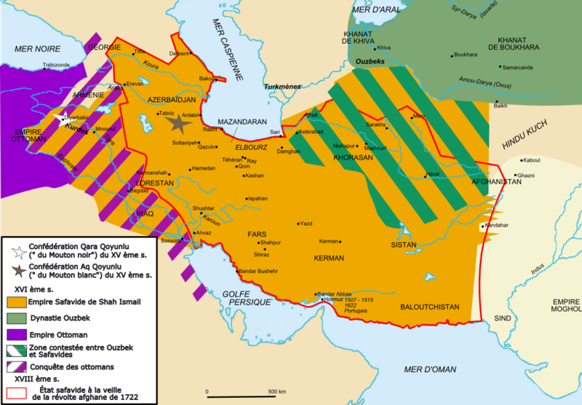
\includegraphics[width=0.9\textwidth]{CourantsIslamContemporain/ImagesCourantsIslamContemporain/empireSafavide.png}

    
\end{figure}


\begin{figure}[h!]
    \centering
        \sidecaption{Apogée et perte de l'empire Moghol : Au XVIII, il est réduit au Rajastan.
}
 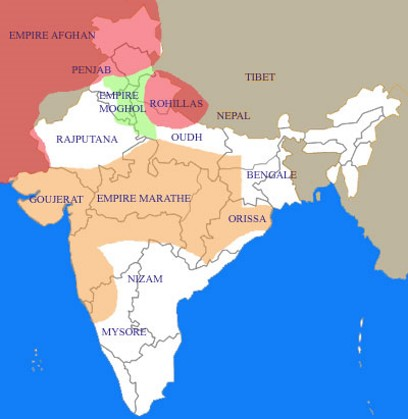
\includegraphics[width=0.44\textwidth]{CourantsIslamContemporain/ImagesCourantsIslamContemporain/Inde18.jpg}
  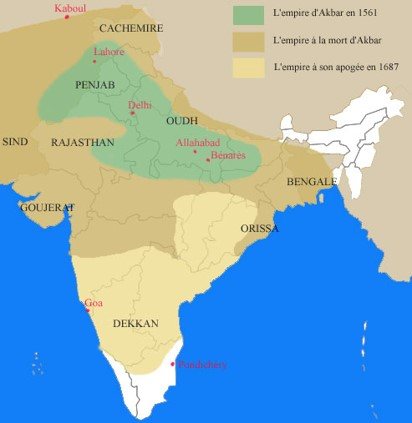
\includegraphics[width=0.44\textwidth]{CourantsIslamContemporain/ImagesCourantsIslamContemporain/empireMoghol.jpg}
\end{figure}

\begin{figure}[h!]
    \centering
        \sidecaption{Déclin Empire Ottoman
}
 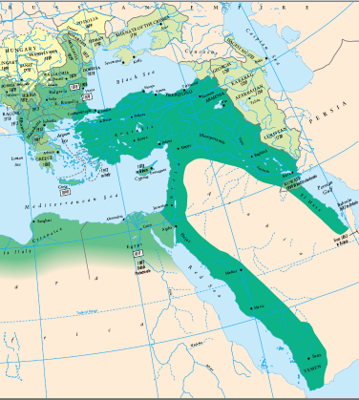
\includegraphics[width=0.5\textwidth]{CourantsIslamContemporain/ImagesCourantsIslamContemporain/declinEmpireOttoman.png}
\end{figure}
 
 \paragraph{Raisons économiques} Les portugais contournent l'Afrique et contournent les empires musulmans.  
 \paragraph{crises politiques} au sein de ces empires, trop grands. 
 \paragraph{Des voisins puissants} Ces Etats vont perdre des territoires face à des puissances qui ne sont pas musulmanes. L'empire Safavide est attaqué par les Ousbeks. L'Empire Moghol en XVIII siècle s'effondre devant l'empire Marathe (Hindou). L'empire Ottoman resiste mais décline depuis 1686 (siège de Vienne). 
 \begin{itemize}
     \item  {Affaiblissement des sultanats Indonésiens} face aux Hollandais. Java est annexé en 1800. 
  \item {En Chine} les musulmans Chinois (Hui) subissent des pressions des Manchous.
   \item  {Afrique} Les bambaras conquièrent Djenné, Tombouctou et Gao. Les portugais en Océanie. 
  \item {En Asie Centrale}, avancée des Russes (XIVII : Kazakstan et reste de l'Asie Centrale au XIX).
 \end{itemize}

 \paragraph{A la fin du XVI} 1591 : deuxième millénaire de l'Islam; sentiment millénariste. \mn{Calendrier lunaire, donc décalage}
 
 
 
\subsection{Problèmes doctrinaux et religieux}

\paragraph{Un raidissement des écoles juridiques au XVII}
Elles s'accusent les unes les autres de ne pas être juste, sentiment de division du monde sunnite.

\paragraph{Décadence du monde Soufi} On a tendance à considérer les soufis comme à la marge du monde musulman. Pourtant, elles ont joué un rôle social déterminant voire politique. Or, à l'époque, elles sont en crise.
\begin{itemize}
    \item {En faisant des Etats dans l'Etat} 
\item {Laxisme spirituel} Un soufi n'est plus tenu de suivre les prescriptions de l'Islam.
\item {Un rôle de plus en plus important du Sheykh}, le maitre spirituel de la Confrérie, qui transmet la \emph{Baraka}.
\item {Des pratiques spéctaculaire} Le fakirisme. le \emph{Dhikr}, rappel du nom de Dieu et l'on atteint l'Etat de transe, et vont marcher sur des braises. 

\end{itemize}



%------------------------------------------------
\section{L'aspiration au
  renouveau}
\subsection{Millénarisme}


 \begin{Def}[rapport au temps Involutif]
 L'Islam se tourne vers le passé, en Islam, les prophètes viennent toujours rappelés ce qui a été donné à l'origine. et le problème est que les hommes déforment le message transmis. Donc Dieu envoie de nouveaux prophètes pour restaurer le message originel. \textit{le temps corrompt.}
 
 \end{Def}
 vs Evolutif. 
 
 Ce qui fait que Mohammad est le dernier des prophètes, c'est que le message est transmis intact, pour la première fois, donc plus besoin de nouveaux prophètes. Autant, la \textit{pratique} peut se corrompre. 
 Un hadith dit : 
 \begin{quote}
     Slt un dixième de la pratique suffira pour sauver le monde.
 \end{quote}
 
 \begin{Def}[Moujaddid]
 de la racine JDD, nouveau, celui qui renouvelle l'Islam pour le mettre tel qu'il était à l'origine. 
 \end{Def}

 
 \begin{Def}[tajdid]
 Tajdid, le renouveau, qui doit venir régulièrement. Chaque siècle Dieu envoie un \textit{Moujaddid} selon un Hadith du Prophète.
 \end{Def}
 
 
 Il peut y en avoir plus mais à chaque siècle, il y a un grand moujaddid, savant, qui ne fait pas forcément au sein de la communauté. 
  \begin{Ex}
 Ghazali est considéré comme un Moujaddid
 \end{Ex}
 \sn{On retrouve cette tension dans toute religion entre respect de la forme et de fidélité au message d'origine}
 
 \subsection{Quelques grandes figures de la \textit{pre-Reforme}}
 

\paragraph{Ahamad Sirhindi} (Inde, 1564-1624) , essaye de rénover l'Islam et réforme une confrérie, la \emph{Naqshbandiyya} réformée (mujaddidi). 
\paragraph{Muhaddidi} Restaurer le monde musulman et restaurer l'Islam dans sa pureté originelle. Il va opposer 
\begin{itemize}
    \item le \emph{taqlid}, l'imitation (péjorative, servile, non réfléchie) et
    \item l'\emph{ijtihad}, l'effort d'interprétation du Coran et de la Sunna. Retourner aux sources scripturaires pour restrouver le sens authentique de l'Islam
    \item pour éliminer la \emph{bid'a}, très péjoratif, l'innovation
\end{itemize}  

On peut distinguer deux courants : un courant plus libéral et l'un plus fondamentaliste :
\begin{itemize}
    \item le rapport à la Tradition : fondamentaliste ne vont considérer que le Coran et la Sunna, en critiquant les élaborations savantes de l'Islam. 
    \item ce sur quoi va porter l'\emph{ijtihad}, soit limité sur les versets peu clairs du Coran, soit plus large pour le savant et les différentes sciences qui vont être convoquées pour l'ijtihad.
\end{itemize}


\paragraph{Muhammad 'Abd Al-Wahhab } 'Arabie, 1703-1792). Voir p. \pageref{Theol:AlWahhab}

\paragraph{Shah Wali Allah} (Inde, 1703-1762), \label{Theo:waliAllah} a eu les mêmes professeurs que Al-Wahhab ! et l'un des premiers à traduire le Coran dans une langue vernaculaire (en persan). Effort d'acculturation dans le contexte Moghol et Indou. 




 
%------------------------------------------------
\section{Les voies du renouveau} 
\subsection{Les confréries soufies}

La création de néo-confrérie
\begin{itemize}
    \item lutter contre un laxisme moral
    \item lutter contre le pouvoir du Sheykh.
    \item insister sur le côté social, en prenant en charge la société (vs gnosticime ?).
\end{itemize}
\mn{Soufi : \pageref{Def:SoufiNaqchabandiya}, \pageref{Def:Soufiqādirīya} }




\paragraph{Ahmad Al Tijani} (Algérie 1737, 1815). Et fonde la \emph{\textbf{tijaniyya}}, un groupe toujours très présent en Afrique du Nord. Normalement un Sheykh insiste sur la chaine d'initiation qui remonte au prophète. Lui, va être initié directement en rêve par le Prophète.

\paragraph{Abdurrauf al-Singkili} (Aceh, Indonésie, 1615-1693)

\paragraph{Abdelkarim al-Samman} (Soudan, 1718-1776) => sammaniyya

Au sénégal, aussi une confrérie de type réformée. 
\mn{A completer carte Carte moderne. Il y avait 24 confréries soufis en Arabie avant le Wahhabisme}




%---------------------------------------
\subsection{Les centres de pèlerinage : La Mecque et Médine}

La Mecque et Médine jouent un rôle essentiel, du fait du Hajj. Du fait de l'Empire Ottoman, il y a pacification des parcours du pélerinage, par ailleurs incités par l'Empire.
Et par ailleurs, des centres de formation s'implémentent à la Mecque.  On en profite pour étudier. Se croisent des savants de différentes origines.
Non seulement les centres d'étude mais aussi les confréries, avec leur Sheykh les plus importants s'installant à Médine ou la Mecque. Ils sont initiés à l'enseignement Moujaddidi et vont réformer la confrérie à laquelle ils appartiennent, selon un modèle qui se répète.




%------------------------------------------------
\section{Un aspect particulier : les jihads aux marges du monde   musulman} 


\begin{figure}[h!]
    \centering
        \sidecaption{Le « renouveau » des marges du monde musulman (XVIIIe-XIXe
siècle)  \emph{L'atlas de l'islam depuis 1500}, F. Robinson, Nathan, 1987  
Des petits Etats vont se créer sur des bases confrériques et dont la mission de faire le jihad.
}
 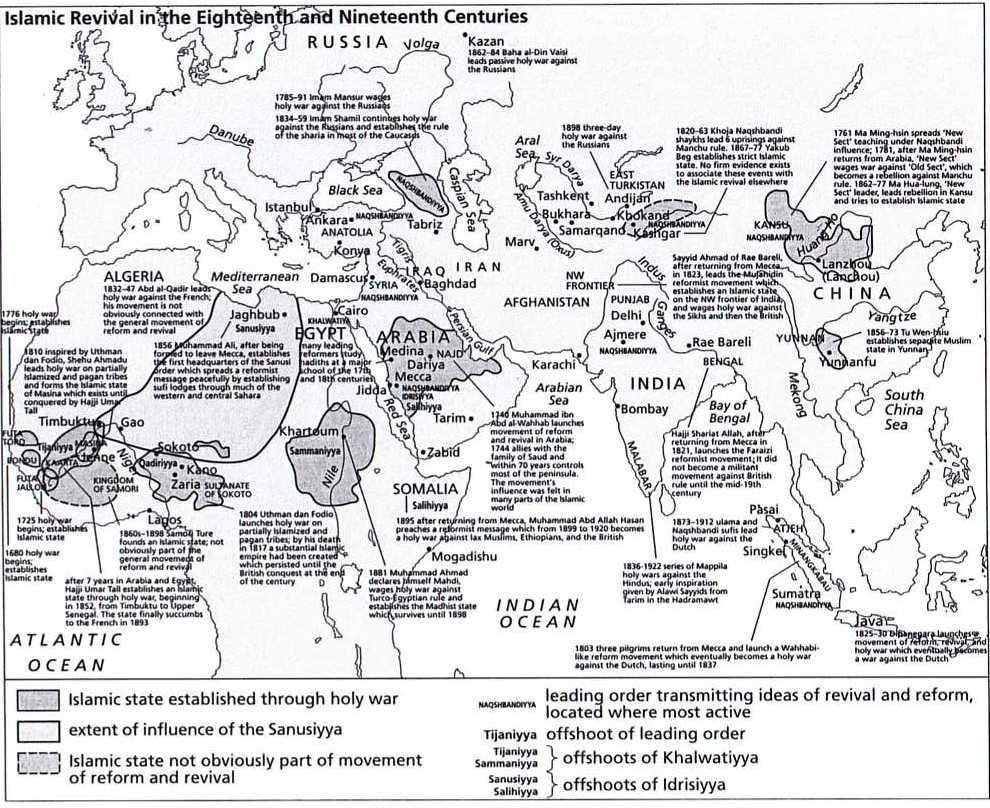
\includegraphics[width=\textwidth]{CourantsIslamContemporain/ImagesCourantsIslamContemporain/image1.jpeg}

    \label{fig:le-renouveau-des-marges-du-monde-musulman-xviiie-xixe-siuxe8cle}
\end{figure}


\subsection{Situation particulière des zones marginales}


Pourquoi on les retrouve aux marges du monde musulman ? Il y a un besoin de purification et l'islamisation par rapport à des populations hétérogènes. Mais aussi, parce que ces zones ne sont pas controlées par les grands empires musulmans qui ne tolèrent pas ces confréries.
Le jihad se porte d'abord sur les musulmans eux-mêmes, pour qu'ils deviennent musulmans puis contre les puissances extérieures ou non musulmanes qui controlent ces zones. 

\paragraph{Une structure Etatique} Le Sheykh est le chef, \emph{Commandeur des Croyants} - on fait référence aux premiers temps musulmans, on prête allégeance, et avec une approche puritaine, très forte pratique. \mn{Des analogiques avec DAESH, qui se réfèrent eux aussi aux temps de l'Islam}

\paragraph{Une accélération de l'Islamisation}


\subsection{Quelques exemples}

\paragraph{Spectre Temporel 1680-1920}{1680, Etat de Bondou} Afrique de l'Ouest jusqu'e l'Etat Mahdiste (Somalie) 1899-1920.

\paragraph{Chine - Ma Ming-hsin} Réveil religieux des communautés chinoises sous la pression des Manchous. Ma Ming-hsin (1719-1781) lorsqu'il est à la Mecque, il fonde une confrérie réformée, la \textit{Nouvelle Secte} et entre en opposition contre les autorités locales, qui appelle en soutien la dynastie Manchoue des Ming. Ming-Hsin est décapité. Il y aura d'autres révoltes plus tard, du Kan-Su et du Chen-Si (1862) et du Yunnan (1856)

\paragraph{Indonésie - Jajji Miskin} Le mouvement Padri à Sumatra (1803-1845). Après le Hajj, en 1803, il prend le contrôle de villages et va imposer sa vision de l'Islam, interdit les pratiques populaires et proclament le Jihad contre les autres villages et les pouvoirs. 1820 : les Hollandais reviennent dans la région et on a une transformation de ce mouvement contre un Jihad contre les Hollandais. Eliminé par les Hollandais.

\paragraph{Nigéria - Califat de Sokoto} Uthman da Fodio (1755-1817) issu d'une famille de savants musulmans, l'enseignement lui vient par la fraderyya\sn{revoir} et crée une communauté qui le reconnait comme \textit{commandeur des Croyants}, s'oppose aux pouvoirs locaux et va être défait par la Grande Bretagne.


\begin{Synthesis}
\begin{itemize}
Ce renouveau : 
    \item Avant la rencontre de l'Occident
    \item lié à des thèmes de crises internes
    \item des thématiques que l'on retrouvera : retourne aux sources scripturaires
    \item C'est assez fascinant de voir la circulation des idées, liée autour du \textit{Hajj}
\end{itemize}


\end{Synthesis}

%------------------------------------------------

 



 



\paragraph{Soufis du Badakhshân : un renouveau confrérique entre
l'Inde et l'Asie centrale}
\mn{Alexandre Papas, \emph{Cahiers d'Asie Centrale}, n° 11-12, 2004, p.
87-102 (extraits -- texte expurgé)}
 
 
\subparagraph{Éléments de biographie d'un soufi
badakhshânais} 
\mn{le Badakhshân est entre l'Afghanistan et le Tajikistan}
\begin{quote}
Mawlânâ Mîr Ghiyâs al-Dîn \label{Theo:MawlanaMirGhiyasAlDin} naît en 1117/1705-06 dans la petite localité
de Hisârak, située au cœur du district de la ville de Jirm. Le
grand-père de Mawlânâ a émigré du village de Dahbîd, non loin de
Samarcande, en direction du Badakhshân. La \emph{silsila}\sn{Génération} de la famille
remonte au Prophète et, sur dix générations, au frère d'un grand saint
Kubrawî et découvre une généalogie \textit{soufie}. C'est donc au sein d'une des
grandes familles \emph{muhâjir}\sn{Emigré, en référence aux premiers musulmans qui ont suivi le Prophète à Médine} de l'aristocratie religieuse du
Badakhshân que naît Ghiyâsî.
\begin{figure}[h!]
    \centering
        \sidecaption{Asie Centrale. On oublie parfois le rôle important de ces états tampon comme lieux d'échange
}
 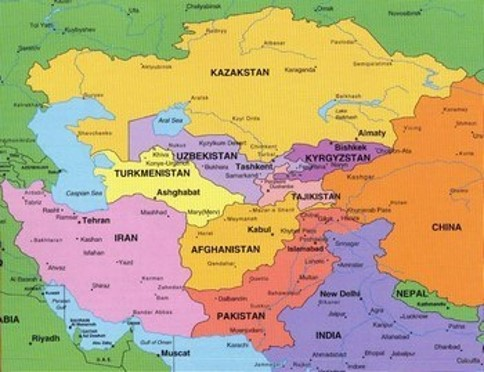
\includegraphics[width=\textwidth]{CourantsIslamContemporain/ImagesCourantsIslamContemporain/AsieCentrale.jpg}
 
\end{figure}

{[}\ldots{]}

C'est précisément pour l'Inde -- destination qui concurrence la
Transoxiane savante, en particulier Boukhara, surtout depuis le XVIe
siècle -- que part le jeune Ghiyâsî âgé de 14 ans en quête d'initiation \sn{soufi}.
Cet exil de l'adolescent fait l'objet de deux contes hagiographiques :
 

\begin{itemize}
\item
 
  Le futur shaykh de Ghiyâsî, Shâh Walî Allâh, qui a quitté Sirhind pour
  entreprendre un pèlerinage au mausolée de Bahâ' al-Dîn Naqshband\sn{le fondateur de la confrérie réformée Naqshandayyi} non
  loin de Boukhara, stationne au Badakhshân, à Jirm, chez le père même
  de Ghiyâsî. Le shaykh demande alors à ce dernier de lui amener ses
  enfants, mais perçoit par claire-vue qu'on lui dissimule le jeune
  Mawlânâ qui, en état de \emph{majzûb}\sn{Ils peuvent faire des choses indécentes} « ravi en Dieu », suscite la honte de
  sa famille. À sa vue le shaykh indien cite un vers de Ni'mat Allâh
  Walî Kirmânî. Et au jeune Ghiyâsî de prononcer miraculeusement le
  second vers du distique. Walî Allâh annonce alors qu'à son retour de
  Boukhara il prendra le jeune homme comme disciple et l'emmènera en
  Inde.
  
\item
 
  Dès l'âge de 9 ans Mawlânâ refuse les conseils de sa famille et se
  distingue des autres enfants. Plusieurs nuits, au cours de rêves, lui
  apparaît un homme illuminé qui lui enjoint de partir pour l'Inde où
  lui est promise la rencontre d'un grand saint soufi. Malgré le refus
  de ses parents qui souhaitent marier leur fils, Ghiyâsî parvient à
  quitter le Badakhshân quelques années plus tard. Parvenu à Lahore et
  après un nouveau rêve révélateur, il attend de nombreux jours au
  couvent de Khwâja Khwândamîr, un khalîfa de la Naqshbandiyya, jusqu'au
  jour où il rencontre Shâh Walî Allâh.
 
\end{itemize}

 
Restent les faits : après une formation classique en \emph{madrasa} à
Delhi où le novice rencontre ses premiers maîtres, il devient à Lahore
durant douze années le disciple d'un fameux maître Naqshbandî Mujaddidî.
Il interrompt une unique fois son initiation lorsque le shaykh lui
confie la mission de se rendre au Cachemire afin d'aller chercher un
homme qu'on prétend thaumaturge et que Walî Allâh souhaite convertir à
l'islam et initier à sa \emph{tarîqat}\sn{confrérie}. Au terme de ses douze années de
noviciat, le shaykh lui enjoint de retourner à sa terre natale pour
propager la confrérie. De retour au Badakhshân, Ghiyâsî âgé de trente
ans environ et qui a obtenu le rang de \emph{mawlawiyyat}\sn{maître}, fait office
d'enseignant à la \emph{madrasa} Jâmi'-i Islâmî du district de Jirm. Il
est ensuite convié à Fayz Âbâd à la cour de Sultân Shâh, laquelle abrite
des savants et des poètes venus d'Inde et d'Iran, dont certains
acquièrent grande réputation. C'est là que Ghiyâsî compose son œuvre
poétique et mystique. C'est également là, de son \emph{khânaqâh}\sn{couvent soufi, Ḵānqāh ou ḵānāqāh, fut d'abord un lieu destiné à abriter les spécialistes et savants religieux musulmans (‘ulamâ’), une sorte d'équivalent des couvents chrétiens. Ces établissements ont été ensuite réservés aux soufis.}, qu'il
dirige son enseignement, suivis par de nombreux disciples venus de
toutes les régions alentours. Le soufi badakhshânais devient aussi le
directeur spirituel de Sultân Shâh. Et lorsque ce dernier est capturé à
Qunduz par les ouzbeks du Qataghân en 1179/1765, le vieux maître
conseille durant trois ans le fils et suppléant du shah emprisonné, Mîr
Muhammad Shâh. D'un tel succès et d'une telle influence, Ghiyâsî
apparaît comme l'un des principaux promoteurs de la Mujaddidiyya dans le
Nord de l'Afghanistan.

{[}\ldots{]}
\end{quote}

\begin{Prop}
On retrouve des noms : Walî Allâh (cf p. \pageref{Theo:waliAllah}; l'importance du réseau confrérique; et rôle social (il devient le conseil du sultan).
\end{Prop}

\subparagraph{Savants et soufis au croisement du
Badakhshân}
Le Pamir est un sanctuaire pour les savants hétérodoxes ou bannis (cf Unwân banni d'Egypte du fait de sa lutte sociale).

\begin{quote}
Malgré les obstacles géographiques et en dépit des troubles politiques
qui affectent la fin du XVIII\textsuperscript{e} siècle, le Badakhshân
reçoit la visite de savants religieux qui, pour certains, décident de
s'y installer et interrompent définitivement leur voyage vers l'Inde ou
vers la Transoxiane. Il faut rappeler ici que le Pamir a, de façon
continue dans l'histoire, servi de sanctuaire à des individus frappés
d'ostracisme ou fuyant la répression dans leur région natale. Mais au cours du
XVIII\textsuperscript{e} siècle le sanctuaire se mue en lieu de
renaissance où fleurissent \emph{madrasa}\sn{lieu d'enseignement religieux} et couvent soufis. Le
\emph{Armaghân-i Badakhshân} mentionne le cas de deux étudiants de
Peshawar, Mîr Ahmad Mujaddidî dit `Izhâr' (m. 1259/1843) et son frère
Muhammad Anwar qui, à une date indéterminée durant le règne de Mîr
Muhammad Shâh, se rendent d'abord à Boukhara afin d'obtenir les
compétences du rang de \emph{`âlim}\sn{savant} et qui, lors de leur retour,
s'installent et officient au Badakhshân, pour le premier à Jirm, pour le
second à Bahârak.

Un autre cas de figure est celui, analogue à Ghiyâsî, de ces
badakhshânais qui partent se former aux sciences religieuses, et
éventuellement au soufisme, dans les grands centres de savoir du monde
musulman, proches ou lointains. De ce point de vue, le cas le plus
intéressant -- et malheureusement le plus douloureux faute
d'informations suffisantes et dans l'absence de vestiges de son œuvre --
est celui de Sayyid Abâ al-Hasan « `Unwân ». Né à Jirm en 1123/1711, il
quitte le Badakhshân pour Boukhara afin d'acquérir une formation
théologique. De là `Unwân se rend au pèlerinage de La Mecque et à
Médine, puis il s'installe durant 18 ans en Egypte, probablement au
Caire, où il poursuit son acquisition des sciences islamiques classiques
et commence à enseigner. Mais `Unwân ne se contente pas de dispenser un
enseignement religieux, il prend parti pour les classes populaires
égyptiennes et contre leur oppression par les propriétaires terriens.
C'est du moins la réputation qu'il gagne selon le \emph{Armaghân-i
Badakhshân}, et qui lui vaut d'être banni d'Egypte. `Unwân part alors
pour Istanbul, rejoint Boukhara et reprend son enseignement. `Unwân, qui
prône l'unité de la Communauté des Croyants (\emph{umma}), décide
d'aller prêcher la concorde (\emph{âshtî}) dans le Caucase, peut-être au
moment de l'activisme Naqshbandî de Shaykh Mansûr dans les années 1780.
Mais il renonce à son projet et entre dans une retraite spirituelle
jusqu'à sa mort en 1206/1791, sans être retourné au Badakhshân.
{[}\ldots{]}

\end{quote}

\begin{Prop}
 Dans le deuxième paragraphe, `Unwân se forme à la Mecque et Médine (rôle du pélerinage), rôle social en Egypte et pas seulement religieux. L'importance aussi de l'Unité, l'\textit{Umma}. 
\end{Prop}
 
\subsection{Liste des neo confréries}

\paragraph{Naqshbandiyya}: La Mecque, Damas, Yémen, Inde, Asie Centrale \label{Def:Naqshbandiyya}
                     => Caucase, Chine Occidentale + Orientale, Sumatra.

\paragraph{Qadiriyya}: Proche Orient, Irak, Inde, Asie centrale 
                    => Indonésie (Java, Aceh), Caucase, Afrique

\paragraph{Khalwatiyya}: Egypte => nombreuses branches en Afrique :

\begin{itemize}
    \item \textit{Tijaniya}: Algérie => Afrique de l’Ouest
    \item \textit{Sammaniyya}: Soudan
    \item \textit{Idrisiyya}: Maroc => Sanusiyya (Lybie), Sahiliyya (Somalie),
    \item \textit{Murghaniyya} (Erythrée)
\end{itemize}- 
 
%-----------------------------------------------
\subsection{bibliographie}

\begin{quote}


AZRA, Azyumardi \emph{The Origins of Islamic Reformism in Southeast
Asia}, Asian Studies Association of Australia/KITLV Press, Leiden, 2004.

PAPAS, Alexandre \emph{Soufisme et politique entre Chine, Tibet et
Turkestan}, J. Maisonneuve, Paris, 2005.

*ROBINSON, Francis \emph{Atlas de l'Islam depuis 1500}, Nathan, Paris,
1987 (dispo à la FELS)

*VOLL, John R. « Foundation for renewal and reform », in John L.
Esposito ed., \emph{Oxford History of Islam}, Oxford University Press,
1999, pp. 509-547.
\end{quote}
\chapter{Un fruit du « pré-réformisme » : le wahhabisme}
\mn{ \emph{(31/01/2022)}}

%---------------------------------------------------------
\section{Le wahhabisme}
\paragraph{Pourquoi en parler} C'est un courant qui a presque trois siècles, avec une évolution dans le monde du musulman qui a évolué. Il faut penser l'Islam contemporain dans son contexte.

 
  \subsection{Muhammad Ibn al Wahhab
  (1702-1792)} 
  \label{Theol:AlWahhab}
  
\paragraph{Origine} Son père est \emph{qadi}\sn{juge} et enseignant. Dans le Hadz. Fait un pélerinage à la Mecque. Renouveau

\paragraph{Formation et premières prédications} Proclame le \emph{Tawhid} l'unicité et lutte contre toutes les pratiques "déviantes". Il se heurte aux autorités locales et retourne donc à la Mecque. Il se forme là avec des maîtres d'Arabie et Indien. Puis se rend à Basra, à un autre maître. C'est là qu'il rencontre les si'ites. Il se heurte de nouveau aux autorités locales. Il rentre en Arabie mais \textit{son père y est hostile}. Ce n'est pas un grand savant mais un lettré. 
 
\paragraph{L'alliance avec Ibn Se`ud} Alliance matrimoniale avec un chef de tribu de la Mecque. Il se rend indésirable et il est obligé de partir et il arrive dans le village de Dariya et il y rencontre un autre chef de village, Mohammed Ibn Se'ud, alliance elle aussi politicolo-religieuse et matrimoniale en 1744. Ibn Se'ud accepte la doctrine et al Wahhab légitime l'acquisition de terre par Ibn Se'ud. 

Wahhab enseigne beaucoup  : il écrit beaucoup à des savants (\emph{Oulema}) à l'intérieur et l'extérieur du royaume de Ibn Se'ud. \textit{selon un modèle prophétique}, Mohammad ayant écrit au Basileos,... 

\paragraph{Un développement politique} Conquiert toute l'Arabie Saoudite. En 1818, c'est la fin du premier état wahhabite car l'empire ottoman intervient et execute le fils de Ibn Se'ud.
    
 Il s'appuie sur deux auteurs : 
\begin{itemize}
    \item Ibn Taymiyya (1263-1328), \label{Theol:Taymiyya2} \sn{cf p. \pageref{ibn-taymiyya}}, un vrai penseur
    \item Ibn Qayyim (1292-1350) un de ces disciples
\end{itemize}
 
Ibn Wahhab insiste sur le retour à la source mais en fait il lit le Coran à travers ces deux auteurs.

\paragraph{Une doctrine condamnée} Son père et son frère s'opposent à lui. Une fatwa contre lui du fait de sa critique sur les différentes écoles juridiques et le fait qu'il exclut de la communauté musulmanes ceux qui ne pensent pas comme lui. 

  \subsection{La doctrine wahhabite} 



  \paragraph{Nécessité du retour aux sources} Accentuation des sources, bien sûr le Coran. 
  \begin{itemize}
      \item  \item  Wahhab s'éloigne d'une lecture du Coran ligne à ligne mais propose une analyse \textit{thématique}.
  \item Il rejette aussi le besoin d'une \textit{médiation} humaine pour comprendre le Coran. Il s'oppose aux \emph{Ashraf}, les descendants du prophète \sn{Les Ashrafs ont un statut particulier dans l'Islam} ainsi qu'aux \emph{Imams} dans le si'isme, ainsi que les \emph{sheykhs} soufis.
  \begin{Prop}
  Il n'y a pas besoin de sciences particulières pour accéder au sens du Coran, d'après Wahhab. 
  \end{Prop}
  \item il suis les \emph{Hadiths}, la seule exégèse possible, la \textit{sunna} et rejette les grands commentaires classiques du Coran.  Cela va jusqu'à critiquer la tradition des 4 premiers Califes \textit{bien guidés}. Abu Bakr avait détourné la \textit{zakat} pour ses propres dépenses.
  \item Il reprend la distinction d'Ijtihad, qu'il limite aux versets aux versets obscures, contre le taqlid. Il s'oppose à deux principes de l'Ijtihad : qiyas (recours par analogie : alcool et drogue), \textit{ijama} (consensus des savants : on considère que cela fait autorité \sn{Infaillabilité de la communauté dans les Hadiths}), et le \textit{ra'y}, l'opinion personnelle du juriste. 
  
  \end{itemize}
 
 \begin{Prop}
 Il conteste les principes sous-jacents aux savants qui l'ont précédés. Il y a une tension entre son ambition de revenir au Coran mais en parallèle en se mettant en filiation avec Ibn Taymiyya
 \end{Prop}
 
 
  \paragraph{Une notion centrale : le \emph{tawhid} (unicité divine)}
  
  \mn{{Extraits du \emph{Kitab at-tawid} (Livre de
l'unicité divine) de Muhammad Ibn Wahhab} . {Chapitre 1} : \emph{Tawhid}
Traduction et édition établies en Arabie Saoudite. Allah est traduit par Allah et non Dieu, alors qu'en Arabe, Dieu est traduit par Allah y compris pour les chrétiens arabes. }

\begin{quote}
\emph{Allah-ta`ala} a dit : « Je n'ai créé les djinns et les hommes que
pour qu'ils M'adorent (1 :56)\ldots Et très certainement nous avons
suscité dans chaque communauté un message pour leur dire d'adorer Dieu
et d'écarter le Rebelle (16 :36)\ldots Et voilà que ton Seigneur a
décrété que tu dois n'adorer que Lui et faire preuve de bonté envers tes
parents (17 :23)\ldots Adorez Dieu et ne lui donnez quelque associé que
ce soit (4 :36)\ldots Venez, je vais vous réciter ce que votre Seigneur
vous a interdit ; - ceci : Ne lui associez quoi que ce soit\ldots(6
:151-153) ». Ibn Mas`ud a dit : « Quiconque se propose de vérifier le
testament du Prophète Muhammad (SWA) -- un testament sur lequel le
Prophète a apposé son sceau, qu'il lise ces mots d'Allah : « Venez, je
vais vous réciter ce que votre Seigneur vous a interdit ; - ceci : Ne
lui associez quoi que ce soit\ldots Voilà ce qu'il enjoint » (6 :
151-153)


Mu`adh Ibn Jabal raconta : « Je montai derrière le Prophète (SAW) quand
il me dit : « Ô Mu`adh ! Sais-tu ce que les créatures d'Allah Lui
doivent et ce qui leur est dû ? » Je répondis : « Allah et son Prophète
savent mieux ». Il continua : « Ce que les créatures d'Allah Lui
doivent, c'est de ne jamais associer qui que ce soit avec Lui. Ce qui
leur est dû, c'est qu'il ne punira aucune personne qui ne Lui associe
pas un autre ». Je dis :

« Ô Prophète d'Allah, est-ce que je peux annoncer la bonne nouvelle aux
gens ? » Il répliqua : «Non ! Ne leur dis rien de peur qu'ils comptent
sur la promesse et manquent à leurs devoirs envers Lui». Ce hadith est
mentionné dans deux \emph{Sahihs}.


D'autres points :


\begin{enumerate}

\item
  \begin{quote}
  La sagesse dans la création du djinn et de l'humanité.
  \end{quote}
\item
  \begin{quote}
  Le service à Allah consiste en le \emph{tawhid}. Car, à l'opposé du
  \emph{tawhid} se trouve l'aliénation d'Allah. (\ldots)
  \end{quote}
\item
  \begin{quote}
  La sagesse d'envoyer des prophètes. (\ldots)
  \end{quote}
\end{enumerate}
  \end{quote}
  
On trouve une accumulation de versets coraniques sur le thème, puis des hadiths du prophète. Le grand péché par excellence, c'est le \emph{shirk}, l'associationisme des Dieux à Dieu. Or Wahhab va plus loin. 

\begin{quote}


\emph{Allah-ta`ala} dit : « Ceux qui ont cru et n'ont point revêtu de
prévarication leur foi\ldots{} » (6 : 82).

(\ldots) Abu Sa`id al Khudriyy rapporta que le Prophète d'Allah (SWA) a
dit : « Quand Musa {[}Moïse{]} demanda à Allah de lui enseigner une
prière qu'il puisse réciter à chaque fois qu'il pensait à Lui ou qu'il
L'évoquait, Allah répondit : « Dis, ô Musa, qu'il n'y a d'autre Dieu
qu'Allah. Musa dit : « Ô Seigneur, tous tes serviteurs prononcent ces
mots ». Allah dit : « Ô Musa, si les sept cieux et tout ce qu'ils
renferment, et les sept terres aussi, si tout cela était pesé contre
cette phrase : « Il n'y a d'autre Dieu qu'Allah », cette dernière
pèserait plus lourd ». Ibn Hibban rapporta cela également et al-Hakim
compléta sa version. Al-Tirmidhi enregistra, avec peu de rédaction, le
récit de Anas à l'effet qu'il entendit le Prophète d'Allah (SWA) dire :
« Allah dit : « Ô Homme ! Si tu venais à Moi avec tous les sacs du monde
remplis de tes péchés, mais avec le témoignage que tu n'associes rien à
Moi, Je viendrais à toi avec tous mes sacs remplis de miséricorde et de
pardon ! ».

    
\end{quote}

\begin{Synthesis}
Si on respecte le \emph{Tawhid}, cela suffit à pardonner les péchés, mais important de respecter les principes de l'Islam (c'est pour cela que c'est caché)
\end{Synthesis}

\paragraph{Distinction au sein du Tawhid } 
\begin{Def}[Le grand Shirk ]
Il distingue le \emph{tawhid rububiyya} (l'unicité de souverainté du monde) avec le \emph{tawhid uluhiyya} (de divinité) : ne reconnaitre aucun intermédiaire entre Dieu et les hommes. Il ne peut y avoir de dévotion que pour Dieu seul : les saints, les soufis, les Imams.
\end{Def} 
Al Wahhab introduit une critique fondamentale contre le soufisme. 

\paragraph{Le petit Shirk} 
\mn{{Chapitre 4} : La crainte du \emph{shirk}}
\begin{quote}
Allah -- qu'Il soit loué et glorifié -- dit : « Non, Dieu ne pardonne
pas qu'on Lui donne quelque associé. En deçà, Il pardonne à qui il veut
» (4 : 48, 116)

(\ldots) Dans le hadith, nous lisons : « Ce que je crains le plus pour
vous, c'est le moindre \emph{shirk}. Quand on lui demanda ce que
c'était, le Prophète répondit : « l'hypocrisie ». Dans le Sahih
d'al-Bukhari, nous lisons que Ibn Mas`ud reporta : « Le Prophète d'Allah
(SWA) a dit : « Celui qui rencontre Allah le jour du Jugement sans Lui
avoir associé qui que ce soit ira au Paradis, et celui qui le rencontre
ayant fait le contraire sera consigné en Enfer ».
\end{quote}
\begin{Def}[le Petit Shirk]
Toute attitude de l'homme qui ne sert pas Dieu. il relève aussi de l'attitude morale.
\end{Def}

\begin{Ex}[L'appel à témoigner qu'il n'y a d'autre
Dieu qu'Allah]

\mn{{Chapitre 5} : }
\begin{quote}
\emph{Allah-ta`ala} a dit : « Dis (ô Muhammad) : `\,`Voici mon sentier,
j'appelle à Dieu'\,' » (12 :108)

Ibn `Abbas (RA) rapporta : « Quand le Prophète d'Allah (SAW) envoya
Mu'adh à al-Yaman, il lui recommanda : `\,`Quand tu rencontres des gens
du Livre, que ta première action soit de leur demander de témoigner
qu'il n'y a d'autre Dieu qu'Allah'\,' ». Selon un autre récit, «
\ldots{} de leur demander de réaliser l'unicité d'Allah. S'ils
t'obéissent, informe-les qu'Allah leur a imposé la \emph{salat} cinq
fois par jour. S'ils t'obéissent en cela, alors informe-les qu'Allah
leur a imposé le devoir de charité qui doit être perçue des riches pour
être distribué aux pauvres. S'ils t'obéissent en cela, ne touche pas à
leurs autres biens et occupe-toi de la plainte de l'opprimé, car il n'y a aucun obstacle dans son accès à Allah ».
(Rapporté dans les \emph{Sahihs} d'al-Bukhari et de Muslim). (\ldots)
\end{quote}
\end{Ex}



\paragraph{Les Intercessions} L'intercession est limitée à Mohammed, et uniquement aux musulmans suivants Wahhab. On ne peut pas prier le Prophète. Peut être intervient-t-il au jugement dernier.


\mn{{Chapitre 17} : L'intercession}
\begin{quote}
Allah -- qu'il soit loué et glorifié -- a dit : « Et par ceci (le
Qur'an), avertis ceux qui, n'ayant pour eux hors de Dieu, ni ami ni
intercesseur, craignent d'être rassemblés vers le Seigneur\ldots{} » (6
: 51). Dis : « A Dieu l'intercession tout entière\ldots{} » (39 : 44).
Qui peut intercéder auprès de Lui que par sa permission ?... (2 : 255).
Et combien d'anges dans les cieux ? Leur intercession ne met au large en
rien, sauf après que Dieu l'a permis, en faveur de qui il veut et qu'il
agrée » (53 : 26). (\ldots)

(\ldots) En tant que catégorie générale du Jour du Jugement en laquelle
les mécréants croient, l'intercession est rejetée par le Qur'an. Le
Prophète (SAW) nous informa qu'en ce jour « il sera amené devant Allah.
Il se prosternera lui-même et louera Allah, plutôt que de demander à
intercéder. Alors on lui dira : « Lève-toi ! Parle maintenant et tu
seras entendu ! Demande et il te sera donné ! Intercède et il te sera
accordé ! » (\ldots) L'intercession est donc là pour les croyants
sincères et candides. Elle n'est accordée que par la permission d'Allah
et n'appartient pas aux associationistes. (\ldots)
\end{quote}


\paragraph{Tombe du juste}
Condamnation de celui qui invoque Dieu
auprès de la tombe du juste et, a fortiori, de celui qui invoque ce
dernier.
\begin{Ex}[Un exemple de Grand Shirk]
\mn{{Chapitre 20} : Condamnation de celui qui invoque Dieu
auprès de la tombe du juste et, a fortiori, de celui qui invoque ce
dernier.}
\begin{quote}
Dans le \emph{Sahih}, A'ishah (RAA) rapporta : « Umm Salmah raconta au
Prophète d'Allah (SAW) qu'elle avait vue une église remplie d'images et
de statues en Abyssinie. Le Prophète dit : « Ceux-là sont les pires de
tous les hommes : lorsqu'un membre juste et vertueux de leur groupe
meurt, ils bâtissent une église sur sa tombe et y installent toutes
sortes d'images pour lui. Ils sont coupables de deux méfaits : celui
d'invoquer quelqu'un auprès d'une tombe et celui d'installer des images
». (\ldots)

Ainsi le Prophète interdit cette pratique et condamna celui qui la
suivait. Faire le \emph{salat} sur une tombe est également interdit,
même si aucune mosquée n'a été construite sur l'emplacement. Telle est
la signification de la déclaration suivante : « On craignait qu'elle ne
soit prise pour une mosquée ». Les Compagnons n'étaient pas supposés
construire une mosquée autour de la tombe du Prophète. Tout endroit
destiné au \emph{salat} ou tout endroit où le \emph{salat} est accompli,
est une mosquée. Tel l'a déclaré le Prophète (SAW) : « Toute la terre
est pour moi une mosquée, un endroit pur (pour accomplir le
\emph{salat}) ».
\end{quote}

\end{Ex}


  \paragraph{La question du \emph{jihad}} La question de la violence chez Wahhab. Il faut repartir de la position kharijite. Un calife doit respecter la religion de façon exemplaire. s'il ne le fait pas, il est \emph{Takfir}, mécréant. Or la vision sunnite a jugé que c'est Dieu uniquement qui jugera si un musulman est un non-musulman. Ibn Taymmayyia s'élève contre les souverains Mongols : : les souverains mongols sont certes musulmans puisqu'ils ont adopté la foi musulmane mais en surface.  Wahhab va reprendre ce concept et ceux qui n'adhèrent par au \emph{shirk} sont apostats. Un germe de violence.
  
  \begin{Synthesis}
  On voit donc l'extension du concept de Ibn Taymmayyia sur le Takfir à tout le shirk, et donc en pratique en non respect du wahhabisme.
  \end{Synthesis}
 
 Mais il n'y a pas de volonté de jihad dans le wahhabisme. On peut même faire des traités avec des non-musulmans.
 
  \section{Le devenir du wahhabisme} 
 
  
 

% ------------------------------ 
\subsection{Les trois Etats Saoudiens} 

 
  {\paragraph{1744 -1818}: une première expansion}
 
 
\emph{1744} alliance Ibn Se`ud /Ibn al-Wahhab
 
\emph{1786} conquête du Najd (`Abd-al-`Aziz)
 
\emph{1792} mort d'Ibn al-Wahhab
 
\emph{1806} conquête de La Mecque
 
\emph{1818} défaite devant les Ottomans
 

 
  {\paragraph{1821-1883}: petit Etat centré sur Riyad (Najd)}
 
  {\paragraph{1901- 2011} : le Royaume d'Arabie Saoudite} Un descendant de Wahhab qui repasse alliance avec la famille de Se'ud et conquiert l'Arabie. 
 
 
\emph{1924} conquête de La Mecque. Abdelaziz Ibn Se`ud prend le titre de
roi et \textit{protecteur des lieux saints}. On détruit les confrérie, on contrôle le pélerinage, on supprime les autres écoles de droit.

\mn{REVOIR}

\emph{1939} début de la production pétrolière \emph{1962} création de la
Ligue islamique \emph{1990} début de la guerre du Golfe.
 

 
\subsection{L'Arabie Saoudite et l'économie
pétrolière} 
 
\paragraph{ {Début de la
production}} 

\begin{quote}
1935: premier forage

1939: premier baril de pétrole

⇒ Cartel américain: l'ARAMCO
\end{quote}

 
\paragraph{{Nationalisation de la
production}}


1973: l'Etat s'approprie 25 \% des droits de l'ARAMCO (1974 : 60\%, 1980 : 100\%)


⇒ Saoudi ARAMCO: 95 \% de la production du pays.

 
\paragraph{Evolution du cours du
pétrole} 

\begin{quote}
1973: premier choc pétrolier (guerre de Kippour) =\textgreater{} de 4 à
15 \$/B

1981-1983: deuxième choc pétrolier (Révolution iranienne + guerre
Iran-Irak) =\textgreater{} 36 \$/B 2006-2008: troisième choc pétrolier
(guerre en Irak) =\textgreater142 \$/baril
\end{quote}

\paragraph{{Rente}}: 1973-2002 =\textgreater{} 200 000 milliards
de dollars au total
 
    Une étude de cas : le wahhabisme en Afrique de l'Ouest
    
\subsection{Le wahhabisme et l'Etat saoudien}

Le wahhabisme accepte une certaine ouverture en Arabie en contrepartie de financement extérieur. On est dans des \textit{concessions} des oulemas. 

\paragraph{La ligue islamique 1962} on étudie gratuitement à la Mecque et à Médine pour propager le wahhabisme.

 
\subsection{Une étude de cas : le wahhabisme en Afrique de l’Ouest}

\paragraph{Des étudiants revenant de la Mecque dans les années 40} et surtout depuis dans les années 70, avec la ligue islamique. 

\paragraph{Un conflit avec les structures soufis}, maraboutisme, très puissantes. On ne priait pas dans les mêmes lieux de culte. 1978 : On  est  loin de  l'époque  où,  en  1978,  Yao  Koum  expliquait  au  Ministre  de  l'Intérieur  qu' \sn{Le wahhabisme à Abidjan Marie Miran-Guyon \url{https://halshs.archives-ouvertes.fr/halshs-01062687/document}}
\begin{quote}
    "obliger  un musulman  orthodoxe (wahhabite)  à  prier  derrière  un  musulman  traditionnel,  c'est  le  contraindre  à renoncer  purement  et  simplement  à  sa  religion,  c'est  l'anéantir  moralement".
\end{quote}


 % -------------------------
\subsection{ {Glossaire}} 


\paragraph{Personnes} `Abd al --`Aziz Abu Bakr

al-Majmu`i al-Sindi

Ibn Taymiyya Muhammad Ibn Se`ud

\paragraph{Lieux}

al-Azhar al-Dir'iyah

al-Uyaynah (Najd). Basra

Hijaz Huraymila Jeddah Najd

\paragraph{Notions}

ashraf : \emph{descendants du Prophète}

da`wa \emph{: prédication}

fiqh : \emph{droit musulman}

hadith \emph{: fait ou dire du Prophète}

hijra : \emph{« exode »}

ijma\emph{` : consensus des ulamas}

ijtihad : \emph{effort d'interprétation}

kufr \emph{: incroyance /} 

kafir \emph{: infidèle, mécréant}

qiyas \emph{: raisonnement par analogie}

salat : \emph{prière rituelle} 

shirk : \emph{associationnisme} 

taqlid
\emph{: imitation (servile)} 

tawhid : \emph{unicité divine}

zakat :
\emph{aumône légale}

 %-----------------------------------------------------
\subsection{Extraits du \emph{Kitab at-tawid} (Livre de
l'unicité divine) de Muhammad Ibn Wahhab}
\mn{Traduction et édition établies en Arabie Saoudite}

\paragraph{{Chapitre 2} : Les vertus du \emph{tawhid} et les
nombreux péchés qu'il expie}



\paragraph{{Chapitre 27} : Les motivations mondaines sont des
exemples de \emph{shirk}}
\begin{quote}
\emph{Allah ta'ala} a dit : « Qui aspire à la vie d'ici-bas et à ses
parures, nous leur solderons ce qu'ils y auront fait : ils ne subiront
pas de perte ! Voilà ceux qui, dans la vie dernière, n'ont pour partage
que le Feu : leurs réalisations d'ici-bas ont crevé ! Nulles sont leurs
œuvres ! (11 : 15-16).

Abu Hurayrah (RAA) rapporta ce hadith \emph{sahih} suivant : « Le
prophète d'Allah (SAW) a dit : `\,`Malheur à l'esclave du dinar !
Malheur à l'esclave du dirham ! Malheur à l'esclave du khamilah !
(\ldots)
\end{quote}
\paragraph{{Chapitre 38} : Obéir aux ulamas ou aux gouvernants
qui légitiment ce qui est interdit ou interdisent ce qui est légitime,
c'est les associer à Allah.}
\begin{quote}
Ibn `Abbas a dit : « Je vous dis que `\,`le Prophète d'Allah (SAW) a dit
ceci et vous dites que `Abu Bakr et `Umar ont dit quelque chose d'autre
?'\,' Le ciel va bientôt vous cracher des pierres sur la tête !! »

Ahmad ibn Hanbal a dit : « Très étranges, en effet, sont ceux qui,
sachant le véritable \emph{isnad} (d'un commandement du Prophète), se
tiennent quand même à l'opinion de Sufyan. Allah lui-même a dit : « Que
ceux donc qui s'opposent à son commandement prennent garde qu'une
tentation ne les atteigne, ou que ne les atteigne un châtiment
douloureux ». (24 : 63). Savez-vous ce que peut être une telle tentation
? C'est le \emph{shirk}. Car, désobéir au Prophète dans certains de ses
commandements, c'est pratiquement comme si on reniait son message et on
s'attirait le Feu.

\end{quote}


\section{bibliographie}

 

\begin{itemize}
\item
 
  IBN AL-WAHHAB, Muhammad \emph{L'unicité de Dieu}, al Qalam, Paris,
  2001.
 


 \item
MENORET, Pascal \emph{L'Énigme saoudienne. Les Saoudiens et le monde
1744-2003}, La Découverte, Paris, 2003.
\item
MIRAN, Marie ; RIALLAND, Maëlle « Dossier Wahhabisme », \emph{Islam et
sociétés au Sud du Sahara}, n°12, 1998, Paris.
\item
MOULINE, Nabil \emph{Les Clercs de l'islam. Autorité religieuse et
pouvoir politique en Arabie Saoudite
(XVIII\textsuperscript{e}-XXI\textsuperscript{e} siècles)}, Paris, PUF,
2011.
\item
  \emph{Histoire de l'Arabie
saoudite}, Paris, Flammarion, 2013.
\item
REDISSI Hamadi \emph{Une histoire du wahhabisme. Comment l'islam
sectaire est devenu l'islam}, Paris, Seuil, 2016.
 \end{itemize}
 
 
\mn{
\href{http://journals.openedition.org/assr}{Archives de sciences
sociales des religions} p. 229-253

\url{https://doi.org/10.4000/assr.21954}}

\section{Les oulémas du palais}

Parcours des membres du Comité des grands oulémas

\hypertarget{ruxe9sumuxe9s}{%
\subsection{\texorpdfstring{\emph{Résumés}}{Résumés}}\label{ruxe9sumuxe9s}}


Véritable matrice idéologique de l'État saoudien et instrument de
légitimation politique et religieuse, la doctrine wahhabite et ses
dépositaires, les oulémas, sont les soutiens indéfectibles de la famille
Sa‛ūd depuis la seconde moitié du e siècle. Cette alliance se renforce,
à partir de 1971, avec la création d'un certain nombre d'institutions
politico-religieuses dont la plus importante est le Comité des grands
oulémas. Si les larges prérogatives, dont dispose cette dernière dans
les domaines politique, religieux et social, poussent l'autorité
politique à vouloir en chapeauter l'action et contrôler l'accès,
l'establishment wahhabite n'en fait pas moins. En effet, l'élite
religieuse saoudienne a adopté des mécanismes d'autorégulation bien
définis pour maintenir son homogénéité et son unité pour mieux dominer
l'espace socioreligieux du royaume. Nous tentons dans cet article, à
partir d'une étude de terrain, de lever le voile sur ces mécanismes en
étudiant les origines sociales et régionales et le cursus honorum des
quarante-cinq oulémas qui siègent ou ont siégé au Comité. Cela permet
d'en ressortir avec le portrait idéal-type de l'ouléma wahhabite
contemporain et de voir dans quelle mesure son parcours le qualifie pour
l'encadrement de la population et du soutien au régime.

\hypertarget{texte-intuxe9gral}{%
\subsection{\texorpdfstring{\emph{Texte
intégral}}{Texte intégral}}\label{texte-intuxe9gral}}

\begin{quote}
\mn{ Paris -- Institut d'Études Politiques,
\href{mailto:mohammednabil.mouline@sciences-po.org}{\nolinkurl{mohammednabil.mouline@sciences-po.org}}}

En s'appuyant sur la doctrine hanbalo-wahhabite, pour légitimer leur
pouvoir et leur hégémonie en Arabie et étendre leur influence dans le
monde musulman, les Āl Sa‛ūd se sont étroitement liés aux oulémas,
dépositaires et interprètes de cet «instrument intellectuel par
excellence de domination politique» en Arabie Saoudite (Al Rasheed,
2007: 28). En échange de la garantie d'autonomie de l'espace religieux
et d'un contrôle plus ou moins étroit de l'espace social, les oulémas
mettent au service de la monarchie saoudienne toutes les ressources
symboliques dont ils disposent pour légitimer ses positions et
sanctifier son action. La consolidation définitive du royaume saoudien,
en 1932, n'a fait que renforcer cette alliance et l'institutionnaliser.

Le flux des revenus pétroliers et la politique de solidarité islamique
menée par la
monarchie saoudienne (Kepel, 2003: 89-92; al-Suwayyigh, 1992: 83-93) a
permis à l'establishment hanbalo-wahhabite de se moderniser en se dotant
de structures administratives et éducationnelles dont la plus importante
est le Comité des grands oulémas. 
\begin{Def}[comité des grands oulémas]
Mise en place en 1971, cette instance,
où siègent en théorie les plus éminents oulémas du pays, et même du
monde musulman, s'est très rapidement imposée comme la principale
instance législative du pays, à côté du conseil des ministres, la
principale instance légitimatrice de l'action politique du pouvoir et le
bouclier idéologique du régime. 
\end{Def}

L'importance que revêt cette
organisation étatique fédérative pour le pouvoir politique saoudien
pousse ce dernier à vouloir en contrôler l'accès et le fonctionnement
pour éviter toute «insubordination» des grands oulémas. De même, l'élite
religieuse veille, à travers ses réseaux formels et informels, à
maintenir sa cohésion et son homogénéité, pour perpétuer l'hégémonie de
son discours, en imposant aux prétendants aux charges «cléricales»
officielles des conditions plus ou moins rigoureuses. Toutefois, aucun
document ne mentionne les conditions que doit remplir un ouléma pour
accéder au Comité. Le seul moyen de lever le voile sur ces conditions
d'accès tacites est de suivre le parcours et le processus de
socialisation des cinquante- deux oulémas qui siègent ou qui ont siégé
au Comité. L'étude des origines sociales,
«ethniques» et régionales des oulémas, de leur formation, de leur
\emph{cursus honorum} et de leur mobilité permettront non seulement de
tirer au clair les conditions d'accès à cette élite mais aussi de jeter
de nouvelles lumières sur les principales caractéristiques de ce groupe
stratifié et différencié. Et pour remettre cette élite dans son milieu
sociopolitique, nous ferons appel, à chaque fois que cela sera possible,
aux autres élites
consultatif1 -- dans le cadre d'un travail de comparaison et de mise en
perspective. Cela permettra, d'une part, d'énumérer les principales
conditions, plus ou moins tacites, d'accès à cette élite et son
évolution, d'autre part, de voir dans quelle mesure l'establishment
hanbalo-wahhabite fait preuve d'auto-encadrement, d'autorégulation, de
reproduction et d'adaptation, sous l'œil bienveillant de l'autorité
politique, pour mieux dominer l'espace religieux saoudien et rayonner
dans l'espace islamique.
\end{quote}

\hypertarget{des-self-made-men-aux-huxe9ritiers}{%
\section{Des self-made-men aux
héritiers:}\label{des-self-made-men-aux-huxe9ritiers}}

\begin{quote}
\textbf{origines sociales des oulémas}

La prédication de Muḥammad b. `Abd al-Wahhāb (m. 1792), qui connaît un
succès fulgurant, fait de nombreux disciples. Du vivant d'Ibn `Abd
al-Wahhāb déjà, plusieurs de ses disciples manifestent zèle et grand
dévouement à la \emph{da‛wa}. À la mort du fondateur du
hanbalo-wahhabisme, il y a routinisation de son charisme, au sens de Max
Weber. Si les membres de sa famille héritent d'une grande partie de ce
charisme, ses disciples eux aussi, bénéficient de la routinisation. Il
en résulte la création d'un certain nombre de «dynasties» d'oulémas
monopolisant l'espace religieux (malgré quelques cas isolés de réussite
individuelle) des trois États saoudiens et ce jusque dans les années
cinquante. Ces «dynasties» d'oulémas sont pour les plus importantes, les
Āl al-Shaykh, descendants directs du cheikh Ibn `Abd al-Wahhāb, les Āl
Sulaym, les Āl `Atīq, les Āl Blīhid, etc. (al-Bassām, 1999; Āl
al-Shaykh, 1973). Mais à partir des années cinquante, une certaine
«démocratisation» de la fonction cléricale voit le jour en Arabie
Saoudite. La liste des membres du Comité des grands oulémas, depuis sa
création en 1971, en est la preuve. Il ressort globalement de nos
entretiens et de la lecture des biographies des membres du Comité
décédés à ce jour, 
\begin{Synthesis}
trois grandes catégories d'oulémas: les self-
made-men, les enfants de ceux qu'on a appelés des «cadres religieux
moyens» et les héritiers des grandes «dynasties» d'oulémas.
\end{Synthesis}

Dans la première catégorie, ont été classés les oulémas d'origine
étrangère et les oulémas saoudiens issus de milieux modestes. Faire des
études et accéder aux hautes fonctions religieuses a offert des
opportunités incalculables à ces oulémas et leur a garanti la promotion
sociale. Mais on remarque que ces ascensions sociales restent tout à
fait exceptionnelles. Dans une société qui fonctionne toujours selon le
modèle segmentaire, la mobilité sociale n'est, en théorie, possible que
si l'individu possède un certain capital culturel et social, capital que
les self-made-men ne possèdent naturellement pas. Cela se fait
d'ailleurs ressentir au sein du Comité car, bien que très respectés pour
leurs qualités personnelles et leur savoir, les self-made-men sont,
malgré cela, «dédaignés» par leurs collègues, à cause de leur origine
sociale. D'ailleurs, la nomination de self-made-men au sein du Comité
des grands oulémas n'est intervenue que trois fois depuis la création du
Comité: une première fois en 1971, la deuxième fois, en 1977 pour
remplacer un membre décédé et la troisième fois, lors du premier
remaniement des membres de la Hay'a, en 1987. Cela peut être expliqué
par le fait que l'Arabie Saoudite souffrait d'un manque de cadres entre
les années cinquante et soixante-dix, ce qui a obligé les autorités à
faire appel à des cadres religieux étrangers en attendant la formation
des cadres «nationaux».

La deuxième catégorie, celle des enfants des «cadres religieux
moyens», est constituée d'oulémas dont les parents, au sens large du
terme, ont exercé des fonctions religieuses telles la magistrature,
l'enseignement, l'imamat d'une mosquée ou encore la prédication, sans
toutefois bénéficier d'une grande renommée. Ils peuvent également
descendre de familles d'oulémas «mineures». Nous avons aussi inclus dans
cette catégorie les oulémas dont les parents ont exercé une profession
libérale, tout en ayant une connaissance du Coran et d'une partie de la
production théologique hanbalo-
wahhabite. Les oulémas issus de cette catégorie constituent plus de 67\%
des membres du Comité des grands oulémas.

Le milieu familial joue un rôle déterminant dans la promotion sociale
de ces oulémas.

Les «cadres religieux moyens» initient eux-mêmes leurs enfants au savoir
religieux ou les confient, le cas échéant, à des précepteurs de
confiance. Le réseau parental ou familial leur permet d'étudier avec les
maîtres les plus réputés et les plus influents et de fréquenter les
bibliothèques les mieux fournies. De plus, l'apprenti \emph{`ālim} de la
génération d'avant le boom pétrolier n'est pas obligé de travailler ou
d'entreprendre, parallèlement, d'autres études pour subvenir à ses
besoins. Il est, en effet, important pour les «cadres religieux moyens»
de former le fils «prodige» pour en faire un grand \emph{`ālim}, dans le
but d'assurer la mobilité sociale pour toute la famille. Car il faut
savoir qu'en devenant grand \emph{`ālim} et membre du Comité des grands
oulémas, il devient, par la même occasion, très aisé financièrement et
très influent.

8 Parmi ces oulémas, ceux qui réussissent à avoir un capital symbolique
restent cependant rares. Plus rares encore, sont les oulémas qui
réussissent à transmettre ce capital à leurs héritiers. Si une telle
transmission se fait, nous assistons à la création d'une «dynastie»
d'oulémas. Cela a été le cas de la famille Ibn Ḥumayd. Issu d'une
famille de «cadres religieux moyens», `Abd Allāh b. Ḥumayd (1911-1982) a
gravi un à un tous les échelons de l'establishment religieux. Grâce à sa
proximité avec Muḥammad b. Ibrāhīm (m. 1969), le grand mufti du royaume
et la principale figure du hanbalo- wahhabisme durant la première moitié
du e siècle, Ibn Ḥumayd a réussi à obtenir le poste de juge dans les
principales villes du Najd dès 1939. Son talent et sa loyauté envers la
dynastie ont poussé le roi `Abd al-‛Azīz à le nommer, en 1953, grand
juge de la province du Hijâz et imâm de la grande mosquée de la Mecque
puis responsable de la gestion des deux lieux saints. Ces postes lui ont
conféré une réputation nationale et Ibn Ḥumayd est peu à peu devenu une
personnalité religieuse incontournable dans le royaume. Il atteint le
sommet de sa carrière dans les années soixante-dix en devenant membre du
Comité des grands oulémas et président du Haut conseil de la
magistrature. Si Ibn Ḥumayd n'est pas le seul exemple de réussite dans
le royaume -- Ibn Bāz (m. 1999) et Ibn `Uthaymīn (m. 2001) sont arrivés
au sommet de l'establishment --, son originalité réside dans le fait
qu'il a réussi à transmettre son capital symbolique à son fils Ṣāliḥ.


\paragraph{9 Ṣāliḥ Ibn Ḥumayd}  Né en 1950, celui-ci poursuit, sous l'œil bienveillant de son père,
une double formation traditionnelle et moderne, sanctionnée par un
doctorat en droit musulman. Il commence alors une carrière universitaire
qui le mène rapidement au sommet de l'establishment. En quelques années,
il devient le doyen de la faculté de théologie de l'Université islamique
de la Mecque. Ses nouvelles fonctions et sa connaissance de la langue
anglaise lui permettent de participer à des rencontres internationales
et de donner une image moderne de l'establishment hanbalo-wahhabite.
Parallèlement, il remplace son père à la tête de l'appareil chargé de
gérer les lieux saints. Il reprend par la même occasion le poste très
prestigieux et médiatique d'imâm dans la grande mosquée de la Mecque. En
1993, Ṣāliḥ b. Ḥumayd est nommé membre du Conseil consultatif. En
décembre 2001, il devient membre du Comité des grands oulémas. Quelques
mois plus tard, il prend la tête du Conseil consultatif. En 2009, il
récupère le poste paternel de président du Haut Conseil de la
magistrature. D'ailleurs, Ibn Ḥumayd prépare déjà ses enfants à prendre
la relève: une «dynastie» est née2.
\end{quote}

\hypertarget{les-ux101l-shaykh-les-luxe9vites-du-hanbalo--wahhabisme}{%
\section{Les Āl Shaykh : les Lévites du hanbalo-
wahhabisme}\label{les-ux101l-shaykh-les-luxe9vites-du-hanbalo--wahhabisme}}

\begin{quote}
10 Toutefois le tableau serait incomplet, si l'on omettait de parler de
la plus grande famille religieuse du pays, qui règne sans partage sur
l'establishment religieux depuis le
e siècle. Il s'agit des Āl al-Shaykh, troisième grande famille du
royaume après les Āl
Sa‛ūd et les Sudayrī et descendants directs de Muḥammad b. `Abd
al-Wahhāb. Ses membres détiennent, en effet, les plus hautes fonctions
religieuses. Le capital symbolique de cette famille s'est transmis, sans
interruption, de génération en génération, depuis l'apparition du
hanbalo-wahhâbisme.

11 Après la mort d'Ibn `Abd al-Wahhāb, ses descendants reçoivent une
grande partie de son héritage spirituel et temporel. Ils allaient
apporter à la famille des Āl Sa‛ūd tout l'appui idéologique dont
celle-ci allait avoir besoin pour étendre son influence et son
territoire. Cette «entente cordiale» profite aux deux parties: les Āl
al-Shaykh confèrent la légitimité aux Āl Sa‛ūd qui, en retour, concèdent
aux Āl al-Shaykh le monopole de l'espace religieux. Une alliance
matrimoniale vient renforcer cette alliance politico- religieuse: le roi
`Abd al-‛Azīz, fondateur du troisième État saoudien, épouse la fille du
premier mufti du royaume `Abd Allāh b. ‛Abd al-Laṭīf. De cette union
naîtra Fayçal, roi d'Arabie Saoudite de 1964 à 1975. Cette alliance
connaît toutefois une grave crise dans les années soixante quand le
grand mufti Muḥammad b. Ibrāhīm entrave les projets
«d'institutionnalisation» de son petit neveu (Ibn Ibrāhīm, 1978: no
4033-4039 et no
4539-4046), le roi Fayçal. À la mort d'Ibn Ibrāhīm, le roi bureaucratise
les oulémas: les Āl al-Shaykh sont évincés des principaux postes
religieux3. De 1971 à 1987, seul un membre de la famille Āl al-Shaykh,
Ibrāhīm b. Muḥammad b. Ibrāhīm, destiné initialement à succéder à son
père au poste de grand mufti, exerce une haute fonction étatique. Il est
membre du Comité des grands oulémas et ministre de la justice.
L'humiliation a été grande suite à la nomination, à la tête de
l'establishment hanbalo- wahhabite, de `Abd al-`Azīz b. Bāz, un
\emph{ḫaḍīrī} ou citadin d'origine non tribale, issu d'une famille de
«cadres religieux moyens».

12 Ce n'est qu'à partir de la seconde moitié des années
quatre-vingt-dix, que la famille royale décide de revenir
progressivement à l'alliance traditionnelle avec les Āl al- Shaykh. Le
nom de la famille réapparaît alors dans les listes des plus hauts
dignitaires religieux saoudiens. L'année 1999 marque, pour ainsi dire,
le retour à l'état normal des relations entre la famille royale et les
Āl al-Shaykh: `Abd al-`Azīz b. `Abd Allāh Āl al- Shaykh est nommé grand
mufti du royaume et président du Comité des grands oulémas. Depuis, les
membres de la «dynastie» d'oulémas des Āl al-Shaykh réinvestissent, peu
à peu, la majeure partie des fonctions qu'ils occupaient autrefois.
Outre le grand mufti, deux membres de la famille siègent au Comité des
grands oulémas, un membre de la famille Āl al-Shaykh est ministre des
affaires islamiques, un autre est ministre de la justice puis président
du Conseil consultatif.

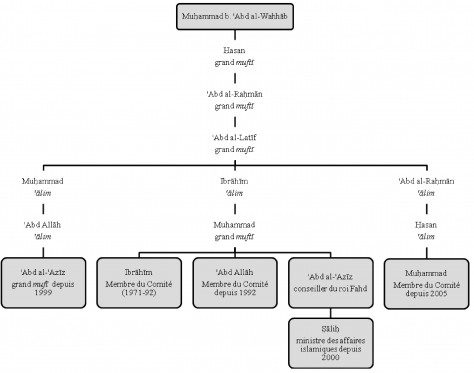
\includegraphics[width=\textwidth]{CourantsIslamContemporain/ImagesCourantsIslamContemporain/genealogie.jpeg}

13 Reste à signaler le cas particulier des oulémas originaires du Hijâz
et d'al-Aḥsā', provinces connues pour leur organisation hétéroclite. En
effet, la plupart des membres du Comité des grands oulémas, originaires
de ces régions, sont issus de ce qu'on a appelé des «dynasties»
d'oulémas, \emph{buyūtāt `ilm}, ou maisons de savoir comme ils aiment
eux-mêmes se faire appeler (à l'instar des familles d'oulémas dans les
autres pays arabes). Plus important encore est le fait que les familles
de ces oulémas appartiennent aux quatre écoles juridiques du sunnisme.
Si le facteur familial revêt une importance certaine, le paramètre de
l'origine tribale doit aussi être pris en compte.
\end{quote}

\hypertarget{la-pruxe9dominance-du-croissant-najdux12b}{%
\section{\texorpdfstring{La prédominance du croissant
\emph{najdī}}{La prédominance du croissant najdī}}\label{la-pruxe9dominance-du-croissant-najdux12b}}

\begin{quote}
14 Force est de constater que l'appartenance à une tribu, généralement
réinventée, constitue un critère identitaire important, dans une société
qui commence à peine à s'individualiser: avant d'être citoyen ou sujet,
on appartient d'abord à une tribu. C'est dire l'importance du milieu
tribal en tant que champ de socialisation des individus. La
\emph{`aṣabiyya}, l'esprit de corps tribal, joue un rôle fondamental
dans le statut social et la promotion de l'individu en Arabie Saoudite.

15 Les oulémas d'origine tribale dominent largement le Comité des grands
oulémas (il s'agit des tribus sédentarisées à partir du e siècle). Ils
sont quarante et un sur les cinquante-deux membres qu'a comptés le
Comité, depuis sa création, à être d'origine tribale, soit 79\%. Les
oulémas d'origine tribale se taillent ainsi la part du lion depuis 1971.
Les onze sièges restants sont occupés par des oulémas issus de trois
milieux différents: des membres de la notabilité citadine du Hijâz
(cooptés pour représenter les intérêts de leur région: on essaie de
choisir les plus «wahhabisés» et/ou quiétistes des oulémas du Hijâz),
des étrangers naturalisés (ils sont hanbalo-wahhabites, ont des talents
«exceptionnels» et ont défendu le hanbalo-wahhabisme et l'État) et des
citadins du Najd, sans affiliation tribale ou \emph{ḫaḍīrī}-s (ces
derniers ne doivent, en principe, leur ascension sociale qu'à leurs
compétences personnelles).

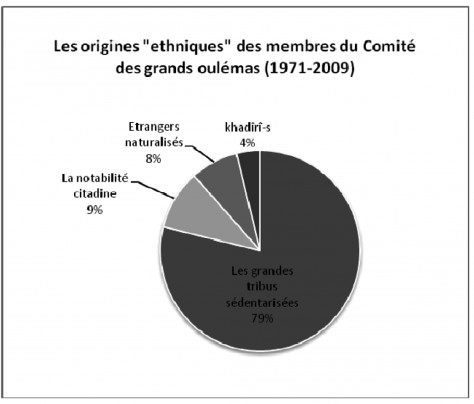
\includegraphics[width=4.9375in,height=4.20833in]{Image/media/image10.jpeg}

16 On constate alors, chiffres à l'appui, que l'appartenance au milieu
tribal sédentarisé joue un rôle déterminant dans l'ascension sociale des
oulémas, la \emph{`aṣabiyya} étant une valeur ajoutée qui permet de se
constituer un capital social. Cela dit, bien que les tribaux dominent
largement en nombre le Comité des grands oulémas, ils ne sont

toutefois pas représentatifs du paysage tribal saoudien. En effet,
certaines tribus comme les Banū Tamīm, les Banū Zayd et les Banū Ḫālid
sont «surreprésentées», tandis que d'autres comme les `Utayba n'ont
guère droit, malgré leur importance numérique, qu'à un seul représentant
au Comité des grands oulémas. D'autres tribus enfin, comme les Šammar,
les Ḥarb, les Muṭayr, les `Ajmān, les Ġāmid, etc. n'ont aucun
représentant au sein du Comité. Si la marginalisation des Šammar, des
`Utayba et des Muṭayr peut s'expliquer par leur passé de tribus
frondeuses, la marginalisation des autres tribus ne peut, elle, être due
qu'à des facteurs religieux et surtout régionaux. Nous nuancerons
seulement, pour finir, en précisant que, dans certains cas, le charisme
personnel du \emph{`ālim} -- c'est le cas d'Ibn Bāz -- fait «oublier»
son appartenance tribale. En effet, ce \emph{`ālim}, citadin sans
affiliation tribale, a pu grimper jusqu'au sommet de l'establishment
hanbalo-wahhabite (il devient grand mufti et président du Comité des
grands oulémas en 1993), uniquement grâce à son «érudition», à son
intégrité morale et à son dévouement aux Sa‛ūd. Le charisme et le
pouvoir symbolique d'Ibn Bāz ont fait de lui le plus grand \emph{`ālim}
hanbalo-wahhabite contemporain.

17 Le royaume d'Arabie Saoudite est un royaume \emph{najdī}. Les élites
saoudiennes sont majoritairement originaires de la région de Najd, fief
de la dynastie et de la doctrine hanbalo-wahhabite. Des études plus
récentes (datant de la dernière décennie) se fondent sur des données
chiffrées mais ne portent que sur les élites ministérielles, la haute
fonction publique et les membres du Conseil consultatif. Rien donc sur
les oulémas. Nous tenterons, dans ce qui suit, de combler ce manque. Sur
les cinquante- deux membres du Comité depuis sa création en 1971, 73\%
des oulémas sont originaires du Najd; 9\% du Ḥijāz, 6\% du Sud, 4\% de
la région orientale et 7\% d'origine étrangère.

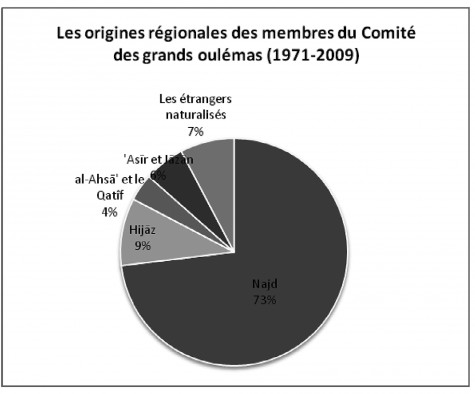
\includegraphics[width=4.94996in,height=4.10417in]{Image/media/image11.jpeg}

18 Une majorité des membres du Comité des grands oulémas est donc
\emph{najdī} et ce depuis sa création. Deux remarques pourraient être
faites à ce propos. La première est que si l'on peut aisément comprendre
que seuls 4\% des grands oulémas sont des Aḥsā'ī-s puisque une grande
partie de la population de cette province est chiite ou sunnite autres
que hanbalo-wahhabite; si l'on peut aussi comprendre que seuls 9\% des
grands oulémas sont \emph{ḥijāzī} puisque, bien que sunnites, ils ne
sont, généralement, pas hanbalo- wahhabites, le chiffre de 6\% seulement
d'oulémas originaires du Sud de l'Arabie Saoudite peut, du moins \emph{a
priori}, paraître absurde puisque les habitants de cette région sont en
majorité hanbalo-wahhabites. L'hypothèse de la préférence régionale peut
être ainsi raisonnablement soutenue: si 73\% des grands oulémas sont
\emph{najdī}, c'est, justement, parce qu'ils sont originaires du fief du
hanbalo-wahhabisme et de la maison
des Sa‛ūd et que, de ce fait, leur soumission à l'un et à l'autre ne
peut être remise en cause. La seconde remarque est que si l'on compare
les chiffres avancés pour le Comité des grands oulémas à ceux que
présente le conseil des ministres au sein duquel les Najdī constituent
72\% des membres (Ibn Ṣunaytān, 2004: 70-73); à ceux du Conseil
consultatif où les Najdī sont majoritaires à 51\% (\emph{ibid}.: 93-96);
à ceux des ministres plénipotentiaires qui sont à 78\% originaires du
Najd ou encore, à ceux des hauts fonctionnaires qui comptent 67\% de
Najdī (\emph{ibid}.: 177-178), on voit que l'élite saoudienne étatique,
qu'elle soit religieuse ou politique, est majoritairement \emph{najdī}.
Les gens du Sud, eux, qui, comme on l'a dit, sont majoritairement
hanbalo-wahhabites, ne représentent que 1\% des ministres, 7\% des
membres de Conseil consultatif, moins de 5\% des ministres
plénipotentiaires et moins de 9\% des hauts fonctionnaires
(\emph{ibid}.: 177- 178): le même raisonnement peut être, ici,
développé. Le régionalisme primerait en Arabie Saoudite. Même si l'on
parle de saoudisation et de formalisation, l'État continue toujours de
s'appuyer sur l'élément najdo-wahhabite pour fonctionner.

19 Observons les chiffres de plus près: lorsque 9\% seulement des
oulémas sont originaires du Hijâz, 20\% des membres du conseil des
ministres, 29\% des membres du Conseil consultatif, 22\% des hauts
fonctionnaires sont \emph{ḥijāzī} (et 34\% parmi eux des cadres
supérieurs). Par ailleurs, en observant les chiffres de plus près
encore, il apparaît qu'au moment de la création du Comité, 29\% des
oulémas sont originaires du Hijâz contre 9\%, nous l'avons dit,
aujourd'hui. Le Comité tend donc, au fur et à mesure qu'il se met en
place et qu'il n'a plus besoin de cadres supérieurs, à se fermer à tout
ce qui n'est pas \emph{najdī}. Il faut ajouter à cela que les oulémas,
quand ils ne sont pas hanbalo- wahhabites, dissimulent leurs croyances
-- ou du moins évitent d'en parler -- et ne jouent, une fois admis au
sein du Comité, qu'un rôle de «figurants».

20 Le Comité des grands oulémas voudrait donner une illusion
d'ouverture: les principales régions sont toutes, même à une faible
proportion, «représentées». Actuellement, deux oulémas d'origine
\emph{ḥijāzi}, deux oulémas originaires du Sud et un autre de l'Est sont
membres du Comité des grands oulémas. En réalité, l'élément \emph{najdī}
domine toujours le Comité, et de loin; de plus, en supposant qu'il y ait
ouverture et même si le Comité accepte en son sein des chiites, il lui
suffirait de conserver une majorité de 51\% de hanbalo-wahhabites
(Najdī) pour que le vote à la majorité absolue passe au sein du Comité
et qu'ainsi, la vision hanbalo-wahhabite continue à dominer.

21 Enfin, en ce qui concerne les oulémas d'origine étrangère, ils ne
sont admis au sein du Comité (au nombre de trois) qu'au moment de la
création de ce Comité. Ces oulémas étrangers étaient, en effet, plus
compétents et plus qualifiés que les oulémas locaux; ils étaient dévoués
à l'État et au hanbalo-wahhabisme; nés non-wahhabites, ils l'étaient
devenus par conviction; ils n'avaient pas d'assise sociale et tribale en
Arabie Saoudite et devaient leur ascension à l'État; enfin, la
solidarité islamique, initiée par le roi Fayçal, entrait également en
ligne de compte. Depuis, le Comité s'est fermé aux étrangers et même les
enfants des dits oulémas étrangers ne sont pas admis au sein du Comité.

22 Le tracé reliant les villes du Najd dont les grands oulémas sont
originaires forme,
pour ainsi dire, un croissant que nous conviendrons d'appeler «croissant
\emph{najdī}» et qui constitue l'épicentre de l'Arabie Saoudite en même
temps que celui du hanbalo- wahhabisme. Il ne faut toutefois pas croire
que si les oulémas du Najd sont largement majoritaires au sein du
Comité, toutes les villes et les régions du Najd y seront équitablement
«représentées». Le Najd compte trois principales régions: la région de
Riyad qui a donné vingt-sept oulémas, le Qaṣīm dix et le Ḥā'il qui n'a
donné aucun \emph{`ālim}. Les deux régions, de Riyad et du Qaṣīm,
offrent un quasi-équilibre dans la répartition des oulémas: dans la
région de Riyad, en dehors de la ville elle-même, qui donne, à elle
seule, sept oulémas, les autres villes donnent, chacune, entre un et
quatre oulémas. De même, dans la région du Qaṣīm, le nombre d'oulémas
par ville varie entre un et trois.

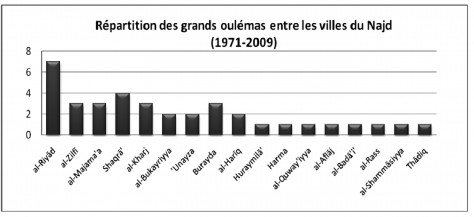
\includegraphics[width=4.9375in,height=2.26042in]{Image/media/image12.jpeg}

23 Le Ḥā'il, quant à lui, est volontairement marginalisé pour une raison
historique évidente: l'émirat du Ḥā'il a longtemps été le rival direct
des Saoud. Nous retrouvons à peine un représentant de cette région dans
le conseil des ministres et un seul autre au Conseil consultatif (Ibn
Ṣunaytān, 2004: 71 et 94).

24 Notons, pour finir, que certaines régions du Najd sont totalement
exclues et n'ont donné aucun \emph{`ālim}: l'exemple d'al-Dawādimī, pour
ne citer que lui, explique ce phénomène dans la mesure où la plupart des
habitants de la ville sont issus de la tribu des `Utayba dont la
fidélité au régime est douteuse. Il y aurait ainsi sous-régionalisation
à l'intérieur même de la régionalisation. De même, aucun grand
\emph{`ālim} n'est issu des régions du Nord. Enfin, aucun chiite n'est
admis au Comité des grands oulémas et ce, pour des raisons évidentes
qu'il ne semble pas utile de rappeler ici. Cela dit, les acquis familial
et tribal, seuls, ne suffisent pas: l'apprenti grand \emph{`ālim} doit
encore suivre un cursus d'études particulier pour intégrer le Comité.
\end{quote}

\hypertarget{de-la-ijux101za-au-doctorat-institutionnalisation-de-la-formation-du-ux101lim}{%
\section{\texorpdfstring{De la \emph{ijāza} au doctorat,
institutionnalisation de la formation du
‛ālim}{De la ijāza au doctorat, institutionnalisation de la formation du ‛ālim}}\label{de-la-ijux101za-au-doctorat-institutionnalisation-de-la-formation-du-ux101lim}}

\begin{quote}
25 Sur les cinquante-deux oulémas qui ont été membres du Comité des
grands oulémas depuis sa création, en 1971, 22\% (soit treize oulémas)
ont reçu une formation traditionnelle et 78\% (soit trente-neuf oulémas)
une formation «moderne». Près d'un quart des oulémas sont ainsi passés
par un cursus traditionnel. Nos entretiens nous permettent de décrire ce
\emph{ta‛līm} et d'en ressortir avec le cursus traditionnel «idéal
typique» du \emph{`ālim} hanbalo-wahhabite.

26 Au départ, entre l'âge de cinq et sept ans, l'apprenti \emph{`ālim}
fait son apprentissage du Coran. Les apprentis oulémas issus d'un milieu
modeste, ceux qui seront plus tard des self-made-men, apprennent le
Coran dans une école coranique (\emph{al-kuttāb}), aux mains d'un cheikh
de renommée moyenne. Les enfants des «cadres religieux moyens» et les
rejetons des dynasties d'oulémas, eux, apprennent le Coran auprès de
leur père, de l'un des membres de leur famille, ou d'un précepteur. On
imagine bien les difficultés rencontrées par les apprentis grands
oulémas issus de milieux modestes et le décalage qui se marque, dès le
départ, entre les apprentis oulémas issus des différentes classes
sociales.

27 Après cette phase d'apprentissage du Coran, l'apprenti \emph{`ālim}
doit, d'une part, commencer à étudier la grammaire et la rhétorique
arabes, de l'autre, apprendre par cœur les trois principaux ouvrages
d'Ibn `Abd al-Wahhāb sur l'unicité divine (\emph{al- tawḥīd}),
fondements du hanbalo-wahhabisme.

28 La troisième étape du cursus classique de l'apprenti \emph{`ālim} est
la quête du savoir
auprès des oulémas réputés. Le futur grand `ālim doit, en effet, réunir
un grand nombre de \emph{ijāzāt} (pl. de \emph{ijāza}: licences), dans
toutes les branches du savoir islamique disponibles, notamment en droit
et en théologie. Il assiste, pour ce faire, plus ou moins
assidûment, à des \emph{ḥalaqāt} `\emph{ilmiyya} ou cercles de savoir,
organisés quotidiennement dans les mosquées ou aux domiciles des
oulémas. Il s'agit alors, de séances de lectures mécaniques suivies de
commentaires d'ouvrages de hadith, d'exégèse coranique, de droit et de
théologie, notamment l'étude des œuvres classiques hanbalites. C'est à
l'issue de ces \emph{ḥalaqāt}, et une fois que l'étudiant a bien retenu
l'ensemble de l'enseignement dispensé par le \emph{`ālim}, qu'il fait un
\emph{istid`ā'}: une demande d'\emph{ijāza} pour les ouvrages étudiés.
Les étudiants les plus brillants deviennent assistants du maître et cela
leur ouvre la porte pour devenir professeur ou juge: la carrière est
alors lancée. Cela a été le cas de Muḥammad al-Sbayyil, le dernier grand
\emph{`ālim} à avoir reçu une formation traditionnelle.

29 Né dans la région du Qaṣīm vers 1926, al-Sbayyil est issu d'une
famille de «cadres religieux moyens». Son père, libraire et copiste
d'ouvrages religieux, connaît parfaitement le Coran. Son frère aîné,
`Abd al-`Azīz, est un \emph{`ālim} de la ville d'al- Bukayriyya. À l'âge
de cinq ans, al-Sbayyil commence son apprentissage du Coran auprès de
son père puis de son frère. Vers l'âge de dix ans, il se lance dans
l'apprentissage des trois ouvrages fondamentaux d'Ibn `Abd al-Wahhāb. Il
étudie aussi la jurisprudence hanbalite sous la direction des oulémas du
Qaṣīm, notamment les ouvrages d'Ibn Taymiyya (m. 1328), d'Ibn Qayyim
al-Jawziyya (m. 1350) et de Mar`ī al- Karamī (m. 1624), etc. À l'âge de
vingt ans, il aurait déjà acquis plusieurs \emph{ijāzāt} qui lui
permirent de devenir l'assistant du juge du Qaṣīm, `Abd Allāh b. Ḥumayd.

30 La formation traditionnelle indispensable au tout début du e siècle
perd, peu à peu, du terrain. En effet, les oulémas qui ont reçu cette
formation s'adaptent difficilement aux exigences de la modernité. 53\%
des membres du Comité des grands oulémas, soit neuf oulémas, ont reçu,
en 1971, une formation dite traditionnelle; en 2009, aucun grand
\emph{`ālim} ne bénéficie d'une telle formation. Dans un pays qui tente
de se moderniser, le besoin d'uniformisation de la formation des grands
oulémas s'impose. Il a fallu, pour y répondre, créer un cursus complet,
homogène, un cursus «national». Nous entendons par cursus moderne, un
cursus «institutionnalisé» et uniformisé.

31 S'ils ne sont que 47\% (soit huit oulémas), en 1971, à suivre la
formation dite moderne,

ils sont aujourd'hui 100\% à le faire. Après un cycle d'études primaires
dans des écoles publiques2\emph{,} les élèves qui se destinent à faire
une carrière juridico-religieuse, rejoignent les instituts de sciences
religieuses (\emph{al-ma`āhid al-`ilmiyya}). Le premier institut voit le
jour à Riyad, en 1950, à l'instigation du grand mufti du royaume de
l'époque, Muḥammad b. Ibrāhīm. Mais très vite, le gouvernement adopte le
projet et les instituts fleurissent dans toutes les régions du royaume
pour atteindre le chiffre de soixante- deux en 2009. Pour accéder à
l'enseignement de ces instituts, l'enfant doit avoir un dossier correct
et avoir appris au moins deux parties du Coran. L'enseignement y est
gratuit. Les instituts de sciences religieuses proposent un cursus de
six années: trois années de collège sanctionnées par un certificat de
réussite, sorte de «brevet» et trois années de lycée sanctionnées par un
certificat de réussite, sorte de «baccalauréat». Les matières étudiées
ont évolué depuis les années cinquante. Au début, l'enseignement était
constitué de quatre troncs communs: les sciences religieuses, les
sciences de la langue arabe, les «sciences sociales», et les
mathématiques. Au fil des années, on a ajouté à ce tronc commun d'études
de base, l'apprentissage obligatoire de la langue anglaise et de
l'informatique. Ces instituts de sciences religieuses sont inégalement
répartis sur l'ensemble du pays: le Najd compte 34\% des instituts, le
Hijâz 13\%, le Sud 28\%, le Nord 18\%, l'Est, enfin, 7\%. Les instituts
sont nombreux dans les régions où le hanbalo-wahhabisme est majoritaire
c'est-à-dire dans le Najd, le Sud et le Nord.

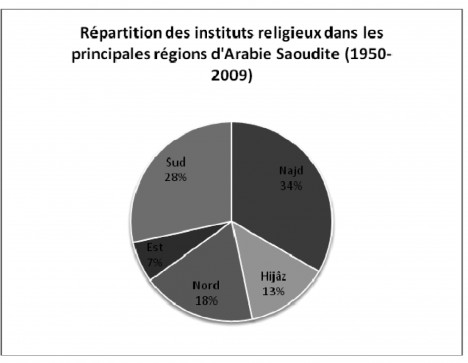
\includegraphics[width=4.875in,height=3.78125in]{Image/media/image13.jpeg}

32 Si la proportion entre le nombre d'instituts créés dans le Hijâz et
celui des oulémas qui sont admis au Comité des grands oulémas est
relativement équilibrée, la proportion entre le nombre d'instituts créés
dans les trois autres régions hanbalo-wahhabites et celui des oulémas
issus de ces régions et effectivement admis au sein du Comité, est,
quant à elle, largement déséquilibrée. On s'attendrait, en effet, à un
nombre plus important d'instituts de sciences religieuses dans le Najd,
à un nombre moins important dans le Sud et à un nombre nul d'instituts
dans la région du Nord. Or, ils sont créés dans le Nord et dans le Sud
mais ce, moins dans le but de former des grands oulémas que dans celui
de «wahhabiser» ces régions en y formant des techniciens du culte
hanbalo-wahhabite et des «cadres religieux moyens».

33 Lorsque l'apprenti \emph{`ālim} a terminé avec succès ses études
secondaires au sein de l'institut, il peut postuler pour les trois
grandes universités du pays: l'Université islamique de Médine (al-Jāmi`a
al-islāmiyya), l'Université islamique de la Mecque (Jāmi`at Umm al-Qurā)
et l'Université islamique de Riyad (Jāmi`at al-imām Muḥammad b. Sa`ūd
al-islāmiyya).

34 La première de ces universités, fondée en 1961, accueille surtout les
musulmans étrangers. Les Saoudiens qui y étudient se destinent
généralement à la prédication à l'étranger. De cette université n'est
issu qu'un seul grand \emph{`ālim}.

35 Quant à la deuxième citée, elle est la plus ancienne université de
théologie d'Arabie Saoudite, fondée en 1949. Elle n'a, malgré son
ancienneté, donnée que six grands oulémas. Doit-on y voir une
manifestation du régionalisme saoudien? Toujours est-il que cette
université accueille, depuis les années soixante-dix, des professeurs,
des cadres et des étudiants de diverses tendances politico-religieuses,
notamment des frères musulmans et des sahwistes (Lacroix, 2010: 47-97)
en lesquels le gouvernement saoudien et le Comité des grands oulémas
n'ont que très peu confiance et qui ne sont donc pas spontanément
recrutés par celui-ci.

36 La dernière université, enfin, est incontestablement la plus
importante pour notre étude. Elle a donné vingt-cinq oulémas, soit 51\%
des membres du Comité, depuis sa création en 1971, et 75\% des oulémas
ayant fait des études universitaires modernes. Cette université naît, en
1974, de la fusion de la faculté de théologie créée, elle, en 1953, et
de la faculté de langue arabe, créée en 1954.

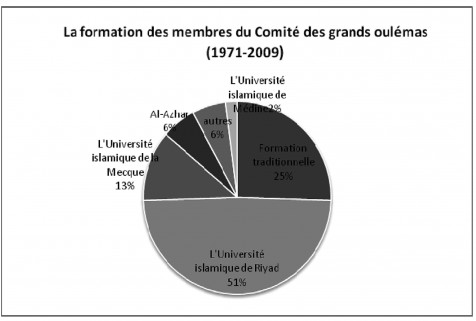
\includegraphics[width=4.95833in,height=3.34375in]{Image/media/image14.jpeg}

37 Depuis sa création, l'Université islamique de Riyad, qui,
rappelons-le, porte le nom du fondateur de l'émirat saoudien Muḥammad b.
Sa`ūd (1744-1765), fidèle allié d'Ibn `Abd al-Wahhāb, est considérée
comme le vivier des grands oulémas et de tous les cadres religieux et
techniciens du culte dont l'establishment religieux a besoin. Le

«pharaonique» campus de l'université (une véritable ville dans la ville
avec ses propres infrastructures, un petit hôpital, un supermarché, des
quartiers résidentiels pour les étudiants, les professeurs et le
personnel administratif, etc.) compte neuf facultés et deux instituts
supérieurs: la faculté de droit {[}musulman{]}; la faculté de théologie;
la faculté de langue arabe; la faculté des sciences sociales
{[}islamiques{]}; la faculté de la prédication et de la communication;
la faculté des langues et de la traduction; la faculté des sciences de
l'informatique; la faculté de l'économie; la faculté des sciences;
l'Institut supérieur de la magistrature et l'Institut de l'apprentissage
de la langue arabe {[}pour les étrangers{]}. Cela dit, les grands
oulémas sont exclusivement issus des facultés de droit et de théologie
et de l'Institut supérieur de la magistrature. Les étudiants dans ces
trois domaines bénéficient d'une bourse d'études et obtiennent, dès la
fin de leur première année d'études, le titre fort apprécié de
\emph{shaykh}. Le succès de l'Université islamique de Riyad est tel que
celle-ci s'est engagée dans une politique d'expansion en développant
deux filiales en Arabie Saoudite3 et cinq à l'étranger4\emph{.} Enfin,
certains étudiants peuvent préparer leur doctorat en sciences
religieuses à l'université égyptienne d'al-Azhar, pour le prestige que
cela donne. Une autre raison pourrait être avancée: certains apprentis
oulémas saoudiens iraient à al-Azhar pour observer l'organisation, les
structures et les mécanismes de fonctionnement de cette prestigieuse
université en vue de les
«importer» en Arabie Saoudite.

38 Les oulémas, au moment de leurs études supérieures, ont tous un tronc
commun tripartite: les fondements de la théologie (\emph{al-`aqīda});
l'exégèse coranique (\emph{al tafsīr}) et la jurisprudence
(\emph{al-fiqh}). À partir de la première année de master (calqué sur le
système anglo-saxon), 74\% des oulémas se spécialisent dans la
jurisprudence, et plus spécialement dans les fondements de la
jurisprudence islamique (\emph{uṣūl al-fiqh}) dans le but d'acquérir la
qualification requise pour émettre des \emph{fatwā}; 26\% d'entre eux,
se spécialisent en théologie, et plus précisément en religions comparées
(en réalité, pour dénigrer toute autre religion que l'islam
hanbalo-wahhabite)5\emph{.} Le choix de ces spécialisations n'est pas
étonnant dans la mesure où les étudiants se destinent avant tout à être
des techniciens du culte et des gestionnaires des biens de salut. Nous
n'entrerons pas, pour ne pas alourdir notre propos, dans le détail des
spécialisations pointues à l'intérieur même des deux grands domaines de
spécialisations que nous avons évoqués.

39 Bien que le cursus moderne se soit bien implanté dans le paysage
saoudien, l'ijāza
n'en demeure pas moins source de prestige et un élément non négligeable
dans un
capital social. Nous avons pu observer que la totalité des oulémas qui
ont suivi le cursus moderne ont, néanmoins, obtenu une ou plusieurs
\emph{ijāzāt}. Elément de prestige comme nous venons de le dire,
l'\emph{ijāza} est, en théorie, facultative. Mais, en pratique,
l'obtention d'une \emph{ijāza} permet au \emph{`ālim}, d'une part, de se
rattacher à une chaîne de transmission
«ininterrompue» d'oulémas remontant jusqu'au Prophète, ce qui permet au
\emph{`ālim} de légitimer sa position et son savoir et de s'inscrire
dans l'héritage prophétique, d'autre part, de nouer des relations
privilégiées avec un ou plusieurs oulémas et de commencer ainsi à tisser
un réseau qui pourra le mener au sommet de l'establishment hanbalo-
wahhabite.

\textbf{Faire carrière: le \emph{cursus honorum} des oulémas}

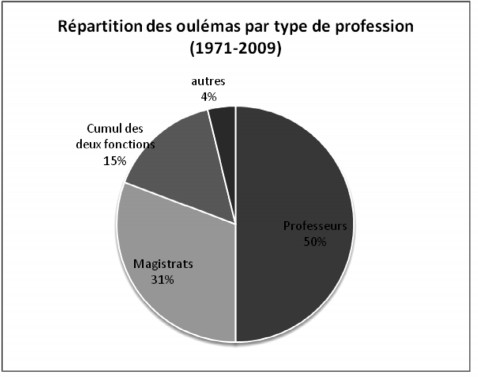
\includegraphics[width=4.97917in,height=3.92708in]{Image/media/image15.jpeg}40
L'enseignement et la magistrature ont toujours été les métiers de
prédilection des oulémas. Les membres du Comité des grands oulémas
n'échappent pas à cette règle. 96\% d'entre eux exercent au moins une de
ces deux professions: 50\% du Comité, soit vingt et un grands oulémas,
ont été ou sont encore, professeurs de jurisprudence islamique ou de
théologie; 31\% d'entre eux sont magistrats dans les différentes
instances de la justice saoudienne; 15\% des grands oulémas ont cumulé
les deux fonctions. À la question: «pourquoi le choix de ces métiers?»
Une première réponse, unanime, des grands oulémas magistrats: «la
justice est le fondement de la royauté». Et, selon les oulémas, qui,
mieux que des spécialistes de «la loi divine», pourraient mettre la
justice en application! Les grands oulémas ont d'ailleurs pleine
conscience de l'importance de leur mission. Ils ont une vision
catastrophiste d'un monde où le \emph{`ilm}, qui risque d'être perdu,
doit être sauvé, épuré des innovations blâmables et transmis par le
\emph{`ālim}.

41 En outre, si la magistrature permet au grand \emph{`ālim} d'observer,
d'analyser et de statuer sur des cas concrets, l'enseignement permet de
transmettre le savoir théorique. Cela, en plus du prestige qui entoure
ces deux fonctions. Il n'est, enfin, pas étonnant de voir que nombre de
grands oulémas cumulent les deux fonctions puisqu'en réalité, l'une et
l'autre sont indissociables (pratique et théorie). Ce phénomène de cumul
des fonctions (d'enseignant et de magistrat) est surtout visible dans la
première génération des grands oulémas. Il s'explique par le manque de
cadres religieux au moment de la
création du Comité. Les grands oulémas devaient donc assumer, tout à la
fois, leur rôle au sein du Comité et les fonctions de magistrats et
d'enseignants. Des années quarante aux années soixante, l'Arabie
Saoudite a été obligée d'«importer» des cadres religieux de l'étranger,
notamment de l'Égypte. Un exemple: l'Égyptien `Abd al-Razzāq `Afīfī (m.
1994), arrivé en Arabie Saoudite, en 1949, pour enseigner la langue
arabe et les sciences religieuses dans un collège à Tayef, a gravi, un à
un, les échelons et parvient au sommet de l'establishment religieux: il
est nommé, en 1971, au sein du Comité des grands oulémas. Cet exemple
révèle deux réalités: premièrement, l'Arabie Saoudite a fait appel aux
étrangers pour l'enseignement, à une certaine époque, à cause du déficit
de cadres dont elle a souffert dans tous les domaines; et deuxièmement,
les étrangers hanbalo-wahhabites, qui pouvaient aisément s'intégrer dans
le pays d'accueil, ont pu, à force de persévérance, atteindre le sommet
de l'establishment religieux saoudien.

42 La pratique du cumul des fonctions d'enseignant et de magistrat tend
à disparaître: le dernier grand \emph{`ālim} à avoir cumulé ces deux
fonctions est `Abd Allāh b. Qa`ūd, membre du Comité de 1977 à
19866\emph{.} Désormais, les grands oulémas, qu'ils soient professeurs
ou magistrats, sont de plus en plus spécialisés, chacun dans son
domaine: de professeurs de droit en général, ils sont devenus
professeurs de droit pénal, de droit de la famille, etc. Parallèlement à
ces deux métiers de prédilection, les grands oulémas sont techniciens du
culte: la plupart d'entre eux sont imâm dans les mosquées. Par exemple,
le grand mufti actuel du royaume, `Abd al-`Azīz āl al-Shaykh, est
également imâm de la grande mosquée de Riyad. Sāliḥ b. Ḥumayd est, lui,
imâm de la grande mosquée de la Mecque, etc. N'oublions pas enfin,
l'autre fonction essentielle des grands oulémas, celle d'«entrepreneurs»
de biens de salut, à savoir promulguer des \emph{fatwā} et se mettre à
l'écoute de la population. Mais si les grands oulémas monopolisent les
grands postes religieux et judiciaires saoudiens, ils n'hésitent pas à
empiéter sur le domaine réservé des autres élites.

43 Une fois admis au sein du Comité, le grand \emph{`ālim} obtient
automatiquement le grade de haut fonctionnaire (\emph{al-martaba
al-mumtāza}), voire celui de ministre. Sur les cinquante-deux membres du
Comité des grands oulémas, vingt-deux ont occupé des postes de
responsabilité autres que ceux de magistrats et d'enseignants. Déjà neuf
membres de la \emph{Hay'a} ont été ou sont encore ministres. Les
ministères que contrôlent les oulémas (si ce ne sont pas eux qui les
contrôlent directement, c'est un membre de l'establishment religieux)
sont ceux de la justice, des affaires islamiques, du pèlerinage et de
l'enseignement des filles (avant le rattachement de ce dernier, en 2002,
au ministère de l'éducation nationale). Depuis sa création, le ministère
de la justice est dirigé par un membre du Comité7\emph{.} Huit membres
du Comité des grands oulémas on été membres du Conseil consultatif: le
président de ce conseil, qui fait se côtoyer islamistes,
«libéraux», conservateurs et tribaux, depuis sa création, en 1992, est
un membre du Comité des grands oulémas. De 1992 à 2002, c'est Muḥammad
b. Jubayr, membre du Comité des grands oulémas (de 1971 à 2002), qui
assure la présidence de cette instance. Sāliḥ b. Ḥumayd, membre du
Comité des grands oulémas depuis 2001, lui succède en 2002. Ce dernier
est remplacé par `Abd Allāh Āl al-Shaykh, en 2009. Trois membres de la
\emph{Hay'a} ont été conseillers du roi Fahd (1982-2005) et deux sont
actuellement conseillers du roi `Abd Allāh. Quatre membres du Comité ont
occupé les postes de doyen ou de président d'université. Par exemple,
`Abd al-`Azīz b. Bāz occupe jusqu'à sa mort, en 1999, le poste de
président de l'Université islamique de Médine. Sa`d al- Ḍuwayḥī est
doyen de la faculté de théologie d'al-Aḥsā'. `Abd Allāh b. `Abd
al-Muḥsin al- Turkī, sans doute l'un des membres les plus actifs du
Comité, actuellement, occupe le poste de président de la Ligue islamique
mondiale, après avoir occupé, entre autres, les postes de président de
l'Université de Riyad et de ministre des affaires islamiques.

44 C'est dire que les oulémas ont adopté, depuis au moins deux
décennies, une stratégie adaptative qui les pousse à investir plusieurs
secteurs d'activités. Outre les domaines religieux, législatif et
éducatif, ils investissent les associations caritatives, les
organisations gouvernementales et non gouvernementales et les domaines
économique et financier. Dans ces deux derniers domaines, trois oulémas,
`Abd Allāh b. Manī`, `Abd
al-Wahhāb Abu Sulaymān et `Abd Allāh al-Muṭlaq se sont «improvisés»
experts et consultants incontournables dans les marchés financiers
saoudiens. Les trois hommes sont aussi membres de plusieurs conseils
d'administration de banques et d'entreprises dans le cadre de ce que
l'on appelle en Arabie Saoudite \emph{al-lijān al-šar`iyya} ou
commissions islamiques. Le nom-même d'un grand \emph{`ālim} sur la
brochure d'une société ou d'une entreprise est la meilleure des
publicités.
\end{quote}

\hypertarget{la-multiplication-des-ruxe9seaux-de-soutien}{%
\section{La multiplication des réseaux de
soutien}\label{la-multiplication-des-ruxe9seaux-de-soutien}}

\begin{quote}
45 Cette mobilité des oulémas n'est, toutefois, possible que si le
\emph{`ālim} tisse, autour de lui, un réseau sur lequel il peut
s'appuyer. Les capitaux culturel et économique doivent encore être
complétés par un réseau de soutiens. Nous avons pu observer trois types
de capitaux sociaux mobilisés par le futur grand \emph{`ālim}. Autrement
dit, le recours aux relations personnelles permet à ce dernier de
s'assurer une meilleure position dans la hiérarchie sociale. Ces trois
réseaux, que nous exposons séparément, sont en réalité, presque
toujours, combinés par le futur grand \emph{`ālim}. Le réseau familial
constitue la première ressource du futur grand \emph{`ālim}. Nous avons,
en effet, constaté l'existence d'au moins trois exemples de réseaux
familiaux qui sont autant de moyens d'accès au Comité des grands
oulémas.

46 Le premier est, sans aucun doute, le plus puissant et le plus dense:
celui des Āl al- Shaykh. Nous avons évoqué plus haut l'importance de
cette famille et nous tenterons, dans ce qui suit, de compléter le
tableau amorcé. L'exemple des deux fils, Ibrāhīm et `Abd Allāh, du grand
mufti Muḥammad b. Ibrāhīm est tout à fait significatif: bien que le
premier des deux ait été relativement peu brillant par rapport aux
collaborateurs de son père, il a quand même été nommé par ce dernier
vice-mufti du royaume d'Arabie Saoudite. Après la mort de son père et la
suppression du poste de mufti, Ibrāhīm, qui était destiné à devenir
mufti, reçoit, en guise de consolation, les postes de ministre de la
justice, de membre du Comité des grands oulémas et de président de la
Direction de la recherche scientifique, de la prédication et de
l'instruction! En 1992, lorsqu'Ibrāhīm se retire des affaires, son
remplaçant au ministère et au Comité des grands oulémas n'est autre que
son frère cadet `Abd Allāh, président actuel du Conseil consultatif. Un
autre exemple étonnant de la famille Āl al-Shaykh: il s'agit de Ṣāliḥ b.
'Abd al-`Azīz, le petit fils d'Ibn Ibrāhīm. Après avoir fait des études
scientifiques depuis le lycée et obtenu un diplôme d'ingénieur, Ṣāliḥ
décide de récupérer l'héritage familial et s'inscrit à l'Université
islamique de Riyad. Grâce à son nom et à l'intervention de son père, qui
était l'un des conseillers du roi Fahd, il obtient une équivalence et
passe ainsi directement en année de master: il contourne la règle qui,
aussi stricte soit-elle, s'efface quand il s'agit d'un Āl al-Shaykh. Il
est actuellement ministre des affaires islamiques et, potentiellement,
membre du Comité des grands oulémas. Un dernier exemple enfin de cette
famille: le dernier admis à Hay'at kibār al-'ulamā', Muḥammad b. Ḥasan,
fait une ascension fulgurante grâce à ses bonnes relations avec son
cousin, le grand mufti actuel d'Arabie Saoudite: il a pu, rapidement,
gravir les échelons universitaires et devenir le directeur de cabinet du
mufti. Ce dernier l'épaule et le soutient: il propose son nom au Comité
des grands oulémas auquel Muḥammad b. Ḥasan accède en avril 2005.
Signalons, enfin, que le réseau familial des Āl al-Shaykh et l'influence
qui en découle, dépassent largement le seul cadre religieux: un membre
de la famille est ambassadeur à Paris, un autre est directeur du
protocole royal, un troisième est membre de la chambre de commerce, etc.
Le deuxième réseau familial est celui des Ibn Ḥumayd, déjà présenté plus
haut.

47 Le dernier réseau familial, enfin, de moindre importance, est celui
des al-Šathrī: cette
famille du Najd a donné quelques oulémas et plusieurs hommes politiques.
`Abd al-‛Azīz al-Šathrī, un des conseillers des rois Fayçal (1964-75) et
Ḫālid (1975-82) a également été un ouléma de renommée moyenne. Son fils,
Nāṣir, a réussi à faire une brillante carrière politique (en tant que
conseiller des rois Ḫālid et Fahd). Selon un des
membres du clan al-Šathrī: «il ne manquait à {[}la{]} famille qu'un
grand \emph{`ālim} pour qu'{[}elle{]} devienne, enfin, une grande
famille». La parentèle met tout en œuvre pour que son rejeton prodige,
Sa‛d, accède au sommet de l'establishment religieux. Aussi, le
prépare-t-on, dès son plus jeune âge, à devenir grand \emph{`ālim} : on
le confie aux maîtres les plus compétents dans le domaine, tels Ibn Bāz,
Ibn `Uthaymīn, al-Aṭram, al-Rakbān et `Abd al-`Azīz Āl al-Shaykh. On le
pousse à s'inscrire à Jāmi'at al-imām où il obtient un doctorat en
fondements de la jurisprudence islamique. Sa`d brûle toutes les étapes
du \emph{cursus honorum} hanbalo-wahhabite et devient professeur de la
même université en un temps records. En mars 2005, la famille soutient
la candidature de son fils au Comité des grands oulémas (le père est
membre du cabinet royal qui transmet les candidatures au roi). Sa`d est
finalement nommé, en avril 2005: à trente-huit ans, il est le plus jeune
membre de l'histoire du Comité des grands oulémas.

48 Nous l'avons dit, le régionalisme et le segmentarisme dominent le
paysage politico- religieux saoudien. La deuxième ressource du futur
grand \emph{`ālim} est, naturellement, le réseau tribal qui va de pair
avec le réseau régional, autrement dit avec le réseau \emph{najdī}. Nous
avons remarqué, en analysant les origines géographiques et tribales des
grands oulémas, que ces derniers sont généralement issus des plus
grandes confédérations tribales du Najd: les Banū Ḫālid ont donné quatre
grands oulémas, les Banū Zayd, sept, les Banū Subay`, trois, les Banū
Tamīm, huit (auxquels il faut ajouter les quatre grands oulémas des Āl
al-Shaykh), les Qaḥṭān, trois, les `Unayza, trois, les Bāhila, deux et
al- Dawāsir, deux également. Soit un total de trente-six grands oulémas
issus des grandes tribus du Najd sur les cinquante-deux membres du
Comité. Le réseau tribal est très dense. Le nombre de grands oulémas est
plus ou moins bien réparti entre les grandes tribus \emph{najdī}. D'un
mouvement de nomination au sein du Comité à l'autre, cet équilibre est,
consciemment ou inconsciemment, maintenu. Exemple: les deux grands
oulémas, Muḥammad āl Sulaymān et Bakr Abū Zayd, de la tribu des Banū
Zayd -- admis tous deux au Comité, en 1992 -- sont remplacés, en 2005,
par deux hommes issus de la même tribu, `Alī al-Ḍuwayḥī et `Abd
al-Raḥmān al-Sadḥān. D'ailleurs, le réseau tribal doublé du réseau
régional ne concerne pas uniquement le champ religieux: on retrouve ces
mêmes configurations dans le domaine politico-administratif (Ibn
Ṣunaytān, 2004, 59-62).

49 La dernière ressource du futur grand \emph{`ālim} est la
\emph{mulāzama}: le fait de s'attacher un
long moment à un maître en sciences religieuses, réputé et influent.
Côtoyer un maître pendant plusieurs années permet à l'apprenti grand
\emph{`ālim} de nouer avec lui des relations personnelles qui peuvent
même aboutir au mariage de l'élève avec la fille ou la nièce du maître.
Par exemple, Ṣāliḥ al-Luḥaydān est, pendant plusieurs années, le
disciple favori du grand mufti Muḥammad b. Ibrāhīm. Cette relation
privilégiée lance véritablement la carrière de Ṣāliḥ qui devient le
gendre et le directeur de cabinet du mufti et qui gagne peu en peu en
charisme. Une année seulement après le décès du maître, al-Luḥaydān est
admis au Comité des grands oulémas; il hérite aussi de la fonction de
magistrat; quelques années plus tard, il devient le président du Haut
conseil de la magistrature, poste qu'il occupe jusqu'en février 2009.
Al-Luḥaydān est le doyen du Comité des grands oulémas dont il est membre
depuis 1971. Il en est aussi un des membres les plus influents. Il
serait, en effet, le seul à pouvoir opposer un veto pour la nomination
d'un nouveau membre: en 2005, il aurait utilisé son veto pour s'opposer
à l'entrée de l'ouléma `Abd al-Muḥsin al-`Ubaykān au Comité.

50 Un autre exemple: Muḥammad al-Sbayyil est le disciple d'Ibn Ḥumayd
alors que
celui-ci est le \emph{qāḍī} d'al-Bukayriyya. Quand Ibn Ḥumayd devient le
\emph{qāḍī} du Qaṣīm, il fait appeler al-Sbayyil à Burayda pour le
désigner professeur et responsable d'un institut de sciences religieuses
de la région. La relation entre les deux hommes est telle que,
lorsqu'Ibn Ḥumayd devient le grand juge du Ḥijāz, il le fait venir à la
Mecque et le nomme imâm de la grande mosquée de la Mecque et
vice-président de l'administration chargée de gérer les deux lieux
saints. Il finit même par en devenir président (jusqu'en 2005) après la
disparition de son protecteur. Depuis son arrivée à la Mecque, il tisse
des
relations étroites avec des oulémas et grands oulémas notamment Ibn Bāz
(qui n'est pas son maître) mais qui finit par lui proposer de devenir
membre du Comité en 1992.

51 Un troisième exemple: c'est également Ibn Bāz qui suit, pas à pas, la
carrière de `Abd
Allāh b. Qa'ūd qui est son meilleur disciple. À la première occasion (le
décès d'Ibn Ḥumayd et de Miḥḍār `Aqīl), Ibn Bāz propose le nom d'Ibn
Qa`ūd au cabinet royal qui le nomme membre du Comité en 1977.

52 Un dernier exemple enfin: le mufti actuel, `Abd al-`Azīz āl
al-Shaykh, en plus du réseau familial que lui confère son nom, bénéficie
du soutien de son maître Ibn Bāz. Il s'agit d'abord d'une question de
solidarité et de reconnaissance: Ibn Bāz est un \emph{mulāzim} du grand
père de `Abd al-`Azīz Āl al-Shaykh, Muḥammad b. `Abd al-Laṭīf. Il aide
donc `Abd al-`Azīz Āl al-Shaykh à devenir professeur à l'université
d'al-Imām, et propose son nom au cabinet royal pour en faire un membre
du Comité des grands oulémas (il le deviendra en 1987). En 1993, Ibn Bāz
devient mufti et désigne `Abd al-`Azīz āl al-Shaykh vice-mufti du
royaume et ce, bien que d'autres grands oulémas soient plus compétents
que lui. En effet, depuis les années soixante et jusqu'à sa mort, en
1999, Ibn Bāz occupe une position-clé dans l'establishment religieux. Il
bénéficie du respect et de la considération des autres grands oulémas et
exerce, de ce fait, une influence autour de lui, tous les grands oulémas
tenant compte de ses conseils et suivant à la lettre ses directives. La
centralité d'Ibn Bāz est ainsi très importante: un grand nombre de
chemins passent par lui. Dix-huit grands oulémas sont ses disciples et
certains d'entre eux lui doivent leur entrée au sein du Comité.
\end{quote}

\hypertarget{le-quiuxe9tisme-politique}{%
\section{Le quiétisme politique}\label{le-quiuxe9tisme-politique}}

\begin{quote}
53 En cherchant à identifier les conditions d'accès au Comité des grands
oulémas à travers le parcours de ses membres, nous avons constaté qu'il
existe deux critères directement liés à la vie politique et sociale:
aucun des grands oulémas n'a de passé politique (c'est-à-dire, une
quelconque manifestation d'opposition au régime: demande de réformes, ou
autres), et aucun \emph{`ālim} n'a jamais critiqué les décisions du
Comité ou de l'un de ses membres et ce, même si ses positions allaient à
l'encontre des décisions officielles.

54 `Abd Allāh Ibn Jibrīn, haut fonctionnaire religieux et candidat
potentiel au Comité des grands oulémas, a été l'un des parrains de la
contestation islamiste des débuts des années quatre-vingt-dix (Kepel,
2003: 335-337; Lacroix, 2007: 371-443). Ces actes constituent une
véritable offense tant pour le régime que pour les grands oulémas. Ces
derniers ne manquent pas, d'ailleurs, de le désavouer publiquement: il
est démis de ses fonctions officielles. Réhabilité par la suite, et bien
que très bon \emph{`ālim}, il ne pourra cependant jamais prétendre au
poste de grand \emph{`ālim} en raison de cette «bavure»: s'étant
ouvertement opposé au gouvernement et ayant participé à des activités
politiques allant à l'encontre des positions officielles, son «rachat»
et son récent soutien au gouvernement ne suffisent pas. Il ressort de
cet exemple que le quiétisme politique des candidats au Comité est un
élément fondamental et un critère-clé de sélection. Tout ce que peut
tolérer le Comité comme engagement politique pour un futur grand
\emph{`ālim} est le soutien aux décisions du pouvoir. `Alī al-Ḍuwayḥī
est l'exemple du \emph{`ālim} engagé politiquement -- en faveur du
régime bien sûr -- qui accède à la Hay'a. En effet, depuis 2001,
al-Ḍuwayḥī, qui dirige la faculté de théologie d'al-Aḥsā', a signé
plusieurs pétitions politiques défendant les programmes scolaires
saoudiens, et se déclarant en faveur de la tenue d'élections
municipales, etc.

55 Quant à `Abd al-Muḥsin al-`Ubaykān, qui a appelé ouvertement le
gouvernement à entreprendre des réformes, entre 1992 et 1994, il a été
marginalisé et démis de ses multiples fonctions: il perd son poste de
juge au tribunal de Riyad et d'imâm de mosquée. Réhabilité, dans les
années 1999-2000, il continue néanmoins à critiquer les décisions de la
Hay'a (surtout celles qui concernent la jurisprudence), et du système
judiciaire. Il émet même des \emph{fatwā} contredisant celles du Comité
des grands oulémas et
tente, pour se rattraper, de promulguer des \emph{fatwā} sur la licéité
du salut du drapeau national, sur la condamnation des sahwistes ou
encore sur l'interdiction du djihâd en Irak pour les Saoudiens. Le
gouvernement a accepté de le réhabiliter mais les oulémas ont opposé un
veto catégorique à l'entrée de ce \emph{`ālim} au Comité. Al-`Ubaykān a,
finalement, été nommé, dans un premier temps, conseiller au ministère de
la justice et membre du Conseil consultatif, avant de devenir l'un des
conseillers du roi, en 2009.

56 Les leaders de la \emph{ṣaḥwa} dans les années quatre-vingt-dix,
Safar al-Ḥawālī, Salmān al-`Awda et Muḥsin al-`Awājī, reconnaissent
eux-mêmes que l'un des critères d'accès au Comité des grands oulémas est
le quiétisme sur les plans politique et sécuritaire et acceptent donc,
du fait de leur très grand engagement politique, de ne pas y prétendre.

«Pour le gouvernement, dit al-Ḥawālī, les grands oulémas doivent être
des hommes apolitiques, des hommes qui ignorent tout de la politique».
Salmān al-`Awda ajoute que

«les futurs membres du Comité doivent être des hommes sans histoire(s)».
Pour Muḥsin al-`Awājī «l'accès au Comité obéit à des critères purement
sécuritaires».

57 Il découle de tout cela le «portrait idéal» du membre du Comité des
grands oulémas:

le grand \emph{`ālim} est hanbalo-wahhabite; il est issu d'une famille
de «cadres religieux moyens» ou d'une «dynastie» d'oulémas; il est issu
d'une grande tribu sédentarisée du croissant \emph{najdī}; il a effectué
des études auprès de maîtres réputés (cela pour le \emph{`ālim} qui suit
une formation traditionnelle) ou dans un \emph{ma`had `ilmī} puis à
l'université al-Imām de Riyad (pour le grand \emph{`ālim} qui a reçu une
formation moderne); il s'est spécialisé en jurisprudence islamique; il
est généralement professeur d'université (al-Imām) ou magistrat; il a en
moyenne vingt-cinq années d'expérience dans le domaine religieux; il
n'est pas engagé politiquement (s'il l'est, il ne doit l'être qu'en
faveur du régime).

58 La moyenne d'âge du grand \emph{`ālim} qui accède au Comité est de
quarante-sept ans. Il y reste en moyenne quinze ans. Et, si les
circonstances d'accès à la Hay'a sont difficiles à déterminer, les
circonstances de départ de la Hay'a sont, elles, tout à fait claires: le
grand \emph{`ālim} quitte le Comité s'il décède, bien évidemment, s'il
est gravement malade ou s'il a commis un acte jugé répréhensible par le
roi -- en 1992, quatre grands oulémas auraient refusé de signer une
\emph{fatwā} et ont été limogés.

59 Le renouvellement des membres du Comité des grands oulémas est
généralement associé à une période de crise ou de transition. Les
renouvellements de 1987 et de 2001 sont des renouvellements de
transition (plusieurs oulémas sont décédés ou gravement malades), les
renouvellements de 1992 et 2005 coïncident avec des moments de crise
(respectivement, les conséquences de la guerre du Golfe et celles du 11
septembre). Depuis la création de la Hay'a, il y a eu reproduction de
l'élite: il ne reste plus de la génération de 1971 que trois membres.
Nous constatons toutefois que l'élite des grands oulémas restreint
l'accès, même à des personnes qui rempliraient toutes les conditions
formelles pour accéder au Comité. Sans doute le prestige d'appartenir au
Comité des grands oulémas ne pourrait que diminuer si l'accès devenait
trop aisé. L'élite du Comité est donc fermée: cinquante-deux membres en
trente-huit ans.
\end{quote}

\hypertarget{conclusion}{%
\section{Conclusion}\label{conclusion}}

\begin{quote}
60 L'habitus, ainsi défini, des grands oulémas, fruit d'un
conditionnement historique et social, est générateur d'un comportement
adapté, consciemment ou inconsciemment, à la logique de l'espace
politico-religieux saoudien: soutenir le pouvoir politique et gérer le
marché officiel des biens de salut. Les larges prérogatives dont dispose
le Comité dans les domaines politique, social et religieux, à côté de sa
fonction fondamentale de bastion idéologique et d'usine à légitimer les
actions du gouvernement, justifient le contrôle par le pouvoir politique
de son ordre du jour et de son budget et conditionnent le choix, très
sélectif, de ses membres. Les grands oulémas, qui se définissent eux-
mêmes comme les oulémas du pouvoir, doivent être acquis au régime. Si
les origines sociales, le parcours éducatif et les réseaux de
socialisation favorisent l'émergence d'une élite fermée et dévouée au
pouvoir, la `\emph{aṣabiyya} régionale y est pour beaucoup. Le

Comité est, à l'instar des autres institutions du pays, trusté par
l'élément \emph{najdī} (plus de 70\% des membres des élites saoudiennes
sont \emph{najdī}): cette région n'est-elle pas le fief du
hanbalo-wahhabisme et de la dynastie régnante? Il s'agit enfin pour les
oulémas d'un dévouement objectif: les intérêts spirituels et temporels
de l'establishment religieux étant intrinsèquement liés à ceux du
régime, si ce dernier était mis à mal, la domination du
hanbalo-wahhabisme sur le territoire saoudien -- très éclectique
religieusement -- serait indubitablement remise en cause.
\end{quote}


\chapter{Le mouvement réformiste (fin XIXe - début XXe)}
  \mn{(07/02/2022)}
 
 
  
  `ABDUH Muhammad, \emph{Rissalat ai Tawhid - Exposé de la religion
  musulmane}, Geuthner, Paris, 1925, trad. fr. et introduction B. Michel
  et Ch. Moustapha Abdel Razik.
  
 
  
  AL-AFGHANI Jamâl ad-Din, \emph{La réfutation des matérialistes},
  Geuthner, Paris, 1942, trad. fr. A.-M. Goichon. Textes divers in:
  \emph{Orient}, 1962, N° 21 p. 89-115, N°22 p. 125-160, N° 23 p. 169-
  198, N' 24 p. 125-152 et \emph{Orient}, 1963, N° 25 p. 141-152.
 


HADDAD, Mohammed \emph{Le réformisme musulman : une histoire critique},
Paris, Mimesis, 2013. HOURANI, Albert \emph{La pensée arabe et
l'Occident,} Groupe Naufal Europe, Paris, 1991.

JOMIER Jacques \emph{Le Commentaire coranique du Manâr}, Maisonneuve,
Paris, 1954.

MERAD Ali \emph{Le réformisme musulman en Algérie de 1925 à 1940. Essai
d'histoire religieuse et sociale}, Paris, Mouton et Cie, 1967.
 \emph{Ibn Bâdis,
commentateur du Coran}, Geuthner, Paris, 1971.

METCALF, Barbara \emph{Islamic Revival in British India 1860-1900},
Princeton University Press, 1982.

TROLL, Christian \emph{Sayyid Ahmad Khân. A Reinterpretation of Muslim
Theology}, Vikas Publ.

House, New Delhi, 1978.



 \section{Introduction : Arrière fond positiviste}
 
 \paragraph{Auguste Comte}
 
 \paragraph{idée de progrès} Évolutionnisme de société. Le progrès est porté par l'occident. Vision des sociétés évoluant vers un mieux, du coup, hiérarchisation des sociétés, entre les sociétés archaïques et celles qui s'appuient sur la Raison et ont dépassé le stade de la religion.
 
 \paragraph{Acceptation des valeurs occidentales} souveraineté du peuple; droits individuels; liberté d'expression. 
 
 \paragraph{Un discours critique de la Religion} 
 
  %-----------------------------------------------------------------------------------
  \section{Les « Occidentalisants »}
  
\paragraph{trois premiers quarts du XIX} jeunes de l'élite de l'empire Ottoman. L'empire cherche à se réformer en introduisant des éléments européeans. L'Empire Ottoman envoie des jeunes en France pour se former.

\paragraph{Tahtawi} Egyptien, a vécu 5 ans en France (1826-1831). A été ensuite dans l'administration ottomane. \textit{L'Or de Paris}\sn{très intéressant à lire}

\paragraph{Khayr ad-din} Caucasien, installé en Tunisie. A vécu à Paris (1852-1856).

\paragraph{Jeunes ottomans} dans le contexte turque. 

\paragraph{Ils notent le désir de progrès} A la différence de Al Wahhab qui est soupçonneux de l'\textit{innovation}, on valorise le changement social : 
\begin{quote}
    quiconque maitrise un art désire inventer quelque chose inconnu auparavant \sn{Or de Paris}
\end{quote}

 
 \paragraph{État}  Sur le plan politique, une compréhension différente de l'État. Dans le cadre classique, l'État doit assurer la justice. Or, ici l'État encadre le progrès de la société. Ils sont convaincus que ce sont les institutions politiques qui sont à l'origine de la force des États occidentaux. Par contre, ils vont être en retrait sur l'approche critique de la religion du positivisme.
 
 \paragraph{les lumières ont émancipé l'Europe de l'obscurantisme chrétien} avec une pointe polémique : les lumières viennent de la philosophie musulmane, et donc adopter les lumières pour les musulmans, ce n'est pas trahir le patrimoine musulman, c'est se le réapproprier. \sn{C'est la pointe de Tariq Ramadan dans les années 1990}.
 
 \paragraph{Principes politiques} Ils vont associer les principes démocratiques au principe de la \emph{Shura}, \textit{consultation}, principe coranique de consultation des notables, reinterprété dans un contexte moderne.
 \begin{Def}[shura]
    \emph{ intention} - consultation
\end{Def} 
 \paragraph{droit musulman} dans un cadre musulman, Il faut moderniser le droit musulman pour qu'il puisse accompagner le développement de la société. Ils pronent une unification du droit, une seule école, moderne et uniforme. Il faut viser à l'éducation des jurisconsultes, dans un cadre moderne. 
  
  %-----------------------------------------------------------------------------------
  \section{Trois grands réformistes}
   
   Après les occidentalisants, qui préfigurent les modernistes, il y a les réformistes que l'on verra à travers trois figures.
   
   \paragraph{Seyyed Ahmad Khan (1817-1898)} Il ne sort pas de nul part, son père est soufi et sa mère a été formé dans une école fondé par Walî Allâh (P \pageref{Theo:waliAllah}). Très grande figure en Inde
   
   \paragraph{Jamal ad-din Al Afghani (1839-1897)} formé en Inde mais action dans l'Empire Ottoman (séjour important en Egypte (1871-79)) et un autre à Paris où il est exilé (1881-1883). C'est un activiste  : revues, société secrète. Son but est de lutter contre la colonisation. Il finit sa vie sous surveillance ottomane.
   

  
   
    \paragraph{Muhammad Abduh} Egyptien, successeur d'Al Afghani. Il a ensuite développé sa propre pensée. 
    \begin{marginfigure}
       \centering
       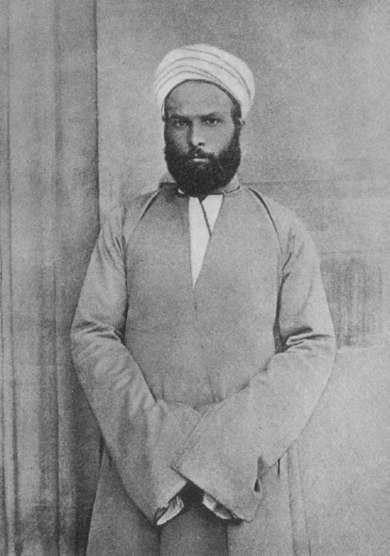
\includegraphics[width=.7\textwidth]{CourantsIslamContemporain/ImagesCourantsIslamContemporain/390px-Muhammad_Abduh.jpg}
       \caption{\href{https://fr.wikipedia.org/wiki/Mohamed\_Abduh}{Muhammad Abduh}}
       \label{fig:my_label}
   \end{marginfigure}
   Surtout en Egypte mais a partagé le séjour parisien de \textit{Aghani} puis au Liban. On lui a interdit d'enseigner mais il a été nommé grand mufti d'Egypte (1899). On avait moins peur de son activité du droit que de son activité sur les jeunes en tant qu'enseignant. Fonde aussi une école qui va évoluer différemment.  
    
    \paragraph{Avancée coloniale plus avancée} La colonisation s'est accentuée : les occidentaux apparaissent comme une menace politique. Peur du colonialisme. Le positivisme s'est aussi accentué. Ils doivent se situer dans le rapport entre Foi et Raison. 
   
   \paragraph{Héritiers du pre-réformisme} En inde en particulier, décadence du monde musulman. beaucoup plus faibles que l'occident, parce que \textit{nous avons perdu l'authenticité de la Foi musulmane}. Pour retrouver notre puissance, il faut retrouver l'authenticité de la pratique et la Foi musulmane.
   
   \paragraph{Mais des différences} Mais la différence avec la pré-reforme, cela passe par la pensée des lumières qu'ils accueillent de façon positive. Importance de la \textit{raison}. Par ailleurs, à la suite de \textit{Guizot}\sn{François Guizot, \textit{Histoire de la Civilisation en Europe}}, il pense l'Islam comme civilisation et pas uniquement comme Religion. Qui dit civilisation implique Progrès. 
   
  
  %----------------------------------------------------------------------------------- 
  \section{Foi et raison}
  
 \paragraph{Renan } Dans un discours retentissant à la Sorbonne, il affirme que les races sémites sont opposées à la Raison.
 
 \paragraph{Réponse d'Afghani} La critique de la religion par le positivisme est fondé, surtout pour le christianisme : Trinité, incarnation, \ldots Et ce qui explique son succès en Occident. En revanche, ce n'est pas vrai en Islam.
 
 \paragraph{Seyyed Ahmad Khan} \label{Theol:AhmadKhan} parfaite adéquation entre la vérité naturelle et révélée. 
 \begin{quote}
    \textit{ Islam is nature and Nature is Islam}
 \end{quote}
 Il ne regarde que le Coran et lecture du Coran à l'aune des vérités naturelles. Lecture allégorique quand le Coran n'est pas cohérent avec la nature. La Loi doit découler de la Loi Naturelle, de la Raison. 
 
 \paragraph{Al Afghani} Un peu en retrait. Il y a adéquation entre la loi naturelle et révélee. Discours \textit{concordiste} \sn{Vision concordiste : très présent aujourd'hui : on trouve en germe toutes les réalités scientifiques (ex : on trouve la vitesse de la lumière, foetus, \ldots). Visée apologétique. Explication rationnelle scientifique des actes musulmans (le jeune du ramadan est bon pour la santé)} mais il dit : 
 \begin{quote}
     Malgré cela, on ne peut pas se passer de la révélation; la Raison de l'homme est entravée par ses Passions . 
 \end{quote}
  La révélation et en particulier le jugement, permet un jugement éthique et moral. 
  
  \paragraph{Muhammad Abduh } Distinguer Raison et révélation, qui se complètent. La Raison peut atteindre les dogmes fondamentaux :  permettre de savoir que Dieu existe, \ldots
  Mais elle ne nous permet pas de révéler le culte ni la raison pratique : ou est le bien, où est le mal ? La vie morale est basée sur la Révélation mais la Raison doit être utilisée pour interpréter la Révélation dans les cas concrèt.
  
  %-----------------------------------------------------------------------------------
  \section{Retour aux sources et \emph{ijtihad}}
  
\paragraph{Ijtihad} Surtout Ahmad Khan et Abduh vont travailler la Sunna avec un regard critique. 
 On retrouve aussi le taqlid (neg) vs ijtihad.
 
\begin{Def}[taqlid]
  \emph{ imitation (servile)}
\end{Def} 
Pour Abduh, le taqlid est lié aux turcs pour soumettre les populations (vision nationaliste arabe), et aussi le soufisme qui a encouragé le taqlid. Les écoles de Abduh sont assez négatives sur le soufisme. \mn{Sahah Hassein ? raconte dans ses mémoires comment dans une école de Abduh, le soufisme était vu de façon négative }. 

\paragraph{Revenir aux sources} Revenir aux temps du Prophète pour reprendre le \textit{principe dynamique} qui était à l'origine, avec une vision positive de la Raison. Il ne s'agit pas d'imiter le Prophète mais de retrouver la dynamique. 

\paragraph{Relecture} des textes du Coran pour repenser le droit (Abdh est jurisconsulte) et en reclassifiant les hadiths. Il revalorise l'opinion personnelle du jurisconsulte (\emph{ra'y}) contre le conservatisme de \emph{l'ijma}. 


\begin{Def}[ijma]

\emph{` consensus des ulamas}
\end{Def} 

\begin{Synthesis}
Il faut chercher l'intention du droit pour rentrer dans un dynamisme juridique
\end{Synthesis}



  %-----------------------------------------------------------------------------------
  \section{L'action: politique et éducation} 
 
Dans le pré-réformisme, on avait vu l'importance de l'action sociale. On a la même perspective ici : il faut agir et transformer la société.

\paragraph{Afghani} est d'abord un homme d'action et politique. Pour retrouver sa grandeur, il faut commencer par émanciper le monde musulman. \textit{Le politique prime}, vision panislamique unifiée (pas forcément un seul état, mais des états coordonnés), émancipée du monde occidental. Risque d'instrumentalisation de l'Islam pour une fin politique.

\paragraph{Renouveau d'abord} avec Kan et Abduh : le peuple n'est pas mur pour être indépendant. Et donc plus conciliants vis à vis des colonisateurs. Avec un discours nationaliste plus que pan-islamique. La priorité était donc \textit{l'éducation}. C'est la raison de la rupture entre Abduh et Afghani. 
\begin{itemize}
    \item Collège d'Aligarh\sn{\href{https://en.wikipedia.org/wiki/Aligarh_Muslim_University}{Université musulmane}} : éducation islamique et ensuite occidentale. En Inde. Une des grandes réalisations d'Ahmad Khan. Creuset de formation de tous les réformistes indiens.
    \item volonté de reforme d'Al Azhar. Il n'a pas réussi mais ses disciples ont réussi à modifier par touches la formation (en revenant aux théologiens à la source)
\end{itemize}

\paragraph{Souveraineté populaire} Il faut éduquer les gens à leurs droits et leurs devoirs pour pouvoir fonder une démocratie. Ils ont une volonté de développer des écoles gratuites mais impact limité. Leur désir de s'engager sur le terrain est un semi-échec.


  %-----------------------------------------------------------------------------------
\hypertarget{glossaire-2}{%
\subsection{\texorpdfstring{{Glossaire}}{Glossaire}}\label{glossaire-2}}


\paragraph{Personnes}

Ibn Taymiyya

Jamal ad-din Al-Afghani (1839-1897) Khayr-ad din Pacha (1820- 1889)

Muhammad `Abduh (1849-1905) Seyyed Ahmad Khan (1817-1898) (prononcer ARMA CRAN)  Shah Walli
Allah

Tahtawi (1801-1873)

\paragraph{Lieux}

Al-Azhar Aligarh

\paragraph{Autres noms propres}

naqshbandi

al-`Urwa

al-Wuthqa

mu`tazilite

nayshariyya

\paragraph{Notions}

\begin{Def}[bid\emph{`}a ]
\emph{: innovation}
\end{Def} 

\begin{Def}[\emph{`}ibadat]

 \emph{ culte ( et partie du droit traitant du culte)}
\end{Def} 
 

\begin{Def}[maslaha]
 \emph{intérêt général, bien commun}
\end{Def} 

\begin{Def}[mu\emph{`}amalat]
  \emph{ relation (et partie du droit traitant des
relations humaines)} 
\end{Def} 



\begin{Def}[qasd]
 \emph{ principe de consultation}
\end{Def} 

\begin{Def}[talfiq]
  \emph{interprétation
éclectique}
\end{Def} 




\hypertarget{muhammad-abduh-1849-1905}{%
\subsection{\texorpdfstring{{Muhammad `Abduh}
(1849-1905)}{Muhammad `Abduh (1849-1905)}}\label{muhammad-abduh-1849-1905}}

Discours évolutioniste.

\begin{quote}
  Quand les religions firent leur apparition, les êtres humains ne
comprenaient leur intérêt, général ou particulier, que de la façon la
plus rudimentaire, plutôt comme des enfants nouveau-nés qui ne
connaissent que ce qui leur tombe sous les sens et ne distinguent
qu'avec difficulté entre le présent et le passé. Ils ne reconnaissent
vraiment que ce qu'ils touchent manuellement et leur état de conscience
ne leur permet pas de "sympathiser" avec leur famille ou leurs
compagnons, tant ils sont obnubilés par leur survie pour pouvoir
s'intéresser aux implications de leur relation aux autres, à moins qu'il
ne s'agisse d'une main qui les nourrit ou les remet sur leur pieds. Dans
ce contexte, les religions ne pouvaient s'adresser intelligemment aux
hommes en abordant les subtiles dimensions de la conscience ou en leur
faisant étalage de preuves rationnelles. Au contraire, la grande grâce
de Dieu se voit dans la manière dont ces religions s'adressèrent aux
peuples comme à des enfants, à la façon de parents qui éduquent leur
enfant avec la plus grande simplicité en se servant des sens de l'ouïe
et de la vue. Les religions prirent les hommes et leur donnèrent des
commandements directs ainsi que des prohibitions fermes exigeant la plus
complète obéissance. Bien que le sens et le but en pouvait être connu,
l'obéissance ne dépendait pas du degré de compréhension ni de
l'exactitude du savoir. Les religions fournirent aussi des miracles
étonnants et impressionnants et imposèrent des formes de culte adaptées
à la condition des hommes.
    
\end{quote}
Les religions (ici surtout le judaisme) sont visées.

\begin{quote}
Au cours des siècles suivants, les peuples connurent grandeur et déclin,
progrès et régression. Ils se querellèrent et se réconcilièrent. Les
siècles apportèrent leur cortège de souffrances et une alternance
ininterrompue de prospérité et d'adversité qui suscitèrent une
sensibilité plus affinée, une conscience plus aiguë que l'on peut
utilement comparer à ce qui se passe dans les cœurs féminins ou à l'âge
de l'adolescence. Une religion survint alors qui parlait à ces
sentiments et, s'adressant tendrement à ces compassions, fit appel aux
doux émois du cœur. Elle donna aux humains les lois sacrées de
l'ascétisme, les éloignant complètement du monde et les tournant vers
une vie plus haute. Elle enseigna aux hommes à ne pas défendre leurs
droits si évidents qu'ils soient et ferma la porte du ciel aux riches.
D'autres traits du même genre caractéristiques de cette religion nous
sont bien connus. Elle établit des formes de culte divin qui
s'harmonisaient avec sa compréhension de l'être humain et le sens de son
message. Elle fut remarquablement efficace pour corriger les défauts et
chasser le mal des âmes qui lui étaient soumises. Mais seulement
quelques générations plus tard, les hommes se lassèrent, s'affaiblirent
et se détournèrent. Ils abandonnèrent ses exigences et ses préceptes les
trouvant au-dessus de leurs forces. Ils se mirent à penser que ces
commandements étaient naturellement impraticables. Même les cadres de
cette religion se mirent à faire concurrence aux rois dans leur autorité
et aux riches oisifs dans leur richesse. La grande masse du peuple
perdit sa noblesse au moyen de "l'interprétation"\sn{sens négatif. Peut être référence à la falsification des écritures, critique des musulmans au christianisme} et, emporté par de
folles passions, introduisit toute sorte d'innovations.
\end{quote}

Dans une logique évolutionniste, le christianisme est un développement.


\begin{quote}
Ainsi se passèrent les choses, tant dans l'activité que dans les
attitudes profondes. La pureté était oubliée et l'intégrité mise aux
enchères. Quant aux dogmes, ils furent infectés par le schisme et
l'hérésie. Les gardiens de la foi en abandonnèrent tous les principes à
l'exception d'un seul qu'ils croyaient - à tort - être le pilier
principal de leur foi et son fondement principal, à savoir
l'interdiction de l'examen rationnel de la foi et même des complexités
de l'univers ou de l'exploration des replis secrets de l'intelligence.
Ils promulguèrent le principe que la Raison et la Religion n'avaient
rien de commun, mais plutôt que la religion était l'ennemi juré de la
Science. Ce principe n'était pas laissé simplement au choix de chacun:
au contraire, ils l'imposèrent énergiquement comme la chose à faire par
tous et chacun. Ils imposèrent la doctrine avec une telle énergie qu'ils
déclenchèrent le plus honteux de tous les conflits de l'Histoire de
l'humanité, à savoir la guerre civile dans la maison de la religion pour
imposer des consignes religieuses\sn{Guerre de Religions}. Ainsi furent détruits les fondements
eux-mêmes et brisées les liens internes à la communauté. La concorde, la
coopération et la paix disparurent: le schisme, la dispute et la
querelle régnèrent à leur place. Ainsi survécut l'humanité jusqu'à
l'avènement de l'islam.
\end{quote}
Dans le Coran, le fait que les chrétiens soient divisés est une preuve que le message est falsifié.

\begin{quote}
Enfin la société humaine atteignit le point où l'homme parvient à sa
pleine stature, à l'aide d'une réflexion morale sur les vicissitudes
passées. L'Islam survint pour présenter son message à la Raison, pour
appeler à l'action l'esprit et l'intelligence, pour prendre l'émotion et
les sentiments comme partenaires afin de guider l'homme vers le bonheur
terrestre aussi bien que céleste. Il mit en lumière les causes des
discordes humaines et démontra que, devant Dieu, la religion était
unique à travers toutes les générations, qu'il n'y avait qu'un seul
projet divin visant à les réformer et à les purifier intérieurement.
L'Islam enseigna que le seul but des formes extérieures de culte était
de renouveler le recueillement intérieur nous centrant sur Dieu et que
Dieu ne regarde pas les apparences mais le cœur. Il demanda au croyant
de s'occuper du corps aussi bien que de l'âme, exigeant l'intégrité
extérieure aussi bien que l'intérieure qu'il rendit également
obligatoires. La sincérité devint le centre du culte et les rites ne
furent imposés que dans la mesure où ils conduisaient à la
sanctification de la personnalité morale.
\begin{quote}
    "En vérité, la prière préserve
les hommes du mal et des souillures". (Cor. 29,45) "L'Homme a été créé
instable {[}très inquiet{]}; quand le malheur le touche, il est abattu;
et quand le bonheur le touche, il est refuseur. Sauf ceux qui pratiquent
la Salat". (Cor 70,19-22) 
\end{quote} 
L'homme riche qui se souvient d'être
reconnaissant est élevé par l'Islam au même niveau que le pauvre qui
souffre patiemment. Peut-être même l'Islam lui porte-t-il une plus haute
estime encore. L'Islam, dans ses exhortations, s'adresse à l'homme comme
un sage et sobre conseiller s'adresserait à une personne mûre pour
l'appeler à mettre en œuvre toutes ses facultés, externes ou internes.
Il proclame sans équivoque que c'est là le moyen de plaire à Dieu et de
Lui montrer notre reconnaissance pour sa Grâce. Ce monde reçoit la
semence du monde à venir. Les hommes ne parviendront à leur fin ultime
qu'en se mettant à bien agir dans le présent.
\end{quote}


\begin{quote}

L'Islam délivra la raison de toutes ses chaînes, il la libéra de
l'imitation aveugle qui l'avait asservie, il lui rendit son domaine dans
lequel elle tranche selon son jugement et sa sagesse ; toutefois elle
doit s'incliner devant Dieu seul et s'arrêter aux limites posées par la
religion; mais au-dedans de ces limites , il n'y a pas de barrière à son
activité et il n'y a pas de fin aux spéculations qui se déroulent sous
ses auspices.

Tiré de M. `Abduh, \emph{Risalat at-Tawhid} (\emph{Traité de l'Unité
divine}, Paris, 1925)
\end{quote}
\begin{Synthesis}
L'Islam est la religion de la maturité, marqué par la raison. Mais l'Islam tient l'équilibre. 
\end{Synthesis}

Equilibre entre : 
\begin{itemize}
    \item entre la Religion de la Raison mais on intègre les sentiments. Le culte extérieur sert le culte intérieur. 
    \item pour les riches et les pauvres
    \item avec la Loi et Raison
\end{itemize}

\begin{Synthesis}[Mouvement moderniste]
Au XIX, le mouvement réformiste intègre la Raison et le Progrès comme des acquis des Lumières. Ces lumières ne sont pas incompatibles avec l'Islam, religion de la raison et les lumières occidentales venant de la Renaissance et de la pensée grecque via la \textit{falsafa}.
Le réformisme est complexe mais ce n'est pas la seule religion pour laquelle c'est compliqué : tension entre le retour aux sources et l'acceptation de la modernité.
'Abdub a été en equilibre et ses disciples vont accentuer le retour aux sources ou au contraire l'accueil de la modernité. 
\end{Synthesis}


\chapter{{Tendances sécularistes et nationalistes}}
  \mn{(14/02/2022)}
 
 \subsection{Bibliographie}
 
  ABDERRAZIQ, Ali \emph{L'Islam et les fondements du pouvoir}, La
  Découverte/ Cedej, Paris, 1994.
 
*BOZARSLAN, Hamit \emph{Histoire de la Turquie contemporaine}, La
Découverte, Repères, 2004. DEVLIN, John F \emph{The Ba`th Party}, Hoover
Institution Press, Stanford, 1979.

FILALI-ANSARY, Abdou \emph{L'islam est-il hostile à la laïcité ?},
Arles, Actes Sud, 2002. HOURANI, Albert \emph{La pensée arabe et
l'Occident,} Groupe Naufal Europe, Paris, 1991.

PISAI « Courants actuels dans l'Islam: le Ba`t », \emph{Etudes Arabes},
n° 63 \& n° 64, 1982-3.
 




\section{Introduction}
\begin{Def}[Sécularisme]
Une évolution juridique et politique vers un modèle Européen, et un affaiblissement des structures religieuses dans l'Etat et la société
\end{Def}

Ce courant va globalement s'imposer jusqu'aux années 1960/70 avec trois courants : 
\begin{itemize}
    \item Elites politiques qui ont grandi dans des écoles occidentales, missionnaires ou réformistes. Ces élites (Ataturk,..) faisant des études en Europe. Ils vont recommander une\textbf{ sécularisation à l'occidentale} (Bourghiba,...). Les deux pays qui n'ont pas été colonisés (Turquie, Iran) ont été les pays qui ont connu la sécularisation à l'occidentale la plus ferme.
    \item les disciples de 'Abduh qui cherchent à penser la \textbf{sécularisation dans le cadre islamique}
    \item rencontre du premier courant avec la \textbf{pensée socialiste} : nationalisme arabe
\end{itemize}
 ~
   %----------------------------------------------------------------
  \section{Le sécularisme d'importation
  occidentale : le modèle
  turc}

  

  
    
    \subsection{Aux racines : les Jeunes Turcs}
Ils vont être moteurs de la révolution constitutionnelle de 1908\sn{La révolution des Jeunes-Turcs de l'Empire ottoman en juillet 1908 est un soulèvement au cours duquel le mouvement des Jeunes-Turcs restaure la Constitution de l'Empire ottoman de 1876 et inaugure la politique multipartite dans un système électoral à deux étapes sous le parlement ottoman.}. 
Les tribunaux religieux sont placés sous la responsabilité du ministère de la Justice (entre 1908 et 18). 
    
      \subsection{La République de Mustapha Kemal}
\paragraph{Mustapha Kemal ou \textit{Atatürk}} Officier charismatique. il s'empare du pouvoir en 1923. Il crée une république à l'image de la France et en devient le chef. Politique très séculariste. 
\begin{itemize}
    \item Rejet du passé Ottoman après la défaite de 1918, qui se serait affaibli via les influences arabes et persanes, et la place que l'Islam y a joué.
    \item  Permet d'éviter les contre-pouvoirs en particulier confrériques. 
\end{itemize}

\paragraph{Soumettre l'Islam au contrôle de l'Etat}
\begin{itemize}
    \item 1924 : Abolution du Califat et expulsion. On crée une présidence des affaires religieuses qui nomme les imams, administre les mosquée, supervise les \textit{muftis}. Les imams sont des fonctionnaires. Le \textit{Diltib}.
    \item unification de l'enseignement (on ferme toutes les institutions religieuses supérieures : medrese) et on crée des Ecoles d'enseignement supérieur pour Imam d'Etat.
    \item 1925 : confréries religieuses sont interdites
    \item 1926 : code civile suisse introduit
    \item 1928 : l'Islam n'est plus religion d'Etat
    \item 1937 : le principe de laicité dans la constitution.
\end{itemize}

Des mesures symboliques : 
\begin{itemize}
    \item 1925 : interdiction du Fez
    \item 1926 : calendrier grégorien, avec dimanche comme jour férié (1935)
    \item 1928 : alphabet latin. 
    \item 1928 : Sainte Sophie devient Musée
\end{itemize}


\paragraph{moderniser l'Islam}

Rapport en 1926 : "perspective scientifique". Vision positiviste
\begin{itemize}
    \item Des mosquées propres avec des bancs
    \item instruments et musiques sacrées (on veut imposer le modèle chrétien)
    \item former les imams à la philosophie et aux sciences occidentales
\end{itemize}

\paragraph{intégrer l'Islam dans l'idéologie Turque}
Cela passe par un islam turc; remplacer l'arabe par le turc. On arrête l'apprentissage l'arabe et le perse. On traduit donc le Coran et la Sunna en Turc (mais il n'est pas utilisé finalement dans le culte). 
En 1932, l'appel à la prière en turc (mais refus de la population et il fait marche arrière).

\paragraph{L'utilisation de l'Islam comme une composante du nationalisme turque} Entre 1923 et 1930, vaste échange avec la Grèce, le critère n'a pas été un critère linguistique mais un critère religieux (chrétien turcophone). 
En tant que population musulmane sunnite, les kurdes ne peuvent être une minorité, seules les populations chrétiennes, juives,... peuvent être considérées comme une minorité. Les alévites ne sont pas reconnus comme une minorité (musulmans = sunnites). De même, la religion est mentionnée sur la carte d'identité. 
\begin{Synthesis}
\textit{une intégration de la religion dans l'Etat} et non une séparation. 
  
\end{Synthesis}

\paragraph{Ziya Gökalp
(1876-1924)}    Un jeune turc penseur de la Turquie d'Ataturk.
  \begin{quote}
Maintenant\mn{Ziya Gökalp Extraits traduits d'un ouvrage hostile au modernisme musulman:

Maryam Jameelah, \textit{Islam and modernism}

(Md Yusuf Khan, Lahore, 1968), 
p. 101-107} la mission des Turcs ne doit être que celle de découvrir le
passé pré islamique Turc qui est resté ancré dans le peuple et y greffer
la civilisation Occidentale dans sa totalité. Pour égaler les pouvoirs
européens militairement et dans les sciences et l'industrie, notre seule
voie de salut est d'adopter la civilisation Occidentale complètement! \sn{(Ziya Gökalp, \textbf{Turkish Nationalism and Western Civilisation},
New-York, 1959, p. 276.)
}

Parmi les Turcs pré-islamiques, le patriotisme a atteint ses niveaux les
plus hauts. Dans l'avenir, comme dans le passé, le patriotisme doit être
le point de moralité le plus important pour les Turcs parce que la
nation et son âme sont en fin de compte la seule unité qui existe de
soi. La fidélité à la nation doit avoir la priorité sur la fidélité à la
famille ou la religion. Le Turkisme doit donner la priorité la plus
haute à la Nation et à la Patrie. Nous créerons une civilisation
véritable - une civilisation Turque qui suivra la croissance d'une
Nouvelle Vie. Classifier les Turcs, qui sont plus justes et plus beaux
que les Aryens, avec la race Mongole n'a aucune base scientifique. La
race Turque n'a pas dégénéré - comme d'autres races, par l'alcool et le
dérèglement des moeurs. Le sang turc est resté jeune et s'est durci
comme l'acier avec la splendeur du champ de bataille. L'intelligence
turque n'est pas usée; ses sentiments ne sont pas affaiblis. On promet
la conquête de l'avenir à la résolution Turque. (Ibid., pp. 302, 271 et
60.)

La civilisation occidentale est une suite de la civilisation de la
Méditerranée antique. Les fondateurs de la civilisation de la
Méditerranée étaient des peuples Turcs comme les Sumeriens, Scythes, le
Phoeniciens et les Hyksos. Il y a eu un Âge Touranien dans l'histoire
avant les âges antiques car les habitants les plus anciens de l'Asie
Occidentale étaient nos ancêtres. Ainsi nous faisons partie de la
civilisation Occidentale et avons part intégrale à cette civilisation.
(Ibid-, pp. 266- 7)

Quand une nation parvient aux étapes les plus hautes de son évolution,
elle trouve nécessaire de changer aussi sa civilisation. Quand les Turcs
étaient des membres d'une tribu nomade en Asie Centrale, ils ont
appartenu à la civilisation de l'Extrême-Orient. Quand ils ont passé à
l'étape de l'état Sultanesque, ils sont entrés dans le secteur de
civilisation Byzantine. Et aujourd'hui dans leur transition à l'état de
nation en tant qu'Etat séculier, ils sont déterminés à accepter la
civilisation Occidentale. (Ibid., pp. 270-1)

La grande erreur des autorités du Tanzimat\sn{Le mouvement des Tanzimat fut le premier essai de
réforme et de modernisation de l'empire Ottoman vers le milieu du
19\textsuperscript{ème} siècle.} était leur
tentative de créer un amalgame mental composé d'un mélange d'Orient et
d'Occident. Ils n'ont pas réalisé que les deux, avec leurs principes
diamétralement opposés, ne pouvaient pas être réconciliés. La dichotomie
présente dans notre structure politique, le système double de tribunaux,
les deux types d'écoles, les deux systèmes de taxation, deux budgets,
les deux jeux de lois, sont tous les produits de cette erreur ... Toute
tentative de réconcilier Orient et Occident conduit à perpétuer des
conditions médiévales dans l'âge moderne et à essayer de les maintenir
en vie. De même qu'il était impossible de réconcilier des méthodes
janissaires avec un système militaire moderne, de même qu'il était
futile de synchroniser la médecine dépassée avec la médecine moderne,
ainsi est-il inutile de continuer, côte à côte, les vieilles conceptions
de la loi et les nouvelles ; les standards moderne d'éthique et les
traditionnels. Chaque civilisation a sa propre logique, ses propres
standards esthétiques, sa propre perspective du monde. Pour cette
raison, des civilisations différentes ne peuvent pas se mélanger
librement l'une avec l'autre. De nouveau, pour la même raison, quand une
société ne prend pas pour système une certaine civilisation dans sa
totalité, il ne réussit pas davantage à en prendre ses composantes. Même
s'il en prend quelques parties, il ne réussit pas à les digérer et à les
assimiler. Nos réformateurs des Tanzimat, qui ont échoué comprendre ce
point, prenaient toujours des demi-mesures dans ce qu'ils ont essayé de
faire. Avant qu'ils n'aient pris de mesures pour moderniser la
production nationale, ils ont voulu changer les habitudes de
consommation, les vêtements, l'alimentation, le bâtiment et les meubles.
D'autre part, on n'a même pas construit un noyau d'industrie digne des
standards européens parce que
les décideurs de la politique des Tanzimat ont essayé leurs réformes
sans en étudier les conditions et sans fixer des buts et des plans
précis. (Ibid., pp. 270-7).

Le but du Turkisme dans la loi est d'établir un système de loi moderne
en Turquie. La condition la plus fondamentale de notre succès à
rejoindre les rangs des nations modernes consiste à effectuer un
nettoyage complet de toutes les branches de notre structure légale pour
y effacer toute trace de théocratie et de cléricalisme. L'état qui est
libre de ces deux caractéristiques de l'état médiéval est appelé un état
moderne. En premier lieu, dans un état moderne, le droit de légiférer et
d'administrer directement appartient au peuple. Aucune fonction, aucune
tradition et aucun autre droit ne peuvent restreindre et limiter ce
droit. En second lieu, tous les membres de la nation moderne,
indépendamment de leur affiliation religieuse, sont considérés comme
égaux en tous points. Bref, toutes les dispositions existant dans nos
lois qui sont contraires à la liberté, à l'égalité et à la justice ainsi
que toutes les traces de théocratie et de cléricalisme doivent être
complètement éliminées. Le Turkisme est un mouvement séculier et ne peut
accepter que des mouvements de nature séculière. (Ibid., pp. 304-5).

C'est seulement au moyen de sa civilisation que l'Europe a été capable
de défaire les nations Musulmanes et est devenue le Maître du monde.
Pourquoi, alors, devons-nous hésiter à adopter cette même civilisation
qui s'est prouvée si capable de réussir ? Notre foi Musulmane ne nous
fait-elle pas un devoir de rechercher toutes les sortes de science et de
savoir comme notre Saint Prophète lui-même nous l'a dit, "Cherchez la
connaissance même si c'est en Chine," et "l'Étude est la propriété
perdue du croyant ; il doit la prendre partout où il la
trouve"?\sn{ Citations de deux hadiths souvent repris par les
apologètes de l'Islam pour montrer la compatibilité de la foi musulmane
avec la science. L'auteur les exploite d'une façon différente pour
inciter les lecteurs musulmans à s'ouvrir aux valeurs occidentales.} Le Japon est considéré comme puissance européenne
mais nous sommes toujours considérés comme une nation Asiatique à cause
de notre retard à accepter véritablement la civilisation européenne.
(Ibid., pp. 266-7).

La terre où l'appel à la prière résonne en Turc et où ceux qui prient
comprennent la signification de leur religion ; la terre où le Coran est
appris en Turc et où chaque homme, grand ou petit, connaît parfaitement
le commandement de Dieu - Ô fils de la Turquie, cette terre est ta
Patrie!


    
\end{quote}
    
    
    \begin{Synthesis}[Ziya Gökalp]
      Il s'appuie sur une analyse raciale typique du XIX, en valorisant la race turque qui est à l'origine de la civilisation occidentale  (Phénicien, Hyksos,...) par rapport à l'abâtardissement arabe ou perse.
      Puis en proposant une vision comparable à l'ère Meiji du Japon, se calant sur l'Occident, sans essayer un mélange, ce qui explique les mesures symboliques pour rompre avec le passé, ainsi que la sécularisation.
      Légitime par l'Islam les choix qu'il pose.
    \end{Synthesis}
    Ils n'ont pas vraiment pensé le culte musulman (cf la proposition des bancs). Pas une véritable articulation entre valeur occidentale et Islam mais en utilisant l'Islam comme un slogan.
    

    
  


 ~
   %----------------------------------------------------------------
  \hypertarget{les-disciples-de-abduh}{%
  \section{\texorpdfstring{{Les disciples de
  Abduh}}{Les disciples de Abduh}}\label{les-disciples-de-abduh}}

  

  
    
      \subsection{Qasim Amin et le statut des femmes (1863-1908)}
    
    \paragraph{Qasim Amin} voyage en France en 1880. Il a été dans le cercle de \textit{Afghani} à Paris. Revient au Caire - Modernisation de l'universation.
    
    \paragraph{1899 - La libération des femmes} Un livre qui va faire un grand remous. Un diagnostic du déclin de la civilisation musulmane, liée à l'affaiblissement des vertus morales et sociales. Il faut donc renforcer l'éducation à la maison qui se fait par les femmes, dont il faut relever le statut. Education féminine jusqu'au primaire pour éduquer les enfants et travailler (seule façon de garantir ses droits dans le foyer). 
    
    \paragraph{voile} Il pose aussi la question du voile intégrale \mn{lire Naguib Mahfouz, \textit{Impasse des deux palais} qui raconte une femme bourgeoise recluse}, qui empêche la femme bourgeoise de travailler et d'avoir un rôle dans l'Espace public.
    
    \paragraph{Interdiction de la polygamie} 'Abduh s'était positionné contre. Plus que 'Abduh, il s'oppose à la répudiation trop facile et prône une égalité de traitement homme / femme. Il a des arguments religieux pour cela.  Le Coran autorise plusieurs femmes à partir du moment où on est parfaitement équitable, ce qui est impossible. 
    
    \paragraph{Une réaction importante} beaucoup d'oppositions et le livre n'aura pas d'impacts à court terme. A noter néanmoins la figure de \textit{Hoda Sha'rawi} première feministe arabe, Egyptienne : Egypte, centre du féminisme arabe.
  
    
      \subsection{Ali Abderraziq et la laïcité (1888-1966)}
    
    \paragraph{Ali Abderraziq} Egyptien, famille liée à 'Abduh, séjour en Angleterre. Carrière de juriste. 
    
    \paragraph{Abolition du Califat en 1926} Il faut nommer un nouveau Calife, le Sherif de la Mecque par exemple. Un congrès au Caire pour réfléchir au Califat.
    \begin{itemize}
        \item Le Califat est légitime et nécessaire
        \item mais actuellement non réalisable du fait de l'impossibilité d'un pouvoir temporel
    \end{itemize}
  
  \paragraph{1925 : L'islam et les fondements du pouvoir } Le Califat n'a aucune légitimité en Islam. Dans le Coran et la Sunna, pas de réalité politique du Califat. Institution humaine imposée par les armes par les successeurs. Mohammed avait un pouvoir de type charismatique, prophétique. Les hommes reconnaissaient son pouvoir par son charisme. Mais pas de volonté de Dieu de fonder un pouvoir politique. Sinon, Dieu aurait indiqué à Mohammed de nommer un successeur. Les successeurs de Mohammed ont imposé un pouvoir royal en imposant un pouvoir politique et religieux.  Fait historique qui a nuit à l'Islam (collusion entre pouvoir politique et savant, Islam de passivité), cela a empêché le développement d'une pensée politique en Islam. 
  
  \paragraph{La shari'a comme prescriptions éthiques} ne fonde pas un système légal.
  
  \paragraph{Dieu ne se soucie pas de la forme politique du Gouvernement}  Les hommes doivent utiliser leur raison pour définir la forme de gouvernement. 

  \paragraph{unité de l'umma ni possible ni souhaitable} un verset "différentes familles... pour les bonnes oeuvres".

\paragraph{Une remise en cause forte de l'Islam} Remet en cause le statut prophétique de Mohammed et les débuts de l'Islam avec un âge d'or (\textit{les califes bien guidés}). Des fatwas de Al-Azhar qui l'interdisent d'enseigner.  Aujourd'hui, des penseurs religieux le relisent en essayant de penser l'interaction entre Islam et les formes de gouvernance. \sn{lire par exemple le livre de Filali-Ansary, \textit{l'islam est il hostile à la laïcité ?}, Marocain. Voir aussi le texte D\textit{iffusion de la pensée réformiste en Egypte : un témoignage}}
 ~
   %----------------------------------------------------------------
  \hypertarget{islam-nationalisme-et-ruxe9volution}{%
  \section{\texorpdfstring{{Islam, nationalisme et
  révolution}}{Islam, nationalisme et révolution}}\label{islam-nationalisme-et-ruxe9volution}}


  
    
      \subsection{Le nationalisme arabe}
    
  
  \paragraph{discours nationaliste arabe 1920-1930} Dans les élites sécularisées, on va penser l'Islam moins comme une religion qu'une \textit{culture}. Ce qui a créé la nation Arabe, sa culture, l'objet de sa fierté collective. 
  
  \paragraph{Un mouvement qui nait au proche et moyen orient} car le référentiel est d'abord arabe, dans des pays avec une faible vision nationaliste.
  
  \paragraph{Agrégation des chrétiens et minorités arabes non islamique} Selon Al-Bazzaz, L'Islam correspond à la moralité naturelle des arabes nomades de cette époque. Et donc tous ceux qui parlent arabes peuvent s'approprier ce passé islamique. Même les chrétiens parce qu'ils parlent arabe, peuvent s'agréger à ce nationalisme arabe.
   
      \subsection{Islam et révolution : la naissance du parti ba`th}


  \paragraph{Figure de Nasser} avec la rencontre du socialisme
   

 \begin{Def}[ba'th] : \emph{résurrection}
\end{Def}
 
 


 
\paragraph{{Michel `Aflaq
(1910-1989)}} 

\begin{quote}
    \mn{{Michel `Aflaq (1910-1989)}Publié dans \textbf{Etudes Arabes}, N° 63, 1982-2, \emph{Courants
actuels du monde arabe, le Ba't}, p. 100-102.}




Le Ba't arabe est apparu, dans la vie récente des Arabes, au milieu de
l'immobilisme, des reniements, de la recherche de l'intérêt personnel et
en pleine désintégration, le Ba't arabe est apparu comme un mouvement de
foi profonde qui polarise les cœurs purs et sains, qui attire les
volontés fortes et sincères, qui regroupe autour de lui les individus
emplis de l'amour de la Nation arabe, ceux qui ont foi en sa grandeur,
ceux qui ne se laissent pas aveugler par ses imperfections d'aujourd'hui
au point de ne plus voir son essence et les potentialités de son avenir,
ceux chez qui les illusions et les difficultés du présent n'ont pas
réussi à étouffer la volonté de travailler à révéler cette essence et à
réveiller ces potentialités. La croissance du Ba't arabe est une preuve
éclatante de foi, et une affirmation des valeurs spirituelles où la
religion prend sa source.

Mais cette qualité même, cette foi qui caractérise le Ba't arabe, c'est
elle qui lui fait comme une loi de se heurter à tous les mouvements qui
nient la foi ou se voilent sous une foi superficielle et contrefaite.
L'avènement du Ba't, il y a dix ans, fut une déclaration de guerre
ouverte au communisme en tant que mouvement matérialiste, négatif et
porteur de haine, et au nationalisme purement verbal qui était de mode,
qui représente la sécheresse, la stérilité et l'incapacité à créer, qui,
voyant dans la situation présente corrompue la vérité négative, perd
ainsi tout pouvoir clé maîtriser cette réalité. De même, il fallait
absolument s'opposer à la religiosité, courante alors, dans laquelle ces
mêmes défauts
se manifestaient. Le Ba't arabe dès sa création a défié ces phénomènes
malsains et les a tous renvoyés à une seule cause, à savoir la perte de
confiance en soi. Ainsi le communisme n'est qu'éveil factice pour ceux
qui ont perdu tout contact avec l'esprit de leur nation, qui ont
désespéré de toute libération qui viendrait de cette nation elle-même et
se sont satisfaits d'une libération qui viendrait de l'extérieur,
factice et suspecte. Le nationalisme avait accepté le mal comme un état
normal, avait pris son parti de l'égoïsme, de la servitude et du
mensonge comme des valeurs stables de la société, parce que se rebeller
contre ces maux eût exigé de lui qu'il fît confiance en la capacité de
la nation à s'en libérer. La piété avait perdu tout lien avec l'esprit
et les élans qui furent dans le passé la source de la religion, et qui
en firent un mouvement de renaissance, de renouvellement et
d'édification. Elle régressa vers un état de léthargie, de conservatisme
et d'obscurantisme, état qui ouvrit la voie toute grande au pharisaïsme
et à l'exploitation.

Le Ba't arabe appela à une conception nouvelle de la vie nationale et de
la vie en général. La base de cette nouvelle conception est la foi dans
les valeurs spirituelles et humanistes, dans la valeur de l'esprit arabe
authentique. Elle se manifeste dans la rupture définitive d'avec les
maux de la réalité présente, dans la lutte contre ces maux sur une route
montante et difficile qui conduira la Nation arabe, lentement et
laborieusement, à retrouver son âme par le moyen de ce combat jusqu'au
sang contre sa situation présente. C'est pourquoi il n'y a plus place,
dans la conception du Ba't arabe, pour quelque sentiment religieux que
ce soit qui n'assumerait pas cette foi exemplaire. Le Ba't arabe, qui
est un mouvement spirituel et actif, ne peut se séparer de la religion
ni se heurter à elle, mais il rompt avec l'immobilisme, l'égoïsme et
l'hypocrisie.

Le Ba't arabe est un mouvement nationaliste qui se tourne vers tous les
Arabes quels que soient leur confession ou leur "rite", qui considère
comme sacrée la liberté de croyance, qui regarde les religions comme
également sacrées et respectables. Mais, à côté de cela, il voit dans
l'islam un aspect national qui joua un rôle important dans la formation
de l'histoire arabe et du nationalisme arabe. Et le Ba't estime que ce
côté national de l'islam est en relation étroite avec l'héritage
spirituel des Arabes et les caractères propres de leur génie. Le Ba't
arabe fut le premier mouvement à mettre ce lien en évidence et à lui
donner sa forme définitive. Il a ouvert par là une crise qui dure encore
et il a sauvé le nationalisme arabe de deux déviations : celle du
nationalisme abstrait qui conduit fatalement à l'artificiel et à la
misère, et celle du nationalisme religieux qui le conduirait à la
contradiction et à la ruine.

Or l'islam, en tant que religion, est égal aux autres religions dans
l'Etat arabe qui traite tous ses citoyens sur un pied d'égalité et
respecte leur liberté de croyance. L'islam en tant que mouvement
spirituel qui a été intimement mêlé à l'histoire des Arabes, qui a été
imprégné de leur génie, qui a permis l'avènement de leur grande
renaissance, cet islam a une place particulière dans l'esprit du
nationalisme arabe, dans sa culture et dans le mouvement de son éveil.
Toutefois, ce rôle n'est absolument pas imposé, mais il naît de la
liberté, de la puissance de l'esprit, de ce que les Arabes sont
extrêmement attachés et en harmonie profonde et totalement libre avec
leur esprit. C'est en ce sens que le mouvement du Ba't arabe cherche
auprès de l'islam inspiration pour son renouvellement et pour sa révolte
contre les valeurs admises dans la société. Il puise à la source de
l'islam la foi, l'idéalisme et le renoncement à l'intérêt personnel et
aux séductions de ce siècle, dans le but de répandre les principes qui
libéreront les Arabes, aujourd'hui, de leur faiblesse, de leur désunion
et de leur bas niveau spirituel et social. Enfin, le Ba't arabe tire du
dynamisme éternel de l'islam\textit{ la force de résister au courant de la
réalité présente,} malsaine, il y trouve un exemple admirable à suivre
pour ce qui est du zèle sincère envers l'intérêt de la Nation, quand il
s'agit de soigner ses maux avec audace, franchise, sans chercher à
flatter à peu de frais les sentiments superficiels, et sans s'appuyer
sur les forces de l'obscurantisme, de la rancœur et de l'asservissement
de l'âme et de la pensée. Le Ba't croit fermement que cette méthode, qui
est en cohérence avec les principes sublimes qu'il proclame, c'est la
méthode à laquelle le succès est assuré, comme ce fut le cas dans le
passé et comme ce le sera toujours.


\end{quote}

\begin{Synthesis}
  Le mouvement Ba'th est un mouvement qui se veut spirituel (antimatérialiste), arabe mais pas islamique (même si la culture arabe en est imprégné).
  La dynamique spirituelle de l'Islam, c'est la \textit{Révolution}. Il faut combattre les institutions religieuses, les savants qui instrumentalisent la religion. 
\end{Synthesis}
 \begin{Def}[inqilâb]  : \emph{révolution}
\end{Def}
\paragraph{Syrie et Irak} Dans ces pays, le parti Ba'th s'est développé. Pas besoin de prôner l'Islam car en prônant la révolution, on trouve l'Islam authentique. D'où la sécularisation de ces pays. Le fait que Assad et Sadame Hussein appartiennent à des minorités religieuses a probablement joué.  
 ~
   %----------------------------------------------------------------
\hypertarget{glossaire-3}{%
\section{\texorpdfstring{{Glossaire}}{Glossaire}}\label{glossaire-3}}


{Personnes}

`Abd ar-Rahman al-Bazzaz Abdullah Cevdet (journal \emph{Içtihad}) Edmond
Rabbath

Kawakibi Michel Aflaq

Muhammad `Abduh Qustantin Zurayq Rashid Rida

Ziya Gökalp

{Lieux}

Al-Azhar

{Autres noms propres} naqshbandi

sheyh ül islam






 


\chapter{{Raidissement : de l'islam politique au salafisme}}
  \mn{(07/03/2022)}
 
 
 \section{bibliographie}
 
\begin{itemize}
\item

  HASSAN AL-BANNA \emph{Five tracts of Hassan al-Banna}, (1906-1949),
  Berkeley, University of California Press, 1978, (180 p.).

\item
  
  MAWDUDI \emph{Comprendre l'islam}, Paris, Association des étudiants
  islamiques en France, 1973.




ADRAOUI, Mohammed-Ali, \emph{Du Golfe aux banlieues : le salafisme
mondialisé}, Paris, PUF, 2013.

BENNOUNE Karima \emph{Votre fatwa ne s'applique pas ici}.
\emph{Histoires inédites de la lutte contre le fondamentalisme
musulman,} Paris, Temps présent, 2018.

NASR, SVR \emph{Mawdudi and the making of Islamic revivalism}, Oxford
university press, 1996.

FEILLARD, Andrée ; MADINIER, Rémy \emph{La fin de l'innocence. L'islam
indonésien face à la tentation radicale de 1967 à nos jours}, IRASEC-Les
Indes savantes, 2006.

GUIDERE, Matthieu \emph{Le printemps islamiste : démocratie et charia},
Paris, Ellipse, 2012. ROUGIER, Bernard (dir.) \emph{Qu'est-ce que le
salafisme ?}, Paris, PUF, 2008.

ROY, Olivier *\emph{Généalogie de l'islamisme}, Hachette, Paris, 1995.

SFEIR Antoine (dir.) \emph{Dictionnaire géopolitique de l'islamisme},
Paris, Bayard, 2009. TERNISIEN, Xavier \emph{Les Frères musulmans},
Fayard, Paris, 2005.
\end{itemize}



 
\section{{Au Proche-Orient arabe} :
  {émergence des Frères
  Musulmans}}

\subsection{Création : De Rashid Rida (1865-1935) à Hasan al-Banna (1906-1949)}

\subparagraph{Rashid Rida (1865-1935) } \label{Theol:Rida} Syrien. Formé de façon traditionnelle et aussi en parallèle occidental. \textbf{Mais ne fait pas le voyage en Europe} à la différence des générations précédentes\mn{On n'a plus besoin d'aller en Europe pour connaître l'occident}. Cela peut expliquer sa méfiance pour l'Europe. En 1997, rejoint le Caire pour se faire disciple d' 'Abduh. Publie \emph{El Manar}, un commentaire coranique, sensé être dans l'héritage de 'Abduh. Il a aussi oeuvré dans les Congrès pour la \textit{restauration des Califats}.

\subparagraph{Hasan al-Banna (1906-1949)} Égyptien. Vient dans une famille de notables ruraux, une famille gagnée par les idées réformistes. Études Coraniques puis études pour devenir Instituteur. Il rencontre une spiritualité soufie qui allie méditation et action \sn{Quelques influences des soufis : la structure des frères musulmans est proche des structures confrériques. Par ailleurs, les frères sont moins opposés au soufisme que d'autres mouvements radicaux}. De façon pragmatique, c'est là qu'il apprend la prédication et la Da'wa. En 1923, il va au Caire pour ses études : choc face au mode de vie occidental. Choc renforcé quand il arrive en 1927 à Isma'iliyya où les moeurs occidentaux sont très forts. 

\paragraph{Création des Frères musulmans et développement rapide} Banna crée en 1929 les \emph{les frères musulmans}, ils font la promesse pour donner leur vie pour ramener les Égyptiens à Dieu (\emph{Da'wa}). Les occidentaux corrompent les Égyptiens et détruisent le système social.15 sections en 1932; 1933 : section féminine et une section de jeunes. \textbf{1936 : un engagement politique, en Egypte et en Palestine}. il est arrêté en 1939 et on suspend ses publications. il est relaché en 1941, mais il continue son activité politique en Egypte et Palestine : 500 000 membres en 1945 et des sections dans les pays avoisinants (Palestine, Syrie, Soudan, Liban). 

\paragraph{Un mouvement clandestin} En 1948, les frères musulmans sont dissous. Banna est assassiné en 1949. Le mouvement continu de façon clandestine.

\begin{Synthesis}
Ils ne sont jamais allés en Occident. Ce ne sont plus des savants de la science coranique, des autodidactes. 
\end{Synthesis}

\paragraph{Défiance vis à vis de l'Occident} A la différence de la génération précédente, qui ne remettait pas en cause la supériorité de la société occidentale, il y a sur cette génération : un rejet du positivisme, de la notion du progrès, des dangers du matérialisme. Il y a même une conviction que l'Occident veut supprimer l'Islam comme système social. Les grands réformistes du XIX étaient sur l'Islam comme \textit{raison}. Alors qu'ici, on est sur une défense de type pragmatique, du cadre juridique traditionnel. Néanmoins, il n'y a pas de refus du progrès technique. \mn{En France, les frères musulmans ont eu une influence importante par les étudiants à partir de 1960. Tariq Ramadan, OEIF ne visent pas à transformer la société française en société islamique mais ont gardé le regard de défiance vis à vis de l'Occident et le regard très positif sur la société musulmane "l'Islamité" comme on parle de "chrétienté" }

\paragraph{ Un islam « radical »} Pour les réformistes, le rapport au source est un rapport \textit{dynamique}. Pour 'Abduh, les ancêtres (Salafs), les débuts de l'Islam va jusqu'au XI (et l'Imam ?), alors que l'on va avoir une tendance à réduire les ancêtres aux premiers califes, largement mythologisés. \textit{ordonner le bien et interdire le mal} Contrôle collectif, chaque musulman est responsable de veiller à ce que les autres musulmans suivent le bien. On raconte que Banna avait créé un commando en primaire pour faire respecter la loi musulmane par la force.

Pour les réformistes, l'Islam doit accompagner l'évolution de la législation, pour \textit{vivre mieux}. Alors que pour cette génération, il faut appliquer la sharia au sens strict.

\paragraph{Un islam actif et mobilisateur} Non seulement conscientiser le peuple via Une importance d'éduquer les masses, mais avec le but d'une orthopraxie islamique : 
\begin{itemize}
    \item Formations (journaux, cercles d'études\sn{ce n'est pas le modèle confrérie mais le modèle évangélique missionnaire}, maisons d'édition, )
    \item Educatif (création d'école : Banna crée une mosquée et une école à chaque section), lieu de formation pour les femmes. Un but de moral, contrer l'influence occidentale.
    \item Jeunesse (type scout). Paramilitaire, prêt à intervenir en Palestine.  
\end{itemize}

\paragraph{Un modèle socio-économique} coopérative de production, centres de santé,... Modèle évangélique. Attention aux besoins du Peuple.
\paragraph{La question du califat et de l'Etat islamique}

    
\hypertarget{hasan-al-banna-1906-1949}{%
\section{\texorpdfstring{{Hasan al-Banna
(1906-1949)}}{Hasan al-Banna (1906-1949)}}\label{hasan-al-banna-1906-1949}}

\begin{Synthesis}[al-Banna]
 
\end{Synthesis}

\paragraph{Extraits du \emph{Message du 5ème congrès} \sn{ (Le Caire, 1951) Cf.
\emph{Etudes Arabes}, n° 61, p. 35-37}
}
\begin{quote}
    Je voudrais vous parler brièvement de la conception de l'Islam et de
l'image qu'en représentent les Frères Musulmans, pour que soit clair et
manifeste le fondement auquel nous invitons et dans lequel nous sommes
fiers de trouver notre point d'attache et notre origine.


1.
  Nous, Frères Musulmans, considérons que les préceptes de l'Islam et
  ses enseignements universels intègrent tout ce qui touche l'homme en
  ce monde et dans l'autre, et que ceux qui pensent que ces
  enseignements ne touchent que l'aspect cultuel ou spirituel, à
  l'exclusion des autres, sont dans l'erreur. L'Islam est en effet foi
  et culte, patrie et citoyenneté, religion et état, spiritualité et
  action, Livre et sabre. Le noble Coran parle de tout cela, le
  considère comme substance et partie intégrante de l'Islam, il
  recommande de s'y appliquer globalement: c'est ce qu'indique ce noble
  verset: "Parmi ce que Dieu t'a donné, recherche la vie future.
  N'oublie pas ta part de ce bas-monde et sois bon comme Dieu le fut
  envers toi " (Cor. 26, 77).
  
 

...

C'est ainsi que les Frères Musulmans ont fréquenté le Livre de Dieu,
s'en sont inspirés et guidés et sont arrivés à la conclusion que
l'Islam, c'était cette conception totale, à portée universelle et qui
devrait régir tous les aspects de la vie; ceux-ci doivent s'en
imprégner, se soumettre à son pouvoir, suivre ses préceptes et ses
enseignements, les prenant comme référence, dans la mesure où la nation
veut être authentiquement musulmane. Mais si la nation n'est musulmane
que dans son culte, suivant pour le reste d'autres modèles, cette nation
passe à côté de l'Islam. Elle ressemble à ceux que Dieu fustige:
"Croyez-vous donc à une partie du Livre et restez-vous incrédules à
l'égard d'une autre?

Quelle sera la rétribution de celui d'entre vous qui agit ainsi, sinon
d'être humilié durant la vie de ce monde et d'être refoulé vers le
châtiment le plus dur, le Jour de la Résurrection? Dieu n'est pas
inattentif à ce que vous faites" (Cor. 2, 85 b).


2.
  De plus, les Frères Musulmans croient que la base et le soutien des
  enseignements islamiques, c'est le Livre de Dieu - qu'Il soit béni et
  exalté! - et la Tradition du Prophète - que Dieu le bénisse et lui
  donne la paix! - si une nation les prend comme règle de vie, elle ne
  saurait s'égarer. Beaucoup de théories et de sciences en contact avec
  l'Islam et qui s'en sont imprégnées portent la marque des époques qui
  les ont vues naître et des peuples qui leur furent contemporains.
  C'est pourquoi il faut puiser les lois islamiques que la nation prend
  pour référence à cette source pure, la source du premier
  jaillissement. Il importe de comprendre l'Islam comme l'ont compris
  les Compagnons et leurs successeurs de bonne souche - que la faveur de
  Dieu soit sur eux! - Il faut nous attacher à ces préceptes divins et
  prophétiques pour ne pas choisir une ligne de conduite hors de celle
  donnée par Dieu, et ne pas imposer à notre époque la marque d'une
  époque non conforme à cette ligne, l'Islam étant la religion de toute
  l'espèce humaine \sn{Élargissement de la Fi'tr qui dit que tout homme est musulman depuis Adam mais élargi à la société}.
\end{quote}

  \begin{Synthesis}
   Une conception holistique et politique.  "L'Islam est en effet foi et culte, patrie et citoyenneté, religion et état, spiritualité et action, Livre et sabre. Langage combatif. 
  Le refus d'une acculturation. 
  \end{Synthesis}
 

\paragraph{La profession de foi des Frères musulmans (début des années 1930)}




\begin{enumerate}
 
\item
  
  Je crois que tout est sous l'ordre de Dieu ; que Muhammad est le sceau
  de toute la prophétie adressée à tous les hommes, que la Rétribution
  {[}éternelle{]} est une réalité, que le Coran est le Livre de Dieu,
  que l'Islam est une Loi complète pour diriger cette vie et l'autre. Et
  je promets de réciter {[}chaque jour{]} pour moi-même une section du
  Coran, de m'en tenir à la Tradition authentique, d'étudier la vie du
  Prophète et l'histoire des compagnons.
  
\item
  
  Je crois que l'action droite, la vertu, la connaissance, sont parmi
  les piliers de l'Islam. Et je promets d'agir droitement en
  accomplissant les pratiques du culte et en évitant les choses
  mauvaises : je me plairai aux bonnes mœurs, j'aurai en horreur les
  mauvaises, je répandrai autant que je peux les usages musulmans, je
  préférerai l'amour et l'attachement plutôt que la rivalité et la
  condamnation, je ne recourrai aux tribunaux que contraint et forcé, je
  renforcerai les rites et la langue de l'Islam et je travaillerai à
  répandre les sciences et les connaissances utiles dans toutes les
  classes de la nation.
  
\item
  
  Je crois que le musulman doit travailler, gagner sa vie, s'enrichir,
  et qu'une part de ses gains revient de droit au mendiant et au
  misérable, et je promets que je travaillerai pour gagner ma vie et
  assurer mon avenir, que j'acquitterai la \emph{zakât} {[}aumône{]} sur
  mes biens en en gardant aussi une part volontaire pour faire la
  charité, que j'encouragerai tout projet économique utile et ferai
  progresser les produits de ma région, de mes coreligionnaires, de ma
  patrie, sans jamais pratiquer l'usure ni l'intérêt ni chercher le
  superflu au-delà de mes capacités.
  
\item
  
  Je crois que le musulman est responsable de sa famille, qu'il a le
  devoir de la conserver en bonne santé, dans la foi, dans les bonnes
  mœurs. Et je promets de faire mon possible en ce sens et d'insuffler
  les enseignements de l'Islam aux membres de ma famille. Je ne ferai
  pas entrer mes fils dans une école qui ne préserverait pas leurs
  croyances, leurs bonnes mœurs. Je lui supprimerai tous les journaux,
  livres, publications qui nient les enseignements de l'Islam, et
  pareillement les organisa- tions, les groupes, les clubs de cette
  sorte.
  
\item
  
  Je crois que le musulman a le devoir de faire revivre l'Islam par la
  renaissance de ses différents peuples, par le retour de sa législation
  propre, et que la bannière de l'Islam doit couvrir le genre humain et
  que chaque musulman a pour mission d'éduquer le monde selon les
  principes de l'Islam. Et je promets de combattre pour accomplir cette
  mission tant que je vivrai et de sacrifier pour cela tout ce que je
  possède.
  
\item
  
  Je crois que tous les musulmans ne forment qu'une seule nation unie
  parla foi islamique et que l'Islam ordonne à ses fils de faire le bien
  à tous ; je m'engage à déployer mon effort pour renforcer le lien de
  fraternité entre tous les musulmans, et pour abolir l'indifférence et
  les divergences qui existent entre leurs communautés et leurs
  confréries.
  
\item
  
  Je crois que le secret du retard des musulmans réside dans leur
  éloignement de la religion, que la base de la réforme consistera à
  faire retour aux enseignements de l'Islam et à ses jugements, que ceci
  est possible, si les musulmans œuvrent dans ce sens, et que la
  doctrine des Frères musulmans réalise cet objectif Je m'engage à m'en
  tenir fermement à ces principes, à rester loyal envers quiconque
  travaille pour eux, et à demeurer un soldat à leur service, voire à
  mourir pour eux.
  
\end{enumerate}


Traduit et cité dans Olivier Carré et Gérard Michaud {[}Michel
Seurat{]}, \emph{Les Frères musulmans} (1928-1982), Paris, Archives
Gallimard/Julliard, 1983, p. 25-26.

\begin{Synthesis}
Un produit de la modernité comme le national catholicisme (Maurras,...) peut l'être dans le cadre Chrétien. 

\begin{itemize}
    \item  importance de la Sunna en plus du Coran.  

    \item  Action droit, vertu, connaissance.  \textit{vie digne}

    \item  Importance de la richesse mais zakat, projet économique. POinte anti-chrétienne ?

    \item éducation : point important
    
    \item législation propre de l'Islam. bannière de l'Islam couvrir le genre humain. Combattre pour cela
    
    \item fraternité musulmane, abolir les divergences entre communautés.
    
    \item Retard des musulmans : éloignement de la religion
    
\end{itemize}
\end{Synthesis}

   



    



    



  \section{{Le théoricien de l'islam
  politique} : {Abu l-a`la al-Mawdudi
  (1903-1979)}}

\begin{Synthesis}[Al-Mawdudi]
Théoricien de l'Etat Islamique. Vision mondiale et vision idéologique, autour de la Loi islamique. Mythification de la Loi islamique.
\end{Synthesis}

\paragraph{ Mawdudi : une vie en rupture} Une grande famille Seyyed, Indienne. Mais famille appauvrie, gagnée par la pensée par  Seyyed Ahmad Khan, son père étudiant à Alighan. Mais Mawdudi doit travailler dès l'age de 15 ans comme journaliste, ne fera pas d'études et ne connaitra pas les soufis à Alighan.

Il a d'abord une vision progressiste. Mais il est choqué par la chute du califat. Et surtout par le projet du Pakistan porté par Iqbal - Jarnah (réformistes). Il est déçu par un état national séparé (panislamique). Il va progressivement rejeté les idées réformistes. En 1929, publie \textit{Al jihad fi-l Islam} et ses livres vont avoir un immense succès. Il va être reconnu comme un penseur musulman à part entière. En 1938, il devient même le doyen à l'Islamiyya College.



\paragraph{L'islam comme idéologie} Il assume que l'Islam est une idéologie, un tout rationnel et englobante, alternative aux idéologies du monde moderne. \begin{quote}
    \ldots un système rationnel \ldots
\end{quote}
Un héritage de Ahmad Khan (cf \pageref{Theol:AhmadKhan}).

Il rejette les 4 écoles juridiques, post salafs. Une dimension morale très mise en avant avec en contrepoint, la civilisation occidentale à combattre. Restaurer la société musulmane. 


\paragraph{L'islam comme utopie politique} C'est de lui que vient l'idée d'une loi parfaite donnée par le Coran. Et l'Islam a réponse à tout (et pas de 4 écoles juridiques). Il s'appuie sur la \emph{hakimmiyya}, Seigneurerie. Réinterprétation du hakimmiyya : Dieu doit régenter tous les aspects de la vie humaine. Il doit tout régenter par sa Loi. Penser que l'Homme peut se donner ses propres Lois, c'est l'associationisme : le \emph{shikr}. La moindre autonomie par rapport à la loi divine, c'est me mettre au niveau de Dieu, et donc associer autre chose à Dieu.
Il n'a pas besoin de savants, qui connaissent parfaitement le corpus. il suffit d'être logique pour déduire la loi islamique du Coran. Rôle donné à quelques uns dont le Calife.

On voit disparaître tous les clivages éthniques, sociaux,... vision idéologique. Il autorise néanmoins les chrétiens à vivre séparément.
Un seul individu, élu sans campagne électoral, assisté par un conseil législatif consultatif, qui vont édifier le corpus juridique musulman. Pas forcément les plus savants. Ce conseil n'est pas élu. pas de vie parlementaire.  Ce qui est très moderne, c'est que c'est l'Etat qui doit assurer l'homogéneité (cf fascisme ou communisme).
Etat mondial islamique.

En 1941, il crée le \href{https://fr.wikipedia.org/wiki/Jamiat-e_Islami}{jamiat'i islami} , avec des degres d'initiation. Dès la création du Pakistan, il vise à transformer le pays pour l'islamiser. 1977 : \href{https://fr.wikipedia.org/wiki/Coup\_d\%27\%C3\%89tat\_du\_5\_juillet\_1977\_au\_Pakistan}{coup d'Etat au Pakistan}  qui instrumentalise Mawdadi en islamisant une partie du droit. 

\paragraph{L'action politique de Mawdudi}

   A la fin de sa vie, a été invité comme professeur à la Mecque et Médine. Connexions avec le wahhabisme.




\paragraph{Textes de Abu l-a'la al-Mawdudi
(1903-1979)}

La situation actuelle devant laquelle nous nous trouvons est, en résumé,
la suivante: les gouvernements refusent de suivre la route que la
Communauté musulmane veut suivre, et la Communauté musulmane refuse de
suivre la politique que poursuivent les gouvernements. D'où une lutte
continuelle et acharnée entre les peuples et les gouvernements, dans
tous les pays musulmans. L'Islam contemporain, c'est cela. Des efforts
colossaux sont déployés pour transformer les musulmans en non-musulmans,
et pour cela, tous les moyens possibles sont employés.

D'une façon particulière, le domaine de l'instruction et de l'éducation.
On se sert de méthodes qui sont de nature à condamner toutes les valeurs
islamiques des musulmans, à corrompre leurs mœurs et leurs goûts, à les
détourner de leur héritage culturel et de leurs traditions; elles les
encouragent à suivre une culture qui détruit ce qui reste de leur
morale, et elles répandent chez eux les disciplines occidentales,
destinées à créer en eux des doutes sur l'Islam. Le fin mot de
l'affaire, c'est que les musulmans se trouvent soudain atteints de
faiblesse, de défaillance et d'impuissance, et qu'ils deviendront un
peuple qui a perdu sa personnalité. Et cela n'est pas impossible. Mais
ce qui est impossible, c'est qu'ils renoncent délibérément à l'Islam et
qu'ils créent volontairement un Etat irréligieux.

Quant aux conséquences désastreuses de cette lutte pour les pays
musulmans, il suffit, pour en mesurer l'étendue, d'examiner la part
qu'ont prise ces pays au mouvement de la Renaissance. Voyons- nous un
seul domaine de la vie touché par le progrès? La Turquie, par exemple,
Etat indépendant doté de la souveraineté depuis 1924, jusqu'à quel point
a-t-elle réussi à développer son industrie? A quel stade est-elle
arrivée dans le domaine du commerce? alors que le Japon, qui a atteint
l'indépendance en même temps que la Turquie, est parvenu à un niveau
incroyable de développement matériel. La cause de cette situation ne
saurait échapper aux gens intelligents. La Turquie a dévié de la bonne
route et s'est tournée vers le champ clos de la lutte interne. Ses
gouvernements successifs ont essayé de faire apparaître le peuple turc
comme un peuple non-musulman; mais le peuple turc a refusé de se
transformer en un peuple non-musulman. Au contraire, il a voulu tourner
sa face vers l'Islam, ce qui a déclenché une lutte continuelle et
furieuse entre le gouvernement et le peuple. Comment la Turquie, après
cela, poursuivrait-elle sa marche en avant et s'assurerait-elle le
progrès matériel? La situation a atteint son paroxysme ces derniers
temps, quand la rupture s'est étendue à l'armée elle-même: à ce jour,
six mille officiers ont été relevés de leurs fonctions. Et ce qui est
dit de la Turquie peut être dit également des autres pays musulmans.

Soyez-en sûrs, mes frères! Partout où il y a conflit, lutte entre la
conscience du peuple et la politique du gouvernement, la stagnation y
plante ses griffes, elle empêche le peuple d'avancer, ne serait-ce que
d'un pouce, et les pas du progrès ne se dirigeront pas vers lui. Aucun
gouvernement ne peut promouvoir la force et le bien-être, sans qu'il y
ait harmonie et union entre la conscience du peuple et la politique de
ce gouvernement, de telle sorte que, quelle que soit la politique du
gouvernement, elle soit sanctionnée par les sentiments et les
aspirations du peuple. Et quand cette politique est mise on œuvre, le
peuple déploie tous ses efforts pour la faire réussir.

C'est là le seul moyen de faire du peuple un peuple actif et vigilant.
Mais dans le cas contraire, lorsque le peuple est coupé du gouvernement,
il ne bénéficie pas du moindre progrès. Il est à présumer que le peuple,
même si le gouvernement ne lutte pas pour réaliser ses aspirations, ne
se soulèvera pas contre lui; mais que le peuple s'abstienne d'assister
et de soutenir le gouvernement, cela suffit à conduire le pays vers une
catastrophe certaine. L'insatisfaction du peuple à l'égard de son
gouvernement est donc une chose grave en soi et une situation
inquiétante.

Si ces gens (du gouvernement) persistent à aller à contre-courant, c'est
uniquement par égoïsme, égocentrisme et soumission au pouvoir des
passions. Ils n'ignorent pourtant pas ce que veut le peuple. De plus,
leur expérience passée est la meilleure preuve que ce peuple ne s'est
secoué et n'a joué son rôle héroïque dans les batailles pour la
libération qu'au nom de l'Islam. Ce sursaut du peuple, qui découle de
l'Islam, a conduit les musulmans aux rivages de la liberté et à tenir
une position de force. C'est pourquoi, ces gens-là n'ignorent pas
l'attachement sûr et solide de leur peuple à l'Islam. Mais ayant lié
leur destinée et celle de leurs enfants à l'Occident, à sa civilisation
et à ses mirages, s'étant plongés dans la civilisation occidentale et
ayant mis son empreinte sur leurs coutumes et leurs goûts, ils ne
veulent pas suivre le chemin de l'Islam, et leur égoïsme les empêche
d'agir en musulmans. La logique sur laquelle ils s'appuient est la
suivante: ils ont reçu mission de gouverner leurs peuples déshérités et
malheureux, en toutes circonstances; or l'Islam, religion de ces
peuples, ne leur plaît pas; donc les peuples doivent abandonner l'Islam.
Voilà la règle universelle qu'ils ont adoptée comme fondement de leurs
activités et de leurs orientations.

Tel est l'Islam aujourd'hui. J'essaierai maintenant de définir
brièvement ce que devrait être l'Islam demain.


\hypertarget{lavenir-du-monde-musulman}{%
\subsection{L'avenir du monde
musulman}\label{lavenir-du-monde-musulman}}


L'avenir du monde musulman dépendra de l'attitude que les musulmans
adopteront envers l'Islam. Si le monde de l'Islam s'en tient à son
attitude actuelle, faite d'hypocrisie, de déguisement et de duplicité,
s'il persiste dans son attitude hostile à l'Islam, je crains que les
peuples musulmans ne soient pas capables de maintenir leur indépendance
ni de la préserver de la ruine; au contraire, ils tomberont une deuxième
fois - ce qu'à Dieu ne plaise!- dans les fers de l'esclavage, et ils
iront à la rencontre d'une condition pire que celle dans laquelle ils
ont vécu précédemment, pendant la période de l'esclavage.

Oui, si ceux qui tiennent les rênes du pouvoir dans le monde musulman
retrouvent le droit chemin avant qu'il ne soit trop tard, et s'ils
travaillent à ramener la véritable vie démocratique, si le pouvoir
d'élire les dirigeants fait retour aux masses, de telle sorte qu'elles
puissent choisir qui elles veulent et confier librement les rênes du
pouvoir à ceux qu'elles aiment, et si l'ordre politique, l'économie,
l'enseignement sont en harmonie avec les principes de l'Islam, avec ses
objectifs et sa civilisation, alors je suis convaincu que les peuples
musulmans deviendront très vite une grande puissance dans le monde,
qu'ils seront capables de contrôler le pouvoir dans les instances
internationales et d'avoir le dernier mot.

L'existence du bloc des peuples musulmans ne doit pas être sous-estimée.
Ce bloc, qui s'étend de l'Indonésie à l'est jusqu'au Maroc à l'ouest,
qui est doté de moyens et de possibilités incommensurables, qui jouit
d'un capital énorme de main d'œuvre, s'il se met à suivre les principes
de l'Islam et à agir en commun en s'appuyant sur ce dernier, y aura-t-il
une force, que ce soit dans le monde occidental ou dans le monde
oriental, capable de lui résister ?

Extrait de son livre \emph{al-Islam al-yawm} (l'Islam aujourd'hui)

Trad. Roberto Bellani, parue dans \emph{Etudes Arabes}, n° 52, p. 81-83.

\section{Programme des Frères Musulmans (1936)}

Après avoir étudié les sentiments qui doivent animer, sur le plan
spirituel, la nation renaissante, nous voulons en conclusion, exposer
certaines suggestions d'ordre pratique. Nous n'évoquerons ici que les
têtes de chapitres car nous savons pertinemment que chaque suggestion
nécessite une étude approfondie et l'attention particulière des
spécialistes; nous savons par ailleurs que les besoins de la nation sont
énormes; nous ne croyons pas que la réalisation des besoins et des
desiderata du pays soit chose facile; nous ne pensons pas non plus que
cette réalisation se fera en une journée ou deux. Nous avons conscience
des difficultés que ces besoins vont surmonter. La tâche nécessitera
beaucoup de patience, beaucoup de sagesse et une volonté tenace.

Mais une chose est certaine: la volonté mènera au succès. Une nation
décidée, œuvrant pour la réalisation du droit, arrivera certainement
avec l'aide de Dieu au but qu'elle désire.

Voici les têtes de chapitres de la réforme fondée sur le véritable
esprit de l'Islam:

I. Dans les domaines politique, juridique et administratif

\begin{enumerate}
\def\labelenumi{\arabic{enumi})}
\item
  interdire les partis et orienter les forces de la nation vers 1a
  constitution d'un front unique;
\item
  réformer le droit en vue de l'adapter entièrement à la législation
  islamique;
\item
  renforcer l'armée, augmenter le nombre des groupements de jeunesse;
  inculquer à cette jeunesse, en partant de l'esprit de la guerre
  sainte, la foi et l'abnégation;
\item
  renforcer les liens entre les pays islamiques et plus particulièrement
  entre les pays arabes, étape nécessaire à l'examen sérieux de la
  question du « Khalifat » défunt;
\item
  propager l'esprit islamique au sein de l'administration afin que tous
  les fonctionnaires ressentent le besoin d'appliquer les enseignements
  de l'Islam
\item
  surveiller la conduite personnelle des fonctionnaires car le côté
  privé et la vie administrative de ces fonctionnaires forment un tout
  inséparable;
\item
  avancer les horaires du travail en été et en hiver, en vue de
  faciliter l'accomplissement des obligations religieuses et en vue
  d'interdire toute veillée inutile;
\item
  condamner la corruption et le trafic des influences; ne doivent
  rentrer en ligne de compte que la compétence et le mérite;
\end{enumerate}

\begin{enumerate}
\def\labelenumi{\arabic{enumi})}
\item
   
  le gouvernement agira conformément à la loi et aux enseignements
  islamiques; l'organisation des cérémonies, des réceptions, des
  réunions officielles, le régime des prisons et des hôpitaux ne doivent
  pas être contraires aux prescriptions de l'Islam. Le roulement dans
  les services doit tenir compte des heures de prières;
   
\end{enumerate}

\begin{enumerate}
\def\labelenumi{\arabic{enumi})}
\setcounter{enumi}{8}
\item
  préparer et utiliser les « azharistes », c'est‑à‑dire les diplômés de
  l'Université d'al‑Azhar aux fonctions militaires et administratives.
\end{enumerate}

II. Dans les domaines social et pratique:

\begin{enumerate}
\def\labelenumi{\arabic{enumi})}
\item
   
  le peuple doit respecter les mœurs publiques: celles‑ci doivent faire
  l'objet d'une sollicitude toute particulière --- sanctionner
  sévèrement les atteintes aux mœurs et à la moralité;
   
\item
   
  trouver une solution aux problèmes de la femme, solution susceptible
  de la faire évoluer et de la protéger conformément aux enseignements
  islamiques. Cette très importante question sociale ne doit pas être
  négligée car elle ferait l'objet de polémiques et d'opinions plus ou
  moins tendancieuses et exagérées;
   
\item
   
  se débarrasser de la prostitution clandestine ou publique et
  considérer la fornication comme un crime abject dont les auteurs
  doivent être punis;
   
\item
   
  prohiber tous les jeux de hasard (jeux, loteries, courses, clubs);
   
\item
   
  interdire l'usage de l'alcool et des stupéfiants ---il faut éloigner
  le peuple de leurs conséquences néfastes;
   
\item
   
  interdire les manifestations portant atteinte à la pudeur, éduquer les
  femmes, donner aux institutrices, élèves, étudiantes, doctoresses, une
  éducation soignée...;
   
\item
   
  prévoir les programmes d'enseignement destiné aux filles ---élaborer
  pour elles un programme d'éducation différent du programme destiné aux
  garçons;
   
\item
   
  les étudiants ne doivent pas être mêlés aux étudiantes--- toute
  relation entre un homme et une femme non mariés est consi­dérée comme
  un crime devant être sanctionné;
   
\item
   
  encourager le mariage et la procréation---élaborer une législation
  sauvegardant la famille et trouvant une solution au problème du
  mariage;
   
\item
   
  fermer les salles de bal, interdire la danse, etc.;
   
\item
   
  censurer les pièces de théâtre et les films, choix sévère des pièces
  et des films;
   
\item
   
  contrôler et choisir les chansons;
   
\item
   
  choisir les conférences, chants et sujets devant être diffu­sés,
  utiliser la radiodiffusion en vue de l'éducation nationale
   
\item
   
  confisquer les pièces et livres malsains, et les journaux ayant un
  caractère grotesque et diffusant des frivolités
   
\item
   
  organiser méthodiquement des centres de vacances;
   
\item
   
  modifier les heures d'ouverture et de fermeture des cafés publics,
  surveiller l'activité des clients qui les fréquentent --- orienter ces
  clients vers le bien, interdire de passer beaucoup de temps dans ces
  cafés;
   
\item
   
  utiliser les cafés comme centres de lecture et d'écriture pour les
  analphabètes, solliciter pour cela le concours des mem­bres de
  l'enseignement primaire et des étudiants;
   
\item
   
  combattre les mauvaises habitudes qui nuisent à l'éco­nomie et à la
  morale de la nation, orienter les masses vers les bonnes habitudes et
  les buts louables tels que les réunions de mariages, les orphelinats,
  les naissances, les manifestations et fêtes le gouvernement en doit
  donner l'exemple;
   
\item
   
  faire juger ceux qui enfreignent les lois de l'Islam, qui ne jeûnent
  pas, ne prient pas, qui insultent la religion, etc.;
   
\item
   
  transférer les écoles primaires des villages à la mosquée et y faire
  toutes les améliorations (recrutement de fonctionnaires, questions
  d'hygiène, intérêt porté aux petits enfants qui doivent apprendre la
  prière, initiation des grands à la science);
   
\item
   
  l'enseignement religieux doit constituer la matière essen­tielle
  destinée à être enseignée dans tous les établissements ainsi qu'aux
  facultés;
   
\item
   
  faire apprendre par cœur le Coran dans les écoles libres ---cette
  condition est essentielle pour l'obtention des diplômes de caractère
  religieux et de caractère philosophique --- dans toute école, on doit
  faire apprendre aux élèves une partie du Coran;
   
\item
   
  élaborer une politique destinée à élever le niveau de l'enseignement,
  à unifier les différentes branches de l'enseignement, à rapprocher les
  différentes branches de culture --- la morale et l'instruction civique
  doivent être enseignées en premier lieu ;
   
\item
   
  intérêt porté à l'enseignement de la langue arabe à tous les échelons
  --- priorité absolue accordée à la langue arabe sur les autres langues
  étrangères (enseignement primaire);
   
\item
   
  étudier l'histoire de l'Islam, celle de la nation, et celle de la
  civilisation musulmane;
   
\item
   
  étudier le meilleur moyen permettant aux gens de s'ha­biller
  progressivement d'une manière identique;
   
\item
   
  combattre les habitudes étrangères (domaine du voca­bulaire,
  habitudes, vêtements, nurses, nourrices, etc.) égyptiani­sation de
  tout (on trouve ces habitudes étrangères dans les classes aisées de la
  société);
   
\item
   
  orienter le journalisme vers le bien, encourager les écri­vains et les
  auteurs qui doivent étudier des sujets spécifiquement musulmans et
  orientaux;
   
\item
   
  sauvegarder la santé publique par tous les moyens de propagande ---
  augmentation du nombre des hôpitaux --- des médecins, des centres de
  santé ambulants;
   
\item
   
  porter une attention particulière aux questions et affaires du village
  (organisation, hygiène, filtrage des eaux, éducation, repos,
  moralité).
   
\end{enumerate}

 
III. Domaine économique:
 

\begin{enumerate}
\def\labelenumi{\arabic{enumi})}
\item
   
  organisation de la « Zakat », conformément à la législa­tion
  islamique, utilisation des fonds de la Zakat dans des buts de
  bienfaisance tels que les asiles d'indigents, de pauvres, orphelins,
  on doit utiliser également les ressources de la Zakat pour le
  renfor­cement de l'armée;
   
\item
   
  interdiction de pratiquer l'usure, orienter les banques vers cette
  interdiction, le gouvernement doit donner l'exemple en abandonnant 1'
  « intérêt » fixé par les banques du prêt et du prêt industriel, etc.;
   
\item
   
  encourager et augmenter le nombre des institutions éco­nomiques, y
  employer les chômeurs, utiliser au profit de la nation les biens que
  possèdent les étrangers dans ces institutions;
   
\item
   
  accorder certaines protections aux ouvriers contre les sociétés
  possédant des monopoles d'exploitation, obliger ces sociétés à obéir à
  la loi, le public doit profiter de tout bénéfice;
   
\item
   
  amélioration du sort des petits fonctionnaires et augmen­tation de
  leurs traitements, abaissement du traitement des hauts fonctionnaires;
   
\item
   
  réduire le nombre de postes destinés aux fonctionnaires, se contenter
  des emplois indispensables au pays, la répartition du travail parmi
  les fonctionnaires doit être faite d'une façon équitable;
   
\item
   
  encourager les travaux agricoles et industriels, amélio­ration de la
  situation du fellah et de l'artisan (dans le domaine de la
  production);
   
\item
   
  attacher une attention particulière aux besoins techniques et sociaux
  des ouvriers, élever leur niveau de vie et améliorer leur sort
   
\item
   
  exploitation de certaines ressources naturelles (terres non labourées,
  mines ignorées, etc.);
   
\item
   
  priorité accordée aux projets dont la réalisation est nécessaire au
  pays.
   
\end{enumerate}

Telle est la profession de foi que nous vous présentons: nous sommes
décidés à obéir et à remettre tout ce que nous possédons à n'importe
quelle organisation ou gouvernement décidé à conduire la nation
musulmane au progrès.

Nous répondrons à tout appel, nous serons des volontaires en toute
circonstance. Nous aurons ainsi accompli notre mission et dit ce que
nous avions à dire.

La religion appartient à Dieu, à Son Prophète, à Son Livre, aux Imams et
à la Communauté. Dieu nous suffit.

Extrait d'une brochure de 1936, \textbf{Vers la lumière},\\
traduite de l'arabe par J. Marel et parue dans \textbf{Orient}, N° 4,
1957, p. 37-62\emph{.}




\section{Les Frères musulmans égyptiens : pour une critique des vœux pieux}

 
\mn{Tewfik Aclimandos} 




Intégrer les islamistes modérés est un impératif si l'on souhaite une
transition démocratique. La modération est définie par certains
critères, et des experts affirment que certains islamistes les
remplissent, dont les Frères musulmans. Cet article tente de démontrer
que pour ce qui concerne ces derniers, le cas est pour le moins
discutable. À travers l'étude de leur discours, l'analyse de leurs modes
et dynamiques de socialisation, de leurs pratiques et leurs idéologies,
on peut souligner la dimension sectaire, et montrer que la séparation --
néces- saire à une véritable démocratisation -- entre prédication et
action politique est bien loin d'être réalisée. On critique finalement
les paradigmes optimistes mobilisant une ruse de la raison.

\textbf{U}n jihadiste hostile aux Frères musulmans, Hânî al Sibâ'i,
affirmait un jour que « les capitales occidentales rêvent d'islamistes
ayant renoncé à la charia et reconnaissant Israël 1 ». Il ajoutait que
les Frères, étant opportunistes, feraient

volontiers ces concessions pour accéder au pouvoir. De nombreux
chercheurs et experts semblent avoir le même rêve. Reste à savoir si,
opportunistes ou non, les Frères sont prêts à faire des concessions. La
solution idéale à la « crise » des régimes arabes, nous expliquent un
nombre croissant de « transitologues 2 » et
de spécialistes de l'islamisme 3, serait l'intégration dans d'éventuels
processus démocratiques de formations islamistes ayant accepté le cadre
de l'État natio- nal et les règles du jeu démocratique, renoncé à la
violence et à l'application des dispositions les plus controversées de
la charia, et reconnu l'existence de l'État d'Israël. Mais cela est-il
possible ?

Sans prétendre formuler un modèle valable pour toutes les configurations
islamistes, je tenterai ici de décrire ce que je sais des Frères
musulmans égyptiens. Je voudrais tester les propositions énoncées plus
haut, fruits de la rencontre de la transitologie, de l'agenda de la
première administration Bush et d'un certain type d'analyse de
l'islamisme, qui s'agrègent désormais dans une sorte de « savoir
conventionnel » s'exprimant dans la presse, les \emph{policy briefs} et
les revues scientifiques, \emph{Foreign Affairs} n'étant pas la moindre.
Ce « savoir conventionnel » se retrouve dans certains cercles
intellectuels de gauche qui prônent un dialogue des civilisations ou un
respect inconditionnel, excluant toute critique de « la religion des
dominés », et érigent les islamistes en représentants de l'islam (on
pense à l'extrême gauche, ou à des intellectuels proches de la revue
\emph{Esprit}). Ce savoir doit être précisé, nuancé ou réfuté. Il faut
auparavant poser des questions élémentaires de méthode, relatives aux
matériaux et aux données disponibles, et réfléchir à leur mode d'emploi
et à la construction de « modèles explicatifs » de la confrérie. Je
résumerai à cette fin ce que l'on sait aujourd'hui des Frères, de leur
organisation, de leur idéologie, puis j'exposerai mes vues sur le débat
en cours. Mes assertions principales sont simples, mais oubliées : avant
de spéculer sur les évolutions possibles, il convient de tenter une
phénoménologie de la confrérie, d'autant plus que cette dernière est un
« donné massif » et donc difficile à manier par décret. Celle-ci semble
induire une « socialisation sectaire », au sens sociolo- gique du terme,
impliquant une socialisation en interne, combinée à une mise à distance
et une dépréciation du réel, que l'on subjectivise en une construc- tion
manichéenne. Il convient aussi d'étudier les textes doctrinaux de la
confré- rie, et la littérature qu'elle produit. Si on ne peut deviner ce
que son lectorat en pense, l'on peut au moins affirmer qu'elle le
marque, et qu'elle reflète au moins la pensée réelle des auteurs.
 

\hypertarget{discours-des-fruxe8res-les-positions-publiques}{%
\section{Discours des Frères : les positions
publiques}\label{discours-des-fruxe8res-les-positions-publiques}}

 
Les analyses sur les Frères aujourd'hui se fondent essentiellement sur
l'étude des discours produits par la confrérie et ses cadres, en plus de
la rituelle mention de son travail social et d'indications assez
sommaires sur le profil sociologique et la supposée psychologie des
militants 4.
Mais quels discours étudie-t-on ? Le plus souvent le programme des
Frères, leur plateforme électorale et les déclarations de ceux qui sont
omniprésents dans les divers espaces médiatiques. L'exégèse subséquente
tend à se féliciter de l'acceptation progressive de la démocratie, à
souligner la « normalité » des Frères -- une force politique « comme les
autres » --, à relever toutes sortes d'in- dices montrant des « progrès
» ou, au contraire, des « manques », des « lacunes » et des «
régressions » 5, expliqués par la présence aux postes clés de théocrates
très vilains et très âgés 6, par la tentative du sommet de préserver la
cohésion interne de la formation et de tenir compte de ce que la base
peut accepter 7, ou par le fait que les régimes arabes ont les
islamistes qu'ils méritent (plutôt que l'inverse) 8.
« d'optimisme » qui parie sur une « ruse de la raison » donnant à
l'action islamiste un « sens » dont les acteurs sont ou ne sont pas
conscients, et qui surestime la portée de toutes sortes de phénomènes
décrétés « nouveaux ». Cette remarque cible deux excellents auteurs,
Patrick Haenni et Raymond W. Baker (dans \emph{Islam without fear. Egypt
and the New Islamists}, Cambridge, Harvard University Press, 2003, ou
encore dans « Invidious comparisons : realism, postmodern Globalism and
centrist Islamic movements in Egypt », \emph{in} J. L. Esposito (ed.),
\emph{Political Islam : Revolution, Radicalism, or Reform ?}, Le Caire,
AUC Press, 1997. Ces deux auteurs ont tendance à ne pas voir qu'une
culture arabe a existé au XXe siècle et que sur ce plan les islamistes
représentent, pour l'instant, une régression. Enfin, les discours
scientifiques sur les islamistes ont en commun d'expliquer l'émergence
de la mouvance par une crise grave de leur société, que l'on décrit ou
construit différemment selon les cas. La revue de littérature proposée
par Haydar Ibrâhîm `Ali, dans son ouvrage \emph{Les courants islamiques
et le problème de la démocratie} {[}en arabe{]}, Beyrouth, Centre
d'études pour l'unité arabe, 1996, fournit des analyses précieuses.
En se contentant d'analyser les positions publiques, on risque la
méprise, surtout sans travail de contextualisation -- or l'entreprise
est difficile car la confrérie, illégale, garde ses secrets. J'affirme
cela en rappelant que l'actuel programme de la confrérie renforce les
thèses des sceptiques (dont je suis). J'admets volontiers qu'il faille
prendre les plateformes et les déclarations des principaux dirigeants,
comme étant \emph{souvent} un indicateur de ce que la confrérie veut
dire (ou faire croire) à ses militants et ses interlocuteurs, bien
disposés ou hostiles, ou de ses priorités du moment, ou encore qu'il
faille les considérer comme l'enjeu et le résultat de luttes intestines,
débouchant soit sur la victoire d'une tendance, soit sur une motion de
synthèse qui perd de vue le destinataire du message. Il est plus délicat
d'y voir une preuve de ce que la confrérie pense, de ses conceptions, à
moins d'estimer qu'elle change sans arrêt d'avis sur toutes sortes de
questions, ou a sur chacune une trentaine d'opinions, ou encore que les
rapports de force en son sein sont très fluctuants, alors même que les
démissions et les modifications des équipes dirigeantes sont rares.
Admettons -- ce que je ne fais pas -- que ces textes soient des
programmes de gouvernement qui engagent ceux qui les émettent : que
fait-on alors quand on y est confronté à la « quadrature du cercle 9 »
ou à des propositions contra- dictoires (par exemple sur la citoyenneté,
le statut des minorités, les libertés publiques, la femme, la
souveraineté) ? La réponse est désolante : chacun retient ce qui
l'arrange et minimise ce qui le dérange (cela vaut aussi pour moi). Cela
dit, on peut suggérer une clé qu'impose le bon sens, sinon en général,
du moins dans le contexte égyptien (où les élections ne se décident pas
sur des programmes et où la revendication démocratique arrive très loin
derrière le chômage, la qualité et le coût de la vie, la corruption dans
les préoccupations de la population 10) : si la confrérie formule des
propositions qui déçoivent tous ses interlocuteurs des microcosmes
politiques et intellectuels, et qui risquent de porter atteinte à son
image, il y a lieu de penser qu'elle -- ou au moins les rédacteurs et
ceux qui ont entériné les textes -- est sincère, puisqu'on ne peut
supposer, sans insulter leur intelligence, qu'ils s'attendaient à autre
chose.

L'étude des positions publiques pose plusieurs problèmes. Expédions le

premier : qui engage la confrérie ? Ici on donne une réponse simple : le
Guide et les deux Vice-Guides. Mais cette réponse n'élimine pas le
problème des volte-face. Le second problème est relatif à la place des
contextes : parler au Parlement, ce n'est pas s'adresser à un
journaliste. Les contextes sont certes une variable significative, mais
ils ne doivent pas forclore toute réflexion sur l'essence éventuelle du
mouvement 11. De plus, les contextes ne sont jamais \emph{connaissables}
avec certitude par un chercheur isolé. La violence islamiste ne peut
être traitée comme une simple « réponse » à une répression étatique :
elle a souvent précédé celle des régimes, notamment ceux de Farouk et de
Sadate,

et l'œuvre de Qutb est certes une réaction à la sauvagerie des services
de Nasser, mais elle est aussi une « systématisation », une mise en
forme d'intuitions ou de questions qui précèdent l'avènement du raïs. En
revanche, il est exact que l'impossibilité d'une alternance pacifique
renforce les partisans de la contestation violente, et il est vrai que
les Frères n'ont pas eu recours au terrorisme depuis une trentaine
d'années. Les contextes peuvent servir de circonstances tantôt
atténuantes, tantôt aggravantes : les chercheurs (dont l'auteur du
présent texte) se souviennent souvent des contextes quand ils servent
leur propos. Le troisième problème, enfin, est quantitatif : le suivi du
dossier Frères (recension \emph{et} traitement de l'information) est
impossible : les prises de parole sont trop nombreuses ! Ces deux
derniers problèmes posent celui de l'extrapolation des données\emph{.}
Rien qu'en se cantonnant à l'étude des décla- rations publiques, la
nécessité d'une sélection rend inévitable l'influence de schémas
hypothético-déductifs présupposés, soulignée par Max Weber 12. Ce rappel
n'implique pas que tous ces schémas se valent -- mais je préfère ceux
que j'utilise 13.

Cela dit, quelques enseignements peuvent être tirés de ce travail : les
voix

émises par les Frères sont plurielles\emph{,} comme le sont les signes
diacritiques les distinguant 14. Néanmoins, sur quelques questions, les
versions des Frères se ressemblent toutes : non à la théocratie, oui à
la mystérieuse et mal définie \emph{marja'iyya} religieuse 15. La
description des « circonstances des arrestations de militants » est
toujours la même, mentionne toujours le thème d'un voisinage terrorisé
la nuit ou à l'aube par la police, hostile à celle-ci, témoin de
l'injustice \emph{(zulm)} qui frappe le juste. L'attachement aux
principes est souvent déclamé,
« norme contraignante », ou encore « instance décisive » ou « source de
la souveraineté ».

mais leur translation en actes concrets est problématique 16. Nombreux
sont les Frères maîtrisant le « parler démocratique » ou le « parler
sécularisé ». Mais peut-on en déduire qu'ils sont sécularisés ou
convertis à la démocratie ? L'exemple le plus simple est l'invocation du
multiculturalisme ou de la liberté religieuse pour justifier le refus de
l'accès des non-musulmans à la magistrature suprême : cette fonction
étant par plusieurs aspects de nature religieuse (incluant la
supervision de l'application de la charia), y accepter un non- musulman
serait agresser les convictions religieuses de ce dernier !
 

\hypertarget{discours-des-fruxe8res-slogans-et-ouvrages-doctrinaux}{%
\section{Discours des frères : slogans et ouvrages
doctrinaux}\label{discours-des-fruxe8res-slogans-et-ouvrages-doctrinaux}}

Dans le champ du discours, deux types de textes semblent plus
significatifs que les déclarations. Les slogans, avec leur force
cognitive, leur symbolisme, ce qu'ils engagent, le dit et le non-dit,
comptent autant voire davantage. Le slogan des Frères, c'est « L'islam
est la solution », ce qui implique au minimum que le régime en place n'a
pas recours à ce remède. Les textes doctrinaux aussi, rédigés par les
membres du Bureau de guidance ou par les théoriciens de la confrérie, ou
encore les enseignements que l'on inculque et les textes que l'on fait
lire aux militants, sont importants. Pour dire les choses brutalement,
en allant dans les librairies islamistes et en achetant les livres qu'on
y propose, surtout ceux dont les auteurs sont des Frères, on a une
vision très différente de l'image que les acteurs de la confrérie
cherchent à donner. Nourri par les témoignages des dissidents, par les
accusations que porte la sécurité de l'État, par certaines pratiques des
Frères, par les multiples dérapages dans la presse de cadres moins
rompus que d'autres au \emph{« talking nice »}, par les mémoires et
souvenirs de certains acteurs, le tableau qui se dégage devrait inciter
à la prudence.

Peu de chercheurs tentent la lecture systématique des productions intel-

lectuelles des Frères. Il faut dire que ces productions sont plurielles,
même si, hormis peut-être Sayyid Qutb, la confrérie n'a pas de grands
penseurs. Ses quelques auteurs sérieux, comme par exemple Farîd `Abd al
Khâliq, sont-ils représentatifs 17 ? Ses « classiques », comme par
exemple les textes d'al Bannâ, n'ont jamais été reniés, mais ne
reflètent plus la situation actuelle. L'historien Jâbir al Ansârî 18
estimait que la pensée arabe est traversée depuis des siècles par trois
démarches : la principale, centrale et centriste, est la \emph{«
tawfîqiyya »}, le concordisme, qui présente deux caractéristiques :
d'une part, sa grande ouver- ture aux apports des autres traditions et
civilisations, qu'elle intègre et absorbe dans son élaboration de la
tradition islamique ; d'autre part, un souci de concilier les contraires
(foi/raison, science/religion, modernité/tradition\ldots), d'apaiser le
conflit en proposant une synthèse. La \emph{« salafiyya »,} plus
importante

depuis la guerre de 1967, est la démarche des zélotes et des puristes,
et correspond peu ou prou à l'islam des marches et du désert, plus
attachée à la sauvegarde d'une pureté mythique, ne cherchant son
inspiration que dans le Coran, la Tradition ou l'exemple des pieux
ancêtres, méfiante à l'égard du rationalisme, des apports étrangers et
de l'herméneutique. La troisième démarche est l'hétérodoxie. Pour sa
part, la confrérie a toujours oscillé entre les deux premiers pôles. Le
second a toutefois été prédominant pendant toute l'histoire des Frères,
mais l'on voit, depuis dix ans, une montée en puissance de la
\emph{tawfîqiyya}, qui se traduit par l'évolution des programmes. Mais
cette \emph{tawfîqiyya} demeure boiteuse et superficielle, et, pour
autant qu'on puisse en juger, salafistes et qutbiens dominent encore 19.
Surtout, il y a toujours eu des Frères partageant la posture
\emph{tawfîqiyya} et que leur période d'influence maximale a sans doute
été le début des années 1950.

Mais il faudrait aussi regarder les textes non politiques de la
confrérie, par exemple ceux relatifs au jihad et à la prédication. Le
problème central réside peut-être dans la ou les théories du jihad, car
l'utilisation extensive de ce concept par les Frères est problématique,
puisqu'elle surévalue, gonfle et privilégie la dimension conflictuelle
et polémologique du politique 20. Mais le problème premier est celui de
la prédication. Elle est radicalement contraire à, voire incompatible
avec l'acceptation des règles du jeu démocratique, puisqu'elle suppose
l'existence d'une vérité détenue par les Frères, d'un camp de « justes
», une avant-garde de censeurs chargée de ramener dans le droit chemin
les mauvais musulmans, et de convertir (ou soumettre) les autres.

Le projet de refonte de l'individu est un premier pas, précédant la
refonte de la famille, de la société, de l'État, du monde. Elle est un
discours sur la société, et aussi, sur un ton souvent infâme, sur
l'autre, sur les autres sociétés et civi- lisations, tenues pour
inférieures, « sales », ennemies de Dieu, à combattre 21. Le rapport au
temps ainsi constitué n'est pas celui de la transition démocratique,
mais de la création de la Cité parfaite, de la Théocratie achevée 22. La
prédication ne reconnaît de légitimité qu'à un point de vue, qu'à un
mode de vie, et recom- mande leur diffusion et la disparition des
autres.

Puisque prédication et discours politique cohabitent chez les Frères, il
faut savoir lequel « sert » l'autre. Cette cohabitation légitime le
reproche de double langage : les programmes politiques des Frères ne
sont-ils qu'une « technique » propre à un champ politique donné, son
recours étant justifié par la nécessité de « faire exister » la «
prédication » dans toutes les couches et institutions de la société 23 ?
L'on peut, au contraire, faire de la prédication une instrumenta-
lisation du symbolique destinée à servir, à mobiliser autour une
politique convaincue par ou résignée à la démocratie. Pour ma part, je
n'y crois pas : le programme Frère, l'importance des sections « fatwa »
et « éducation », les messages qu'elles diffusent, me font penser que la
prédication et sa vision du monde priment pour le moment.

Reste à savoir si ces textes façonnent ou non les vues de la direction,
des cadres et des militants frères. Pour le savoir, on pourrait étudier
les livres que les Frères font lire à leurs militants. L'un des
meilleurs spécialistes du sujet, Tammâm, qui n'a pas encore publié les
résultats de ses travaux, m'a donné quelques indications 24 : les
penseurs de la \emph{tawfiqîyya}, notamment ceux qui ont tenté de penser
la démocratie et ses rapports avec l'islam, ne sont pas au programme de
lecture « Frère » ; l'enseignement demeure conforme au credo classique
des Frères, hostile à la démocratie, estimant que la souveraineté des
hommes est sacrilège, car attribut de Dieu, prônant une théocratie,
malgré les dénégations, et privilégiant le jihad ; les deux Qutb, Sayyid
et Muhammad, figurent dans la liste. Selon une autre source 25, les
militants lisent beaucoup Yûsuf al Qaradâwî, Jum'a Amîn `Abd al `Azîz
26, `Ali `Abd al Halîm Mahmûd 27 et Jamâl Sultân. Sans avoir lu tous les
textes de ces auteurs, je n'y ai presque jamais vu (sauf, dans une
certaine mesure, chez Qaradâwî) de traitement des problèmes politiques
qui se posent aujourd'hui au mouvement, notamment son attitude vis-à-vis
de la démocratie et du pluralisme. Certains minimisent l'impact de ces
lectures sur les militants au motif qu'un lecteur doté de bon sens
s'apercevra qu'elles ne peuvent répondre aux questions et défis que pose
la société moderne. Cette assertion est discutable -- Qutb, par exemple,
combine romantisme et esprit systématique, et son langage et son
message, d'un anti- modernisme très moderne, peuvent exercer la
séduction que l'on attribuait sous

d'autres cieux au marxisme. La question de la réception des textes
enseignés aux militants reste posée, tout comme celle du statut de
l'idéologie au sein de la confrérie (est-elle idéocratique ?), de son
efficience et de son monolithisme. Les Frères participent en tout cas de
l'émergence d'une société de masse,

et sont le « moyen » de l'accès à l'espace public et politique de
couches qui en étaient exclues. Mais les critiques formulées à l'égard
de la « culture de masse » peuvent et doivent être formulées à l'égard
des Frères, d'autant plus qu'ils ont combattu avec férocité toutes les
formes de culture qui ne leur convenaient pas 28, d'avoir très peu --
pas du tout reflète mieux ma pensée -- contribué à la « grande culture
égyptienne » du XXe siècle, et d'avoir une propension à la dilution du
sens de certains mots (notamment « théocratie », « gouvernement civil »
et « citoyenneté »). L'on peut soutenir qu'ils contribuent à perpétuer
la confusion entre religion et politique : limitations à la pensée et à
la liberté d'expression, inégalité entre les membres de l'État-nation,
emploi de la religion dans les questions temporelles, démagogie,
divisions communautaires\ldots{}


\hypertarget{pratiques-des-fruxe8res}{%
\section{Pratiques des Frères}\label{pratiques-des-fruxe8res}}

 
Les « pratiques » des Frères ne sont pas moins difficiles à étudier. Par
exemple, si l'accumulation des exemples individuels permet, sur certains
sujets, de dégager des tendances, sur d'autres on peut soutenir tout et
son contraire. À l'exception de Marie Vannetzel, peu de chercheurs se
sont attelés à la production des monographies indispensables 29. Son
principal argument est que les Frères fonctionnent peu ou prou comme le
Parti national démo- cratique (PND), s'appuyant sur des notables dont le
profil et les ressources changent avec les époques et les lieux,
capables d'assumer des prestations à un public local. Elle souligne
aussi l'importance des réseaux de travail social des Frères. Il est
indubitable qu'ils pallient ainsi les déficiences d'un État qui n'est
plus -- s'il l'a jamais été --, providentiel et protègent les plus
pauvres. Ils contribuent aussi à la construction et à la légitimation
d'un \emph{ethos} islamique et à l'islamisation ou à la réislamisation
d'espaces où rien n'a été fait pour ancrer l'\emph{ethos} démocratique.
L'on a parfois l'impression que les espaces et réseaux de socialisations
frères sont « totaux », qu'un Frère peut (ou doit, selon d'autres
témoignages) organiser sa vie en n'ayant que des partenaires ou
interlocuteurs Frères ; il peut être logé, employé, soigné par des
Frères ; il peut épouser la sœur d'un Frère ; ses interactions
financières peuvent n'avoir lieu qu'avec des Frères. Ceci, bien sûr, ne
veut pas dire que les Frères sont absents des institutions publiques :
au contraire, ils sont très nombreux dans les universités, les
syndicats, les clubs sportifs, qu'ils « islamisent » progressivement.

Les données sur le fonctionnement interne de la confrérie sont
nombreuses,
mais partielles : on peut inférer à partir du règlement interne, ou
tenter de se fonder sur les souvenirs des acteurs (mais ceux-ci couvrent
en général les périodes de la monarchie et de Nasser, et les choses ont
pu changer) ou sur les articles de presse (mais il est malaisé de savoir
quelles sont les sources des auteurs -- souvent la sécurité d'État et
les dissidents). De nombreux journalistes citent aussi des « confidences
» de sources internes au sein de la confrérie -- ceci n'est pas
impossible, que la confrérie cherche à renforcer la crédibilité de
certains spécialistes qui lui sont acquis, ou que des acteurs organisent
des fuites dans le cadre de luttes internes.
 

\hypertarget{comment-devient-on-fruxe8re}{%
\section{Comment devient-on Frère ?}\label{comment-devient-on-fruxe8re}}

 
Dans un journal de gauche, \emph{a priori} peu hostile à la confrérie,
on trouve un article sur les techniques de recrutement de la confrérie
30. C'est elle qui les

« choisit » et non l'inverse : les militants identifient des cibles
potentielles (souvent à l'université ou dans sa cité, car les étudiants
provinciaux s'éloignant

pour la première fois de leurs famille sont des activistes potentiels),
et s'en rapprochent ; une enquête est réalisée sur chaque cible, sur ses
rapports avec sa famille ; puis les militants essaient d'éveiller la
sensibilité religieuse de leur recrue potentielle, de l'encourager à
faire ses prières, à renoncer au tabac, à aller à la mosquée et à lire
le Coran. À ce stade, on ne parle pas de politique, sauf si la cible est
clairement intéressée. Si la personne plaît, on lui présente d'autres
Frères, on fait du sport avec elle. C'est plus tard que l'on explique
que l'islam est une religion « totale » et qu'il faut « agir »,
collectivement. On confie à la recrue des tâches, on la fait jouer à des
sports collectifs, on la jauge. Puis on la convainc de travailler avec
les Frères. L'impétrant assiste à des conférences, étudie la
configuration islamiste, les divers mouvements ; on répond à ses
questions. Mais en général, il est d'ores et déjà décidé : il est devenu
un \emph{« muhibb »} (une personne « qui aime la confrérie » et sur
laquelle on peut compter). Il colle des affiches, assiste à des réunions
avec d'autres \emph{« muhibbs »}, fait du prosélytisme -- mais il n'est
pas encore « Frère ». Il assiste à un cours à la mosquée, où on lui
explique l'entraide et la solidarité dans l'obéissance. Cette période
est conçue pour « parfaire l'éducation », pour vérifier l'intério-
risation des conceptions du mouvement, le respect des prières et des
autres pratiques cultuelles. Cette étape dure de un à deux ans, puis
l'on passe de

\emph{« muhibb »} à \emph{« mu'ayyid »} (« qui appuie ») : techniquement
on n'est pas encore

membre\ldots{} pendant encore 18 mois. Pour la cooptation finale, la
confrérie sollicite l'avis de plusieurs Frères. Selon l'article, les
militants frères sont plutôt d'accord sur ce qu'ils ne veulent pas, et
adhèrent à la règle selon laquelle « les seules constantes sont les
points sur lesquels il y a eu consensus d'ulémas ». Donc on peut trouver
des Frères très libéraux, et d'autres qui ne le sont pas du tout.

La presse égyptienne publie quelquefois des témoignages d'anciens mili-
tants, qu'il convient de manier avec prudence, mais qui confirment,
précisent ou nuancent le tableau 31. Ils posent quelques problèmes (les
indications qu'ils donnent sur le fonctionnement et les règlements
internes ne sont pas toujours compatibles entre elles), mais dans
l'ensemble ils ont des points communs. Le futur militant participe à des
activités religieuses, sans savoir au début qu'il « roule » pour les
Frères. Il néglige sa vie privée, ses liens familiaux, ses amis, il est
totalement immergé dans sa vie frère. Il s'y investit totalement. Selon
les déçus de la confrérie, les Frères apprennent à leurs cadres à
refuser l'autre
et à être extrémistes, même s'ils prétendent le contraire. La confrérie
inculque l'idée qu'elle et ses membres ont toujours raison et que le
reste de l'humanité a toujours tort. On fait tout pour empêcher les
autres courants religieux de prendre la parole dans les amphithéâtres.
En plus les Frères « limitent », ou

« soumettent » leur prédication à des agendas précis et des objectifs
chiffrés à atteindre, quels qu'en soient les moyens, ce qui fait de la
prédication un processus bureaucratique et routinier, ciblant la
quantité au détriment de la qualité.

Les Frères musulmans ont bâti leurs succès en combinant prédication et
action politique, en prônant une idéologie moniste, totalisante,
régissant les différents aspects de la vie individuelle et de la
société. Séparer prédication et politique semble impossible -- ce serait
pour les Frères renoncer à une recette qui gagne et qui constitue, de
surcroît, l'identité du mouvement. On imagine mal l'ampleur du
changement nécessaire : il faudrait changer de culture mili- tante, de
rapport à l'environnement, de critères de sélection des candidats et de
promotion des militants. On devrait changer d'\emph{ethos} -- cela ne se
fait pas par décret, et l'on ne prend d'ailleurs ce type de décrets que
s'il y a crise. Or les Frères prospèrent.
 

\hypertarget{effectifs-et-organigramme}{%
\section{Effectifs et organigramme}\label{effectifs-et-organigramme}}

 
La confrérie est discrète sur sa taille et ses structures. Elle refuse
de chiffrer le nombre de ses militants\emph{.} Les deux dernières années
ont été, selon les responsables sécuritaires, celles d'une fantastique
progression : plus d'un million et demi de personnes paieraient des
cotisations.

Détailler l'organigramme de la confrérie dépasse le cadre de cet article
32 : il nous importe toutefois de souligner le poids prépondérant du
Bureau de guidance, l'instance dirigeante, qui dispose de vastes
prérogatives -- d'autant plus que l'échelon « directement » inférieur,
le \emph{majlis shûra} (assemblée consul- tative), n'a pu se réunir
depuis 1995, à cause des harcèlements policiers. Le Bureau compte une
quinzaine de membres, dont certains, trop âgés ou malades, n'assistent
plus aux réunions, d'autres sont emprisonnés. Le plus connu est sans
doute Abû al-Futûh, considéré comme un démocrate, qui est esseulé. Les
hommes forts sont le Guide suprême `Akif, le second Vice-Guide al
Shâtir, `Izzat et Ghazlân. L'autre Vice-Guide, Muhammad Habîb, semble
avoir moins de relais que le quatuor, mais il cherche probablement à
exploiter le séjour prolongé d'al Shâtir en prison pour placer ses
hommes.

Il convient de relever aussi l'importance de la section « de prédication
et de fatwa »\emph{,} qui gère le quadrillage des mosquées et émet des
avis sur la licéité de telle ou telle mesure. Elle est supervisée par le
mufti de l'organisation,

al Khatîb, membre du Bureau de guidance : consultée sur tout, elle norme
le comportement frère, individuel ou collectif 33. Elle semble plus
importante que le « comité politique », dirigé par al `Iryân, qui gère
les dossiers politiques. Ce dernier est aussi moins important que le «
comité administratif », dirigé par `Izzat, qui transmet -- entre autres
-- les instructions du Bureau de gui- dance aux sections régionales, et
coordonne l'ensemble.

Les Frères ont la réputation d'être une force disciplinée, centralisée
autour du Bureau de guidance. L'obéissance des députés connus pour lui
être affiliés conforte cette impression. Mais il convient de relativiser
: du fait des contraintes de la clandestinité (même relative) et de la «
masse » de la confrérie, il convient de ne pas écarter les témoignages
affirmant que, sur plusieurs sujets, dans plusieurs dossiers, les
sections régionales et les militants disposent d'une grande latitude. On
peut aussi croire al Sharnûbi (le responsable du site web des Frères,
proche d'al Shâtir) quand il affirme :

« Les techniques médiatiques que nous utilisons sont fondées sur le
dialogue direct avec les gens, sur l'assistance, sur la participation à
leurs joies et à leurs malheurs, et ceci personne ne peut l'interdire,
parce que cela a lieu dans toutes les rues égyptiennes, et que c'est
accom- pli par des personnes qui n'en réfèrent pas, pour ce faire, à la
hiérarchie. Ce n'est pas vrai que le Bureau de guidance peut faire
bouger tous les membres de la confrérie par télé- commande 34.»
 

\hypertarget{liduxe9ologie-fruxe8re-elle-se-porte-bien-ne-vous-en-duxe9plaise}{%
\section{L'idéologie frère : elle se porte bien, ne vous en
déplaise}\label{liduxe9ologie-fruxe8re-elle-se-porte-bien-ne-vous-en-duxe9plaise}}

 
On a vu que, selon Tammâm, la doctrine Frère est essentiellement
qutbienne 35. Mais il ajoute que cette idéologie s'est délitée au
contact de la réalité, notamment suite à la décision de renoncer à la
violence, alors que le jihad armé est la conséquence logique de la
lecture qutbienne du monde.
« idéocratie ». En effet, la fatwa est un va-et-vient entre le réel et
la norme, et implique une prise de conscience des problèmes posés par le
premier.
Ce recul du qutbisme s'explique aussi par le souci de brasser large :
les Frères ont décidé que leur formation pouvait « accueillir ce que
l'islam peut accueillir ». Ils comptent donc en leur sein de nombreuses
sensibilités.

Classer les membres du Bureau de guidance ou les courants traversant la
confrérie se fait d'ordinaire en construisant des oppositions binaires :
entre

« démocrates sincères » et « fondamentalistes dogmatiques », entre «
vieille(s) » et « nouvelle(s) » génération(s), entre ceux qui souhaitent
la création d'un parti politique et la séparation entre politique et
prédication, et ceux qui sont attachés à la forme « confrérique » et qui
estiment que la combinaison

« prédication-politique » fonctionne et doit être maintenue. Quelques
remarques s'imposent ici : d'abord, la « nouvelle génération » n'est pas
homo- gène ; ensuite, il y a, au sein de la confrérie, un relatif accord
sur la nécessité d'une démocratisation, comprise comme l'organisation
d'élections libres concurrentielles (comme le montrent les pratiques des
Frères dans les syndicats qu'ils contrôlent) et l'arrêt des harcèlements
policiers. Il est en revanche permis de douter de la conversion de
certains (le Guide suprême notam- ment) au principe de la souveraineté
populaire, ou au respect des libertés fondamentales -- pour ne
mentionner que les points sur lesquels le programme des Frères et des
dérapages, verbaux ou non, ont révélé des réserves et des arrières
pensées. Enfin, ces oppositions ne valent pas ou plus pour le Bureau de
guidance, qui est moins divisé qu'on ne le dit : Abû al-Futûh, qui est
probablement le seul vrai « démocrate » du Bureau (respectueux de la
souveraineté populaire, des libertés publiques, du principe de
citoyenneté) y est marginalisé. Le Bureau comprend en réalité deux
courants idéologiques, les salafistes et les qutbiens. Les positions des
uns et des autres sont souvent proches, même si les salafistes
reprochent souvent aux qutbiens de faire du \emph{« ta'wîl »}
(interprétation, voire surinterprétation). Mais cette distinction entre
qutbiens et salafistes ne doit pas être surestimée : les premiers sont à
peine moins méfiants que les seconds vis-à-vis des apports étrangers à
l'islam, et même chez les anti-qutbiens, le diagnostic de Qutb s'est
imposé : une société qui n'applique pas la charia n'est pas vraiment
musulmane.

Les contraintes idéologiques, le faible poids des démocrates au sein de
la
confrérie, les pesanteurs organisationnelles, l'\emph{ethos} ou, si l'on
préfère, les techniques et les critères de recrutement, les lieux où il
s'effectue, l'endoc- trinement, la formation et la culture que l'on
inculque, les types de socialisation et de réseaux, tout ceci rend
difficile une autonomisation du politique et l'avènement d'une culture
démocratique. Cela vaut aussi pour les interactions avec l'environnement
et les contraintes du double positionnement, sur le champ religieux et
sur le champ politique : le problème de la confrérie est moins les «
forces » démocrates que la concurrence de certains salafistes, qui
ne lui pardonnent pas son acceptation du jeu électoral et ses
concessions à la modernité, en bref sa \emph{tawfîqiyya}.
 

\hypertarget{les-fruxe8res-fer-de-lance-de-la-duxe9mocratisation}{%
\section{Les Frères, fer de lance de la démocratisation
?}\label{les-fruxe8res-fer-de-lance-de-la-duxe9mocratisation}}

 
Il convient maintenant d'examiner les affirmations du « savoir conven-
tionnel » qui semblent provenir de préoccupations que je qualifierais
d'« extérieures » -- je désigne sous ce terme les questionnements
induits par des enquêtes sur les formations islamistes d'autres pays, ou
encore pour répondre à une demande ou à des agendas internationaux, ou
par des raisonnements hypothético-déductifs (certains s'inscrivant dans
des lectures hégéliennes de l'histoire), ou tout simplement par « cécité
créatrice ».
 

\hypertarget{les-fruxe8res-et-le-cadre-national}{%
\subsection{Les Frères et le cadre
national}\label{les-fruxe8res-et-le-cadre-national}}

 
L'on estime en général que les Frères, à l'instar d'autres mouvements
islamistes légalistes, ont accepté le cadre national 36 ; que ces
mouvements sont un moment « indispensable » du processus de construction
nationale. Tout dépend du contenu que l'on donne à ce « cadre national »
ou à « accepter » (« faire avec » semble plus exact). Oui, les Frères
musulmans ont un programme pour gouverner le pays, et raisonnent surtout
en termes et dans un cadre égyptiens. Oui, l'utopie du rétablissement du
califat est de moins en moins mentionnée (mais a-t-elle été totalement
abandonnée ?). Mais affirmer que les Frères sont un moment «
indispensable » de la construction nationale est péremptoire, malgré
l'importance de leur travail social. Outre les effets délé- tères de
leurs pratiques et discours sur le lien national et sur les tensions
confessionnelles, le processus de construction nationale a commencé
avant eux ou sans eux. Târiq al Bishrî en est presque à voir dans les
Frères le stade suprême du nationalisme 37 ! Pour lui, l'histoire
égyptienne est scandée par des moments ou des dialectiques : le moment
\emph{Wafd} a été celui d'un nationa- lisme laïc qui tentait de
recouvrer l'indépendance \emph{politique} ; le moment

« nasséro-gauchiste » a incarné la revendication d'indépendance
\emph{économique} ;

le moment islamiste vise à mettre fin à l'aliénation en faisant
correspondre le régime politique et l'espace social à
\emph{l'authenticité culturelle} du pays, à son
« identité ».

On pourrait critiquer la lecture et la conceptualisation de l'histoire
ainsi instaurée, ou le contenu de la notion d'authenticité 38 ; je
préfère rappeler que les impératifs identitaires ne sont pas ceux de la
démocratie, et qu'un discours de ce type, s'il était tenu en Europe,
serait classé, comme il le mérite, à l'extrême- droite. Et même si l'on
acceptait ce diagnostic, on aurait beau jeu de souligner que l'identité
culturelle égyptienne, si elle existe, relève de la \emph{tawfîqiyya} et
que le mouvement islamiste est loin d'en être le meilleur représentant.
 

\hypertarget{les-fruxe8res-et-la-violence}{%
\subsection{Les Frères et la
violence}\label{les-fruxe8res-et-la-violence}}

 
Aucun acte de violence ne peut être imputé aux Frères depuis 1974, alors
que le comportement des autorités vis-à-vis de la confrérie aurait pu
être un prétexte plausible pour renouer avec les pratiques d'antan. J'ai
écrit en 2005 que la « question était réglée 39 ». J'en suis moins
certain aujourd'hui. Pendant le premier semestre 2006, des informations
inquiétantes évoquant des séjours de formation des militants à
l'étranger ont filtré -- le tout étant de savoir le crédit qu'on accorde
à ce qui émane de la sécurité d'État 40. Pendant la récente guerre au
Liban, le Guide suprême `Akif a affirmé qu'il était prêt à envoyer 10
000 com- battants épauler le Hezbollah, si le gouvernement égyptien l'y
autorisait 41. Les Frères ont reconstitué en 1998 une section
d'éducation physique, pour entraîner leurs militants à la conduite de
manifestations, à l'autodéfense et à la protection des dirigeants. La
vitalité de cette section est attestée par le nombre de camps de
vacances découverts et démantelés les deux dernières années, qui
ressemblent beaucoup à ceux de l'organisme secret créé en 1939 par al
Bannâ, hormis l'absence d'initiation au maniement des armes.

Le 10 décembre 2006, l'opinion apprend qu'une cinquantaine de militants

Frères encagoulés se sont livrés dans l'enceinte d'al Azhar à une
démonstra- tion de leur savoir-faire en sports de combat. Des chaînes de
télé et le quotidien \emph{Al-Masri Al-Yom} en diffusent images et
photos. Les jours qui suivent, les Frères tentent de limiter la casse,
oscillant entre plusieurs stratégies discursives (fuites contrôlées,
minimisation du problème, négation du caractère « martial » de la
démonstration, aveu de « maladresse » assorti d'excuses\ldots). Le Guide
suprême `Akif affirme dans la presse que cette démonstration n'est pas
la première du genre, qu'il y en a eu plusieurs auparavant, et notamment
lors des mani- festations d'appui au Hamas :

« Ce n'était pas un défilé militaire. Si j'en avais organisé un, il eut
été différent. En effet, le lieu et le timing ne sont pas appropriés.

Êtes-vous donc capable d'en organiser un ?

Oui, quand il y a des raisons pour le faire. Mais tant qu'on est dans un
État ayant une constitution et un droit {[}\ldots{]}, nous ne pouvons
envisager un acte portant atteinte au citoyen ou à la patrie
{[}\ldots{]}. Je n'accepte pas de collaborer avec un groupe ayant
recours à la violence 42.»

Pour lui, la démonstration d'al Azhar était un défilé sportif. Mais il
confirme être en mesure d'envoyer 10 000 Frères guerroyer, et même
davantage, si le gouvernement l'accepte. On le voit, la déclaration est
une véritable motion de synthèse : on rassure les partisans d'une
para-militarisation de la confrérie en assumant l'option, et les
légalistes en affirmant qu'elle ne sera pas utilisée sur la scène
intérieure, et on affirme ne pas être à l'origine de l'initiative.

Les Frères n'ont donc plus, depuis trois décennies, commis d'actes
dépassant le « seuil » usuel en Égypte, mais ils disposent des
structures matérielles ainsi que d'un corpus doctrinal pour le faire.
Cette évolution est caractéristique des problèmes que pose la confrérie
au système politique égyptien : cette armée sans armes produit des
combattants potentiels qu'elle tient sous contrôle. Porter un coup
sévère ou décisif à la confrérie (à supposer que cela soit possible)
risquerait de « lâcher dans la nature » des personnes initiées aux
techniques de combat. D'autre part, les Frères occupent un créneau qui
leur permet de concurrencer d'éventuels autres groupes jihadistes,
puisqu'ils offrent un produit, la préparation au combat, qui répond à
une demande sociale -- qu'ils entretiennent et suscitent. Rappelons
toutefois qu'à plusieurs moments cruciaux, les Frères ont été « en
retrait » par rapport à d'autres : on pense notamment à leur position
modérée dans l'affaire de la profanation du Coran à Guantanamo ou lors
de l'épisode des caricatures danoises.
 

\hypertarget{les-fruxe8res-et-la-charia-une-moduxe9ration-discutable}{%
\subsection{Les Frères et la charia : une modération discutable
?}\label{les-fruxe8res-et-la-charia-une-moduxe9ration-discutable}}

 
Même des analystes \emph{a priori} compréhensifs envers les Frères
estiment que leurs discours sur cette question sont très ambigus, qu'ils
n'ont pas donné d'assurances suffisantes 43. La confrérie n'a toujours
pas fait son \emph{aggiornamento} sur la question des aspects les plus
controversés de la charia -- et elle ne le fera probablement pas dans un
avenir proche : en quoi les Frères seraient-ils distincts du PND s'ils
renonçaient à l'utopie (très mobilisatrice en Égypte) d'un ordre
politique et social radicalement autre ? Comment peut-on imaginer
que des militants prenant d'énormes risques personnels, sacrifiant sur
la voie de Dieu carrière et perspectives d'avenir, puissent changer de
logique et d'objectifs du jour au lendemain et se résigner à la
normalité de petits desseins intramondains ? On pourrait imaginer la
chose si les efforts d'intellectuels en vue de la restitution de son
historicité au droit musulman et de la relativisation de sa
sacralisation avaient droit de cité -- mais une personne défavorable à
l'application de la charia ne peut aller au-delà d'une invocation (face
à l'opinion, on ne parle pas des cercles intellectuels) de
l'inopportunité temporaire de celle-ci pour le bien-être de la
communauté.

La stratégie des Frères sur la question des peines corporelles prévues
par le droit islamique a longtemps été l'évitement. On peut penser que
la confrérie est divisée sur le sujet et qu'elle tente d'éviter de se
déchirer, mais je préfère croire qu'elle sait que sur ce point aucune
concession durable n'est possible, et qu'elle ne peut que promettre une
approche graduelle, lente, mais « irré- vocable » : le programme Frère
préconise une approche gradualiste, c'est-à-dire de commencer par un
effort important d'éducation « islamique » et d'inculcation des valeurs
morales (comme si le régime faisait autre chose !), puis d'œuvrer à
l'élimination des « causes » du crime ; ensuite seulement, on appliquera
les peines corporelles, avec une grande sévérité. Optimistes et
pessimistes exploi- teront différemment ce gradualisme !
 

\hypertarget{les-fruxe8res-face-uxe0-la-question-copte}{%
\subsection{Les Frères face à la question
copte}\label{les-fruxe8res-face-uxe0-la-question-copte}}

 
Vis-à-vis de la minorité copte du pays, les positions des Frères
restent, au mieux, ambivalentes. La stratégie, telle que définie par le
dirigeant al Shâtir dans des documents internes saisis en 1992, se
résume en un mot : « rassurer », autant que faire se peut 44. Depuis
plus de deux ans, on annonce régulièrement la publication d'un document
reconnaissant le droit des coptes à la citoyenneté et affirmant que la
capitation (l'impôt sur les non-musulmans, l'un des signes de leur
infériorité, de leur soumission et de la primauté de l'islam) n'est plus
d'actualité. Mais on ne voit rien venir, alors qu'en principe le
compagnon de route Târiq al Bishrî a réussi à fonder « islamiquement »
la citoyenneté et l'égalité entre citoyens de confessions différentes.
Plus grave, lors des débats parlementaires de 2007 sur le remaniement
constitutionnel, les députés Frères ont rejeté le nouvel article 1 qui
faisait de la citoyenneté le principe organisateur de l'État-nation, en
invoquant toutes sortes de prétextes fallacieux. Enfin, le programme
Frère, qui vient d'être rendu public, interdit explicitement aux coptes
l'accès à la Présidence de la République, et, semble-t-il (le texte
n'est pas clair), aux fonctions publiques qui entraînent des obligations
de défense et de promotion de la religion, ce qui devrait inclure la
présidence du Conseil et le commandement des forces armées.

Dans le même ordre d'idées, la confrérie affirme souvent qu'elle n'a
aucune objection contre la création d'un parti copte, affirmation à
première vue bizarre si l'on tient compte de son hostilité affichée à
toute politique de quotas et de

« discrimination positive » en faveur des non-musulmans. Mais affirmer
que les coptes ont droit, en tant que tels, à un parti, revient à dire
que les musulmans et l'islam ont droit à un groupe les
représentant\ldots{} les Frères musulmans. Il s'agit de favoriser une
définition communautariste des enjeux, avec un représentant politique
unique (ou au moins hégémonique) de chaque « religion ». Lequel serait
évidemment, dans le cas de l'islam, les Frères. La confrérie souffle
alter- nativement le chaud et le froid, avec une préférence affichée, et
probablement réelle, pour le chaud. Prudente au niveau national, elle
exploite quelquefois les tensions communautaires et les sentiments
anti-coptes de certaines couches de la population.

Il est plus délicat de parler des « attitudes » des militants et cadres
Frères à propos des coptes, mais on peut se risquer à dire qu'il y a de
très nets pro- grès par rapport aux pratiques d'antan 45, mais que
l'enseignement prodigué à la base reste prisonnier des préjugés et de la
doctrine traditionnels : de surcroît, les Frères donnent souvent
l'impression de penser que les coptes forment une minorité choyée, trop
puissante économiquement, trop bien traitée et geignarde. Ils
reconnaissent la légitimité de certains griefs coptes, mais estiment
qu'ils devraient être dirigés contre l'État. Les dérapages de cadres
Frères sur la question sont toutefois nombreux et parfois graves, et ils
semblent ne pas voir que leurs postures anti-chrétiennes sont très
offensantes (de nombreux discours coptes sont également odieux) 46.
 

\begin{enumerate}
\def\labelenumi{\arabic{enumi}.}
\setcounter{enumi}{43}
\item
   
  Les documents en question ont été publiés par l'hebdomadaire
  \emph{Al-Musawwar} en 1992.
   
\item
   
  Pour ne donner qu'un exemple illustrant la comparaison, j'invite le
  lecteur à consulter les numéros du mensuel frère \emph{Al-da'wa} de
  l'été 1981. Nombreux sont les Frères qui parlent plus facilement et
  plus amicalement aux coptes, les déclarations officielles des
  dirigeants de la confrérie tentent plus systématiquement d'être
  rassurantes, etc.
   
\item
   
  Sur le statut de la femme, les attitudes des Frères varient grandement
  : certains leurs serrent la main, d'autres non ; les épouses de
  certains portent le \emph{hijab} (voile dissimulant les cheveux),
  d'autres le \emph{niqab} (qui fait disparaître le visage). Le
  programme frère affirme que la femme est l'égale de l'homme, qu'elle a
  le droit de travailler, mais que son rôle et sa mission principaux
  sont au foyer. Il ne faut pas lui imposer des missions «contraires à
  sa nature» -- comme par exemple la Présidence de la République --, et
  les travaux et fonctions qu'elle peut occuper sont déterminés dans le
  cadre de la \emph{marja'iyya} islamique\ldots{} En revanche, les
  propositions de détail sont intéressantes quoique vagues, et le
  programme déplore, en conclusion, le fait que la libération «
  excessive » de la femme a entraîné en réaction une radicalisation des
  attitudes misogynes\ldots{} Israël mérite aussi une mention. Si l'on
  excepte une récente déclaration d'al `Iryân (membre du \emph{majlis
  shûra}), qui a affirmé que les Frères au pouvoir reconnaîtraient
  Israël mais s'est vite rétracté, on peut dire que la confrérie a
  adopté avant le Hamas la position de ce dernier: «respecter les
  accords conclus, mais ne pas reconnaître Israël ». Mais d'autres
  responsables frères, tout en réitérant leur hostilité et celle de la
  confrérie à toute reconnaissance de l'État hébreu, ont affirmé qu'en
  cas d'arrivée au pouvoir, un référendum sur cette question serait
  organisé et que l'on laisserait le peuple décider.
   
\end{enumerate}

\hypertarget{les-fruxe8res-et-la-duxe9mocratie}{%
\subsection{Les Frères et la
démocratie}\label{les-fruxe8res-et-la-duxe9mocratie}}

Commençons par l'acquis : la position des Frères n'est plus celle
prévalant sous al Bannâ, qui était hostile aux partis, accusés
d'entériner la division de la Communauté. Désormais, ils acceptent le
multipartisme, l'alternance, l'organisation d'élections libres et
l'arbitrage du peuple. Le consensus des experts veut qu'il s'agisse
d'évolutions importantes mais insuffisantes, ce qu'a confirmé la
publication du programme Frère, qui prévoit une formule à l'iranienne,
où, malgré des élections et une acceptation du multipartisme, la
souveraineté et les décisions de dernier ressort seraient aux mains d'un
organisme d'oulémas. Mais gageons que la confrérie remaniera ce texte
sur ce point et éliminons les thèses simplistes des adversaires des
Frères qui dénoncent la mauvaise foi des acteurs islamistes quand
ceux-ci prônent la démocratie, même si les « faux pas » de la confrérie
et les déclarations de plus en plus inquiétantes de ses cadres, depuis
2006, leur donnent des munitions. Soulignons que certains acteurs de la
mouvance sont sincères quand ils pro- clament leur credo démocratique --
même si d'autres le sont beaucoup moins 47. Il faut aussi être prudent
avant de manier l'argument de l'incompatibilité selon lequel on ne
pourrait être simultanément islamiste et démocrate, comme s'il fallait
absolument choisir entre reconnaître la souveraineté à Dieu et la donner
aux hommes. Il y a tension entre toute religion et la démocratie, en ce
qu'une religion délimite un domaine qu'elle soustrait à la délibération
-- mais les compromis sont possibles 48. Toutefois, quoi que l'on pense
de la cohérence intellectuelle et de la valeur intrinsèque des discours
des « islamistes démo- crates », ils existent et les hommes peuvent
avoir des fidélités contradictoires et des discours peu rigoureux. En
revanche, on ne peut être certain qu'un islamiste démocrate optera
toujours, en cas de conflit, contre la charia et pour la démocratie. Et
l'on sait que les islamistes démocrates ne sont pas majoritaires
au sein de la confrérie.

\textbf{P}our conclure, je voudrais tester maintenant la position
défendue par des spécialistes respectés, qui reconnaissent que
l'acceptation de la démocratie et de ses corollaires par les Frères est
insatisfaisante mais inéluctable, et qu'elle

se fera, même malgré les acteurs. Ainsi, selon Éric Rouleau, puisque les
Frères ont renoncé à la violence ils doivent s'adapter au réel et donc
adopter de nouvelles pratiques, ce qui aura immanquablement des
conséquences sur leur perception des choses, leur discours et leur
idéologie 49. Tammâm et Shirîf Yûnis pensent que les intérêts
économiques et l'embourgeoisement des Frères seront décisifs : le
recours à la violence est de plus en plus improbable, du fait même de
l'importance des effectifs de la confrérie et de ses intérêts finan-
ciers 50. Il y a trop à perdre et les souvenirs des conséquences des
affrontements

avec les régimes successifs incitent à la prudence\textbf{.} L'historien
Shirîf Yûnis, auteur d'une importante thèse sur Qutb, souligne ainsi que
le fait que la logique du capitalisme ou du commerce international ne
permette pas de distinguer les gens en fonction de leur religion, mais
opère selon d'autres critères, finira par faire prévaloir une
modification des « mentalités » 51. Tammâm lui aussi analyse ces 25
dernières années comme une adaptation au réel qui devrait mener à la
démocratie : l'\emph{aggiornamento} consécutif proviendrait pour lui de
la confrontation des Frères aux réalités de l'exercice du pouvoir au
sein des syndicats et ordres professionnels conquis pendant les années
1980 ; les problèmes concrets auraient amené les Frères à revoir, par
petites touches, leurs positions sur plusieurs points 52. Pour lui, les
deux variables clés auraient été les relations internationales et la
présence copte. Mais ceci est-il vraiment probant ? Les Frères se sont
adaptés à l'environnement parce qu'ils n'ont pas pu le restructurer --
mais ceci pourrait changer s'ils prenaient le pouvoir.

Un autre moment important, en ce qui concerne les origines du « nouveau
discours », est la publication d'un collectif autocritique, en 1989,
auquel ont participé plusieurs Frères, et qui a été une première
tentative pour penser (et accepter) la démocratie. Quand Târiq al-Bishrî
(qui n'est pas Frère, mais que la direction lit) publia en 1994 un
article sur la citoyenneté et les coptes, les réactions de certains
Frères, et non des moindres, furent favorables. Ce texte fournit des
arguments à ceux qui, dans la direction, voulaient changer de
  Je voudrais écrire un article intitulé « Mon problème avec les Frères
  démocrates ». Dans une tri- bune d'opinion publiée par le \emph{Daily
  Star Egypt} le 10 novembre 2007, Ibrâhîm al-Hudaybî, membre de
  l'équipe d'Ikhwân On line et étoile montante de la confrérie, explique
  que les gouvernements occi- dentaux ne savent pas faire la différence
  entre terroristes et islamistes (ce qui est faux), qu'ils n'ont pas
  compris que les « islamistes modérés » acceptent la démocratie et
  qu'ils respectent les libertés civiles et les droits de l'homme. Si le
  respect de ces libertés est le critère décisif de la modération, force
  est d'admettre que la confrérie n'est pas modérée : est-elle disposée
  à reconnaître à un athée le droit de proclamer son athéisme ? À un
  musulman de renier publiquement sa foi ? Arrêtons de plaisanter ! Il
  ajoute que même en Occident il n'y a pas de consensus sur la
  définition des droits de l'homme et invoque le relativisme culturel
  pour affirmer que les décisions sur ces questions doivent être fondées
  sur les « valeurs de la majorité » (mais accepterait-il la position
  française sur le voile au nom des valeurs de la majorité ?). Il
  affirme que les islamistes croient en l'égalité de tous les citoyens
  (sauf que les non- musulmans et les femmes sont moins égaux que les
  autres). Il ajoute que les écrits des auteurs « isla- mistes », tels
  al Qaradâwî, al Bishrî et al `Awwâ, montrent le respect islamiste pour
  les droits de l'homme et les libertés. Mais, outre que l'on pourrait
  énumérer leurs dérapages (à l'exception d'al Bishrî), que l'on peut
  critiquer leurs divers travaux, les deux derniers nommés ne sont pas
  Frères\ldots{}
discours à l'égard des coptes. Reste que la doctrine des Frères n'a pas
incor- poré le papier d'al-Bishrî. Ainsi il demeure que la question de
la citoyenneté et de l'égalité des musulmans et des non-musulmans au
sein de la patrie n'a pas été fondée doctrinalement par un théoricien
Frère.

Voilà, exposée en détail, la thèse optimiste crédible. Malgré un support
empirique conséquent, elle est hypothético-déductive, et elle présume
une téléologie discutable ainsi qu'un certain matérialisme. Je ne nie
pas qu'une évolution en ce sens soit possible. Est-elle la plus probable
? L'on constatera d'abord que le texte de Tammâm date de 2004 et que
depuis les évolutions récentes ont été dans le sens d'une régression.
Plus généralement, cette thèse s'obstine à méconnaître les éléments
lourds qui jouent en sens contraire ; ils peuvent être spécifiques aux
Frères, comme leur rapport à l'idéologie, comme leurs modes de
socialisation, sectaire au sens sociologique du terme, comme leur
conception de la Cité idéale et de la charia. Ils peuvent relever du
contexte égyptien et régional : le troisième lieu saint de l'islam est
occupé, ce qui favorise les cultures de guerre ; la libération des
femmes égyptiennes, réelle par plusieurs aspects, provoque un
raidissement des Frères de ces dernières ; la salafisation de la société
et de l'environnement, le délitement du lien national et le ren-
forcement des communautarismes, tout ceci ne joue pas en faveur de la
démo- cratie. L'Occident n'est plus le modèle qu'il était à la Belle
Époque. La liste n'est pas exhaustive. Les « effets » de la
mondialisation ou de la modernisation suscitent des réactions
anti-mondialistes et anti-modernes. Affirmer que les premières gagneront
très vite, c'est formuler, au mieux, un vœu pieux 

Tewfik Aclimandos Cedej, Le Caire

\section{Jihad in Islam - Abul a'la Maududi}
 
\includegraphics[width=\textwidth]{CourantsIslamContemporain/ImagesCourantsIslamContemporain/image4.png}
 



\begin{quote}
\textbf{In the Name of Allah, the Merciful and the Most Beneficent}

(\emph{This Address was delivered on Iqbal Day, April 13, 1939, at the
Town Hall, Lahore})
\end{quote}

The word `Jihād' is commonly translated into English as `the Holy War'
and for a long while now the word has been interpreted so that it has
become synonymous with a `mania of religion'. The word `Jihād' conjures
up the vision of a marching band of religious fanatics with savage
beards and fiery eyes brandishing drawn swords and attacking the
infidels wherever they meet them and pressing them under the edge of the
sword for the recital of \emph{Kalima}. The Artists have drawn this
picture with masterly strokes and have inscribed these words under it in
bold letters:

\begin{quote}
`The History of this Nation is a tale of Bloodshed'.
\end{quote}

The irony is that the painters are no other than those benefactors of
ours who themselves have been engaged in an extremely unholy war for
centuries on end. They themselves present the picture of robbers who
armed to the teeth with all kinds of deadly weapons, have set upon the
world pillaging it for the capture of new markets of trade, resources of
raw material, open lands for colonisation and mines
yielding valuable metals, so that they may procure fuel for their
everburning fire of avarice. They fight not for the cause of God but for
the satisfaction of their lust and hunger. For them, it is a sufficient
excuse for invading a nation because the territory of that nation
contains mines, or their lands yield bumper crops, or oil has been
struck there or they can be exploited as profitable markets for their
manufactured goods or that their surplus population can be settled on
the lands belonging to the intended victims. In the absence of all the
other excuses, they consider it a grave crime on the part of a nation if
she happens to live \emph{en route} to a country already captured by
them or the one they plan to capture. Whatever we did is now part of
history, past and gone, but their deeds are a present matter witnessed
by the world day and night. Asia, Africa, Europe and America---which
portion of this planet has been spared from bloodbath resulting from
their unholy war? Their skill is, however, commendable that they have
painted our picture so gory and dark that their own picture was
overshadowed and was completely hidden from the view. Our own simplicity
is amazing too. When we saw this picture of ours painted by the
foreigners, we were so taken aback that we never thought of looking
behind the canvas and seeing the visage of the painter. Instead we
started offering apologies in this manner---Sir, what do we know of war
and slaughter. We are pacifist preachers like the mendicants and
religious divines. To refute certain religious beliefs and convert the
people to
some other faith instead, that is the be-all and end-all of our
enthusiasm. What concern have we with sabres! Yes, indeed, we plead
guilty to one crime, though, that whenever someone else attacked us, we
attacked him in self-defence. Now, of course, we have renounced that
also. The crusade which is waged by swords has been abrogated for the
satisfaction of your honour. Now `Jihad' only refers to waging war with
the tongue and pen. To fire cannons and shoot with guns is the privilege
of your honour's government and wagging tongues and scratching with pens
is our pleasure.

\hypertarget{causes-of-misunderstanding-about-the-holy-war}{%
\subsubsection{Causes of Misunderstanding about the Holy
War}\label{causes-of-misunderstanding-about-the-holy-war}}

In any case, this is a part of political tactics. But from a purely
scholastic standpoint when we analyse the causes due to which the red
nature of the `Holy War for the Cause of God' has become difficult to
understand not only for non- Muslims but Muslims themselves, we discover
two major and basic misconceptions. The first misunderstanding is that
they consider Islam to be a religion in the conventional sense of the
term `religion'. The second misconception is that they take Muslims to
be a `Nation' in the technical sense of this term. These two
misunderstandings have not only mixed up the concept of Jihād' but have
changed the picture of Islam as a whole and have wholly misrepresented
the position of the Muslim people.

In common terminology `religion' means nothing more than a hotch potch
of some beliefs, prayers and

rituals. If this is what `religion' means, then, it should, indeed, be a
private affair. You should be free to entertain any belief and worship
any deity whom your conscience is ready to accept. If you are
over-zealous and ardent devotees of this type of religion, go and preach
it to the whole world and engage yourselves in declamations with the
protagonists of other religions. There is no reason why you should take
up a sword? Do you wish to convert people to your faith by killing them?
We are forced to admit the point that if you regard Islam as a religion
in the conventional meaning of the term and if, indeed, Islam be a
conventional type of religion, the necessity for `Jihad' cannot be
justified.

Similarly, the term `Nation' connotes no more than a homogeneous group
of men who have joined themselves in a distinct entity on the basis of
fundamental and shared traits. A group of people who attain to
nationhood according to this definition of the term, rises or can rise
to arms under two circumstances: either when some other group of people
with the intention of depriving them of their lawful rights attack them
or when they themselves wishing to usurp other people's rights launch an
attack on them. There is an unassailable moral justification for taking
up arms in the first case (although some saintly personages have
declared even armed self-defence a sin). But launching an armed attack
on other people with the purpose of snatching away their lawful rights
can be justified by no one except a few dictators. Even statesmen of
vast Empires like those of Britain and

France dare not to justify this course of action.
So if Islam be a `Religion' and the Muslims are a `Nation'. `Jihad' (on
account of which it has been accorded the dignity of `The Best of all
Prayers' in Islam) becomes useless term. But the truth is that Islam is
not the name of a `Religion', nor is `Muslim' the title of a `Nation'.
In reality Islam is a revolutionary ideology and programme which seeks
to alter the social order of the whole world and rebuild it in
conformity with its own tenets and ideals. `Muslim' is the title of that
International Revolutionary Party organized by Islam to carry into
effect its revolutionary programme. And `Jihād' refers to that
revolutionary struggle and utmost exertion which the Islamic Party
brings into play to achieve this objective.

Like all revolutionary ideologies, Islam shuns the use of current
vocabulary and adopts a terminology of its own, so that its own
revolutionary ideals may be distinguished from common ideals. The word
`Jihad' belongs to this particular terminology of Islam. Islam purposely
rejected the word `\emph{harb}' and other Arabic words bearing the same
meaning of `war' and used the word `Jihad' which is synonymous with
`struggle', though more forceful and wider in connotation. The nearest
correct meaning of the word `Jihād' in English can be expressed as
under:

\begin{quote}
`To exert one's utmost endeavour in promoting a cause'.
\end{quote}

The question is why was the use of this new word preferred to the
exclusion of all older synonyms? The answer to this question is none
else than that the word `war' was and is still being used for struggles
between Nations and States which are waged for the achievement of
individual or national self-interest. The motive forces behind these
conflicts are such individual or collective purposes as are completely
devoid of any ideological bias or support for certain principles. Since
Islamic War does not belong to this category, Islam shuns the use of the
word `war' altogether. Islam has no vested interest in promoting the
cause of this or that Nation. The hegemony of this or that State on the
face of this earth is irrelevant to Islam. The sole interest of Islam is
the welfare of mankind. Islam has its own particular ideological
standpoint and practical programme to carry out reforms for the welfare
of mankind. Islam wishes to destroy all states and governments anywhere
on the face of the earth which are opposed to the ideology and programme
of Islam regardless of the country or the Nation which rules it. The
purpose of Islam is to set up a state on the basis of its own ideology
and programme, regardless of which nation assumes the role of the
standard-bearer of Islam or the rule of which nation is undermined in
the process of the establishment of an ideological Islamic State. Islam
requires the earth---not just a portion, but the whole planet---not
because the sovereignty over the earth should be wrested from one nation
or several nations and vested in one particu-

lar nation, but because the entire mankind should benefit from the
ideology and welfare programme or what would be truer to say from
`Islam' which is the programme of well-being for all humanity. Towards
this end, Islam wishes to press into service all forces which can bring
about a revolution and a composite term for the use of all these forces
is `Jihad'. To change the outlook of the people and initiate a mental
revolution among them through speech or writing is a form of `Jihad'. To
alter the old tyrannical social system and establish a new just order of
life by the power of sword is also `Jihad' and to expend goods and exert
physically for this cause is `Jihad' too.

\hypertarget{for-the-cause-of-godthe-essential-condition}{%
\subsubsection{`For the Cause of God'---the Essential
Condition}\label{for-the-cause-of-godthe-essential-condition}}

But the `Jihad' of Islam is not merely a `struggle'; it is a `struggle
for the Cause of God'. `For the Cause of God is an essential condition
for `Jihad' in Islam. This expression is also part of the special
terminology of Islam to which I have alluded above. Its literal meaning
is `In the way of God'. It is this translation which misled the people
into believing that `Jihad in the way of God' enjoined forcible
conversion of other people to the faith of Islam, for the limited
intellects of the people could take the expression `in the way of God'
to mean nothing else than that. But in the terminology of Islam this
expression bears wider meaning. All such work as is undertaken for the
collective well-being of mankind and in which the functionary has no
vested interest in the present world, his sole interest being to win the
favour of

God, is regarded in Islam as an `act in the way of God'. To take an
instance, if you give away something in charity in anticipation of
receiving some material or moral dividend in this world, it would not be
regarded as an `act in the way of God'. But if it is your desire to win
the pleasure of God by affording assistance to a poor man, this
charitable act would be deemed to have been done `in the way of God'.
Hence the term `in the way of God' is reserved for such deeds only as
are undertaken with perfect sincerity, without any thought of gaining a
selfish end, and executed on the understanding that to afford benefit to
other human beings is a means of winning the pleasure of God and the
sole purpose of human life is to win the favour of the Creator of the
universe.

The condition `in the cause of God' has been attached to `Jihād' for the
same reason. It strictly implies that when a person or a group arises to
carry out a revolution in the system of life and to establish a new
system in conformity with the ideology of Islam, he or they should keep
no selfish motives in mind while offering sacrifices and executing acts
of devotion for the Cause. The aim should not be to knock out an Emperor
and occupy the vacant throne i.e., to become a Caesar replacing another
Caesar. The objectives of the struggle should be completely free from
the taint of selfish motives like gaining wealth or goods, fame and
applause, personal glory or elevation. All sacrifices and exertions
should be directed to achieve the one and the only end i.e., the
establishment of a just and equitable social order among

human beings; and the only reward in view should be to gain the favour
of God. The Holy Qur'an says:

\begin{quote}
`Those who believe fight in the way of God and the unbelievers fight in
the way of Tāghūt (Devil)'. (4: 76)
\end{quote}

The word \emph{Tāghūt} is derived from `\emph{Tughian}' (the deluge)
which bears the meaning `to cross the limit'. When the river crosses its
boundaries we say `the deluge has come'. Similarly, when man
transgresses all lawful bounds and exerts himself to assume the position
of the Lord over human beings or to expropriate more goods than are
rightfully his due, this is called as `fighting in the way of
\emph{Tāghūt}'. In contrast to this `fighting in the way of God' refers
to the struggle for the establishment of God's just order in the world.
The fighter's aim is to abide by the law of God himself and enforce it
among other human beings. In connection with this point, the Holy Qur an
says:

\begin{quote}
`We shall confer dignity in the Eternal world upon those who do not seek
to establish their might in the world and do not wish to create strife.
Success in the world Hereafter awaits those who are God-fearing'. (28:
83)
\end{quote}

It is reported in the Traditions that an individual enquired from the
Holy Prophet (peace be upon him), "What does `war in the cause of Allah'
imply? A man fights to obtain goods. Another engages in battle to secure
a reputation for valour. A third man fights to wreak vengeance upon the
other or is impelled to fight for national honour. Who, among

these men, is a fighter `in the way of God" The Holy Prophet (peace be
upon him) answered: "None. Only he fights in the way of the Lord who
holds no other purpose than the glorification of God".

Another tradition relates: "If a man engaged in battle entertains in his
heart a desire to obtain out of the war only a rope to tie his camel
with, his reward shall be forfeited".

God accepts only such needs as are executed for the purpose of obtaining
His Goodwill and the doers seek to serve no personal or collective
objectives. Hence from the standpoint of Islam, the condition `in the
way of God' is of utmost importance in relation to `Jihad'. Mere
striving is done by all living creatures in the world. Every one is
doing his utmost to secure his purpose. But the most important, nay, the
fundamental ideal among the revolutionary doctrines of that
Revolutionary Party called `Muslims' is to expend all the powers of body
and soul, your life and goods in the fight against the evil forces of
the world, not that having annihilated them you should step into their
shoes, but in order that evil and contumacy should be wiped out and
God's Law should be enforced in the world. After having briefly
elucidated the meaning of Jihad and the significance of the clause `in
the way of God', I wish to explain in brief terms the Revolutionary
Creed which Islam upholds so that it may be easily understood why Jihād
is needed and what is the objective of Jihad?

\hypertarget{the-revolutionary-creed-of-islam}{%
\subsection{THE REVOLUTIONARY CREED OF
ISLAM}\label{the-revolutionary-creed-of-islam}}

\begin{quote}
The Revolutionary Creed of Islam, in a nutshell, is:

`O people! Offer worship to that God alone Who created you'. (2: 21)
\end{quote}

The call of Islam is not addressed to the workers, landholders, peasants
or industrialists; it is directed to the whole of human race. Islam
addresses man in his capacity as human being. If you entertain the
conceit that you are a demi-god, dispel it because none of you has the
right to demand worship and unconditional submission from fellow human
beings. All of you should affirm devotion to one God and in the devotion
to the divine, you should all stand on a level of equality.

\begin{quote}
"Come to a word equal between us and you that we worship none but Allah,
and that we associate no partner with Him, and that some of us take not
others for Lords beside Allah. But if they turn away, then say, `Bear
witness that we have submitted to God". (3: 64)
\end{quote}

This was the call for a universal and complete revolution. It loudly
proclaimed `Sovereignty belongs to no one except Allah.' No one has the
right to become a self-appointed ruler of men and issue orders and
prohibitions on his own volition and authority. To acknowledge the
personal authority of a human being as the source of commands and

prohibitions is tantamount to admitting him as the sharer in the Powers
and Authority of God. And this is the root of all evils in the universe.
God has instilled the correct spirit in man and has shown him the right
way of life. The reason why human beings deviate from this straight path
is that they forget God and consequently forget their own real worth.
This state of affairs inevitably encourages some persons, dynasties or
classes to claim Divine rights for themselves and taking undue advantage
of their might they reduce general humanity to the status of their
creatures. On the other hand also, this forgetfulness of God and of self
leads a portion of mankind to affirm the Divinity of the Mighty of the
World. They acquiesce in the right of the powerful men to issue commands
and their own obligation to carry out those commands with servile
devotion. This is the root-cause of tyranny, conflict and unlawful
exploitation in the world and this is the target upon which Islam
directs its first assault. Islam issues a clarion call:

\begin{quote}
"And obey not the dictate of those who transgress the bounds, who
mischief in the earth and promote not order". (26: 151-152)

"And obey not him whose heart We have made heedless of Our Remembrance,
who follows his low desires, and his case exceeds all (legitimate)
bounds". (18: 28)

"Certainly Allah's curse is on the wrong-doers who obstruct (mankind)
from the path of Allah and seek to make it crooked." (11: 18, 19)
\end{quote}

Islam puts it to the people:

\begin{quote}
"Are many lords differing among themselves better or Allah, the One, the
Almighty." (12: 39)
\end{quote}

If you do not offer devotion to the One God, you shall never be free
from the bondage of these small and false gods; in one form or another
they shall obtain power over you and will inevitably create strife:

\begin{quote}
"Verily, the monarchs, when they enter a land, despoil it, and render
the highest of its people into the lowest". (27: 34)

"And when he captures power he creates strife on earth. He spoils the
fields and annihilates generations. And God disapproves of strife". (2:
35)
\end{quote}

This is not the occasion to go into all the details. I wish to explain
to you in brief terms and I want you to note the point that Islam's call
for the affirmation of faith in one God and offering devotion to Him
alone was not an invitation to follow a creed in the same conventional
sense as the call of other religious creeds. In reality, it was an
invitation to join a movement of social revolution. Its main brunt fell
directly on those classes who, as divines in the religious sphere,
kings, nobles and ruling classes in the political domain and as usurers,
landholders and monopolists in the economic field of life, had reduced
common humanity to the status of their slaves. At some places they had
openly declared themselves to be lords besides Allah. They demanded
obedience and devotion from the people as their hereditary rights or
privileges based on class distinctions and

brazenly declared:

\begin{quote}
"Who besides me is the deity of yours". (28: 38)
\end{quote}

and and and

\begin{quote}
"I am your highest Lord"; (79: 34)

"I give life and cause death"; (2: 258)

"Who is greater in strength than us". (15: 41)

In other places, they had created false gods in the form of idols and
\end{quote}

temples in order to exploit the ignorance of the common people and
taking over behind these idols and temples they hoodwinked mankind to
acquiesce in their own divine rights.

Hence the call of Islam against heresy, polytheism and idolatry, and
invitation to offer worship and devotion to one God only---all this came
into direct conflict with the interests of the Government and of the
classes which either supported its authority or drew support from it. It
was because of this that whenever a prophet (peace be on him)
proclaimed:

\begin{quote}
O people, obey Allah; none is your deity except God; (11: 84)
\end{quote}

the Government of the day hastened to bar his way with all its might and
main and the degenerate exploiting classes opposed him tooth and nail,
for the call of the Prophet was never a metaphysical proposition; it was
a charter of social revolution. Hence the ruling and exploiting classes
smelt the menace of a political upheaval in the very first pronouncement
of a prophet (peace be on him).

\hypertarget{the-characteristic-feature-of-the-revolutionary-creed-of-islam}{%
\subsubsection{The Characteristic Feature of the Revolutionary Creed of
Islam}\label{the-characteristic-feature-of-the-revolutionary-creed-of-islam}}

There is no doubt that all the Prophets of God (peace be on them)
without exception were Revolutionary Leaders, and the illustrious
Prophet Muhammad (peace be upon him) was the greatest Revolutionary
Leader. But the point at which a clear line of demarcation can be drawn
between these God-worshipping Revolutionary Leaders and the general run
of worldly revolutionaries is that these worldly revolutionaries,
however, honest their intentions may be, can never attain to a correct
level of justice and moderation. The revolutionaries of the world either
rise from oppressed classes themselves or stand for upholding the rights
of the oppressed. They, therefore, look at all matters from the
standpoint of these classes alone The natural result is that their
viewpoint is never impartial and purely humane. On the contrary their
outlook is heavily biased in favour of one class and bears hatred and
resentment for the other class. They prescribe a remedy for tyranny
which is itself tyrannical and is revengeful in effect. It is not
possible for them to shake off feelings of vendetta, jealousy and
ill-will and plan an equitable and balanced social order which ensures
the wellbeing of all persons. In striking contrast to this, whatever the
severity of persecution to which the Prophets (peace be on them) were
subjected, whatever the agonies they and their companions had to suffer
at the hands of the oppressors, the Prophets (peace be on them) did not
allow their personal feel-

ings to influence the course of their revolutionary movements. They
acted under direct Guidance of their Lord. Since the Lord is above all
human passions and He has no special connexion with any human group or
class, nor does He entertain any grudge or feelings of animosity against
any other class of human beings, so under His direct guidance the
Prophets (peace be on them) viewed all matters with impartial justice in
order to discover ways for securing collective well-being. They strove
to devise a system in which each individual might feel content to remain
within the limits of his rights, in which every man might fully enjoy
his lawful rights and secure a perfect balance in the relationship
between man and man and man and society. For this reason, the
Revolutionary Movements launched by the Prophets (peace be on them)
never assumed the character of class war They did not effect social
reconstruction so as to secure the dominance of one class over the other
but establish a just pattern of society which afforded equal
opportunities to all human beings for self improvement and for obtaining
material and spiritual excellence.

\hypertarget{the-need-and-objective-of-jihad}{%
\subsubsection{The Need and Objective of
Jihad}\label{the-need-and-objective-of-jihad}}

It is an uphill task to describe in this brief treatise the details of
the social order envisaged by Islam. I hope an occasion to do so will
shortly present itself. Here, confining myself within the limits of the
subject, the only point which I wish to elucidate is this: Islam is not
merely a religious creed

or compound name for a few forms of worship, but a comprehensive system
which envisages to annihilate all tyrannical and evil systems in the
world and enforces its own programme of reform which it deems best for
the well-being of mankind. Islam addresses its call for effecting this
programme of destruction and reconstruction, revolution and reform not
just to one nation or a group of people, but to all humanity. Islam
itself calls upon all the classes which oppress and exploit the people
unlawfully, its call is addressed even to the kings and the noblemen to
affirm faith in Islam and bind themselves to remain within the lawful
limits enjoined upon them by their Lord. Islam impresses upon them that
if they accept this just and righteous system, they will gain peace and
salvation. This system harbours no animosity against any human being.
Our animosity is directed against tyranny, strife, immorality and
against the attempt of an individual to transgress his natural limits
and expropriate what is not apportioned to him by the natural law of
God. Those who affirm faith in this ideology become members of the party
of Islam and enjoy equal status and equal rights without distinction of
class, race, nation or the country to which they belong. In this manner,
an International Revolutionary Party is born to which Qur'an gives the
title of `Hizb Allah' and which alternatively is known as Islamic Party
or the Ummah of Islam'. As soon as this party is formed, it launches the
struggle to obtain the purpose for which it exists. The rationale for
its existence is that it should en-

deavour to destroy the hegemony of an un-Islamic system and establish in
its place the rule of that social and cultural order which regulates
life with balanced and humane laws, referred to by the Qur'an with the
comprehensive term `the word of God'. If this party does not strive to
effect a change in the government and establish the Islamic system of
government, the very basis on which this party exists is knocked out,
for this party comes into existence to secure no other purpose than the
above and there is no use for this party save that it should struggle
for the cause of God. The Holy Qur'an enunciates only one purpose of the
genesis of this party and that is:

\begin{quote}
"You are the best people, raised for mankind, exhorting good and warding
off evil and believing in Allah." (3: 110)
\end{quote}

These men who propagate religion are not mere preachers or missionaries,
but the functionaries of God, (so that they may be witnesses for the
people), and it is their duty to wipe out oppression, mischief, strife,
immorality, high handedness and unlawful exploitation from the world by
force of arms. It is their objective to shatter the myth of the divinity
of demi-gods and false deities and reinstate good in place of evil.

\begin{enumerate}
\def\labelenumi{(\arabic{enumi})}
\item
  \begin{quote}
  "And fight them until there is no persecution and religion is
  professed for Allah." (2: 193).)
  \end{quote}
\item
  \begin{quote}
  "If you do not do (that you are enjoined) there will be mischief in
  the earth and
  \end{quote}
\end{enumerate}

\begin{quote}
tremendous disorder". ( 8: 73)
\end{quote}

\begin{enumerate}
\def\labelenumi{(\arabic{enumi})}
\setcounter{enumi}{2}
\item
  \begin{quote}
  "He is Who sent His Messenger with guidance and the religion of truth,
  he may make it dominant over all religions, even if the polytheists
  resent it". ( 9: 33)
  \end{quote}
\end{enumerate}

Hence this party is left with no other choice except to capture State
Authority, for an evil system takes root and flourishes under the
patronage of an evil government and a pious cultural order can never be
established until the authority of Government is wrested from the wicked
and transferred into the hands of the reformers. Apart from reforming
the world, it becomes impossible for the party itself to act upon its
own ideals under an alien state system. No party which believes in the
validity and righteousness of its own ideology can live according to its
precepts under the rule of a system different from its own. A man who
believes in communism cannot order his life on the principles of
communism while in England or America, for the capitalistic state system
will bear down on him with all its power and it will he quite impossible
for him to escape the retribution of the ruling authority. Likewise, it
is impossible for a Muslim to succeed in his intention of observing the
Islamic pattern of life under the authority of a non-Islamic system of
government. All rules which he considers wrong; all taxes that he deems
unlawful; all matters which he believes to be evil; the civilization and
way of life which, in his view, are wicked; the education system which
seems to him as fatal---all these will be so inexorably imposed on
him, his home and his children that evasion will become impossible.
Hence a person or a group of persons are compelled by the innate demand
of their faith to strive for the extirpation of the rule of an opposing
ideology and setting up a government which follows the programme and
policies of their own faith, for under the authority of a government
professing inimical doctrines, that person or group of persons cannot
act upon their own belief. If these people evade their duty of actively
striving for this end, it clearly implies that they are hypocrites and
liars in their faith.

\begin{quote}
"May Allah forgive you (O Muhammad) Why didst you permitted them (to
remain behind) till had become manifest to you those who were truthful
and who were liars. Those who believe in Allah and the Last Day, will
not seek permission (for exemption) from striving with their riches and
their lives. And Allah knows the righteous Only those will seek
permission from you (to be exempted) who do not believe in Allah and the
Last Day and whose hearts are full of doubts and in their doubts they
waver." (9: 43-45)
\end{quote}

In these words, the Qur'an has given a clear and definite decree that
the acid test of the true devotion of a party to its convictions is
whether or not it expends all its resources of wealth and life in the
struggle for installing its faith as the ruling power in the State. If
you suffer the authority of an inimical doctrine in the State, it is a
proof positive that your

faith is false and the natural result of this is, and can only be this,
that your nominal devotion to the doctrine of Islam will also finally
wear off. To begin with, you will endure the rule of an inimical system
with disdain. Gradually, however, you will learn to live with it until
your contempt will change into a liking for this rule. Finally, it will
come to such a pass that you will serve as a pillar of support for the
establishment and maintenance of the State rule of an opposing ideology.
You will then expend your wealth and life in the struggle for the
installation and upholding the un-Islamic doctrines in place of the
ideology of Islam. Your own resources will be utilised in resisting the
establishment of Islamic ideology as ruling power in the State. At this
stage, no other difference except hypocritical professions of devotion
to Islam, an abominable falsehood and a deceitful title will distinguish
you from the infidels. The Holy Prophet (peace of Allah be upon him) has
clearly explained this fact in the Traditions:

\begin{quote}
"I swear by God Who has Power over my life, you shall have to enforce
good and crub {[}curb{]} evil and arrest the hand of the evil-doer and
turn it by force to do right or the inevitable consequences of the
natural law of God will be manifested in this fashion that the
intentions of the hearts of the evil-doers will influence your hearts
and like them you shall also be damned"
\end{quote}

\hypertarget{a-world-revolution}{%
\subsection{A WORLD REVOLUTION}\label{a-world-revolution}}

It must be evident to you from this discussion that the objective of the
Islamic ` Jihād' is to eliminate the rule of an un-Islamic system and
establish in its stead an Islamic system of state rule. Islam does not
intend to confine this revolution to a single state or a few countries;
the aim of Islam is to bring about a universal revolution. Although in
the initial stages it is incumbent upon members of the party of Islam to
carry out a revolution in the State system of the countries to which
they belong, but their ultimate objective is no other than to effect a
world revolution. No revolutionary ideology which champions the
principles of the welfare of humanity as a whole instead of upholding
national interests, can restrict its aims and objectives to the limits
of a country or a nation. The goal of such an all-embracing doctrine is
naturally bound to be world revolution. Truth cannot be confined within
geographical borders. Truth demands that whatever is right on this side
of the river or the mountain is also right on the other side of the
river or mountain; no portion of mankind should be deprived of the
Truth; wherever mankind is being subjected to repression, discrimination
and exploitation, it is the duty of the righteous to go to their
succour. The same conception has been enunciated by the Holy Qur'an in
the following words:

\begin{quote}
"What has happened to you? Why don't you

fight in the way of God in support of men, women and children, whom
finding helpless, they have repressed; and who pray, "O God! liberate us
from this habitation which is ruled by tyrants". (4: 75)
\end{quote}

Moreover, notwithstanding the national or country-wise divisions of
mankind, human relations and connexions have a universal significance so
that no state can put her ideology into full operation until the same
ideology comes into force in the neighbouring states. Hence it is
imperative for the Muslim Party for reasons of both general welfare of
humanity and self-defence that it should not rest content with
establishing the Islamic System of Government in one territory alone,
but to extend the sway of Islamic System all around as far as its
resources can carry it. The Muslim Party will inevitably extend
invitation to the citizens of other countries to embrace the faith which
holds promise of true salvation and genuine welfare for them. Even
otherwise also if the Muslim Party commands adequate resources it will
eliminate un-Islamic Governments and establish the power of Islamic
Government in their stead. It is the same policy which was executed by
the Holy Prophet (peace of Allah be upon him) and his successor
illustrious caliphs (may Allah be pleased with them). Arabia, where the
Muslim Party was founded, was the first country which was subjugated and
brought under the rule of Islam. Later the Holy Prophet (peace of Allah
be upon him) sent invitations to other surrounding states to accept the
faith and ideology of Islam. When the
ruling classes of those countries declined to accept this invitation to
adopt the true faith, the Prophet (peace of Allah be upon him) resolved
to take military action against them. The war of Tubuk was the first in
the series of military actions. When Hadrat Abu Bakr (may Allah be
pleased with him) assumed leadership of the Muslim Party after the
Prophet (peace of Allah be upon him) have had left for his heavenly
homes he launched an invasion of Rome and Iran, which were under the
dominance of un-Islamic Governments. Later, Hadrat `Umar (may Allah be
pleased with him) carried the war to a victorious end. The citizens of
Egypt, Syria, Rome and Iran initially took these military actions as
evidence of the imperialist policy of the Arab nation. They believed
that, like other nations, this nation had also set out on a course of
enslaving other nations under the yoke of imperialism. It was owing to
this misconception that they advanced under the banners of Caesar and
Khosros to give battle to the Muslims. But when they discovered the
revolutionary ideology of the Muslim Party; when it dawned on them that
Muslim armies were not the champions of aggressive nationalism that they
had no nationalistic objectives; that they had come with the sole object
of instituting a just system; that their real purpose was to annihilate
the tyrannical classes which had assumed divine powers and were
trampling down their subjects under the patronage of despotic Caesars,
kings, the moral sympathies of those downtrodden people turned towards
the party of Islam. They

began to forsake their allegiance to the flags of their own monarchs and
when they were conscripted by force and driven to fight against the
Muslims, they had no heart in the fight. This is the main cause of those
astounding victories won by the Muslims in the early period. It is on
this account also that after the establishment of Islamic governments in
their countries when they saw the social system of Islam in action, they
willingly joined this international party and became the upholders of
its ideology and set out to other countries to spread its message.

\hypertarget{the-terms-offensive-and-defensive-are-irrelevant}{%
\subsubsection{The Terms "Offensive" and "Defensive" are
Irrelevant}\label{the-terms-offensive-and-defensive-are-irrelevant}}

If you carefully consider the explanation given above you will readily
understand that the two terms `offensive' and `defensive' by which the
nature of welfare is differentiated are not at all applicable to Islamic
`Jihad'. These terms are relevant only in the context of wars between
nations and countries, for technically the terms `attack' and `defence'
can only be used with reference to a country or a nation. But when an
international party rises with a universal faith and ideology and
invites all peoples as human beings to embrace this faith and ideology
and admits into its fold as equal members men of all nationalities and
strives only to dismantle the rule of an opposing ideology and set up in
its place a system of government based on its own ideology, then in this
case the use of the technical terms like `offence' and `defence' is not
germane. Even if we stop thinking about these technical terms, the divi-

\hypertarget{jihux101d-in-islam-1}{%
\paragraph{26 JIHĀD IN ISLAM}\label{jihux101d-in-islam-1}}

sion of Islamic `Jihad' into offensive and defensive is not admissible.
Islamic Jihad is both offensive and defensive at one and the same time.
It is offensive because the Muslim Party assaults the rule of an
opposing ideology and it is defensive because the Muslim Party is
constrained to capture state power in order to arrest the principles of
Islam in space-time forces. As a party, it has no home to defend; it
upholds certain principles which it must protect. Similarly this party
does not attack the home of the opposing party, but launches an assault
on the principles of the opponent. The objective of this attack,
moreover, is not to coerce the opponent to relinquish his principles but
to abolish the government which sustains these principles.

\hypertarget{the-status-of-the-dhimmis}{%
\subsection{THE STATUS OF THE DHIMMIS}\label{the-status-of-the-dhimmis}}

\hypertarget{non-believers-under-the-protection-of-an-islamic-government}{%
\subsubsection{(Non-Believers) under the Protection of an Islamic
Government}\label{non-believers-under-the-protection-of-an-islamic-government}}

This also answers the question relating to the status of the votaries of
other faiths and ideologies when an Islamic government has been set up
in their countries. Islamic `Jihad' does not seek to interfere with the
faith, ideology, rituals of worship or social customs of the people. It
allows them perfect freedom of religious belief and permits them to act
according to their creed. However, Islamic `Jihad' does not recognize
their right to administer state affairs according to a system which, in
the view of Islam, is evil. Furthermore, Islamic `Jihad' also refuses to
admit their right to continue with such practices under an Islamic
government which fatally affect the public interest from the viewpoint
of Islam. For instance, as soon as the Ummah of Islam captures state
power it will ban all forms of business prosecuted on the basis of usury
or interest; it will not permit the practice of gambling; it will curb
all forms of business and financial dealings which are forbidden by
Islamic law; it will close down all dens of prostitution and other vices
and for all; it will make it obligatory for non-Muslim women to observe
the minimum standards of modesty in dress as required by Islamic law and
will forbid them to go about displaying their beauty like the days of
igno-

rance; the Muslim Party will clamp censorship on the Cinema. The Islamic
government with a view to securing general welfare of the public and for
reasons of self-defence will not permit such cultural activities as may
be permissible in non-Muslim creeds, but which, from the viewpoint of
Islam are corrosive of moral fibres and fatal. In this connection, if a
man feels inclined to level charges of intolerance at Islam, he should
consider that no creed in the world has shown more tolerance to the
votaries of other faiths as has been practised by Islam. In other
places, protagonists of another faith are so repressed that finding
existence unbearable they are constrained to emigrate from their homes.
But Islam provides full opportunity for self-advancement to the people
of other faiths under conditions of peace and tranquillity and displays
such magnanimity towards them that the world has yet to show a parallel
example.

\hypertarget{the-charge-of-imperialism}{%
\subsection{THE CHARGE OF IMPERIALISM}\label{the-charge-of-imperialism}}

At this point, I must reiterate that Islam regards only that war as
`Jihad' which is fought in the service of Allah---a war to fulfil the
Will of God. When an Islamic government is founded at the conclusion of
this war, the Muslims are categorically barred from assuming the
despotic powers which the old despots wielded upon the people. A Muslim
does not fight and as a Muslim he must not fight to establish a personal
rule and to turn the people of God into his own creatures and to build a
Paradise on earth for himself by expropriating the hard- earned wealth
of the people. This is not a war to fulfil the Will of God, but a war to
fulfil the will of devil; and Islam has no use for such a government.

The `Jihad' of Islam is a dry labour, devoid of pleasure. It is nothing
but a sacrifice of life, wealth and carnal desires. When this `Jihad' is
crowned with victory and an Islamic government is instituted, the
responsibilities of an honest and truly Muslim head of State are so
onerous that sleep during the night and ease during the day time both
are denied to him. But as a reward for these titanic labours he is not
entitled to indulge in pleasures which power and authority may call for
and for the sake of which bids are usually made in the world for
securing governments. A Muslim ruler is not a superior being, distinct
from or any more privileged than the

common man; he cannot sit on the throne of Exaltedness or Highness; he
cannot command any one to prostrate before him; he cannot execute the
slightest move without the sanction of Islamic law; he has no power to
shield any of his relatives, friends or himself against the lawful claim
of the most ordinary man in the community; he cannot take even the most
insignificant thing or even an inch of land from any one else without
justification and he is forbidden by law to draw half a penny more from
the public exchequer as his salary than is necessary for a Muslim of
average means to subsist. This God-conscious head of state cannot occupy
a magnificent palace, nor can he live with pomp and glory nor can he
procure means of pleasure and merriment. At all hours, he is seized with
the fear that one day he will be severely called to account for every
deed he commits in this world and if it is found that he received a
single penny as illicit gains, or snatched away the smallest patch of
land from any one by force, or displayed the slightest measure of pride
or haughtiness, or practised tyranny or injustice in a single instance
or succumbed even for one moment before carnal pleasures, he would be
condemned to endure the most dreadful torture. The world has not seen a
greater fool than the man who truly loves to gain the world and yet is
willing to carry the burden of state responsibility under Islamic law.
The worldly position of a small shopkeeper is far better than the ruler
of an Islamic State. He earns more during the day than the Caliph does
and enjoys a sound

sleep at night. The Caliph neither earns as much as he, nor enjoys peace
during the night.

This is the cardinal difference between the Islamic and un-Islamic
system of government. In an un-Islamic State, the ruling classes
establish themselves as divine powers and exploit the means and
resources of the country to their personal aggrandisement. In striking
contrast to this, the governing class in an Islamic State serves without
any thought of personal motives, and secures no greater personal
advantage for itself than is readily available to the common man.
Compare the scale of salaries granted to civil service cadres under the
government of Islam with the incomes received on account of salaries by
civil servants under modern imperialist governments or imperialist
powers which were contemporary of the Islamic State, you will soon
discover that there is an immeasurably vast difference both in spirit
and nature of the worldly conquests of Islam and the world-wide
dominance of imperialism.

In the Islamic State, the governors of Khurasan, Iraq, Syria and Egypt
were paid a lesser amount of money as salary than is drawn by a
low-grade Inspector today. The first Caliph Hadrat Abu Bakr Siddique
(may Allah be pleassed with him) ran the administration of such a vast
empire on a salary of Rs. 100/- per mensem. Hadrat `Umar's (may Allah
pleased with him) emoluments did not exceed Rs. 150/-per month,
notwithstanding the fact that the coffers of the Islamic State were full
with the wealth of the two empires of the known world. Although
seemingly,

imperialism conquers countries and so does Islam, yet between the two
there is an elemental difference which is equal to the space between
heaven and earth. Verse:

\begin{quote}
"Both fly in space, yet the world of the Eagle is far removed from the
Crow's".
\end{quote}

This, then, is the true meaning of `Jihad', a term about which you have
heard much. If you ask me now where is that Islam, the Muslim Party and
the `Jihad' whose ideology you have enunciated before us and why no
trace of these may be discovered today among the Muslims of the world, I
shall entreat you not to confront me with this question but ask it of
those who have deflected the attention of the Muslims from their real
mission to magical preparations like talismans, incantations,
superstitious rites and supererogatory offerings. Ask it of those who
prescribed short-cuts to salvation, reform and the attainment of the
objective, so that all this may be obtained by no more striving or hard
labour than is necessary for telling the beads or propitiating a soul
lying asleep in a grave. Ask it of those who wrapped up the tenets,
ideology and objectives of Islam and consigned them to the dark corners
and engaged the Muslim mind in the polemics over the most insignificant
things of Divine Faith or visits to the tombs or such other minor issues
with the consequence that the Muslim people lost all sense of their true
identity, the objective of their creation and the real character of
Islam? If they fail to deliver a satisfactory answer,

then put this question to the wealthy, the officials and the ruling
authorities who profess faith in Qur'an and the divine ministry of the
Holy Prophet (peace of Allah be upon him), but believe that they owe to
the Qur'anic injunctions and the guidance of the Holy Prophet (peace of
Allah be upon him) nothing more than holding assemblies for the
recitations of the Qur'an from corner to corner and calling meetings to
celebrate the birth of the Prophet (peace of Allah be upon him) or
sometimes praising God for the beauty of His verse (may God forgive them
and us!).

With regard to the enforcement of the Islamic law and the introduction
of Islamic reforms in practical polity, these gentlemen deem themselves
utterly free from any responsibility. For, as a matter of fact, the soul
of these gentlemen is unprepared to accept the restraints and sustain
the burden of duty imposed by Islam. They are suitors of a very easy
salvation.

\chapter{La violence légitimée : de la
révolution aux attentats-suicide}

 
\mn{(14/03/2022) }

\section{Introduction}


Jihadisme : Une dérive de l'islam politique. Même si Banna et Mawdidi

\subsection{Bibliographie}

BENICHOU David, KHOSROKHAVAR Farhad, MIGAUX Philippe \emph{Le jihadisme.
Le comprendre pour mieux le combattre}, Plon, Paris, 2015.

BENSLAMA Fethi et KHOSROKHAVAR Farhad, \emph{Le djihadisme des femmes},
Paris, Seuil, 2017. BONNER, Michael \emph{Le jihad. Origines,
interprétations, combats}, Téraèdre, 2004.

CARRE, Olivier \emph{Mystique et politique : le Coran des islamistes,
commentaire coranique de Sayyid Qutb}, Cerf, Paris, 2004.

KEPEL, Gilles \emph{La revanche de Dieu: chrétiens, juifs et musulmans à
la reconquête du monde}, Seuil, Paris, 1991. Sur l'islam, p. 32-81.

*\emph{Du jihad à la fitna}, Bayard, Paris, 2005.

KEPEL, Gilles ; MILELLI, Jean-Pierre \emph{Al-Qaida dans le texte}, PUF,
Paris, 2008.

LUIZARD Pierre-Jean, \emph{Le piège Da'ech, l'Etat islamique ou le
retour de l'Histoire}, La Découverte, Paris, 2015.





 
  \section{Un pensée fondatrice : Sayyid Qutb (1906-1966)}



   
    \paragraph{Une vie de militant} Milieu rural; des études honorables au Caire pour devenir enseignant. Au départ, il est plutot dans une mouvance réformiste, ouvert aux idées occidentales. Mais il va se lier dans les années 30 avec les frères musulmans. De 1948 à 1950, fait un voyage d'études aux US. Révélateur de la corruption occidentale \sn{L'Amérique que j'ai vue, un article qui va lui poser des problèmes}. Il adhère en 1951 aux frères musulmans (clandestins). 
    
    \subparagraph{soutiens aux officiers libres} coup d'état de Nasser et Sadate en 1952 mais ensuite Nasser va éliminer les frères musulmans.En 1954-1964, Qutb va en prison et se radicalise.
   

   
    \paragraph{Le \emph{Fi zilâl al-Qur'an - \textit{A l'ombre du Coran}} : une méthode de lecture du Coran}. Le principe, c'est le retour aux sources donc on développe un commentaire du Coran. En 1966, il est executé par Nasser, ce qui en fait un Martyr.
   

   
   \paragraph{L'Etat islamique : une utopie} 
   
  \begin{Synthesis}
  Là où il se démarque des prédécesseurs, c'est la rupture avec la raison. POur obeir à Dieu, il n'y a pas à convoquer la Raison. Il est littéraliste. cela converge avec le Wahhabisme.
  \end{Synthesis}
  
  
  Si je fais pour des raisons scientifiques, je ne le fais plus pour plaire à Dieu. Et du coup, si la raison scintifique change, je vais arrêter ma pratique ? IL demande une approche \textit{sacrificielle} sans chercher à comprendre : la figure, c'est celle d'Abraham qui fait le sacrifice de son fils sans chercher à comprendre. Le vrai culte ('ibadat), c'est l'esclavage ('ubudiyyat).
  
  Le Coran est un livre à vivre : pour comprendre le Coran, il faut le vivre. Comme les premiers compagnons étaient des combattants (Moujjadines), il faut être moujjadine pour le comprendre.
  
  \begin{itemize}
      \item La première phase, Mecque, on renonce à l'idolatrie. Dieu seul. \item IL faut fuir, l'exil (Hijjira). Il est impossible de vivre l'Islam dans une société non musulmane. il faut fonder de petites communautés, à l'image de la communauté médinoise. 
      \item puis il faut combattre. Vocation mondiale. \sn{Lire le \textit{l'immeuble Yacoubian}, d'Al Aswani, mis en film qui raconte l'évolution d'un jeune à travers ces différentes étapesF}
  \end{itemize}
  
  \paragraph{Rejet des sociétés actuelles même musulmanes}. A la différence de ces prédécesseurs qui voyaient Medine comme une société parfaite mais inaccessible car le prophète n'est plus là, pour Mawdudi et Qutb, il est possible de refonder Médine en gouvernant par la Loi. Mauwdudi et Qutb ne sont pas juristes et du coup, on un discours idéologique sur la Loi.
  
  
  
 \begin{Def}[munafiq]
  {hypocrite (désigne l'ennemi}
{« interne » à l'umma)}
 \end{Def}
 


\paragraph{Place centrale du \emph{jihad}}

\begin{Synthesis}[Jihad Mondial Permanente]
influence Maoiste ? 
le Jihad est le sixième pilier obligatoire pour les musulmans au moins une fois dans la vie
\end{Synthesis}

Le Grand Jihad n'apparait pas dans le Coran aussi clairement mais à partir du Hadith.
\begin{itemize}
    \item Le grand Jihad : lutte intérieure pour se transformer. \textit{Exercices spirituels}, se fait avec l'aide de la raison. 
    \item le petit Jihad : lutte armée
    \begin{itemize}
        \item défensif : si mon pays est attaqué. Il est individuel (tout homme doit prendre les hommes pour défendre sa foi et son pays)
        \item offensif : devoir collectif, tout homme n'a pas le devoir de prendre les armes, l'Etat musulman a l'obligation de le faire. 
    \end{itemize}
\end{itemize}

\subparagraph{La lecture classique du Jihad} L'islam a toujours reconnu la guerre comme légitime mais encadré.
\begin{Def}[dar al-islam]
\emph{territoire de l'islam}
\end{Def}
\begin{Def}[dar al-kufr]
\emph{territoire des infidèles (mot-à- mot : territoire de
l'impiété)}
\end{Def}
\begin{Def}[dar as-sulh]
\emph{territoire de la paix}
\end{Def}
Des pays même non-musulmans où on a fait alliance : l'alliance est sacrée.
Le reste est \textit{dar al-harb}
\begin{Def}[dar al-harb]
\emph{territoire de la guerre}
\end{Def}


\subparagraph{la relecture de Qutb}
Comme aucun pays n'est vraiment musulman, tout territoire est \textit{dar al-harb}. Nous sommes dans un Jihad defensif puisque l'occident nous attaque par sa culture. Et donc, tout musulman doit faire le jihad de façon individuelle. 
Tant que nous ne serons pas les maîtres du monde, nous risquons d'être attaqués, donc il faut porter le jihad mondial pour \textit{avoir la paix}. 
: 
\paragraph{Une inversion des concepts} Co 2, 217 : \textit{la fitna est plus grave que le meurtre}

\begin{Def}[fitna]

\emph{discorde, querelle (conflit interne au monde musulman)}

\end{Def}

Qutb va relire ce verset coranique en considérant que la fitna est liée à l'Occident.


\paragraph{Dimension spirituelle chez Qutb} Le Jihad va aider l'homme à se purifier. Et c'est ainsi qu'il explique que le succès n'arrive pas tout de suite : parce que l'épreuve purifie le croyant. Il lie le \textit{grand jihad} au petit jihad.

\begin{Synthesis}
Deux influences : 
\begin{itemize}
    \item influence des idéologies contemporaines (Maoisme,;..)
    \item mais aussi la pensée Kharijite 
\end{itemize}
\end{Synthesis}
 \subsection{Textes de Qutb}
\paragraph{Une génération Coranique Unique}

\begin{quote}
    \textbf{Il y a un phénomène historique devant lequel doivent s'arrêter
les détenteurs de l'appel de l'islam en tout lieu et en tout temps.} Et
ils doivent s'y arrêter longuement. En effet, cela a une influence
décisive sur la méthode et l'orientation de l'appel. \textbf{Cet appel a
formé une génération de gens, la génération des compagnons (que la
satisfaction de Dieu soit sur eux), une génération distinguée dans toute
l'histoire de l'Islam et dans l'histoire de l'humanité toute entière.
Depuis il n'a jamais été formé ce type {[}d'homme{]} une autre fois}.
Oui, on trouve des individus de ce type dans le cours de l'histoire,
mais il n'est jamais arrivé que se rassemble un si grand nombre, en un
seul endroit, comme il y avait dans cette première période de la
génération de cet appel. Ceci est un phénomène clair et actuel, il
possède une signification devant laquelle il faut s'arrêter longuement ;
peut-être découvrirons-nous son secret. Le Coran de cet appel est entre
nos mains ; le hadith du Messager de Dieu, (la bénédiction de Dieu et la
paix soient sur Lui), son enseignement pratique, sa noble biographie,
sont aussi entre nos mains, comme ils étaient entre les mains de cette
première génération - laquelle ne s'est pas répétée dans l'histoire-...
Rien n'a disparu {[}aujourd'hui{]}, sauf la personne du Messager de
Dieu, (la bénédiction de Dieu et la paix soient sur Lui). Alors, est-ce
cela le secret ? Si l'existence du Messager de Dieu, (la bénédiction de
Dieu et la paix soient sur Lui) était inévitable pour la mise en place
de cet appel, et pour porter ses fruits ; Dieu n'en aurait pas fait un
appel à tous les hommes, et n'en aurait pas fait un dernier message,
n'en aurait pas fait dépendre les affaires des hommes sur terre jusqu'à
la fin des temps. Mais Dieu (qu'il soit honoré) s'est engagé par la
conservation de l'invocation et il a su que cet appel pouvait continuer
après le Messager de Dieu, (la bénédiction de Dieu et la paix soient sur
Lui) et pouvait porter ses fruits. Il l'a rappelé auprès de lui après 23
ans de mission et a fait rester sa religion depuis après lui jusqu'à la
fin des temps. L'absence de la personne du Messager de Dieu, (la
bénédiction de Dieu et la paix soient sur Lui) n'explique donc pas ce
phénomène et n'en donne pas la raison.
\end{quote}

\begin{Synthesis}
importance des compagnons, génération unique. Coran sola. 
"Tout cela (culture juive, romaine...)à était mélangé avec le tafsir du Coran et la sciece du Kalam comme c'était mélangé avec le fiqh et la croyance, source polluée si bien que cette génération ne s'est pas renouvelé (cf Harnack ?). 

\end{Synthesis}

\begin{quote}
    Cherchons donc une autre cause. \textbf{Regardons la source a laquelle a
puisé cette première génération, peut-être que quelque chose a changé en
elle}. Et regardons dans la voie qui les a formés ; peut-être que
quelque chose a changé en elle pareillement.

\textbf{Cette première source a laquelle a puisé cette génération, c'est
la source du Coran. Rien que le Coran}. Alors, le hadith du Messager de
Dieu, (la bénédiction de Dieu et la paix soient sur Lui), et son
enseignement, n'ont été qu'une des traces de cette source. Et quand on a
interrogé Aïsha (que Dieu soit satisfait d'elle) au sujet de l'éthique
du Messager de Dieu, (la bénédiction de Dieu et la paix soient sur Lui),
elle a dit: ``\textbf{Son éthique était le Coran}''\textbf{Le Coran seul
donc, était la source à laquelle ils ont puisé, par laquelle ils sont
devenus conditionnés, par laquelle ils ont été formés. Ceci n'a pas été
ainsi parce qu'à ce jour, l'humanité n'avait ni civilisation, ni
culture, ni science, ni écrits, ni études... Non ! Au contraire, il y
avait la civilisation romaine, sa culture, ses lois, desquelles l'Europe
continue à vivre (ou de ses extensions)}. Et il y avait les vestiges de
la civilisation grecque, sa logique, sa philosophie, son art et c'est ce
qui continue à irriguer la pensée occidentale jusqu'à aujourd'hui. Et il
y avait de même la civilisation perse, son art, sa poésie, sa
mythologie, ses dogmes et son système de gouvernement. Et d'autres
civilisation lointaines et proches : la civilisation hindoue, la
civilisation chinoise, etc. Et les deux civilisations romaines et perses
étaient au bord de la péninsule arabique, à son nord et à son sud, de
même que les juifs et les chrétiens vivaient au coeur de la péninsule...
\textbf{Ce n'est donc pas à cause de la pauvreté des civilisations
mondiales, des cultures mondiales que cette génération s'est limitée au
Livre de Dieu uniquement, dans la période de formation. il y avait là
une intention spécifique, une direction voulue.}

La colère du Messager de Dieu, (la bénédiction de Dieu et la paix soient
sur Lui) a montré cette intention quand il a vu dans la main de Omar ben
Khatâb (que Dieu soit satisfait de lui), une copie de la Torah. Alors,
il a dit : Si Moïse avait vécu parmi vous, il ne lui aurait pas été
permis autre chose que me suivre.''\textbf{Il y avait donc l'intention
de la part du Messager de Dieu, (la bénédiction de Dieu et la paix
soient sur Lui) de limiter la source à laquelle a puisé cette
génération, dans cette première période de formation, au Livre de Dieu
uniquement, pour que leurs âmes soient pour Lui seul, et pour que leur
comportement se redresse sur sa voie à Lui seul.} D'où le fait qu'il est
devenu furieux quand il a vu Omar ben Khatâb (que Dieu soit satisfait de
lui), puiser à d'autre source. Le Messager de Dieu, (la bénédiction de
Dieu et la paix soient sur Lui) a voulu faire une génération pure de
coeur, pure d'esprit, pure d'appréhension, pure de sentiment, pure de la
formation de toute influence autre que celle de la direction divine que
contient le Saint Coran. \textbf{Cette génération a puisé donc à cette
unique source ; ce pourquoi elle a eu dans l'histoire ce statut
unique... Alors, que s'est-il passé ? Les sources se sont mélangées. Se
sont déversé dans la source à laquelle a puisé les générations
suivantes, la philosophie des grecs et leur logique, la mythologie perse
et ses conceptions, les ``judaïtés'' juive et la théologie chrétienne et
d'autres éléments d'autres civilisations et cultures. Tout cela était
mélangé avec le \emph{tafsîr}\sn{Mot arabe qui signifie explication, commentaire (du verbe fassara, « expliquer ») et qui a pour synonyme sharḥ, tafsīr désigne une forme de commentaires d'ouvrages très divers en matière de science et de philosophie.} du Coran, et la science du \emph{Kalâm},
comme c'était mélangé avec le \emph{fiqh}\sn{fiqh: \emph{droit (musulman)}} et la croyance. Toutes les
générations, après celle-ci ont été formées à cette source polluée, si
bien que cette génération ne s'est jamais répétée}. Et il ne fait pas de
doute que le mélange de cette source première a été un des facteurs
fondamentaux de cette différence entre toutes ces générations et la
génération distincte et unique.

\end{quote}
\begin{Synthesis}
Pollution de la culture
\end{Synthesis}

\begin{quote}
    \textbf{Il y a un autre fait fondamental, autre que la différence de
nature de la source. C'est la manière différente de recevoir ce qui a
formé cette génération unique et distincte}. Ceux de la première
génération \textbf{ne lisaient pas le Coran avec la volonté
{[}d'acquérir{]} une culture ou un savoir, ni avec la volonté du goût et
de la jouissance. Aucun d'entre eux n'a reçu le Coran pour augmenter sa
provision de culture, juste pour la culture, et ne remplissaient une
réserve de propositions scientifiques et juridiques. En effet, il
recevait le Coran pour recevoir un ordre de Dieu concernant ses affaires
et les affaires de la communauté dans laquelle il vivait. Il recevait
cet ordre pour le mettre en pratique dès qu'il l'entendait, comme un
soldat reçoit l'ordre du jour dans un champ de bataille pour le mettre
en pratique sitôt reçu.} En conséquence, il n'y avait aucun d'entre eux
pour {[}chercher{]} à augmenter ces {[}réserves{]} d'un seul coup, parce
qu'il sentait que cela augmentait les devoirs et les fardeaux qu'il
devait charger sur ses épaules et il se limitait à dix versets afin de
les garder et d'y travailler (comme il est dit dans le hadith de Ibn
Mas'ud (que Dieu soit satisfait de lui) \textbf{Cette attitude . . .
cette attitude de recevoir pour la mise en pratique. . . leur ouvrait
dans le Coran les horizons de la joie, horizons du savoir, qui
n'auraient pas été ouverts s'ils avaient misé sur lui avec une attitude
de recherche, d'études et de connaissance. Cela rendait facile le
travail et rendait léger les fardeaux. Le Coran était mélangé avec leur
identité, était transformé dans leurs âmes et leur vie, en un chemin
concret, en une culture dynamique qui ne reste pas à l'intérieur des
esprits ni sur le papier, mais se change en effets et en événements qui
modifie la trajectoire de la vie.} Le Coran ne livre ses trésors qu'à
ceux qui viennent à lui avec cet esprit : esprit de connaissance
engendrant une pratique. Il ne vient pas pour être un livre de plaisir
intellectuel, ni un livre de lettre et d'art, ni un livre d'histoires ou
d'histoire (même si tout ceci est contenu dedans), mais il vient pour
être un chemin de vie, un chemin purement divin. Et Dieu (gloire à Lui!)
les prenait, par cette voie fragmentée, qu'ils ont suivi petit à petit.
``Et nous avons fragmenté le Coran pour que tu le récites aux gens
progressivement et nous l'avons réellement fait descendre'' (17, 106) Ce
Coran n'est pas descendu comme un tout, mais il est descendu selon les
besoins nouveaux et selon la
croissance continue des idées et des conceptions, la croissance continue
de la société et de la vie et selon les problèmes pratiques qui se
présentaient à la communauté musulmane dans sa vie concrète. Le verset
(ou les versets) descendait dans la situation particulière ou pour un
événement spécifique, parlant aux hommes de ce qui était en leur âme et
les éclairant sur ce qu'ils avaient à faire, dessinant pour eux la voie
concrète dans telle situation, corrigeant leurs fautes d'attitude et de
conduite, les rattachant en tout cela à Dieu, leur maître, Le faisant
connaître d'eux à travers ses attributs caractéristiques dans le cosmos.
Alors, ils sentaient qu'ils vivaient ici donc dans le domaine du
Très-Haut, sous l'oeil de Dieu, dans le domaine de son pouvoir. Et dès
lors, ils ont accordé les situations de leur vie selon cette authentique
voie divine. La méthode de recevoir pour la mise en pratique et l'action
est ce qui a façonné cette première génération. Et la méthode de
recevoir pour étudier et pour se réjouir est ce qui a formé les
génération qui ont suivi et il n'y a pas de doute que ce second fait est
aussi fondamental que le premier dans la différence de toutes les
générations par rapport à la génération spécifique et unique.

\end{quote}

 
\begin{Synthesis}
un accès au coran par la pratique. 
\end{Synthesis}


\begin{Def}[jahiliyya]
\emph{ignorance =\textgreater{} société païenne, impie}
\end{Def}
Qu'il applique aux sociétés actuelles.

\begin{quote}
    \textbf{Il y a un troisième fait difficile pour l'attention et la
mémorisation. L'homme qui était sur le point d'entrer dans l'Islam
abandonnait sur le seuil de la porte tout son passé de Jâhiliya}.
\textbf{Il sentait à cette seconde où il venait à l'Islam qu'il
commençait une nouvelle phase, se séparant complètement de la vie qu'il
menait dans la Jâhiliya. Et il s'arrêtait devant tout ce que comportait
sa phase de Jâhiliya ; un arrêt de suspicion, de doute, de méfiance et
de crainte; il sentait que toute cette pollution ne convenait pas pour
l'Islam !} Avec cette sensation, il recevait l'enseignement {[}de
l'Islam{]} nouveau. Et si, une fois, son inclinaison l'emportait sur lui
; si, une fois, ses {[}anciennes{]} habitudes l'attiraient; si, une
fois, il faiblissait devant les obligations musulmanes ... il sentait
immédiatement sa culpabilité et son péché et il reconnaissait du fond de
son âme qu'il avait besoin d'une purification là où il était tombé et il
essayait une nouvelle fois de vivre en accord avec l'enseignement du
Coran. Il y avait donc une attitude complète de séparation entre le
passé du musulman dans la Jâhiliya et le présent dans l'Islam. Cela
résultait d'une séparation complète de ses relations avec la société de
la Jâhiliya de ce qui l'entourait et de ses liens sociaux. Il se
séparait donc définitivement de l'environnement de la Jâhiliya, pour se
connecter finalement à l'environnement de l'Islam. Même s'il était mêlé
avec quelques polythéistes en travaillant dans le monde des affaires et
des échanges quotidiens, cette séparation d'attitude était une chose et
les échanges quotidiens une autre chose. \textbf{Il y avait un acte de
séparation de l'environnement de la Jâhiliya, de ses coutumes, de ses
conceptions, de ses habitudes, de ses liens ; qui résultait de la
séparation de la foi polythéiste pour la foi monothéiste, de la
conception de la Jâhiliya pour la conception islamique sur la vie et
l'existence.} Et cela était dû au fait d'avoir rejoint la nouvelle
assemblée islamique, ses nouveaux meneurs et d'avoir donné à cette
assemblée et à ces meneurs toute allégeance, toute obéissance et toute
communion. Et c'était ce carrefour, c'était le début d'une marche sur le
chemin nouveau, le chemin libre et allégé de toutes les pressions des
coutumes acceptées par la société de la Jâhiliya, et de toutes les
conceptions et des valeurs qui y dominent. Il n'y avait rien d'autre que
ce que le musulman rencontrait de préjudice et de mise à l'épreuve. Mais
il avait lui même tranché et y avait mis un terme, si bien que ni la
pression des conceptions de la Jâhiliya, ni les coutumes de la société
de la Jâhiliya ne pouvait l'atteindre. \textbf{Nous sommes aujourd'hui
dans la Jâhiliya, la même la Jâhiliya que celle qui était contemporaine
à l'Islam ou {[}même{]} plus sombre. Tout ce qui nous entoure est
Jâhiliya, les conceptions des gens, leurs croyances, leurs habitudes et
leurs coutumes, les sources de leur culture, leur art et leur
littérature, leurs normes et leurs lois. A tel point que beaucoup de ce
que nous considérons comme culture islamique, comme références
islamiques, comme philosophie islamique, comme pensée islamique, sont un
produit de cette Jâhiliya.} C'est pour cela que ne se dressent pas en
nos âmes les valeurs de l'Islam et que ne s'éclaire pas
en notre intelligence les conceptions de l'Islam et que la grande
génération des gens de ce type qu'a produit l'islam la première fois ne
se reproduit pas en nous. \textbf{Il nous faut donc dans cette voie du
mouvement islamique, nous dépouiller (dans cette période de gestation et
de commencement) de toutes les influences de la Jâhiliya dans lesquelles
nous vivons et desquelles nous sommes inspirés. Et nous devons retourner
à la source pure qui a inspiré ces hommes, la source garantie qui n'a
pas été mélangée et qui n'a pas été rendue impure}. Nous retournons vers
elle en y empruntant notre conception de la vérité de l'existence
entière et de la vérité de l'existence humaine et de la totalité des
relations entre ces deux existences et entre l'existence parfaite de la
vérité, existence de Dieu (loué soit-il)... Et puis, de cela nous
empruntons nos conceptions de la vie, nos valeurs morales, nos approches
pour juger de la politique, de l'économie et de tous les éléments de la
vie. Et quand on y retourne il faut y retourner avec le sentiment de
``recevoir pour mettre en pratique'' et non avec un sentiment ``d'étude
et de plaisir''. Nous y retournons pour savoir ce qu'il nous demande
d'être et pour l'être. Et sur le chemin, nous rencontrerons, la beauté
artistique dans le Coran, les belles histoires du Coran, les scènes du
jugement dernier {[}qui se trouvent{]} dans le Coran, la logique que
l'on sent dans le Coran et les autres choses que demandent les ``gens de
l'étude et du plaisir''. Mais tout cela nous le rencontrerons, sans que
cela soit notre premier but. Que notre premier but soit de connaître :
qu'est-ce que le Coran veut que nous fassions ? Quelle est la conception
globale qu'il veut que nous concevions ? Comment le Coran veut que
soient nos sentiments pour Dieu? Comment veut-il que soient nos
comportements éthiques, nos conditions, notre organisation pratique de
la vie?Alors, il nous est nécessaire de nous purifier des pressions de
la société de la Jâhiliya, des conceptions de la Jâhiliya, des coutumes
de la Jâhiliya, du commandement de la Jâhiliya, au fond de nous-même. Ce
n'est pas notre préoccupation de nous réconcilier avec la réalité de
cette société de la Jâhiliya, ni d'y adhérer. Parce que le propre de la
Jâhiliya, n'est pas que nous nous réconcilions avec lui. Notre
préoccupation est d'abord de changer notre âme, nous changerons la
société ensuite. Notre première préoccupation est de changer la réalité
de cette société. Notre préoccupation est de changer cette réalité de la
Jâhiliya dans son fondement. Cette réalité {[}est celle{]} qui,
fondamentalement, se heurte de plein fouet au système islamique et aux
conceptions islamiques, et qui nous prive par contrainte et par pression
de vivre comme le veut pour nous la voie divine. \textbf{Le premier de
nos pas sur notre chemin sera de dominer cette société de la Jâhiliya,
ses valeurs et ses conceptions et de ne pas modifier plus ou moins nos
valeurs et nos conceptions pour nous rencontrer ensemble dans un demi
chemin. Nous et elle, sommes dans un carrefour et {[}il suffirait
d'un{]} instant où nous marchions un seul pas {[}avec elle{]} pour que
nous perdions toute la voie et nous perdions le chemin ! Nous
rencontrerons en cela de la peine et de la difficulté et cela exigera de
nous de coûteux sacrifices, mais nous n'avons pas le choix si nous
voulons suivre le chemin de la première génération pour qui Dieu a
établit ce chemin divin et a vaincu la voie de la Jâhiliya. Il est bon
de toujours prendre conscience de la nature de cette voie de la nature
de notre phase et de la nature du chemin qu'il nous faut suivre pour
sortir de la Jâhiliya comme est sortie cette génération distincte et
unique.} \sn{Extraits de \emph{Ma'âlim fi-t-tarîq} (Jalons sur la route), chapitre 2.
Traduction : Henri de La Hougue}
\end{quote}






 % ------------------------------------------------------------------
  \section{{Les dérives  djihadistes}} 
 

   \paragraph{La première génération : la guérilla.} On est typiquement dans la pensée de Qutb : \textit{paramilitaire} contre l'Etat pour s'emparer du pouvoir et pouvoir instaurer l'Etat islamique. Mouvement de Farad (?) en Egypte en 1970 et l'Afghanistan dans les années 80 : se créé l'international jihadiste. A la fin de la guerre, les jihadistes non afghans vont aller dan sles pays où il y a la guerre et exporter les jihadistes : Bosnie, l'Algérie (décennie noire). Au départ, ce ne sont pas des conflits jihadistes mais les jihadistes arrivent et lui donnent cette connotation jihadiste. 
    
   

   \paragraph{La deuxième génération : le terrorisme mondial.}   Le jihadisme de Al Qaida. Il est déterritorialisé, d'influence nihiliste et le mode opératoire, l'attentat suicide : il s'agit moins de prendre le pouvoir que de frapper l'imaginaire occidental. Le conflit se porte en occident. On vise des cibles symboliques (Twin towers, bataclan).
   Ben Laden est un ancien d'Afghanistan. il pensait être accueilli à son retour en héros ce qui n'a pas été le cas. A vécu la guerre du Koweit et l'arrivée des américains comme une trahison. Il crée AlQaida en 1998, \textit{contre les Juifs et les Croisés}. On est contre, les américains et leurs alliés en tout pays possible : car les US ont occupés les lieux saints.
    
   

   \paragraph{Da`esh, troisième génération du djihadisme} On revient à une territorialisation. Eschatologie. Autre point particulier, a attiré des femmes et des jeunes occidentaux. C'est intéressant car cela légitime le discours que le jihadisme profite de l'effondrement de l'idéologie marxiste : du coup, le jihadisme remplace ce discours.   
    
   

   \paragraph{Le martyre : quelle légitimité ?}   \mn{\begin{Def}[Shahid] meurt en combat en martyr
   \end{Def}}
   Cette fibre du Martyr s'est développée surtout dans le Chi'isme (ceux qui sont morts dans l'Islam). L'Iran va sortir cette rhétorique dans les années 80 dans la guerre contre l'Irak. va passer en Moyen-Orient via le Chiisme : en particulier le Hezbollab au Liban. Eux vont être les premiers à faire des attentats suicide, d'abord contre des cibles militaires.
   Puis le Hamas (suicide) va réutiliser ces attentats suicide contre des \textit{civils}. Malheuresuement, deux savants vont légitimer ces attentats suicide contre les civils : 
   \begin{itemize}
       \item Tantawi (Sheikh Al Azhar) : En Israël, tout le monde fait son service militaire donc il n'y a pas de civil en Israël. Donc Jihad defensif.
       \item Qaradawi (vit encore)
   \end{itemize}
   les deux se sont ensuite rétractés en voyant les conséquences de cette fatwa.
    
   
  


\hypertarget{glossaire-4}{%
\subsection{\texorpdfstring{{Glossaire}}{Glossaire}}\label{glossaire-4}}

\subsection{Personnes}
{}

Al-Zawahiri (Ayman) Ben Laden (Usama) Farag (Abd as-salam) Ibn Taymiyya
Mawdudi

Nadawi

Qaradawi (Sheykh) Tantawi (Sheikh)

{Autres noms propres} Al-Jazira/ Al-Jazeera Dar-al-ulum

Hamas

Harakat al-jihad al-islami Hezbollah

kharijites

\subsection{Notions}

dhimmi : « protégés » (statut particulier accordé aux chrétiens et aux
juifs) fasiq: \emph{pécheur}



hakimiyya : \emph{souveraineté}

hijra : \emph{exode}

`ibada : \emph{culte}

ijtihad : \emph{effort personnel d'interprétation (des textes sacrés)}

isnad : \emph{chaîne de transmission (des hadiths)} 


 :


kafir/kufr : \emph{impie/impiété}



na'ib : \emph{délégué} qatl : \emph{meurtre} shahid : \emph{martyr}

shura : \emph{principe de consultation}

taghut : \emph{tyran}

`ubudiyya : \emph{servitude}

umma : \emph{communauté musulmane}


\hypertarget{tuxe9moignages-de-combattants-de-lei}{%
\section{Témoignages de combattants de
l'EI}\label{tuxe9moignages-de-combattants-de-lei}}
\mn{
\href{http://www.oasiscenter.eu/fr/articles/revolutions-arabes/2015/02/03/aller-retour-d-un-foreign-}{\underline{http://www.oasiscenter.eu/fr/articles/revolutions-arabes/2015/02/03/aller-retour-d-un-foreign-}}
\underline{fighter}
}
\hypertarget{aller-retour-dun-foreign-fighter}{%
\subsection{Aller retour d'un foreign
fighter}\label{aller-retour-dun-foreign-fighter}}

L'obligation morale de faire quelque chose pour défendre son peuple des
atrocités commises par des régimes autoritaires : voilà l'impulsion qui
pousse en 2011 Sam Najjari, de père libyen et de mère irlandaise, à
quitter une vie aisée et « intégrée » à Dublin pour combattre en Libye
et puis en Syrie.

Une expérience singulière dans le phénomène hétérogène des foreign
fighters qui implique aujourd'hui des centaines de jeunes européens,
poussés par des motivations différentes.

Marialaura Conte \textbar{} mardi 3 février 2015

Sam Najjair, 35 ans et d'origine libyenne et irlandaise, n'éprouve
aucune difficulté à raconter son histoire de combattant étranger, son
voyage aller retour. Il est motivé par la volonté d'expliquer ce qui
pousse un jeune à quitter son milieu « occidental » afin de partir pour
une guerre lointaine et puis, après l'immersion dans la violence, à
rentrer chez lui. Même si son expérience reste particulière, elle
éclaire les motivations de beaucoup d'autres comme lui.

Né et élevé à Dublin dans une famille musulmane, de père libyen et de
mère irlandaise, une des premières femmes à se convertir à l'Islam dans
son pays, Sam a été éduqué au respect des valeurs religieuses, mais sans
fondamentalismes particuliers. Si bien que jeune adulte, il s'est
éloigné de la pratique religieuse, comme beaucoup de ses amis, d'autres
intérêts ayant pris la première place. Mais à un certain moment, le lien
avec la patrie lointaine de son père, la Libye, a joué un rôle décisif.

« J'avais 9 ans quand je suis allé pour la première fois en Libye,
j'étais petit et très impressionnable. J'ai appris rapidement l'arabe,
en six mois environ, ce qui m'a permis d'entrer en grande empathie avec
le pays et avec ceux qui, comme moi, avaient des origines différentes.
Après ce premier séjour, je suis rentré à Dublin où j'ai passé toute mon
adolescence.

Ce fut lors de mon voyage d'adulte que j'ai eu la perception évidente de
ce que cela signifie vivre sous une dictature. À l'époque, il y avait
l'embargo et j'ai pu voir ce qu'étaient les punitions collectives de
Kadhafi. Après deux ans, je suis rentré à Dublin, où j'ai vécu
normalement, tournant le dos à cette expérience ; je n'étais même plus
pratiquant, j'ai vécu ma vie et j'ai obtenu une licence en informatique,
parce que ces années-là le secteur de l'informatique était en ébullition
en Irlande ».

\hypertarget{et-puis-le-printemps-arabe...}{%
\subsection{Et puis le printemps
arabe...}\label{et-puis-le-printemps-arabe...}}

« Puis 2011 est arrivé : cette année-là, j'ai eu la possibilité de me
racheter après une longue période durant laquelle j'avais vécu sans rien
faire, et la Libye a eu l'occasion d'essayer de résoudre ses problèmes.
Pendant des mois, j'ai suivi les événements à la télévision et j'étais
très inquiet parce que je savais ce que le régime était capable de faire
et qu'il pouvait tuer de nombreux innocents. Ce qui me choqua le plus
fut l'intervention des mercenaires serbes arrivés en Libye, payés par
Kadhafi pour combattre afin de défendre la dictature. Je n'avais pas
beaucoup étudié l'histoire et je ne connaissais pas les mécanismes d'une
intervention armée. Ma vie a pris un virage lorsque j'ai découvert le
nombre de mercenaires qui combattaient dans nos villages, payés avec de
l'argent, mais aussi de la drogue et de l'alcool. C'en était trop, je ne
pouvais plus rester sans rien faire devant les atrocités dont parlaient
les journaux télévisés. Je me souviens avoir fait un pas en arrière et
avoir dit : « Mes amis sont là. Je dois faire quelque chose ! J'y vais!
». Je devais tout quitter et partir. C'était le rappel

de la patrie, je devais combattre les injustices. J'étais prêt à
effectuer n'importe quel service, mettre à disposition ma connaissance
de l'anglais pour parler avec les médias, m'occuper de la distribution
des biens alimentaires, et même à utiliser des armes ».

\hypertarget{de-liduxe9al-au-ruxe9el-quand-vous-uxeates-arrivuxe9-luxe0-au-front-que-sest-il-produit}{%
\subsection{De l'idéal au réel : quand vous êtes arrivé là, au front, que
s'est-il produit
?}\label{de-liduxe9al-au-ruxe9el-quand-vous-uxeates-arrivuxe9-luxe0-au-front-que-sest-il-produit}}

« Quand tu arrives là, tu plonges dans quelque chose de totalement
nouveau. Dans un conflit militaire, tu es nu, tu es habillé mais c'est
comme si tu étais nu : tu n'as pas d'armes et tu n'es pas entraîné. J'y
suis allé, j'ai rejoint une brigade à laquelle appartenait mon
beau-frère et je me suis entraîné avec eux pendant des mois. Dans ce
genre d'entraînement, tu es jeté immédiatement dans le conflit, parce
que c'est la meilleure manière d'apprendre. Par exemple, j'ai appris
beaucoup sur le langage du corps durant les interrogatoires. Après deux
mois, j'étais au combat et j'y suis resté huit mois, à partir de juin
2011. Lorsque nous sommes arrivés aux portes de Tripoli pour libérer la
ville (j'étais avec environ quatre cents hommes), nous avons compris la
portée du conflit, mais aussi que les choses empiraient. Puis après
quelque temps, j'ai décidé d'aller en Syrie pour rejoindre les groupes
rebelles contre Assad ».

\hypertarget{combien-votre-uxe9ducation-musulmane-a-t-elle-influencuxe9-votre-duxe9cision-de-partir}{%
\subsection{Combien votre éducation musulmane a-t-elle influencé votre
décision de partir
?}\label{combien-votre-uxe9ducation-musulmane-a-t-elle-influencuxe9-votre-duxe9cision-de-partir}}

« Mon voyage en Libye comme celui en Syrie n'avaient aucun fondement
religieux. Je suis parti, comme des milliers d'autres hommes, motivé par
un esprit patriotique, et pas pour des raisons religieuses. Je suis allé
en Syrie, avec d'autres brigades libyennes, pour donner ce que nous
avions appris de la révolution de notre pays : ce n'étais pas une guerre
« normale », mais une révolution et il fallait donc la combattre comme
telle. C'est pour cette raison que nous sommes partis au nord de la
Syrie. Je voulais voir le peuple syrien libéré de la dictature. Voilà la
motivation, pas la religion ».

\hypertarget{quel-est-votre-rapport-avec-la-pratique-de-la-violence}{%
\subsection{Quel est votre rapport avec la pratique de la violence
?}\label{quel-est-votre-rapport-avec-la-pratique-de-la-violence}}

« Je considère la violence comme le mal nécessaire. De nombreuses
personnes deviennent violentes parce que la violence se présente à leur
porte, c'est une réaction nécessaire. L'EIIL ne représente pas l'Islam,
c'est une dérive dangereuse. En 2012, lorsque je suis arrivé en Syrie,
l'EIIL n'était pas encore impliqué complètement dans le conflit, mais il
commençait à recruter des jeunes. Je crois que c'est ce qui s'est
produit avec de nombreux combattants, comme certaines histoires de
personnes rencontrées le prouvent : de laïcs et libéraux, en passant par
l'expérience dramatique de la guerre, ils deviennent religieux et
fanatiques. Parce que si tu te trouves dans une situation horrible comme
la guerre, tu es en danger, et quand tu entends les gens parler d'un
au-delà, au fond tu voudrais te sentir en paix en quelque sorte, et tu
commences à penser qu'ils ont peut-être raison. Peu importe ta soit,
quand tu te retrouves dans une situation où ta vie est en danger, tu
voudrais au-moins être du côté des bons. C'est pour cette raison que les
personnes deviennent religieuses une fois arrivées là- bas.

L'EIIL est devenu attrayant parce qu'il prend les hommes vulnérables de
pays en conflit et qu'il leur donne des compagnons et des instruments
pour se défendre dans un lieu qui ressemble au film d'horreur le plus
terrible. Le pourcentage des personnes qui partent déjà avec un objectif
fondamentaliste est très faible, mais après, chacun devient extrémiste.
C'est difficile à expliquer, mais quand tu te retrouves là-bas, tu as
tellement peur que tu ne peux rien faire d'autre que de penser que tu es
là pour la bonne cause. Tu ne sais pas qui sont tes amis et tu ne
connais pas tes ennemis, en tant que combattant étranger, tu ne connais
même pas le pays et tu dois être attentif parce que les dynamiques sont
différentes, tu n'es pas chez toi, tu pourrais être vendu, enlevé. Le
principal c'est de faire attention : on ne peut pas attribuer la même
étiquette à tout le monde, un journal italien m'a collé l'étiquette de
jihadiste, mais je ne le suis pas! ».

\hypertarget{avez-vous-eu-des-probluxe8mes-quand-vous-uxeates-rentruxe9-chez-vous-comment-avez-vous-uxe9tuxe9-accueilli}{%
\subsection{Avez-vous eu des problèmes quand vous êtes rentré chez vous ?
Comment avez-vous été accueilli
?}\label{avez-vous-eu-des-probluxe8mes-quand-vous-uxeates-rentruxe9-chez-vous-comment-avez-vous-uxe9tuxe9-accueilli}}

« Cela aussi est très intéressant, parce que cela montre combien les
systèmes médiatiques et l'opinion publique sont changeants. En 2012,
nous qui avions combattu les révolutions nous étions considérés comme
des héros, même par les médias occidentaux. Lorsque j'étais en Syrie
l'EIIL n'existait pas, il y avait encore la révolution. Mais maintenant
tout a changé : il y a une guerre en Syrie aujourd'hui, totalement
différente d'il y a trois ans. Aujourd'hui, je ne pourrais jamais
partir, je ne pourrais même pas combattre dans le même camp qu'en 2012
parce qu'on m'arrêterait une fois rentré en Occident ».

\href{http://www.oasiscenter.eu/fr/articles/revolutions-arabes/2015/02/03/\%C3\%A9gorgez-les-}{\underline{http://www.oasiscenter.eu/fr/articles/revolutions-arabes/2015/02/03/\%C3\%A9gorgez-les-}}
\underline{m\%C3\%A9cr\%C3\%A9ants-pour-obtenir-la-satisfaction-du-mis\%C3\%A9ricordieux}

\hypertarget{uxe9gorgez-les-muxe9cruxe9ants-pour-obtenir-la-satisfaction-du-misuxe9ricordieux}{%
\subsection{« Égorgez les mécréants pour obtenir la satisfaction du
Miséricordieux »
!}\label{uxe9gorgez-les-muxe9cruxe9ants-pour-obtenir-la-satisfaction-du-misuxe9ricordieux}}

Ce sont de véritables coups de sabre : les paroles du testament que
Islam Yakan, jeune jihadiste égyptien, a lancées sur Twitter peu avant
de mourir dans une attaque suicide en Syrie, frappent par leur
radicalisme. S'appuyant sur des références constantes au Coran et aux
hadiths, elles débordent de haine envers ceux qu'il appelle mécréants,
et manifestent une tension extrême pour atteindre le prix qu'est le
Paradis. Elles aident à comprendre de l'intérieur le phénomène du
jihadisme.

Rédaction \textbar{} mardi 3 février 2015

On a beaucoup parlé de Islam Yakan en Égypte au cours de l'année qui
s'est écoulée : un jeune homme de famille aisée parti combattre le jihad
en Syrie dans les rangs de l'État islamique. En septembre dernier, un
journal égyptien avait reconstruit son parcours, recueillant les
témoignages de parents, voisins et amis. Mais c'est le jeune homme
lui-même qui a révélé les détails de son enrôlement dans un récit publié
sur le site justpaste.it. Islam raconte comment, d'étudiant en droit peu
motivé à l'université `Ayn Shams du Caire, il est devenu combattant du
jihad en passant par un emploi d'entraîneur dans un centre sportif et la
prédication islamique dans les rues de la capitale : « Toute ma vie
était faite d'entrainement, de prédication, de mosquée et de
mémorisation du Coran ». L'idée du jihad s'insinue progressivement en
lui, jusqu'à devenir une obsession : « Nous avons vu la condition des
musulmans et de l'Islam en différents points du monde, de la Syrie à la
Birmanie et à la Palestine, et l'humiliation, l'asservissement, et la
faiblesse dans lesquelles ils se trouvent, et nous avons pensé
instinctivement au jihad et au combat, même si nous ne savions pas en
quoi cela consistait : nous en avions entendu parler uniquement dans les
récits et dans les livres, et peut-être à la télévision ou sur internet
avec Osama Bin Laden {[}\ldots{]} Nous avons commencé à parler du jihad,
mais c'était pour nous comme un rêve, une légende ».

Un jour, un de ses amis part pour la Syrie : à partir de ce moment-là
naît en lui aussi et brûle le désir de tout laisser pour aller
combattre, même si, à l'époque, il ne savait « rien du jihad, ni de son
fondement, ni de ce que prévoit à son sujet le credo islamique ». Il
demande des explications à un shaykh, mais ses réponses ne le satisfont
pas. Islam revient chez lui, allume la télévision sur la chaîne
consacrée au Coran, et entend le verset : « Dis : Si vos pères, vos
fils, vos frères, vos épouses, vos clans, les biens que vous avez
acquis, un négoce dont vous craignez le déclin, des demeures où vous
vous plaisez, vous sont plus chers que Dieu et son Prophète et la lutte
dans le sentier de Dieu : attendez-vous à ce que Dieu vienne avec son
Ordre. -- Dieu ne dirige pas les gens pervers » (Cor.

9,24). Mots fulgurants pour Islam : en ce moment même, sa décision est
prise. Après s'être procuré

avec quelque difficulté les documents nécessaires, il part pour la
Turquie, d'où on le fait ensuite passer en Syrie. Islam Yakan est mort
le 1er décembre dernier à Kobane en se faisant exploser dans une voiture
bourrée d'explosifs. Avant de mourir, il a diffusé sur Twitter son «
testament » chargé sur justpaste.it, puis repris par bon nombre de
journaux égyptiens.

Le texte, que nous reproduisons ci-dessous, est un collage de citations
du Coran et de traditions prophétiques, rapprochées pour expliquer la
noblesse de la mort sur la « voie de Dieu » et inviter d'autres
musulmans à suivre son exemple.

Sa biographie et ses propos (ou du moins la forme qu'ils ont assumée du
fait de la personne qui les a publiés sur Internet) font apparaître
combien le jeune homme cherchait à donner un sens définitif à sa vie, et
l'a trouvé dans le choix de l'action violente la plus abominable, comme
le confirme la suite impressionnante des actes qu'il encourage pour
punir les mécréants et obtenir la satisfaction divine.

\hypertarget{testament-spirituel-de-islam-yakan-diffusuxe9-via-twitter-adressuxe9-uxe0-ses-compagnons-de-combat.}{%
\subsection{Testament spirituel de Islam Yakan diffusé via Twitter, adressé
à ses compagnons de
combat.}\label{testament-spirituel-de-islam-yakan-diffusuxe9-via-twitter-adressuxe9-uxe0-ses-compagnons-de-combat.}}

Louange à Dieu seul et prière et paix sur celui après lequel il n'est
plus de prophète.

« Ceci est le message et le testament du serviteur de Dieu Islam Yakan,
appelé Abû Salma. {[}\ldots{]}

Avant tout je vous demande votre indulgence pour tout mal que je
pourrais avoir commis par mes paroles ou mes actions, consciemment ou
inconsciemment. Je déclare devant Dieu que je pardonne tous ceux qui
m'ont fait du tort, si graves qu'aient pu être leurs offenses, celles
que je connais ou celles que j'ignore. Le Très-Haut dit : « Nous n'avons
donné l'immortalité à nul homme avant toi.

Seraient-ils immortels, alors que tu mourras ? » (Cor. 21,34). Et
encore: « Dis : Oui, la mort que vous fuyez va vous rejoindre. Vous
serez ensuite ramenés devant celui qui connaît parfaitement ce qui est
caché et ce qui est apparent. Il vous informera de ce que vous faisiez »
(Cor. 62, 8). « Où que vous soyez, la mort vous atteindra, même si vous
vous tenez dans des tours fortifiées » (Cor. 4, 78). La mort rassemble
le musulman, l'athée et le mécréant ; elle arrive à l'improviste, et ne
fait pas de différence entre le petit et le grand, le malade et le bien
portant, selon le terme que Dieu a prescrit pour nous. {[}\ldots{]}

Le Très-Haut a dit : « Nous n'avons pas créé par jeux les cieux, la
terre et ce qui est entre les deux. Nous les avons créés en toute
Vérité, mais la plupart des hommes ne savent pas » (Cor. 44,38-39).
Sachez donc que nous n'avons pas été créés pour vivre comme des moutons
et manger, boire et nous reproduire. Nous avons été créés pour une fin
et un but qui est de professer le monothéisme dans notre cœur, dans nos
paroles et dans nos actions. Tel est le message que Dieu a envoyé à
travers tous ses messagers. {[}\ldots{]}

Tu obéiras aux ordres de Dieu, tu combattras sur Son sentier pour rendre
suprême sa Parole et faire régner sa loi, et tu vivras sous Son ombre
puissante et généreuse. Ou bien tu seras tué en marchant en avant et non
en reculant, fidèle au Très-Haut, et alors tu seras un martyr et c'est
ce qu'il y a de mieux pour vous, si vous le saviez. Le Très-Haut a dit :
« Dieu a acheté aux croyants, leurs personnes et leurs biens pour leur
donner le Paradis en échange. Ils combattent dans le chemin de Dieu :
ils tuent et ils sont tués. C'est une promesse faite en toute vérité
dans la Tora, l'Évangile et le Coran. Qui tient son pacte mieux que Dieu
? Réjouissez-vous donc de l'échange que vous avez fait : voilà le
bonheur sans limites ! » (Cor. 9,111).

Annonce à celui qui a choisi la voie de l'intégrité et le sentier du
jihad que maintenant Dieu lui prescrit d'accomplir sa hijra vers l'État
islamique. Celui-ci a un Calife, le prince des croyants Ibrâhîm

Ibn `Awwâd al-Badrî, auquel il doit prêter allégeance. L'Envoyé de Dieu
--la paix de Dieu soit sur lui -- a dit dans son hadîth authentique : «
Qui meurt sans avoir prêté allégeance {[}au Calife{]} mourra dans
l'ignorance ». {[}\ldots{]}

O Frères du monothéisme qui vous trouvez en différents points du monde,
et en particulier vous du Sinaï, Dieu est témoin de l'amour qu'en Lui
j'éprouve pour vous. Je demande au Très-Haut que, par cet amour, il nous
réunisse à l'ombre de Son trône, dans le Paradis le plus élevé. Veillez,
soyez patients, soyez fermes dans la lutte et craignez Dieu afin que
vous puissiez prospérer. Combattez les ennemis de Dieu parmi les
mécréants adorateurs de la croix, les juifs et les tyrans apostats qui
gouvernent les arabes, leurs armées et leurs partisans. Égorgez-les de
vos épées, ouvrez-leur la tête avec vos projectiles, faites sauter en
l'air leurs corps avec vos ceintures explosives, et n'oubliez pas les
voitures piégées, car ce sont les armes les plus terribles et les plus
dévastatrices et qu'elles comptent parmi les actions privilégiées pour
obtenir la satisfaction du Miséricordieux. Sachez que Dieu vous
soutiendra si vous agissez pour soutenir sa religion et ses serviteurs
qui sont opprimés, parce que le Très-Haut a dit : « O vous qui croyez :
si vous aidez Dieu, il vous secourra et il affermira vos pas. -- Malheur
aux incrédules car Dieu rendra vaines leurs œuvres. Il en est ainsi,
parce qu'ils ont éprouvé de l'aversion pour ce que Dieu a révélé : il
rendra vaines leurs œuvres ». (Cor. 47,7-9).

Sachez que « le Paradis est à l'ombre des épées », et ne désirez d'autre
but que le martyre.

Ma mère, mon père, et mes frères ! Je demande à Dieu de me pardonner,
moi et eux aussi, et d'en avoir pitié parce qu'ils m'ont élevé depuis
mon enfance ; je leur recommande de prendre les distances des tyrans
infidèles qui gouvernent le pays sans la Loi de Dieu. Le Très-Haut a dit
: « Les incrédules sont ceux qui ne jugent pas les hommes d'après ce que
Dieu a révélé » (Cor. 5,44). Eux au contraire gouvernent avec la
constitution, la démocratie et la laïcité et sont amis des mécréants,
juifs et chrétiens et d'autres idolâtres. Le Très-Haut dit : « Celui
qui, parmi vous, les prend pour ami, est des leurs » (Cor. 5,51). Je
leur recommande d'émigrer dans l'État islamique pour y vivre le reste de
leurs jours sous la Loi de Dieu Tout-Puissant : ils comprendront alors
les choses de leur religion que les tyrans leur ont tenues cachées dans
leur pays. Je leur recommande de trouver leur réconfort dans la Sunna du
Prophète -- que Dieu le bénisse et lui donne la paix -- quand ils
apprendront mon martyre, si telle sera la volonté de Dieu. Ils ne
devront pas déchirer leurs vêtements ni se frapper le visage, ils ne
devront pas pleurer pour moi, ni réciter les prières des païens, ils ne
devront pas porter le deuil au-delà des trois jours, ni recevoir les
condoléances, parce que tout cela n'appartient pas à la religion de Dieu
et j'en suis innocent. Qu'ils se rappellent les paroles du Très-Haut : «
Ne dites pas de ceux qui sont tués dans le chemin de Dieu : ils sont
morts ! Non ! Ils sont vivants, mais vous n'en avez pas conscience. Nous
nous éprouvons par un peux de crainte, de faim, par de pertes légères de
biens, d'honneurs ou de récoltes. Annonce la bonne à ceux qui sont
patients, à ceux qui disent, lorsqu'un malheur les atteint : nous sommes
à Dieu et nous retournons à lui. Voilà ceux sur lesquels descendent des
bénédictions et une miséricorde de leur Seigneur. Ils sont bien dirigés
» (Cor. 2,154- 157).

Je m'adresse enfin à mon cher shaykh, le commandeur des croyants Ibrâhîm
ibn `Awwad : nous t'avons prêté allégeance et nous nous sommes engagés à
t'écouter et à t'obéir sans nous ménager, dans le bien et dans
l'adversité, dans la prospérité et dans les difficultés, et à instaurer
la religion de Dieu, à combattre le jihad contre tes ennemis, et à ne
pas contester l'autorité de ceux qui, parmi les tiens, détiennent
l'autorité, à moins qu'ils ne commettent des impiétés évidentes et dont
Dieu nous montre les preuves. Continue ce que tu es en train de faire,
n'adule pas les mécréants et les apostats, ne te vante pas du succès que
Dieu t'a concédé, et tu ne devras pas craindre Ses embuches. Crains Dieu
en ton âme, en tes sujets et en tes troupes, et rappelle-toi que la
victoire que Dieu concède à ses serviteurs dépend de la mesure avec
laquelle ses serviteurs œuvrent pour Lui et pour sa religion.

Si nous agissons autrement, nous ne pouvons espérer que Dieu nous aide.
Rappelle-toi ce qu'a dit le Très-Haut : « Lorsque ces gens eurent oublié
ce qui leur avait été rappelé, nous leur avons ouvert les portes de
toute chose ; mais après qu'ils eurent joui des biens qui leur avaient
été accordés, nous les avons emportés brusquement et ils se trouvèrent
désespérés. Tout ce qui restait de ce peuple injuste fut alors
retranché. Louange à Dieu, le Maitre des mondes ! » (Cor 6, 44-45).

« Vous vous souviendrez de ce que je vous dis : je confie mon sort à
Dieu. Dieu voit parfaitement ses serviteurs ! » (Cor. 40,44).

\begin{quote}
\textbf{Extrait de Al-Masry al-Yowm, 1 décembre 2014, traduction Oasis}
\end{quote}



\hypertarget{quelques-textes-des-leaders-dal-qaida}{%
\section{Quelques textes des leaders d'Al
Qaida}\label{quelques-textes-des-leaders-dal-qaida}}


\subsection{Usama ben Laden}

Chacun d'entre vous sait quelle injustice, quelle oppression, quelle
agression subissent les musulmans de la part de l'alliance judéo-croisée
et de ses valets ! A tel point que le sang des musulmans n'a plus aucun
prix, que leurs biens et leur argent sont offerts en pillage à leurs
ennemis. Leur sang coule en Palestine, en Irak et au Liban (les
horribles images du massacre de Qana sont encore présentes dans tous les
esprits), sans compter les massacres du Tadjikistan, de Birmanie, du
Cachemire, d'Assam, des Philippines, de Pattani, de l'Ogaden, de
Somalie, d'Erythrée, de Tchétchénie et de Bosnie-Herzégovine, où les
musulmans ont été victimes d'abominables boucheries. Et tout cela au vu
et au su du monde entier, pour ne pas dire en raison du complot des
Américains et de leurs alliés, derrière l'écran de fumée des Nations
Injustes Unies. Mais les musulmans se sont rendu compte qu'ils étaient
la cible principale de la coalition judéo-croisée, et toute cette
propagande mensongère sur les droits de l'Homme a laissé la place aux
coups portés et aux massacres perpétrés contre les musulmans sur toute
la surface de la terre.

La dernière calamité à s'être abattue sur les musulmans, c'est
l'occupation du pays des deux sanctuaires, le foyer de la maison de
l'islam et le berceau de la prophétie, depuis le décès du Prophète et la
source du message divin, où se trouve la sainte Kaaba vers laquelle
prient l'ensemble de musulmans, et cela par les armées des chrétiens
américains et leurs alliés ! Il n'y a de force et de puissance qu'en
Dieu ! {[}\ldots{]}

Lorsque les devoirs s'accumulent, il faut commencer par le plus
important : repousser cet ennemi américain qui occupe notre territoire,
c'est, après la foi, le premier des devoirs, rien ne peut le surpasser,
comme l'ont affirmé les oulémas. Ainsi, le cheikh de l'islam, Ibn
Taymiyya, a écrit : « Quant au combat pour la défense, c'est de défendre
à tout prix ce qu'il y a de plus sacré avec la religion. C'est un devoir
collectif. Car l'ennemi agresseur qui corrompt la religion et la vie,
rien n'est plus pressant, après la foi, que de le repousser, sans
condition, autant que faire se peut » (« Les morceaux choisis
scientifiques », annexe aux Grandes Fatwas, 4/608).

On ne peut repousser l'envahisseur qu'avec l'ensemble des musulmans, ces
derniers doivent donc ignorer ce qui les divise, provisoirement, car
fermer les yeux sur leurs divisions ne peut pas être plus grave que
d'ignorer l'impiété capitale qui menace les musulmans. {[}...{]}

Il y a quelques jours, les agences de presse ont transmis une
déclaration du ministre de la Défense américain, croisé et occupant,
dans lequel il disait qu'il n'avait retenu qu'une leçon des explosions
de Riyad et d'al-Khobar : ne pas reculer devant les lâches terroristes.
Eh bien, nous disons à ce ministre qu'il y a là de quoi faire rire même
une mère accablée par la perte de son enfant, car cela ne fait que
montrer la frayeur dont vous êtes saisi. Où était cette prétendue
bravoure, à Beyrouth, après l'attentat de 1403 {[}1983{]} qui a fait de
vos 241 Marines des paillettes éparpillées et des membres
déchiquetés\textsuperscript{32}, et où est cette prétendue bravoure à
Aden dont vous êtes partis précipitamment, vingt- quatre heures après
les deux attentats\textsuperscript{33} ? {[}...{]}

Je t'affirme, William, que ces jeunes-là aiment autant la mort que vous
aimez la vie, qu'ils ont hérité de l'honneur, de la fierté, de la
bravoure, de la générosité, de la sincérité, du courage et de l'esprit
de sacrifice, de père en fils, et leur endurance au combat se vérifiera
lors de l'affrontement, car ils ont hérité de ces qualités de leurs
ancêtres depuis l'anté-islam\textsuperscript{35}, avant que l'islam ne
les ancre en eux. Et ces jeunes gens dont vous prétendez qu'ils sont
lâches {[}...{]} ont porté les armes pendant dix ans en Afghanistan, en
jurant de poursuivre leur lutte contre vous jusqu'à ce que vous partiez,
vaincus, battus et penauds, si Dieu le veut, tant que le sang coulera
dans leurs veines et que les larmes s'écouleront de leurs yeux.

Ô Dieu, conforme la situation de ta nation en honorant ceux qui
t'obéissent et en avilissant ceux qui te désobéissent, conforte-la en
ordonnant le Bien et pourchassant le Mal.

Prière et salut sur ton adorateur et messager. Mohammad, sa famille et
tes compagnons.

Notre ultime prière sera : Louange à Dieu, seigneur des mondes !

Extraits de « Déclaration de jihad contre les Américains qui occupent le
pays des deux lieux saints » (1996). Traduction parue dans \emph{Al
Qaïda dans le texte}, G. Kepel et J-P Millelli dir., PUF, Paris, 2005,
p. 51-57.


\hypertarget{abdallah-azzam}{%
\subsection{Abdallah Azzam}\label{abdallah-azzam}}

 
Établir une société musulmane sur un territoire est pour les musulmans
une nécessité comme l'eau et l'air, et ce territoire n'existera que par
un mouvement islamique organisé qui s'engage dans le jihad, en actes et
en paroles, et fait du combat son objectif et sa protection. Le
mouvement islamique ne sera capable d'établir la société islamique que
grâce à un jihad popu- laire général, dont le mouvement sera le cœur
battant et le cerveau brillant, pareil au petit détonateur qui fait
exploser une grande bombe, en libérant les énergies contenues de l'oumma
et les sources de bien qu'elle retient dans son tréfonds. Les compagnons
du Prophète (que Dieu les agrée !) n'étaient qu'une poignée par rapport
aux musulmans qui renversèrent le trône de Chosroès et ternirent la
gloire de César.

Et même les tribus qui avaient apostasié l'islam sous le califat d'Abou
Bakr, Omar les envoya, après qu'elles se furent repenties, au combat
contre les Perses, et Toulayha ibn Khouwaylid al-Assadi1, qui avait
auparavant prétendu être prophète, fut l'un des héros de la bataille
d'al-Qadissiyya2, au point que Saad3 l'envoya en mission d'espionnage
chez les Perses où il fit preuve d'un grand courage.

Quant à la poignée d'officiers qui pensent pouvoir établir une société
musulmane, c'est une illusion et un leurre qui risque de répéter la
tragédie que vécut le mouvement islamique sous Gamal Abd al-Nasser.

Le mouvement jihadiste populaire, avec son long chemin à parcourir,
l'amertume des souffrances endurées, l'ampleur des sacrifices et
l'énormité des pertes, est de nature à purifier les âmes et à les élever
de la réalité {[}...{]}, les intérêts s'éloignent des conflits médiocres
au sujet des sous, des besoins à court terme, et {[}...{]} les haines
s'effacent et les âmes se policent, la caravane remonte de la vallée
encaissée vers le sommet élevé, loin des marais en putréfaction et des
combats de la jungle. {[}...{]}

La société islamique a besoin de naître, mais la naissance se fait dans
la douleur et la peine.

Extraits de « Rejoins la caravane », 1987. Traduction parue dans
\emph{Al Qaïda dans le texte}, G. Kepel et J-P Millelli dir., PUF,
Paris, 2005, p 169.
 

\hypertarget{ayman-al-zawahiri}{%
\subsection{Ayman al-Zawahiri}\label{ayman-al-zawahiri}}

 
La démocratie est une nouvelle religion, car si en islam la législation
vient de Dieu (qu'il soit exalté !), cette capacité en démocratie en
incombe au peuple. Il s'agit bien d'une nouvelle
religion qui repose sur la déification du peuple et qui lui confère le
droit de Dieu ainsi que Ses attributs ; cela revient à associer des
idoles à Dieu et à tomber dans l'impiété, car Dieu (qu'il soit exalté !)
a dit : \{Le jugement n'appartient qu'à Dieu. Il a ordonné que vous
n'adoriez que Lui.) (\emph{Youssouf})\textbf{4}.

La souveraineté en islam n'est qu'à Dieu, alors que dans la démocratie
elle est au peuple, c'est pourquoi Abou al-Ala al-Mawdoudi a dit de la
démocratie qu'elle est « une divinisation de l'homme {[}...{]} C'est le
pouvoir des masses » (\emph{L'Islam et la civilisation moderne}, p. 33).
En démocratie, le législateur est le peuple représenté par la majorité
des députés au Parlement.

Ces députés sont des hommes et des femmes, des chrétiens, des
communistes et des laïcs, ce qu'ils légifèrent devient une loi, qui
s'impose à l'ensemble du peuple, par laquelle on prélève des impôts et
par laquelle on exécute des gens. Prenons l'exemple de la constitution
égyptienne qui énonce, dans son troisième article, que « La souveraineté
n'appartient qu'au peuple qui est la source de tous les pouvoirs », et
dans son quatre-vingt sixième article : « Le conseil du peuple
--- le parlement --- détient le pouvoir législatif. » Ils ont fait ainsi
du peuple l'égal et le semblable de Dieu (qu'il soit exalté !). Dieu
(qu'il soit exalté !) a dit : \{Ont-ils des divinités qui auraient
établi pour eux des lois religieuses que Dieu n'aurait pas sanctionnées
7\} (\emph{Le conseil})\textbf{5}.

Selon l'une de ses définitions, la religion est un système de vie des
hommes, qu'il soit vrai ou faux, car Dieu a dit : \{A vous, votre
religion ; à moi, ma Religion\}\textbf{6}. Il (qu'il soit exalté !) a
donc appelé l'impiété des impies une religion ; par conséquent, ces
êtres humains qui légifèrent pour les gens en démocratie sont des idoles
(associées à Dieu) adorées à la place de Dieu, ce sont les seigneurs
cités par Dieu (qu'il soit exalté !) : \{Ne nous prenons pas les uns les
autres pour des seigneurs à la place de Dieu\} (\emph{La famille
d'Imrane})\textbf{7}.Y a-t-il une plus grande impiété? D'Adi ibn Hatim
(que Dieu l'agrée !), un chrétien converti à l'islam : «Je suis allé
voir le Messager de Dieu (que Dieu lui accorde salut et bénédiction !)
alors qu'il psalmodiait la sourate intitulée Le désaveu et en était à ce
verset : \{Ils ont pris leurs docteurs et leurs moines comme

seigneurs au lieu de Dieu ?\}\textbf{8}.

Je lui ai alors dit : "O messager de Dieu, nous ne les avons pas pris
comme seigneurs."

- "Si" a-t-il dit, "ne vous permettent-ils pas ce qui est interdit, qui
devient licite pour vous, et n'interdisent-ils pas ce qui est permis,
qui devient illicite pour vous ?"

-"Oui" lui ai-je dit.

-"Cela revient à les adorer" » (hadith, considéré comme bon, rapporté
par Ahmad et al- Tirmidhi\textbf{9}).

Al-Aloussi\textbf{10} a dit dans son exégèse de ce verset : « La plupart
des exégètes ont dit : ici "seigneurs" ne signifie pas "dieux", mais
qu'ils obéissent à leurs ordres et respectent leurs interdictions »
(cité dans \emph{A l'ombre du Coran}, vol. 3, p. 1642).

Nous citerons brièvement ce qu'a dit M. Sayyid Qotb (que Dieu ait son
âme !) à propos de la parole de Dieu (qu'il soit exalté !) : \{Nul parmi
nous ne se donne de seigneur, en dehors de Dieu\}\textbf{11}. «Cet
univers dans son entier ne vit et ne prospère que par l'existence d'un
Dieu unique, qui en est l'organisateur : \{Si des divinités, autres que
Dieu, existaient, le ciel et la terre seraient corrompus\}\textbf{12}.
La plus manifeste des caractéristiques divines par rapport à l'humanité
est l'adoration des créatures, ainsi que la législation dans leur
existence, et l'équilibre entre elles. Donc, si quelqu'un prétend
posséder cela, il revendique pour lui-même la plus manifeste des
caractéristiques divines et s'érige en Dieu des hommes à la place de
Dieu, et rien n'égale la corruption qui se répand lorsque les dieux se
multiplient sur terre, lorsque les hommes adorent les hommes, lorsqu'une
des créatures prétend avoir le droit d'être obéie en tant que telle,
ainsi que le droit de légiférer, d'établir des valeurs et des règles en
tant que telles ; tout cela, c'est prétendre à la divinité, même s'il ne
dit pas comme le Pharaon : \{Je suis votre seigneur, le Très- Haut
!\}\textbf{13}.

Cela revient à associer d'autres dieux à Dieu, et à l'impiété, c'est la
corruption sur la terre, et quelle corruption ! {[} ...{]} »

Extraits de « Conseil à l'umma de rejeter la fatwa du Sheikh Ben Baz
autorisant l'entrée au parlement » (1990). Traduction parue dans
\emph{Al Qaïda dans le texte}, G. Kepel et J-P Millelli dir., PUF,
Paris, 2005, p. 267.
 
 

\chapter{Le šī`isme ou l'islam sous un autre visage}

Avant d'exposer les doctrines et pratiques propres au šī`isme, je vous
propose de regarder cette petite vidéo d'un peu moins de 10 minutes.
Elle sera une bonne introduction de ce qui est dit du šī`isme. Vous
devrez pouvoir répondre aux questions de l'encadré ci-dessous. Pour
autant si ce cours va permettre de préciser les informations
mentionnées, il en révélera aussi quelques dimensions que ne signerait
pas un šī`ite. C'est tout le problème de l'imbrication entre la
théologie et l'histoire.

\paragraph{Questions}

\begin{enumerate}
\def\labelenumi{\arabic{enumi}.}
\item
  D'où vient le mot šī`ite~?
\item
  Quel est l'évènement fondateur du šī`isme~?
\item
  Quelles sont les principales villes saintes du šī`isme~?
\item
  Le šī`isme est-il un phénomène spécifiquement persan~?
\end{enumerate}


En raison de la révolution iranienne en Iran en 1979, l'image du šī`isme
véhiculée en Occident a été bien souvent celle de croyances
obscurantistes, d'intolérance, de régression, de violence politique. En
2004, Mohammad Amir-Moezzi et Christian Jambet pouvaient écrire~dans un
ouvrage de grande qualité pédagogique, \emph{Qu'est-ce que le
shî'ism~?}~: «~le shî'isme est une figure de style pour `islam radical',
voire pour `islam terroriste'~»\sn{Mohammad-Ali
  \textsc{Amir-Moezzi}, Christian Jambet, \emph{Qu'est-ce que le
  shî'isme~?,} Paris, Fayard, 2004.} (p. 12).

Cette image est en train de disparaître. Le départ de la scène politique
du président Mahmoud Ahmadinejad après deux mandats (2005-2013) et le
climat de détente avec les États-Unis y est sans doute pour beaucoup.
Sans compter, bien sûr, Al-Qaida, Daesh, autant d'émanations d'un islam
politique extrémiste instrumentalisant le meurtre et la terreur, qui ne
sont pas šī`ites mais sunnites. J'ajouterai que le travail de
vulgarisation des islamologues sur le šī`isme, d'historicisation, de
contextualisation de la République islamique d'Iran et de l'idéologie de
l'ayatollah Khomeiny par rapport à ce courant musulman qui prend son
origine au premier siècle de l'islam y a aussi sa part. Le cinéma
contribue aussi à donner une autre image de la société iranienne.

Mais fondamentalement, qu'est-ce que le \emph{šī`isme}~? S'agit-il d'un
autre islam que le sunnisme ou du même islam mais avec un visage
différent~? Les oppositions politiques au cours de l'histoire, les
polémiques virulentes notamment durant la période des empires ottomans
et safavides, donnent l'image de deux irréductibles, de deux
irréconciliables, de deux frères ennemis. Avoir conscience et
connaissance de la singularité du \emph{šī`isme} ne doit pas faire pour
autant oublier que les šī`ites se disent musulmans et qu'il existe des
penseurs travaillant pour un «~œcuménisme~» entre sunnisme et šī`isme.
Telle est l'approche par exemple de Seyyed Hossein Nasr qui présente le
šī`isme comme «~une affirmation d'une dimension particulière de l'islam
qui est centrale et qui est considérée par les \emph{šī`ites} comme
faisant partie de l'islam en tant que tel. Il n'a pas été un mouvement
qui a d'une certaine manière détruit l'unité de l'islam, mais un de ceux
qui a ajouté à la richesse du déploiement historique et de la diffusion
du message coranique~»\sn{Seyyed Hossein Nasr dans Sayyid Muḥammad
  Husayn Ṭabāṭabā'ī, \emph{Shi‛ite Islam} , translated and edited by
  Seyyed Hossein Nasr , Albany, State University of New York Press,
  1975, p.7.}.

Certes, il existe des aspects historiques et religieux du šī`isme qui
contredisent le sunnisme, mais ce professeur iranien de philosophie
appelle à y voir le signe d'une pluralité d'interprétations possibles.
Il ne s'agit pas d'élaborer un dénominateur commun mais de voir que
l'unité embrasse les différentes «~facettes de l'islam~». Pour lui,
c'est dans la mystique, la spiritualité, l'ésotérisme qu'il est possible
de transcender, de dépasser les différences et de trouver l'unité. 


Mais avant de voir comment sunnisme et šī`isme relèvent tous deux de la
même unité qu'est l'umma, la communauté musulmane, quels sont les
éléments fondamentaux d'histoire, de doctrines et de pratique du
šī`isme~?


\section{Les fondations du šī`isme~: histoire
}
\subsection{Origine du šī`isme~: la
question de la
succession}


Le terme arabe \emph{šī`a} signifie
parti, adhérent, fidèle. S'il y est mentionné que l'acte de naissance du
šī`isme est la bataille de Kerbala\sn{
Kerbala~: c'est la ville qui n'a pas défendu les enfants du prophète.
Rédemption par le sang.}
, pour les šī`ites, le šī`isme
existait du vivant de Muḥammad.

`Alī en effet est le fils d'Abū Ṭālib, l'oncle paternel de Muḥammad. Il
est un des premiers convertis à l'islam. La tradition sunnite mentionne
que le Prophète lui avait confié (amāna) les biens des personnes dont il
était le représentant commercial et financier peu avant l'Hégire, que le
soir de l'Hégire, lorsqu'il quitta La Mecque, `Alī dormit dans son lit,
qu'il épousa Fāṭima, l'une des filles du Prophète.

Fāṭima joue un rôle très important dans l'histoire du šī`isme. Elle
décède à l'âge de 28 ans et `Alī n'épousera aucune autre femme. Il
semble, d'après les traditions šī`ites que Muḥammad avait imposé à son
gendre la monogamie pour sa fille Fāṭima. Elle aurait aussi obtenu de
son père l'autorisation d'aller prier sur les tombes de ceux qui avaient
été tués au cours des batailles.

À la mort du Prophète s'est posée la question de savoir qui allait
succéder à Muḥammad. Pour `Alī et ses partisans, Muḥammad a désigné son
successeur de son vivant. En effet, peu de temps avant sa mort, en 632,
Muḥammad se rendit à \emph{Ġadir Ḫumm~}: c'est le pèlerinage d'adieu (Ḥaǧǧa
al-widā').
\begin{marginfigure}
    \centering
    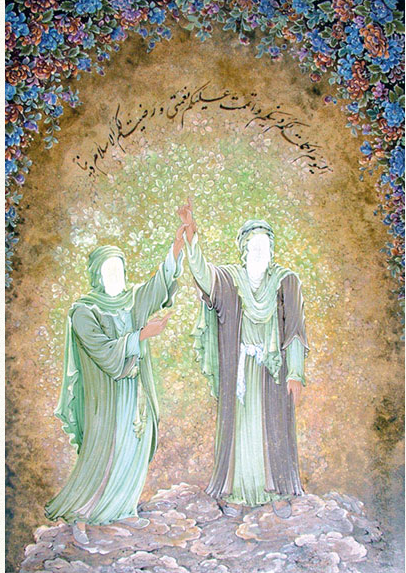
\includegraphics[width=1.35188in,height=1.90972in]{Images/image078.png}
    \caption{Ġadir-e Khumm et la
désignation de l'Imâm `Alī. œuvre de Rezâ
Badr-os-Samâ'}
    \label{Ġadir-e Khumm}
\end{marginfigure}

Il y reçut le verset suivant~: 
\begin{quote}
  {«~O Messager, transmets
ce qui t'a été descendu de la part de ton Seigneur. Si tu ne le faisais
pas, alors tu n'aurais pas communiqué Son message. Et Dieu te protégera
des gens. Certes, Dieu ne guide pas les gens mécréants.~» (Coran,
5:67).}  
\end{quote}


Par la suite, selon les šī`ites, Muḥammad déclara~: «~Man kuntu Mawlāhu,
fahaza `Alī mawlāhu~» c'est-à-dire~: «~Qui me reconnaît comme son Mawlā
(maître, guide), doit reconnaître `Ali comme son Mawlā ~».




Mais pour certains des compagnons du Prophète, cette désignation n'a
jamais été officialisée et selon les mœurs tribales, il convient donc de
procéder à son élection.

Mais `Alī est écarté du collège électoral. \mn{\cite{OUARDI:CalifesMaudits}} 

La tribu des Qurayš élit Abū Bakr, vieux compagnon et un des beaux-pères
de Muhammad~: il devint le 1\textsuperscript{er} calife (khalîfa).

`Alī fera acte d'allégeance, il se soumet à ce choix signifiant son
désir de maintenir l'unité de l'\emph{umma}.

À la mort d'Abū Bakr, `Umar devient le 2\textsuperscript{ème} calife
puisqu'il avait été désigné de manière explicite (\emph{naṣṣ}). `Alī
accepte.

`Umar annonce qu'à sa mort, son successeur devra être choisi parmi les
membres d'un collège électoral qu'il a lui-même nommés. `Alī en fait
partie. À la mort de `Umar, c'est `Uṯmān qui est choisi. Accusé de
népotisme, il est assassiné.

`Alī devient alors le 4\textsuperscript{ème} calife (656-661) attestant
ainsi de ses qualités vertueuses et de la suprématie de l'imamat sur les
manigances politiques mondaines.

Pour autant, deux anciens compagnons du Prophète n'ayant pas vu leur
appétit politique satisfait -- ils souhaitaient être gouverneurs de Kūfa
et Baṣra -- s'associèrent à `Ā'iša, fille d'Abū Bakr et veuve du
Prophète, pour lever une armée contre `Alī. C'est la bataille du chameau
de 657. On l'appelle ainsi parce que `Ā'iša qui était présente, était
montée sur un chameau\ldots{} Son armée fut mise en défaite.





\mn{On voit ici `Ā'iša sur son chameau et dans son baldaquin}



Mais en Syrie, Mu`āwiya, parent de `Uṯmān, mena aussi une guerre. C'est
la bataille de Ṣiffīn. Alors qu'elle tournait à l'avantage de `Alī,
Mu`āwiya proposa un arbitrage sur le livre sacré. `Alī accepte. Nombre
de ses soldats se soulèvent considérant qu'il n'avait pas à accepter
l'arbitrage et que Dieu avait déjà rendu son jugement par la victoire
qui se manifestait. `Alī doit mener combat contre ces rebelles (ce sont
les ḫariǧites), alors que Mu`āwiya se fait proclamer calife à Jérusalem
en 660~!

`Alī est assassiné par un ḫarigite à Kūfa en 661.

Pour les sunnites, il n'avait pas de successeur tandis que les šī`ites
affirment qu'il avait nommé son fils aîné, al-Ḥasān.

 
\subsection{La généalogie du
šī`isme}\label{la-guxe9nuxe9alogie-du-ux161ux12bisme}

La généalogie est sujet à controverses et divergences ce qui explique la
multiplication des šī`ismes\textbf{.} On dénombre une centaine de
lignées à la fin du premier siècle de l'Hégire.

Les jours de naissances des membres de la famille de `Alī sont des fêtes
religieuses. Les jours anniversaires de leur mort, des journées de
deuil. Leurs tombes sont des lieux de pèlerinage~: les cités où elles se
trouvent sont des villes saintes.

Elle est un peu subtile, chaque imām mériterait un chapitre\ldots{}
entre son enseignement, les histoires, les légendes, leur assassinat --
souvent empoisonné -- sans compter qu'au sein même du šī`isme, les
généalogies, les filiations ne sont pas les mêmes, que certains ne
reconnaissent que quatre imāms, d'autres sept, d'autres douze, que ce ne
sont pas toujours les mêmes\ldots{} qu'il y a donc une multitude de
branches šī`ites\ldots{} Bref, je retiens surtout le šī`isme majoritaire
dit duodécimain, car il reconnaît 12 imāms. Vous en trouverez en annexe
la liste avec leurs noms et quelques caractéristiques. Si vous avez la
curiosité de regarder le douzième, vous voyez que n'est pas indiquée la
date de sa mort. D'après vous, est-ce parce que l'on ne la connaît pas,
ou est-ce pour une autre raison~? La réponse dans la suite du cours. Bon
travail.

 
\paragraph{`Alī et Fātima}\label{alux12b-et-fux101tima}

`Alī joue donc dans le šī`isme un rôle important. Il est à la tête de
presque toutes les chaînes de transmission, il est considéré ~comme un
maître spirituel. On lui attribue deux livres~: \emph{Nahj al-balâgha}
(La Voie de la maturité)~et \emph{Dîwân}, un recueil de poèmes.

Quant à Fātima, elle est la sainte la plus vénérée du šī`isme\textbf{.}
Sa tombe est à Médine (il y en a trois\ldots{} dans le doute, on les
garde toutes les trois).

Fātima est la mère de toute la lignée des imāms. Elle représente ce qui
relie Muhammad à `Ali, la lettre et l'esprit. Elle est dite \emph{maǧma`
al-nūrayn} (le Confluent des Deux Lumières), celle de la prophétie et de
l'imamat. Elle a une mission d'intercession et de protection jusqu'à la
fin des temps. Immaculée, Vierge malgré son mariage, elle est aussi
reine du ciel. Un parallèle avec Mariam (Marie), la mère de Jésus est
établi par la tradition šī`ite elle-même \sn{Tahani Sabri,
  «~L'hagiographie de Fāṭima d'après le \emph{biḥār al-anwār}~», École
  des Hautes Études en Sciences Sociales, thèse de doctorat sous la
  direction de Henry Corbin, 1969.}.

 
\paragraph{Al-Hasan, fils de
`Alî}\label{al-hasan-fils-de-aluxee}

C'est un petit-fils du Prophète. Il y a des récits touchant d'affection
tendre.

Al-Ḥasan abdiqua le califat devant l'hostilité de Mu`āwiya. Pour les
historiens šī`ites, il préféra l'unité de la communauté plutôt que de
voir la division, mais les sunnites font remarquer qu'il n'était pas en
mesure de remporter la victoire et qu'il abdiqua en contre-partie d'une
importante somme d'argent. Retiré à Médine, il est assassiné,
semble-t-il par une de ses épouses qui aurait été soudoyée, selon les
šī`ites par Mu`āwiya. Terrible Mu`āwiya\ldots{} J'imagine que vous ne
devez pas le trouver très sympathique. Il est le fondateur de la
dynastie Omeyyade. Les grands historiens sunnites des
8\textsuperscript{ème} et 9\textsuperscript{ème} siècles n'en ont pas
laissé un souvenir très élogieux\ldots{} car ils sont abbassides et il
fallait effacer les traces vénérables des Omeyyades.

 
\paragraph{Al-Ḥusayn} 

Al-Ḥusayn, le second fils de `Alī, reste discret. Il s'efface. Mais il
entre sur la scène politique au moment de la mise en place d'une
dynastie califale héréditaire en la personne de Yazīd, le fils de
Mu`āwiya. On se réfère souvent à lui pour présenter le šī`isme comme un
courant révolutionnaire, politique et contestataire.

L'histoire est plus complexe. En tous les cas, les sources appellent une
très grande prudence. Assuré du soutien de la ville de Kūfa, il se met
en route avec toute sa famille pour chasser les Omeyyades. Mais sur la
route, la petite troupe se trouve encerclée par les soldats omeyyades,
coupée de Kūfa, privée d'eau. Retranchée en plein désert dans un petit
village appelé Karbalā', les Omeyyades finissent par donner l'assaut.
C'est un massacre. Ḥusayn est tué, décapité, piétiné ainsi que quasiment
toute sa famille.

Ašura est le jour de célébration où l'on fait mémoire de cette tragédie
dans de grandes cérémonies populaires avec parfois des dérives
spectaculaires de lamentations violentes, d'auto-flagellations, de
lacérations ou de mutilations. C'est le remord d'une ville qui n'a pas
soutenu al-Ḥusayn.

Ḥusayn devint alors un exemple de martyr, de sacrifice, de bravoure.
Sans-doute, sous l'influence chrétienne, on verra dans la mort de Husayn
un sacrifice rédempteur pour le salut des fidèles.

Chez certains fidèles la rumeur selon laquelle il ne serait pas mort
circule. Il aura été enlevé au ciel directement par Dieu avant le
combat.


\mn{Les troupes omeyyades encerclent Karbalā' \& Yā Ḥusayn\ldots{}

Jour de la fête d'Ashura \& Ashura et ses spectaculaires flagellations à
Karbalā'\ldots{} }


 
\paragraph{`Alî Zayn al-`Âbidîn, fils
d'al-Husayn}\label{aluxee-zayn-al-uxe2biduxeen-fils-dal-husayn}

Un rescapé du massacre de Karbalâ'. Il serait parti à Médine pour y
mener une vie pieuse. Il ne posa aucun problème aux Omeyyades. Une
existence ascétique, consacrée à la dévotion. On le surnommait
\emph{al-saǧǧād}, celui qui accomplit de nombreuses prosternations.
C'est un nom respecté, même dans le sunnisme.

Un de ses fils Zayd ibn `Alî, est à l'origine d'une grande famille, les
zaydites. Le zaydisme est marqué par un activisme violent. Selon la
théorie zaydite de l'imamat chaque Alide a le droit de prétendre à la
direction de la communauté. Le véritable imâm est celui qui se qualifie,
les armes à la main, en s'insurgeant contre le pouvoir injuste. Ils sont
aujourd'hui encore influents au Yémen~où ils représentent la moitié de
la population (mais le dernier chef zaydite du Yémen a été renversé en
1962).

 
\paragraph{Muhammad al-Bāqir, fils de `Alî Zayn
al-`Âbidîn}\label{muhammad-al-bux101qir-fils-de-aluxee-zayn-al-uxe2biduxeen}

Il est considéré comme le fils de `Ali Zayn. Les grandes traditions
šī`ites le considèrent comme le 5ème Imām. Il est surnommé Abū Ǧa`far.

 
\paragraph{Ǧa'far al- Ṣādiq
}\label{ux1e7afar-al--ux1e63ux101diq}

Fils de Muhammad al-Bāqir, il est célèbre pour sa piété et, selon les
shiites, l'infaillibilité de ses prémonitions. Les auteurs soufis lui
attribuent le plus ancien commentaire mystique du Coran. On le considère
comme un alchimiste, un spirituel refusant toute implication dans les
mouvements politiques de son époque. Il fut enterré dans le cimetière de
Baqī` à Médine. Le carré šī`ite y sera rasé au XIX° siècle par les
Wahhabites, alors qu'il abritait les tombes de plusieurs imâms.

Son fils aîné, Ismā`īl, est l'éponyme de la seconde grande famille de
l'islam šī`ite, les ismaéliens, šī`ites septimains \textbf{--} shî'ites
à 7 imâms. Pour cette branche, il est le dernier Imâm. Un autre groupe
s'appuie sur la croyance que l'imamāt fut transmis du vivant de Ǧa`far à
son petit-fils~: ce sont les qarmates. D'autres, les Fatimides,
considèrent que l'imamat se poursuit et que l'imam caché, le Mahdi, sera
un de ses descendants.


\begin{Synthesis}
Le si'isme est  une prophétologie. Il y a une sur
l'incarnation. Facilite le
dialogue avec les chrétiens.
\end{Synthesis}

 
\paragraph{{Le douzième imām, l'imām caché ou
le Madhī
}{ }}\label{le-douziuxe8me-imux101m-limux101m-cachuxe9-ou-le-madhux12b}

À la mort du 11\textsuperscript{ème} imâm, les fidèles croient que
l'imâm a eu un fils du nom de Muḥammad. 
\begin{Def}[Mahdî]
Il est reconnu comme le
\emph{Mahdî,} le Bien Guidé. C'est l'imâm caché, \emph{al-imâm al-ġā'ib}
ou encore \emph{al-Qā'im}, que l'on peut traduire par le Résurrecteur.
\end{Def}


C'est le courant duodécimain, majoritaire dans le šī`isme.

Mais en quoi consiste cette occultation~? Comment s'opère-t-elle~? Que
signifie-t-elle~? Quand a-t-elle eu lieu~? Sous quelles formes~?

Je vous propose d'écouter ce bref passage d'une émission sur France
Culture, «~Les racines du ciel~», où Amir-Moezzi répond.

L'imâm caché n'est donc pas mort. Vous comprenez maintenant pourquoi
dans le tableau en annexe ne figure que sa date de naissance. Il
n'existe pas de successeur puisqu'il est physiquement vivant. À la fin
des temps, il se manifestera. Il y a donc une présence invisible, mais
physiquement réelle. L'imâm caché clôt la lignée des imamites.

Par la suite, tout se passe comme si désormais l'ère de la bonne entente
entre le religieux et le politique était désormais finie. La cité
idéale, gouvernée par un juste n'est réalisable qu'à la fin des temps,
avec l'avènement du Mādhi, le Sauveur eschatologique. L'attitude
revendicative et politique est rejetée dans un futur messianique. Le
šī`isme se présente comme une religion individuelle, personnelle, non
institutionnelle. Mais peut-il alors perdurer ? Pour pallier cette
«~absence~», on aura recours à la figure du juriste avec la dynastie
bouyide. C'est à cette époque que le šī`isme sera érigé comme religion
d'État, ce qui n'est pas le moindre des paradoxes compte tenu de ses
«~fondamentaux~».

 
\section{Les fondations du šī`isme~:
doctrines}\label{ii.-les-fondations-du-ux161ux12bisme-doctrines}

Les doctrines šī`ites sont compliquées, subtiles et à lire
l'enseignement des imāms et les commentaires qui en suivirent, cette
subtilité est voulue pour elle-même. De leurs enseignements, ils ne
cessent de dire~: «~notre enseignement est ardu, difficile à supporter~:
c'est un secret, un secret enveloppé par un secret au sujet d'un
secret~»\sn{Voir Amir-Moezzi, Jambet, \emph{Qu'est-ce que le
  shi'isme~?}, Paris, Fayard, p. 96 .}.

Dans sa présentation du šī`isme, Amir-Moezzi distingue dans la vision du
monde et la théologie šī`ite une double dimension~: elles sont marquées
à la fois par l'affirmation d'un principe de dualité et d'un principe de
dualisme. On lira avec intérêt et pour plus de précisions la
présentation qu'il fait dans \emph{Qu'est-ce que le shiisme~?} Mais tout
d'abord, la question des Écritures. Sont-elles les mêmes qu'en
sunnisme~?

 
\subsection{{Les sources scripturaires
}}\label{les-sources-scripturaires}

 
\paragraph{{Y a-t-il un Coran šī`ite~?
}}\label{y-a-t-il-un-coran-ux161ux12bite}

Le Coran est la référence principale et la contradiction éventuelle
entre un \emph{ḥadīṯ} et un verset coranique est l'indice de la fausseté
du ḥadīṯ.

Pour autant, certaines traditions shî'ites trouvent difficilement leur
fondement dans le Coran. Pour les šī`ites, le Coran a été en réalité
falsifié, altéré, censuré lors de sa compilation par `Uṯmān (c'est un
des premiers califes. Si le nom ne vous disait plus rien du tout,
revoyez le premier cours sur le Coran et à la question du
\emph{muṣhaf}). La révélation originelle contenait des versets sur `Alî
et les descendants des Prophètes. Ils étaient cités comme les modèles et
les chefs par excellence. `Alī possédait une version du Coran intégral,
mais il n'en dit mot pour éviter sa destruction par ses adversaires.
Cependant, elle fut transmise secrètement d'imam à imam, jusqu'au
12\textsuperscript{ème} imâm qu'il l'emporta avec lui lors de son
Occultation. Les enseignements des imāms permettent d'accéder à ces
versets et de les connaître.

Avec l'arrivée au pouvoir des Bouyides shiites à la fin du
4\textsuperscript{ème} siècle de l'hégire, il s'agira de trouver un
accord avec l'orthodoxie sunnite. On met ainsi un terme au doute sur
l'intégrité du Coran officiel. Le courant dominant abandonne la thèse de
la falsification du Coran officiel, mais le débat ressurgit
régulièrement.

 
\paragraph{Y a-t-il un \emph{ḥadīṯ} šī`ite~?
} 

Bien qu'al-Būḫārī fut perse, il existe une Sunna šī`ite. Les textes sont
bien souvent les mêmes, mais les \emph{isnāds} diffèrent et renvoient
aux membres de la famille du prophète (\emph{ahl al-bayt} --
c'est-à-dire littéralement, les gens de la maison). En effet, la
référence dans l'\emph{isnād} aux compagnons du Prophète lui ôte toute
crédibilité dans la mesure où ils sont considérés comme des traîtres.
Pour l'\emph{isnād}, la notion a été vue dans le cours sur la Sunna.
C'est la fameuse chaîne de transmission.

On reconnaît trois grands corpus~:

\begin{itemize}
\item
  Celui de Ya`qub al-Kulaynī (m. en 939).
\item
  Celui de Saduq Ibn Babuyeh (m. 991).
\item
  Celui d'al-Ḥasan al-Tusī (m. 1068).
\end{itemize}

On trouve aussi dans ces recueils de nombreux témoignages des imāms.

L'ouvrage le plus connu de Kulaynī est \emph{al-Kāfī}. Il est divisé en
trois sections~:

\begin{itemize}
\item
  \emph{Usūl al-Kāfī}, qui concerne l'épistémologie, la théologie, la
  question de la foi et de la mécréance, l'histoire, l'éthique, et le
  Coran~et ses mérites;
\item
  \emph{Furūʿ al-Kāfī}, qui concerne les dimensions pratiques et légales
  (prières, \emph{ǧihād}, jeûne, ḥaǧǧ, funérailles, nourriture, boisson,
  mariage, divorce, commerce, héritage, etc.)
\item
  \emph{Rawdat} \emph{al-Kāfī}, qui inclue de nombreuses traditions, des
  lettres, des discours des imāms.
\end{itemize}

Il existe une traduction anglaise de cette collection de plus de 16 000
traditions. Si vous ne trouvez pas le sommeil\ldots{}
 
\subsection{ Dualité et dualisme}\label{dualituxe9-et-dualisme}

 
\paragraph{ Une vision duelle}\label{une-vision-duelle}

Il s'agit d'affirmer que toute réalité possède deux niveaux~:

1/ un niveau manifeste, obvie, apparent, visible, concret, évident
(\emph{zāhir})

2/ un niveau secret, non manifeste, implicite, invisible, intérieur
(\emph{bāṭin})

Cette affirmation est au cœur du credo šī`ite. Ce que je vois, ce qui
est visible contient aussi une réalité invisible. Il existe une relation
entre le manifeste et le caché, l'exotérique et l'ésotérique. Il s'agit
d'appliquer ce principe à toute réalité, et bien sûr, à commencer par la
théologie.

\emph{Ainsi, en théologie}, Dieu a deux niveaux d'être, deux niveaux
ontologiques~:

1/ son Essence, inconcevable, inimaginable, au-delà de toute pensée~:
c'est le niveau caché (\emph{bāṭin})

2/ ses Noms et Attributs~à travers lesquels Dieu se révèle et se fait
connaître~: c'est le Dieu inconnu qui aspire à être connu. Amir-Moezzi
remarque que l'on retrouve une distinction de la théologie médiévale
chrétienne entre \emph{Deus absconditus} et \emph{Deus revelatus}.

La manifestation de ces noms divins comme le Roi, le Miséricordieux, le
Juge suprême, etc. est une manifestation de Dieu (théophanie). La plus
haute révélation en est la figure de l\emph{'Imām} céleste,
l'\emph{Imām} de Lumière, l'Homme cosmique~: c'est l'Imām avec un I
majuscule, dans son acception ontologique universelle.

L'\emph{Imām} cosmique a aussi deux dimensions

\begin{quote}
1/ la dimension cachée~: c'est l'aspect métaphysique, dans le ciel,
invisible à nos yeux.

2/ la dimension exotérique, visible~: ce sont les \emph{imāms}
historiques.
\end{quote}

La mission de ces \emph{imāms} historiques~consiste à dévoiler les
mystères de Dieu, du monde et de l'homme, à transmettre aux hommes le
Secret contenu dans l'Imām métaphysique.

Mais l'enseignement des imāms, disions-nous, est complexe. Ǧa`far
al-Ṣādiq (c'est un \emph{imām} que nous avons rencontré dans la
généaologie des douze\ldots{} C'est le combientième \emph{imām} déjà~?)
écrivait~: «~Notre enseignement comporte l'exotérique, l'ésotérique et
l'ésotérique de l'ésotérique~».

À cette approche duelle de la réalité se superpose le principe du
dualisme.

 
\paragraph{ Une vision dualiste}\label{une-vision-dualiste}
\mn{Si isme~: influence de la zoroastrisme avec un certain manichéisme, bien
/ mal. Lumière et nuit~; combat cosmique et sur terre. On retrouve ceci
dans le sunnisme. Tous les Hadiths eschatologiques décrivent en tableau
le paradis. Dans le Si isme, enjeu du bien et du mal.
}
L'histoire de la création est celle d'un combat cosmique entre les
forces du Bien et les forces du Mal, entre la lumière et l'obscurité. On
retrouve ici une nette dimension zoroastrienne et manichéenne du monde.

Ce combat se situe au niveau cosmique~: c'est le combat entre les armées
de l'Intelligence cosmique (\emph{al-`aql}) et celles de l'Ignorance
cosmique (\emph{al-ğahl}). Cette dichotomie, cette opposition est celle
d'une lutte permanente entre les Gens de la Droite (\emph{ašāb
al-yamīn}) et les gens de la Gauche (\emph{ašāb al-šimāl}). Le combat
entre deux hommes ennemis s'inscrit donc dans un cadre plus large. Toute
l'histoire de l'humanité est traversée par l'adversité et la violence
des forces démoniaques de l'Ignorance. Il en sera ainsi jusqu'à la fin
des temps avec l'avènement du Sauveur eschatologique, le Mahdī qui
vaincra définitivement les forces du mal.

Mais qui sont ces forces du mal~? Comment les reconnaître, les
identifier~?

C'est l'enseignement des imāms (les 7, les 12, selon) qui apportent les
réponses à ces questions. Dans ce corpus de centaines de milliers de
pages, les adversaires de l'imâm~sont tour à tour identifiés~:

\begin{itemize}
\item
  Aux juifs, qui sont des idolâtres et ont trahi Moïse en adorant le
  veau d'or
\item
  Aux Compagnons de Muhammad qui ont rejeté `Alī
\item
  Aux Gens de l'exotérique, c'est-à-dire des apparences, du superficiel
  (\emph{ahl al-zāhir}), ce sont les littéralistes qui s'arrêtent à la
  lettre et n'ont pas connaissance de son `esprit' (\emph{bāṭin}). À cet
  égard, un šī`ite se sentira plus proche d'un juif ou d'un chrétien
  accoutumé à une lecture ésotérique, symbolique, anagogique des textes
  que d'un musulman sunnite exotérique, qui se limite à la lettre.
\end{itemize}

 
\subsection{Prophétie et
Imamologie}\label{prophuxe9tie-et-imamologie}

L'enseignement des \emph{imāms}, acquiert en réalité un rôle supérieur à
celui du Prophète.

En effet, si le prophète est le messager de la lettre, l'\emph{imām}
dans le šī`isme en apporte l'esprit. Or, si l'esprit peut exister sans
la lettre, sans l'esprit, la lettre est morte\sn{Amir-Moezzi,
  Jambet, \emph{Qu'est-ce que le shi'isme~?}, Paris, Fayard, 2004, p.
  42.}.


\paragraph{Remarque sur l'imām~}: le mot \emph{imām}
est piégé. Il s'emploie en sunnisme, mais sans désignation particulière.
L'imām désigne un savant, un chef ou tout simplement celui qui dirige la
prière. En revanche, en šī`isme\textbf{,} c'est un titre sacré. L'imām
est le Guide, l'un des Douze\ldots{} En principe, aucun autre homme ne
porte ce nom. Et pourtant, d'aucuns se sont attribués ce titre. Autant
dire qu'ils se prenaient pour le Mahdi .L'un d'eux est très célèbre. À
suivre.

L'Imām apporte en effet la connaissance face au monde de l'ignorance. En
montrant son cœur, l'Imām `Alī donnait cet enseignement sur la vocation
de l'imām, la nature de la religion, son importance. Écoutez et
réécoutez ce texte\sn{Vous trouvez l'intégralité du texte dans le
  livre de Mohammad Ali Amir-Moezzi, \emph{La religion discrète}, Paris,
  Vrin, 2006,
  \url{https://books.google.com}}.


L'imām transmet les vérités secrètes. Il tient le monde, il évite la
noyade définitive du monde dans les ténèbres. Il est l'alpha et l'omega
du šī`isme\sn{Amir-Moeezi, Jambet, \emph{Qu'est-ce que le
  shi'isme~?}, p. 40.}.

Mais il a aussi des pouvoirs supra-normaux~: il possède la science du
passé et du futur, il lit dans les consciences, il connaît les langues,
y compris celle des animaux, les sciences occultes (astrologie,
alchimie, sciences divinatoires, etc.). Il peut ressusciter les morts,
guérir les maladies, rajeunir les vieillards, marcher sur les eaux,
monter aux cieux\ldots{} Il possède des objets de pouvoir~ tels la
tunique d'Adam, le sceau de Salomon, l'Arche et les tables de la Loi,
l'Arme invincible de Muḥammad.

L'enseignement de l'\emph{imām} est au cœur de l'approche spirituelle
šī`ite. C'est par lui que se réalise la spiritualisation, la
divinisation. Écoutez Amir-Moezzi à ce sujet.

 
\subsection{La walāya au cœur de la foi šī`ite
} 


La \emph{walāya} est un concept clé du \emph{šī`isme}. Les
\emph{šī`ites} sont appelés les gens de la \emph{walāya}.\\
\begin{Def}[walāya]
La \emph{walāya} désigne la mission sacrée et sainte des imams.

L'imām est le \emph{walī} (le saint), celui qui initie les fidèles à
l'esprit de la Parole divine. Il est la Face de Dieu sur terre.

\end{Def}



La \emph{walāya} désigne aussi l'amour, celui que les fidèles
manifestent dans la dévotion, par la loyauté, la soumission à l'égard du
maître initiateur.

Mais dans une doctrine \textbf{dualiste}, l'amour de l'imām ne peut aller sans la
haine de son ennemi. La \emph{walāya} est donc inséparable de son
contraire, la \emph{barā'a} (c'est-à-dire la haine, la dissociation à
l'égard des forces de l'ignorance). Un \emph{ḥadīṯ} šī`ite dit~:

\begin{quote}
«~l'amour de Dieu ne s'obtient que grâce à l'amour envers Ses amis et
l'hostilité à l'égard de Ses ennemis~».    
\end{quote}


Au cœur de la foi šī`ite, la \emph{walâya} est dans la \emph{šahāda} :
\begin{quote}
   «~Je témoigne qu'il n'y a pas de dieu hormis Dieu~; je témoigne que
Muhammad est l'envoyé de Dieu, et que `Alî est le \emph{walī} de
Dieu~» 
\end{quote}
 \emph{walī} signifie ici l'ami,~l'allié, le détenteur de la
\emph{walāya}.




\mn{\emph{Šahāda} sur une mosquée du Caire
fatimide. on y lit à la fin~:\emph{ʿAlī walī
allāh.
}  }


\subsection{{Les signes de la fin du monde ou
l'eschatologie šī`ite
}\label{les-signes-de-la-fin-du-monde-ou-leschatologie-ux161ux12bite}}

En raison de la place de la question de l'Occultation, l'eschatologie a
donné lieu à un foisonnement de traditions et de traités. Il s'agit de
savoir lire les signes afin de reconnaître l'imminence du Dernier Jour,
le retour du Mahdī. Les signes sont multiples, mais on peut identifier
quelques constantes~:

\begin{itemize}
\item
  l'envahissement de la terre par les forces du Mal,
\item
  l'écrasement quasi-complet des forces de la Connaissance par celles de
  l'ignorance,
\item
  la perte du sens du sacré,
\item
  le renversement des valeurs humaines,
\item
  l'anéantissement de tout ce qui relie l'homme à Dieu et à son prochain
\end{itemize}

Des signes concrets sont exposés. Ainsi par exemple,

\begin{itemize}
\item
  la venue d'al-Sufyānī, le chef de l'armée des ennemis des imāms, le
  collaborateur d'\emph{al-Daǧǧāl}, l'Imposteur, l'Antéchrist islamique.
\item
  L'avènement d'al-Yamānī, le Yéménite qui prêchera le soutien au Mahdī.
\item
  Le Cri, d'origine surnaturelle, venu du ciel, appelant les hommes à
  rejoindre l'armée du Sauveur
\item
  L'engloutissement d'une armée (parfois celle d'al-Sufyānī) dans le
  désert.
\item
  L'assassinat à La Mecque de l'envoyé du Mahdī, appelé \emph{al-Nafs
  al-Zakiyya\textbf{~}}: l'Âme Pure.
\end{itemize}

La fin de l'occultation est aussi expliquée et commentée. On peut en
distinguer 3 raisons~principales :
\begin{enumerate}
    \item une raison historique~: venger tous les hommes saints du passé,
victimes de l'injustice. Tous les saints du passé reviendront à la vie,
ainsi que leurs meurtriers, et les premiers pourront ainsi se venger des
seconds à cette occasion.
\item une raison religieuse~: rétablir le sens du sacré~; rétablir les
religions (judaïsme, christianisme, islam) dans leur intégralité
originelle, rapporter les Écritures respectives qui ont été altérées ou
falsifiées
\item une raison spirituelle~: apporter le sens ésotérique des choses,
effacer la frontière entre le caché et le manifeste.
\end{enumerate}
 

Le retour du Mahdi s'accompagne aussi de celui de Jésus-Christ. Il est
le principal compagnon d'al-Qā'im. Voyez un peu plus haut. C'est un nom
utilisé pour nommer le Mahdi. Quelle est sa signification déjà~? Penser
à «~\emph{Talitha Qum~}».. Lève-toi\ldots{} C'est bien la même racine du
redressement, de la résurrection.

 
\section{Bibliographie}\label{bibliographie}

\paragraph{Les fondamentaux}

Mohammad-Ali \textsc{Amir-Moezzi}, Christian Jambet, \emph{Qu'est-ce que
le shî'isme~?,} Paris, Fayard, 2004.

Henri \textsc{Corbin}, \emph{En Islam iranien}, Aspects spirituels et
philosophiques III, Les Fidèles d'amour, shî'isme et soufisme,
Gallimard, 1978, 359 pages (PISAI H266).

\paragraph{Pour aller plus loin}

Mohammad Ali \textsc{Amir-Moezzi}, \emph{La religion discrète},
Croyances et pratiques spirituelles dans l'islam shî`ite, Collection
Textes et Traditions dirigée par Marie-Odile Goulet-Cazé, Richard
Goulet, Philippe Hoffmann, Paris, Vrin, 2006.

Henri \textsc{Corbin}, «~De l'histoire des religions comme problème
théologique~», \emph{Monde non chrétien} 51-52, 1960

Leili \textsc{Echghi}, \emph{Un temps entre les temps~: L'Imam, le
Chî'isme et l'Iran}, coll. Patrimoines Islam, cerf, Paris, 1992.

Geneviève Gobillot, \emph{Les Chiites}, Editions Brepols, 1998.

Henri Laoust, \emph{Comment définir le sunnisme et le chiisme},
Geuthner, 1985, 44 pages.

Muhammad Ridā Muzaffar, \emph{Le credo des imamites}, traduction par
Frère Sliwa, Rome, PISAI.

Yann \textsc{Richard}, \emph{Le Šī`isme en Iran~: Imam et Révolution,
Librairie d'Amérique et d'Orient}, 1980, 142 pages.

Yann \textsc{Richard}, \emph{L'islam chi'ite~: croyances et idéologies},
Fayard, Paris, 1991.

\textbf{\hfill\break
}

\subsection{Généalogie des Imāms}


 

\begin{longtable}{p{0.5cm}p{1.3cm}p{1.8cm}p{2.5cm}p{3.5cm}p{0.8cm}}
\small \\
%\sidecaption{Généalogie des Imāms} \label{tab:Genealogie} \\
\toprule
 & Nom & Titre & Epithète & connu pour & dates
\\
\midrule
\endhead
1 
& 
\vtop{{ `Alī}{ (\TArabe{علي})}} 
&
\vtop{{ Abū al-Ḥassan}{ (\TArabe{أبو الحسن})}}
&
\vtop{{ Amīr al-Mu'minīn}{ (\TArabe{أمیر المؤمنین}) -
Commandeur des croyants}} 
& Le premier Imam est la personne la plus
significative après Mahomet pour les chiites 
& 600 -- 661 \\



2 & \vtop{{ Ḥasan}{ (\TArabe{ألحسن})}} &
\vtop{{ Abū Muḥammad}{ (\TArabe{أبو محمد})}} &
\vtop{{ Al-Mujtabā}{ (\TArabe{ألمجتبی}) - le choisi}}
& Signe un traité de paix pour un Islam meilleur, très aimé par Mahomet
est avec son frère un des maîtres des jeunes du paradis & 625 -- 669 \\


3 & \vtop{{ Ḥusayn}{ (\TArabe{ألحسین})}} &
\vtop{{ Abū \textsuperscript{c}Abdillāh}{ (\TArabe{أبو
عبداللھ})}} & \vtop{{ Sayyid
ash-Šuhadā'}{ (\TArabe{سید الشھداء}) - Seigneur des martyrs}} &
Est mort lors de la bataille de Kerbala. & 626 -- 680 \\


4 & `Alī (\TArabe{علي}) & \vtop{{ Abū
Muḥammad}{ (\TArabe{أبو محمد})}} & \vtop{{ Zayn
al-\textsuperscript{c}Ābidīn}{ (\TArabe{زین العابدین}) - Joyau
des croyants}} & Piété, jeûne, pénitence pendant 20 ans à cause de la
bataille de Kerbala. & 658 -- 713 \\


5 & Muḥammad (\TArabe{محمد}) & \vtop{{ Abū
Ja\textsuperscript{c}far}{ (\TArabe{أبو جعفر})}} &
\vtop{{ Al-Bāqir}{ (\TArabe{ألباقر}) - Pourfendeur de
la Science}} & le moins oppressé des douze imams par le calife de son
temps. Il n'est pas reconnu par les Zaydī (qui prennent comme imam Zayd
Ibn `Alī. & 676 -- 743 \\


6 & \vtop{{ Ǧa'far}{ (\TArabe{جعفر})}} &
\vtop{{ Abū \textsuperscript{c}Abdillāh}{ (\TArabe{أبو
عبداللھ})}} & \vtop{{ Aṣ-Ṣādiq}{ (\TArabe{ألصادق}) -
Le véridique}} & Un penseur respecté à la fois par les Chiites et les
Sunnites & 703 -- 765 \\


7 & \vtop{{ Mūsā}{ (\TArabe{موسی})}} &
\vtop{{ Abū Ibrāhīm}{ (\TArabe{أبو إبراھیم})}} &
\vtop{{ Al-Kāẓim}{ (\TArabe{ألکاظم}) - Le triste}} & A
grandi en prison pour le rendre faible Il n'est pas reconnu par les
ismaéliens & 745 -- 799 \\


8 & \vtop{{ `Alī}{ (\TArabe{علي})}} &
\vtop{{ Abū al-Ḥassan}{ (\TArabe{أبو الحسن})}} &
\vtop{{ Ar-Riḍā}{ (\TArabe{ألرضا})}} & Le seul Imam à
être enterré en Iran & 765 -- 818 \\


9 & Muḥammad

(\TArabe{محمد}) & \vtop{{ Abū
Ja\textsuperscript{c}far}{ (\TArabe{أبو جعفر})}} &
\vtop{{ At-Taqī}{ (\TArabe{ألتقي})}} & Un grand
débatteur & 810 -- 835 \\


10 & \vtop{{ `Alī}{ (\TArabe{علي})}} &
\vtop{{ Abū al-Ḥassan}{ (\TArabe{أبو الحسن})}} &
\vtop{{ Al-Hādī (\TArabe{ألھادي}),}{ an-Naqī
(\TArabe{ألنقي})}} & & 827 -- 868 \\


11 & Ḥasan (\TArabe{ألحسن}) & \vtop{{ Abū
Muḥammad}{ (\TArabe{أبو محمد})}} &
\vtop{{ Al-\textsuperscript{c}Askarī}{ (\TArabe{ألعسکري})}}
& L'avant-dernier imam, qui a vécu presque toute sa vie assigné à
domicile et qui prêchait tout de même. & 846 -- 874 \\


12 & Muḥammad

(\TArabe{محمد}) & \vtop{{ Abū Qāsim}{ (\TArabe{أبو
قاسم})}} & \vtop{{ Al-Mahdī}{ (\TArabe{ألمھدي})}} &
Imam actuel, connu pour être le Sauveur. Il est l'occultation. & 868
-- \\
\bottomrule
\end{longtable}

\chapter{Le chiisme : histoire et doctrines}

\mn{21/3/22}
\section{bibliographie}
 

\begin{quote}
AMIR-MOEZZI, M-A. \emph{La religion discrète : croyances et pratiques
spirituelles dans l'Islam shi'ite}, Vrin, Paris, 2006.

AMIR-MOEZZI, M-A. et JAMBET, Christian \emph{Qu'est-ce que le shî'isme
?}, Fayard, Paris, 2004.

CORBIN, Henry \emph{En islam iranien: aspects spirituels et
philosophiques,} 4 volumes, Gallimard, Paris, 1991.

HALM, Heinz \emph{Le Chiisme}, Paris, PUF, 1995.

RICHARD, Yann \emph{L'islam chi'ite : croyances et idéologies}, Fayard,
Paris, 1991.

*TABATABA'I, Muhammad Huseyn \emph{Le chiisme en islam}, Beyrouth,
Al-Bouraq, 2009.
\end{quote}


\section{Le chiisme dans l'histoire
  musulmane. Quelques grands
  repères.}
  \label{le-chiisme-dans-lhistoire-musulmane.-quelques-grands-repuxe8res.}

On aurait pu traiter le développement du Chiisme et du sunnisme car ils ne se développent pas en vase clos. Mais il y a de tels différences,  en particulier, il n'y a pas de \textsc{foisonnement des visions dans le chiisme} du fait de l'importance des clercs
  

 \subsection{La naissance du chiisme : un problème de succession}
 ALi est le gendre et cousin du Prophète.
 
 Ali gagne à sa cause les nouveaux convertis (Egypte, Irak,...) et deviennent partisans d'Ali. Lorsque le Usman est assassiné en 656, Ali est élu comme 4ème calife. 
 \begin{Def}[ahl al-bayt]
\emph{famille du Prophète (Mahomet, Ali, Fatima, Hasan,
Hoseyn)}
 \end{Def}
 
 \paragraph{Mu'awiyya }Mais il est contesté par Mu'awiyya, qui lui reproche de ne pas chercher le meurtrier de Osman. En 657, bataille de Siffin, où les deux parties du monde arabe s'affrontent. Les Khalijites sont ceux qui reprochent à Ali d'avoir accepté l'arbitrage qui suit la bataille de Siffin.
 Ali est assassiné. Le califat est récupéré par Mu'awiyya.
 
 \paragraph{fondation de la dynastie des Omeyyades} par Mu'awyya. Hussayn, second fils de Ali s'oppose à Mu'awyya et est massacré dans la \textsc{plaine de Kerbala} avec sa famille et ses partisans. C'est le traumatisme fondateur. Le 10ème jour (Ashoura) du mois de Muharram, on rappelle ce martyr.
 
 \paragraph{une mosaique de courants shiites autour de la succession de l'imam et sur sa nature}
 Aujourd'hui, il y a trois courants : 
 \begin{itemize}
     \item ismaeliens :  7 imams
     \item zaydites : reconnaissent 5 imams
     \item imamites ou duodécimains : reconnaissent 12 imams.
 \end{itemize}
 
 Le Mahdi\sn{le Mahdi est aussi présent dans le sunnisme mais on ne sait pas qui c'est. Moins d'attente} n'est pas mort, il est occulté mais selon les courants, ce n'est pas le même. 
 
 \begin{Def}[mahdi]
   \emph{« le voilé » : l'homme mystérieux qui viendra annoncer et
provoquer la fin des temps (= dernier imam (occulté) pour les chiites).}
 \end{Def}
 
 \paragraph{Vision eschatologique forte dans le chiisme} Lutte du dernier imams contre le Dajjal, équivalent de \textit{l'antéchrist.}. Cela donne un potentiel révolutionnaire, avec certaines personnes se proclamant \textit{mahdi}, avec un potentiel mobilisateur très puissant, généralement révolutionnaire, voulant renversé le pouvoir établi, avec une forte dimension de justice sociale.
 
 
 
 %-------------------------------------------------
 \subsection{ « Le siècle chiite » : Bouyides et Fatimides (Xe-XIe s)}
 
 
 \paragraph{Diffusion du Chiisme à la mort de Hussayn} Dans les classes pauvres. En Irak par exemple, une grande révolte au IX ème siècle, se réclamant du chiime
 
 \paragraph{les bouyides} dans l'empire Abassides au X-XI, les Bouyides utilisent la faiblesse du calife pour s'imposer comme vizir, qui concentre la réalité du pouvoir : de 975, pendant environ un siècle.  
 
 \begin{figure}
     \centering
 
     \sidecaption{Source: \emph{Historical Atlas of Islam}, Malise Ruthven \& Azim Nanji,
Harvard University Press, 2004, p. 42.}
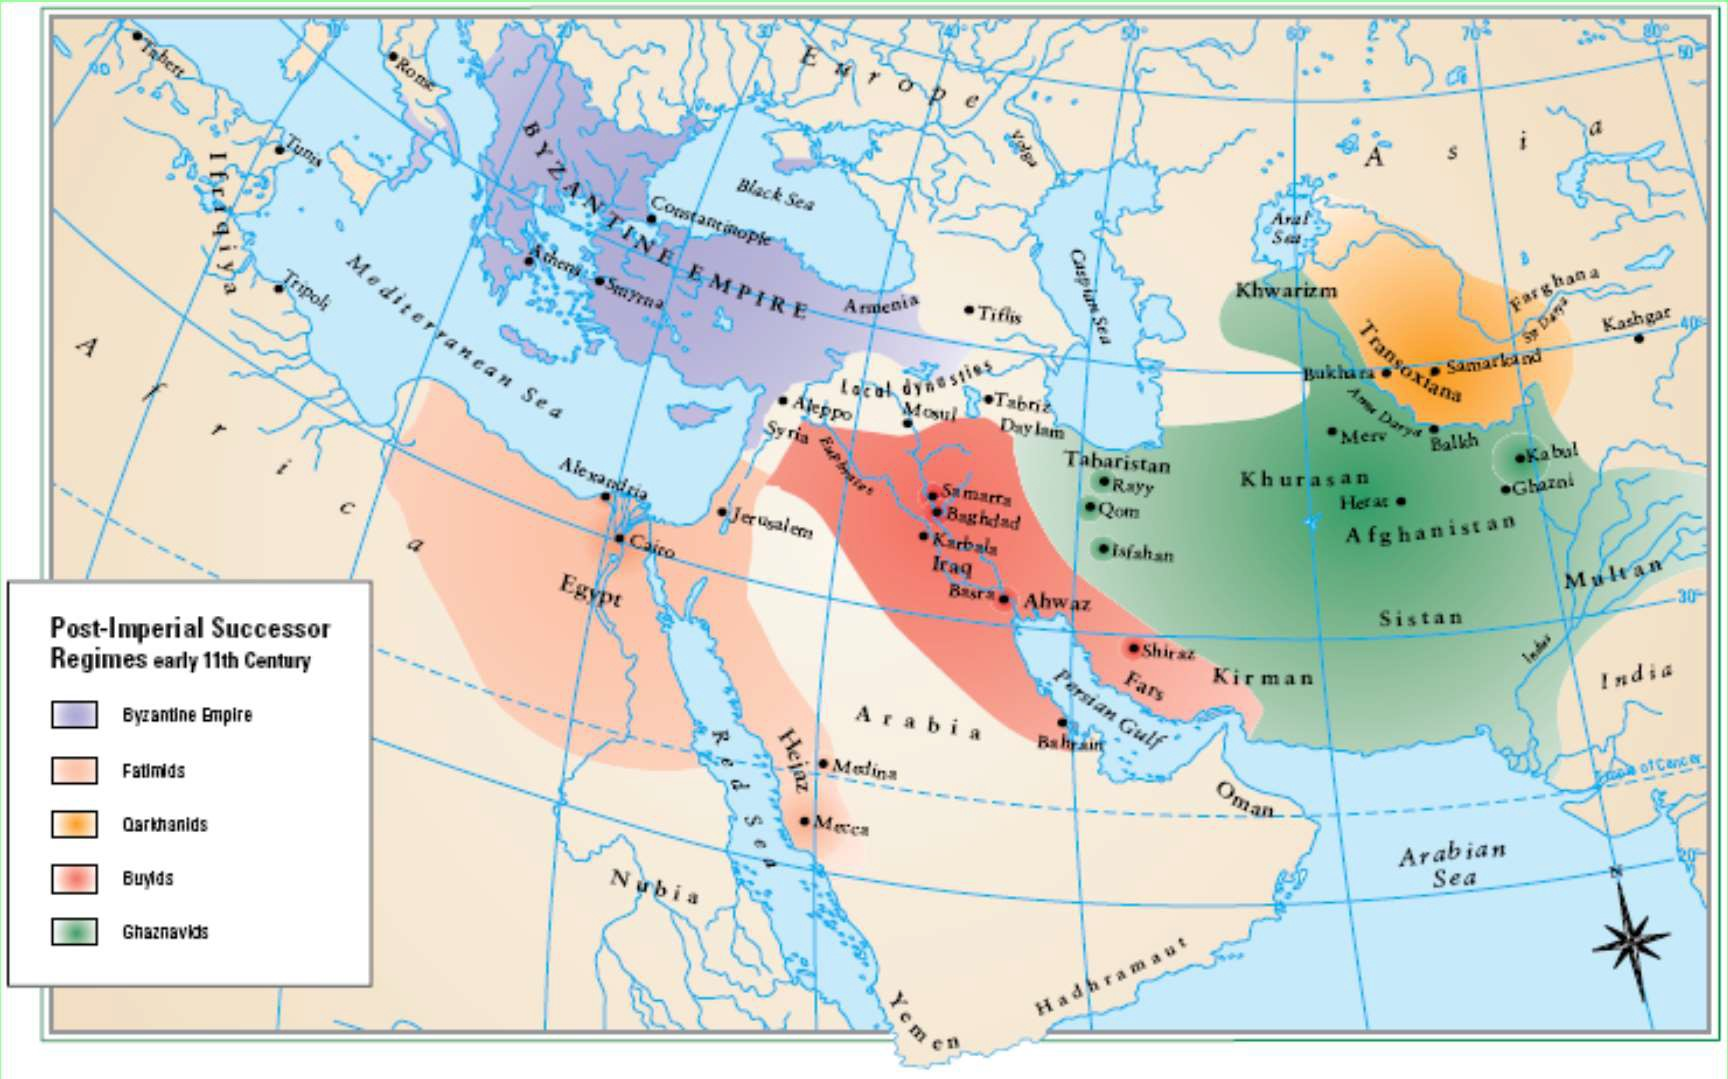
\includegraphics[width=\textwidth]{CourantsIslamContemporain/ImagesCourantsIslamContemporain/Image1Chiisme.jpeg}

     \label{fig:my_label}
 \end{figure}
 
 \paragraph{les fatimides} en afrique du Nord, fondé  par `Ubayd Allâh al-Mahdî (881-934). Typiquement, une personne se déclare Mahdi en Tunisie puis s'empare de l'Egypte (973 : le Caire comme capital). Avant le Caire n'était qu'une ville de garnison. 
 
 \paragraph{à Oman et au Yemen} AU Yémen, Zaydites, de 897 à 1962.
 
 
 %-------------------------------------------------
 
  \subsection{La naissance de l'Iran safavide (XVIe s.)}
 
  \begin{figure}
     \centering
 
     \sidecaption{Source: \emph{l'Iran safavide- Wikipedia}}
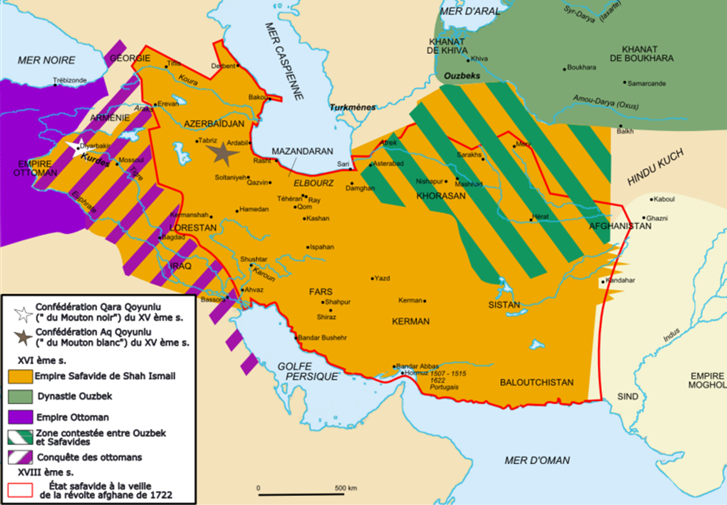
\includegraphics[width=\textwidth]{CourantsIslamContemporain/ImagesCourantsIslamContemporain/image2Chiisme.png}

     \label{fig:my_label}
 \end{figure}
 L'Iran était majoritairement sunnite jusqu'au Xème siècle. On a des populations turcophones à l'Ouest. un homme se proclame le Mahdi et fait la conquète militaire de l'Iran : par Isma'il en 1501.
  
 \paragraph{les limites du chiisme de Isma'il} conscient des limites du chiisme qu'il prone, il impose le chiisme duodécimain, venant du Liban, car le chiisme duodécimain était plus stable. Sans doute pour se détacher et légitimer face aux califes ottomans sunnites. Conversion de l'Iran assez violente : maudire les trois premiers califes, les confréries soufies. On va aussi déclarer les sunnites impurs.  


 
 %-------------------------------------------------
 
\section{Particularités de la doctrine chiite (duodécimaine ou imamite)
\label{particularituxe9s-de-la-doctrine-chiite-duoduxe9cimaine-ou-imamite}}


Elle s'est développée au VIII siècle par le 5ème et 6ème imams, qui étaient des savants. Ils ont collecté les corpus des hadiths, pas seulement du Prophète mais aussi des Imams, en particulier d'Ali et du 5ème et 6ème imams.

Ils ont développé l'école juridique
\begin{Def}[Ja'fariya]
 L'école juridique (madhhab) chiite dit Ja'fariya (aussi appelée école des Ahlul bayt) est la première école islamique apparue d'interprétation de fiqh du Coran d'inspiration chiite (contrairement aux quatre grandes écoles sunnites, avec lesquelles elle ne présente cependant pas de différences majeures).
\end{Def}
 %-------------------------------------------------
 
  \subsection{L'Imamat}
 La vraie spécificité du chiisme par rapport au sunnisme. 
 \begin{figure}[h!]
    \centering
        \sidecaption{lignée des imams}
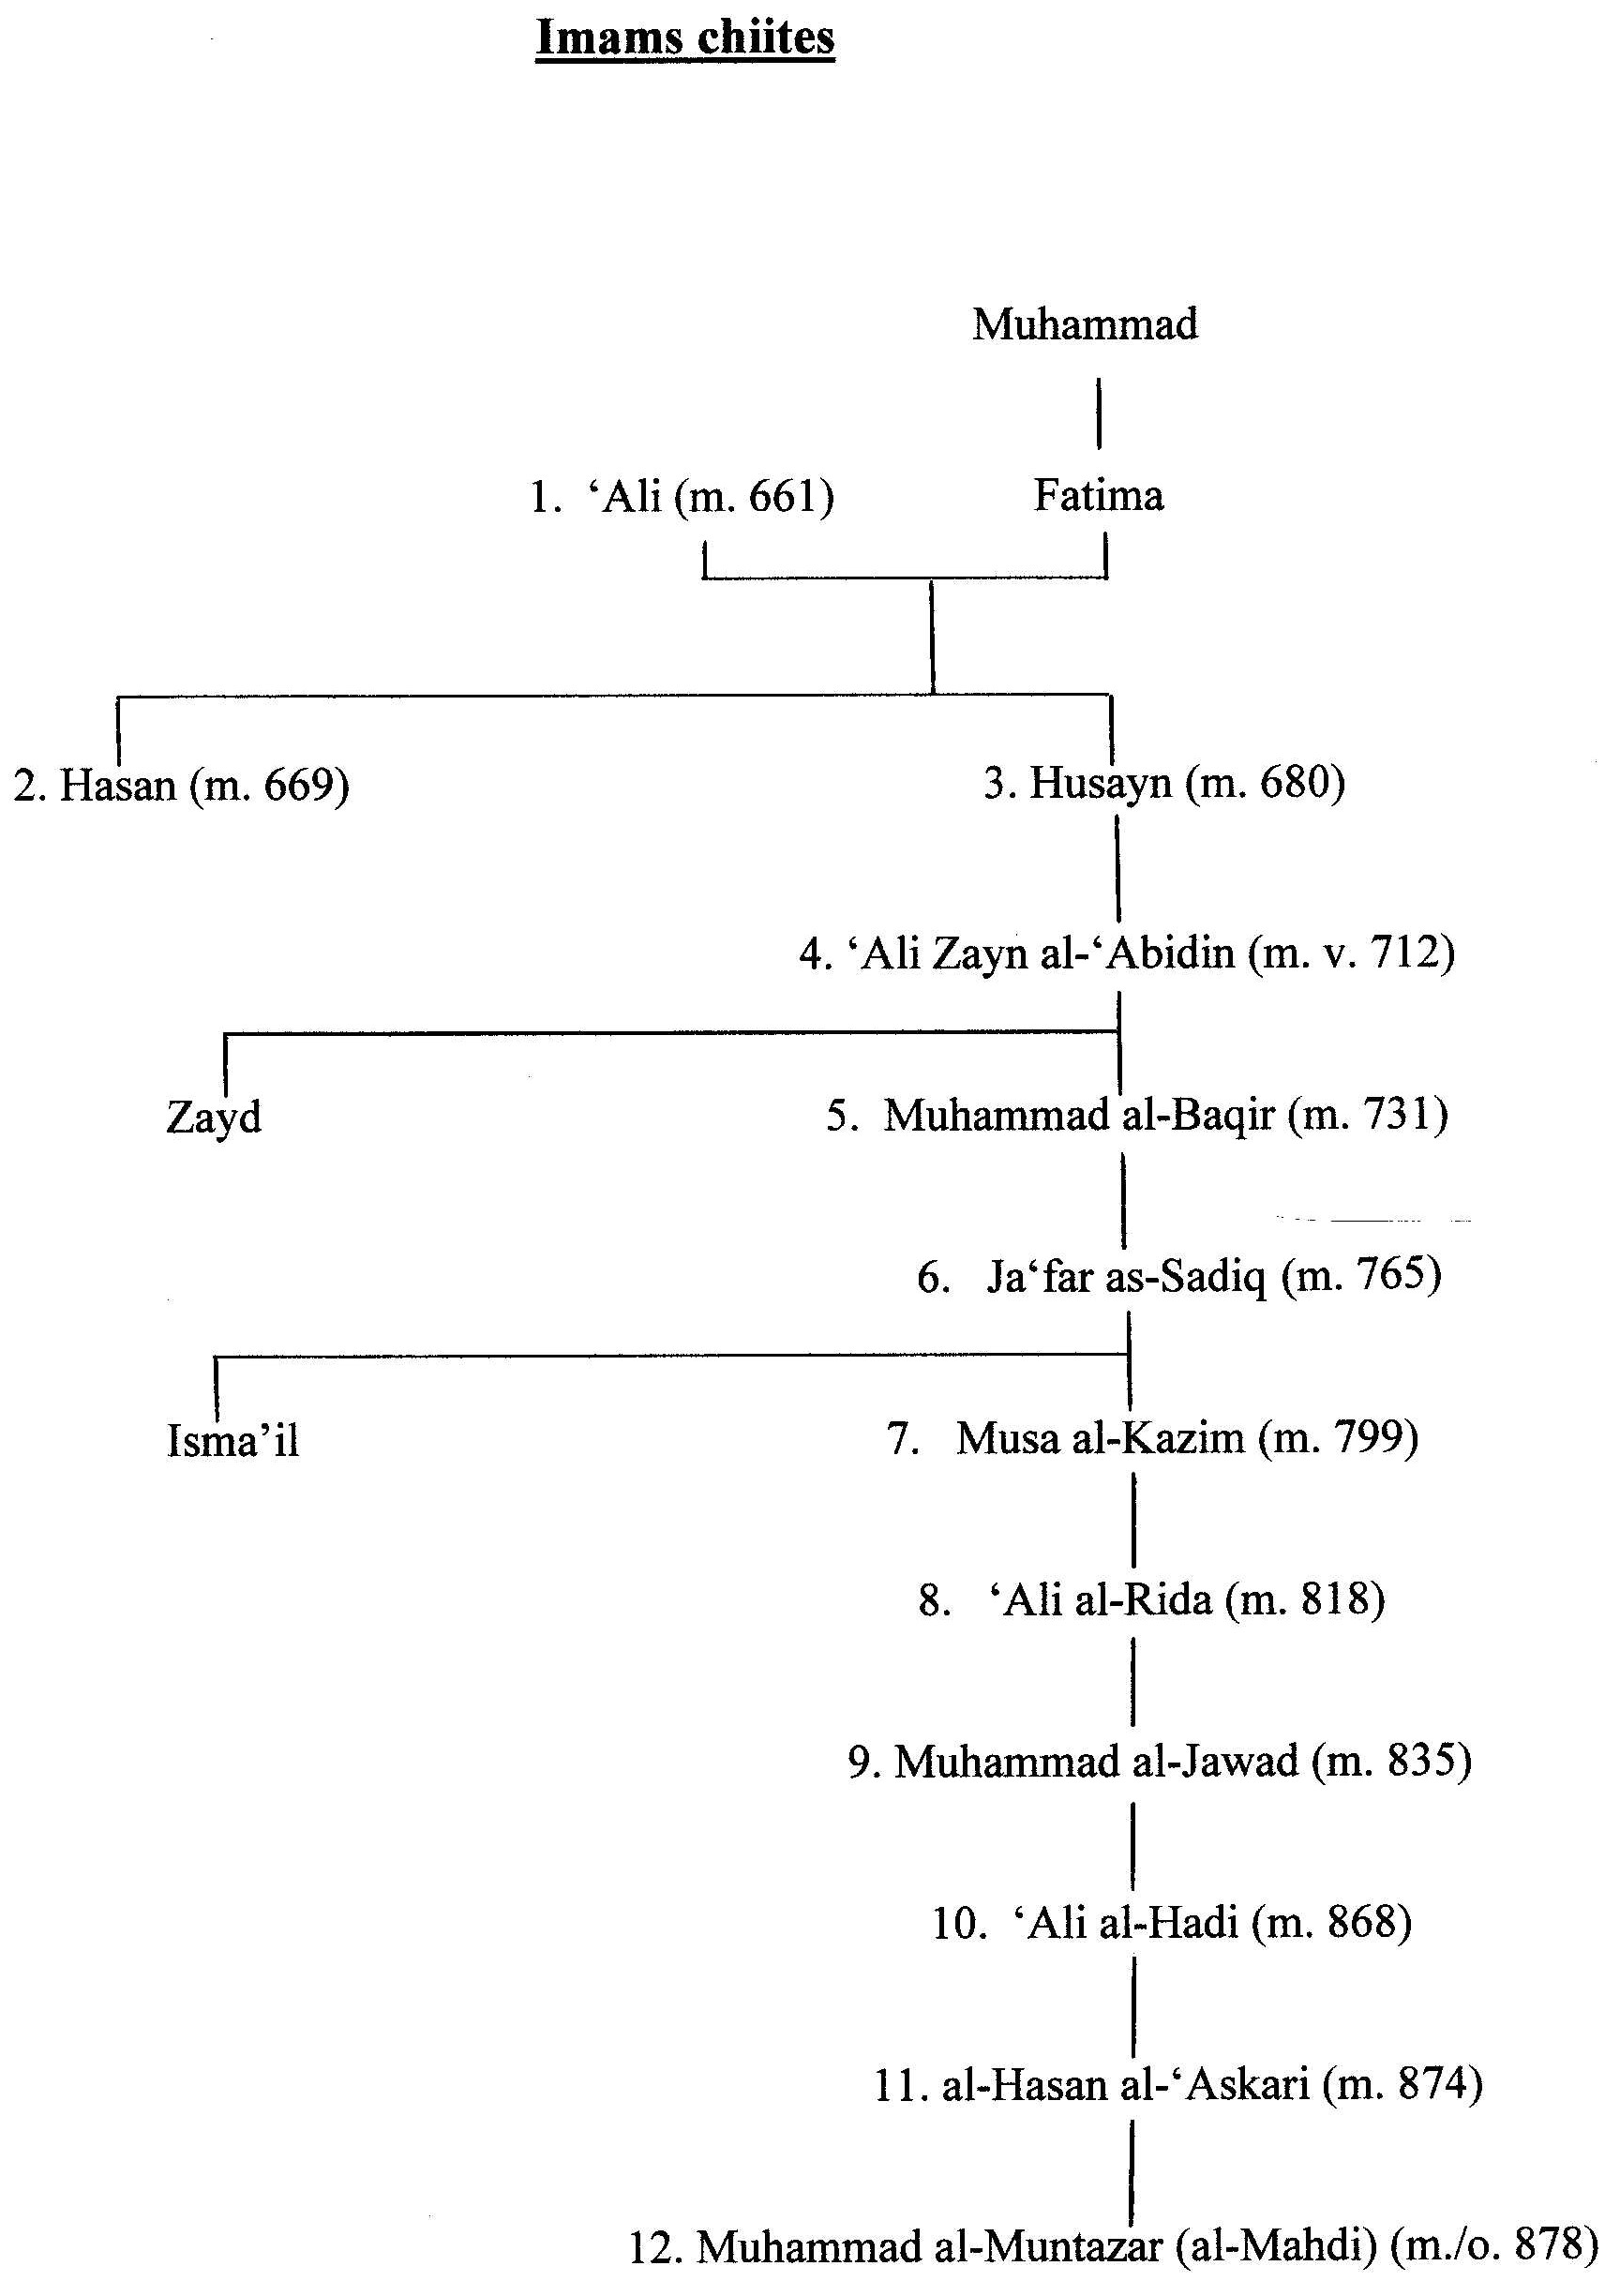
\includegraphics[width=0.8 \textwidth]{CourantsIslamContemporain/ImagesCourantsIslamContemporain/image2.png}
    \label{fig:my_label}
\end{figure}

 \paragraph{L'imam, celui qui guide} la prière et va faire le prêche du vendredi.  Dans la doctrine duodécimaine, l'imamat est lié à l'interprétation.
 Le prophète transmet la lettre du Texte. Mais elle a besoin d'être interprété : à chaque prophète dans l'humanité, correspond un imam : 
 \begin{itemize}
     \item Pour Moise, c'est Aaron
     \item Pour Jésus, c'est Pierre
     \item Pour Mohammad, c'est Ali.
 \end{itemize}
 Certes Mohammad est le dernier prophète, mais si on veut que le Coran soit parole vivante, il y a besoin d'Imams qui interprètent pour aujourd'hui la parole révélée.
 
 Du fait de problème de succession, il y a un vide à remplir (expliqué théologiquement par l'occultation), et c'est le \textit{clergé} qui le remplit \sn{Les Ayatollah ne sont pas imams. Il y a encore des imams dans le monde sunnite mais pas dans le monde chiite}.
 
 \newpage
 \paragraph{Les 14 immaculés}
    \begin{figure}
     \centering
     \sidecaption{Les 14 « Immaculés »  \newline La "Sainte Famille". \emph{Source}: Livre pour enfants iranien (Téhéran, 2006)}

\includegraphics[width=0.45\textwidth]{CourantsIslamContemporain/ImagesCourantsIslamContemporain/Image3Chiisme.jpeg}
\includegraphics[width=0.45\textwidth]{CourantsIslamContemporain/ImagesCourantsIslamContemporain/image4.jpeg}
 \end{figure}
 
 
 \begin{Def}[les 14 immaculés]
 Les Quatorze immaculés ou Les Quatorze Infaillibles (en arabe:\TArabe{ المعصومون الأربعة عشر)} est l'expression désignant les gens de la Sainte Famille du Prophète Muhammad (s) Ahl al-Bayt, qui sont au nombre de quatorze, le premier étant le Prophète lui-même, suivi de sa fille Fâtima Zahrâ (a) et des douze Imams (a) qui lui ont succédé.
 \end{Def}
 
 
  
  
  \subparagraph{Prophétie et imamat}
  
 
Une autre tradition savante rapporte :\sn{(Source : \emph{La religion discrète}, M-A Amir Moezzi, Paris, Vrin,
2006, p. 110)}
\begin{quote}
    

« Deux mille ans avant la création, Muhammad et Ali étaient une lumière
devant Dieu -- qu'Il soit glorifié et exalté -, lumière formée d'un
tronc principal d'où partait un rayon de lumière resplendissant\ldots{}
Dieu dit alors : « Voici une lumière {[}tirée{]} de Ma propre Lumière ;
son tronc est la prophétie et sa branche, l'imamat ; la prophétie
revient à Muhammad, Mon serviteur et messager, et l'imamat revient à
Ali, ma Preuve et mon Ami. Sans eux, je n'aurai rien créé de ma
création\ldots{} C'est pourquoi Ali répétait toujours : « Je proviens de
Muhammad {[}ou de Ahmad{]} comme une clarté provenant d'une
autre\ldots{} »
\end{quote}


 \paragraph{Une science divine} pour interpréter le Coran, il y a besoin d'une science divine. L'imam a reçu une dimension spirituelle, la \textit{lumière de l'imamat}. Les imams préexistait à la création du monde en tant que réalité spirituelle. Comme les prophètes, ils sont \textit{impeccables}, sans péché.
   \subparagraph{La divinité des Imams}
De nombreux hadiths des Imams soulignent leur caractère quasi-divin : \sn{Source : « Remarques sur la divinité de l'Imam », M-A Amir-Moezzi,
\emph{Studia Iranica}, n° 25, 1996, p. 193-216}


\begin{quote}


« Hommes ! Dieu créa Ses serviteurs afin que ceux-ci Le connaissent car
lorsqu'Ils le connaissent, ils L'adorent et se libèrent ainsi de
l'adoration de tout autre que Lui ». Un homme demande alors à l'imam : «
Qu'est-ce que la connaissance de Dieu ? » « C'est pour les gens de
chaque époque, la connaissance de l'imam {[}de cette époque{]} auquel
ils doivent obéissance » (Husayn ben `Ali)

« Dieu fit de nous Son œil parmi ses adorateurs, Sa Langue Parlante
parmi Ses créatures, Sa Main de bienveillance et de miséricorde étendue
au-dessus de Ses serviteurs, Sa face grâce à laquelle on se dirige vers
Lui, Son Seuil qui guide vers Lui, Son Trésor au ciel et sur la
terre\ldots C'est par notre acte d'adoration que Dieu est adoré, sans
nous, Dieu ne saurait être adoré » (Ja`far as-Sadiq)


\end{quote}
 \paragraph{Les 14 impeccables} Le prophète, les 12 imams et Fatima. \sn{pas de difficulté de représentations dans le chiisme, depuis les enluminures persanes jusqu'à aujourd'hui. }
 
 \paragraph{le sacrifice d'Hussayn}
 
{Le martyre de l'imam Husayn}

Dans ce contexte, le martyre de Husayn, 3\textsuperscript{ème} imam, est
interprété dans les termes d'un sacrifice cosmique \sn{Source : tradition orale relevée par A-S Vivier-Muresan : \emph{Afzâd.
Ethnologie d'un village d'Iran}, Peeters, 2006, p. 48.
}:

\begin{quote}
    
 
Avant que le monde ne soit, Dieu rassembla les âmes des Quatorze
Immaculés, déjà créées, en une grande assemblée et leur annonça que,
pour ce monde qu'Il était sur le point de façonner, « du sang doit être
donné, un nourrisson et un tout jeune marié tués, une jeune femme
emprisonnée ». Aucun n'eut la force d'accepter de telles souffrances, ni
même Muhammad, ni Ali, ni Hasan. Seul Hoseyn se porta volontaire. Dieu
insista :
 

\begin{itemize}
\item
 
  Tu devras donner les tiens.
  
\item
  
  J'accepte.
  
\item
 
  Tu devras donner ta tête.
  
\item
 
  J'accepte.
  
\item
  
  Une partie de ta famille devra connaître l'exil et la détention.
  
\item
 
  J'accepte.
  
\end{itemize}


Alors Gabriel lui donna à boire la coupe de la souffrance et lui fit
signer un pacte où étaient inscrites toutes ses promesses.

Bien plus tard, lors de sa vie terrestre, approcha le temps de son
sacrifice. Il se trouvait à Karbalâ, accompagné de 72 fidèles compagnons
et de toute sa famille, encerclé par les armées de Yazid. Une armée de
djinns vint alors proposer ses services mais Hoseyn refusa : le combat
aurait été trop inégal et il se rappelait par ailleurs sa promesse. La
lutte commença et de nombreux êtres chers à Hoseyn, compagnons, fils,
frères, cousins, tombèrent l'un après l'autre sous les coups de
l'ennemi. Aveuglé par la douleur, Hoseyn en oublia sa promesse, et se
mit à tailler en morceaux l'armée adverse. Dieu s'empressa alors
d'envoyer Gabriel lui tendre le pacte qu'il avait signé au début des
temps. Rappelé à la raison, Hoseyn se soumit à la volonté divine et tint
son serment ; il retira son épée du combat et se livra à la fureur de
ses adversaires qui ne tardèrent pas à le mettre en pièces.
\end{quote}

 \subparagraph{Kerbala} la mémoire de la bataille est aussi une fête populaire. Des maquettes, repas,... le rouge reflète les partisans d'Hussayn.
 
 \begin{Def}[ta'ziyya]
\emph{représentation théâtrale du drame de Kerbala}
 \end{Def}

\begin{figure}[h!]
    \centering
        \sidecaption{Karbala}
    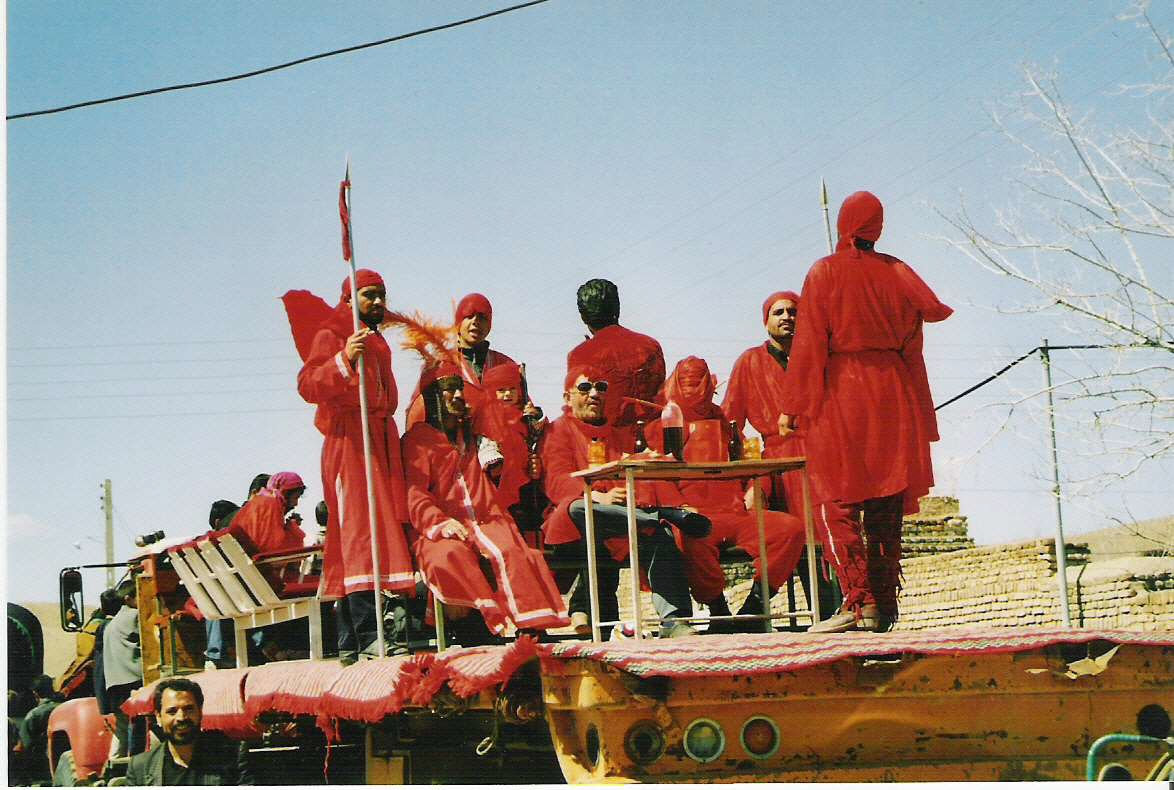
\includegraphics[width=0.3\textwidth]{CourantsIslamContemporain/ImagesCourantsIslamContemporain/image9.jpeg}
    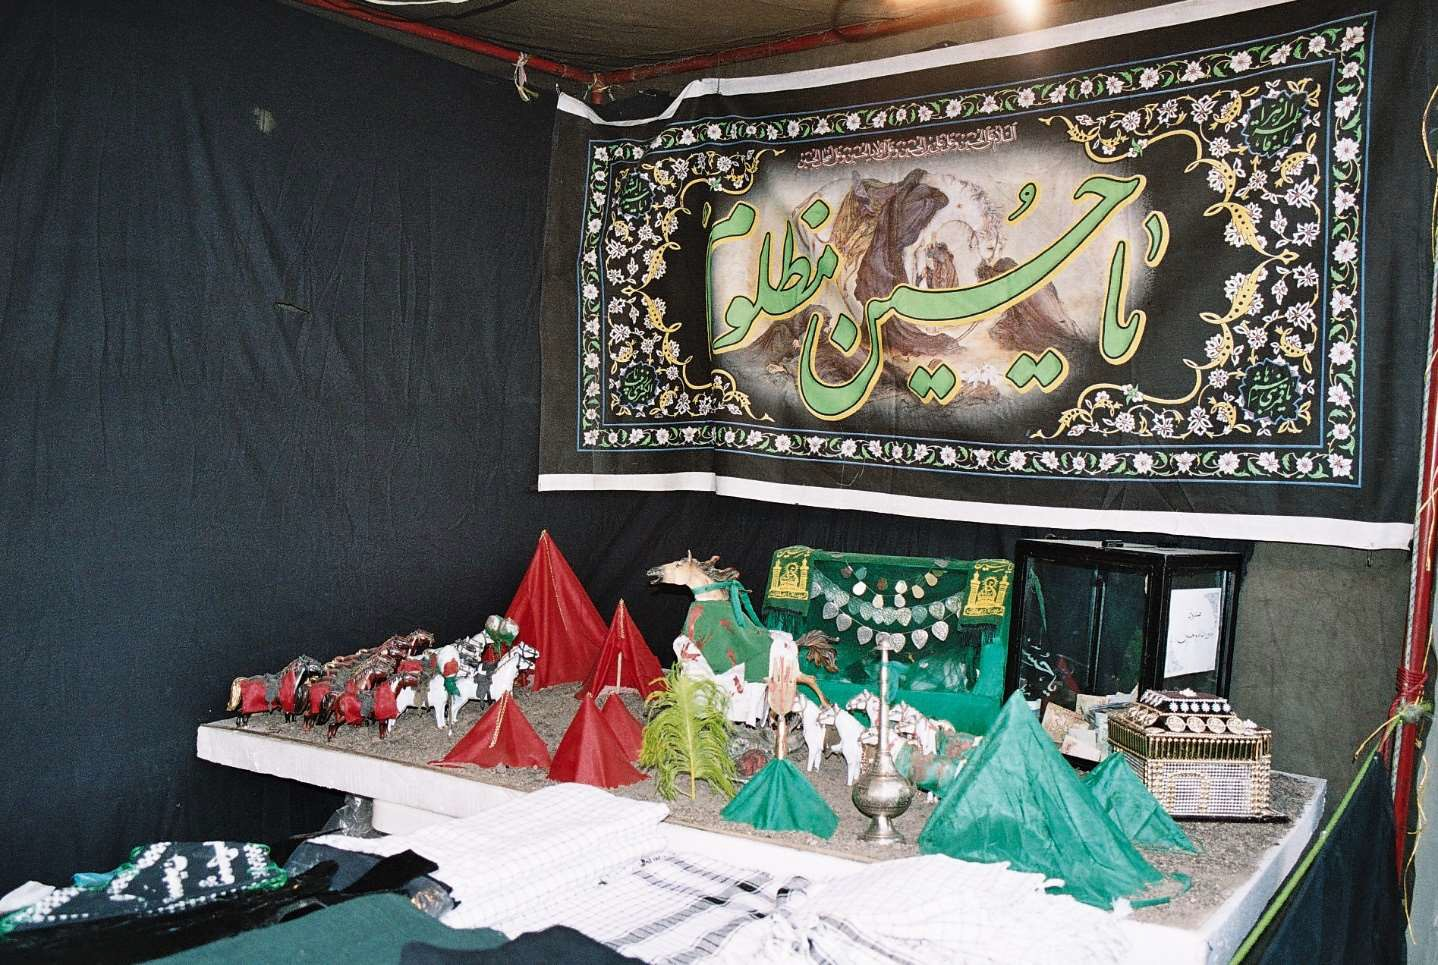
\includegraphics[width=0.3\textwidth]{CourantsIslamContemporain/ImagesCourantsIslamContemporain/image10Chiisme.jpeg}
        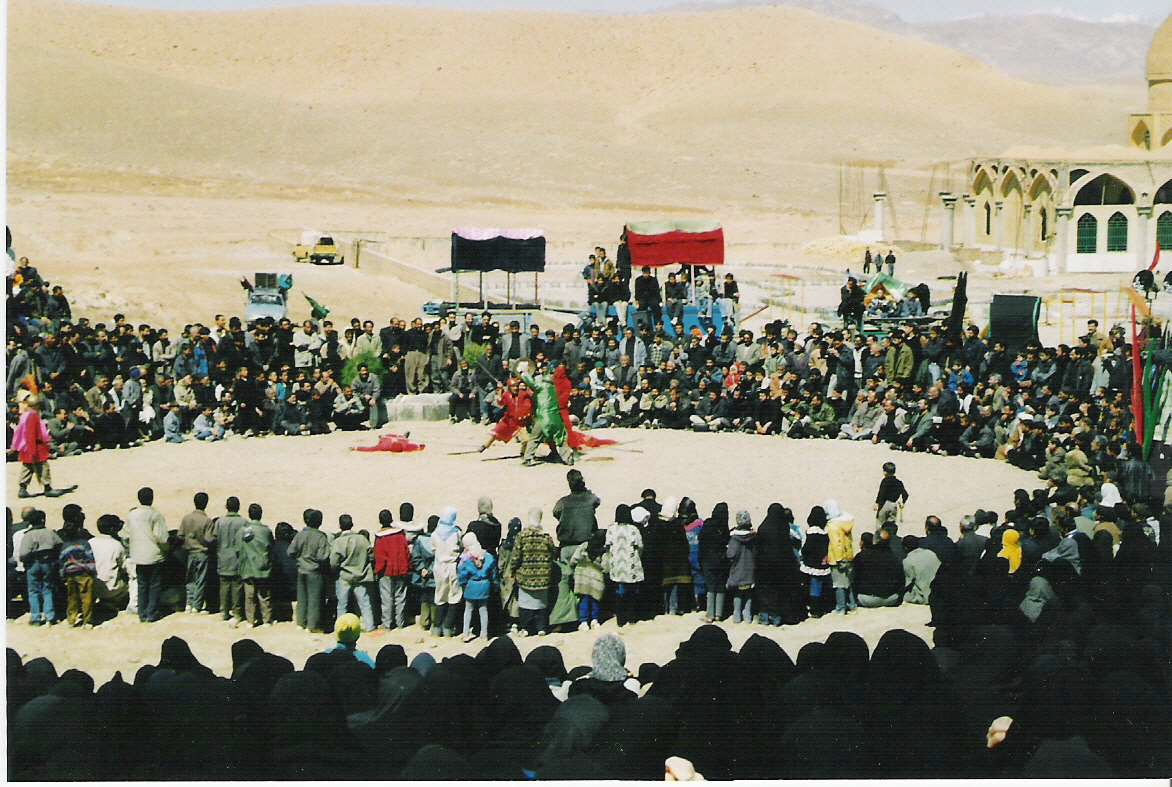
\includegraphics[width=0.3\textwidth]{CourantsIslamContemporain/ImagesCourantsIslamContemporain/image8.jpeg}


    \label{fig:my_label}
\end{figure}
 
 
 %-------------------------------------------------
 
  \subsection{Le corpus coranique et son interprétation}
 
 
  \paragraph{Le « Coran chiite »}
 
 Le Coran actuel aurait été purgé des 2/3, en particulier par tout ce qui touche 'Ali.


\begin{quote}
Certains écrits chiites rapportent des citations du «Coran intégral»
qui aurait été par la suite altéré par les sunnites. Ces citations
présentent des divergences parfois notables avec la recension
officielle, comportant souvent des mots, expressions ou bouts de phrase
absents de celle-ci (en italique dans le texte).

C. 4, 167-70 : « Ceux qui sont injustes \emph{à l'égard des droits de la
Famille de Muhammad}, Dieu ne les pardonnera ni ne les guidera sur aucun
chemin si ce n'est sur celui de la géhenne où ils y séjourneront à
jamais et c'est chose facile à Dieu.

C. 16, 24 : « Et quand on leur dit : `\,`Qu'a fait descendre votre
Seigneur \emph{au sujet de `Ali} ?'\,' Ils répondent : `\,`Fables
racontées par les Anciens'\,' » ?

C. 33, 71 : « Quiconque obéit à Dieu et à Son prophète \emph{en ce qui
concerne la walaya de `Ali et la walaya des imams après lui}, celui-là
jouit d'un bonheur grandiose ».

C. 42, 13 : « Il a établi pour vous, \emph{ô famille de Muhammad}, en
fait de religion, ce qu'Il avait prescrit à Noé, et ce que Nous te
révélons \emph{ô Muhammad}, et ce que Nous avons prescrit à Abraham, à
Moïse et à Jésus : `\,`Etablissez la religion \emph{de la famille de
Muhammad}, ne vous divisez pas à son sujet et soyez unis ».

(Source : \emph{La religion discrète}, M.A Amir-Moezzi, Paris, Vrin,
2006, p. 179-180)
\end{quote}
 
 A la fin du XIX, cette posture chiite a été abandonnée car le réformiste chiite a essayé de se rapprocher du sunnisme. De façon générale, le Coran lu en Iran a toujours été le même mais avec une suspiçion qu'il ne contenait pas tout.
 

 %-------------------------------------------------
 
  \subsection{Le rôle des clercs}
  
  \paragraph{Un sens caché du Coran, ésotérique} Seul l'imam peut interprété le Coran. \textit{"si le grand ayatolah nous dit qu'on ne doit plus prier 5 fois par jour, on le suit".} \sn{L'absence de médiation dans le sunnisme est à relativiser quand on voit l'importance pour les sunnites de ce qui est Halah et Haram et qui demandent à l'imam...}
 
 \paragraph{Les clercs vont se substituer à l'Imam} pour l'interprétation du Coran et du droit. 
 
 \paragraph{Direction de la prière} A l'époque safavide, le clerc est nécessaire pour diriger la prière. On ne peut prier collectivement sans clerc. Le clerc va s'occuper des taxes religieuses.
 \paragraph{Au XIX, déclaration du Jihaad} Alors que c'est normalement l'Imam.
 
 \paragraph{Une dernière étape, avec l'Ayatollah Khomeini, le pouvoir politique} Toutes les prérogatives normalement réservées à l'Imam.
 
 \paragraph{Un clergé très structuré}. 
 \begin{itemize}
     \item les \emph{marja} (taqlid), la \emph{source} (de l'imitation). Un fidèle doit imiter un marja. Une dizaine dans le monde. Ils se cooptent (des dynasties de Marja et d'ayyatollah). Khomeini était \textit{marja}.
     \item l'\emph{ayyatollah} qui est le seul à interpréter le Coran, une centaine dans le monde, dont quelques femmes
     \item le \emph{hojjatelislam} qui a l'équivalent d'un doctorat
     \item le \emph{mollah}, \emph{âkhund} qui dirige la prière
 \end{itemize}
 
 
 %-------------------------------------------------
 
  \section{D'autres courants chiites :
  Zaydites et
  Ismaéliens} 
 
   \subsection{Le zaydisme}
   
   Proche du sunnisme, ils reconnaissent même les trois premiers califes, ce qui est inconcevable dans le chiisme duodécimain (cf la cérémonie de bruler Omar de Khomeini).
   Environ 1 million de fidèle.
   
   \subsection{Le chiisme septimain (ismaélisme)}
   A l'autre extrême, l'imam est quasiment une incarnation de Dieu. Un primat de l'ésoterisme, occulte. Un grand rôle donné à l'initiation. Un certain recul par rapport aux pratiques, à relativiser. 

\paragraph{L'Aga Khan} chef spirituel des septimains.
 



 
\section{Glossaire}
 
\subsection{Personnes} Abbas Abu Bakr

Adud ad-Dawla Al-Karaki Hasan as-Sabah Isma'il

Kulayni (\emph{Kitab al-Kafi}) Mu'awiya (omeyyades) Nizar

Omar Osman Quraysh Yazid

{Lieux} Alamut Ardabil

Ghadir al-Khumm Jabal al-Amil Kerbala

Khorasan Kufa Machhad Sham Siffin

{Autres noms propres} akhbari

ja`farisme (école juridique chiite) kharijites

Mamlouks

Muharram (mois musulman) mu`tazilites

nizayri Qarmates Seljukides usuli

\subsection{Notions}



baten : \emph{ésotérique} (c. zaher) faqih (pl. fuqaha) : \emph{juriste}

fitna: \emph{discorde, querelle (conflit interne au monde musulman)}

ghulat : \emph{groupes chiites aux doctrines}

\emph{« extrémistes »}

hulul : \emph{« incarnation »}

ijtihad : \emph{effort personnel d'interprétation (des textes sacrés)}

`ilm : \emph{science}

imamzade : \emph{descendant des Imams / sanctuaire contenant leur
tombeau} (persan)

`isma : \emph{impeccabilité}



ma`sum : \emph{impeccable (sans péché)} mujtahid : \emph{celui qui
pratique l'ijtihad} najes : \emph{impur} (persan)

na'ib : \emph{délégué}

na'ib al-`amm : \emph{représentant général de l'Imam}

nass : \emph{élection divine}

tafsir : \emph{commentaire (exotérique) du Coran}

tanasukh : \emph{métempsychose}

ta'wil : \emph{herméneutique ésotérique du Coran} 


taqiyya : \emph{dissimulation (fait de cacher sa foi)} walayat al-faqih
(persan : velayat-e faqih) : \emph{gouvernement du juriste}

zaher : \emph{exotérique} (c. de baten)
 
 


 



 


 


\hypertarget{sabrina-mervin}{%
\section{Annexe : Les Autorités religieuses dans le chiisme duodécimain
contemporain - Sabrina Mervin}\label{sabrina-mervin}}

 \mn{
Référence électronique

Sabrina Mervin, « Les Autorités religieuses dans le chiisme duodécimain
contemporain », \emph{Archives de sciences sociales des religions} {[}En
ligne{]}, 125 \textbar{} janvier - mars 2004, mis en ligne le 22 février
2007, consulté le 17 octobre 2012. URL :
\url{http://assr.revues.org/1033} ; DOI : 10.4000/assr.1033

Éditeur : Éditions de l'École des hautes études en sciences sociales
\href{http://assr.revues.org/}{http://assr.revues.org}

\href{http://www.revues.org/}{http://www.revues.org}

}



 

En 1890, pour renflouer les caisses de l'État iranien, Nâsir al-Dîn Shah
accorda au baron de Reuter, sujet britannique, une concession qui lui
garantissait pour cinquante ans le monopole de la culture, de la vente
et de l'exportation du tabac. Aux yeux des Iraniens, c'était brader les
ressources du pays à des étrangers. La colère gronda, autant dans les
cercles cléricaux que dans les milieux bazaris et parmi la population.
Le Shah refusa d'entendre les injonctions des oulémas comme de plier
devant les manifestations populaires. L'activiste réformiste Jamâl
al-Dîn al-Asadâbâdî al-Afghânî (1), qui venait d'être exilé par le
souverain, poussa le grand chef religieux chiite de l'époque, un Persan
qui résidait à Sâmarrâ', Muhammad Hasan al-Shîrâzî, à réagir. En
décembre 1891, celui-ci promulgua une \emph{fatwâ} déclarant la
consommation de tabac illicite. Le boycott fut suivi dans tout le pays,
jusqu'au sein même de la cour du Shah, qui dut finalement plier et
annuler la fameuse concession (2).

Si le fait constitue un événement historique, traité en tant que tel par
les histo- riens de l'Iran, il est rapporté de façon récurrente par les
oulémas chiites, comme un récit exemplaire. Il leur sert à édifier les
croyants non seulement sur l'efficacité du boycott, c'est-à-dire de la
solidarité nationale, face aux compagnies étrangères, mais aussi sur
leur propre rôle dans la société, leur rapport au pouvoir, et l'étendue
de leur autorité. Ainsi, par exemple, le clerc libanais Muhsin al-Amîn
la raconta à ses amis nationalistes, à Damas, pour les encourager à
boycotter la Régie de l'élec- tricité, détenue par des intérêts
français, dans la Syrie sous mandat des années 1930. « Le Shah lui-même
ne pouvait plus fumer de narguilé, car les femmes du palais les avaient
tous fait disparaître, pour obéir à la \emph{fatwâ} d'al-Shîrâzî... »,
leur expliqua-t-il (3). Voilà pour démontrer l'efficacité de la
solidarité nationale. Quant à l'autorité des clercs, elle est corroborée
par l'anecdote suivante qui complète le récit du boycott du tabac et
circule encore, de nos jours, dans les milieux cléricaux
chiites, par écrit ou oralement. Le directeur de la compagnie
britannique voulut s'enquérir sur celui qui entravait son projet, afin
de mieux le combattre. Il demanda : « De combien d'hommes dispose-t-il ?
». On lui répondit que le clerc n'avait pas d'armée. « À combien se
monte sa fortune ? », poursuivit-il. On lui dit qu'il n'avait pas de
fortune et vivait très simplement. Le Britannique rétorqua alors que,
dans ces conditions, rien ne pouvait être tenté contre cet homme.

C'est non sans fierté que les chiites rapportent cette anecdote. Toute
l'autorité de leurs oulémas réside là : d'un mot, ils peuvent braver le
pouvoir en place, alors que le pouvoir n'a aucune prise sur eux,
puisqu'ils n'ont pas véritablement d'ambi- tion mondaine. On pense à
Khomeini défiant le Shah. Avec lui, l'autorité des clercs fut poussée à
son paroxysme, avec les conséquences que l'on sait, à savoir l'instau-
ration de la République islamique d'Iran. Certes, la figure du clerc
contestataire qui défie le pouvoir n'est pas propre au chiisme,
l'histoire de l'islam sunnite en fournit assez d'exemples, d'Ibn
Taymiyya (m. 1328) à Abd al-Salâm Yâsîn. Le premier s'en prit aux
Mongols, des envahisseurs qui s'étaient emparés du pouvoir et dont il
jugeait l'adhésion à l'islam superficielle. En outre, il blâma aussi les
soufis qui, au sein de sa propre société, s'adonnaient à des pratiques
rituelles non conformes à l'islam rigoriste qu'il prônait (4). Le second
est un cheikh marocain contemporain qui osa s'en prendre au roi Hasan II
en lui adressant un « conseil » (\emph{nasîha}). Il s'ancrait ainsi à la
fois dans la tradition islamique, qui permet au clerc d'admo- nester le
prince, grâce au principe affirmant la nécessité de commander le bien et
d'interdire le mal, et dans une tradition locale de clercs
contestataires, connue de son public. Son autorité sur les croyants fut
renforcée par le statut d'opposant poli- tique qu'il acquit suite à ce
défi, puisqu'il fut astreint à résidence surveillée (5).

Les oulémas chiites n'ont donc pas le monopole de la contestation.
Toutefois, on s'accorde à dire que, en général, les oulémas sunnites ont
eu tendance, au cours de l'histoire, à légitimer les pouvoirs en place,
alors que les chiites ont plutôt adopté une attitude de réserve à leur
égard. Au-delà des similitudes évidentes entre les oulémas des deux
grandes branches de l'islam, il importe de souligner que les chiites ont
des particularismes, autant dans le fondement de leur autorité que dans
les modalités de son fonctionnement. Pour résumer et schématiser les
processus en œuvre, on peut dire que l'autorité des oulémas sunnites,
depuis la centralisation imposée par l'Empire ottoman, l'application des
\emph{tanzîmât} et le contrôle du champ religieux instauré par les États
modernes, tend à se réduire. Alors que c'est l'inverse chez les oulémas
chiites, qui ont conquis leur pouvoir religieux et assis leur autorité
au fil des siècles et, surtout, depuis la seconde moitié du
XIX\textsuperscript{e} siècle. On va voir comment l'épisode de la
\emph{fatwâ} de Shirazi s'insère dans ce mouvement.

Selon la doctrine chiite, les douze imams infaillibles détenaient, de
leur vivant, toute forme d'autorité. En effet, les exégètes chiites
interprètent différemment des sunnites le verset coranique : « Ô vous
qui croyez ! Obéissez à Dieu et obéissez au Prophète et à ceux d'entre
vous qui détiennent l'autorité » (IV, 59). Pour les sunnites, les
détenteurs de l'autorité (\emph{ûlû al-amr}) peuvent être les califes et
les rois ; pour les chiites, ce sont les imams (6). À l'instar du
prophète Muhammad, dont ils transmirent la \emph{sunna}, les imams
étaient, pour leurs fidèles, les guides de la
communauté et les détenteurs des pouvoirs spirituel et temporel (7).
C'est pourquoi les califes et les rois qui lui succédèrent furent
considérés par les chiites comme des chefs injustes ou des oppresseurs.
En outre, dans les doctrines chiites, l'imamat fait partie des
fondements de la religion et complète la prophétie. Comme le prophète et
sa fille Fâtima, les imams sont tenus pour infaillibles : ils ne commet-
tent pas d'erreur. Par ailleurs, selon les anciens \emph{hadîth}
chiites, seuls les imams sont habilités à décliner les normes de la loi
sacrée.

Or, selon les doctrines, le douzième imam « disparut », entra en
occultation, en 874. Vivant, mais caché, il continua, dans un premier
temps, à communiquer ses prescriptions aux fidèles par l'intermédiaire
de quatre agents : ce fut la période de l'occultation mineure. Puis, à
partir de 941, il cessa d'avoir recours à des agents, et le lien avec
ses adeptes fut rompu : on entra dans la période de l'occultation
majeure, qui se poursuit actuellement. Les croyances chiites veulent
que, au terme de cette période, l'imam attendu, le Mahdî ou Qâ'im,
reviendra sur terre pour y restaurer la justice, avant la fin des temps
et le jugement dernier.

Ainsi, à partir de 941, la communauté des croyants se retrouva sans
guide, aussi bien pour les affaires spirituelles que pour les affaires
temporelles. Selon le \emph{hadîth} chiite, « Toute bannière élevée
avant le soulèvement du Qâ'im appartient à un rebelle contre Dieu
(\emph{tâghût)} », tout pouvoir politique était considéré comme inique,
illégitime (8). Or, le temps passant, il devenait de plus en plus
difficile, pour la communauté, de se passer d'autorité, de référence.
Des questions centrales restaient sans réponse : à qui verser les impôts
religieux ? Qui peut diriger la prière du vendredi ou lancer le
\emph{jihâd} ? Qui détient le pouvoir de statuer, de juger, d'arbi- trer
les conflits et de faire appliquer les peines, en l'absence de l'imam ?
Peu à peu, les oulémas procédèrent à une élaboration doctrinale, afin de
s'attribuer les fonc- tions et les pouvoirs de l'imam, et d'agir en son
nom en tant que son délégué (\emph{nâ'ib al-imâm}) (9). En outre, ils
impulsèrent un processus de rationalisation, voire d'idéologisation des
doctrines qui s'effectua par étapes successives, au moyen, notamment, de
l'introduction de différents concepts clefs. C'est ce long processus qui
allait permettre à Khomeini de concevoir sa théorie de \emph{wilâyat
al-faqîh}, « le pouvoir politico-charismatique » ou « guidance » du
théologien-juriste, sur laquelle est fondé l'État islamique en Iran
(10).

L'ouverture de la « porte de l'\emph{ijtihâd} », selon l'expression en
vigueur, est le volet principal de ce processus. L'exercice de
l'\emph{ijtihâd} consiste à extraire les pres- criptions du droit
islamique des quatre sources de ce droit, c'est-à-dire, d'une part, des
textes sacrés que sont le Coran et la \emph{sunna} et, d'autre part,
d'une série de méthodes et de techniques que l'on regroupe autour des
concepts de consensus (\emph{ijmâ`)} et de raisonnement analogique
(\emph{qiyâs}) chez les sunnites, et de raison (\emph{`aql}) chez les
chiites. C'est dire qu'il s'agit d'élaborer les normes de la loi sacrée,
la \emph{charî`a}. Le fait d'exercer l'\emph{ijtihâd} permet donc de
répondre à de nouvelles ques- tions, de réagir à de nouvelles situations
et, plus largement, d'introduire le changement dans les normes tout en
revenant aux textes. Il s'oppose au \emph{taqlîd}, le conformisme
juridique, consistant à reproduire les normes établies par les anciens.

C'est dans ce mouvement d'ouverture que réside une différence
essentielle entre l'histoire des doctrines chiites et celle des
doctrines sunnites. En effet, même si cette théorie doit être modulée et
affinée aujourd'hui, les historiens admettent que le droit islamique
sunnite est théoriquement figé, depuis la fixation de ses quatre écoles
(malékite, hanéfite, hanbalite et chaféite), au XI\textsuperscript{e}
siècle. Depuis cette date en effet, les juristes ont eu une large
tendance au conformisme, hormis les exceptions notoires de grands
savants de l'islam tels Ghazâlî (m. 1111), Ibn Taymiyya (m. 1328) ou
Suyûtî (m. 1505). Cette situation a perduré jusqu'au
XVIII\textsuperscript{e} siècle, lorsque quelques oulémas commencèrent à
prôner l'exercice de l'\emph{ijtihâd}. Puis, le mouvement s'est
intensifié, à partir de la fin du XIX\textsuperscript{e} siècle, quand
des modernistes revendiquèrent la réouverture de sa porte, afin de
mettre l'islam en accord avec l'esprit du siècle. On considère ainsi que
c'est le choc avec la culture envahissante de l'Europe qui incita des
oulémas réformistes à réagir et à entamer une réflexion sur la question.

Les doctrines chiites connurent le mouvement inverse. Alors que la porte
de l'\emph{ijtihâd} se fermait chez les sunnites, les chiites
s'employèrent à l'ouvrir de plus en plus largement et à octroyer des
pouvoirs croissants aux oulémas. Al-Tûsî (m. 1067) donna la première
impulsion à ce mouvement, que poursuivirent les savants de Hilla Ibn
Idrîs (m. 1201), al-Muhaqqiq (m. 1277), al-`Allâma (m. 1325), puis
d'autres du Jabal `Âmil (l'actuel Liban-Sud), Zayn al-Dîn al-`Âmilî dit
« le Second Martyr » (m. 1557) et son fils Hasan (m. 1602). Au même
moment, en Iran, le souverain safavide Shah Tahsmap nommait le juriste
al-Muhaqqiq al-Karakî (m. 1534) représentant de l'imâm (11). Ce courant
du chiisme duodécimain, appelé \emph{usûlî}, se renforça au
XIII\textsuperscript{e} siècle ; il devint majoritaire, et les doctrines
s'affinè- rent (12).

\hypertarget{linstitution-de-la-marjaiyya-pilier-de-lautorituxe9-religieuse}{%
\subsection{L'institution de la marja`iyya, pilier de l'autorité
religieuse}\label{linstitution-de-la-marjaiyya-pilier-de-lautorituxe9-religieuse}}

Un pas décisif fut franchi avec la systématisation de la référence à un
savant habilité à exercer l'\emph{ijtihâd}, en matière de prescriptions
religieuses. Elle fut mise en œuvre par Murtadâ al-Ansârî (m. 1864), qui
institua la fonction de \emph{marja`,} « réfé- rence à suivre », ou «
source d'imitation » pour les croyants (13). Selon cette théorie, les
croyants doivent se conformer aux avis émis par le \emph{marja`}, pour
tout ce qui concerne les questions afférant au droit islamique : d'où un
nouveau sens du terme \emph{taqlîd}, qui désigne désormais, pour les
chiites, le fait de se conformer aux prescriptions d'un \emph{marja`}
vivant, et non pas, comme c'est le cas chez les sunnites, de se
conformer aux écrits des anciens oulémas d'une école juridique donnée.
Les prescriptions, parallèlement, s'étaient élargies à tous les domaines
de la vie sociale et politique. Ainsi les oulémas pouvaient-ils
s'arroger certaines fonctions de l'imam, comme celle de déclarer le
\emph{jihâd} : ce que fit Ja`far Kâshif al-Ghitâ' (m. 1812), lorsqu'il
autorisa Fath `Alî Shah à mener la guerre sainte contre les
Russes (14). Si, par ce geste, le clerc cautionna la politique du
prince, d'autres cessèrent ensuite de composer avec le pouvoir, quitte à
s'opposer à lui. La \emph{fatwâ} que promulgua Muhammad Hasan al-Shîrâzî
fut une première étape. Après cela, des clercs s'investirent dans les
affaires politiques et, notamment, participèrent au mouvement
constitutionnaliste (1906-1911) visant à restreindre le pouvoir du Shah.

Après les travaux d'al-Ansârî, d'autres oulémas précisèrent la doctrine,
quant aux modalités du \emph{taqlîd} et aux critères de choix du
\emph{marja`}, et mirent en place le fonctionnement de l'institution.
Plus tard, des écrits tendirent à montrer qu'elle datait des débuts du
chiisme et dressèrent des listes de \emph{marja`}, à partir des plus
anciens. Même si l'idée a été reprise par des chercheurs, il s'agit bien
là d'une
« tradition inventée » (15).

Selon cette doctrine, tout croyant doit suivre les prescriptions d'un
\emph{marja`}, énoncées par celui-ci dans un traité pratique de droit
islamique, ainsi qu'à ses \emph{fatwâ.} S'il opte pour un \emph{marja`}
selon des règles établies, elles ne sont pas contrai- gnantes et son
choix s'opère donc, au bout du compte, en toute liberté. Les ancrages
ethniques, claniques, locaux et familiaux constituent bien évidemment
des facteurs influents, mais pas forcément décisifs. En outre, il arrive
que des adeptes d'un \emph{marja`} en suivent un autre, pour certaines
questions : ainsi, par exemple, dans les années 1980, bon nombre de
chiites suivaient Kho'i (m. 1992) pour les ques- tions religieuses
classiques, et Khomeini (m. 1989) pour les affaires politiques. Kho'i
étant par ailleurs très rigoriste en matière de voile, puisqu'il
prescrivait aux femmes de se cacher le visage, il leur laissait le
loisir de suivre un autre \emph{marja`,} sur ce point précis ; certaines
se référaient donc à Khomeini en la matière (16). Enfin, le croyant doit
régler ses impôts religieux au \emph{marja`} qu'il suit. Ainsi, il lui
verse la \emph{zakât}, un impôt commun aux grandes branches de l'islam,
mais aussi le \emph{khums}, spécifique au chiisme, se montant au
cinquième de ce qui lui reste lorsqu'il a dépensé ce qu'il lui faut pour
vivre.

Avec l'instauration du système de \emph{taqlîd}, un lien direct est donc
établi entre le croyant et un clerc de haut rang auquel il se réfère
pour suivre les préceptes de la loi, et ainsi assurer son salut. C'est
l'une des raisons pour lesquelles on parle parfois de « clergé »
concernant les autorités religieuses chiites qui, en outre, sont
organisées en une manière de hiérarchie. Toutefois, celle-ci est très
différente de la hiérarchie chrétienne, à laquelle on la compare
parfois, et même du système sunnite mis en place par les Ottomans, dont
se sont inspirés les États musulmans modernes.

Il n'y a aucune procédure de désignation formelle du \emph{marja`} ;
celui-ci n'est ni élu, ni désigné : on dit qu'il « émerge ». En fait,
tout se joue à trois niveaux : celui des cercles des clercs de haut
rang, celui des milieux commerçants et financiers influents, et,
\emph{in fine}, au niveau des croyants qui entérinent, ou non, les avis
des précédents. Ajoutons à cela l'influence éventuelle de l'État, sur
laquelle nous reviendrons. Le \emph{marja`} doit, d'abord, être reconnu
comme le plus savant de son temps et jouir d'une grande réputation dans
l'enseignement des sciences reli- gieuses ; c'est le premier critère de
sélection. Ensuite, il doit faire preuve de piété et de probité morale,
et être capable de percevoir les impôts et de les employer à subvenir
aux besoins des étudiants en sciences religieuses. Voilà donc les
principales qualités requises pour prétendre à la fonction, qui
s'ajoutent aux critères de bases, à savoir : être un homme, de naissance
légitime, d'âge mûr, et doué d'intelligence.

La première condition à remplir pour devenir \emph{marja`,} être « le
plus savant » en sciences religieuses, est difficile à apprécier. Aussi,
des critères plus ou moins objectifs ont été peu à peu mis en œuvre.
Avant tout, il faut compter parmi les oulémas de haut niveau, dûment
habilités à exercer l'\emph{ijtihâd} par leurs maîtres, et donc
détenteurs de certificats l'attestant. Dans les cercles de ces savants,
appelés \emph{mujtahid}, il faut être reconnu comme l'un des meilleurs.
Ce qui ne peut advenir à un jeune clerc, mais requiert âge et
expérience. En outre, la réputation du candidat se « mesure » au nombre
des étudiants qui suivent son enseignement, et à la manière dont ils le
reçoivent : s'ils prennent le soin de noter précisément les cours du
maître, et de les publier, cela ne lui donne que plus de poids. C'est
donc au sein de l'école en sciences religieuses, la \emph{hawza}, et
dans les cercles de ses pairs que le \emph{mujtahid} commence à se
distinguer. S'il répond aux incitations de son entourage à rédiger un
traité pratique de droit islamique, susceptible de devenir un guide pour
les croyants, il se pose alors en candidat à la \emph{marja`iyya}. Des
hommes d'influence (religieuse, sociale, financière) interviennent pour
le promouvoir et, au bout de la chaîne, les fidèles vont décider de se
référer à lui, ou non : l'allégeance populaire est la dernière étape.
C'est ainsi que le \emph{marja`} émerge.

Des liens étroits unissent le \emph{marja`} aux étudiants en sciences
religieuses, donc à la \emph{hawza}. Ce terme désignait d'ailleurs, à
l'origine, le cercle que forment des disciples autour d'un maître, avant
que son sens s'étende à l'école religieuse, puis au système
d'enseignement qu'elle dispense. La plus ancienne \emph{hawza} est celle
que fonda le cheikh al-Tûsî (m. 1067) à Najaf, l'une des villes saintes
du chiisme, aux côtés des autres « seuils sacrés » d'Irak, Karbala,
al-Kâzimiyya et Sâmarrâ', qui abritent des mausolées d'imams (17).
Centres de pèlerinage, ces villes saintes sont aussi des foyers de
savoir, et, particulièrement, Najaf. Celle-ci fut le siège histo- rique
de la \emph{marja`iyya}. En effet, si d'autres villes saintes ont pu, un
temps, voir émerger et abriter un \emph{marja`,} c'est Najaf qui en
compta le plus grand nombre (18). Elle est en cela désormais en
concurrence avec la ville iranienne de Qom, un ancien foyer de savoir
chiite qui fut réactivé, à partir des années 1920. Sa \emph{hawza} fut
ensuite la grande rivale de Najaf, surtout à la faveur de la révolution
iranienne qui lui permit de s'étendre et de se moderniser ; dans le même
temps, la répression qui frappait les chiites, en Irak, provoquait le
déclin de celle de Najaf (19). Après la chute du régime de Saddam
Hussein, celle-ci devrait renaître, et reprendre sa place. Toutefois,
force est de constater que déjà, le \emph{marja`} le plus suivi
aujourd'hui dans le monde chiite est `Alî Sîstânî qui, s'il est persan
d'origine, se réclame néanmoins de la \emph{hawza} de Najaf, où il
réside.

Une autorité supra-étatique convoitée

Au milieu du XX\textsuperscript{e} siècle, la centralisation de la
\emph{marja`iyya} à Najaf entraîna une organisation de l'institution. Le
\emph{marja`} de l'époque, Abû al-Hasan al-Isfahânî, systématisa le
recours à des représentants chargés d'assurer la liaison avec ses
adeptes résidant dans des zones éloignées. Les \emph{marja`} ouvrent
désormais des bureaux, partout où ils sont représentés auprès des
croyants, qui diffusent leurs écrits et leurs \emph{fatwâ}, et récoltent
les impôts religieux. Ce mouvement de centralisa- tion, qui a permis une
certaine bureaucratisation de l'institution, a oscillé avec un mouvement
de décentralisation, qui a engendré le pluralisme de l'autorité reli-
gieuse. En effet si la doctrine présente un \emph{marja` a`lâ}, ou «
référence suprême », dans l'histoire, le consensus autour d'un seul
\emph{marja`} n'a pas toujours été réalisé, et ils furent parfois
plusieurs à assurer la fonction simultanément (20). C'est le cas
aujourd'hui, où, après bien des débats et des écrits sur la question, la
tendance est non seulement à un pluralisme de fait, mais aussi à un
pluralisme souvent affirmé, et revendiqué par les acteurs. Cela, en
réaction à la tentative de centralisation iranienne opérée par Ali
Khamenei au milieu des années 1990.

Les milieux cléricaux chiites sont très attachés à l'indépendance de la
\emph{marja`iyya} par rapport à l'État, qui se fonde à la fois sur le
caractère transnational du chiisme, et sur l'organisation de
l'institution. Son autonomie financière en est un facteur essentiel.
Grâce aux impôts religieux qu'il reçoit, le \emph{marja`} finance les
écoles religieuses qui sont sous son autorité, notamment en versant les
salaires des professeurs, et en allouant des bourses aux étudiants. Il
rémunère par ailleurs ses représentants, et peut rétribuer des clercs.
En outre, il fait construire des mosquées, des \emph{husayniyya} (21),
des hôpitaux, des dispensaires, des orphelinats et autres sociétés de
bienfaisance. Les fonds investis renforcent ainsi son capital
symbolique, à savoir son prestige et son autorité religieuse. En outre,
le système permet à la \emph{marja`iyya} d'assurer la formation des
clercs et d'entretenir une hiérarchie reli- gieuse indépendante -- et,
ce, même en Iran, malgré les pressions du gouvernement islamique. C'est
une grande différence avec le monde sunnite, où les États modernes se
sont employés, en ayant recours à différentes stratégies, à contrôler la
formation des clercs et leur nomination à des fonctions religieuses
officielles (22). Certes, cela n'empêche pas la présence, en parallèle,
d'autorités autoproclamées, qui occupent une partie du champ religieux,
mais celles-ci ne relèvent alors d'aucune hiérarchie, et ont parfois des
statuts précaires. Les milieux cléricaux chiites, à l'inverse,
contrôlent et régulent le champ religieux, par le biais de la
\emph{marja`iyya}. Ce qui n'a pas manqué de susciter des tentatives de
mainmise de la part de certains États.

Ainsi, avant la révolution islamique, l'Iran essayait déjà d'influer,
d'une certaine manière, sur le choix d'un nouveau \emph{marja`.} En
effet, depuis l'accession à la \emph{marja`iyya} de Borûjerdî en 1945,
lorsqu'un \emph{marja`} venait à mourir, le Shah adressait un télégramme
de condoléances au grand clerc qu'il voulait voir lui succéder. Aussi
les chiites attendaient-ils de voir à qui serait destiné le télégramme,
pour connaître la position du souverain (23). L'avènement de la
république isla- mique changea radicalement la situation, au moins à
l'intérieur de l'Iran, puisque Khomeini assura à la fois la
\emph{wilâyat al-faqîh}, la guidance du théologien-juriste, c'est-à-dire
l'exercice du pouvoir politique, et la \emph{marja`iyya}, le pouvoir
spirituel. Toutefois, il ne l'exerça pas de manière absolue, puisque
d'autres \emph{marja`} étaient suivis, même en Iran, notamment Kho'i et
Montazeri. Pressentant, avant de mourir, que sa succession poserait un
sérieux problème, Khomeini révisa sa théorie de \emph{wilâyat al-faqîh},
de sorte qu'il opéra, \emph{de facto}, une séparation entre pouvoir
reli- gieux et pouvoir politique, même si celui-ci continuait à être
tenu par des clercs. C'est d'ailleurs la situation qui prévaut, \emph{de
facto}, dans l'Iran actuel. Ensuite, il nomma à la tête de l'État Ali
Khamenei, un clerc qui ne pouvait prétendre à la \emph{marja`iyya} car
il n'avait pas les qualifications requises en matière de savoir reli-
gieux, puisqu'il n'était même pas \emph{mujtahid}. D'autres que lui
furent donc mis en avant par la république islamique (24). Toutefois, en
1995, Khamenei fut déclaré \emph{marja`.} Face à l'opposition que
suscita cette décision, Khamenei déclara qu'il n'était pas candidat à la
\emph{marja`iyya} en Iran, mais pour le reste du monde chiite. Le
paradoxe de la situation ne manqua pas de frapper les chiites de
l'extérieur, qui se retrouvaient face à une \emph{marja`iyya} imposée
par l'Iran, alors que les sujets iraniens, eux, gardaient la possibilité
de choisir. Ils refusèrent, pour la grande majorité d'entre eux, de se
plier à cette politique d'unification et de centralisation. L'Iran dut
se rétracter et accepter de voir se développer une \emph{marja`iyya}
plurielle, qu'il pouvait tenter de circonscrire à l'intérieur, mais
incontrôlable, hors de ses fron- tières. Le cas de Muhammad Husayn Fadl
Allâh, au Liban, est très significatif : il ne s'aligna pas sur la
direction iranienne, mais s'imposa lui-même comme un \emph{marja`}
indépendant, malgré les pressions qu'il subit (25).

Le régime irakien tenta, lui aussi, de contrôler la \emph{marja`iyya}.
Comme Kho'i, puis ses successeurs, lui échappaient totalement, il promut
un \emph{marja`,} Muhammad al-Sadr, un clerc de Najaf issu d'une
prestigieuse famille d'oulémas. Ce geste fut pris par les chiites,
notamment à l'extérieur, pour ce qu'il était : une ingérence dans les
affaires de la \emph{marja`iyya}. Toutefois, peu à peu, Muhammad al-Sadr
gagna une certaine popularité, à Najaf, et prit ses distances par
rapport au régime qui l'avait mis en place. Tant et si bien qu'il en
vint à le critiquer publiquement, et le paya du prix de sa vie : après
l'avoir assigné à résidence, Saddam Hussein le fit assassiner en février
1999 (26). Depuis, ses partisans sont restés actifs et ont une assise
popu- laire, à Najaf, ainsi qu'une représentation à l'extérieur,
notamment à Sayyida Zaynab, en Syrie, où résident de nombreux réfugiés
irakiens.

Ainsi, les deux États les plus à même d'avoir mainmise sur la
\emph{marja`iyya}, et donc sur la hiérarchie religieuse chiite, ne sont
pas parvenus à l'accaparer ou à l'instrumentaliser. Reste que le fait de
l'abriter confère au moins un certain prestige vis-à-vis des communautés
chiites, et apporte une activité économique non négli- geable au pays.

L'indépendance de la \emph{marja`iyya} par rapport à l'État favorise le
caractère trans- national du chiisme, puisqu'elle réunit sous une même
autorité des réseaux d'adeptes implantés dans différents pays. Ce qui
n'empêche ni l'ancrage des chiites
dans leur région d'origine, ni leur attachement à une identité
nationale. Bien plus, le mouvement d'intégration des communautés chiites
dans les États dont ils sont ressortissants a tendance à s'intensifier.
Au plan de l'organisation des affaires reli- gieuses, le Liban a été le
premier pays (l'Iran n'étant pas à prendre en compte) à permettre à la
communauté chiite d'être représentée par une institution propre, le
Conseil supérieur islamique chiite. Le clerc qui parvint à obtenir sa
fondation en 1967, Mûsâ al-Sadr, était d'ailleurs un iranien récemment
installé au Liban. La création de ce Conseil fut un pas de plus vers la
reconnaissance d'une hiérarchie religieuse chiite interne, qui se charge
de régler les affaires de la cléricature liba- naise, tout en
entretenant des liens, en parallèle, avec la hiérarchie supra-étatique
issue du système de la \emph{marja`iyya} (27).

Enfin, l'indépendance de la \emph{marja`iyya} par rapport à l'État
implique celle de la \emph{hawza} et de la formation des clercs. La
réforme du système de l'enseignement reli- gieux supérieur chiite n'est
donc pas comparable à celle que connurent les grands établissements
sunnites comme al-Azhar, qui se modernisèrent sous la pression de
l'État. Elle se fit plus lentement, suite aux initiatives individuelles
et dispersées de grands \emph{mujtahid} ou de \emph{marja`.} Les
nouvelles générations de clercs chiites ainsi formés ne furent donc pas
promues par l'État, mais par la hiérarchie religieuse. Ce qui explique,
en partie, que les mouvements islamiques chiites sont issus de cette
hiérarchie, contrairement à la tendance prévalant dans les mouvements
sunnites.

Les oulémas chiites : modèles classiques et nouveaux acteurs

Rappelons que les fondateurs des mouvements islamistes sunnites, Hasan
al-Bannâ, Sayyid Qutb, Mawdûdî, étaient de petits intellectuels,
autodidactes en matière de sciences religieuses. Bon nombre de leurs
successeurs ont ce type de profil, même s'ils furent rejoints, ensuite,
par des clercs. Cela ne fut pas le cas des dirigeants des mouvements
chiites : une autorité religieuse autoproclamée avait peu de chance de
se faire entendre sans la reconnaissance des milieux cléricaux. Or,
s'ils sont théoriquement ouverts à tout nouveau venu, à condition qu'il
fasse ses preuves en matière de sciences religieuses et qu'il se
distingue par l'exercice de l'\emph{ijtihâd}, on constate que ceux-ci
sont peu nombreux à sortir du rang. Les grands clercs chiites forment
une aristocratie religieuse qui se reproduit à travers la \emph{hawza}.
La plupart d'entre eux appartiennent à des « familles de sciences » dont
sont issus les oulémas, depuis plusieurs générations. Ces familles
tirent leur légitimité d'une ascendance prestigieuse, un savant qui a
marqué l'histoire du chiisme, par exemple. Bien plus, certaines
proclament être des lignages descendant du prophète Muhammad, généalogie
dûment certifiée par des autorités religieuses à l'appui. Ce sont les
familles de \emph{sayyid}, dont les membres portent ce titre honorifique
et se coif- fent d'un turban noir marquant leur ascendance (28). Si,
dans les milieux sunnites, on a pu observer que suivre un enseignement
en sciences religieuses pour se former à la cléricature était une
stratégie d'ascension sociale, chez les chiites, c'est un moyen de
reproduction de l'élite religieuse (29).

Cette élite religieuse assure par ailleurs sa cohésion par une relative
endo- gamie, en prenant des femmes soit dans les familles de notables,
soit dans les familles d'oulémas. Ainsi, certaines peuvent rester
alliées par des séries d'interma- riage, sur plusieurs générations. En
outre, les affinités se renforcent par le biais des liens qui se tissent
entre le maître et son disciple, et entre des étudiants qui poursui-
vent ensemble, pendant de longues années, un cursus ardu. Fait notable,
ces familles religieuses sont souvent transnationales. La famille
al-Sadr, par exemple, qui est originaire du Liban-Sud (le lignage
apparenté y porte aujourd'hui le nom de Sharaf al-Dîn), a une branche en
Irak, et une autre en Iran.

Les dirigeants des mouvements islamiques « révolutionnaires » étaient
issus de ces grandes familles. Ainsi de Muhammad Bâqir al-Sadr, leader
du mouvement islamique irakien, exécuté en 1980 par le régime ; de son
cousin Mûsâ al-Sadr qui, venu d'Iran, s'installa au Liban où il fut
l'artisan du « réveil » de la communauté chiite avant de disparaître
mystérieusement lors d'un voyage en Libye, en 1978 ; ou bien de
Khomeini, le leader de la révolution iranienne (m. 1989). En outre,
c'étaient de grands clercs, des \emph{mujtahid} ; Muhammad Bâqir al-Sadr
et Khomeini furent même des \emph{marja`}. Ils avaient le profil attendu
pour assurer cette fonction, mais tinrent un discours novateur en la
matière. Le premier appela à une rénovation de la fonction de
\emph{marja`,} le second y apporta une redéfinition. Quant à Mûsâ
al-Sadr, il fut parmi les premiers à avoir reçu une double formation,
universitaire, à la faculté de droit de l'université de Téhéran, et
religieuse, dans les écoles de Qom et de Najaf. D'autres oulémas
iraniens, qui participèrent activement à la révolution, tel Muhammad
Beheshti, assassiné à ses débuts, en 1981, avaient ce nouveau profil.

Le modèle classique a cependant perduré. Le grand \emph{marja`} Kho'i,
qui fut le rival de Khomeini, était non seulement, comme lui, issu d'une
famille religieuse, mais il exerça ses fonctions sans vraiment
s'intéresser aux questions qui consti- tuaient le centre des débats dans
bien des cercles cléricaux, comme le rapport du religieux et du
politique, la nécessité de modernisation du discours religieux et des
institutions, etc. Alî Sîstânî, l'actuel grand \emph{marja`} qui se pose
comme son succes- seur, a la même vision, classique, de sa fonction. On
dit même qu'il ne lit pas la presse, ni ne se penche sur les affaires du
monde (30). Le fait est d'autant plus remarquable que Sîstânî est le
\emph{marja`} le plus suivi dans le monde chiite.

Pour autant, d'autres se positionnent différemment, et le revendiquent.
C'est le cas de Muhammad Husayn Fadl Allâh qui, s'il relève du modèle
classique du clerc chiite pour ce qui est de son origine et de sa
formation, a participé au mouvement islamique à partir des années 1960,
et tient aujourd'hui un discours résolument réformiste et moderniste. Il
clame la nécessité de revoir les qualifications néces- saires au
\emph{marja`} : pour lui, celui-ci doit impérativement, aujourd'hui,
avoir une bonne connaissance des affaires mondaines. On voit donc que
deux conceptions du rôle et de la fonction de \emph{marja`} se dégagent
: le modèle classique du \emph{marja`} atten- tiste, apolitique et
traditionnel ; le paradigme du nouveau \emph{marja`,} qui s'implique en
politique, se veut à l'écoute des changements sociaux, et s'engage dans
la réforme des idées et des institutions religieuses.

Le profil des générations montantes de oulémas est par ailleurs en train
de changer. Si les grands clercs en place aujourd'hui, dans le monde
arabe notamment, appartiennent encore aux anciennes familles de science,
et ont été formés à la \emph{hawza}, de nouveaux acteurs religieux
entrent en scène, suite à l'influence de l'Iran post-révolutionnaire.
D'abord, l'Iran a favorisé la vulgarisation du savoir religieux, en
ouvrant largement ses écoles, de Qom et de Machhad, notamment, aux
Iraniens et aux étrangers. Cela provoqua un décloisonnement des milieux
cléricaux, qui ont été investis par des étudiants en sciences
religieuses issus de familles non spéciali- sées dans la cléricature. En
outre, le suivi d'un double cursus, universitaire et religieux, s'est
développé ; l'Iran a favorisé le phénomène en instaurant un système
d'équivalence entre les deux. En Iran, aujourd'hui déjà, bon nombre de
clercs sont aussi des universitaires, parfois titulaires d'un doctorat ;
à l'inverse, on trouve des intellectuels issus du système universitaire
qui, par ailleurs, ont reçu un enseigne- ment religieux. On a donc des
clercs intellectuels et des intellectuels religieux. Ce phénomène
s'étend aux milieux chiites libanais et irakiens, par exemple. Dans la
\emph{hawza} placée sous les auspices de Muhammad Husayn Fadl Allâh, à
Beyrouth, la moitié des étudiants suit en parallèle un cursus
universitaire. Le directeur de l'école lui-même est un clerc, et il est
docteur en philosophie islamique.

Un « désordre organisé »

L'enseignement dispensé dans les écoles religieuses chiites a été
réformé, depuis les premières critiques formulées par des clercs contre
leur manque d'orga- nisation et de pédagogie, à la fin des années 1920.
Des oulémas parvinrent progressivement à introduire des sciences
profanes au cursus religieux, et à rationa- liser le fonctionnement des
cours, par la mise en place de programmes, de classes, d'horaires fixes.
Ce ne fut pas sans difficulté. En effet, le système de la \emph{hawza}
reposait entièrement sur la totale liberté de l'étudiant de choisir un
maître, et sur le lien qui s'établissait entre maître et disciple. Une
organisation sur le modèle des écoles profanes, modernes, allait contre
ces principes. C'est pourquoi la réforme de la \emph{hawza} rencontra
beaucoup de résistance dans les milieux cléricaux. Aujourd'hui encore,
alors que la plupart des écoles fonctionnent sur un mode réformé (plus
ou moins), des oulémas évoquent ces principes comme les garants de la
formation d'une véritable élite religieuse, non sans nostalgie (31).

Un autre principe cardinal, l'indépendance de la \emph{hawza}, est
menacé par tout processus de réforme allant dans le sens de
l'organisation des écoles et de leur bureaucratisation. L'histoire
récente en fournit un exemple frappant, celui de Kulliyyat al-fiqh, un
collège de droit islamique fondé à Najaf, en 1958. Après des années
d'hésitation due à l'opposition de leurs pairs, un groupe de clercs
réfor- mistes, Muhammad Ridâ al-Muzaffar en tête, ouvrit ce collège dont
l'organisation était calquée sur celle des établissements modernes. Bien
plus, il fut reconnu par l'État, puis rattaché à l'université irakienne.
Tant et si bien que, lors de la répres- sion contre les chiites de 1991,
le gouvernement le ferma.

C'est pourquoi, entre la nécessité de moderniser et l'attachement à un
système souple, ne reposant que sur l'autorité d'un \emph{marja`}, les
chiites oscillent sans cesse. Il
en est de même pour la réforme de la \emph{marja`iyya}. En fait,
l'institution, relativement jeune, est en perpétuel développement et
fait l'objet de nombreuses discussions, entre grands clercs. Néanmoins,
elle reste entièrement centrée sur la personne du \emph{marja`} et sur
son charisme ; celui-ci ne pouvant se charger des fonctions adminis-
tratives, il délègue ses proches, surtout ses fils et ses gendres, qui
s'occupent par exemple des investissements financiers ou de la gestion
des fondations. Tout cela fonctionne donc sur un mode patriarcal et
informel. À plusieurs reprises, il a été question de réformer la
\emph{marja`iyya} pour mieux l'organiser et la rationaliser. D'une part,
il s'agissait de revoir les modalités de désignation du \emph{marja`}
afin de les forma- liser, voire d'instaurer une direction collégiale ;
d'autre part, de mettre en place une structure susceptible d'administrer
l'institution et de la pérenniser après la mort du \emph{marja`} (32).
Autrement dit, c'était permettre un processus de routinisation. Or, ces
différentes tentatives restèrent lettres mortes, les chiites n'étant pas
prêts à se doter d'une institution qui serait comparable au Vatican,
avec un chef élu et une hiérarchie pyramidale, même si le modèle est
tentant, pour certains. Un embryon de hiérarchie a été mis en place en
Iran, notamment par la transformation de titres honorifiques, hujjat
al-islâm, ayatollâh, en grades fondés sur le degré de savoir, mais elle
est assez floue.

L'autorité religieuse chiite demeure donc dans le « désordre organisé »,
pour reprendre une expression utilisée par les clercs et les étudiants
de la \emph{hawza} (33). Cela ne signifie pas qu'elle est incontrôlée.
Si la \emph{marja`iyya} obéit toujours à des règles écrites de base,
publiées dans des ouvrages, elle est aussi soumise à des usages et à des
règles morales, plus ou moins implicites, discutées dans les cercles
cléricaux. Ainsi, par exemple, lorsque les fils d'un \emph{marja`}
prennent trop de libertés ou veulent s'arroger des fonctions revenant à
leur père, on rappelle que la \emph{marja`iyya} ne s'hérite pas, et que
les institutions fondées par le \emph{marja`} ne revien- nent pas à ses
proches, mais au \emph{marja`} suivant. Le débat doctrinal ainsi que
l'autocritique du corps des oulémas permettent de réguler l'institution
de la \emph{marja`iyya,} et laissent la porte ouverte à tout changement
d'un système voulu souple, labile, évolutif.
\chapter{Le chiisme au XXe sècle : de la Réforme à la Révolution}

\mn{28/3/22}
\section{bibliographie}



 
 
 
  KHOMEYNI, Ruhollah \emph{Gouvernement islamique}, Institut pour
  l'édition et la publication des œuvres de l'ayatollah Khomeyni,
  Téhéran, 1996.
 
 
 
  SHARIATI, Ali \emph{Histoire et destinée} {[}textes choisis{]},
  Sindbad, Paris, 1982.
 

 
\emph{Fatima est Fatima}, Albouraq, Beyrouth, 2009.

ADELKHAH, Fariba \emph{La révolution sous le voile}, Karthala, Paris,
1991.

*ADELKHAH, Fariba ; BAYART, Jean-François ; ROY, Olivier \emph{Thermidor
en Iran}, Ed. Complexes, Bruxelles, 1993.

*DIGARD, Jean-Pierre ; HOURCADE, Bernard ; RICHARD, Yann \emph{L'Iran au
XXe siècle}, Fayard, Paris, 2007.

KIAN-THIEBAUT, Azadeh \emph{La République islamique d'Iran : de la
maison du Guide à la raison d'Etat}, Michalon, Paris, 2005.

KHOSROKHAVAR, Farhad \emph{L'utopie sacrifiée, sociologie de la
Révolution iranienne}, Presses de la Fondation Nationale des Sciences
Politiques, Paris, 1993.

*KHOSROKHAVAR, Farhad et ROY, Olivier : \emph{Iran, comment sortir d'une
révolution religieuse ?}, Seuil, Paris, 1999.

MERVIN, Sabrina \emph{Un réformisme chiite. Ulémas et lettrés du Gabal
`Amil (actuel Liban-Sud) de la fin de l'Empire ottoman à l'indépendance
du Liban}, Karthala-CERMOC - IFEAD, Paris-Beyrouth-Damas, 2000.

MERVIN, Sabrina (dir.) \emph{Les mondes chiites et l'Iran}, Paris,
Karthala-IFPO, 2007.
 


\subsection{Introduction}

Le Chiisme ne doit pas être pensé en vase clos, elle est en interaction avec les pensées qui l'entoure.

\section{Le réformisme chiite}
\label{le-ruxe9formisme-chiite}

  \paragraph{Lien très fort avec au centre Najjaf et Kerbala} En terme d'influence, et de centres du Chiisme, ce sont les villes saintes de Najjaf (tombeau de Ali) et Kerbala (tombeau de Hussein). Importance du pélerinage sur leurs tombeaux. 
  Pour être plus qu'un recteur de mosquée, il faut aller à Najjaf. 
  
  
     \subsection{Un mouvement parallèle au réformisme sunnite}

  \paragraph{Le réformisme chiite} comme le réformisme sunnite, le renouveau passe par :
  \begin{Def}[tajdid] 
\emph{renouvellement}.
\end{Def}

  \begin{itemize}
      \item   l'acceptation de la modernité et la raison au centre.
      \item   Il passe aussi par une purification de la foi : \emph{tawhid}, unicité de Dieu.
      \item Cela passe par un retour aux sources, Coran et sunna (chiite)
      \item Enfin, le désir de retrouver \emph{l'umma} et refaire l'unité avec le monde sunnite.
C'est d'abord un réformisme pensé par les religieux.
  \end{itemize}

\paragraph{Al-Amin (Muhsin)} réformisme libanais.Al-Sayyed Mohsen al-Amin (b.1284/1867-d.1371/1952), also transliterated Muhsin al Amin, was a Shia scholar, biographer, traditionist, and jurist. He was born in Jabal Amil, Lebanon. His most important work is A'yan al-Shi'a.[1] \sn{\href{https://en.wikipedia.org/wiki/Al-Sayyed_Mohsen_al-Amin}{Al Amin}}

\paragraph{Baqir al-Sadr (Muhammad) Borujerdi} né le 23 mars 1875 à Boroudjerd et mort le 30 mars 1961 à Qom \sn{\href{https://fr.wikipedia.org/wiki/Seyyed_Hossein_Tabatabai_Borujerdi}{Borujerdi}}


\paragraph{Changement de l'éducation} au début du XX.

 \begin{itemize}
     \item  manuel scolaire (avec une doxa réformisme)
     \item histoire des religions, psychologie
 \end{itemize}
Ils vont se heurter à beaucoup de résistances et cela ne va aboutir qu'à moitié.


  
 
\subsection{Particularités du réformisme chiite : \emph{ijtihad, taqlid} et
    \emph{bid`a}}

Dans le sunnisme, face à l'imitation stérile des savants précédents, \emph{le taqlid}, il faut faire l'effort d'interprétation des textes du Coran (\emph{ijtihad}). On dit souvent que les portes de \emph{ijtihad} se sont fermées au XIe siècle.
Très différent dans le chiisme : 
\begin{itemize}
    \item le taqlid est positif : il s'agit d'imiter le \textit{marja}
    \item l'\textit{ijtihad} s'est toujours poursuivi par les Ayatollahs \sn{seuls eux peuvent faire l'ijtihad}. Un rapport positif à la raison dans le chiisme : On a toujours étudié la philosophie grecque. De facto, dans le chiisme, le réformisme était plutot à lutter contre l'ijtihad face à des ayatollahs considérés comme sclérosés. 
\end{itemize}

\paragraph{refus de toute médiation}Face au Wahhabisme, qui condamne toute innovation (bid'a) au titre du \textit{tawhid} et donc toute médiation (dévotion aux saints, soufisme, rôle du clergé chiite). Or la dévotion aux saints est clé dans la pratique chiite\sn{rôle économique et religieux de cette dévotion aux imams}.

    \subsection{Réforme de la doctrine et des pratiques}

\paragraph{rationalisation des imams}  On va introduire une forme de rationalisation sur les imams : pouvoir surhumain des imams, préexistence des imams,...
  au profit de leur vie exemplaire sur le plan moral qu'il faut imiter : on ne parle plus d'intercession mais du rôle de modèle.
  
 \paragraph{Schizophrénie entre une théologie épurée et une pratique } et piété populaire, qui n'a pas été condamnée et qui continue : culte des imams, voeux aux imams,...
 
 \paragraph{Des pratiques qui ont reculé} la pression de la tombe : on va sentir le poids de la terre qui va faire rejeter le lait de la mere aux ongles. Donc il y avait un vrai commerce de cadavres qui allaient se faire enterrer à Kerbala (pour éviter sa pression).
 Mais Al Amin n'a pas réussi à faire évoluer les pratiques de Achoura pour des questions de moralités (travestis, flagellation,). 
 

\section{Genèse et destin du chiisme politique : Révolution iranienne et République islamique}
\label{genuxe8se-et-destin-du-chiisme-politique-ruxe9volution-iranienne-et-ruxe9publique-islamique}


 
 
 
   \subsection{Un contexte bien particulier : l'Iran pahlavi}
    
    C'est le roi, \textit{shah} d'Iran. Au début du XX, on a une révolution constitutionnelle en 1906, qui limite (un peu) le pouvoir du Shah en introduisant une constitution.
    
    En 1921, on a la prise de pouvoir par Reza Khan, officier, dans une démarche très séculariste. Mais il décide de rester dans le cadre monarchique pour ne pas froisser les Ayatollahs. Il décide donc de créer une nouvelle dynastie, la dynastie \textit{Palhavi}.
    
    \paragraph{Des réformes sécularistes} Un réseau d'écoles publiques, modernisés. Création de tribunaux séculiers et introduit un code civil occidental, à la place du système juridique islamique qui existait auparavant.
    
    En 1935, interdiction du voile dans l'espace publique. Mais résistance à cette mesure et le voile n'est finalement interdit que dans les administrations.
    
    \paragraph{Mohammed Reza Shad (1941)} son fils au pouvoir. En 1963, il fait la \href{https://fr.wikipedia.org/wiki/R\%C3\%A9volution_blanche}{révolution blanche}, qui comporte plusieurs volets : réforme agraire, droit de vote au femme. Cela lui vaut l'hostilité du clergé (qui était grand propriétaire). Par ailleurs, il entre dans une forme de mégalomanie, notamment en 1971 (2500 ans de monarchie ininterrompue). 
    En 1975, il adopte un calendrier achéménide au lieu d'un calendrier musulman. 

    \paragraph{le clergé prend la tête de l'opposition}
    
   \subsection{Ruhollah Khomeyni (1902-1989) et le \emph{velâyat-e faqih}}
    
    \paragraph{Ruhollah Khomeyni } \sn{\href{https://fr.wikipedia.org/wiki/Rouhollah_Khomeini}{Khomeyni sur Wikipedia}} dynastie d'Ayatollahs, bourgeoisie du bazaar (commerce) et propriétaires terriens. Il est même nommé Marja en 1962. Il enseigne dans l'université de \textit{qom}. Dès les années 60, il est à la tête de l'opposition. Jugement en 1963, peine de mort commué à l'exil. 14 ans en Irak mais indispose le pouvoir irakien et s'installe en France en 78.
    
    
    \paragraph{Delégitimisation du Shah} Applique au shah, le \textit{taghut} (idole, pharaon) \sn{\begin{Def}
    [taghut] : \emph{idole ; tyran}.
    \end{Def}}. face à cette délegitimisation,  le pouvoir revient aux clercs.
    \begin{Def}[velayat-e faqih]
    le pouvoir aux clercs
    \end{Def}
    
    \paragraph{Une rupture théologique} Dans le chiisme, il y a une idée d'une corruption profonde dans le monde et qu'il n'est pas possible d'imposer le règne de Dieu sur terre. Seule le mahdi peut le faire. Face à Khomeyni, beaucoup de marjas se sont imposés à lui et à sa volonté d'avoir un rôle politique.
    
    \sn{Quand le religieux se melent de politique, c'est toujours le religieux qui est asservi par le politique.}
    
    
    
\paragraph{Le \emph{velayat-e faqih} : Ruhollah Khomeyni (1902-1989)}



\begin{quote}
    

\emph{Méthode du gouvernement islamique. Ses différences avec les autres
gouvernements.} \sn{Extraits de \emph{Pour un gouvernement islamique}, 1969 (traduction
française chez Fayolle, 1979).}

Le gouvernement islamique ne ressemble à aucun autre gouvernement
actuellement en vigueur. Il n'est pas despotique. Le chef de l'État
n'est pas un despote qui se joue des biens et de la vie du peuple et en
fait ce qu'il désire, qui tue celui qu'il veut, et enrichit ou ennoblit
qui il veut, distribuant de-ci de-là les terres et les biens du peuple.
Le Prophète, Ali et les califes n'avaient pas ce genre d'attributions.
Le gouvernement islamique n'est ni despotique ni absolutiste, il est
constitutionnel \sn{rôle de la loi : cf Banna, \textit{le Coran est notre Constitution}}, bien entendu pas au sens habituel du terme, où les lois
sont approuvées par des personnes et une majorité : constitutionnel, au
sens où les dirigeants sont tenus à un ensemble de « conditions »
définies dans le Coran et dans la Sunna du Prophète à la fois en ce qui
concerne l'exécutif et l'administration. Ces conditions ne sont rien
d'autre que les lois islamiques, celles-là mêmes qui doivent être
observées et appliquées. De cette manière, le gouvernement islamique est
le gouvernement de la Loi divine sur le peuple.

C'est ce qui constitue la différence fondamentale entre le gouvernement
islamique et les autre gouvernements constitutionnels, monarchiques et
républicains ; un autre fait capital est que dans ces régimes, les élus
du peuple ou le monarque sont les législateurs, tandis que dans l'Islam,
le seul législateur est Dieu \sn{Idéalisation de la loi islamique}, le Législateur sacré.

Personne n'a le droit d'émettre des lois, et aucune loi n'est applicable
si ce n'est celles du Législateur. Voilà pourquoi dans le gouvernement
islamique, au lieu de l'assemblée législative qui représente
habituellement l'un des trois pouvoirs, il existe une assemblée de
planification qui a pour rôle d'organiser les divers ministères au
regard des lois islamiques et de déterminer, à l'aide de ces plans et
sur tout le territoire, la manière d'accomplir les services publics.

L'ensemble des lois islamiques réunies dans le Coran et dans la Sunna
ont été acceptées par les musulmans et ceux-ci leur obéissent. Ceci
facilite la tâche du gouvernement qui devient du même coup le
coordinateur du peuple. Tandis que dans les autres régimes
constitutionnels, la majorité de ceux qui se font passer pour les
représentants de la majorité du peuple approuvent ce qui leur plaît au
nom de la loi, et ensuite s'imposent au peuple tout entier.

Le gouvernement de l'Islam est le gouvernement de la Loi. Dans cette
méthode de gouvernement, la souveraineté revient exclusivement à Dieu,
et la Loi constitue l'ordre et le décret de Dieu. La Loi de l'Islam,
Ordre de Dieu, règne d'une façon absolue sur tous et sur l'État islami-
que. Tout les hommes depuis le Prophète, jusqu'à ses califes et au
commun des mortels, sont définitivement soumis à la Loi, loi qui est
envoyée par Dieu et expliquée dans le Coran et par le Prophète. Si
celui-ci a pris la charge du califat, ce fut sur l'ordre de Dieu. Il est
Calife de Dieu sur terre et non pas calife sur sa propre initiative dans
l'intention de devenir le chef des musulmans. Lorsque des risques de
conflits se firent jour dans la communauté, étant donné le caractère
récent des conversions à l'Islam, Dieu s'est révélé au Prophète et l'a
engagé à annoncer le califat de toute urgence, ainsi, en plein désert.
Mahomet désigna alors Ali comme Calife en obéissant à la Loi, non pas
parce que celui-ci était son gendre ou qu'il avait rendu des services,
mais parce que lui-même en avait reçu la mission divine et qu'il
s'inclinait devant l'ordre divin. Dans l'Islam, le gouvernement signifie
l'obéissance à la Loi, et seule la Loi exerce son autorité sur la
société. Là où une certaine limitation des attributions a été donnée au
Prophète et aux Imams, c'est l'œuvre de Dieu. Chaque fois que le
Prophète a exprimé quelque chose ou annoncé une loi, c'était en
obéissance à la Loi divine, Loi à laquelle tout le monde sans excep-
tion doit obéir, le gouvernant comme le gouverné. Obéir au Prophète est
également un ordre de Dieu qui dit : « Obéissez au Prophète. » La
soumission aux responsables du gouvernement ou imams est également un
ordre de Dieu qui dit: «Obéissez aux Imans qui sont issus de vous.»

L'opinion des personnes, fût-ce celle du Prophète, n'a pas de prise sur
la Loi divine. Tous se plient à la volonté de Dieu. {[}\ldots{]}


\begin{Synthesis}
C'est une nomocratie, plus qu'une théocratie
\end{Synthesis}

\emph{L'Exercice du pouvoir du faqih, par les textes}

\emph{Les faqih justes, véritables successeurs des prophètes}

Dans l'un des \emph{ravâyat} les plus authentiques, il est dit : « Ali
rapporte les paroles du Prophète : Dieu ! Pardonne à mes successeurs.
(\emph{Il a répété cette parole trois fois}.) --- Qui sont tes
successeurs ?, lui a-t-on demandé. --- Ceux qui viendront après moi et
qui citeront et enseigneront au peuple mes hadith et ma Sunna. »

Par conséquent, il ne fait aucun doute que ce \emph{ravâyat} ne concerne
pas les rapporteurs de hadith, c'est-à-dire ceux qui les rédigent ; en
effet, un écrivain ne peut être calife du Prophète.

Il faut entendre par le mot calife qui est employé dans ce
\emph{ravâyat}, le \emph{faqih} de l'Islam. La diffusion des lois et
l'éducation du peuple seront à la charge des \emph{faqih} justes, car
s'ils ne le sont pas, ils ressembleront aux juges qui ont inventé des
\emph{ravâyat} contre l'Islam à la manière de Samarat Ebn-e-Djandâb.
S'il n'y a pas de \emph{faqih}, le peuple ne pourra pas connaître le
\emph{feqh}, la Loi de l'Islam. Alors deviendra possible la propagation
de milliers de \emph{ravâyat} fabriqués par les agents des oppresseurs
et les \emph{âkhond} courtisans, destinés à faire l'apologie des
sultans. {[}\ldots{]}

\emph{Les pleins pouvoirs des faqih}

Par conséquent, « les faqih sont les confidents des prophètes »,
signifie que les \emph{faqih} ont le droit de prendre en charge tout ce
qui était du domaine des prophètes. Comme ceux-ci, ce sont des hommes
qui ne doivent dévier d'aucune loi et qui sont purs et désintéressés des
biens de ce monde, comme il est dit à la fin du hadith cité plus haut :
« Tant qu'ils n'entrent pas dans le monde » (dans le bourbier de la
recherche des biens matériels !). Si donc un \emph{faqih} pense aux
biens terrestres, ce n'est pas un \emph{faqih} juste, et il n'est pas le
confident du Prophète, ni l'exécutant des lois islamiques. Seul le
\emph{faqih} juste est en mesure d'appliquer les Lois, d'établir les
principes islamiques, d'administrer les peines et les châtiments, de
veiller aux frontières et à l'intégrité territoriale de la communauté
musulmane, bref d'être le Magistrat suprême du gouvernement. Comme le
Prophète, il peut établir les principes islamiques et appliquer les
lois. {[}\ldots{]}


 
\end{quote}
    
    
    
   \subsection{ `Ali Shariati (1933-1977) et la naissance du chiisme révolutionnaire}
   
   \paragraph{Ali Shariati (1933-1977)} intellectuel laic \sn{\href{https://fr.wikipedia.org/wiki/\%27Al\%C3\%AE_Shar\%C3\%AE\%27at\%C3\%AE}{Ali Shariati sur Wikipedia}} existencialisme, théologie de la libération, marxisme,...
   Il va penser le shiisme comme \textit{la religion des opprimés}. La révolution pour imposer la justice sociale et libérer le peuple.
   \begin{Def}[musta'zafin]
   Oppression. Un concept utilisé pour les persecutions religieuses qu'Ali Shariati va appliquer au contexte socio-économique
   \end{Def}
   Fatima va être mise en avant pour montrer qu'elle est femme religieuse. Dans la société islamique, les femmes ont perdu mais ont gardé un rôle important.
   
   La grande différence avec Khomeyni,n c'est que les clercs n'ont aucun rôle : les savants ont trahis Ali et Husseyn et ont maintenu le peuple dans l'oppression.
   
   Pour Khomeyni, l'état est basé sur la loi islamique (comme Mawdudi). Alors que pour Shariati, c'est la révolution.
   
   \paragraph{Un très grand mécontentement social} Face à l'échec de la réforme agraire mal faite, un exode rural. Khomeyni récupère le discours contestataire de Shariati. 
   

   
 \subsection{ La République islamique}
     
     
\paragraph{Notion de martyr}    , de Achoura, reprise par les discours politiques de la notion de martyr. 
   En 2009, un vrai changement de ce discours puisqu'un contre-discours a appliqué Achoura,  Yazid étant le gouvernement islamique.
   
   
\paragraph{1979 : constitution islamique d'Iran}   
    
\begin{figure}[h!]
    \centering
       \sidecaption{De la République islamique d'Iran : on voit à quel point c'est verrouillé. le conseil des gardiens filtre les candidats à la présidence, peut mettre son veto aux lois}
    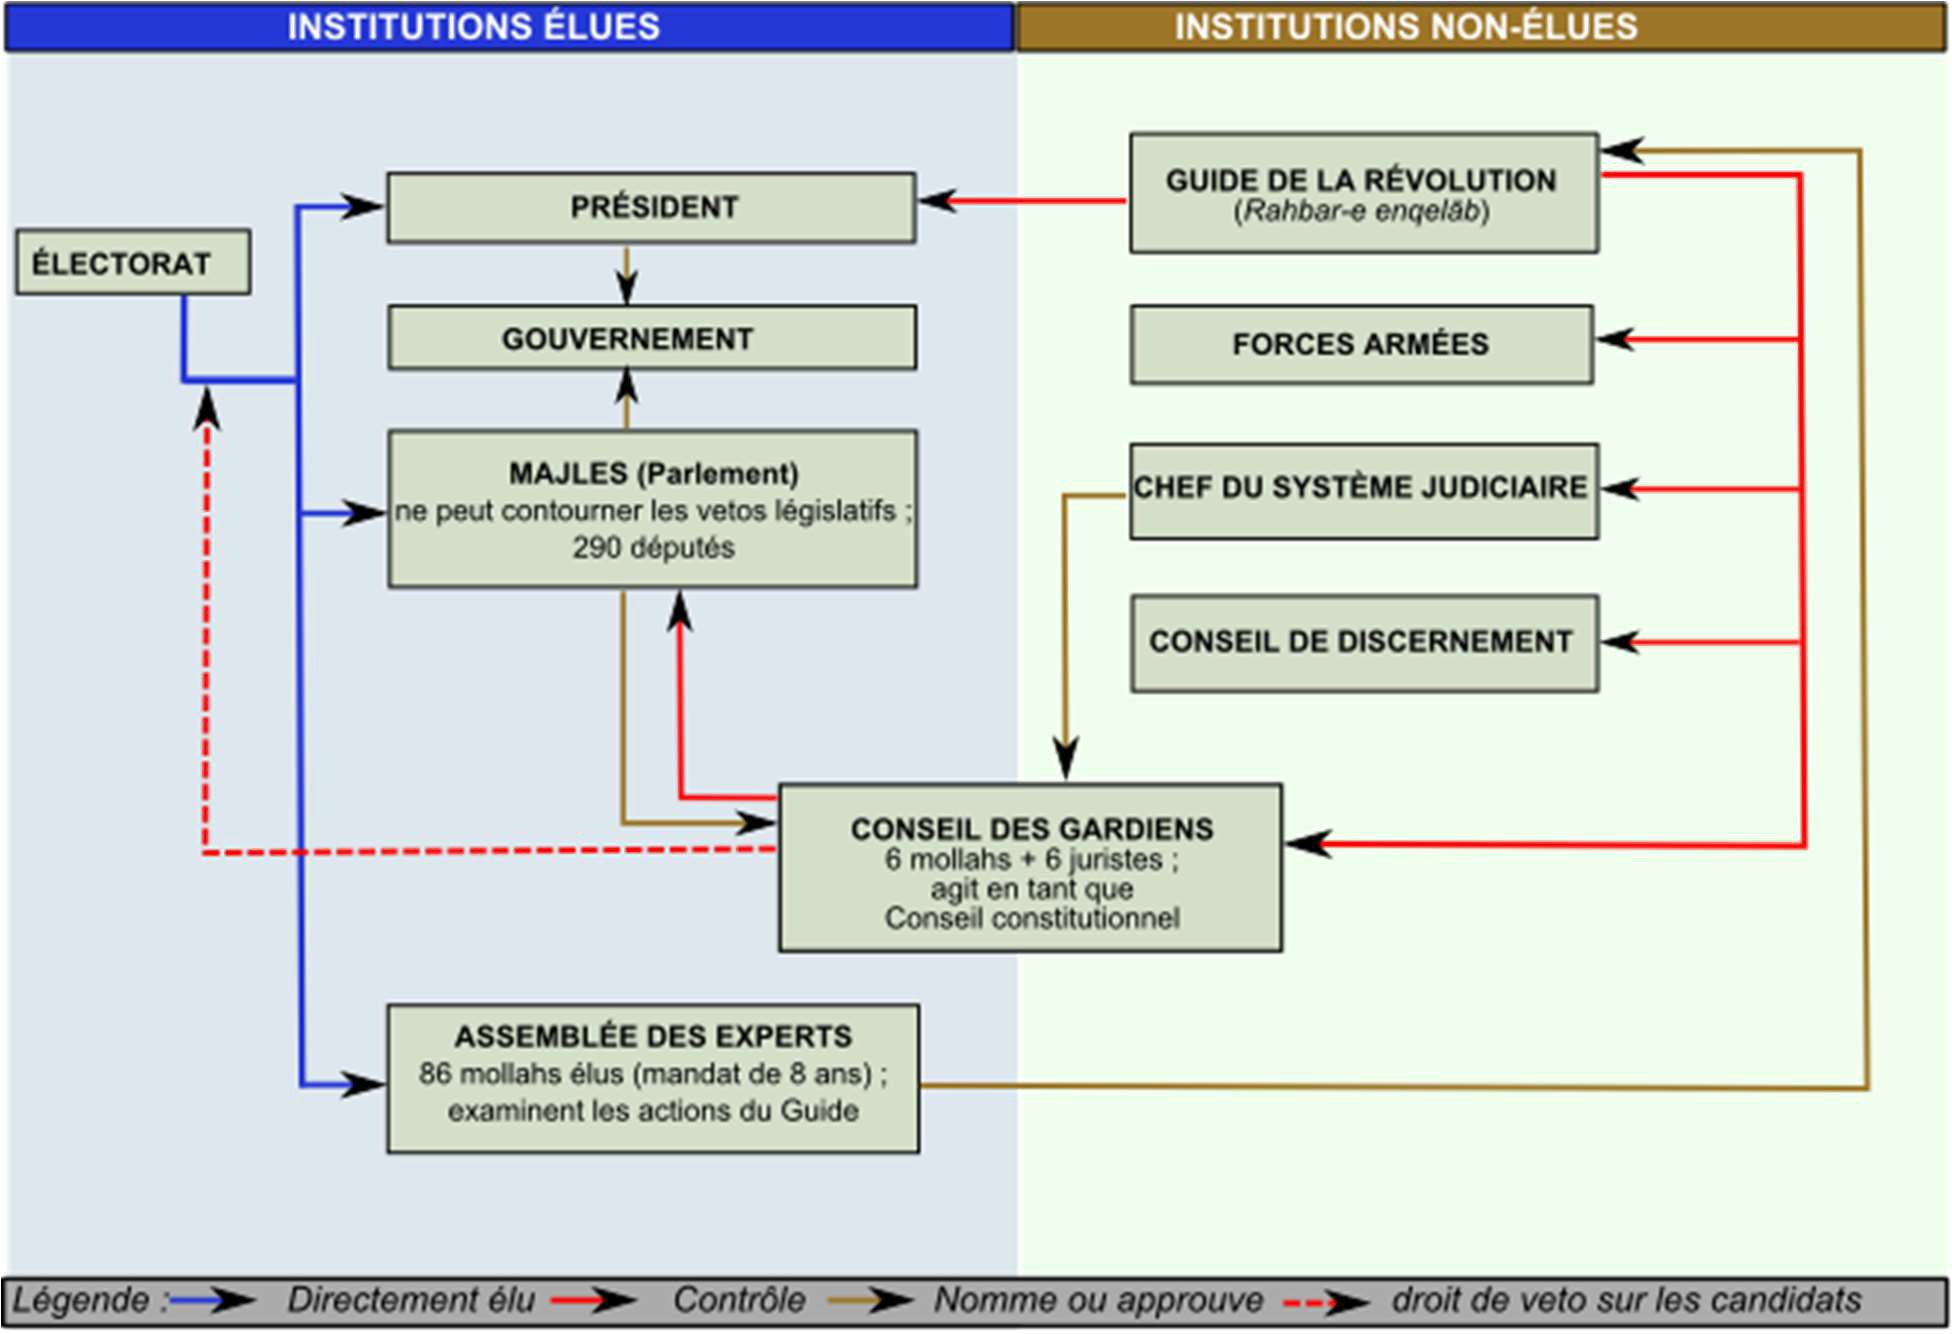
\includegraphics[width=\textwidth]{CourantsIslamContemporain/ImagesCourantsIslamContemporain/image3.jpeg}
  
    \label{fig:my_label}
\end{figure}
 

 





\hypertarget{glossaire-6}{%
\section{ {Glossaire}}\label{glossaire-6}}

 
\paragraph{Personnes}



Khameney Khatami

Khomeyni (Ruhollah) Mohammed Reza Shah Shariati (`Ali)

{Lieux} Jabal Amil Karbala Najaf

Neauphle-le-Château

\paragraph{Notions}

ayatollah : « \emph{signe de Dieu » (sur terre) ; grade supérieur dans
le clergé chiite}. marja'-ye taqlid : \emph{« source d'imitation » ;
plus haut grade dans le clergé chiite.} 



tawhid : \emph{unicité (divine).}

mujtahid : \emph{celui qui pratique l'ijtihad.}

musta`zafin : \emph{les opprimés.}





\chapter{La nouvelle pensée islamique}
\mn{\emph{(04/04/2022)}}


\section{Bibliographie}


\begin{itemize}
\item
  
  AL AJAMI, \emph{Que dit vraiment le Coran}, Erick Bonnier Editions,
  2020.
  
\item
  
  ABOU ZEID Nasr Hamid \emph{Critique du discours Religieux}, Sindbad,
  Acte Sud, Paris, 1999.
  
\item
  
  AL-BANNA, Gamal \emph{L'Islam, la Liberté, la Laïcité et le Crime de
  la tribu des « il nous a été rapporté »}, trad. D. Avon et A. Elias,
  L'Harmattan, Paris, 2013.
  
\item
  
  ARKOUN, Mohamed \emph{Lectures du Coran}, Maisonneuve \& Larose,
  Paris, 1982.
  
\item
  
  BAJRAFIL, Mohammed \emph{L'islam de France, l'an I. Il est temps
  d'entrer dans le XXIe siècle}, Ed. Plein Jour, 2015.
  
\item
  
  BENKIRANE Réda \emph{Islam, à la reconquête du sens}, éd. Le Pommier,
  2017.
  
\item
  
  CHARFI, Abdelmajid \emph{L'islam entre le message et l'histoire},
  Albin Michel, Paris, 2004.
  
\item


\emph{La pensée islamique, ruptures et fidélités}, Albin Michel, 2008.


 
\item
  
  CHEBEL, Malek \emph{Manifeste pour un islam des lumières}, Hachette,
  Paris, 2004.
  
\item
  
  ESACK Farid \emph{Coran, mode d'emploi}, Albin Michel, Paris, 2004.
  
\item
  
  LAMRABET Asma, \emph{Islam et femmes : les questions qui fâchent},
  Casablanca, En toutes lettres, 2017.
  
\item
  
  SANGARE, Youssouf \emph{Repenser le Coran et la tradition islamique --
  Introduction à la pensée de Fazlur Rahman}, Al Bouraq, 2017.
  
\item

  TALBI Mohamed \emph{Plaidoyer pour un Islam moderne}, Cérès/Tunis,
  DDB/Paris, 1998.
  

\item BENZINE, Rachid \emph{Les nouveaux penseurs de l'Islam}, Albin Michel,
Paris, 2004. FILALI-ANSARY, Abdou \emph{Réformer l'islam ? Une
introduction aux débats contemporains}, La
Découverte, Poche, Paris, 2005.

 \item HOFFNER, Anne-Bénédicte \emph{Les nouveaux acteurs de l'islam}, Paris,
Bayard, 2017.

\item RENAUD, Etienne "Mahmud Taha et la «seconde mission de l'Islam»",
\emph{Se Comprendre}, 85/07, 1985.

\item ROUSSILLON\textbf{,} Alain \emph{La pensée islamique contemporaine},
\emph{acteurs et enjeux}, Téraèdre, Paris, 2005.

\item SALEH Waël, \emph{A la recherche d'un aggiornamento de l'islam. Des
voies contemporaines}, Paris, L'Harmattan, 2018.

\end{itemize}



\section{Les nouveaux penseurs : essai
  de
  présentation}
  
  \subsection{Synthèse}
  
  \begin{Synthesis}
  Nous sommes dans un contexte Post moderne. A la différence moderne, universaliste et objectif, en post modernité, il n'y a qu'un accès relatif et subjectif à la vérité.
  Nous sommes tous des personnes raisonnables mais la façon d'accéder à la vérité, passe par le filtre de la subjectivité. 
  Le Coran passe par le filtre de la propre de subjectivité de Mohammed. Le texte est déjà une interprétation. Il y a une remise en cause du Coran \textit{Verbatim}.  
  \end{Synthesis}
  
Rachid Benzine \sn{voir p. \pageref{Theo:Benzine}}: 
\begin{quote}
    les modernistes, ou les nouveaux penseurs
\end{quote}  

Il s'est développé à partir des années 1980 en réaction à l'Islam politique et le wahhabisme, l'entrée de la violence en Islam, la cloture.

\paragraph{dans un cadre post moderne}
Ils vont chercher des nouvelles voies. La grande différence avec les modernistes, c'est qu'ils pensent la fin du XXeme. Ce n'est plus la positivité d'Auguste Comte, c'est le cadre de la post modernité. On reconnaît que la raison est construite historiquement, sociologiquement. L'accès à la vérité est donc partiel. Ce qui demeure et s'accentue, c'est la subjectivité.

\paragraph{L'herméneutique} ou Interprétation. L'accès à la vérité ne peut se faire que via l'herméneutique.

\begin{Def}[herméneutique]
Il n'y a que des interprétations à la vérité auxquelles on accède
\end{Def}

\paragraph{Conséquences} 
\begin{itemize}
    \item Il n'y a pas une essence de l'Islam. \textit{il n'y a que ce que les croyants musulmans en disent}.
    \item refus de chercher un islam pur à l'origine. Il n'y a que des islams contextualisés
    \item Importance plus faible du droit, de la norme. Ce qui compte, c'est l'éthique. L'Islam est moins pensé comme une religion normative mais un moyen pour l'individu d'entrer en relation avec le divin.
\end{itemize}

\paragraph{Rapport complexe à l'occident} Ils peuvent en particulier critiquer l'aspect absolu des droits de l'homme qu'il convient de contextualiser en Islam.

\paragraph{Un même type de formation} Plutôt formés en sciences humaines ou littératures, où ils ont découvert l'herméneutique : philosophie, histoire, ... acquis en occident. Ils prennent très au sérieux les études en sciences islamiques. 

\paragraph{En opposition avec les élites} religieuses (qu'ils critiquent) ou étatiques (face à leur souhait démocratique). Exil parfois nécessaire. En Tunisie et au Maroc, on pouvait avoir cette réflexion.

\paragraph{Du monde entier} 
\begin{itemize}
    \item Arabe
\begin{itemize} 
    \item Arkoun (Mohamed) (Algérie)
    \item Abu Zayd (Nasr Hamid) (Egypte)
    \item Khalafallah (Muhammad Ahmad) (Egypte)
\end{itemize}
\item Iran
\begin{itemize} 
    \item Sorush (Abdelkarim)
    \item Shabestari (Muhammad)
\end{itemize}
\item Pakistan
\begin{itemize} 
    \item Rahman (Fazlur)
    \item Engineer (Ali)
\end{itemize}
\item Afrique du Sud
\begin{itemize} 
    \item Esack (Farid) (théologie de la libération)
\end{itemize}
\end{itemize}
A classer : 
   Charfi
(Abdelmajid) 

 Hossein (Taha) Iqbal (Muhammad)

 

 
  
\section{Nouvelles approches critiques}

\subsection{L’approche littéraire}

Rappel du statut du Coran en Islam Classique : voix de Dieu et Mohammed n'est que l'enregistreur. Ce texte est vérité.

'Abduh va suggérer que le Coran ne doit pas être pris comme un document historique. Le but du Coran est d'exhorter les fidèles, sans avoir un soucis de précision historique.

\paragraph{Al-Khuli (Amin) 1895-1966} Enseigne à Al-Azhar. mais il a fait quelques années d'étude en Europe. Le Coran doit être compris et analysé comme un texte littéraire : 
\begin{itemize}
    \item Sémantique : les mots à l'origine. \sn{Ce n'est pas tout à fait nouveau. des les premiers siècles de l'islam, travaux sur la poésie pre-islamiques, la grammaire et dictionnaires}
    \item forme littéraire
    \item le contexte culturel et social. Cela est nouveau.
\end{itemize}

\paragraph{Khalafallah (Muhammad Ahmad) 1916-1998 } Disciple de Al-Khuli. Savant et étude de lettres à l'université du Caire (université moderne). Thèse en 1948 sur \textit{l'art du récit dans le Coran}. Il va aller jusqu'à dire que certains récits dans le Coran n'ont pas de valeur historique mais uniquement littéraire. 

\begin{Ex}
Par rapport aux récits des \href{https://fr.wikipedia.org/wiki/Sept_Dormants_d\%27\%C3\%89ph\%C3\%A8se#:~:text=Les\%20Sept\%20Dormants\%20d'\%C3\%89ph\%C3\%A8se,r\%C3\%A9cit\%20au\%20contexte\%20arabo\%2Dmusulman.}{sept dormants d'Ephèse}, va montrer que dans certains versets, il y en a 5 et dans d'autres 6. Cela montre que le but de Dieu n'est pas de faire un récit historique
\end{Ex}

Pour Khalafallah, il distingue dans le Coran différentes formes littéraires : 
\begin{itemize}
    \item Historique
    \item Parabolique : ce qui compte, c'est le message
    \item mythique (comme dans les sept dormants)
\end{itemize}

\subparagraph{une forte réaction à Khalafallah} car dès le Coran, on reprochait au Prophète de ne transmettre que des mythes. La réponse de Khalafallah a été de dire que le point du prophète était de défendre que ces textes étaient révélés. Thèse refusée et \textit{fatwa} interdisant à Al-Khuli et Khalafallah d'enseigner les sciences coraniques. Thèse néanmoins publiée.


\subsection{Critique historique}

\paragraph{Mohammed Arkoun 1928 - 2010} \label{theol:Arkoun5} En France en 1954, agrégé d'arabe\sn{cf p. \pageref{theol:Arkoun1}}. Il est marqué par la pensée des IX-X siècle. Sa compréhension de l'Islam (comme dans toute religion) : 
\begin{itemize}
    \item \textbf{la religion forte} réponse théologique crédible aux grandes questions de l'homme : le bien, le mal, ce qui se passe après la mort,... C'est ce qui compte pour toute grande religion
    \item \textbf{religion individuelle} la façon dont une religion se déploie à l'intérieur de chaque individu dans sa vie intérieure et sa relation à Dieu
    \item \textbf{la religion forme} les formes prises par la Religion dans une situation sociologiques et historiques données. Pour lui secondaire. 
\end{itemize}

\subparagraph{Une sacralisation de la religion forme} en Islam :
\begin{itemize}
    \item sur le plan politique, le \textit{califat}
    \item sur le plan politique, la \textit{shari'a}, loi religieuse
    \item et \textit{l'umma} éventuellement pouvant être pensé comme un seul état.
\end{itemize}
Si on touche à l'un de ces trois points, on touche à ce qui est considéré comme coeur à l'islam

\subparagraph{il faut une archéologie pour déconstruire ces formes}  L'Islam aurait pu être autre que ce qu'il est aujourd'hui. Ce sont des rapports de force qui ont imposé le califat, la shari'a et l'umma. 
\subparagraph{Une cloture dogmatique} au X-XI eme siècle. Ce qui est pensable et ce qui est impensable (tabou). Par exemple :
\begin{itemize}
    \item on oublie la genèse du texte du Coran. Simplification alors qu'on sait
    \item Coran incréé.
\end{itemize}
Il y a en parallèle un imaginaire, celui de l'âge d'or des 4 premiers califes, qui permet de justifier cette fermeture.

Arkoun va même jusqu'à distinguer le fait coranique de la révélation et le document historique et littéraire, le \textit{corpus officiel clos} qui est lui le résultat d'un rapport de force. 
\begin{Ex}
Osman a fait brûler des corpus hétérodoxes.
\end{Ex}


\paragraph{Différence entre les modernistes et les réformismes} Les modernistes critiquent la trahison des premières générations, à l'opposé de ce qui est reçu par la tradition musulmane d'un âge d'or.



\section{le statut de la Parole de Dieu : un Coran créé ?}



\subparagraph{Le statut du Prophète }

\paragraph{F. Rahman 1919-1988} Indo Pakistanais. Formation moderne. Inde puis Oxford (th. Philosophie). Enseigne au Canada. Rentre au Pakistan en 1961 mais il va rencontrer une très forte contestation des savants pakistanais. Ils vont l'accuser d'apostasie. Exil aux US en 1968 où il connaît une célébrité.

\paragraph{Une vision du Coran où le Coran passe par la langue et l'imaginaire du Prophète}. Voir texte. Un Coran purement extérieur du fait des controverses chrétiennes (lo-
gos,...) La parole de Dieu mais elle est aussi parole du prophète (dans
son coeur) et pas seulement enregistreur. Il reconnaît une subjectivité du
Prophète. Elle s’incarne dans son imagination, sa langue,...


\paragraph{Coran Parole de Dieu}\sn{Fazlur Rahman
(1919-1988) \emph{Extrait de son livre \textbf{Islam} (Doubleday Anchor Book, New
York, 1968, 331 pp.), p. 25-28.}}

 \begin{quote}
     

Pour le Coran lui-même, et par conséquent pour les Musulmans, le Coran
est la Parole de Dieu (kalâm Allâh). Mohammed, lui aussi, était
absolument convaincu de recevoir le Message de Dieu, le Tout-Autre (nous
essaierons plus loin de comprendre plus précisément le sens de cette
Altérité absolue), à tel point qu'il s'est basé sur la force de cette
conviction pour rejeter quelques-unes des assertions historiques les
plus fondamentales de la tradition Judéo-Chrétienne concernant Abraham
et les autres Prophètes. Cet "Autre", par un certain canal, a "dicté" le
Coran avec une autorité absolue. La voix surgissant des profondeurs de
la vie parlait distinctement, impérieusement, sans méprise possible. Non
seulement le mot \textbf{"}\emph{qur'ân}", signifiant "récitation",
l'indique clairement, mais le texte du Coran lui-même déclare en
plusieurs endroits que le Coran est révélé verbalement et non pas
seulement son "sens" et ses idées. Le terme coranique pour "Révélation"
est \emph{wahy} dont le sens est assez proche d' "inspiration", à
condition que ce mot ne soit pas censé exclure nécessairement le mode
verbal (par "Parole", bien entendu, nous ne voulons pas dire le Son). Le
Coran dit: "Dieu ne parle à aucun humain (c'est-à-dire en paroles
audibles) excepté par \emph{wahy} (c'est-à-dire par idée-parole,
inspiration) ou derrière un voile, ou bien Il envoie un Messager (un
ange) qui parle par \emph{wahy}...Nous t'avons ainsi révélé un Esprit
qui est à nos ordres". (Q. 42,51-52)


Pendant le 2° et le 3° siècles de l'ère islamique, cependant, de
violentes différences d'opinion, des controverses, en partie causées par
l'influence des doctrines chrétiennes, s'élevèrent parmi les Musulmans
au sujet de la nature de la Révélation. L'"orthodoxie" islamique
émergente qui en était au point crucial de formuler son contenu précis,
mit alors l'accent sur l'origine externe de la Révélation Prophétique
afin d'en sauvegarder son "Altérité", son "Objectivité" et son caractère
verbal. Le Coran lui-même maintenait certainement son altérité vis-à-vis
du Prophète. Il déclare en effet: "\emph{L'Esprit fidèle l'a fait
descendre sur ton coeur pour que tu sois au nombre des avertisseurs}"
(Q. 26,194), et encore: "\emph{Dis: Qui est l'ennemi de Gabriel (qu'il
le soit), car c'est lui qui a fait descendre sur ton coeur... le Livre}"
(Q. 2,97). Mais il manquait à l'orthodoxie (en fait, à toute la pensée
médiévale) d'avoir les instruments intellectuels nécessaires pour
allier, dans sa formulation du dogme, l'Altérité et le caractère verbal
de la Révélation d'une part, et, d'autre part, son lien intime avec
l'oeuvre et la personnalité religieuse du Prophète, c'est-à-dire qu'il
lui manquait la capacité intellectuelle de dire, à la fois, que le Coran
est entièrement la Parole de Dieu et aussi, dans un sens ordinaire, la
parole de Mohammed. Le Coran affirme clairement les deux idées, car s'il
insiste sur le fait qu'il est descendu sur le "coeur" du Prophète,
comment peut-il lui être extérieur ? Ceci, bien sûr, n'implique pas
nécessairement que le Prophète ne percevait pas un personnage extérieur,
comme la tradition le dit, mais il est remarquable que le Coran lui-même
ne fait aucune mention d'un personnage dans ce contexte: ce n'est qu'en
lien avec certaines expériences (habituellement liées à l'Ascension du
Prophète), que le Coran parle du prophète comme de quelqu'un ayant vu un
personnage ou un esprit ou quelque autre objet "à la lointaine limite"
ou "à l'horizon" bien qu'ici encore, comme nous l'avons dit,
l'expérience soit décrite comme étant d'ordre spirituel. Mais
l'orthodoxie, par les \emph{hadith} ou les "traditions" transmises du
Prophète, en partie interprétées correctement, et en partie inventées,
ainsi que par une discipline théologique largement basée sur le
\emph{hadith}, fit de la Révélation prophétique un phénomène ne frappant
que son oreille, uniquement extérieur à lui, considérant l'ange ou
"l'esprit qui vient sur le cœur" comme un agent totalement externe.
L'image que l'Occident moderne garde de la Révélation prophétique se
base largement sur cette formulation orthodoxe plutôt que sur le Coran,
d'ailleurs la foi du Musulman ordinaire fait de même.

... Lorsque la perception intuitive de la morale chez Mohammed atteint
son plus haut point et s'identifie avec la morale elle-même, la Parole
est donnée avec l'inspiration elle-même. Le Coran est donc la pure
Parole divine, mais évidemment, il est également relié intimement à la
personnalité interne du Prophète Mohammed, dont la relation au Coran ne
peut être conçue mécaniquement comme un disque enregistré. La Parole
divine passe par le cœur du Prophète.
 \end{quote}


\begin{Synthesis}
Un Coran purement extérieur du fait des controverses chrétiennes (logos,...)
La parole de Dieu mais elle est aussi parole du prophète (dans son coeur) et pas seulement enregistreur. Il reconnaît une subjectivité du Prophète. Elle s'incarne dans son imagination, sa langue,...
\end{Synthesis}

\subsection{L’ « abaissement » de la Parole }
\paragraph{Abu Zayd (mort en 2010)} Littérature arabe en Egypte et étude aux USA. Approche littéraire. Une langue est forcément porteuse d'une culture donnée, une langue particulière. Il va jusqu'à parler d'une \textit{incarnation de la Parole}, une langue humaine. Si Dieu a choisi l'arabe, il faut étudier ce texte en Arabe comme n'importe quel texte littéraire. 

\subparagraph{Contextualisation culturelle}

\section{la question de l'interprétation}

\subsection{Approche littéraire} 
Avec Abu Zayd.
Tout texte demande à être reçu et interprété, il ne vit pas en soi. C'est le passage, la transformation par la subjectivité de l'auditeur. Et ce texte coranique est \textit{marqué par l'interprétation du Prophète}. Il va comparer le Coran à un organisme vivant qui est riche d'une infinité de sens et qui va se donner selon la compréhension de l'auditeur.

\paragraph{des critères pour interpréter}


\begin{itemize}
    \item Sens : sens qu'avait le texte pour le prophète et ses compagnons
    \item signification : sens pour aujourd'hui
\end{itemize}
Le critère est de s'assurer de la \textit{cohérence entre sens et signification}. 


\subsection{Approche scientifique }

\paragraph{A. Sirush 1945-} Approche par la philosophie des sciences. Il a découvert la philosophie des sciences; Thèse en Angleterre. Très enthousiaste au début de la révolution en Iran. Il s'est exilé aux US (Harvard).

\paragraph{Un parallèle entre nature/science et religion} A. Sirush fait un parallèle entre nature et science d'une part et Religion et ce qu'il nomme religiosité d'autre part:
 
\begin{tabular}{p{5cm}p{1cm}p{5cm}}
Nature &  & Religion   \\
\textit{{objectif, absolu} }      \\                        
          $ \downarrow $  &  &         $ \downarrow $  \\
Science &  & Religiosité\\
\textit{{partielle, mouvante}}  & & \textit{ce que nous comprenons de la religion} \\
\end{tabular}
 


\paragraph{théorie de l'extension et de la contraction de la connaissance religieuse}, la religiosité. Tout est lié, toute découverte sur les sciences a un impact sur notre philosophie et l'anthropologie, et donc ensuite sur notre compréhension.


\begin{Ex}
L'Eglise s'est opposée à l'idée que la terre tournait autour du soleil. Car cela changeait notre regard de la place de l'homme et de la création, au centre et au sommet de la Création.
\end{Ex}

\paragraph{un processus continu} de connaissance religieuse. Notre compréhension de la religion évolue. Il faut être dans une attitude de questionnement pour que le Coran parle. 
\begin{quote}
    Si l'homme n'a aucune question à poser au religieux, il ne vient apprendre de ce religieux. \ldots Même chose pour le Coran.
\end{quote}

\paragraph{Pluralisme de pensée}
Cela a des implications politiques et démocratiques. Dialogue.

\subsection{Glossaire}

 
{Personnes}



{Notions}
\begin{Def}[tafsir]
\emph{commentaire (exotérique) du Coran}
\end{Def}


\begin{Def}[ta'wil]
\emph{herméneutique ésotérique du Coran}
\end{Def}
 


\chapter{Evolution de l'interdiction du \riba et Gharar}


a. Un dossier sur un thème lié au cours A partir de trois articles universitaires minimum. -  Introduction : intérêt du thème au regard de l’actualité et/ou de vos propres orientations personnelles ; présentation des articles et de leurs auteurs. Présentation du plan de votre travail. - Synthèse (ne pas présenter les articles séparément mais faire une synthèse à partir des différentes thématiques rencontrées) - Contextualisation de ce thème dans l’islam contemporain, éclairage par le contenu du cours (enjeux, dynamiques, etc). 

\section{Introduction}

En tant que membre du jury de l'Institut des Actuaires, j'ai eu à me prononcer sur certains mémoires présentés par des étudiants sur la \textit{finance Islamique} et \textit{l'assurance Takaful}. Ces mémoires ne couvrent pas les présupposés théologiques et commencent généralement par une présentation des interdits de la loi musulmane, comme par exemple ce \href{http://www.ressources-actuarielles.net/EXT/ISFA/1226-02.nsf/0/8c814ff5f2bae57ec1257e1a004407b6/\%24FILE/Memoire_ISFA_Tontines_et_Takaful_Bendimerad_Version_avec_Couverture.pdf}{mémoire d'actuariat} : 
\begin{quote}
     [pour faire face à ses  engagements, l'assureur],peut, par exemple, inclure des actifs obligataires dont les taux de rendement font apparaître des taux d'intérêt. [...] l'interdiction de l'usage du taux d'intérêt, appelé \textit{\riba} en arabe, est l'un des fondements du droit des affaires musulman.
\end{quote}
Dans la même veine, sont généralement définis les autres interdits, comme le \emph{Gharar}, défini dans le même mémoire comme : 
\begin{quote}
    Le contrat d'assurance peut constituer une perte disproportionnée en faveur de l'un des participants aux dépens de l'autre. Ce caractère d'incertitude, appelé \textit{Gharar} en arabe, est un caractère prohibé par l'Islam surtout lorsque le transfert du risque vers un tiers est total, ce qui est notamment le cas pour l'assureur qui porte entièrement la charge du risque cédé par l'assuré.
\end{quote}
Les mémoires d'actuariat consultés essayent de dépasser ces interdictions, qui soulignent une tension avec les \textit{Hadiths} : 

\begin{quote}
     
A l'issue de l'analyse précédente, l'idée même d'une assurance islamique semble être un contresens. Pourtant, la religion musulmane encourage l'individu à prendre des mesures pour réduire l'ampleur des désastres qui pourraient l'affecter. D'après un Hadith authentifié, le prophète conseille à un croyant de placer sa confiance en Dieu et d'attacher son chameau plutôt que de se limiter uniquement à placer sa confiance en Dieu en offrant la possibilité au chameau libre de s'échapper. L'Islam ne s'oppose donc pas à l'idée de vouloir minimiser les risques et par conséquent elle ne s'oppose pas à faire usage de la loi des grands nombres. Elle exclut certes la spéculation et l'incertitude ainsi que le taux d'intérêt. En revanche, elle compte parmi ses principes la coopération et l'entre-aide mutuelle ainsi que le partage équitable des risques et des bénéfices. Toutes ces bases ont permis de concevoir un modèle alternatif à celui de l'assurance conventionnelle.
\end{quote}
De cette tension naît des solutions techniquement assez complexes.


Intrigué par cette apparente clarté vis à vis de l'interdiction de l'\textit{intérêt} et de l'\textit{l'incertitude} à la base de l'économie moderne, je me propose d'étudier l'évolution de l'opposition de la \emph{\riba} et \emph{gharar} dans les différents courants de l'Islam contemporain, depuis la pensée d'Abduh jusqu'aux frères musulmans et le salafisme. 
L'interdiction des deux notions n'a pas la même importance économique et la \textit{\riba} a donné lieu à plus de développement. En partant de ces études, j'essayerais néanmoins de transposer ces travaux à l'assurance.
Après avoir regardé  à travers l'étude de ces deux notions comment l'économie moderne, pensée au XVIIIè et XIXè siècle questionne l'Islam, je poserai quelques pistes sur le propre questionnement du Christianisme. Après tout, le prêt à intérêt était aussi interdit au Moyen-äge en Europe (Concile de TOurs de 1163). Ces pistes seront en particulier nourries par l'étude de la pensée de Saint Thomas d'Aquin sur les taux d'intérêt et comment ces pistes peuvent nourrir la réflexion de la théologie musulmane (et chrétienne) contemporaine. 
 

%---------------------------------------------------------------------------------------------------------------
\section{Vision dans l'Islam Classique de l'interdiction de \riba}

\subsection{une interdiction de la \riba et Gharar}

Pour commencer, il est utile de se référer aux textes à l'origine de ces interdits.
\paragraph{Versets du Coran et Hadiths interdisant la \riba}
Le verset 130 de la Sourate 3, Al-Imran mentionne : 
\vocalize % switch diacritics for short vowels on
\transtrue % display the transliteration
\arabtrue % print arabic text (on by default)
\begin{quote}
 
\TArabe{
 يَا أَيُّهَا الَّذِينَ آمَنُوا لَا تَأْكُلُوا الرِّبَا أَضْعَافًا مُّضَاعَفَةً وَاتَّقُوا اللَّهَ لَعَلَّكُمْ تُفْلِحُونَ
  } 
   [3,125] O vous qui croyez !, ne vivez pas de la \textit{\riba} [produisant le] double deux fois ! Soyez pieux envers Allah ! Peut-être serez-vous bienheureux. 

\end{quote}
\begin{quote}
\TArabe{278
 يَا أَيُّهَا الَّذِينَ آمَنُوا اتَّقُوا اللَّهَ وَذَرُوا مَا بَقِيَ مِنَ الرِّبَا إِن كُنتُم مُّؤْمِنِينَ
279 فَإِن لَّمْ تَفْعَلُوا فَأْذَنُوا بِحَرْبٍ مِّنَ اللَّهِ وَرَسُولِهِ وَإِن تُبْتُمْ فَلَكُمْ رُءُوسُ أَمْوَالِكُمْ لَا تَظْلِمُونَ وَلَا تُظْلَمُونَ
} 
 [2, 278] O vous qui croyez !, soyez pieux envers Allah ! Faites abandon de ce qui [vous] reste [à toucher provenant] de la \textit{\riba}, si vous êtes croyants !
[2, 279] Si vous ne le faites point, attendez-vous à une guerre de la part d’Allah et de Son Apôtre ! si vous vous repentez, alors vous récolterez votre capital sans infliger ou être victime d’une injustice. \sn{Traduction de Blachière, sauf la dernière phrase \cite{ElGamal:BanqueFinanceIslamique}}

\end{quote}

De même, un hadith de Abu Hurayra met au même niveau la \textit{\riba} et le meurtre : 
\begin{quote}
    "Evitez les sept turpitudes !"

- "Quelles sont-elles, ô Envoyé d'Allah?", demandèrent les fidèles.


- "Ce sont, répondit-il :

 

-le polythéisme,

-la magie,

-le meurtre qu'Allah a interdit sauf à bon droit

-l'usurpation des biens de l'orphelin,

-la \textit{\riba},

-la fuite du front au jour du djihad et

-la fausse accusation (de fornication) des femmes vertueuses, chastes et croyantes".
\end{quote}
 
  Nous avons évité à ce stade de traduire le terme de \textit{\riba}, par \textit{usure} ou \textit{intérêt}. Le Hadith rapport par at-Tirmidhî a été utilisé pour appliquer le sens d'intérêt à la \textit{\riba}  : 
 \begin{quote}
     Vendez de l'or contre de l'argent (les quantités échangées étant) comme vous voulez, à condition que ce soit main à main. Vendez du blé contre des dattes sèches (les quantités échangées étant) comme vous voulez, à condition que ce soit main à main. Vendez de l'orge contre des dattes sèches (les quantités échangées étant) comme vous voulez, à condition que ce soit main à main (n° 1240)
 \end{quote}  
 On peut effectivement y lire le refus de l'intérêt mais d'autres lectures sont possibles, en particulier en relevant l'insistance du hadith à une transaction \textit{main à main}, qui permet une transaction claire. Par ailleurs, la valeur du temps n'est pas explicitement mentionnée.
 

 
\subsection{un nouveau contexte avec la naissance du Capitalisme}
Du point de vue du prêteur, le prêt à un prix du fait du risque  que l'emprunteur repaye le prêt, la valeur temps (qui correspond à l'inflation et à la perte d'opportunité d'un investissement aujourd'hui qui rapporte plus plus tard). La pertinence économique de l'intérêt et de la prise de risque est donc justifiée même si cela ne veut pas dire qu'elle l'est d'un point de vue religieux.
Avec l'accumulation des richesses dans les villes italiennes au moyen-âge naît le capitalisme et la finance : comment financer et assurer les bateaux partant de Gênes et remplis de richesse ? Cette irruption de la finance pose de nouvelles questions.  Face à cette accumulation, une réponse théologique chrétienne sera la création de l'ordre mineur par Saint François d'Assise. Et, nous reviendrons sur ses développements, la réflexion de l'université de Paris et de Saint Thomas d'Aquin sur la notion d'usure et de juste prix.  
Ces innovations touchèrent tardivement le monde musulman, au XIXème, avec l'arrivée simultanée de l'industrialisation, qui nécessite des capitaux importants et les débuts de la colonisation. Par l'industrialisation, la capacité productive est fortement augmentée par l'investissement, mais aussi la concentration des risques qui ne peuvent être portée par la solidarité traditionnelle.
Face à cette nouvelle question, quelles sont les réponses proposées par les théologiens musulmans depuis l'arrivée de cette question ?


%---------------------------------------------------------------------------------------------------------------
\section{Elements théologiques apportés}

\subsection{Premières réponses face à la nécessité du prêt}
\paragraph{Le développement du \riba et de l'assurance par les Occidentaux} Les prêts à intérêt ont toujours existé au sein de l'Empire Ottoman\cite{Gilbar:Qadi}, et proposés par des familles grecques, arméniennes ou Juives (et en Iran par les arméniens et zoroastriens). A ce premier Groupe, s'ajouta les banques commerciales européennes ou les banques "étrangères-locales" comme la banque impériale ottomane au XIX.
De la même façon pour les assurances, Ibn Abidin, représentant de l'école officielle de droit Hanadi dans l'empire ottoman, suggère le compromis suivant : il est licite d'établir ds contrats d'assurance portant sur les risques encourus à l'intérieur du royaume islamique - le Dar al Islam -à condition que ces contrats soient conclus avec une compagnie d'assurance ayant son siège hors de pays de l'Islam. 

\paragraph{Utilisation de prêt à intérêt par les musulmans malgré l'interdiction du \textit{\riba}.} La \textit{\riba} a pu poser des problèmes dans son implémentation, en particulier pour les grands marchands (tujjār).  
Pour l'école Hanafite, le terme de \riba peut être traduit par usure, dans le sens d'un taux d'intérêt exhorbitant, à l'opposé de l'intérêt raisonnable, le \emph{ribh}. L'autre interprétation dominante, attribuée à 'Abdahallah Ibn 'Abbas, permet d'expliquer la notion du Coran de double capital par la pratique du \textit{\riba al jâhiliyya} (préislamique), avec des taux d'intérêt très élevés avec des intérêts pouvant dépasser le capital en cas de non-paiement. A l'opposé de ces analyses plus ouvertes, la position de l'école Hanbalite fut l'interdiction pure de l'intérêt. Pour contourner l'interdit du \riba face à la nécessité, les marchands musulmans mirent en place des montages complexes où l'intérêt était déguisé en une \textit{double vente} (\emph{mukhâtra}) avec deux ventes fictives successives permises par la \textit{sha'ia}: 
\begin{itemize}
    \item la première, le préteur vent un objet à l'emprunteur pour une somme équivalente au capital et à l'intérêt. l'emprunteur s'engage à payer la valeur de l'objet à la fin de la période (techniquement, une vente avec paiement différé). 
    \item A la fin de cette première transaction, l'emprunteur revend le même objet pour la valeur du principal (techniquement, une vente à terme).
\end{itemize}
 Cependant, l'étude des jugements des cours religieuses au moyen-orient entre le XVI et le XVIII montre que malgré ces montages, des exemptions partielles ou totales de paiement de l'intérêt du fait de son incompatibilité avec l'Islam \sn{GILBAR, GAD G. “The Qadi, the Big Merchant and Forbidden Interst (Ribā).” British Journal of Middle Eastern Studies, vol. 39, no. 1, 2012, pp. 115–36, http://www.jstor.org/stable/23264404. Accessed 3 May 2022.}
 

\section{la pensée d'Abduh et Rida}
\subsection{position d'Abduh} Le Cheikh {Muhammad Abduh} (1849 - 1905) Egyptien, successeur d'Al Afghani, est la figure marquante du réformisme islamique. Il s'oppose au colonialisme atteignant alors l'Egypte. Son séjour  parisien le convainc de la nécessité de réforme de l'Islam et l'initie aux réflexions intellectuelles occidentales et en particulier François Guizot. A sa suite, il il pense l'Islam comme civilisation et pas uniquement comme Religion, avec la notion de progrès lié à la civilisation. Il n'y a pas d'opposition pour lui entre Foi et Raison, la religion musulmane étant \textit{raisonnable}.    Dans son livre \citet{Abdou:Rissalat}, il part de la Raison pour montrer le besoin que l'homme ne se fixe pas sa propre loi.

Il montre tout d'abord la naissance des besoins et des liens entre les hommes. Idéalement ces liens seraient ceux de l'amour : 
\begin{quote}
    Nul ne met en doute que chaque membre d'une société a besoin
des autres membres; et chaque fois que l'individu accroître ses exigences
dans la vie il ressent plus fortement le besoin de recourir au concours
de ses semblables. Ainsi se développent les besoins et à leur suite s'étendent
les relations de la famille à la tribu, de celle-ci à la nation, et finalement
au genre humain tout entier, comme le montre notre époque . Ces
besoins qui créent dans le sein de chaque nation (surtout dans le sein de
celles qui méritent vraiment ce nom) des relations et des rapports
spéciaux la distinguant des autres nations, sont le besoin de se procurer
sa subsistance, celui de profiter des biens de la vie, celui d' acquérir
les choses désirables et d'éloigner de soi celles qui déplaisent. 
Si la vie de l'homme se déroulait selon les lois de la nature, telles
que nous les voyons appliquées aux autres êtres vivants, les besoins
que nous venons de citer auraient été parmi les facteurs les plus puissants
de l'amour entre les individus[...].  

[\ldots]
Si par contre, l'intérêt se mêle aux relations amicales, et si chacun des amis exige un prix pour son amour, celui-ce se change en esprit d'exploitation, il se reporte sur l'effet utilitaire et se transforme chez l'un des amis en un abus de la force, et chez l'autre, en peur avilissante, en dissimulation et en hypocrisie.
\cite[p.66]{Abdou:Rissalat}
\end{quote}
Mais l'homme ne vient pas selon les lois de la nature car il est inconstant : 
\begin{quote}
 l 'homme
a été créé avec un caractère inconstant; quand le malheur l'atteint
il est abattu, et quand il acquiert quelque bien il devient insolent.
(C. ch. 70, v. 19 à 21). [...]
Chaque fois que la mémoire et l'imagination les poussent à
éviter quelque chose qui leur inspire de la crainte ou à atteindre un
objet qui leur fait envie, leur intelligence leur ouvre une porte de la
ruse ou leur découvre une voie de la violence ; alors le rapt remplace
l'échange pacifique, la dispute prend la place de l'union et la conduite
de l'homme riche s 'appuie plus que sur l'astuce et la violence.
\cite[p 68]{Abdou:Rissalat}
\end{quote}
il montre qu'on peut accéder à l'équité par des voies naturelles mais qu'à la foi pour les masses et pour éviter la corruption des élites, il est nécessaire de s'appuyer sur loi externe.
\begin{quote}
[...] ] le genre humain
a surtout besoin, pour conserver son existence, de l'amour ou d'un
sentiment qui le remplace.
A différentes époques il y a eu des penseurs qui ont fait appel à
l'équité ; ils ont pensé, et même quelques mystiques ont exprimé cette
pensée par de nobles paroles, que l'équité remplace l'amour. Cette
assertion ne manque pas de sagesse, mais qui est-ce qui peut établir les
règles de l'équité et amener la totalité des hommes à se soumettre ?
\cite[p 69]{Abdou:Rissalat}
\end{quote}

Suivre la Loi de Dieu, ordonner le bien est alors supérieur à la foi : 

\begin{quote}
  le Coran indique
qu'il n'y a pas de condition meilleure que celle des hommes qui ordonnent
le bien et défendent le mal: \begin{quote}
    Vous êtes les meilleurs parmi les hommes,
vous ordonnez le bien, vous défendez le mal et vous croyez en Dieu. (Cor. ch. 3, v. 106.) 
\end{quote} 
 
Dans ce verset le fait d'ordonner le bien et de
défendre le mal est mentionné avant la foi en Dieu, bien que la foi soit la base même sur laquelle s'appuient les bonnes oeuvres. 
\cite[p 121]{Abdou:Rissalat}
\end{quote}

\paragraph{Conséquence pratique pour la \riba}
'Abduh liste alors une liste de maux que l'Islam permet d'éviter : 
\begin{quote}

[l'Islam] nous invite par dessus tout à dépenser notre bien pour les oeuvres
charitables et souvent il en fait l'expression de la foi et la manifestation
d'une bonne conduite; il déracina par là, du coeur des pauvres, la rancune
et la haine contre ceux que Dieu a favorisé des biens terrestres ; il leur
inspira l'amour pour les riches, tout comme il fît naître dans le coeur de
ceux-ci la pitié pour les malheureux ; ainsi il développa la confiance dans
le coeur de tous les hommes. Quel remède plus efficace contre les maux
dont souffre la société: « C'est une faveur que Dieu accorde à qui il veut,
car Dieu est d'une bienfaisance sans bornes. » (Cor. ch. 57, v. 21.)
\textbf{L' Islam a fermé les deux portes du mal, il a bouché les deux sources
qui minent l'intelligence et détruisent la richesse, en frappant les boissons
enivrantes, les Jeux de hasard et l'usure, d'une interdiction absolue qui
n'admet pas d'infraction.}
\cite[p 122]{Abdou:Rissalat}
\end{quote}
Ainsi, parmi ces maux figure la \riba traduit ici par \textit{usure}.

\paragraph{Pratiquement : l'avis d'Abduh sur l'ouverture de la Caisse d'Epargne en Egypte}
L'ouverture de la Caisse d'Epargne et la répugnance d'un certain nombre de musulmans à toucher les intérêts poussèrent la caisse d'épargne à demander à 1903 une Fatwa à Abduh \cite{Jomier:AdbouCaisseEpargne}. Cette fatwa semble n'avoir jamais existé. En revanche, Ce fut à la requête d'un particulier mais en fait pour la
Compagnie d'Assurances sur la vie Gresham. La Compagnie d'Assurances al-Chark,
au Caire,  conservait une copie d'une fatwa d'Abduh \textit{écrite initialement pour un particulier} afin de la montrer à ses clients, le cas échéant. Le
client effectue des versements réguliers et périodiques par tranches successives
prévues d'avance ; la compagnie les encaisse et se charge de faire fructifier cet
argent. Finalement, à l'échéance, la société remboursera le total des versements
effectués augmenté des bénéfices résultant de la fructification. La fatwa admet
la licéité d'une telle opération en des termes qui, au fond, s'appliqueraient à toute
société en commandite. Il faut noter que la revue Al-Manâr de \textit{Rashid Rida} ne nia pas l'authenticité de cette fatwa après la mort d'Abduh mais protesta contre l'extension faite à toute assurance vie.

\paragraph{la note de la revue Al-Manâr de 1903}


Face aux scrupules de 3000 musulmans à toucher les intérêts (fa'ida), un échange eu lieu entre le directeur de la Caise d'Epargne et Abduh, échange repris par la revue \textit{Al-Manâr}. Abduh y maintenait fermement le principe de
l'interdiction absolue de l'usure (al-ribâ) ; mais il ne classait pas le cas de la Caisse
d'Epargne avec ceux de l'usure. Il l'assimilait à celui d'une société en commandite
(chirkat al-mod'âraba). A la suite de cette discussion, la loi fut modifiée en 1904 : 
 

\begin{quote}
 Il est prévu dans l'article premier que le client devra signer un
formulaire imprimé dans lequel il déclarera donner au Directeur Général de la
Poste tout pouvoir pour faire fructifier les sommes déposées, d'une façon licite et
en excluant toute opération usuraire. Il déclare permettre au Directeur de la Poste
de joindre ses dépôts à ceux des autres clients pour les faire fructifier en commun
à condition de recevoir une part de bénéfices (al-ribh') proportionnelle à ses
versements. On notera que dans cet article comme dans tout le reste de la loi le
mot de \textit{fâ'ida}, intérêt, est totalement absent. \cite{Jomier:AdbouCaisseEpargne}
\end{quote}

\begin{quote}
    L'article deux stipule entre autres ce qui suit. Il évite de parler de tant pour
cent, formule qui rappelle trop les intérêts. Il note que la part des bénéfices ne
dépassera pas un pour quarante du capital et le surplus, s'il y en a, reviendra à
l'administration postale à titre de compensation pour les services rendus et les
frais que ceux-ci comportent. L'assimilation à la société en commandite est ainsi
mise en accord avec le fait que la proportion des bénéfices touchés est fixe. On
notera que la proportion de un pour quarante est familière aux oreilles des
musulmans pieux puisque dans un certain nombre de cas le montant de la Zakat
atteint ce chiffre.
\end{quote}

On voit donc la position d'Abduh comme ferme dans les principes et ouvert dans l'application, même si cela se traduit par une subtilité juridique.


% - ----------------------------------------
\subsection{L'approche de Rashid Rida sur la \riba} 

Rida est l'un des successeurs spirituels de Abduh. Il fonda avec Abduh la revue néo-réformiste al-Manâr en   1898. Elle définit sa politique éditoriale à l’égard « de la civilisation occidentale » sous forme de deux impératifs : 
\begin{quote}
    \item  1/ Il faut que la terre musulmane puisse rattraper l’Europe sur le plan des sciences modernes, de l’industrie et de l’innovation technique. 
    \textbf{ }2/ En contrepartie, il faut déclarer une guerre sans merci à tout ce qui a accompagné l’entrée des Européens en terre musulmane comme décadence morale et mauvaises mœurs
\end{quote}

\paragraph{Une lecture de la \riba originale à la base de l'économie Islamique } face au développement des banques avec intérêt dans tous les pays colonisés et particulièrement en Egypte, il est important pour Rida de refonder les principes sous-jacents à l'intérêt et à l'économie financière \cite{Siddique:DemystifyingRiba}. Face à des lectures libérales (\riba comme usure) et à l'opposé, les musulmans socialistes (\riba comme profit), il existe une position médiane mais qui mérite d'être précisé : 


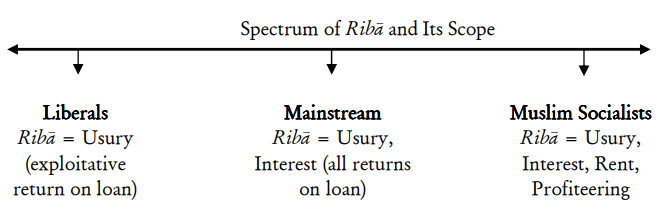
\includegraphics[width=0.9\textwidth]{CourantsIslamContemporain/ImagesCourantsIslamContemporain/Riba.png}

Rida part de l'analyse du mot \riba comme \textit{excès}, et en particulier reprend l'analyse de Co 3,125 présentée au début d'un excès lié à la renégociation de la dette. De là, il conclut que ce qui est interdit par le Coran sont les intérêts ajoutés à la fin de la période de prêt (\riba ’l-jahiliyyah). D'une certaine façon, ce sont les intérêts composés qui sont interdits, le fait que les intérêts augmentent en cas de non paiement. Cela lui permet d'autoriser les intérêts bancaires :
\begin{itemize}
    \item ils ne doublent pas les taux
    \item l'ajout d'un intérêt fait partie du principal de la même façon que le prix d'une vente à crédit (\emph{\riba al-buyu}) qui ne sépare pas principal et intérêt et qui est autorisé par le Coran.
\end{itemize}
 Il fait une distinction entre la \riba interdite dans le Coran et celle des Hadiths (voir graphique \ref{fig:MinorityRiba}) :

 \begin{figure}[h!]
     \centering
     \sidecaption{\cite{Siddique:DemystifyingRiba}, une séparation entre Coran et Hadith}
      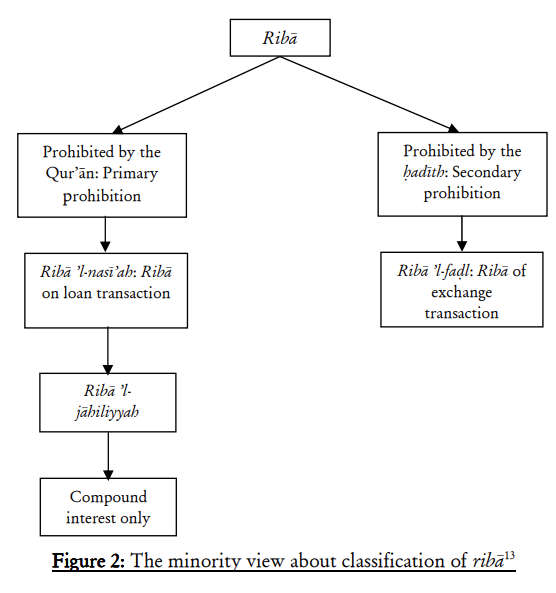
\includegraphics[width=0.5\textwidth]{CourantsIslamContemporain/ImagesCourantsIslamContemporain/RibaRida.png}
      \caption{La présentation du Riba selon Rida, dite minoritaire}
     \label{fig:MinorityRiba}
 \end{figure}
 
 Rida ne sera pas suivi par une majorités de jurisconsultes sur la légitimité des taux d'intérêt. En revanche, ils adopterons sa distinction entre less différents \riba, en étendant l'interdiction de la \riba du Coran à tout intérêt et pas seulement intérêt d'intérêt. Mais du coup, se pose la question du Hadith : pourquoi interdit-il  la \rib \emph{Al-Fadl}, c'est à dire la di
 
 

 
\paragraph{Les frères musulmans}
Dans les perspectives du réformisme musulman,
cette question d'ailleurs est loin d'être insoluble car une société qui émet des
actions peut être assimilée à une société en commandite. Les dividendes
représentent alors la part des bénéfices proportionnelle au capital engagé... 
al-Banna, fondateur des Frères Musulmans en Egypte, avait admis la licéité de ce
genre d'opérations et des Frères avaient, peu avant 1 948, fondé quelques ateliers
ou sociétés financées par ce procédé (2). La difficulté principale vient de ce que la
langue arabe n'a pas de mot spécial pour désigner les dividendes et que le terme
fâ'ida a des relents de ribâ.
\begin{quote}
    III. 2 interdiction de pratiquer l'usure, orienter les banques vers cette interdiction, le gouvernement doit donner l'exemple en abandonnant l'\textit{intérêt} fixé par les banque du prêt et du prêt industriel, etc. \textit{programme des frères Musulmans, 1936}
\end{quote}
%---------------------------------------------------------------------------------------------------------------
\section{Naissance de la finance et de l'assurance Islamique}

\subsection{Ce que l'on voit : Malaisie,...} 

\paragraph{une pratique supposant une \textit{shari'ah} qu'on ne peut interroger}

\subsection{Quelle est la théologie sous-jacente}

\paragraph{Une évolution de la shari'a par les principes} Mohammed Talbi 
\begin{quote}
    Il existe
trois principes en islam permettant de faire évoluer le droit et de
l'adapter
à la réalité, 

la \emph{maslaha} c'est-à-dire l'utilité publique, un
concept qui date du II\textsuperscript{e} siècle de l'hégire, 

la
\emph{zharoura}, la nécessité, c'est un principe fort puisqu'il est dit
que "la nécessité rend permis l'interdit" ; 

et les \emph{maqassid}, les
finalités de la loi. 

\begin{Synthesis}
On part des principes contre les principes. 
\end{Synthesis}
\sn{voir p. \pageref{TroisPrincipesEvolutionsShari}}
\end{quote}


\section{Conclusion}

\paragraph{une variété importante de vision mais toujours basée sur la sharia}

\paragraph{une réflexion sur la base de la Sharia'}
voir ce que Candiard dit de ce théologien qui dit de ne pas faire de Kalam mais du droit.

\paragraph{quel pourrait être les pistes de Kalam, quelques pistes de l'expérience occidentale ?}

\paragraph{St Thomas et l'usure : une réflexion autonome de la théologie}

\paragraph{extension du juste prix dans les risques : la dimension actuarielle}
\paragraph{Au XIXème, réflexion neo-thomiste et patristique pour sortir du carcan}
Après avoir regardé comment l'économie moderne, pensée au XVIIIème et XIXème questionne l'Islam à travers l'étude des différents courants de l'Islam contemporain, je poserai quelques pistes sur le propre questionnement du Christianisme. Après tout, le prêt à intérêt était aussi interdit au Moyen-äge en Europe. Ces pistes seront en particulier nourrie par l'étude de la pensée de Saint Thomas d'Aquin sur les taux d'intérêt et comment ces pistes peuvent nourrir la réflexion de la théologie musulmane. 

Nous catholiques au XIX par rapport à la modernité: renouveau thomiste et patristique. Liberté de pensée par rapport aux questions de l’époque
« A quoi on tient en vrai »
Le raccourci de certains théologiens musulmans : faire le court circuit pour repenser les choses : obsession juridique. Comment on sort du droit ? En faisant de la théologie. Et pour cela retour à la tradition
Voile
Le coran la dit donc il faut se voiler. Voile : hijab n’est pas dans le coran. Rideau
Zina : qu’il faut cacher
Jilbab pour les filles et femmes du prophète 
Ibn el jahouzi : voile non mentionné. Dimension non religieuse

Des écrits au XX. Deux raisons : les femmes vont occuper plus de rôle dans l’espace publique.
Et renouveau de l’anti théologie. Le voile est une question de théologie. Question de la foi
	⁃	Saint Paul : la foi et les œuvres
	⁃	On comprend croyant non pratiquant
	
\chapter{Matériaux bruts pour validation}

\section{A lire}
\href{https://www.persee.fr/doc/ridc_0035-3337\_1955\_num\_7\_3\_9521}{Le prêt à intérêt et l'usure au regard des législations antiques, de la morale catholique, du droit moderne et de la loi islamique }

\section{Refus de l'intérêt en milieu chrétien}

\subsection{1163 : le concile de Tours condamne le prêt à intérêt}


Le 01 septembre 2014

La condamnation du prêt à intérêt par l'Eglise n'a pas empêché, au travers de divers subterfuges, le développement du crédit, moteur de l'activité économique.

Dans l’Occident chrétien médiéval, le rôle de prêteur sur gages, souvent pour de faibles montants, sera longtemps assuré par des juifs, que leur religion autorise à prêter avec intérêt à des non-juifs. Mais dès le XIe siècle, de nombreux bourgeois chrétiens enrichis se livrent au prêt à une autre échelle. Déjà au XIIe siècle, des bourgeois d’Arras, de Cahors, des Lombards d’Asti, des Génois prospèrent par ces opérations.

Certes, l’Eglise et les princes qui se conforment à sa loi bannissent le prêt à intérêt en s’appuyant - entre autres - sur l’Evangile de Luc : "Prêtez-vous l’un à l’autre sans rien en attendre." En France, le concile de Tours de 1163 condamne une des formes du prêt à intérêt dans le cadre de la moralisation de l’Eglise : nul clerc (évêque, abbé) ne peut désormais prêter de l’argent et recevoir en gage un

\section{Extrait site internet}
\begin{quote}
En Islam, le Riba est interdit : il s’agit de l’un des plus grands péchés, qui tire son origine du Coran. Mais il est également l’un des plus banalisés. Le Riba, appelé « usure », désigne l’intérêt perçu sur de l’argent prêté. De nos jours, le Riba est partout présent dans le domaine financier, à savoir, dans les comptes d’épargne, dans les prêts à intérêts, dans les agios… Alors, qu’est-ce que le Riba exactement ? Pourquoi est-il interdit ? Comment financer vos projets sans Riba 
\paragraph{Définition du Riba}

Le Riba peut être défini par intérêt - usure. Si le terme « usure » est la traduction la plus fréquemment donnée à cette interdiction de l’intérêt usuraire, il est important de préciser que le mot Ribâ vient cependant du verbe rabâ \& arbâ qui signifie augmenter et faire accroître une chose à partir d’elle-même. 

Dans le contexte financier, il est donc interdit de réaliser des transactions financières basées sur du Riba. Or, lorsque vous possédez un compte courant conventionnel, l’argent qui y transite alimente un circuit basé essentiellement sur l’usure. En effet, dans ce contexte, la banque dispose de vos fonds afin de spéculer. Même principe lorsque vous êtes à découvert : les agios que vous devez payer vous impliquent dans la pratique de l’usure.

Mais ce n’est pas tout : lorsque vous épargnez votre argent sur des comptes de type livret Jeune, Livret A, ou PEL, les intérêts que vous touchez sont également basés sur la pratique du Riba, et cela que vous fassiez don ou non des intérêts.

Enfin, lorsque vous réalisez un prêt bancaire, vous participez au développement de l’usure en payant des intérêts. 

\paragraph{De nombreux versets du Coran interdisent la pratique de l’usure.}     En voici quelques-uns, qui sont particulièrement explicites :

Verset 130 de la Sourate 3, Al-Imran : « Ô les croyants ! Ne pratiquez pas l’usure en multipliant démesurément votre capital. »
Les versets 278 et 279 de la Sourate 2, Al-Baqarah : (V-278) « Ô les croyants, craignez Allah ; et renoncez au reliquat de l’intérêt usuraire, si vous êtes croyants. (V-279) Et si vous ne le faites pas, alors vous recevrez l’annonce d’une guerre de la part d’Allah et de son prophète. Et si vous vous repentez, vous aurez vos capitaux. Vous ne lèserez personne, et vous ne serez point lésés. »
D’après Abu Hurayra, le Prophète (SAWS) a dit : « Evitez les 7 turpitudes ». Lorsque les compagnons demandèrent : « Quelles sont-elles, Ô envoyé d’Allah ? », il mentionna l’usure aux côtés notamment du polythéisme, du meurtre…
D’après Sahih Muslim : Ubâdah Ibn As-Sâmit rapporte que le Messager d’Allah (SAWS) a dit : « Or pour Or, argent pour argent, blé pour blé, orge pour orge, datte pour datte, sel pour sel, de manière égale, de main en main. Si la nature des produits diffère, vendez comme vous le voulez, si c’est de main en main ». \sn{\href{https://firstunion.fr/quest-ce-que-le-riba/}{First Union} ? }
\end{quote}

 
 \paragraph{Abd ar-Rahman ibn Nasir as-Sadi}\href{https://fr.wikipedia.org/wiki/Abd_ar-Rahman_ibn_Nasir_as-Sadi}{Abd ar-Rahman ibn Nasir as-Sadi} Oulema Hanbalite saoudien 1889. influencé par 	
Ibn Taymiyya
Mohammed ibn Abdel Wahhab
 
 \paragraph{ Le ribâ (l’usure) dans l’Islam}
 
 \href{https://www.ajib.fr/le-riba-lusure-dans-lislam/}{Le riba est l'usure dans l'Islam}
 
 \begin{quote}
    


Pour comprendre le sens réel du ribâ, pour connaître son statut légal dans l’islâm, houkm, qui est bien sûr, l’interdiction, ainsi que les méfaits individuels et collectifs qu’il engendre, il faut comprendre quelques points importants.

Parcourons ensemble ces extraite du livre « Le résumé des vertus de la religion musulmane » du grand savant \textit{Abdarrahman As-Sacdî} qui nous éclaireront sur la vue de la législation islamique, \emph{shariah}, sur les transactions, licites et illicites, ainsi que la sagesse du Législateur, Allah, soubhânah, en établissant cette auguste législation.

Nous verrons en particulier, les problèmes qui concernent le ribâ.

\begin{quote}
    
Que signifie le ribâ ?

Le ribâ signifie l’usure. Si l’on entend par « usure » le prêt à taux supérieur à zéro.

Car la définition contemporaine de « l’usure » est « l’intérêt excessif » ou « l’intérêt supérieur au taux légal », tandis que le ribâ est le prêt à intérêt, aussi minime soit-il.

Le prêt islamique légal est donc le prêt à zéro intérêt. Et le ribâ est l’usure dont l’intérêt est supérieur à zéro.

Il y a plusieurs types de Ribâ :
\begin{itemize}
    \item 1/Le prêt à intérêt : le surplus, aussi minime soit-il, perçu, pour le prêt, par le créancier en échange du délai accordé.

 \item 2/Ribâ al-fadhl : le surplus perçu lors de l’échange d’un bien ribawî (relatif au ribâ) tel que l’échange de l’or avec l’or, de l’argent avec l’argent, du blé avec le blé… etc.

 \item 3/Ribâ an-nasî’ah : différer l’encaissement lors d’un échange d’un bien ribawî de même nature, tel que l’or avec l’or, ou de nature différente, mais dont la cause ribawique est commune, tel que l’or avec l’argent.
\end{itemize}


\paragraph{Quelles sont les transactions dites légales dans le \emph{shariah}, halal ?}

La vente rendue licite par la législation islamique ainsi que le louage[1], les sociétés et les différentes transactions ; celles où s’échangent les marchandises entre les gens, les dettes, les utilités… etc.

\paragraph{Pourquoi une transaction est légale dans le \emph{shariah}, dite : halal ?}

La législation parfaite a permis ce type de transaction et l’a autorisé aux hommes, car cela assure leurs intérêts – nécessaires, indispensables ou complémentaires -.

Elle a élargi ainsi considérablement la liberté des hommes afin que leurs affaires et leurs conditions se réforment et que leurs vies s’ordonnent.

Quelles sont les conditions de la légalité d’une transaction ?

\textbf{La législation, \emph{shariah}, posa comme conditions pour que les transactions soient licites :}

1-La satisfaction des deux parties ;

2-la clarté du contrat ;

3-la connaissance de l’objet du contrat, de la durée du contrat et des conditions qui en résultent.



Quelles sont les transactions interdites dans la \emph{shariah}, dites : haram ?

La législation, \emph{shariah}, a interdit tout ce qui comporte un préjudice ou une injustice tel que :

1-Les différents types de jeu de hasard,

2-le Ribâ ;

3- l’ignorance[2], la jahâlah.
\end{quote}
 

Cette division, licite et illicite, halal et haram, prescrite par Allah et révélée à Son Prophète Mouhammed, ainsi qu’à tous les Prophètes avant lui, a pour objectif essentiel de préserver le but premier escompté par ces opérations d’échange entre les humains : l’intérêt mutuel, l’avantage commun à toutes les parties de l’échange et le bénéfice pour tous.

Inversement, tout ce qui n’apporte pas d’intérêt commun et ne fait pas bénéficier toutes les parties qui opèrent la transaction est illicite, haram et interdit.

Car cela va à l’encontre de la raison de cette opération d’échange, la transaction, qui est l’intérêt commun et l’absence de préjudice.

\textbf{Le ribâ fait partie de cette catégorie car son intérêt va dans un sens unique, qui est celui de l’enrichissement du créancier, et il porte un préjudice considérable au débiteur.}

Ceci s’appelle : injustice, iniquité et celui qui en profite ne fait que manger l’argent et les biens des autres injustement.
 \end{quote}
 
 
 \paragraph{Dictionnaire du Qoran}
 

 \section{Demystifying Riba through the Methodology of Muslim Jurists}
 \href{https://www.proquest.com/docview/2352353188?accountid=143046&parentSessionId=Sg7rHgjzHS0M9aF4pv1Nx2pxOOyR5LkKvILKrOVqG1o\%3D&pq-origsite=summon}{Demystifying Riba through the Methodology of Muslim Jurists}\sn{MUHAMMAD ZAHID SIDDIQUE; MUHAMMAD MUSHTAQ AHMAD.
Islamic Studies; Islamabad Vol. 58, N° 2,  (Jun 30, 2019): 169.}
 \cite{Siddique:DemystifyingRiba}



 \subparagraph{Summary}
  \begin{quote}
  In the post-colonial world when Muslims tried to restructure their public life in accordance with the shari‘ah, they developed a new discipline known as Islamic economics one of the central constructs of which is prohibition of riba. Unfortunately, the discussion among modern academic circles assumed a wrong methodology, which resulted in mystification of this concept and, hence, in a number of unsettling questions. This paper explains the nature of the mistake committed by modern Muslim scholars and economists. It also outlines the structure of correct methodology, which was laid down by premodern Muslim jurists for understanding the concept of riba and all other legal terms. The paper develops a consistent analytical framework for addressing majority of the questions on the subject of riba and attempts to rectify the mystification created around this concept.
  
  \end{quote}
 \subparagraph{Texte intégral}
 \begin{quote}

Keywords: riba, interest, loan, bay‘, Islamic economics, Islamic legal theory, financial regulations of Islam.

1. Introduction

After losing their political rule to the imperial powers, Muslim societies faced the widespread dominance of interest-based banking system. According to the majority of Muslim scholars and jurists, bank interest (riba) was not allowed, but Muslim societies got engaged in it due to growing spread of interest-based banking in modern societies and the non-availability of interest-free banking. \mn{noter aussi que le développement de la banque s'est fait en parallèle dans les sociétés occidentale. }

Muslim scholars and economists demanded its alternative soon after Muslims got independence from their foreign masters. Commitment to follow religious teachings in the public affairs of life and liberty from the colonial oppressors provided the required room, which resulted in what is now known as Islamic economics in general and Islamic finance/banking in particular.

One of the central concepts of Islamic banking is prohibition of riba, which unfortunately and surprisingly remained controversial among Muslim economists and scholars. Different perspectives about the meaning of riba prevailed in the twentieth century. Majority view holds that both usury and bank interest are equally impermissible in Islam while business profit is allowed.\footnote{1 For  detailed  arguments  of  this  position,  see  Ab┴ ’l-A‘la  Maud┴di,  S┴d  (Lahore:  Islamic Publications,  2000),  110–12;  M.  Umer  Chapra,  “The  Nature  of  Riba  in  Islam,”  Hamdard Islamicus  7, no.  1 (1984):  3–24;  Muhammad  Shafi‘, Mas’alah-i  S┴d  (Karachi: Idarat  al-Ma‘arif, 1996), 43–47; Muhammad Ayub, “What  is Riba? A  Rejoinder” Journal of Islamic  Banking and Finance  13,  no.  1 (1996):  7–24;  Muhammad  Taqi Usmani,  The  Historic  Judgment  on Interest Delivered in the Supreme Court of Pakistan (Karachi: Idarat al-Ma‘arif, 1999), 12–16; Mohammad Nejatullah  Siddiqi,  Riba,  Bank  Interest  and  the  Rationale  of  Its  Prohibition  (Jeddah:  Islamic Research  and  Training  Institute, 2004),  45–48;  and  Mahmoud A.  El-Gamal,  Islamic  Finance: Law,  Economics,  and Practice  (Cambridge:  Cambridge University  Press, 2006),  46–52. Within this  category,  there  are  further  two  approaches.  One  approach  that  represents  traditional ‘ulama’ emphasises the resurgence  of only those business contracts that were approved by  the early  Muslim  jurists.  It proposes  profit-and-loss  sharing (PLS)  as an  ideal alternative  to riba. Though it does not deny the permissibility of other than PLS-based financing instruments such as murabahah and ijarah, yet it affirms that equity-based financing method is the primary means of achieving desirable economic objectives. The second approach is pragmatic one. It justifies a more liberal and flexible stance on structuring shari‘ah-compatible transaction forms that looks for financial engineering to meet all demands of modern banking customer.  }

Contrary to the majority view, some modern Muslim scholars dispute that the Qur'anic term riba includes interest paid and charged in the banking system.\footnote{ Muhammad Rashid Rida (d. 1935) was among the foremost proponents of this theory. See his al-Riba  wa ’l-Mu‘amalat  fi ’l-Islam  (Cairo: Dar  al-Manar, 2007).  Also see  Sayyid  Yaqub Shah, “Islam  and Productive  Credit,” The  Islamic  Review  47,  no.  3 (1959):  34–37; Fazlur  Rahman, “Riba  and  Interest,”  Islamic Studies  3, no.  1 (1964):  1–43; Timur  Kuran, “On  the Notion  of Economic  Justice  in  Contemporary  Islamic  Thought,”  International  Journal  of  Middle  East Studies  21,  no. 2 (1989): 171–91;  Izzud-Din Pal,  “Pakistan and  the Question  of Riba,”  Middle Eastern Studies 30, no. 1 (1994): 64–78; and ‘Abd al-Karim Athari, S┴d Kiya Hay? (Mandi Baha’ al-Din: Anjuman-i Isha‘at-i Islam, 2008), 8–12}
To them, replacing bank interest with anything else is tantamount to obstructing natural operation of economy and creating inefficiencies because interest is the just reward of capital reflecting its marginal productivity. \sn{ Constant  J.  Mews  and  Ibrahim  Abraham,  “Usury  and  Just  Compensation:  Religious  and Financial Ethics in Historical Perspective,” Journal of Business Ethics 72, no. 1 (2007): 1–15}

3 According to this perspective, there is no need to have anything distinct like “Islamic banking” to begin with because the existing system is already Islamic.


Finally, on the other extreme are \textit{Muslim socialists}\sn{A l'autre extrême ?} who develop their version of Islamic economics based on socialist policy package.\sn{See Ghul┐m A╒mad Parvaiz, Ni╘┐m-i Rub┴biyyat (Lahore: Id┐ra-i ║ul┴‘-i Isl┐m, 1978). }

 Since socialism considers wage as the only legitimate reward of a factor input, the scope of riba is much wider than usury and bank interest according to these scholars. 

It is believed by some\sn{Raf┘‘ All┐h Shih┐b, Kir┐yah-i Mak┐n┐t k┘ Shar‘┘ ╓aithiyyat (Lahore: Kit┐b Ghar, 1981)} that rental earnings on an asset is also included in riba because rent is similar to interest earnings as both are the prices of capital determined by similar market forces. Others are of the view that not only bank interest but also trade or merchant profit is banned under the category of riba.


6 They argue that as lender is forbidden the right to charge interest from poor borrower, so should be the rich industrialists and landlords from appropriating lion's share of value-added on the name of profits.

They assert that loaning riba (riba 'l-qard) covers money lenders and hoarders who charge against time while riba of excess (riba 'l-fadl) is the domain of landlords, merchants, and middlemen who exploit poor workers and make unequal exchanges. 

These differing perspectives are shown in figure 1. Because this last perspective about riba has gained very little popularity among Muslim scholars and masses as compared to the first two, we exclude its analysis from the scope of this paper, though it would be analysed indirectly.


Spectrum of Riba and Its Scope Liberals Mainstream Muslim Socialists Riba = Usury Riba = Usury, Riba = Usury, (exploitative Interest (all returns Interest, Rent, return on loan) on loan) Profiteering


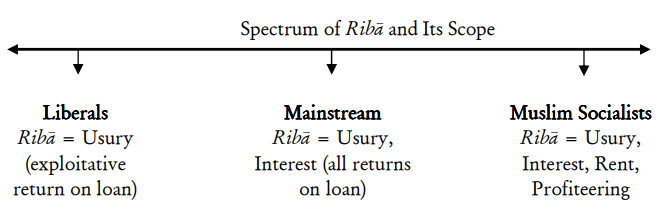
\includegraphics[width=\textwidth]{CourantsIslamContemporain/ImagesCourantsIslamContemporain/Riba.png}



The above differences have left scholars divided on several important questions that demand straightforward answers. Those questions include the following ones:
\begin{itemize}
    \item 
1. Is bank interest prohibited in the light of the Qur'an and the sunnah? If yes, how?
    \item 
2. Whether the Qur'anic term riba includes all kinds of interest rates or it relates only to the excessive interest rates?
    \item 
3. Whether the scope of riba extends to the interest charged and paid on business transactions in the banking system or is restricted to the interest charged on consumption loans only?
    \item 
4. Does Islam allow loan transactions? If yes, how and in what form?
    \item 
5. Is paying interest a lesser evil as compared to charging it?
    \item 
6. Is borrower always \textit{mazlum} (a losing party) in an interest bearing loan transaction?
    \item 
7. Does Islam allow indexation of loans on the grounds of inflation?
    \item 
8. Is credit-sale with higher deferred price as compared to the spot price allowed?
    \item 
9. Does Islam approve of “time value of money,” especially when charging higher deferred price is allowed in a credit sale?
    \item 
10. Are future currency contracts permissible in Islam?
    \item 
11. How and to what extent is salam transaction permissible?
\end{itemize}


These are but a few questions.
\begin{Synthesis}
We show in this paper that whatever confusion prevails among contemporary scholars on this subject is the outcome of following an inadequate methodology for determining the meaning and scope of riba.
\end{Synthesis}
 In fact, this methodology has mystified the nature of riba, which is otherwise clear when viewed from the methodological view point of the eminent Muslim jurists of the past. The mystification is such that not only it results in confusing answers to these questions but it also begets confusing questions. Unfortunately, the confusion has built up to the extent that the Federal Shariat Court of Pakistan has been struggling to come up with a definition of riba. It is in this background that this paper attempts to explain:

(1) the contemporary Islamic economists' methodology of interpreting and classifying riba; (2) why this methodology is wrong and insufficient; (3) the methodology of understanding riba on the pattern of Muslim jurists of the past; (4) that the methodology given by the Muslim jurists is coherent and compact.

The reader will encounter a number of arguments in this paper that are advanced by those who justify bank interest. Since the paper deals with the legal substance and not with the economic merits of arguments, hence we will restrict ourselves to the legal analysis of those arguments and leave aside their economic analysis and rationale, which require an altogether different methodology. Any legal system has three aspects: (1) what: the legal rulings (i.e., ahkam); (2) how: the rules of deriving those legal rulings (i.e., usul al-fiqh); and (3) why: the underlying rationale(s) and wisdom behind the legal rulings (i.e., hikmah)

It is important not to mix these aspects. The present study deals with the first two aspects of the issue of riba. Moreover, the classification of riba discussed in this paper is primarily based on the methodology of Hanafi jurists for ensuring analytical consistency. We presume that a school of law represents an internally coherent system of interpretation and that mixing up the views of the various schools results in inconsistencies.7 However, views of the other schools have been briefly mentioned in the footnotes wherever required. Finally, the paper does not attempt to show that the Hanafi jurists' approach is superior to all others, rather it explains that the classical jurists' approach (whether Hanafi, Maliki, Shafi‘i or Hanbali) to understanding riba is superior to that of the modern scholars. The methodology of these jurists share several common results that are important in order to answer the above questions.

Following section outlines the method adopted by modern Muslim scholars and economists. The next section discusses problems in this methodology and develops the skeleton for the methodology that is then applied in the coming section, which details out the general rules of riba alongside their resulting implications. The last section concludes the paper by giving a comprehensive definition of riba based on discussions in sections three and four.


\newpage
\subsection{Outline of the Mystifying Methodology}

Imran Ahsan Khan Nyazee\sn{\href{https://en.wikipedia.org/wiki/Imran_Ahsan_Khan_Nyazee}{Pakistan} Nyazee's academic career was inspired by the work of Abdur Rahim. Nyazee argues firstly, that due to its unique set of principles of interpretation, each school of Islamic law represents a theory of law unto itself. Secondly, he points out that Istiḥsān cannot be understood without understanding of the workings of qiyās. It is, therefore, difficult to accept that there was no system of interpretation before al-Shāfi‘ī's time. Thirdly, he concludes that the uṣūl al-fiqh never existed. Furthermore, Nyazee describes beyond the individual fikh of each school of law, another theory of interpretation called maqāṣid al-sharī‘ah (theory for the purpose of the sharī‘ah) which was developed by al-Ghazālī. Nyazee has written and self-published on a number of aspects of Islamic law. He agrees with most Muslim scholars that strictly speaking, selling money (taking interest) is prohibited, according to Islamic law. Some point out a difference between the treatment of riba in the Qur'an versus the Sunnah but Nyazee the two approaches are actually one and the same.Nyazee also proposes that all loans (except those of a charitable nature without a fixed period of repayment) and therefore all banking is prohibited and unIslamic. Nyazee is equally intolerant of murabaha, the Islamic system of business where in-put costs and mark-ups are made transparent between vendor and buyer. He argues riba will inevitably enter such transactions.[10] He extends the prohibition to the creation of wealth on the basis of debt and the fractional reserve banking system. These elements along with zakat (the system of alms-giving) he says, are the differences between Islam and capitalism. He advocates the use of the gold and silver dinars and dirhams as the currency of the Muslim community. Nyazee would also prohibit the corporation or 'legal personality' under Islamic law.} explains that the methodology adopted by modern scholars for determining the meaning of riba is the same, though they disagree in their conclusion regarding whether or not bank interest is riba.8 The fundamental problem of their methodology lies in overlooking the inherent link between the Qur'an and sunnah. This methodology of interpreting riba was initiated by Muhammad Rashid Rida (d. 1935) \sn{voir p. \pageref{Theol:Rida} Frère musulman pas le voyage en Europe. Plue el manar un commentaire coranique, sensé être l'héritage d'abdu}, which goes as follows:9

\paragraph{Lecture de Rida El Manar}
Riba is classified into two categories, riba of the Qur'an (also equated with riba 'l-nasi'ah, i.e., interest on loan transaction) and riba of hadith (equated with riba 'l-fadl, i.e., interest on exchange transaction).

Rida begins with literal meaning of the word riba (excess) and then traces some riba-based transactions practiced by Arabs during the time of Prophet (peace be on him). Rida, relying on some commentators of the Qur'an, asserts that the Qur'anic verse regarding riba deals with a specific practice of Arabs known as credit-sale where the payment of price is deferred to a future period while delivery of goods takes place on spot. Because a seller is allowed to charge whatever price he wants in a sale transaction, no riba is involved in the original price negotiated between the two parties-any excess in future price becomes part of the price. However, they used to increase the price excessively whenever the debtor would be unable to settle his debt obligations at the end of payment period. The debtor was given the option, “Will you pay the debt or increase the amount in lieu of delay?”

For Rida, it was this excessive rate (doubling and multiplying) of interest in debt-based transactions added to the original sum at the end of payment period which was prohibited by the Qur'an (he called it riba 'l-jahiliyyah).10 From this, he concluded that the bank interest is not the same riba that was deemed impermissible by the Qur'an because (a) it is neither doubling and redoubling of rates (b) nor the excess is stipulated in the initial period of the banking transaction-he assumes that the initially added interest is part of the principal or original sum just like the original sum in case of credit-sale. 
\begin{Synthesis}
Hence, for Rida, only compound interest is prohibited.
\end{Synthesis} 

Other scholars, supporting Rida's view, added that business loans were not common among Arabs as theirs was a subsistence economy; loans were largely taken by poor people for consumption purposes on interest and whenever they were unable to repay them at due time, excessive interests were added to the original sum. Hence, it was this type of interest that was declared prohibited by the Qur'an and it has nothing to do with the modern commercial loans, \textbf{which are mutually beneficial for both parties.}11

Having ascribed this meaning to the Qur'anic word riba on the basis of some historical traces, Rida then explains the form of riba declared impermissible in the sunnah as a distinct prohibition from that of the Qur'an.
\begin{Def}[Riba] Usure, profit ou gain réalisé sur un prêt.
\end{Def}

\begin{Def}
[Riba al-buyu] : Usure. Opération de vente dans laquelle une matière première est échangée contre la même matière première mais en quantité différente et la livraison d’une des matières premières est postposée. Pour éviter le riba al-buyu, les matières premières échangées par les deux parties devraient être en quantités égales et l’échange devrait être instantané. Riba al-buyua a été condamné par le Prophète Muhammad afin d’éviter que le riba (intérêt) n’affecte insidieusement l’économie.
\end{Def}
\begin{Def}[Riba al-duyun] : Usure d’une dette.
\end{Def}
 
\begin{Def}[Riba al-fadl] : La différence de quantité entre deux biens échangés et comportant du riba.
\end{Def}
\begin{Def}[Riba al-nasiah] : La différence de paiement liée au report de deux biens comportant du riba
\end{Def}\mn{cf Glossaire des termes financiers  Islamiques \href{https://www.cairn.info/la-banque-et-la-finance-islamiques--9782804167042.htm}{Banque et finance islamique} } He calls it \textit{riba 'l-fadl} which emerges in the exchange of two counter values of the same or different species and hence also called \textit{riba 'l-buyu‘}.12 The position of Rida, which may be termed as minority view, is summarised in figure 2.


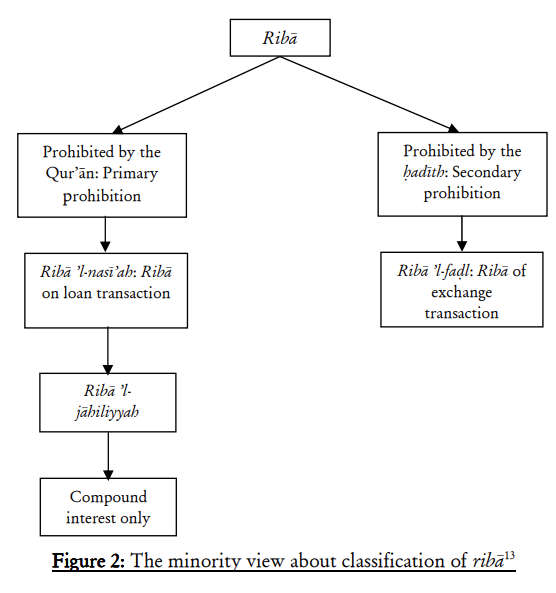
\includegraphics[width=\textwidth]{CourantsIslamContemporain/ImagesCourantsIslamContemporain/RibaRida.png}

Thus, Rida dichotomised the two concepts of riba, one attributed to the Qur'an and another to the sunnah. He finally declared the first one as real or explicit riba while latter as lighter or implicit riba.
\textbf{
Though the majority of contemporary scholars did not agree with the conclusion drawn by Rida about legitimacy of bank interest, however they adopted his methodology of classifying riba. The only difference in their opinion is that riba of the Qur'an includes all rates of return on loan and it is not merely restricted to the compound interest of jahiliyyah}\sn{la période pre islamique}


To them, business loans were a part of Arab's economy and any contractual return to lender is unfair because this is tantamount to refusing to share business risk with the borrower. We can depict their views in figure three.
\begin{Synthesis}
On a donc un nouveau problème, le pret commercial lié avec l'industrie et face à ce nouveau problème, une lecture de Rida qui est assez positive (Riba = Excess) mais qui note une différence entre Coran et Sunna) et fait une distinction entre les deux, reprises ensuite par les autres légistes, mais en repartant d'une lecture stricte du Riba comme intérêt. Il conveint d'articulier Coran et Sunna de façon non parallèle mais l'un par l'autre.
Il convient de montrer l'évolution du prêt commercial au XIX
\end{Synthesis}
Because the sunnah is not linked with the Qur'an in this methodology, both the minority and majority Muslim economists have struggled to explain as to why someone would engage in exchange transactions of the forms mentioned in hadith. Some opined that these transactions are declared impermissible because they may open the path for the “real riba” (i.e., riba of the Qur'an).


14 Others assumed that it was meant to discourage the practice of barter exchange and promote market exchange through a medium of exchange.15 Yet another view argues that it eliminates the possibility of benefiting from asymmetric information of the contracting parties.16 The truth is that none of these explanations makes the point.

2.1. The Nature of Debate within Minority and Majority Schools

The debate that has taken place within the followers of this mystifying methodology on the issue of why or why not bank interest is riba may briefly be summarised here. As explained above, Rida asserted that bank interest was not included in the Qur'anic concept of riba of debt because it was different from the riba that was charged by Arabs on credit-sale transaction by doubling and multiplying the price whenever the debtor was unable to settle his debt at due time and asked for relaxation in payment period.18 Rida explained that the Qur'anic verse “Allah has permitted bay‘ and prohibited riba”19 referred to this riba. To strengthen his case, he argued from the verse: “O Believers! Do not devour riba doubled and multiplied and fear God so that you may prosper.”20

This verse complements the former verse in the sense that what was implicit in the first verse was made explicit in the latter-both verses referred to the practice of doubling and multiplying of interest and none of them forbad the bank interest.

How do the majority of scholars respond to this argument? For example Usmani notes the Qur'anic verse:

O you believers! Fear God and give up riba that remains outstanding if you are true believers. Behold! If you do not obey this commandment, then God declares war against you from Himself and from His Prophet. But, if you repent (from riba), then you are entitled to only your principal amounts. Neither should you inflict harm to others, nor others should do harm to you.21

The argument is based on the emphasised words ‘you are entitled to only your principal amounts (ra's al-mal)'. He infers from these words that the rightful entitlement of lenders is the original sum advanced; he cannot charge any increase whether small or large (doubled and tripled). To him, the verse (3:130) forbids a severe form of riba where interest is multiplied, but it does not restrict riba to this specific form. Hence, bank interest falls within the purview of the Qur'anic verse “Allah has permitted bay‘ and prohibited riba.”22 They are also of the view that charging interest on commercial loans was also practiced by Arabs.23

Does the above analysis of mainstream scholars guarantee the prohibition of bank interest? We are afraid it does not. Their arguments rest on two assumptions:

(1) The verses (2:278-79) address the issue of loan-transaction.

(2) Ra's al-mal (principal amount) can only refer to the original principal advanced in loan.

Both of these assumptions are problematic. Following submissions can be made against them:

(a) If the meaning of the verse is to be determined with reference to historical practices, one can equally claim, just like Rida, that the verse is not about loan transaction but about credit sale. In that case, ra's al-mal is not referring to the principal amount lent; rather, it is the deferred future price of the goods sold. On which legal grounds or facts can this claim be dismissed?

(b) Further, this deferred price might include increase over and above spot price. Hence, the future price could consist of two components: spot price plus some additional profit. The sum of these two would constitute ra's al-mal (principal amount) in this transaction (i.e., principal amount in credit sale (ra's al-mal) = spot price + extra profit)

Whenever a debtor was unable to repay full amount, further multiplied increase was added to this original sum, Rida called it interest. This would increase the due amount to: total amount after increase added due to delay, which is interest in addition to ra's al-mal.

Using this structure, one can then argue that the initially added interest in a loan transaction is equivalent to initially added “extra profit,” which becomes part of ra's al-mal. Therefore, entitlement to the ra's al-mal means entitlement to the simple interest, as claimed by Rida.

(a) The only legal justification for ascertaining that the verse is about loan transaction is based on the words “ra's al-mal” (principal amount). But how can it be settled that ra's al-mal here means ra's al-mal of a loan transaction? This question is important because a number of transactions constitute a component of ra's al-mal. For example, there is ra's al-mal both in mudarabah and musharakah contracts. How to exclude these forms of ra's al-mal from the purview of the Qur'anic verse? If someone says, “This verse is about loan, so ra's al-mal refers to that of loan contract and not of mudarabah and musharakah,” he is clearly arguing in circularity. The argument goes like this:

Q: How do we know that the verse is about loan contract?

A: Because the verse talks about ra's al-mal.

Q: How do we know that ra's al-mal here refers to that of loan?

A: Because the verse is about loan contract!

A circular argument is no argument.

(b) Muslim Socialists could maintain that ra's al-mal means principal amount of all business contracts. Therefore, it is not legitimate to charge any excess over and above principal amount, no matter it is mudarabah, musharakah or ijarah.

Not only that the analysis of mainstream scholars does not necessarily imply the prohibition of bank interest, it leads to a set of unsettling arguments that have left Islamic economists bewildering about some basic issues. For example,

(1) Even if it is agreed that ra's al-mal means principal amount of a loan transaction, does it mean “nominal” amount or the “real” (inflation adjusted) amount? Again, what are the legal grounds to settle this issue? Because there are no clear-cut legal grounds available in this methodology, we see scholars are divided on this subject matter-some allow indexation of loan against inflations while others do not.

(2) What about the question of “time value of money?” This question poses challenge for Islamic economists because they, as a rule, approve the practice of charging higher price in credit-sale and murabahah.

(3) The Lawgiver has allowed salam, what are the legal grounds for not extending this permission to currency salam (future currency contracts)?

Undoubtedly, majority view has addressed these issues, but the answers do not seem to be stemming out of a coherent analytical legal system. This approach is often found mixing up legal analysis with economic analysis. This missing coherent analytical legal system is the root cause of most of the mystification that has prevailed all over. It is an unfortunate state of affairs and it is high time to demystify things.

3. Methodological Assumptions of Premodern Muslim Jurists (Fuqaha') for Understanding Riba

To understand the method used by the eminent premodern Muslim jurists for understanding riba, three methodological issues (MI) need to be clarified. They are explained by Nyazee in detail.24

1) Link between the Qur'an and Sunnah

The methodology adopted by the modern Muslim scholars and economists is misleading because it delinks the Qur'an and sunnah. It assumes that the meaning of riba is different in the Qur'an and sunnah, which is not the case. To explain the nature of error made by both the groups, it should be noted that Muslim jurists (fuqaha') classified riba in the category known as mujmal (unelaborated)25 whose meaning and scope cannot be determined without explanation (bayan) of the Lawgiver (Shari‘). The famous hadith (as given in footnote 1) that explains different usurious transactions actually does not add something to the Qur'anic word riba. Rather, it defines its meaning and scope.

Thus, while to the contemporary scholars the meaning of riba is known independent of hadith and they see hadith as adding some more cases to the Qur'anic concept of riba, the jurists say that hadith is the definition of the term riba used by the Qur'an. Thus, riba 'l-nasi'ah and riba 'l-fadl both are included in the Qur'anic concept of riba.

2) Relationship between Loan and Bay‘ (Exchange)

Loan is also classified as a form of exchange transaction (bay‘)26 by Muslim jurists. The scope of this paper does not allow detailed analysis of this assertion.27 For descriptive purposes, it can be seen that a loan of Rs X is an exchange of Rs X today with Rs X after time deferment (and with Rs X + Y if interest payment of Rs Y is included). Figure 4 depicts this nature of loan transaction by illustrating a loan transaction between Mr. A and B:

3) Skeleton of a Coherent Legal System

A coherent shari‘ah-based legal system consists of a set of general rules, called

‘azimah by the jurists, supplemented by some exemptions to these laws, called rukhsah. In the words of Nyazee, ‘Azimah (lit. determination, resolution) is applied to mean a rule that is applied initially and for itself. Such rules form the backbone of the law. As against this, there may be a rule that goes contrary to the requirements of the initial rule, but is permitted by the law. This rule is considered to be a rukhsah (exemption) from the initial rule.28

This classification of ‘azimah (the higher or first order rules) and rukhsah (the lower or second order rules) is important for several reasons.

First, it explains the order in which the rules have to be applied.

Second, it explains why sometimes two opposing cases may be allowed within a given skeleton of law.

Third, the order of rules implies that an exception cannot be extended using any method of argument, whether analytical or analogical. On the other hand, extension of first order rules is legitimate by these methods. In other words, it is not allowed to build a sub-legal system based on exemptions because otherwise it starts negating the primary provisions and objectives of the law-an exemption from the general rule must remain an exemption.

Fourth, because of the logical hierarchy in the operations of ‘azimah and rukhsah, it is clear that an exemption from a rule cannot be used to nullify or change the shari‘ah status (hukm) of any other case that is derived from the general rules. Alternatively put, an exemption (a lower order rule) cannot prevail over the higher order rules.

Fifth, because all rules and exemptions are derived from nusus (the Qur'an and sunnah), hence the only justifiable exemptions are the ones, which are given in nusus (i.e., stated by the Lawgiver Himself).

We call these nusus the “facts” of the shari‘ah-based legal system in this paper. Given these “legal facts,” the task of a jurist is to derive those general rules (‘azimah) from the facts, which render these facts internally consistent and extendible on the one hand and highlight the exemptions (rukhsah), if any, on the other.29 Finally, the general rules and exemptions generate some implications, called ahkam. This skeleton of a shari‘ah-based legal system is illustrated in Figure 5. We apply this skeleton in this paper to elaborate riba.

The relevant “legal facts” used by premodern Muslim jurists to derive general rules and exemptions are quoted at the relevant places in this article. We are now in a position to take on the issue of derivation of the general rules and the implications from those “facts.”

4. Underlying Rules behind the System of Bay‘ in Jurists' Methodology

Our intention in this paper is to reveal that the apparently large and complicated system of legal injunctions (ahkam) is reducible to a few set of rules derived from fewer legal facts. We propose that a majority of ahkam (legal injunctions or provisions) governing economic transactions (buyu‘) can be derived from three broad rules:

1. Rules of riba mentioned in the sunnah. This is not a single rule, rather a set of rules as explained below.

2. Rule about the sale of goods not possessed by a person.

3. Rule about exemption that an exemption is to be treated as exemption.

Before explaining these rules, we first explain the context of the Qur'anic verses that underlies the jurists' methodology of riba to clarify the misconception that the relevant verses of Surat al-Baqarah are about loan transaction and not exchange (bay‘).

4.1. The Context of the Verses of Surat al-Baqarah

The Qur'an states that the disbelievers said, “Verily, bay‘ (sale) is just like riba.” In response to this, it was said, “Allah has permitted bay‘ and prohibited riba.” To understand why the disbelievers said this, consider these three transactions:

(a) A gives B 100 grams of gold in exchange of 110 grams of gold to be paid after one year. This is primarily a sale contract as explained previously (i.e., exchange of 100 grams gold with 110 grams gold with time lag) and involves riba (how, this will be explained in the next section but take it for granted for the moment).

(b) A asks B for 100 grams of gold in exchange of, say, 500 kg wheat at spot. This is a legitimate regular sale contract.

(c) A demands from B 110 grams of gold in exchange of 500 kg wheat for payment of price after one year: this is credit sale contract with higher deferred price as compared to spot price and is also legitimate (this is explained in section 4.3).

The credit sale was a common practice among Arabs and, therefore, they were confused as to why the transaction (a) is impermissible and (c) is permissible while the two are quite similar in nature (i.e., both are credit sales and both involve access payment). In (a), 10 grams of additional gold are paid as counter-value for 100 grams of gold for a delay of one year and similarly 10 grams of gold are paid for a delay of one year in transaction (c). It is for this reason that disbelievers said, “Verily sale is just like riba!” That is, transaction (c) (i.e., the credit sale) is similar to the transaction (a). The technical reason for allowing transaction (c) and forbidding (a) is the similarity of genus which is explained by the sunnah. This is explained in the next sections in detail, but the important point to note here is that the assumption that the Qur'anic term riba is not about sale contract, rather it is about debt, is not implied by these verses.

Thus, the verse says that Allah has approved all forms of buyu‘ (exchange transactions) except those which involve riba.30 The natural question then arises: what is this thing called riba? Has the Qur'an given any definitive description of riba?

One may make one of the two assumptions here. First, the concept of riba was largely a sort of common knowledge for everyone and, hence, it required no legal description by the Qur'an. That common knowledge is traceable by an examination of historical record of Arabs which provides sufficient legal foundations for determining the meaning of riba. As far as the details of riba in the sunnah are concerned, they were additions over and above to that common knowledge of riba and most of these additions were unknown to the Arabs. The liberals and mainstream scholars share this assumption and we believe that this assumption constitutes what we called the “mystifying methodology.”

Second, some forms of riba may be or actually known to the Arabs but these do not set the legal standard against which the Qur'anic concept of riba is to be determined. As it is a legal term, its meaning has to be sought from the Lawgiver. In technical sense, the jurists call it mujmal (unelaborated) for which elaboration (bayan) is sought from the Lawgiver. This elaboration of the legal meaning of the Qur'anic term riba is given by the sunnah. After this elaboration by the Lawgiver, its meaning is determined definitively and it becomes mufassar (elaborated). This is the methodological assumption that the jurists use not only for defining riba but also for other legal terms of the Qur'an, such as salah, zakah, and so on.31 Thus, according to this second assumption, the practices and concepts of Arabs may be referred by the Qur'anic concept riba but it is not the benchmark against which we assign legal meaning to the Qur'anic terms.

For example, the Arabs had some concepts about how to offer salah (prayer), but this information does not define the legal meaning of the Qur'anic term salah nor is this concept limited to this information set. Similar is the case with riba. The Arabs might have been aware of some forms and practices of riba but that does not constitute the legal definition of riba. When the jurists classify a term as mujmal, they mean that this term is a technical legal term and its meaning should be determined with reference to the words of Lawgiver Himself, neither by the linguistics (dictionary) nor by the historically known social concepts and practices that hover around that technical term. It should be emphasised here that considering riba as mujmal does not mean that the Arabs did not know the meaning of this word at all. Nor does it mean that the pre-Islam Arabs did not identify certain transactions as riba-in fact they did and the jurists did consider it part of riba.32

It only means that the meaning of riba in Islamic law is not limited to, and is not based on its usage in the pre-Islam Arabia. The Qur'an and the sunnah added several shades of meaning to this concept. That is why, it became a “technical term” of Islamic law. Hence, its meaning and scope cannot be determined by its dictionary meaning or its practice and understanding by the pre-Islam Arabs. Rather, it must be determined by the Qur'an and the sunnah, like any other legal term such as salah and zakah. Just as we cannot classify concept salah as salah of the Qur'an and salah of hadith, similarly we cannot dichotomise riba. Once it is established that the meaning of riba must not be gathered from pre-Islamic usage and practices but from the Qur'an and the sunnah, the next question is: how to explain the various usages of riba in the Qur'an and the sunnah? The answer, as per the well-established methodology of the jurists, is to consider the sunnah as the elaboration of the mujmal verses of the Qur'an.

This methodology is employed by the jurists for determining the meaning and scope of salah and zakah as well as riba. Let's follow through the path of righteous ones here and have its blessings.

4.2. General Rules of Riba When Transacted Species are Same

Keeping these in mind, one has to understand the classification of riba in the system of Muslim jurists. Because the sunnah defines riba, note the words of hadith,

When you exchange gold for gold, silver for silver, wheat for wheat, rice for rice, dates for dates, and barely for barely, then exchange like for like (in equal measure) and exchange them hand to hand (at spot), else it will be riba.33

To understand what it says, consider these transactions:

1) exchange of 1 gram gold for 1 gram gold on spot;

2) exchange of 1 gram gold for 2 grams gold on spot;

3) exchange of 1 gram gold at spot for 1 gram gold with delay;

4) exchange of 1 gram gold at spot for 2 grams gold with delay.34

As per the hadith, the first transaction is allowed; the second one is disallowed because it involves excess in measurement/quantity (called riba 'l-fadl); the third transaction is also impermissible because the hadith says that the exchange of homogeneous goods is allowed in equal measurement provided it is on spot; therefore, this transaction involves the riba 'l-nasi'ah (i.e., riba of delaying); finally, the fourth transaction involves both types of riba. These transactions provide two guiding rules (R):

R 1.1) Goods of the same species cannot be exchanged immediately unless their measurement (in terms of weight or volume) is same.

R 1.2) Goods of the same species cannot be exchanged with time lag, even with same measurement.

4.2.1. Implications

Five important implications (I) should be noted.

I. 1) Impermissibility of Market for Loanable Funds

Application of rule 1.2 gives the important implication that loan, with or without interest, is prohibited in Islam because, as explained above, a loan is an exchange of homogeneous goods with time lag. Does it mean that loaning is not allowed in Islam under any circumstances? Of course, this implication of the general rule is at odd with a number of legal facts (nusus), which promise reward for offering loan to the needy ones. How to reconcile these apparently contradictory legal facts now? This is where the concept of rukhsah (exemption) is activated by the jurists. Though loaning is against the general rule (‘azimah) given by the Lawgiver, yet it is allowed by Him as an exemption from this prohibition if it takes the form of benevolent giving (tabarru‘ or sadaqah).35 Loan is classified as tabarru‘ if:

(a) it is out of the intention of benevolence to the other person (i.e., the lender consciously bestows upon the borrower the benefits associated with his asset);36

(b) no increase in its value is stipulated, else it would cease to be benevolent and would involve riba 'l-fadl; and

(c) no contractual time limit is stipulated, the lender can ask for his asset anytime he wants.37 Stipulating (legal) time constraint in loaning activity makes it a business transaction as per the application of general rules of shari‘ah and, hence, unlawful because in that case it is simply the exchange of homogeneous goods with time delay, which is not allowed, whether or not interest factor is included. Moreover, making the time period binding would imply that the lender is forced to do, or to continue with, an act of charity. This is against the very nature of charity.

In short, this principle implies that Islamic law does not permit the “market for loanable funds.” It sees loaning as an act of benevolence, especially in favour of one's relatives.38 Stated alternatively, loan is purely a social transaction (a means of tying and strengthening social bonds) in Islam and not a business. It was in this social transaction capacity that the institution of loan prevailed for thousands of centuries not only in Muslim societies but also in other civilisations of the world until the emergence of capitalism in the fifteenth century.39 Note that this important result (impermissibility of the market for loanable funds) does not follow directly from the classification of modern scholars of Islamic economics, as the majority view allows interest-free non-benevolent loans as a general rule and not as an exemption.

This implication answers one of the important arguments in favour of bank interest given by some economists. The argument says that interest should be allowed in shari‘ah because interest is the price of capital and without interest the market for loanable funds cannot be equilibrated. Because we are not dealing with the economic merit of arguments in this paper, we ignore its economic substance and comment on its legal merit only. It is clear from the above implication now that this argument has no shari‘ah basis because shari‘ah does not allow market for loanable funds to begin with, let alone equilibrating it from shari‘ah perspective.

Before moving on to the next implication, the important implication and exemption regarding loan transactions be noted:

I 1.1) A loan transaction is prohibited, whether or not interest factor is added to it.

I 1.2) A benevolent interest-free loan is recommended as an exemption to the general rules of riba by the Lawgiver.

I. 2) Impermissibility of Bank Interest

All forms of bank interest, whether simple or compound, are prohibited by Islam as per Rules 1.1 and 1.2. Similarly, the fact whether loan is made for business or consumption purposes makes no difference to this result. There remains no confusion about these conclusions if the shari‘ah rules are applied with consistency. In fact, the practice of charging interest by the bank includes both kinds of riba and it, therefore, may be stated that it is the most comprehensive form of riba! This can be verified from the figure 6, which depicts detailed structure of riba-based transactions in case of homogenous goods (leaves aside heterogeneous goods for the moment).

I. 3) False Dichotomy between “Giving and Taking” Riba

The recipient of riba is not always the lending party as is usually perceived. It can be seen from above examples that in case of transaction (2) the lender is the beneficiary of riba, but in transaction (3) riba is received by the borrower, and finally both are its recipients in transaction (4). Hence, opinions such as “taking riba is a greater evil than giving it and, hence, paying interest to the bank is a lesser evil” are based on the fallacious assumption that it is only the bank that receives interest in a typical interest-bearing loan transaction. This wrong assumption is the outcome of using the wrong methodology outlined in section two.40

I. 4) Mutually Beneficial Riba is Prohibited

The view that bank interest realised in transaction (4) is or should be permitted (as claimed by liberal Muslim scholars) is implicitly based on the assumption that “two wrongs make one right”-that is, it assumes that mutually enjoyed riba of the lender and borrower can make this transaction acceptable while the matter of fact is that each of them is separately prohibited to begin with.

I. 5) Irrelevance of Time Value of Money

Following the wrong methodology has resulted in another confusing argument that the bank interest should be allowed because of “time value of money.” This argument is based on the presumption that Rs. 1 today is worthier than Rs. 1 tomorrow. Why? Economists believe that this is due to the subjective time preferences of an individual. A rational (i.e., self-interested utility maximising) economic agent is said to have positive time preferences in the sense that consumption today is preferred to consumption tomorrow because the latter is uncertain, which makes him impatient, thus he wants to have it today than tomorrow.

Another reason for having this positive time preference emerges from the institutional arrangements: if I have the option of earning some interest (say Rs. Y) on Rs. 1 by putting it in a bank account today, why should I lend it to someone for free? Putting Rs. 1 in a bank account will make it “Rs. 1 + Rs. Y” for sure (assuming away bank insolvency), say, after one year while lending it to someone will leave it worth Rs. 1. Hence, Rs. Y (which may be expressed in percentage) is the price that should be paid to the lender for a loan of one year, else it would be unfair with him. This argument is more of economic than legal in its substance, however, some comments can be made here to evaluate its legal substance in the light of preceding discussion.

The relevant part of the proposed argument is the second one (the institutional arrangement) because the first one is merely a subjective feeling, which may differ from person to person (as a matter of fact, not everyone prefers to consume more today than tomorrow). The argument presumes that there exists and should exist a well-established legally functional market for loan, which coordinates interest-based loan transactions. But just recall “I.1” that Islam does not approve of the market for loan to begin with. Eliminate this institution of market for loan, and the argument disappears. The point is that the concept of “time value of money” conceived in this economic sense is alien to the discussion of riba. Its validity presumes that there exists a legal institutional market for loanable funds where money is growing continually and, therefore, an individual always has the option of putting his money in that market.

Not only that this assumption is invalid from the point of general rules of shari‘ah as explained, it is also in contradiction with the ontological structure of the universe and economic facts.

The above is not the only format of this argument, it is phrased in some other shades as well. For example, it is stated that money could buy benefits and had the lender not lent it he could have benefitted himself. This implies that lending is an act of sacrificing the benefits associated with money. Therefore, the lender should be compensated for this sacrifice and interest payment is exactly that reward. This reward makes sense given that the borrower takes benefit out of money. The argument is valid to the point that money is beneficial to the lender and that if he makes the choice of not lending it, he can benefit from it. Moreover, it is also true that the borrower enjoys the benefits associated with the money. None of these facts is denied by the shari‘ah rules. But these facts alone cannot formulate the required case for this argument; it requires a moral statement in its premise to derive the desired conclusion.

To see this, note that the argument does not end here, after quoting these facts it then makes a moral assertion: “it is morally (and hence legally) right if money is lent for reciprocal benefits.” Addition of this moral statement is necessary for validating the conclusion that “interest is the just reward for lending.” But this moral assumption contradicts the general rules of the shari‘ah, which are laid down above. Seeking reciprocity in loan is exactly what that changes its status from tabarru‘ to loan as a business transaction and, hence, it becomes nothing but riba. The argument here is quite straightforward:

The owner of money is granted the right of benefitting from his money by shari‘ah rules; he is given the option of making a conscious choice of transferring the benefits associated with his money to another person as an exception to the general rules by the shari‘ah, but there is neither any general rule nor any exemption from the Lawgiver that assigns him the right of lending money in the name of the so-called “mutual benefits” (refer to I. 4 above). Legally speaking, this involves both riba 'l-fadl (because the homogeneous goods are exchanged at different rates) and riba 'l-nasi'ah (because time stipulation is invoked-the lender asks for the excess of measurement for parting with the benefits of his money for a specified time).

Another variant of this argument comes with the heading of “effects of inflation on money.” We deal with it in the next section.

4.3. General Rules of Riba when Transacted Species are Different

What about the exchange of heterogeneous goods? The last words of the hadith are as follows: “If these species differ, then exchange as you like as long as it is from hands to hand.”

They give an immediate rule:

R 1.3) Goods of the different species can be exchanged with difference in measurement.

This rule says that such goods can be exchanged at different rates as far as measurement is concerned. In other words, riba 'l-fadl does not apply in case of heterogeneous goods. Is riba 'l-nasi'ah (prohibition of time delay in payment) also not applicable in this case? Apparently, it seems that it is not because of the words of hadith, “exchange should be on spot.” This has an odd implication that credit sale (sale of goods against money where payment is deferred to future time period) is not permissible under the shari‘ah rules. This is so because credit-sale is an exchange of heterogeneous goods with time lag. But the legal facts reveal that the Lawgiver has allowed credit-sale.41 How to explain this? Is credit sale also an exemption to the general rule, like a loan transaction? The answer is: “No, it falls within the general rules.”

To see how credit-sale is permissible within general rules, one needs to dig deep into the issue of the underlying cause (‘illah) that the Muslim jurists derived from the sunnah to understand the system of riba. The relevant question facing jurists was: Is prohibition of riba restricted only to the six goods named in the hadith or is it extendible to other goods? The answer of the jurists is, yes, it is extendible and for this extension they derived the underlying cause due to which riba was declared prohibited by the Lawgiver. Keeping aside the technical details and arguments, it should be noted that some of the goods are measured in terms of weight while others are measured in terms of volume. In the hadith under discussion, gold and silver were weighable while the other four items were volumeable at the time of Prophet (peace be on him).42 Based on this classification, the jurists derived two further rules:

R 1.4) when species are different but their method of estimation is the same (such as gold vs silver or wheat vs rice), unequal quantities can be exchanged, provided that the exchange is immediate;

R 1.5) when species are different and their method of estimation is also different (such as gold vs wheat), unequal quantities can be exchanged with time delay.43

Thus, the credit sale is allowed due to the application of Rule 1.5. To see this, consider these combinations of transactions:

1) Exchange of 1 gram gold at spot for 2 gram silver on spot (method of estimation same)

2) Exchange of 1 gram gold at spot for 2 gram silver in future (method of estimation same)

3) Exchange of 2 kg wheat at spot for 1 gram gold/silver on spot (method of estimation different)

4) Exchange of 2 kg wheat at spot for 1 gram gold/silver in future (method of estimation different)

The first transaction is allowed but the second is not because when species are measured by same method (i.e., “weight” in this case), then difference in the measurement (fadl) is allowed but deferment (nasi'ah) is not permissible. The third and the fourth transactions are allowed because here not only the transacted species are different but also their method of measurement (one was measured in “weight” while the other in “volume”).

In short, when both of the similarity factors (i.e., species and method of measurement) are found, then both fadl (excess of measurement) as well as nasi'ah (excess of time delay or time deferment) are prohibited. When similarity of measurement is found alone, then fadl is allowed but nasi'ah is prohibited. Finally, when none is found, both fadl and nasi'ah are allowed. Figure 7 depicts all of these rules completely (discussion about the last layer of boxes on the right-hand side of this figure is coming next).

The preceding discussion shows that the hadith explaining the nature of riba was not about the actual practices of Arabs that begged some economic explanations with which Muslim scholars have been struggling. Rather, it stipulated the rules of exchange. It says, “If at all you make exchange transactions, here are the governing rules.” Thus, all transactions that correspond to these general rules are allowed while those in contradiction with them are prohibited (however, some are exempted by the Lawgiver).

4.3.1. Implications

Following implications are derived from the above rules. It is important to note that the first two transactions mentioned in sub-section 4.2 belong to the case when method of estimation of the heterogeneous goods is same while the latter two cover the cases when their method of estimation is different.

I. 6) Placement of Regular and Credit-Sale

Transaction (3) is categorised as regular sale transaction (usually termed bay‘) by the jurists. On the other hand, transaction (4) covers credit sale, which may take two forms: with or without extra profit margin as compared to the spot sale. Because both measurement as well as payment time differential are allowed in this case, hence credit sale of both forms is allowed.

I. 7) Placement of Currency Exchange

The remaining two boxes are relating to the exchange of currencies (termed as bay‘ al-sarf by the jurists). A detailed description of these requires an appreciation of some more technical classifications44 made by the Muslim jurists. However, they are beyond the scope of this paper. Suffice to say that the jurists divided all tradeable species into two: (a) currency items, which are used as means of exchange; they included gold and silver (though other goods may also be treated as currency in this system) and (b) non-currency items, (goods that are exchanged, and are not medium of exchange). They roughly included all but gold and silver.45 Given this division, the jurists broadly mention four types of transactions (buyu‘):

(1) Non-currency item in exchange of non-currency item-called barter exchange.

(2) Spot or delayed currency (say gold) in exchange of spot non-currency (say wheat) item.

(a) If both of them (gold and wheat) are exchanged on spot, it is called regular sale of goods, and

(b) if the currency price (gold) is delayed, this is called credit sale.

(3) Delayed non-currency item (say rice) in exchange of spot currency item (say gold). Here, the price of the good is paid on spot while its delivery is delayed. This is called bay‘ al-salam (advance payment) by the jurists.

(4) One currency (gold) in exchange of another currency (silver)-known as bay‘ al-sarf.

Rules regarding the first two have been discussed above. Here, we have to make some submissions regarding this fourth type of transaction. Because this transaction comes under the umbrella of “different species with same method of measurement,” it is clear from figure 7 that the excess of measurement is allowed in this transaction while time deferment is not. This gives two further rules under rule (1.4):

1.4a) If different currency items (such as gold and silver) are exchanged, then it is allowed to exchange them at any rate;

1.4b) if different currency items (such as gold and silver) are exchanged, then it is not allowed to exchange them with time deferment.

If it is accepted that modern currencies are just substitutes of gold and silver, then two further important results emerge from this discussion:

I 7.1) Future Currency Contracts are Prohibited

Rules (1.4a) and (1.4b) imply that the spot currency transactions are allowed while their future contracts (known as currency salam in Islamic finance literature) are prohibited in Islam as they come under the purview of riba 'l-nasi'ah.

I 7.2) Indexing of Loans is Prohibited

Indexing the value of the currency loans against some underlying assets (say gold) on the ground of inflationary pressures is not allowed. It is often argued that since the value of currency decreases over time due to the presence of inflation, hence an extra-payment equal to the rate of inflation, over and above the original sum given in loan, should be allowed in favour of the lender to keep his purchasing power. Again, because the economic merit of this argument is beyond the scope of discussion in this paper, we restrict only to its legal merit. If it is accepted that one rupee is legally nothing but equivalent of 1 unit of gold or silver (whatever that unit be), then Rules 1.1 and 1.2 (governing the loaning contract in gold or silver currencies) should automatically become operational.

Those rules imply that (a) loaning in the form of currency item is allowed if and only if equal measurement (whatever the unit of measurement) is returned; else it would be riba 'l-fadl; and (b) it is a loan made out of benevolence and not business intention (having time stipulation); else it would be riba 'l-nasi'ah. Hence, adding an extra amount to loan transaction in the name of “indexation” is but both, riba 'l-fadl (because of the excess of measurement) and riba 'l-nasi'ah (because the increase is time bound). 46 Again, let simplicity and sanity prevail.

I. 8) Placement of Salam

To see how the jurists accommodated salam in this scheme, note that there is nothing in the set of rules 1 (from 1.1. to 1.5) which forbids it. However, according to rule 2 (given at the start of this section), selling what one does not possess is not permissible and this is exactly what a salam transaction involves. Thus, a salam transaction should not be allowed as per the general rules of shari‘ah. We are once again faced with the same issue: salam is permitted in the “legal facts;” how and where to place it in the legal skeleton of the shari‘ah? Is there another general rule, which governs its permission as we saw in case of credit sale or is it an exemption from the general rule just like loan? The jurists' answer is the following: Salam is permitted as rukhsah-exemption from the general rules-by the Lawgiver.47

Because it is an exception, as per rule 3, it would be allowed only as “one of its kind” (sui generis) and cannot be used as justificatory mode for deriving more comparable transaction forms (e.g., currency salam). An exception to the general rule remains exception and does not turn into a rule for other cases because then it ceases to be an exception and creates a situation of self-contradictory general rules, which is not acceptable in any legal system. Thus, salam transaction is allowed as an exception for those transactions where (a) a currency item is exchanged against a non-currency item and (b) non-currency item is deferred while the currency-item has been paid at spot.48 This is what the exception is all about; one cannot extend this exception to the transaction types where currency items are exchanged with each other because that would violate condition (a) of the exception case.49

Figure 8 shows a map of interplay among legal facts (nusus), general rules, exemptions, and the derived implications related to riba and bay‘ that are discussed in this paper. This diagram shows that a rather complex looking system of ahkam (implications) showing up at the ending layer boxes of figure 8 emerge out of a set of general rules, which are derived to make underlying legal facts compatible with each other.

5. Conclusion: The Definition of Riba

We conclude this paper by elaborating a comprehensive definition of riba that can be inferred from the discussions in this paper. Let's quote it from al-Sarakhsi:50
\begin{Synthesis}
Riba in its literal meaning is excess... and in the technical sense (in the shari‘ah), riba is the stipulated excess without a counter-value in bay‘ (sale).51
\end{Synthesis}


Let's explain it noting several points about this definition:

(1) Muslim jurists do not introduce the word loan in the definition of riba because they categorise loan transaction under exchange (bay‘). Not appreciating this point resulted in the misconception that since the fiqh conception of riba does not deal with the subject of bank loans, it needs to be inferred directly from the Qur'an.

(2) Riba is excess, either in the form of quantity (qadr) or in the form of benefits of delay (nasa'). The first is called riba 'l-fadl while the latter is called riba 'l-nasi'ah.

(3) This excess is without any counter-value permitted by the shari‘ah. Thus, the excess of quantity paid in lieu of time delay in case of interest-bearing loan is not allowed because these two cannot be the legitimate counter-values (see I. 4).52 For a substance to be counted as counter-value, it must be recognised by the general rules of the shari‘ah to begin with.53

(4) The excess is stipulated in exchange. If the excess is granted voluntarily, it would not be riba.

We started off with specific questions in the introduction. The appendix lists down the answers to these questions in the light of the above definition of riba. It can be seen that once the discussion about riba is placed on the right track, right and clear cut answers start emerging automatically.

Appendix: Questions and their Answers that Follow from the above Analysis

Notes

1 For detailed arguments of this position, see Abu 'l-A‘la Maududi, Sud (Lahore: Islamic Publications, 2000), 110-12; M. Umer Chapra, “The Nature of Riba in Islam,” Hamdard Islamicus 7, no. 1 (1984): 3-24; Muhammad Shafi‘, Mas'alah-i Sud (Karachi: Idarat al-Ma‘arif, 1996), 43-47; Muhammad Ayub, “What is Riba? A Rejoinder” Journal of Islamic Banking and Finance 13, no. 1 (1996): 7-24; Muhammad Taqi Usmani, The Historic Judgment on Interest Delivered in the Supreme Court of Pakistan (Karachi: Idarat al-Ma‘arif, 1999), 12-16; Mohammad Nejatullah Siddiqi, Riba, Bank Interest and the Rationale of Its Prohibition (Jeddah: Islamic Research and Training Institute, 2004), 45-48; and Mahmoud A. El-Gamal, Islamic Finance: Law, Economics, and Practice (Cambridge: Cambridge University Press, 2006), 46-52. Within this category, there are further two approaches.

One approach that represents traditional ‘ulama' emphasises the resurgence of only those business contracts that were approved by the early Muslim jurists. It proposes profit-and-loss sharing (PLS) as an ideal alternative to riba. Though it does not deny the permissibility of other than PLS-based financing instruments such as murabahah and ijarah, yet it affirms that equity-based financing method is the primary means of achieving desirable economic objectives. The second approach is pragmatic one. It justifies a more liberal and flexible stance on structuring shari‘ah-compatible transaction forms that looks for financial engineering to meet all demands of modern banking customer.

2 Muhammad Rashid Rida (d. 1935) was among the foremost proponents of this theory. See his al-Riba wa 'l-Mu‘amalat fi 'l-Islam (Cairo: Dar al-Manar, 2007). Also see Sayyid Yaqub Shah, “Islam and Productive Credit,” The Islamic Review 47, no. 3 (1959): 34-37; Fazlur Rahman, “Riba and Interest,” Islamic Studies 3, no. 1 (1964): 1-43; Timur Kuran, “On the Notion of Economic Justice in Contemporary Islamic Thought,” International Journal of Middle East Studies 21, no. 2 (1989): 171-91; Izzud-Din Pal, “Pakistan and the Question of Riba,” Middle Eastern Studies 30, no. 1 (1994): 64-78; and ‘Abd al-Karim Athari, Sud Kiya Hay? (Mandi Baha' al-Din: Anjuman-i Isha‘at-i Islam, 2008), 8-12 3 Constant J. Mews and Ibrahim Abraham, “Usury and Just Compensation: Religious and Financial Ethics in Historical Perspective,” Journal of Business Ethics 72, no. 1 (2007): 1-15.

4 See Ghulam Ahmad Parvaiz, Nizam-i Rububiyyat (Lahore: Idara-i Tulu‘-i Islam, 1978).

5 Rafi‘ Allah Shihab, Kirayah-i Makanat ki Shar‘i Haithiyyat (Lahore: Kitab Ghar, 1981).

6 Ziaul Haque, “The Nature and Significance of the Midieval and Modern Interpretations of Riba,” The Pakistan Development Review 32, no. 4 (1993): 933-46.

7 For details, see Imran Ahsan Khan Nyazee, Theories of Islamic Law: The Methodology of Ijtihad (Islamabad: Islamic Research Institute, 1994), 9-12.

8 Nyazee, The Concept of Riba and Islamic Banking (Islamabad: Institute of Advanced Legal Studies, 1995), 11-19. Imran Ahsan Khan Nyazee (b. 1945) is a well-known scholar and a prolific writer on the subject of Islamic law and is a former Professor of law in International Islamic University, Islamabad. His major works include Theories of Islamic Law; Islamic Jurisprudence; Islamic Law of Business Organization; and The Concept of Riba and Islamic Banking. He also translated some of the classical texts on Islamic law and jurisprudence, including: Hidayah of Marghinani; Bidayat al-Mujtahid of Ibn Rushd; Amwal of Abu ‘Ubayd; and first two volumes of Muwafaqat of Shatibi.

9 Rida, al-Riba wa 'l-Mu‘amalat fi 'l-Islam, 69ff.

10 Period before the advent of the Prophet (peace be on him) is referred to as jahiliyyah (i.e., the period of uncivilised state of affairs).

11 Fazlur Rahman, “Riba and Interest,” 7-8.

12 In this regard, a hadith reads, “The Prophet said, ‘While exchanging gold for gold, silver for silver, wheat for wheat, barley for barley, dates for dates, and salt for salt, exchange like for like, in equal measure, and exchange from hand to hand. If these species differ, then sell as you like as long as it is from hand to hand.'” Muslim b. al-Hajjaj, Sahih, Kitab al-musaqah, Bab al-sarf wa bay‘ al-dhahab bi 'l-wariq naqdan.

13 Adopted from Nyazee, Concept of Riba.

14 Maududi, Sud, 118-19.

15 Chapra, “Nature of Riba in Islam,” 3.

16 Siddiqi, Riba, Bank Interest and the Rationale of Its Prohibition, 49-50.

17 Adopted from Nyazee, Concept of Riba.

18 Rida, al-Riba wa 'l-Mu‘amalat fi 'l-Islam, 69-70.

19 Qur'an 2:275.

20 Ibid., 3:130.

21 Ibid., 2:278-79.

22 Ibid., 2:275.

23 For details, see Shafi‘, Mas'alah-i Sud, 106-120 and Siddiqi, Riba, Bank Interest and the Rationale of Its Prohibition, 38-40.

24 Nyazee, Concept of Riba, 35-36.

25 Mujmal is a term used by Muslim jurists to refer to a Qur'anic term that begs its explanation through the words of Lawgiver (i.e., God and His Prophet [peace be on him]). One cannot interpret mujmal either by looking its meaning in the dictionary nor can its meaning be determined through historical practices at the time of revelation of the Qur'an. Mujmal can be elaborated only by the Lawgiver. Another example of mujmal is the Qur'anic term salah (prayer) which cannot be interpreted literally.

26 Bay‘ means exchange of counter values, and is not restricted to sale of goods/services. Abu Bakr b. Mas‘ud al-Kasani (d. 587/1191), the illustrious Hanafi jurist, defines bay‘ as “exchange of property with property” and then elaborates that the concept includes not only ordinary sale but also barter, exchange of currencies, advance payment and many other forms of exchange. Bada'i‘ al-Sana'i‘ fi Tartib al-Shara'i‘, ed. ‘Ali al-Mu‘awwad and ‘Adil ‘Abd al-Mawjud (Beirut: Dar al-Kutub al-‘Ilmiyyah, 1997), 6:532-33. Abu 'l-Hasan ‘Ali b. Abi Bakr al-Marghinani (d. 593/1197), author of the authoritative Hanafi manual al-Hidayah, also explicitly asserts that qard (loan) begins as an act of charity but becomes an exchange transaction in the end. al-Hidayah fi Sharh Bidayat al-Mubtadi (Beirut: Dar Ihya' al-Turath al-‘Arabi, n.d.), 3:60

27 See Nyazee, Concept of Riba, 45-46.

28 Ibid., 49.

29 The Hanafis use the methodology of istihsan (juristic preference) for ensuring harmony and analytical consistency within the law when general rules and legal facts seem to contradict. If something appears prohibited in the light of the general principles of law, but has been explicitly permitted by one of the texts (i.e., legal facts), the Hanafi jurists take the position that it is permissible as an exception to the general principle. They use the rule, “prohibited under qiyas but permissible under istihsan” for this purpose. Exceptions to the general principles are made on the basis of the text, consensus, necessity or some other “covered principle” (qiyas khafi), which needs to be uncovered. Muhammad b. Abi Sahl al-Sarakhsi is worth quoting here: “This [istihsan] is the evidence coming in conflict with that apparent principle (qiyas zahiri), which comes into view without one's having looked deep into the matter.

Upon a closer inspection of the rule and the resembling principles, it becomes clear that the evidence that is conflicting with this apparent principle is stronger and it is obligatory to follow it. The one who chooses the stronger of the two evidences cannot be said to be following his own personal caprices.” Muhammad b. Abi Sahl al-Sarakhsi, Tamhid al-Fusul fi 'l-Usul, ed. Abu 'l-Wafa' al-Afghani (Beirut: Dar al-Kutub al-‘Ilmiyyah, 1993), 2:200-202. Another important point made by al-Sarakhsi is that when the jurist uses istihsan and prefers the stronger rule, he abandons the weaker one and as such it is not permissible for him or his followers to follow the latter. He goes on explaining that when istihsan is carried out on the basis of a concealed or covered principle (qiyas khafi), the established rule does not amount to be an exception but becomes a general principle in itself.

Interestingly, not only the Hanafi jurists but also the Maliki jurists explicitly employ the principle of istihsan for resolving the apparent anomaly found in the legal facts where one set of nusus prohibits a loan transaction and another set of nusus allows it. They hold that it is prohibited as an exchange transaction but allowed as an act of charity.

30 Al-Sarakhsi interprets this verse as the following: “Trade is of two kinds: permitted (halal), which is called bay‘ in the law; and prohibited (haram), which is called riba. Both are types of trade. Allah informs us, through the denial of the disbelievers, about the rational difference between sale (bay‘) and riba, and says, ‘That is because they said, “Sale is like riba.”' He, then, distinguishes between prohibition and permission by saying, ‘And Allah has permitted sale and prohibited riba.' Through this, we came to know that each one of these is trade, but only one form is permitted.” Al-Sarakhsi, al-Mabsut, ed. Hasan Isma‘il al-Shafi‘i (Beirut: Dar al-Kutub al-‘Ilmiyyah, 1997), 12:1-2.

31 The famous Hanafi jurist Abu Bakr al-Jassas al-Razi (d. 370/980) says, “In the law (shari‘ah), it (riba) is applied to meanings in which it was not used in the language. This is indicated by the fact that the Prophet (peace be on him) termed nasa' as riba in the tradition of Usamah b. Zayd (God be pleased with him). He said, ‘Verily, riba is in nasi'ah.' ‘Umar b. al-Khattab, (God be pleased with him) said that riba had different forms and out of these salam in teeth, that is, in animals, is not concealed. ‘Umar also said that the verse of riba was one of the last to be revealed, and the Prophet (peace be on him) was taken away before he could elaborate the details for us. Therefore, give up riba and the suspicion of riba. It is established from this that riba became a technical term, for had it been governed by its original meaning in the language, it would not have been obscure for ‘Umar, who was fully aware of the names used in the language, being a native speaker.

This (the conversion of the word into a technical meaning) is also indicated by the fact that the Arabs were not aware of the sale of gold for gold and silver for silver with a delay (nasa') as riba, but this is riba in the technical meaning. If this (meaning of riba) is as we have explained it, then, it became like all the other unelaborated (mujmal) words that are in need of an elaboration (bayan). These are terms that have been transferred from the language to the law and assigned meanings to which the word was not originally applied in the language, like salah, sawm, and zakah. Such words are in need of a bayan and it is not proper to employ them in legal reasoning for the prohibition of any of the contracts, unless an evidence has been adduced to show that such a meaning is employed by the law.

The Prophet (peace be on him) elaborated on many occasions the intention of Allah in a verse, by way of an explicit statement or in response to a query (tawqif), and through these he has indicated the evidence (dalil). The (legal) meanings are, therefore, not lost to those who have knowledge when they employ legal reasoning.... In the technical sense, the word riba is assigned several meanings. The first is the one that was prevalent among the people of the jahiliyyah. The second is excess in the same species out of things measured and weighed, according to the view expressed by our (Hanafi) jurists.... The third is nasa' (delay), which is of several types.” Ahmad b. ‘Ali al-Razi al-Jassas, ed. Muhammad al-Sadiq al-Qamhawi, Ahkam al Qur'an (Beirut: Dar Ihya' al-Turath al-‘Arabi, 1992), 2:183-84. Al-Sarakhsi is also worth quoting here:

“Mujmal is the word the meaning of which is not understandable except by asking the one who used this word.... An example of mujmal is the saying of the Almighty: “He prohibited riba” as riba literally means excess but we know that this is not meant here because sale has been permitted for the purpose of excess. Rather, riba here means prohibition of a sale due to an excess without a counter-value stipulated in the contract; and this excess is either in the form of increase in measure or by way of delay.... It is obvious that this elaboration is not known by literal analysis. Rather, it needs a separate source. Hence, it is mujmal with respect to its intended meaning. The same is the case of salah and zakah. They are also mujmal because their original literal meaning is prayer and growth, but because of their use in specific legal acts, their intended meaning cannot be gathered from their literal analysis.” al-Sarakhsi, Tamhid al-Fusul fi 'l-Usul, 1:168-69.

32 See al-Jassas, Ahkam al-Qur'an, 2:183-84.

33 Muslim, Sahih, Kitab al-buyu‘, Bab bay‘ al-ta‘am bi Mithlih.

34 One can simply substitute “Rs.” for “gram gold” in these transactions if Rs. (currency) is treated as substitute of gold and silver currency.

35 The famous Hanafi manual Hidayah explains the position of a loan transaction in the following words: “It is an act of charity in the beginning and that is why it is not valid from a person who does not have the capacity to do charity, such as a minor or a guardian (of a minor). However, at the end, it becomes a contract of exchange because it turns into exchange of dirhams with dirhams with delay, and that is riba.” See al-Marghinani, 3:60. The commentators explain, “This necessitates invalidity of loan but the shari‘ah has recommended it and the whole ummah agrees on its validity; hence, we hold that it is valid but not binding (and can be terminated at will by any party).” Akmal al-Din Muhammad b. Mahmud al-Babarti, al-‘Inayah sharh ‘ala al-hidayah (Bulaq: al-Matba‘ah al-Kubra al-Amiriyyah, 1316 AH), 5:273. The same position is upheld by Maliki jurists.

Thus, the famous Andalusian Maliki jurist Abu Ishaq al-Shatibi (d. 790/1388) says, “There are many examples of istihsan in the law, such as loan, which is riba in reality because it is exchange of dirham with dirham with delay; but it has been permitted because it benefits and facilitates the needy.” Ibrahim b. Musa al-Shatibi, al-Muwafaqat fi Usul al-Shari‘ah, ed. Abu ‘Ubaydah Mashhur b. Hasan (al-Khobar: Dar Ibn ‘Affan, 1997), 5:194-95.

36 Jurists apply the rules of ‘ariyah (commodate-loan) on these transactions because it is the nearest match for qard and the only way to legally justify a qard transaction. Al-Kasani, 10:600.

37 In much the same way as time period cannot be stipulated in a contract of ‘ariyah because no one can be compelled to do or continue with an act of charity (tabarru‘). Al-Marghinani, al-Hidayah, 3:60. In other words, making the condition of time-period binding changes the nature of the transaction and it no longer remains tabarru‘.

38 This has some income distributional as well as social consequences.

39 For an analysis of the idea of “debt as a social construct” and the transformation of this social construct to the impersonal market form, see David Graeber, Debt: The First 5,000 Years (New York, NY: Melville House Publishing, 2011, 308-60.

40 This false dichotomy is also not consistent with a number of “legal facts” (nusus). For example, in a hadith the Prophet (peace be on him), after explaining the rule of exchange among six goods, said, “Whosoever paid more or demanded more, indulged in riba.” Muslim, Sahih, Kitab al-musaqa, Bab al-sarf wa bay‘ al-dhahab bi 'l-wariq naqdan. Both are treated equally because both are the participants of “market for loan” which is not allowed.

41 The validity of credit-sale is inferred from many facts. These include the general permissibility of sale transactions such as the words of the Exalted, “Allah has permitted sale” (2:275). The jurists hold that all sales are permitted except those which have been prohibited specifically, such as sales involving uncertainty (gharar) or which stand prohibited by the operation of other principles of law, such as the prohibition of riba. The analysis in text explains that credit sale does not fall under the prohibition of riba.

42 This is the Hanafi position. The other schools classify these six items in different ways, but interestingly all classify them into two categories. The below table summarises their positions:

School Position on Gold and Silver Position on other Four Items Hanafi weighable (mawzunat) volumeable (makilt) Hanbali weighable (mawzunat) volumeable (makilt) and countable (ma'dudt) Shfi'i currency (thaman) edibles (mat'umat) Maliki currency (thaman) storable edible items (mat'umat)

The net result is that all the four schools agree on the applicability of the rules of riba on gold and silver (though for different reasons) and they come up with the impermissibility of loan transaction. For the Hanafis, they are also applicable on all items that are either weighed or volumeable (whether they are food items or not, does not matter); the Hanbalis agree with the Hanafis but add a third category of the counted items; for the Shafi‘is, the rules of riba are applicable on food items (whether they are weighed, measured or counted does not matter); the Malikis agree with the Shafi‘is but add a proviso that these food items must be such that people generally prefer to store them. These differences have interesting implications for extending the rules of riba to cases other than the six items specifically mentioned in the traditions. For details, see Nyazee, Concept of Riba, 83-88.

43 Interestingly, although the four schools have determined different ‘illah (cause) for the operation of riba on gold and silver, yet a loan transaction even if interest-free remains prohibited for all the four schools. Thus, for the Hanafis and the Hanbalis gold and silver must be exchanged on spot because they are weighable items, the Malikis and the Shafi‘is deem it necessary because gold and silver are currency items. Resultantly, despite disagreement on the ‘illah of riba, all the four schools agree that a loan transaction is prohibited as an exchange transaction and permitted only as an act of charity.

44 These include the terms ‘ayn, dayn, and thaman. For an elaboration of the meaning of ‘ayn and dayn, see Nyazee, Concept of Riba, 54-57.

45 The jurists treat gold and silver as thaman (price/currency) in exchange with all other items. Even when they are exchanged with each other (as in the contract of sarf), both of them are treated as thaman. That is why they are called thaman mutlaq (absolute thaman). Fungible items (mithliyyat) are deemed thaman if they are exchanged with non-fungible items (qimiyyat). When a fungible item is exchanged with another fungible item, such as when wheat is exchanged with barley, the parties are at liberty to consider any one of them as thaman but they have to specify it in the contract. For details, see al-Kasani, Bada'i‘ al-Sana'i‘, 7:216-17.

46 The last two implications are based on the widely accepted assumption that modern currencies are just like gold and silver currencies and should be treated as their substitutes. See Ghulam Rasul Sa‘idi, Sharh Sahih Muslim (Lahore: Farid Book Stall, 1998), 4:350-361; and Muhammad Taqi Usmani, Islam aur Jadid Ma‘ishat-o Tijarat (Karachi: Ma‘arif-i Islami, 1999). Changing this assumption can change the implications. The alternative to this view is to accept that modern money is a promise of payment, which implies that it is an acknowledgement of debt. In that case, Islamic rules of hawalah (endorsement) transaction will be applicable. Accepting this position can allow the indexation of loans since money is now treaded as value of something which it promises and, therefore, a loan can be linked to the underlying promised asset.

However, accepting the premise that “modern money is debt” leads to the result that exchange of currencies is not allowed even on spot because of another general rule of the shari‘ah, namely, “prohibition of exchanging debt for debt” (bay‘ al-kali' bi 'l-kali'). The prohibition is reported in by many scholars of hadith. For instance, see ‘Ali b. ‘Umar al-Daraqutni, Sunan, Kitab al-buyu‘, Bab nahy ‘an bay‘ al-kali' bi 'l-kali'; Muhammad b. ‘Abd Allah al-Hakim, al-Mustadrak ‘ala 'l-Sahihayn, Kitab al-buyu‘, Bab nahy ‘an bay‘ al-kali' bi 'l-kali'. Thus, one cannot maintain both of these positions simultaneously; either he has to allow indexation of loans or he has to allow exchange of currencies. For details, see Nyazee, Concept of Riba, 96-114.

47 The jurists cite traditions of various Companions who report that the Prophet (peace be on him) prohibited them from selling what they did not possess but gave exemption for salam. Al-Kasani, Bada'i‘ al-Sana'i‘, 7:101-02.

48 Some other conditions are also applicable for the validity of this transaction but they do not relate to our subject matter here. For their details, see al-Kasani, Bada'i‘ al-Sana'i‘, 7:103ff.

49 A misconception prevails regarding the nature of riba due to a tradition, “there is no riba except in nasi'ah (deferred payment transactions).” These words of Ibn ‘Abbas constitute reason that can explain the adoption of wrong methodology by the contemporary Muslim scholars. It is inferred from this tradition that the primary form of riba deals with loan transaction, which is riba 'l-Qur'an. However, several points invalidate this inference as indicated by al-Sarakhsi. See al-Sarakhsi, al-Mabsut, 12:11-12. First, the words of the hadith are quoted from Ibn ‘Abbas who initially had this opinion but he reverted from this position later on when the hadith of riba was brought to his knowledge by Abu Sa‘id al-Khudri. Second, the ahadith of riba are quoted by several Companions of the Prophet (peace be on him) through several sources. Therefore, they cannot be ignored out rightly in favour of this isolated narration.

Third, hence, it is necessary to place these words of Ibn ‘Abbas appropriately within the legal structure of the shari‘ah. Thus, al-Sarakhsi points that the words relate to the exchange of heterogeneous goods measured similarly, because in that case there is no riba except in deferment.

50 Apçna²'

51 Al-Sarakhsi, al-Mabsut, 12:109.

52 That is why, the definition of riba in al-Durr al-Mukhtar, a later Hanafi text, is given as follows: “Riba is an excess without any counter-value recognised by shari‘ah, in favour of one of the parties in a transaction.” Muhammad Amin b. ‘Abidin, Radd al-Muhtar ‘ala 'l-Durr al-Mukhtar Sharh Tanwir al-Absar, ed. ‘Adil Ahmad ‘Abd al-Mawjud and ‘Ali Muhammad Mu‘awwad (Riyadh: Dar ‘Alam al-Kutub, 2003), 7:398-401.

53 For example, if a female sells her body in exchange of mangoes, this would not be legitimate. Nor will it be legitimate if A lends Rs 1,000 to B on the condition that B will repay Rs 1,000 plus a swine.

Appendix: Questions and their Answers that Follow from the above Analysis No Questions Answers 1 Is bank interest prohibited in the light Yes, it is prohibited, because it is of the Qur'n and the sunnah? violation of rules 1.1 and 1.2. 2 Whether the Qur'nic term rib It includes all forms of interests. includes all kinds of interest rates or it This is a necessary implication of relates only to the excessive interest rules 1.1 and 1.2. rates? 3 Whether the scope of rib extends to It extends to all kinds of loans, the interest charged and paid on commercial or consumption, as business transactions in the banking shown by the application of rules 1.1 system or it is restricted to the interest and 1.2. charged on consumption loans only? 4 Does Islam allow loan transactions? If Loan is against the general rules of yes, how and in what form? Islam. However, it is permitted by the Lawgiver as an exemption to the rule if it takes the form of tabarru'. 5 Is paying interest a lesser evil as No, it is not. The assumed compared to charging interest? dichotomy is wrong, as it has been clarified by I.3. 6 Is borrower always malm (a losing No, the borrower can also be the party) in an interest-bearing loan receiver of rib as per rules 1.1 and transaction? 1.2 (see I.3). 7 Does Islam allow indexation of loans No, it does not. The demand for on the grounds of inflation? loan indexation is invalidated by rules 1.4a and 1.4b. 8 Is credit sale with higher deferred price Yes, it is validated by the application as compared to the spot price allowed? of rules 1.4 and 1.5. 9 Does Islam approve of "time value of No, it does not. In fact, the concept money," especially when charging is alien to the subject matter of rib, higher deferred price is allowed in a provided both the concept of time credit sale? value of money and rules of rib are used appropriately. 10 Are future currency contracts No, they are not. It is violation of permissible in Islam? rule 1.4b. 11 How and to what extent is salam Rule 2 implies that salam is against transaction permissible? the general rules of the shar'ah but allowed as an exemption by the Lawgiver, hence, should remain exemption as per rule 3.
 \end{quote}
 
 
 \paragraph{Chapitre 8. Islam et assurances}
 LES CAPITAUX DE L’ISLAM  | Gilbert Beaugé
 \href{https://books.openedition.org/editionscnrs/871?lang=fr}{ Islam et assurances}
\begin{quote}
    
L’assurance est-elle légale du point de vue de la Shari’a ? Ce débat aujourd’hui encore est très vif dans les pays musulmans\sn{1 En fait, quatre éléments ont permis de classer les contrats d’assurance parmi les contrats interdits par le clergé islamique : a) l’imprécision (gharar), b) le jeu de hasard (gimar), c) l’usure (riba) et d) l’échange de choses équivalentes (bai al sain bil-dain). Le travail le plus complet à ce sujet est celui de Muhammad Baltagi, Uqud al-ta’ min wigha al-figh al islami Koweit, 1982. K. Krüger donne une bonne vue d’ensemble du droit privé des États régis par le droit égyptien. Certains problèmes comme celui du riba sont analysés de façon plus détaillée, cf. Recht van de islam, 1987.}. La fonction sociale de l’assurance est tout particulièrement perçue par la population musulmane, dans la mesure où les catégories classiques du droit musulman intègrent cette valeur. Cette fonction suppose l’utilisation du principe d’assurance et, même dans un pays aussi conservateur que l’Arabie Saoudite, on ne rencontre aucune réserve à l’encontre de l’assurance sociale\sn{2 Introduit par décret royal, pp. 98 sv., n° 746 du 5.09.1969.}. En revanche, on continue à y critiquer l’assurance privée et, de temps à autre, cette critique réapparaît dans d’autres pays islamiques.

 
2 L’assurance peut se définir comme les précautions terrestres que l’on prend à l’encontre des coups du destin et des pertes matérielles, autant d’épreuves envoyées par Allah comme le sait tout musulman pieux. De ce point de vue, l’assurance peut apparaître comme le renoncement à la croyance en une prédestination, l’abandon de l’espérance en une miséricorde ou, pour le moins, comme leur limitation. A ces problèmes de nature religieuse ou morale qui, dans des périodes difficiles, comportent également un élément politique, s’ajoute, pour le musulman, la difficulté à concevoir la notion de risque et à la démarquer de celles de jeu ou de pari, afin de pouvoir en saisir la signification fonctionnelle, en rupture avec les contrats spéculatifs qu’interdit la Shari’a\sn{3 Cf. à ce sujet Al Amin Al Darir, Al Gharar wa-athauhu fil-uqud fil figh al islami.}. La discussion sur ce thème, qui se fonde sur des textes classiques de la Shari’a remontant au Moyen Age, s’est développée à la suite de l’implantation des compagnies d’assurance européennes dans l’empire ottoman, au cours de la deuxième moitié du xixe siècle, et des tentatives d’innovation des réformateurs de l’Islam, au début de ce siècle. Une opposition de type nationaliste et pan-islamique se manifesta alors à l’encontre de ces institutions capitalistes et occidentales, qui jouera un rôle non négligeable.
 
\subparagraph{HISTORIQUE DE LA NOTION D’ASSURANCE DANS LES PAYS DU MONDE ARABE}

3 La première réflexion approfondie sur la légalité de l’assurance en pays islamique tint compte de façon singulière des exigences musulmanes. Dans son ouvrage Radd al Muhttar, Ibn Abidin, représentant de l’école officielle de droit Hanafi dans l’empire ottoman, suggère en effet le compromis suivant : il serait licite d’établir des contrats d’assurance portant sur les risques encourus à l’intérieur du royaume islamique – le Dar al Islam – à condition que ces contrats soient conclus avec une compagnie d’assurance ayant son siège hors des pays de l’Islam, dans le pays des infidèles. La prise en charge du risque devrait se faire au siège de la compagnie\sn{4 Cf. l’étude complète de C.A. Nallino, « Belle assicurazioni in diritto musulmano banafita », in Oriente moderne, vol. VII, Rome, 1947. pp. 446 sv.}.

4 On estimait ainsi satisfaire suffisamment les besoins pratiques en assurances nécessités par le trafic international des marchandises, à une époque où Constantinople, Beyrouth et Alexandrie, ports par où transitait le coton, étaient les centres essentiels du commerce britannique du Levant, alors que le commerce français était davantage orienté vers les côtes d’Afrique du Nord.
 
5 Ce n’est que relativement tard, vers 1890, bien après la fondation de banques ou la création de filiales bancaires (1850), que fut créée une compagnie d’assurance à Alexandrie5. L’initiative en fut prise par trois Libanais qui reprirent la filiale d’une petite société anglaise s’occupant d’une affaire d’assurance-vie en Égypte, pour l’étendre, à partir de Beyrouth, à l’ensemble de la Syrie. Au début du siècle, au moment même où des sociétés françaises tentaient de s’établir en Afrique du Nord6, d’autres sociétés anglaises et françaises suivirent le mouvement, en Égypte puis dans les pays du Levant, tandis que la péninsulte arabique demeurait pratiquement à l’écart jusqu’au lendemain de la Seconde Guerre mondiale.

6 Le marché était peu porteur et étroit. Il s’agissait d’opérations d’assurance-vie, d’assurance-incendie et d’assurance-transport pour quelques biens importants. Ces assurances étaient souscrites par des banques étrangères ayant un intérêt particulier à le faire : par exemple, la Banque Ottomane travailla avec Eagle Star dans le domaine du crédit et de l’assurance hypothécaire. En raison de l’inflation qui suivit la Première Guerre mondiale, les polices d’assurance-vie perdirent leur valeur et il fut difficile de remplir de nouveaux portefeuilles dans un pays ruiné par la guerre. Les compagnies d’assurance ainsi que les courtiers s’orientèrent dès lors vers l’assurance des dommages et des transports à court terme. L’activité de ces entreprises était plus importante dans les pays sous influence britannique comme l’Égypte, le Soudan, la Palestine et l’Iran, alors que l’influence française dominait en Afrique de Nord ainsi que dans les pays du nord Levant, Syrie et Liban.


7 Si l’on prend l’exemple de l’Égypte, on constate qu’un système national d’assurance se mit en place, après la Première Guerre mondiale, avec la participation de trusts européens. Son évolution fut lente car le marché était étroit7 et il était nécessaire de former un personnel local. Le Conseil de surveillance introduit en 1939 maintint dans les limites du raisonnable une évolution qui, entre temps, s’était renforcée. Les pays sous influence française connurent également ce processus, sur les détails duquel nous reviendrons. Pour la Lybie, le marché italien eut une influence déterminante sur le système de l’assurance. Il connut une évolution moins marquée, mais parallèle.

 
8 La notion d’assurance privée s’imposa timidement comme instrument de la vie économique moderne dans les pays musulmans arabes. Les réserves de nature religieuse ne disparurent que progressivement : dans le secteur bancaire tout comme dans le secteur de l’assurance, les modernistes cherchèrent d’abord à obtenir des compromis. Ils tentèrent de prouver que les institutions et les pratiques que générait la vie moderne étaient compatibles avec les règlements de la doctrine islamique, mais ne tinrent pas suffisamment compte des réalités politiques et économiques8. Curieusement, le système d’assurance sociale, alors faiblement développé, fut tenu à l’écart de cette discussion. Il était, et reste toujours appréhendé, moins comme une assurance que comme une aide de l’État. Par ailleurs, jusqu’au tout début de la motorisation, les bases manquaient pour que soit mis en place un important volume d’affaires, aussi bien dans le domaine de l’assurance des personnes que dans celui de l’assurance des dommages. Dans les décennies qui suivirent la Seconde Guerre mondiale, les défenseurs du patrimoine islamique national s’opposèrent aux partisans d’une économie occidentalisée dirigée, ou tout au moins influencée, par des pays occidentaux. Sans se situer au cœur des débats, le système d’assurance fut tout de même soumis à examen critique : l’enjeu était d’établir s’il était ou non compatible avec les prescriptions de la Shari’a.
 
9 Ces discussions se développèrent à la fin des années cinquante, stimulées par un mouvement de création de compagnies nationales d’assurance et culminèrent lors d’une semaine de discussions à Damas\sn{Une telle manifestation avait eu lieu à Paris en 1951. Un des principaux orateurs, le professeur syrien Mustapha Ahmed al Zarga, démontra la compatibilité totale de l’assurance sous toutes ses formes avec la Shari’a, tandis que le professeur égyptien Abu Zahra n’envisageait que des associations mutualistes. L’ensemble des références figure dans un rapport complet de Zahra paru à Damas en 1962 : Aqd at-ta’min wa-mauqifal-shari’a al-islamiyya minhu.} : d’éminents juristes prirent position sur la question de l’assurance et l’on s’interrogea également sur la notion de risque et la manière de le définir et de le préciser dans un contexte économique. Le droit islamique, vers lequel il s’agissait de jeter des ponts, n’offrait sur ce terrain que peu de possibilités. Il fut très difficile, entre autre, de vaincre l’opposition unanime à tous les contrats sur les risques, assimilés aux jeux et aux paris\textsuperscript{10}. L’idée moderne d’une communauté organisée pour faire face à son destin\textsuperscript{11} – dont les bateaux et caravanes pouvaient fournir un exemple – et au sein de laquelle chacun participe de manière appropriée à la réparation des dommages, ne figure pas dans le droit islamique. 

\newpage
Sous cette forme, l’idée de risque demeure étrangère et incertaine\sn{ Le terme général est gharar, l’incertitude. \begin{Def}[gharar]
Gharar al-uqud signifie contrat à risque. Ils ont un rôle dogmatique. On range aussi sous cette dénomination les contrats portant sur des prestations que l’on peut préciser, mais qui ne l’ont pas été lors de la signature.\end{Def} Cf. art. « gharar », ainsi que le commentaire de l’article 484f « äegyptisches Zivilgesetzbuch von Sanhuri » (cf. supra, note 14). voir \href{https://fr.wikipedia.org/wiki/Abd_el-Razz\%C3\%A2q_el-Sanhour\%C3\%AE}{Sanhouri et code civil Egyptien}} au musulman, qui aimerait voir codifier non seulement ses devoirs religieux, mais également ses relations vis-à-vis du monde qui l’entoure. La seule chose sensiblement comparable à une assurance personnelle est le financement d’une rente à vie, sorte de rente viagère (umra) prélevée sur les bénéfices retirés de la terre ou de tout autre bien. Toutefois, une telle institution a suscité de nombreuses réserves de la part des érudits musulmans, dans la mesure où la durée de vie du destinataire restait incertaine13.

LES TENDANCES ACTUELLES
10 Actuellement, le problème des dommages est au cœur des discussions, sans qu’il y ait toutefois de différenciation structurelle entre l’assurance des personnes et celle des dommages. L’assurance trouve sa justification première dans l’idée mutualiste d’une aide réciproque contre ce qu’il est convenu d’appeler, de nos jours, les aléas de l’existence.


11 Dans son commentaire sur le nouveau Code civil égyptien, entré en vigueur en 1956, Sanhuri14, père spirituel de cet ouvrage de lois, s’interroge une fois de plus sur la légitimité des opérations d’assurance. Il se refuse à les justifier par analogie avec des contrats comportant des éléments identiques (caution et garantie), mais il fait du contrat d’assurance un contrat autonome de type nouveau. Dans la mesure où, dans le système du droit islamique, il n’existe pas de numerus clausus et étant donné que ses éléments constitutifs sont déjà reconnus, rien ne s’oppose à ce que l’on admette ce type de contrat. Quant à l’imprécision, motif d’annulation pour un tribunal suprême de la Shari’a en Égypte, il la justifie par la nécessité économique d’une telle institution et par la légitimité statistique. Il résulte de cet examen que l’assurance n’est pas une opération de type spéculatif. Pour ce qui est de l’interdiction du riba et de la perception d’un intérêt, il soutient la thèse que le riba Nasi, c’est-à-dire le report de paiement (crédit) devrait être autorisé dans la mesure où il est nécessaire. Quant à la deuxième forme du riba – l’échange injustifié de prestations différentes –, comme par exemple l’assurance-vie lors d’un décès prématuré après paiement de quelques primes seulement, il soutient qu’il s’agit d’une opération qui pourrait être autorisée pour des raisons d’intérêt social supérieur, si cela s’avérait nécessaire.
\end{quote}
\begin{Synthesis}
Assurance : au début, légal car pas depuis Dar al Islam : peut être repris ?
Ensuite, la principale question est l'imprecision juridique, mais elle ne peut être facilement réduite, même par tontine ou autre mécanismes mutualisant (d'ailleurs caravane pas bon non plus) ?
Sanhuri : c'est nouveau donc licite. Imprécision : corrigé par actuariat ! + raison sociale supérieure. A
\end{Synthesis}

\begin{quote}
    


12 L’argument mutualiste – ta awuni ou tabaduli\sn{What does \TArabe{ تبادلي }(tabaduli) mean in Arabic?

reciprocal : 96\% of use and mutual in 4\%} – fut l’argument essentiel avancé en faveur de l’autorisation de l’assurance et, en tout premier lieu, de l’assurance-dommage. Sur ce point, on peut parler d’un accord de tous les érudits musulmans : le système traditionnel de la société d’assurance mutuelle s’offre alors pour résoudre ces problèmes. Il apporte également une solution à la question des intérêts résultant d’une accumulation de capital dans la mesure où les fruits du capital sont répartis entre les adhérents. L’interdiction de l’usure perd ainsi, sur un plan moral, de sa force explosive. Certains docteurs surmontèrent les réticences à l’égard des contrats sur les risques en faisant prévaloir que l’élément dominant dans les sociétés d’assurance mutuelle est positif, puisqu’il s’agit d’un soutien dans la détresse et le malheur. Il serait donc convenable d’accepter une part d’incertitude, élément secondaire dans un contrat d’assurance par rapport aux notions d’aide et de soutien, et qui ne nuit pas à l’efficacité du contrat. En revanche, on tend à éliminer les autres formes d’assurance parce que la mentalité de profit, associée à la structure des sociétés par actions, vise à procurer des bénéfices aux actionnaires et ne saurait être justifiée par sa fonction d’entraide15.
 
 \begin{Synthesis}
 Il est intéressant de voir le même développement des mutuelles en France dans un cadre \textit{éthique}
 \end{Synthesis}
13 Après la Seconde Guerre mondiale, les marchés nationaux reçurent une impulsion décisive du développement rapide de la motorisation, occasion pour les compagnies de recettes provenant des primes obligatoires de responsabilité civile dans l’assurance des véhicules. Dans certains pays comme ceux de la péninsule arabique, l’industrie pétrolière, en pleine expansion, avait besoin d’assurer non seulement des investissements croissants sur les lieux de production mais aussi son environnement économique et social. On s’efforça donc de mettre en place une participation appropriée aux assurances pour les transports pétroliers. Quant aux compagnies aériennes nationales, elles s’assurent pour les risques inhérents au transport aérien auprès de compagnies nationales dans la mesure où celles-ci sont aptes à répondre à leur demande16.
 
14 En raison de la faible capacité caractéristique de tous les marchés arabes, la plus grande partie des risques sont couverts par une réassurance qui, il y a encore quelques dizaines d’années, était le domaine réservé des compagnies européennes. Depuis, les marchés nationaux arabes ont tenté, avec quelque succès, de mettre en place un marché commun arabe de la réassurance. Cependant, celui-ci ne dispose que d’une capacité limitée17. Ces efforts sont soutenus efficacement par l’Association des Assurances Arabes, fondée en 1963, dont les membres sont recrutés auprès des entreprises de l’ensemble des États arabes, depuis la Mauritanie jusqu’au Golfe d’Oman. Notons pour mémoire qu’un autre groupe important a été créé quelque temps après : il s’agit de l’assurance afro-asiatique, compagnie de réassurance dont le siège est au Caire. Par des colloques internationaux, mais également par des cours de formation pour cadres, on s’efforce désormais d’atteindre un haut niveau de technicité dans le domaine de l’assurance et de promouvoir une coopération dans le travail.
 
15 Cette coopération interétatique – expression du panarabisme formulée de manière la plus expresse au sein de la Ligue Arabe – avait été précédée par des aménagements internes sur les marchés arabes qui visaient à la mise en place d’une législation relative aux contrats, assortie d’un contrôle étatique. Cela fut le cas dans les États qui connaissaient une économie libérale, mais se réduisit à quelques fonctions de surveillance dans les pays où l’assurance était un monopole d’État18.

16 Depuis qu’en 1987 a été créée en Arabie Saoudite une compagnie nationale d’assurance19, il n’existe pratiquement plus un seul pays arabe qui n’ait son propre système d’assurance, fondé essentiellement sur l’assurance-véhicule. Par contre, l’assurance-vie n’a pas suivi l’évolution : les suites d’une souscription sont toujours remises en cause par l’inflation ; de plus, l’utilisation d’une devise forte n’est pas possible dans la mesure où – dans la plupart des pays – la loi prévoit expressément que les réserves constituées par les primes seront placées dans le pays20.

\begin{Synthesis}
Nécessité fait force de loi : l'assurance Auto en Arabie Saoudite
le développement du marché est comme en France lié à l'opacité du contrat (cf assurance vie et jeu au début)
\end{Synthesis}
17 Le mouvement qui milite en faveur d’une suppression de la clause d’intérêt sur les marchés arabes, parti d’Arabie Saoudite, a également gagné le terrain des assurances. Dans les pays qui interdisent l’intérêt, comme l’Arabie Saoudite, les difficultés proviennent du traitement des dépôts des réassureurs – même dans le cas de l’assurance-dommage – dans la mesure où ceux-ci n’entrent pas dans le cadre des exceptions pour capitaux étrangers. Dans le domaine de l’assurance-vie, une solution reste envisageable par la coopération avec un fond d’investissement islamique.

\begin{Synthesis}
Voir le hanbalo-wahhabisme et son influence et la gestion de l'assurance auto dans ce cadre
\end{Synthesis}

UN EXEMPLE D’ASSURANCE ISLAMIQUE
18 Un modèle intéressant a été développé par les banques islamiques qui travaillent sans prélever d’intérêt. Leur modèle principal pour le placement de leurs capitaux est la forme bien connue de la mudaraba de participation. De par sa structure, on peut la comparer à une société en participation, à un fond de placement où le déposant a une participation aux bénéfices proportionnelle au montant de son placement et où les pertes se font au détriment de celui-ci. Si on intègre la mudaraba dans le système d’une compagnie d’assurance, on obtient la combinaison suivante :

19 Il s’agit d’une caisse de décès ou, plus exactement, d’associations d’épargnants garantissant l’épargne, même en cas de décès prématuré. Les compagnies, filiales de la banque islamique, se nomment sharikat al-takaful al-islamiyya, leur slogan publicitaire est la participation réciproque garantie (mudaraba al tadamum), c’est-à-dire l’épargne garantie entre les musulmans. Les buts de la société sont présentés comme suit :

Organisation d’un soutien et d’une solidarité réciproques au sein de la communauté islamique.

Suppression dans la communauté musulmane de l’usure (riba), qui est un fléau ainsi que l’atteste le verset du Coran 2,278. « Fidèles ayez confiance en Dieu et laissez s’éloigner de vous ce qui demeure encore du riba, si vous êtes croyants. Si vous ne le faites pas, Dieu et le Prophète vous déclareront la guerre. »

20 Toute personne âgée de 20 à 50 ans peut devenir sociétaire de la compagnie. Chaque année, celle-ci verse une prime définie, dont la plus grande partie est placée à la banque islamique. Quant aux 20 \% restants, ils sont versés librement (!) par le sociétaire à un deuxième fond destiné à soutenir les familles de ceux que le destin a frappés avant qu’ils n’achèvent leur programme d’épargne. Quand l’affiliation cesse et en cas de survie, on verse au sociétaire la quote-part sur ses parts d’investissement ainsi que sa quote-part sur les bénéfices des parts fixes et, éventuellement, sur les bénéfices de ses parts au fond de soutien de l’assurance décès. Les deux fonds opèrent donc d’après le principe de la mudaraba, sans intérêts ni participation aux bénéfices des sommes investies21. Le plus grave problème posé par cette forme de placement est la garantie d’une liquidité suffisante nécessaire pour un règlement rapide des dommages importants. Les parts de l’assuré, tout comme les bénéfices réalisés par le fonds, sont soumis au Zakat ainsi qu’à l’impôt prélevé à la source (respectivement 2.5 et 5-10 \%).

21 Les banques islamiques opèrent dans les pays arabes depuis un bon nombre d’années. Sur le volume effectif d’affaires réalisé par une société observant rigoureusement les principes de la Shari’a, on connaît très peu de choses. On sait par contre que les difficultés dans le domaine de la réassurance internationale, mais également les questions de liquidité pour remboursement de dommages importants, n’ont pas été résolues de manière satisfaisante. Une sérieuse tentative dans ce sens a été la création d’une compagnie d’assurance saoudienne caractérisée par la garantie mutualiste et gérée en conformité avec les règles de la Shari’a. Son champ d’activité se limite à un secteur ne comprenant pas l’assurance-vie, dans la mesure où cet aspect est pris en charge par les filiales des banques islamiques. Seule l’expérience montrera si cette société peut, dans le cadre de ses missions internationales, ne pas se conformer aux exceptions d’usage faites pour la circulation des capitaux internationaux.
 

22 Mentionnons en conclusion que la création des instituts financiers islamiques correspondait également à l’intention de stimuler la circulation de l’argent et des capitaux dans la masse de la population. En tant que facteur économique, l’importance de l’assurance est cependant relativement faible. Le volume global des primes est estimé à moins de 1.5 \% du volume des primes dans le monde, alors que le nombre des entreprises est évalué à 10 \% des entreprises mondiales, pourcentage d’autant plus remarquable que de nombreux États ont nationalisé l’assurance ce qui réduit d’autant le nombre d’entreprises. La majeure partie des primes provient de l’assurance-automobile et de l’assurance du commerce extérieur, auxquelles il faut ajouter l’assurance de quelques grands projets industriels. L’absence d’une véritable critique de l’assurance de la part des milieux fondamentalistes est sans doute liée à son manque d’extension. La publicité pour les produits de l’assurance est faible : la notion de prévoyance n’ayant pas été encouragée chez l’individu, la part de l’assurance-vie dans le volume global des primes est largement inférieur à la moyenne. Ce serait cependant méconnaître les faits que d’en rendre l’islam responsable : l’assurance-automobile obligatoire, introduite par la plupart des pays, a été acceptée par la population, sans réserves et sans critiques. Dans quelques pays, mais surtout dans les pays de la péninsule arabique, le montant de l’assurance est pris en considération pour le paiement des indemnités : en Arabie Saoudite, il est de l’ordre de 60 000 RS et s’élève à 100 000 RS pendant la période de ramadan.

23 De nombreux signes permettent donc de penser que la notion d’assurance, à partir des bases actuelles, s’imposera progressivement. S’interroger sur l’étendue des réalisations, c’est se poser une question d’ordre économique. Les réserves de nature religieuse peuvent concerner l’application pratique de l’assurance, mais non son institutionnalisation en tant que phénomène.

\subparagraph{NOTES}
 



5 Certaines agences de sociétés britanniques travaillaient en Égypte dès les années 1850. Cependant, la poussée véritable se situe après l’occupation anglaise de 1882. Pour plus de détails, cf. Basim A. Paris, Insurance and Reinsurance in the arab world, Lon-don, 1983, pp. 43 et sv.

6 La première société à s’installer dans la région fut bien La Espanola, à partir de 1879, au Maroc. La première vague de création se situe après la Première Guerre mondiale, une deuxième suivra au début des années 60.

7 Après la Seconde Guerre mondiale, il n’y avait que cinq compagnies d’assurance en Égypte. En 1967, s’y ajouta une compagnie de réassurance et plus tard vinrent deux compagnies en joint-venture dans la « zone libre ».

8 Cf. à ce sujet I. Goldziher, Vorlesungen über den Islam, 2e éd, Heidelberg 1925, p. 259, ainsi que les Fetwas citées dans la revue moderniste islamique. Pour l’assurance vie, cf. Al Manar, Le Caire, vol. VI, p. 938, pour l’assurance-marchandise, vol. VIII, pp. 588 sq. Ainsi que vol. VI p. 717 et vol. X p. 330 et sv. Pour la question de l’intérêt et son autorisation dans les caisses d’épargne, cf. Ali Cikri et les conférences de Rida. Pour l’évolution d’ensemble actuelle, cf. E. Klingmüller, « Betrachtungen zur Reislamisie-rung im Recht », in FS H. Hübner, Cologne 1984, pp. 84 et sv.



10 Le muqamara et le rihan, déjà prohibés au début de l’islam, sont expréssement interdits par le Coran (Sourate 2,219 et 5,90). Les exégètes n’ont eu de cesse de déterminer quelles étaient les comportements de la vie quotidienne que pouvaient recouvrir ces concepts. Cf. sur ce point article « qimar », in L. Milliot, Introduction à l’étude du droit musulman, Paris, 1953, p. 653.

11 La protection lors des accidents de voyage (daman khatar al tariq) comme cas particulier d’une caution (mafala) utilisée pour la justification de l’assurance et, par voie analogique (giyas) l’institution du bai-am wafa qui ménage au vendeur une possibilité de rachat, l’acquéreur ayant dans l’intervalle l’usufruit du bien, mais acceptant le risque d’un dommage. Sur tout ceci, cf. Milliot, op. cit., p. 953.



13 Pour plus de détail, cf. Al Dharir, op. cit. p. 633, avec citations complètes de la littérature figh classique. Curieusement, y est mentionnée une prise de position hostile de la confrérie musulmane parue dans son propre journal, en 1941.

14 Abd al Razzag Ahmed Al Sanhuri, dans son commentaire « al-wasit » 1re éd, Le Caire 1964, vol. 7, p. 1088 sq. Cf. également son oeuvre systématique dans laquelle il tente de justifier le maintien des valeurs de l’islam et de trouver un compromis avec les exigences de la vie moderne, Masadir al-haqq fil-fighal-islami. 3e éd., Le Caire, 1967, vol. 3 pp. 32 et sv.

15 Cf. Isa Abduh, in Al-uqud al shari’a, Études pour le congrés sur le droit islamique (Riyadh novembre 1978), publié sur place. Par ailleurs, pour justifier certaines formes nouvelles de contrat, on faisait appel à la clause, déjà répandue au Moyen Age, consistant à se référer à l’utilité publique et à la nécessité d’une utilisation fondée sur l’intérêt général.

16 Lors du dernier congrés de la General Arab Insurance Federation (Damas, mai 1988), fut décidée la création d’un pool aérien ainsi qu’une collaboration plus étroite dans le domaine des risques lourds.

17 La franchise absolue dans une société arabe peut atteindre de 1 à 2 \% de la somme assurée. L’intervention d’une coassurance ou d’une réassurance dans le pays n’augmente pas la capacité du marché de la réassurance. La majeure partie des risques lourds est couverte par une réassurance facultative sur le marché international, ce qui n’est possible que parce que les réassurances apportent leurs connaissances techniques et leur expérience pour juger des différents risques. Cf. également Abdul Zahra Abdul-lah Ali, Insurance development in the arab world, London, 1985, chap. III. Dans ce chapitre sont publiés des chiffres qui ne se font pas encore l’écho de la guerre Iran-Irak.

18 Les marchés nationalisés sont l’Algérie, l’Irak, la Libye, la Mauritanie, la Somalie, la Syrie et le Sud Yémen, alors que les marchés du Maroc, de Tunisie, du Nord Yémen et du Soudan sont dominés par des sociétés contrôlées par l’État, mais fonctionnant comme des sociétés privées. Actuellement, on trouve un marché relativement libre en Égypte, au Qatar, dans les Émirats ainsi que dans le Sultanat d’Oman. Récemment a été fondée en Arabie Saoudite une société d’assurance-dommage soutenue par l’État.

19 Sur un plan formel, la société d’assurance est une société par action qui porte le nom de société nationale reposant sur la réciprocité (ta’min ta’awun). Dans ses statuts, il est expréssement mentionné qu’elle ne doit pas enfreindre les préceptes de l’islam et qu’elle doit tout particulièrement respecter l’interdiction du riba. De manière active ou passive, la société ne doit donc pas travailler avec intérêts. Ceci vaut aussi bien pour les mouvements de capitaux à l’intérieur du pays, que pour les transferts hors du pays (art. 4, alinéa 3 des statuts). Le capital action entièrement versé se monte à 500 millions de RS. Les statuts sont reproduits dans Umm al-Qurra du 12.04.1986.

20 Le clergé musulman a toujours quelques réticences quant à la création d’une société d’assurance-vie. Même dans le cas d’une compagnie assurant les biens matériels, il convient de tenir compte des préceptes du Coran, d’une part pour ce qui est de la structure en société mutuelle, d’autre part pour ce qui est du respect de l’interdiction de l’intérêt qui rend pratiquement impossibles les affaires de réassurance avec dépôts. Les placements de capitaux ne peuvent se faire qu’auprès des banques islamiques, des concessions au marché international des capitaux n’ont, à l’exception de la SAMA, jamais été faites jusqu’à ce jour.

21 Cf. à ce sujet H.P. Kindt, « Das islamische Versicherungswesen », in Versicherungswirtschaft, Karlsruhe, 1985, pp. 585 sq.
\end{quote}

AUTEUR
Ernst Klingmüller



\paragraph{les mutuelles en France}
\href{https://www.cairn.info/revue-les-tribunes-de-la-sante1-2016-3-page-61.htm}{Les mutuelles, un acteur puissant mais peu écouté
François Charpentier}
\begin{quote}
    Dans un pays catholique où, pour des raisons religieuses, le principe de l’assurance était encore prohibé au XVIIIe siècle et où l’individu devait s’en remettre à la providence divine, la mutualité est apparue très tôt comme une alternative possible au besoin de protection contre la maladie et la vieillesse. Les historiens font remonter les premières mutuelles au XIVe siècle. Nous retiendrons pour notre part que l’essor des mutuelles au sens moderne du terme – des collectivités d’hommes et de femmes qui s’organisent entre eux sur des bases professionnelles ou locales pour se protéger – est lié à l’urbanisation galopante de la société, elle-même liée à la révolution industrielle.

La concurrence des sociétés d’assurance
3Pour autant, l’apparition des mutuelles dans le paysage social français n’a pas été un long fleuve tranquille. On rappellera d’abord que l’essor des mutuelles s’est opéré au moment où les compagnies d’assurance obtenaient un droit légal à l’existence avec la création, en 1787 par Louis XVI, sous la pression de banquiers genevois, donc protestants, d’une Compagnie royale d’assurance sur la vie. Bien sûr, il s’agissait d’une institution publique, mais fonctionnant sur le modèle d’une société privée collectant de l’épargne pour faire face aux besoins de ses membres quand se réalisait l’aléa. Quant à la recherche du profit, elle constituait l’élément moteur de cette innovation.

4On retiendra que cette royale initiative a eu pour mérite de rendre à l’homme la liberté de maîtriser les événements de son existence. Elle a sécularisé la société, qui passe alors « du moral au légal, du religieux au laïc [2]
[2]
L. Lautrette, Le Droit de la retraite, PUF, coll. Que sais-je ?… ». Elle a ouvert la voie à la pratique de l’actuariat. Elle a inscrit la prévoyance dans le champ d’intervention de l’État en favorisant la mise en place d’un projet à finalité sociale, puisque cette « prévoyance sociale » doit se développer au profit des professions les plus exposées : marins, pêcheurs, maçons, charpentiers, couvreurs. Elle a anticipé, d’une certaine façon, « le passage des assurances commerciales aux assurances sociales professionnelles [3]
[3]
B. Gibaud, Mutualité, assurances (1850-1914), Economica, 1988. ».

5D’emblée la concurrence a donc été vive entre, d’une part, les assurances développant la prévoyance libre et, d’autre part, des mutuelles prônant la fraternité et la solidarité et, de ce fait, gérées bénévolement par leurs membres qui ne faisaient pas du profit leur raison d’exister. Au contraire même puisque la règle voulait que les surplus accumulés et non utilisés soient rétrocédés aux adhérents sous forme de baisse de cotisation ou de majoration des remboursements.

6En résumé, comme le formule Patricia Toucas-Truyen dans son Histoire de la Mutualité et des assurances : « Les débats éthiques autour du développement de l’assurance sur la vie font clairement apparaître des différences […] de finalités entre caisses de secours fraternelles ou corporatives et assurances : les assurances permettent aux classes aisées d’accroître leurs biens et de les transmettre à leurs héritiers ; les caisses de secours offrent à leurs membres la possibilité d’atténuer les conséquences de la maladie et de la vieillesse. Pour les uns, il s’agit d’obtenir l’assurance d’un capital confortable jusqu’à la fin de leur vie et, au-delà, transmissible à leur postérité. Pour les autres, l’épargne réalisée n’assure guère que la survie [4]
[4]
P. Toucas- Truyen, Histoire de la Mutualité et des assurances,…. »
\end{quote}
 \section{Bibliographie}


« Ad-Dourra Al Moukhtasara » : Le résumé des vertus de la religion musulmane. Par : Abdarrahman As-Sacdî. Traduit par Tamime Khemmar.

Jomier Jacques. L'imam Mohammad 'Abdoh et la Caisse d'Epargne (1903-1904). In: Revue de l'Occident musulman et de la
Méditerranée, n°15-16, 1973. Mélanges Le Tourneau. II. pp. 99-107;

\cite{Chapra:Riba}

\chapter{Plan pour Riba}

\section{Introuction}
\href{https://icp.summon.serialssolutions.com/2.0.0/link/0/eLvHCXMwrV1db9MwFL0a6wNICMYAUQYoT3w8tHPt3Lh5TNukYWoH2jpN4sWyHRehiTK1Rdoj_4F_yC_BN3UjOvGEeIuU2FJ0fK_PTc65BhC8yzq3coKbpzLlzm8QLkYjetazftrqcK6lZ7TkG87H6cciPj8Tkz0ot9aYTbuI5vsbBUqdvinetVkd_yHMIQuRr7FYkGtxlrCuJ5ct-tGA-9AajM4-FU2S5lifnecrECQTPu6KfP46V5O0WwTAzQ4lbYitCIm2eAhXjb_HXne_VF8bf_Wtho__4z0P4EEgsFG2WXGPYM8tDuHu1t-8OoSDIKnzD4XE8RiOZ2UehTMTz2fR9EOZTaf5KHo_OI2ywehiMsnK6C1K9uvHz0Twd0_goshnw7ITjmrofOZIBaidG4Pk16skam4SURkrekJTzWn8LdnrSVt5coGoNTIzN8xJak7vHClNxVO4r0nSv1jX1r_qGUSVpx-JdTK2lsVWCy37fmDKEysSNMy24Q3hoSgS10ttdTAUfFs46mmlMk7NAf0OnLbhdQ2Zut508FB6eUWCNonq8nSsyuH05PKkHKukDUdbTFWI5ZXqI9JZPv24DbJGpplmp4DqK0JFESqqRkXdqHyYFXT5_J9HHsG9zVdsUr29gP318rt7CXf8knoVlvRvpSXyjQ}{The Economist  MOHAMMED IBN ABDULLAH (570-632)}
The absence of a dynamic market economy in many Islamic societies has encouraged the inference that the values of Islam are not compatible with capitalism. However, an examination of the biography and commercial record of Islam's founder, the Prophet Mohammed, refutes this presumption. Mohammed ibn Abdullah was a scion of an elite dynasty of religious, civic and commercial leaders in Mecca. He abandoned his successful business career in Mecca and fled to Medina at the age of 52, where he realised his vision of an Islamic society. In Medina, Mohammed implemented policies for competition, consumer protection and market regulation. Mohammed's approach to fair trading explains his ban on usury, as distinct from a proscription on borrowing. Mohammed's achievements as an economist and market reformer earn him a place in the history of economic thought.

\href{https://icp.summon.serialssolutions.com/2.0.0/link/0/eLvHCXMwnV1Lj9MwEB61e0BIqwXKrggsyJe9rEhJGidO9rI81MChhwroiUPk-KEt0CrbhxD_nhknaWhRLxwcR8pETjLO-LP9zQxANBoG_oFNMDYT2cjgAGF4XEahQtRPQ11spUBES37D44_ZNOdfPkeTHqStawyxLB1N0G3qI14qf5o3OGojyI75bXXvU_oo2mZtcmmQLUZI4Hr3-84i78f45u3uZu1Ch5jBp3l1FtLJ3vhUUxSxXpnKqP3NUtGY1PwRfNt58qhqONeLnSf1QWjH_3mjx3DWQFP2ru5LT6BnlgN40DLjB9CfyF9PYTZboxqYXGpGmcAYGRScCjsF37CG4bxdO4G8DefBalo9my9ZF5eETTtHz3OY5eOvHz75TW4GnwDIxk-1sFGiuI6VUok0QnKtlOCpDU2cIajUJeWcyLhKAi04XrUmQ6gQSWtNmdroAk4lcfiXG-frp58B04g3EmUEVyrgSkZSpHFQZqNERUlcBsqD61Y1RVXH4ii6qMukx4JYeqTHIvDgwn3mnWT7jT1467S5u_BDVt_L7drgv11gmyM8_MZCi7hYzbGEWCpXh3Fxt1l48LrtCH89CLVPCzRFo6f6QSptPbj6R9wJ1vdgi6GTPSInDuWeH3u1F_CwXnomYtElnGxWW_MS-tgrX7kf4g9iMhFq}{
Usury and Just Compensation: Religious and Financial Ethics in Historical Perspective}
Usury is a concept often associated more with religiously based financial ethics, whether Christian or Islamic, than with the secular world of contemporary finance. The problem is compounded by a tendency to interpret riba, prohibited within Islam, as both usury and interest, without adequately distinguishing these concepts. This paper argues that in Christian tradition usury has always evoked the notion of money demanded in excess of what is owed on a loan, disrupting a relationship of equality between people, whereas interest was seen as referring to just compensation to the lender. Although it is often claimed that hostility towards 'usury' has been in retreat in the West since the protestant Reformation, we would argue that the crucial break came not with Calvin, but with Jeremy Bentham, whose critique of the arguments of Adam Smith, upholding the reasonableness of the laws against usury, led to the abolition of the usury laws in England in 1854. There has to be a role for law, whether Islamic or secular, in regulating financial relationships. We argue that by retrieving the necessary distinction between demanding usury as illegitimate predatory lending and interest as legitimate compensation, we can discover common ground behind the driving principles of financial ethics within both Islamic and Christian tradition that may still be of relevance today. By re-examining past ethical discussions of the distinction between usury and just compensation, we argue that the world's religious traditions can make significant contributions to contemporary debate.
\section{Contexte Coranique}

\paragraph{difficulté d'application de la Riba} \href{https://www-jstor-org.icp.idm.oclc.org/stable/23264404}{The Qadi, the Big Merchant and Forbidden Interst (ribā)} While the imposition of interest on loans is expressly forbidden by the Quran, over the generations Muslims in fact found it difficult to observe this prohibition and lent to and borrowed from one another. The Muslim big merchants (tujjār), who held large amounts of liquid capital, were prominent among the lenders. The religious prohibition on the one hand, and everyday constraints on the other, caused a certain cognitive dissonance among many ulema, as manifested in the religious (shar'i) courts. The records of these courts in various regions in the Middle East from the sixteenth to the beginning of the twentieth century include cases in which judges (qadis) exempted borrowers from full or partial repayment of interest on the grounds that a demand for payment of interest violates the precepts of Islam. The present article provides examples of such cases and discusses the possible effects of the courts' retroactive annulment or amendment of contracts on the development of capitalist economies in Muslim countries during the nineteenth century when Middle Eastern economies began integrating into the global economic system. Inter alia, the discussion of this question sheds new light on the historians' critiques of Max Weber's observation regarding 'Kadijustiz' (qadi's justice) and its effect on the development of modern capitalism.
\section{Un premier mouvement, modernisme}

\section{une réaction islamique : Takaful}

\section{Une difficulté à appliquer}


\paragraph{Insurance} \href{https://www-jstor-org.icp.idm.oclc.org/stable/27650571?pq-origsite=summon}{Islamic Insurance: National Features and Legal Regulation} The present paper studies Islamic insurance (takaful) as opposed to conventional one. The first part of the paper covers, among other things, such issues as nature and historic roots of Islamic insurance, early forms of Islamic insurance and narrates the disputes among Muslim scholars concerning the compatibility of insurance with Islamic Shariah. The second part deals with history and emergence of Islamic insurance in the modern financial market, as well as the practice of Islamic insurance in different coutries. The third part discusses the feasibility of Islamic insurance in Russia in the current legal framework. The paper contains comprehensive glossary of related terms.
\paragraph{Assurance Auto}

\paragraph{Tawarruq} \href{https://www-jstor-org.icp.idm.oclc.org/stable/43294670?pq-origsite=summon&seq=1}{Debate on "Tawarruq": Historical Discourse and Current Rulings}

One of the controversial products used by the Islamic financial sector is organized tawarruq. As the substance of this product resembles that of an interest-based loan, there is a debate on its permissibility from a Shari'ah perspective. While discussions on tawarruq have arisen due to the emergence of the practice in Islamic finance, there have been deliberations on this transaction in the past starting immediately after the emergence of Islam. The aim of the article is to provide an overview of the historical discourse on tawarruq and examine the rulings on it by two contemporary jurisprudential bodies to assess the practice of the transaction in Islamic finance. The discussions show that the current rulings concur with the majority view of the past scholars. The practice of organized tawarruq by the Islamic financial industry, however, appears to be inconsistent with both the contemporary and historical rulings.

\section{Rissalat}

\cite{Abdou:Rissalat}

\paragraph{manière de démontrer le besoin qu'ont les hommes de la prophétie}
\begin{quote}
   On a dit : Pourquoi Dieu n •a -t-il pas déposé dans la conscience même
de l'homme le savoir dont celui-ci a besoin ? Pourquoi ne l'a-t-il pas fait
son propre guide qui se dirigerait soi-même vers l'action juste et vers le
chemin droit conduisant au but assigné dans l'autre vie? Quelle est
cette miséricorde étrange qui prend une voie détournée pour nous
guider et nous instruire ? Celui qui parle ainsi exagère les attributions
de la raison et n • apprécie pas comme il convient le sujet dont nous parlons,
c'est-à-dire le genre humain, tel qu'il est, avec les différents éléments
spirituels et intellectuels qui le composent, et qui ont pour conséquence
des degrés divers dans la formation intellectuelle des individus. Il
néglige le fait que chaque individu n'est pas apte à acquérir spontanément
tous les états de la connaissance, mais qu'au contraire son progrès
est basé sur la recherche et sur l'étude. Car s'il pouvait satisfaire
ses besoins par l'instinct, comme le font les autres animaux, il ne serait,
plus de son espèce mais bien un animal, comme l'abeille et la fourmi,
ou un ange, habitant des cieux.
\end{quote}

\begin{quote}
    Nul ne met en doute que chaque membre d'une société a besoin
des autres membres; et chaque fois que l'individu accroître ses exigences
dans la vie il ressent plus fortement le besoin de recourir au concours
de ses semblables. Ainsi se développent les besoins et à leur suite s'étendent
les relations de la famille à la tribu, de celle-ci à la nation, et finalement
au genre humain tout entier, comme le montre notre époque . Ces
besoins qui créent dans le sein de chaque nation (surtout dans le sein de
celles qui méritent vraiment ce nom) des relations et des rapports
spéciaux la distinguant des autres nations, sont le besoin de se procurer
sa subsistance, celui de profiter des biens de la vie, celui d' acquérir
les choses désirables et d'éloigner de soi celles qui déplaisent. 
Si la vie de l'homme se déroulait selon les lois de la nature, telles
que nous les voyons appliquées aux autres êtres vivants, les besoins
que nous venons de citer auraient été parmi les facteurs les plus puissants
de l'amour entre les individus, le facteur qui aurait fait sentir à chacun
que son existence dépend de celle de son groupe, que ce groupe est pour lui comme une faculté nouvelle dont il dispose pour acquérir les
choses utiles et éloigner de soi les choses nuisibles. L'amour est la source
de la paix et de la quiétude dans les coeurs ; quand deux êtres s'aiment,
c'est lui qui pousse chacun d'eux à agir dans l'intérêt de l'autre, à le défendre en cas de danger.  C'est l'amour qui main tient l'harmonie au
sein des peuples, qui est l'essence même de leur existence ; les lois naturelles qui nous régissent ont créé un lien étroit entre l'amour et le besoin,
car l'amour n'est que le besoin que nous éprouvons de nous rapprocher de la personne ou de la chose aimée, et, en croissant, il se transforme en passion.

\ldots
Si par contre, l'intérêt se mêle aux relations amicales, et si chacun des amis exige un prix pour son amour, celui-ce se change en esprit d'exploitation, il se reporte sur l'effet utilitaire et se transforme chez l'un des amis en un abus de la force, et chez l'autre, en peur avilissante, en dissimulation et en hypocrisie.
p.66
\end{quote}

\begin{quote}
    
    « l 'homme
a été créé avec u11 caractère inconstant; quand le malheur l'atteint
il est abattu, et quand il acquiert quelque bien il devient insolent. >;
(C. ch. 70, v. 19 à 21). Les individus sont diversement doués au point
de vue de l'intelligence, de l'activité, de l'assiduité et de la volonté. 11 y
en a qui sont inférieurs à la moyenne, soit _par faiblesse d'esprit, soit
par paresse, tout en la dépassant d ans l'intensité de leurs désirs qu'ils
cherchent à satisfaire avec passion et avidité ; ils considèrent leurs
semblables comme un moyen pour subvenir à leurs besoins, mais ils
se représentent la jouissance que leur procurerait l'usage exclusif de
tout ce qui est dans la main d'autrui et ne se contentent pas d'utiliser
les fruits de leur propre travail en les échangeant contre ce qu'ils désirent ;
et comme ils veulent vivre sans travailler, le meilleur moyen, d 'après
eux, est de s'appliquer à toute espèce de ruses afin de profiter des autres
sans être eux-mêmes d'aucune utilité. Ces sentiments s'emparent d'eux
au point qu'ils s'imaginent qu'il n'y a pas de mal à priver de l'existence
celui qui s 'oppose à leurs désirs et à le supprimer après l'avoir
dépouillé. Chaque fois que la mémoire et l'imagination les poussent à
éviter quelque chose qui leur inspire de la crainte ou à atteindre un
objet qui leur fait envie, leur intelligence leur ouvre une porte de la
ruse ou leur découvre une voie de la violence ; alors le rapt remplace
l'échange pacifique, la dispute prend la place de l'union et la conduite
de l'homme rie s 'appuie plus que sur l'astuce et la violence.
p 68
\end{quote}

\begin{quote}
   Est-il possible que les sociétés humaines, dont la bonne marche et
l'existence même, dépendent de la collaboration et de l'aide que les
hommes s'accordent entre eux, puissent subsister dans ces conditions?
Est-ce que les facteurs que nous venons de faire ressortir ne seront pas
la cause de leur disparition? Certes oui, etc 'est pourquoi le genre humain
a surtout besoin, pour conserver son existence, de l'amour ou d'un
sentiment qui le remplace.
A différentes époques il y a eu des penseurs qui ont fait appel à
l'équité ; ils ont pensé, et même quelques mystiques ont exprimé cette
pensée par de nobles paroles, que l'équité remplace l'amour. Cette
assertion ne manque pas de sagesse, mais qui est-ce qui peut établir les
règles de l'équité et amener la totalité des hommes à se soumettre ?
p 69
\end{quote}

\begin{Synthesis}
Abdou montre qu'on peut accéder à l'équité par des voies naturelles mais que pour les masses, et que par ailleurs la corruption des élites, c'est mieux d'avoir une loi externe, celle qui lutte contre la plus grande détresse, celle qui lui inspire l'inconnu.
\end{Synthesis}

\begin{quote}
    cieux et à
Lui retournera toute chose. " (Cor. ch. 3, v. 100 à 105.) Après ces
exhortations, qui jettent le trouble dans le coeur de ceux qui transgressent
les commandements de Dieu et qui confirment les châtiments pour ceux
qui s'en écartent ou les pratiquent imparfaitement, le Coran indique
qu'il n'y a pas de condition meilleure que celle des hommes qui ordonnent
le bien et défendent le mal: • Vous êtes les meilleurs parmi les hommes,
vous ordonnez le bien, vous défendez le mal et vous croyez en Dieu.
 
(Cor. ch. 3, v. 106.) Dans ce verset le fait d'ordonner le bien et de
défendre le mal est mentionné avant la foi en Dieu, bien que la foi soit la base même sur laquelle s'appuient les bonne oeuvres. 
p121
\end{quote}

\begin{quote}
L'Islam impose aux riches de consacrer une partie déterminée de leurs biens en faveur des pauvres, par ce sacrifice les riches élèvent une digue contre l'indigence, ils adoucissent la détresse des endettés, ils émancipent ceux qui plient sous le joug de la servitude, ils viennent en
aide aux voyageurs \sn{Payer les dettes des débiteurs malheureux. affranchir les esclaves et construire des
caravansérails constituaient dans les pays musulmans, des actes de générosité particulièrement
recommandes par la religion.}.
 
Il nous invite par-de,sus tout à dépenser notre bien pour les oeuvres
charitables et souvent il en fait l'expression de la foi et la manifestation
d'une bonne conduite; il déracina par là, du coeur des pauvres, la rancune
et la haine contre ceux que Dieu a favorisé des biens terrestres ; il leur
inspira l'amour pour les riches, tout comme il fît naître dans le coeur de
ceux-ci la pitié pour les malheureux ; ainsi il développa la confiance dans
le coeur de tous les hommes. Quel remède plus efficace contre les maux
dont souffre la société: « C'est une faveur que Dieu accorde à qui il veut,
car Dieu est d'une bienfaisance sans bornes. » (Cor. ch. 57, v. 21.)
\textbf{L' Islam a fermé les deux portes du mal, il a bouché les deux sources
qui minent l'intelligence et détruisent la richesse, en frappant les boissons
enivrantes, les Jeux de hasard et l'usure, d'une interdiction absolue qui
n'admet pas d'infraction.}

Enfin l'Islam n'a pas laissé une seule des vertus principales sans
en parler, une seule source de bonnes oeuvres sans la vivifier une seule
loi de. l'ordre sans la préciser. Il prépara, pour l'homme arrivé à sa
maturité, l'émancipation de l'esprit, l'indépendance de la raison dans
ses recherches, et, comme conséquence de cette émancipation et de
cette indépendance, l'épanouissement de ses facultés naturelles, le réveil
de sa volonté, son élan sur la voie de l'effort. Celui qui lit le Coran,comme
1I_ doit être lu, y trouve, sous ce rapport, des trésors inépuisables et des
richesses sans fin.
p 122

\end{quote}


\section{L'imam Mohammad 'Abdoh et la Caisse d'Epargne (1903-1904)}

\mn{Jomier Jacques. L'imam Mohammad 'Abdoh et la Caisse d'Epargne (1903-1904). In: Revue de l'Occident musulman et de la
Méditerranée, n°15-16, 1973. Mélanges Le Tourneau. II. pp. 99-107;}
\cite{Jomier:AdbouCaisseEpargne}
\begin{quote}
    L'on pense couramment dans les milieux d'orientalistes que l'Iman
Mohammad *Abdoh aurait approuvé certaines opérations financières au sujet des
quelles l'Islam traditionnel restait réticent. L'on s'appuie sur l'autorité d'Ignace
Goldziher qui, dans ses Vorlesungen ùber den Islam publiées en 1910, écrivait :
"Le mufti égyptien Cheikh Muhammad 'Abduh, mort en 1905, a trouvé le
moyen, dans une savante fatwa sur la matière, de présenter comme licite pour la
société musulmane, au point de vue de la loi religieuse, la Caisse d'Epargne et le
gain des dividendes" (1).
Par contre les études parues en Proche Orient ne parlent guère d'une telle
fatwa alors que d'autres consultations juridiques de Mohammad *Abdoh ont eu un
retentissement considérable. Pourquoi cette différence d'attitudes ?
\end{quote}

\begin{quote}
    1 ) En ce qui concerne les dividendes, je n'ai jusqu'ici rien rencontré dans les
oeuvres de Mohammad 'Abdoh qui en proclame formellement la licéité. Par contre
les principes invoqués à deux reprises, dans une fatwa qu'il a donnée à
l'instigation de la Compagnie d'assurance-vie Gresham (1903) et dans la
modification de la loi sur la Caisse d'Epargne, soumise à son approbation (1904), vont
dans le sens de la légitimation. Dans les perspectives du réformisme musulman,
cette question d'ailleurs est loin d'être insoluble car une société qui émet des
actions peut être assimilée à une société en commandite. Les dividendes
représentent alors la part des bénéfices proportionnelle au capital engagé... 
al-Banna, fondateur des Frères Musulmans en Egypte, avait admis la licéité de ce
genre d'opérations et des Frères avaient, peu avant 1 948, fondé quelques ateliers
ou sociétés financées par ce procédé (2). La difficulté principale vient de ce que la
langue arabe n'a pas de mot spécial pour désigner les dividendes et que le terme
fâ'ida a des relents de ribâ.
\end{quote}

\begin{quote}
    2) En second lieu, de quelle fatwa s'agit-il ? Jusqu'ici les efforts pour
retrouver le texte précis d'une fatwa de l'Iman concernant les Caisses d'Epargne et
les dividendes sont restés vains. Dans sa traduction arabe des Vorlesungen de
Goldziher, le Dr Mohammad Youssef Mousa a une note pour dire qu'il n'a pas vu
personnellement cette fatwa. Il en ignore même le contenu. Il suppose que le
demandeur de la fatwa n'a pas touché à la question des intérêts déterminés
(tah'dîd al-fâ'ida). "Ce que nous savons, ajoute-t-il, c'est que le prêt à intérêt
(fâ'ida) est de l'usure (ribâ) interdite et que personne n'a le pouvoir de le rendre
licite" (3). La traduction du passage de Goldziher cité ici plus haut est d'ailleurs
infléchie dans le sens de la Caisse d'Epargne ; la mention des dividendes a disparu.
Ceux-ci sont examinés dans la phrase suivante et désignés par une périphrase.
\end{quote}

\begin{quote}
    Il existe bien une fatwa donnée par l'Iman Moh'ammad 'Abdoh, en tant que
mufti d'Egypte, en 1903. Ce fut à la requête d'un particulier mais en fait pour la
Compagnie d'Assurances sur la vie Gresham. La Compagnie d'Assurances al-Chark,
au Caire, en conservait une copie afin de la montrer à ses clients, le cas échéant.
La traduction française de cette copie se trouve dans mon étude Le Commentaire
Coranique du Manor (4). Le texte arabe en avait d'ailleurs été publié dans la revue
al-Manâr à l'instigation de lecteurs tunisiens alertés par les journaux al-Wat'an et
al-Maghrib. Ces deux feuilles en avaient parlé, avaient donné le texte ; peu après,
la fatwa avait été l'objet d'un article dans al-Zahra de Tunis. La revue al-Manâr
disait tenir le texte de ce que les deux premiers journaux avaient publié (5).
Il s'agit dans la fatwa d'un contrat passé entre un client et une société. Le
client effectue des versements réguliers et périodiques par tranches successives
prévues d'avance ; la compagnie les encaisse et se charge de faire fructifier cet
argent. Finalement, à l'échéance, la société remboursera le total des versements
effectués augmenté des bénéfices résultant de la fructification. La réponse admet
la licéité d'une telle opération en des termes qui, au fond, s'appliqueraient à toute
société en commandite.
\end{quote}

\begin{quote}
    La revue al-Manâr affirme que la Compagnie d'Assurances Gresham a rajouté
entre parenthèse son propre nom à côté du terme général de société. Pourtant
dans l'extrait de fatwa montré par la compagnie al-Chark et provenant des
Tribunaux Charéis, cette parenthèse figure nettement. Le ton sur lequel la revue
parle de cette fatwa est plus que réservé. Elle n'en nie pas l'authenticité alors que
riman Moh'ammad 'Abdoh était encore vivant et tout proche. On peut tenir la
fatwa pour authentique car l'Iman aurait aussitôt inspiré une protestation s'il y
avait eu un faux (6). Il y a eu probablement dans l'utilisation de ce texte quelque
chose de tendancieux qui a indisposé les musulmans. La revue proteste en effet,
signalant que si la réponse correspond bien à la question du demandeur, cette
question est loin de s'appliquer au cas des assurances sur la vie. Aurait-on profité
de la fatwa pour en tirer des conclusions indues? La question reste toujours
mystérieuse.
\end{quote}

\begin{quote}
    Quant à une fatwa concernant" directement la Caisse d'Epargne, nous en
ignorons l'existence. Le 5 décembre 1903, la revue al-Manâr (p. 717) affirme
qu'une telle fatwa (objet de commentaires de la part du public) n'existait
absolument pas. L'histoire des débuts de la Caisse d'Epargne montre seulement
que Moh'ammad *Abdoh a joué un rôle lors de la rédaction d'un nouveau texte de
loi, à ce sujet, texte remaniant complètement la rédaction de la loi primitive. Il fit
partie d'une commission d'Azhariens chargés d'élaborer le projet et la loi lui fut
soumise, en tant que mufti, avant sa promulgation. Et ceci nous conduit au
troisième élément de la phrase de Goldziher : la Caisse d'Epargne.
3) C'est en effet la Caisse d'Epargne elle-même qui offre la piste de
recherches la plus intéressante. Les textes officiels de lois, leur histoire, les
principes mis en jeu méritent en effet que nous nous y arrêtions.
\end{quote}

C'est très intéressant parce que face aux scrupules de 3000 musulmans de toucher les intérêts (fa'ida), il a fallu une note du Manâr.
\begin{quote}
    La note du Manâr (5 décembre 1903)
Cette note fournit un certain nombre d'informations sur la pensée de
Moh'ammad 'Abdoh. La modification de la loi sur la Caisse d'Epargne partit d'une conversation privée entre lui et le directeur des Postes d'alors (Çaba Pacha
probablement). Ils parlèrent des trois mille usagers de la Caisse d'Epargne qui ne
retiraient pas les intérêts auxquels ils avaient droit alors que les autres usagers le
faisaient (11). Dans la conversation, le mufti maintenait fermement le principe de
l'interdiction absolue de l'usure (al-ribâ) ; mais il ne classait pas le cas de la Caisse
d'Epargne avec ceux d'usure. Il l'assimilait à celui d'une société en commandite
(chirkat al-mod'âraba).
A la suite de cette conversation, deux commissions d'azhariens furent
formées pour étudier la question. L'une d'elles était présidée par le mufti.
\end{quote}

\begin{quote}
    La modification de la loi (loi du 14 février 1904)
La difficulté principale venait de ce que dans une société en commandite la
part des bénéfices varie suivant l'état des affaires tandis que dans le cas de la
caisse d'épargne cette part est fixée une fois pour toutes. Voici comment la
formulation de la loi tourna les difficultés.
L'article premier est rédigé de façon à souligner le caractère de "société créée
pour faire fructifier en commun les dépôts de ses clients" que l'on veut donner à
la caisse d'épargne. Il est prévu dans l'article que le client devra signer un
formulaire imprimé dans lequel il déclarera donner au Directeur Général de la
Poste tout pouvoir pour faire fructifier les sommes déposées, d'une façon licite et
en excluant toute opération usuraire. Il déclare permettre au Directeur de la Poste
de joindre ses dépôts à ceux des autres clients pour les faire fructifier en commun
à condition de recevoir une part de bénéfices (al-ribh') proportionnelle à ses
versements. On notera que dans cet article comme dans tout le reste de la loi le
mot de \textit{fâ'ida}, intérêt, est totalement absent.
\end{quote}

\begin{quote}
    L'article deux stipule entre autres ce qui suit. Il évite de parler de tant pour
cent, formule qui rappelle trop les intérêts. Il note que la part des bénéfices ne
dépassera pas un pour quarante du capital et le surplus, s'il y en a, reviendra à
l'administration postale à titre de compensation pour les services rendus et les
frais que ceux-ci comportent. L'assimilation à la société en commandite est ainsi
mise en accord avec le fait que la proportion des bénéfices touchés est fixe. On
notera que la proportion de un pour quarante est familière aux oreilles des
musulmans pieux puisque dans un certain nombre de cas le montant de la Zaka
atteint ce chiffre.
\end{quote}

Voir la Zaka ?

\begin{Def}[Zakat]
La zakat est le troisième pilier de l'islam et son essence même révèle l'importance de la participation sociale dans l'univers musulman. La zakât est clairement un impôt sur l'avoir et la propriété qu'il faut comprendre, d'abord, comme une obligation devant Dieu. Ce prélèvement purifie sur le plan religieux, sacré et moral le bien de celui qui le possède.
Les différents types de biens soumis à la Zakat
Sont soumis à la zakat quatre types de biens 3 :

Avoirs/biens et fortune (espèces, métaux précieux, dépôts ou titres bancaires) ou zakat al maal
Les récoltes
Fonds de commerce (sur tout bien destiné à la vente)
Les bestiaux (ovins, bovins, ou encore camélidés)
Non soumis à la zakat :

Terrain, immeuble, bâtiment (non destinés à la vente)
Mobiliers, vêtements, voitures, etc.
Hypothèque
Bijoux personnels (pour les femmes suivant l'école Chafiite leurs parures en or sont exemptés de zakat, dans les trois autres écoles, tous les bijoux sont exemptés de zakat sauf l'or et l'argent)
\end{Def}

\paragraph{un pour quarante}
 La zakat constitue 2.5 \% du chiffre annuel épargné. (Elle ne s'applique pas sur les bijoux personnels en or pour les femmes chafiites).

La zakat est obligatoire sur l'argent économisé et qui a été immobilisé un an durant  
 Tous les ans les musulmans doivent se renseigner sur le prix du gramme d'or du pays où ils résident et le multiplier par 85 pour connaître le seuil d'imposition de la zakat sur leur argent personnel. Le minimum imposable est estimé en dollars et en d’autres billets de banque à l’équivalent de 20 mithqal d’or ou 1400 mithqual d’argent selon leur prix du moment où vous devez acquitter la zakat en dollar ou en d’autres monnaies.
 
 \begin{quote}
     La seconde note du Manâr (18 mars 1904)
II s'agit d'une question posée par un lecteur (réel ou fictif ? ) et qui concerne
cet amendement législatif du 14 février 1904. Il est noté dans la réponse que les
nouveaux textes législatifs ont été approuvés par le Mufti (c'est à dire Moh'ammad
'Abdoh). La note explique que les opérations prévues par la loi sont entièrement
différentes des opérations usuraires condamnées par le Coran. L'Administration
des Postes n'emprunte pas parce qu'elle serait dans le besoin : son but est
uniquement d'être au service de tous. Cette façon d'agir est à ranger dans la
catégorie de la vente et non pas dans celle de l'exploitation d'un homme dans le
besoin et tous en profitent. Le dépôt des sommes à la Caisse d'Epargne rentre
donc dans la catégorie juridique des contrats.
 \end{quote}
 
 \paragraph{Texte de la fatwa et de la note du manâr du 18 mars 1904}
 \begin{quote}
     Réponse. L'amendement législatif auquel vous faites allusion a été élaboré
d'après les vues d'une commission d'Oulémas d'al-Azhar. Celle-ci avait été formée
par le Khédive afin que les opérations de la Caisse d'Epargne soient conformes
aux principes du droit religieux. Ces Oulémas donnèrent leurs conclusions et les
envoyèrent au gouvernement. Celui-ci les soumit au Mufti et lorsqu'elles eurent
été approuvées par lui, le gouvernement les fit appliquer. Voilà ce qui est de
notoriété publique. Quant à nous, nous n'avons pas à donner de fatwa sur ce
qu'ils ont écrit, pour manifester notre opinion sur la question. Mais en tout cas,
nous ne pensons pas qu'il soit mal de mettre en pratique ces conclusions. Car nos
critiques visent uniquement celles des ruses juridiques propres aux Oulémas
casuistes et formalistes (aux Oulémas al-rusûm\sn{Intelligent / rusé ?} comme dit al-Ghazali) qui vont
contre les véritables buts de la loi religieuse tels qu'ils sont solidement établis par
le Coran et la tradition. Ainsi par exemple les ruses pour échapper au paiement de
la Zaka, ou les ruses concernant l'usure véritable, celle dont le Coran justifie
l'interdiction par le fait qu'il demande : "vous ne lésez point et vous n'êtes pas
lésés" (Coran, 2,279). Et ailleurs la différence entre l'usure et le commerce est
expliquée par ces mots du Coran : "Dieu vous a permis la vente et il vous interdit
l'usure" (Coran 2,275). Car passer un contrat pour une opération qui profite à
celui qui cède et à celui qui acquiert est une vente ou une opération de commerce.
Et de même ce texte qui explique la raison de l'interdiction par ces mots : "O
vous qui croyez ! Ne vivez pas de l'usure multipliant de double en double"
(Coran 3,130).
Et tout cela parce qu'il y avait à Médine et ailleurs des Juifs et des païens
qui prêtaient aux gens dans le besoin à des conditions honteuses d'usure, comme
nous y ont habitués en Egypte les Juifs et les messieurs étrangers (al-khawâgât),
avec la ruine des maisons qui en est la conséquence. La raison de cette
interdiction de l'usure est de faire cesser l'injustice et de conserver les vertus de
solidarité et de bonté mutuelle. Ou si vous préférez, pour que le riche n'exploite
pas le pauvre qui a besoin de lui (comme le dit l'Iman Mohammad 'Abdoh). C'est
en effet le sens du verset coranique : "Vous aurez vos capitaux, ne lésant point et
n'étant pas lésés" (Coran 2,279).

Il ne vous échappera pas que cette façon d'agir sert à la fois l'intérêt de celui
qui cède et de celui qui acquiert : elle est miséricordieuse pour eux et son absence
signifierait un manque de profit pour tous les deux. Elle n'est donc pas concernée
par les raisons données dans ce verset "ne lésant point et n'étant pas lésés". Elle
en est tout le contraire. Car une façon d'agir qui a pour but la vente et l'achat,
non pas le prêt à des créanciers dans le besoin, est à ranger dans la catégorie de la
vente et non pas dans celle de l'exploitation d'un homme dans le besoin. Il ne
vous échappera pas que l'Administration des Postes est un service gouvernemental
riche et qu'elle fait fructifier les sommes qui sont déposées dans les caisses
d'épargne (p. 29). Le déposant en profite aussi bien que les employés de
l'administration et du gouvernement. Aucun d'eux ne lèse l'autre. Aussi le plus probable
est-il que les conclusions de la commission ne sont pas une ruse légale : il s'agit
seulement d'une véritable association entre ceux qui apportent l'argent et d'autres
qui le font fructifier. Aussi je ne vois aucun empêchement à ce qu'on mette en
pratique l'amendement qu'elle propose en sorte qu'au point de vue du fiqh, l'on
considère l'affaire comme un contrat [. . .]".N.B. Nous ne traduisons pas les
dernières lignes qui ne font que se répéter.
(Revue al-Manâr, tome 7, pp. 28-29)
Jacques JOMIER
 \end{quote}

\backmatter
 %\chapter{Liste des théologiens}

\section{Grands théologiens Musulmans}


\subsection{al-Ġazālī}

le joyau d'al-Ġazālī~: \emph{Le Tabernacle des Lumières}, traduit
par Deladrière, Paris, Seuil, texte très dense et très profond aux
implications nombreuses.
\cpageref{theol:AlGazali1,theol:AlGazali4,theol:AlGazali5,theol:AlGazali6,theol:AlGazali7,theol:AlGazali9,theol:AlGazali10,theol:AlGazali11,theol:AlGazali13,theol:AlGazali14,theol:AlGazali16,theol:AlGazali17,theol:AlGazali18,theol:AlGazali19,theol:AlGazali20,theol:AlGazali21,theol:AlGazali22,theol:AlGazali23,theol:AlGazali24}
\pageref{theol:AlGazali29}
\pageref{theol:AlGazali2}
\pageref{theol:AlGazali3}
\pageref{theol:AlGazali8}
%\pageref{theol:AlGazali31}
\pageref{theol:AlGazali25}
%theol:AlGazali31,theol:AlGazali32,theol:AlGazali33,theol:AlGazali34,theol:AlGazali35,theol:AlGazali36,theol:AlGazali37,theol:AlGazali38} 
%\label{theol:AlGazali1}
\section{Ibn Taymiyya}


 

C'est le très grand penseur (controversé) du 13\textsuperscript{ème}
siècle. Un certain nombre de ses ouvrages ont été traduits (souvent mal,
je sélectionne les meilleures traductions).


\emph{La lettre de Palmyre} traite de deux questions théologiques~: les
attributs divins et la prédestination~!

\includegraphics[width=1.27534in,height=1.63243in]{Images/image26.png}

-~Ibn Taymiyya, \emph{Réponse Raisonnable aux Chretiens ?} édité,
traduit et commenté par Laurent Basanese, sj., Ifpo, 2011.

-~Ibn Taymiyya, \emph{Musique et danse selon Ibn Taymiyya}: Le livre du
\emph{Samâ°} et de la danse (\emph{Kitâb al-Samâ° wa l-Raq.s}), Paris,
Vrin, 2000.

-~Ibn Taymiyya, \emph{Pourquoi les savants divergent,} Al-Hadith
éditions, 2012


Voir p. \pageref{ibn-taymiyya}.

\section{Autres théologiens classiques}
\paragraph{Ibn Hanbal}

\pageref{Theol:IbnHanbal1}

\paragraph{Ibn Salah}
Ibn Salah
\pageref{Ibnsalah1}

\paragraph{Ibn Khaldūn}
Le penseur andalou Ibn Khaldūn \pageref{theol:IbnKhaldun} 

\paragraph{Ibn Qutayba}
Ibn Qutayba -- si ce nom ne vous est pas encore familier, cela devrait
faire `tilt' car nous l'avons rencontré au début de cette leçon. Il a
écrit un Traité sur comment rendre compte et comprendre les divergences
dans le \emph{ḥadīṯ.} A-t-il été traduit en français~? La réponse est en
note 3 --
\pageref{Theol:IbnQutayba1}

\paragraph{Kalābāḏī}
  est un auteur persan, mort aux environs de 990. Cet ouvrage
cherche à réconcilier le soufisme et l'orthodoxie. 
\pageref{theol:Kalabadi}


\paragraph{ʿAlī Ṭanṭāwī} \label{theo:AliAlTawani}
{Ali Al tantawi est originaire d'une
famille de lettrés égyptiens qui a émigré à Damas à la fin du XIXème
siècle.


Il s'est opposé à l'impérialisme occidental dans les pays
arabes et, en particulier, à la présence de la France comme mandataire
en Syrie et celle de l'Angleterre en Irak. Après l'indépendance de la
Syrie, en 1947, ses positions contre le communisme, qu'il considère
incompatible avec l'Islam lui valent d'être menacé dans son propre pays.
En 1963, il quitte la Syrie pour l'Arabie Saoudite et devient
enseignant.
Extrêmement populaire dans son pays d'adoption, il a
présenté des programmes à la radio et à la télévision pendant un quart
de
siècle.}


\subsection{Ibn Toumart}
\label{IbnToumart}
\mn{E.B., « Ibn Toumart », in 23 | Hiempsal – Icosium, Aix-en-Provence, Edisud (« Volumes »,
no 23) , 2000 \url{http://
encyclopedieberbere.revues.org/1629}}


Ibn Toumart est la personnalité religieuse et politique la plus marquante du Maghreb au
XIIe siècle. Fondateur du mouvement almohade*, il devait préparer la revanche des Sanhadja
montagnards contre l’empire déjà vacillant des Almoravides. Bien que ses disciples aient
manipulé sans vergogne sa généalogie pour le rattacher à la descendance du Prophète et en
faire, donc, un chérif, il est sûr qu’Ibn Toumart était issu d’une tribu du Sous, celle des Hergha,
appartenant au groupe montagnard des Maçmouda.
 L’un de ses premiers disciples, le pieux el Baïdaq, se fit son chroniqueur et grâce à son
récit, souvent dithyrambique, il est possible de saisir l’évolution spirituelle de celui qui
devait mériter le titre de Mahdi Almohade et le qualificatif d’Impeccable. Célèbre dès son
adolescence, pour son zèle religieux et son érudition qui lui avait fait donner le surnom d’asufu
(le tison, le flambeau, en berbère), Ibn Toumart quitta un beau jour son village d’Igliz et
ses montagnes pour compléter, en Orient, sa connaissance de l’islam et jeter les bases d’une
réforme radicale.
 Son séjour en Espagne n’est pas assuré, mais demeurent des concordances étroites entre
les textes d’Ibn Hazm et ses propres propositions. En revanche, sa présence à Bagdad est
pleinement confirmée, alors que son passage à Damas est peut-être légendaire et les entretiens
qu’on lui prête avec Ghazali certainement inventés.
 Dix ans après son départ d’Igliz, Ibn Toumart entreprend un long voyage de retour au Maghreb,
au cours duquel il multiplie les étapes, passant par Alexandrie, Tripoli, Mahdia, Tunis,
Constantine et Béjaia. Sa condamnation des moeurs citadines relâchées provoque souvent des
échauffourées. A Béjaia, ses violences verbales déclenchent la fureur populaire contre lui. Le
sultan hammadite, qui l’avait d’abord bien accueilli, lança ses sicaires à sa poursuite, mais Ibn
Toumart trouva refuge dans la tribu voisine, celle des Beni Urigol, dans le village de Melala.
\paragraph{
La doctrine almohade}
 Ibn Toumart y élabore sa doctrine et réunit ses premiers disciples. Le plus cher à son coeur,
celui qu’il considère comme l’homme providentiel qui doit lui succéder, est Abd el Moumen,
le fils d’un potier de Nédroma (Algérie occidentale). El Baïdaq nous a laissé le récit émouvant
de la désignation du futur calife. Le réformateur proclama un soir en prenant sa main : “La
mission sur laquelle repose la vie de la religion ne triomphera que par Abd el Moumen ben Ali,
le flambeau des Almohades.” Celui-ci, en pleurant, dit avec humilité : “Ô Maître, je n’étais
nullement qualifié pour ce rôle, je ne suis qu’un homme qui cherche ce qui pourra effacer ses
péchés.” – “Ce qui te purifiera de tes péchés, répondit Ibn Toumart, ce sera précisément le rôle
que tu joueras dans la réforme de ce monde.”
 Une conversation avec deux pèlerins de l’Atlas qui passaient par Bougie est l’occasion du
départ des premiers Almohades vers le Maghreb el Aqsa. La petite troupe, d’une dizaine de
personnes, gagne Marrakech non sans avoir semé la bonne parole et causé quelques troubles
dans les villes traversées : Tlemcen, Oujda, Taza, Fès, où Ibn Toumart se fait remarquer par
le saccage des magasins des marchands de musique, contre lesquels il semble avoir eu une
aversion certaine. Il réitère à Marrakech, brisant à coups de bâton instruments de musique
et jarres de vin, pourchassant sous les huées la soeur de l’émir almoravide, qui chevauchait
dévoilée dans les rues de la capitale.
 Après la prise de Tin Mel (1123), il se proclame Mahdi et, de retour dans les tribus Masmouda,
ses frères de race, il organise solidement la communauté almohade avec un soin et une
connaissance des hommes qui font de ce clerc un grand homme d’État. Il crée un véritable
État montagnard, solidement organisé, disposant d’une armée fanatisée chargée de répandre
la doctrine almohade jusqu’en Ifriqiya et en Espagne.

Nous retrouvons dans cette réforme la même tendance innée vers le rigorisme moral et la
simplicité doctrinale que nous ont révélés tous les schismes et hérésies nés en Berbérie à travers
les siècles.
Dans la condamnation absolue des richesses de ce monde et de ses frivolités, c’est la voix
d’Ibn Toumart qui tonne, mais elle fait écho à celle, non moins véhémente, de Tertullien. La
lente marche des Berbères vers le Dieu unique semble ici se parachever dans la proclamation
de l’Unicité absolue de Dieu, dont Ibn Toumart rejette jusqu’aux adjectifs (le Puissant,
le Miséricordieux, le Victorieux) que lui dorment les musulmans, parce qu’ils risquent de
faire apparaître comme divisible la puissance divine. La conséquence inévitable de la toutepuissance
de Dieu ainsi comprise est la prédestination de tous les êtres créés : chacun doit
attendre dans la soumission totale ce qui lui a été assigné de toute éternité.
Cette forme de l’islam ne peut qu’être fanatique, elle ne supporte ni relâchement des moeurs,
ni relativisme dans le dogme, ni présence d’Infidèles.
11 Ces données concordaient trop bien avec l’intransigeance fondamentale des Berbères pour ne
pas aboutir : aussi, sous Abd el Moumen, le raz de marée almohade balaya le Maghreb de
toute impureté. C’est alors, semble-t-il, que disparurent les dernières communautés chrétiennes
autochtones.
\paragraph{L’État almohade}
Respectueux des traditions tribales des Berbères du Haut Atlas, Ibn Toumart organisa son
gouvernement en établissant une hiérarchie entre différents conseils imités des assemblées
tribales. Au sommet siège le Conseil des Dix, qui sont les premiers et les plus fidèles
compagnons (Abd el-Moumen*, Abou Hafs Omar*, El Bachir...). Au-dessous du Conseil
des Dix, le Conseil des Cinquante est composé de contribules d’Ibn Toumart, des Hergha et
d’autres Maçmouda de Tin Mel ou des Hintata. Les différentes tribus de la montagne étaient
ainsi représentées dans ce Conseil dont les pouvoirs étaient restreints.
Toute la société almohade était strictement hiérarchisée. A l’intérieur des groupements
ethniques apparaissait une autre hiérarchie, fondée sur les fonctions exercées, depuis celles
des compagnons les plus proches jusqu’à celles confiées aux abid (serviteurs noirs). Au
sommet de la pyramide, le Mahdi tenait solidement les rênes d’un pouvoir absolu. Cette
domination reposait sur une logique implacable : tout Almohade suspecté de tiédeur risquait
l’élimination : ainsi lors de la “journée du tri” plusieurs milliers d’almohades “infidèles” furent
massacrés. C’est par de telles actions qu’Ibn Toumart réussit à construire l’État almohade et à
assurer la naissance de la nouvelle dynastie moumenide. Seuls le prestige et la volonté d’Ibn
Toumart réussirent à faire admettre Abd el-Moumen comme le successeur désigné du Mahdi.
Encore fut-il nécessaire de cacher la mort de celui-ci pendant plus de deux ans avant de faire
reconnaître le nouveau souverain par les Cheikhs almohades.
\paragraph{références}
voir p. \cpageref{theol:IbnTumart1}

\section{Théologiens modernes}
\subsection{Tarik Ramadan}
 \begin{itemize}
  \item Paradoxe de Tarik Ramadan~: dire que le radicalisme vient de
    l'occident. Et ensuite, valoriser le communitarisme pour refuser les
    coutumes locales et en particulier celles de la laicité.
  \end{itemize}
  
Voir réflexion sur le moratoire.
  
\section{Théologiens libéraux}

\paragraph{Mohammed Arkoun}
Savant à la pensée profonde, Mohammed Arkoun (1928-2010) était également un intellectuel engagé. Son analyse serrée des processus à l’œuvre dans l’islam d’hier était indissociable de ses appels répétés à une réforme des sociétés islamiques contemporaines. Il n’a cessé de porter ce message dans les divers colloques où il était convié, y compris là où l’on ne s’attendrait guère à croiser un islamologue : à un congrès de psychanalystes lacaniens, dans des conférences sur la condition féminine…
Il a choisi de consacrer les dernières années de sa vie à retravailler les textes issus de ces rencontres. Traitant de la nécessité de la réforme, voire de la « subversion » de l’islam, de l’ouverture lacanienne à la parole et à la « raison émergente », de la condition féminine en islam ou encore du rapprochement entre sunnites et shî‘ites, ils montrent combien la pensée de Mohammed Arkoun est plus que jamais féconde pour penser notre époque.
Voir  \cpageref{theol:Arkoun1,theol:Arkoun2} 
\label{theol:Arkoun3}

\paragraph{Rachid Benzine}.
Islamologue et historien, Rachid Benzine s’est intéressé à ces questions après sa rencontre avec le prêtre catholique Christian Delorme à Lyon et a beaucoup travaillé avec des théologiens protestants.



\section{Islamologues}

\subsection{Louis Massignon}


L’islamologue Massignon s’est avant tout situé dans la grande lignée des études sur l’Islam orthodoxe, son premier souci étant de démontrer que l’Islam a une dimension mystique et que c’est l’Islam sunnite essentiellement qui se prête à cette dimension. Mais que ce soit à travers son thème de recherche principal, Ḥallāğ, ou dans le reste de son œuvre, dans ses cours au Collège de France et à l’École des Hautes Études, dans ses incessants déplacements en Iran, en Syrie, au Liban, il s’est heurté au šī‘isme à tous les carrefours.

  \paragraph{Mansur al-Ḥallāğ pour Massignon} figure du Christ de l'Islam.

  Dieu demande à toutes les créatures devant l'homme. Une créature
  refuse. Traditionnellement, c'est considéré comme un refus
  d'obeissance de l'ange (c'est de la boue puante~»). Pour al Hallaj
  c'est uniquement devant Dieu et c'est une épreuve de Dieu, c'était
  révélé à l'ange ce qu'est Dieu. Dieu est dans l'homme.
  \url{https://www.youtube.com/watch?v=Let1X-8zsXU\&t=1428s}
  C'est à cause de cette divinisation qu'il sera condamné, hétérodoxe.

\paragraph{Pierre Lory}
\label{Theol:PierreLory}
Un des grands connaisseurs de Qušayrī est
Pierre Lory.

Même en dehors des cercles salafistes, nombreux sont aujourd'hui les
musulmans~

\begin{cite}
« qui voudraient que le Coran soit un discours unique,
et qui se méfient des interprétations différentes les unes des autres
»,~
\end{cite}
\emph{}déplore~{{Pierre
Lory}}. Cet islamologue a contribué au récent site {{Coran 12-21}}
Internet~\url{https://coran12-21.org/fr/} , qui
présente différentes versions du Coran, dans trois langues différentes.

Pour lui, comme pour d'autres spécialistes, considérer le Coran comme un
tout dogmatique et intouchable est non seulement dangereux, mais aussi
erroné.

\paragraph{Abdessamad
Belhaj}
\begin{cite}
« La lecture littérale est en elle-même une
interprétation, puisqu'elle est fondée sur la prémisse que les propos du
Coran sont généralisables et peuvent faire fi des circonstances
particulières »,~
\end{cite}
remarque
l'islamologue~{\underline{Abdessamad
Belhaj}}, chercheur au Centre interdisciplinaire d'études de l'islam
dans le monde contemporain de l'Université catholique de Louvain.

\subsection{Autres Islamologues - IDEO}
\paragraph{Emmanuel Pisani}
Frère dominicain et islamologue, Emmanuel Pisani est directeur de l’Institut de Science et Théologie des religions (ISTR) à l’Institut catholique de Paris.

\paragraph{Adrien Candiard}



\section{Matériel d'Etude}\label{matuxe9riel}

\url{https://www.onelittleangel.com/livres/sacres/le-saint-coran.asp}

\url{https://coran.oumma.com/sourate/20} . Conseillé par Emmanuel
Pisani.

\url{https://www.lexilogos.com/clavier/arabe_latin.htm}

\url{https://referenceworks.brillonline.com/browse/encyclopedie-de-l-islam}

\url{https://www.lexilogos.com/coran.htm} : lexilogos y compris mot à
mot




\section{Notes diverses à repositionner}







Important de connaître un auteur pour avoir un avis objectif.





\begin{itemize}
\
  
\item
  Est-ce que j'utilise la raison, l'analogie, la coutume locale~? c'est
  cela les différences.
\item
  Si la coutume est la laicité, je dois en tenir compte pour mon avis.

  \begin{itemize}
  \item
    Le shavinisme qui intègre le ur, la coutume,
  \item
    le hanafisme, aussi~
  \item
    la où on le ferait moins, c'est le hanbalisme.
  \end{itemize}
\end{itemize}



  Pour quitter l'Islam, la peine est celle de la Loi locale. En France,
  si on définit l'islam comme une loi, on dit son aversion. Tout le
  chapitre sur la loi, «~islam = loi~», est un schématisme redoutable.
  Ce n'est pas qu'un texte législatif. Malheureusement, il y a tout un
  courant dans l'Islam qui encourage cette lecture caricaturale. Dans
  les pays occidentaux, on peut combattre avec les idées l'islam
  radical.
  
  
  \subsection{Islam compliqué}


Rachid Benzime

Islam, compliqué à lire le coran sans clé herméneutique

Passé colonial~en France~:

champ sémantique~: passer d'un champ indigène, à immigré, à ~musulman.
La religion devient le marqueur identitaire.

Pisani~:

Compliqué l'islam~; islam~: complexe

Edgar Morin~: c'est quoi la complexité d'un fait social. Si complexe,
reponse complexe

Ici, les arrières pensées~: on croit connaitre de l'islam alors que ce
n'est qu'une réalité.

Les musulmans comme «~citadelles assiégées~»

Difficile pour les musulmans de voir une certaine réalité car l'islam
quelque chose de beau.

«~un terroriste qui se dit musulman, on n'a pas le droit de lui dire
qu'il n'est pas musulman~»

Derrida~: «~il faut bien séparer l'Islam de l'Islam~».

Accepter que l'islam est pluriel, alors que l'islam est vécu par les
personnes comme unique.

Pisani~:

Macron~: l'islam est en crise.

Ce n'est pas possible pour les musulmans~: «~l'islam ne peut pas être en
crise~» - méta religieux.

Mohammed Arkoun~: le fait islamique. Dieu est absent.

Trop de représentations dans le champ «~Islam~». Mot trop chargé.

What is Islma.

\section{Le Coran peut-il être interprété ?}

 

Considéré par la plupart des musulmans comme un livre « incréé », et
donc parfois intouchable, le Coran a fait l'objet, au Moyen Âge, d'une
tradition de commentaires d'une grande profusion. 

\begin{itemize}
\item
  Mélinée Le Priol,~
\end{itemize}


Plusieurs anecdotes transmises par la tradition islamique montrent un
croyant venant consulter le prophète Mohammed sur le sens de tel ou tel
verset.

\subsection{Pourquoi l'interprétation du Coran est-elle un sujet sensible
?}

Synonyme de « récitation »,~\emph{Al Qur'an}~(en français le Coran)
contient, selon la tradition islamique, la révélation reçue par le
prophète de l'islam Mohammed, entre 610 et 632. L'ange Gabriel lui
aurait dicté les versets tels quels, et ceux-ci auraient été mis par
écrit une vingtaine d'années après la mort du Prophète, qui n'aurait
fait que les réciter à ses compagnons. Malgré son statut bien connu
de~\href{https://www.la-croix.com/Religion/Islam/Comprendre-Coran-2016-06-10-1200767802}{\underline{livre
« incréé »}}, le Coran a été abondamment étudié et commenté.

\emph{« Le courant littéraliste, qui considère que le Coran se suffit à
lui-même, que ses ambiguïtés sont voulues par Dieu et que l'interpréter
est source d'égarements, a toujours existé, mais il a longtemps été très
marginal en islam »,}~rappelle l'historien Mohammad
Ali Amir-Moezzi 
 . C'est depuis une cinquantaine d'années, avec
l'essor du salafisme, que cette conception a gagné du terrain,
valorisant essentiellement l'apprentissage par cœur.
 
 

\subsection{ Quelle est l'histoire du commentaire coranique ?}

Plusieurs anecdotes transmises par la tradition islamique montrent un
croyant venant consulter le prophète Mohammed sur le sens de tel ou tel
verset. Il faut dire que le texte coranique est un corpus
particulièrement ardu, au contenu souvent allusif, parfois
contradictoire. Non content d'entremêler des thèmes et registres
différents, il n'a pas été agencé selon l'ordre chronologique de la
révélation.

 
D'où la nécessité de l'interpréter. Riche de plusieurs milliers de
volumes, le commentaire du Coran a connu son âge d'or du
VIII\textsuperscript{e}~au XII\textsuperscript{e}~siècle.\emph{~« Les
grands courants de pensée islamiques se sont tous développés à partir de
la même interrogation : comment comprendre l'écriture sainte
?,~}explique Mohammad Ali Amir-Moezzi.\emph{~­L'islam a hérité de cette
culture exégétique des milieux bibliques au sein desquels il s'est
développé. »}

Les commentateurs ne pouvaient toutefois pas interpréter le Coran à leur
guise. On dénombre trois méthodes principales : la traditionnelle avait
essentiellement recours aux sources scripturaires (le Coran et les
hadiths) et à des analyses sur la langue arabe et la culture tribale ;
la rationnelle faisait appel à la logique et à la pensée spéculative, la
logique aristotélicienne ; et la mystique reposait sur une~\emph{«
illumination »}.

 

\emph{« Une posture postmoderne veut que le Coran soit dorénavant ouvert
à toute interprétation,~}s'inquiète Abdessamad Belhaj.\emph{~Mais cela
ne doit pas être une excuse pour ne pas explorer l'intelligence interne
du texte lui-même. »}~Le lecteur contemporain du Coran doit tout de même
recouvrer son~\emph{« autonomie »,}~reconnaît-il toutefois, regrettant
que l'abondante littérature produite dans les siècles passés ait pu
être~\emph{« sacralisée »}.

\subsection{► Comment renouveler l'interprétation du Coran au
XXI\textsuperscript{e}~siècle ?}

Si la~\emph{« quasi-totalité »}~des commentaires du Coran se font,
encore aujourd'hui, dans le registre traditionnel,~\emph{« on sent
depuis trois décennies les frémissements d'une nouvelle exégèse, qui
recourt davantage aux méthodes académiques occidentales »,~}observe
Mohammad Ali Amir-Moezzi. Non confessante, cette islamologie née dans le
monde occidental commence à trouver un écho dans des pays musulmans
comme l'Iran, la Tunisie ou la Turquie.

 

Pour ces chercheurs, l'enjeu est de ne plus seulement étudier le Coran à
partir des sources musulmanes datant d'au moins un siècle et demi après
la mort de Mohammed, mais de recourir aussi aux sources non musulmanes
(notamment juives et chrétiennes) du contexte religieux de l'Antiquité
tardive au sein duquel le Coran a émergé. Longtemps restées cloisonnées,
ces deux approches -- confessante et scientifique -- pourraient bientôt
se réconcilier.

Islam, pourquoi cette sévérité avec les autres croyants et les
incroyants ?

\emph{Explication~}

« Mécréants », « infidèles » : les terroristes islamistes s'en sont pris
violemment, ces dernières années, à tous ceux qu'ils jugent hors de
l'islam « authentique ». Une intolérance fondée sur une lecture
littérale du Coran. 

\begin{itemize}
\item
  Mélinée Le Priol,~
\item
  le~28/01/2021 à 13:04~
\item
  Modifié le~28/01/2021 à 13:12
\end{itemize}

Lecture en 3 min.

\includegraphics[width=6.3in,height=4.20208in]{media/image4.jpeg}

Selon la théologie musulmane, l'islam est la religion originelle de
l'humanité.VICTOR MOUSSA - STOCK.ADOBE.COM

\subsection{► Que dit la tradition ?}

Selon la théologie musulmane, l'islam est la religion originelle de
l'humanité.~\emph{« Tout homme est né musulman »,}~dit un hadith
attribué
au~\href{https://www.la-croix.com/sacralite-prophete-lislam-2020-11-06-1101123195}{\underline{prophète
Mohammed}}. L'homme est né pour adorer Dieu : certes, il a reçu une
dignité plus haute que les autres créatures, mais celle-ci est
conditionnée à sa soumission au Dieu unique. Plus un homme applique la
loi divine (\emph{charia}), plus il devient humain. Quant au « mécréant
» (\emph{kâfir}), qui refuse de suivre la charia, il se situe en quelque
sorte à un degré inférieur d'humanité.

Cette sévérité envers les non-musulmans s'appuie sur la lecture du texte
coranique qui s'est imposée à partir du IX\textsuperscript{e}~siècle,
lors de la transformation de l'islam en un empire soucieux de se
légitimer. Confortée par des hadiths rédigés à cette époque, elle
dépeint une vérité unique et non négociable. Elle insiste sur les
versets du Coran particulièrement virulents envers les polythéistes,
païens ou idolâtres, qualifiés d'\emph{« associateurs
»}~(\emph{mouchrikoun}) car ils « associent » à Dieu d'autres divinités.

Quant aux athées,~\emph{« ils appartiennent, selon la théologie
musulmane, à une catégorie de mécréance encore inférieure aux
polythéistes, aux juifs et aux chrétiens »,~}explique l'islamologue
Abdessamad Belhaj, chercheur au Centre interdisciplinaire d'études de
l'islam dans le monde contemporain de l'Université catholique de
Louvain. Même si des institutions comme le Haut Conseil des oulémas du
Maroc ou la Maison de la fatwa en Égypte considèrent que les apostats ne
peuvent plus être condamnés à mort, cette peine reste appliquée dans une
dizaine de pays, comme l'Afghanistan ou
la~\href{https://www.la-croix.com/Monde/Afrique/prisons-Mauritanie-calvaire-dun-apostat-2019-09-30-1201051050}{\underline{Mauritanie}}.

\subsection{ Pourquoi juifs et chrétiens bénéficient-ils d'un statut
spécifique ?}

Selon la tradition musulmane, chrétiens et juifs font l'objet d'un
traitement différent des autres non-musulmans : ils bénéficient dans le
droit islamique d'une protection juridique particulière (\emph{dhimma})
toutefois accompagnée d'injonctions humiliantes, comme l'interdiction de
monter à cheval ou de construire des lieux de culte dépassant ceux des
musulmans.
 

\emph{« Le Coran est très ambivalent au sujet des ``gens du Livre''
»,~}rappelle
l'historien~\href{https://www.la-croix.com/Culture/Livres-et-idees/historiens-decryptent-Coran-avant-lislam-2019-11-27-1201063090}{\underline{Guillaume
Dye}}, professeur à l'Université libre de Bruxelles (1). Selon la
sourate 5, juifs et chrétiens ne doivent pas être pris pour~\emph{«
alliés »~}(5, 51) mais, quelques versets plus loin, on lit qu'ils ne
seront~\emph{« point affligés »~}(5, 69). Les chrétiens se voient
reprocher de nier l'unicité de Dieu mais du respect est exprimé pour les
prêtres et les moines, qui~\emph{« ne s'enflent pas d'orgueil ».}

Selon une théologie dite de la falsification (\emph{tahrif}), les juifs
et les chrétiens ont altéré le message transmis par leurs prophètes
respectifs (Moïse, Jésus), message qui n'était autre que l'islam. Le
Coran, lui, corrige cette déviation en transmettant fidèlement le
message révélé à un ultime prophète, Mohammed. À Médine, celui-ci aurait
signé une~\emph{« Constitution »~}disposant que les juifs, notamment,
pouvaient pratiquer leur religion en sécurité, mais ces relations se
sont rapidement détériorées.

\subsection{► Quelles pistes pour une « théologie du pluralisme » ?}

Les attentats visant des « mécréants » en terrasse à Paris, les
persécutions contre les Yézidis ou les chrétiens en Irak, sont autant de
conséquences d'une lecture littéraliste du Coran encouragée par l'essor
du salafisme saoudien à partir des années 1970. D'autres lectures ont
pourtant existé dès les premiers siècles de l'islam. Contrairement à la
doctrine sunnite traditionnelle, l'exégèse rationaliste a par exemple
conclu très tôt à une~\emph{« égalité entre tous les êtres humains, tous
étant dotés de la même raison les rendant aptes à comprendre la parole
de Dieu »,~}rappelle l'islamologue Pierre Lory, directeur d'études à
l'École pratique des hautes études (EPHE).

Pour Abdessamad Belhaj, tout l'enjeu est aujourd'hui de refonder le
rapport à l'altérité sur la base de l'éthique, et de\emph{~« mettre
l'homme au cœur de la théologie »}. Pour cela, certaines valeurs
présentes dans l'islam gagneraient à être redécouvertes, comme celles du
soin, du don et du service à l'humanité, longtemps éclipsées selon lui
par l'autorité et la loyauté à la communauté musulmane ou à la tribu.

(1) Il a codirigé avec Mohammad Ali Amir-Moezzi, Le Coran des
historiens, 2019, Éd. du Cerf, 3~408~p., 89~€.

Faudra-t-il sauver les salafistes ?

Le gouvernement français a voulu lancer en octobre 2019 une offensive
contre l'islamisme et les courants radicaux, rapidement relayée par un
emballement médiatique qui a échappé à tout contrôle. Or, l'ennemi
désigné n'a nullement été identifié selon des termes juridiques, pas
plus que ses torts. On lui reproche sa piété rigoureuse, son voile, sa
pratique du jeûne de Ramadan, sa barbe fournie, son refus de toucher les
femmes, ce qui le rapproche dangereusement de n'importe quel fidèle
conservateur.

L'offensive vise donc une manière de concevoir la piété musulmane, et
nullement une qualification criminelle ou une atteinte à l'ordre public.
C'est dire que nous sommes confrontés à un « délit de sale gueule »,
lequel échappe à la tradition juridique républicaine, délit qui est
indiscernable, sans limite, extensible, mais politiquement pratique
auprès d'une opinion chauffée à blanc par les attentats et
l'immigration.

\subsection{Un engagement d'abord religieux}

Si l'islamiste ainsi décrit ressemble évidemment
au~\href{https://www.la-croix.com/Religion/Islam/Quest-salafisme-2018-10-14-1200975866}{\underline{salafiste}},
c'est oublier un peu vite que l'écrasante majorité des~\emph{salafi~}--
ceux qui sont attachés au modèle des « anciens » (les~\emph{salaf}),
c'est-à-dire les compagnons du Prophète -- se veulent quiétistes : leur
mode d'action est la prédication et l'action missionnaire
(la~\emph{da`wa}). Le salafiste souhaite d'abord vivre un islam épuré et
intégriste -- au sens d'intégral -- dans le cadre de sa famille et de sa
communauté.

Ce mouvement est distinct d'un engagement politique, de sorte que les
salafistes sont rarement liés aux Frères musulmans, qui eux forment un
mouvement politique. Si la matrice religieuse et idéologique du
salafisme imprègne les mentalités djihadistes, elle ne se confond pas
avec celles-ci, ni dans la pensée, ni dans les faits. La radicalisation
concerne donc à des degrés différents et sous des formes incomparables
les sympathisants du salafisme et les partisans du djihadisme de Daech.
Les premiers ont un engagement d'abord religieux, tandis que les autres
sont mus à la fois par la volonté de puissance, des facteurs politiques,
sociaux et religieux.

\subsection{L'autodidacte de l'islam présente plus de risques que le
salafiste}

L'hostilité des salafistes envers les courants djihadistes a été prouvée
à de nombreuses reprises par des déclarations publiques et surtout en
fournissant du renseignement de qualité auprès des services de police.
Le meilleur ennemi du terroriste est souvent le~\emph{salafi}, et
l'autodidacte de l'islam présente plus de risques que le salafiste.

En outre, le salafisme n'a pas été désavoué par les représentants du
culte musulman pour la simple raison que ce courant n'est pas une
idéologie : il faudrait donc lui enlever son~\emph{isme}~final et
l'appeler, selon la tradition religieuse, la~\emph{salafiya~}; il s'agit
d'un vieux courant légitime de l'islam, qui a fourni des générations
d'imams et de lettrés attachés au sens littéral du Coran et de la Sunna.

\subsection{Un « écosystème » étroit mais rassurant}

Il est évident que le salafisme représente une alternative culturelle et
sociale au modèle français, modèle égalitaire, inclusif, ouvert (au
moins en théorie). Les quelques salafi que j'ai connus -- des convertis
à 25 ou 30 \% d'entre eux -- vivaient dans un étroit triangle
géographique. Parce qu'ils souhaitent faire les cinq prières à leur
heure, sans les décaler, et ce dans une salle de prière, ils sont
contraints de vivre et de travailler non loin d'une mosquée. Ils passent
ainsi de leur habitation au lieu de travail et à la salle de prière,
lesquels se situent nécessairement dans un « écosystème » étroit mais
rassurant. Ils ne peuvent guère être exigeants sur le plan
professionnel.

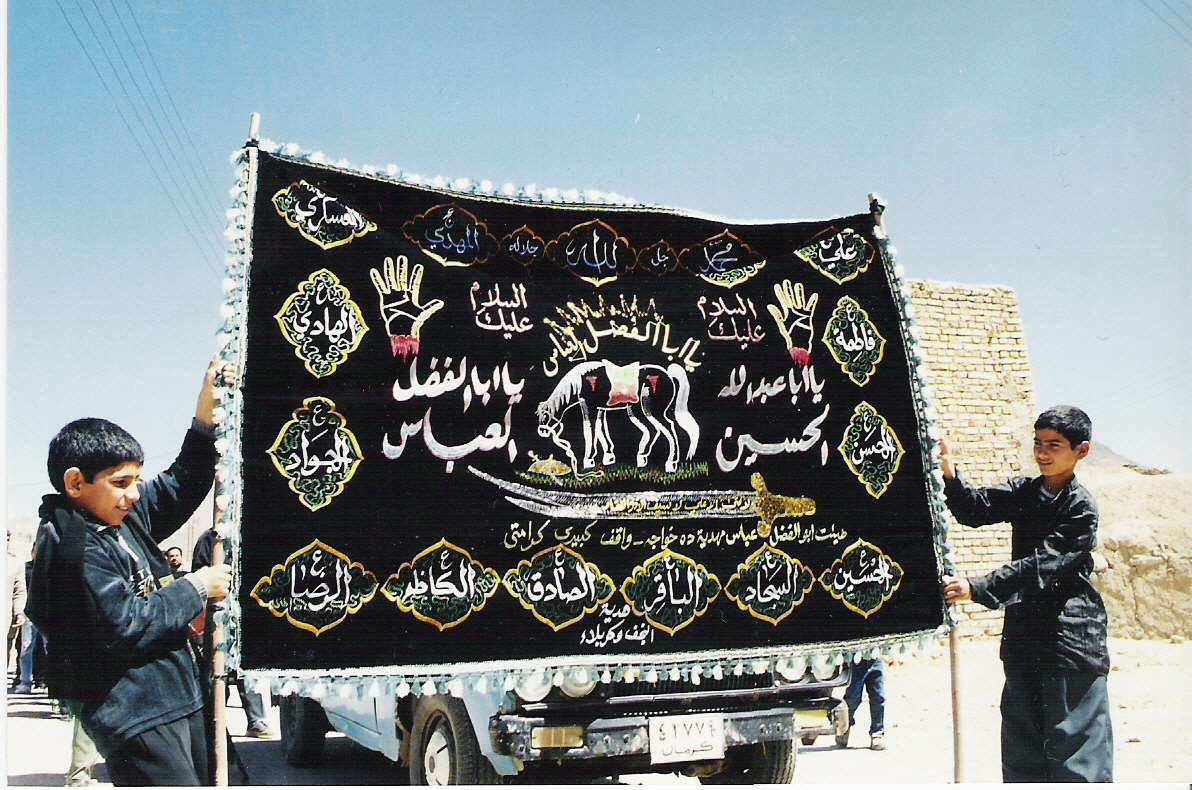
\includegraphics[width=1.97917in,height=1.40972in]{media/image6.jpeg}

\href{https://www.la-croix.com/Religion/Le-Coran-peut-etre-interprete-2021-01-25-1201136852}{Le
Coran peut-il être interprété ?}

Le salafisme, qui représente au moins 40 000 individus, est socialement
dangereux car il impose l'auto-ségrégation, le refus des contacts avec «
ceux qui n'en sont pas ». C'est la raison pour laquelle les spécialistes
des questions de sécurité se refusent à les impliquer dans la lutte
contre le djihadisme. Salafistes et terroristes participeraient à une
même matrice intellectuelle, celle du bien contre le mal, une sorte de
vision sectaire du monde. La différence vient du rapport à la violence :
assumé chez les djihadistes, rejeté chez les salafistes. Leur
fondamentalisme présente l'avantage d'une certaine forme de morale : à
Sartrouville les quartiers salafisés ont vu s'effondrer la toxicomanie
et la délinquance, avec le soutien de la mairie.

\subsection{Confondre l'approche culturelle avec la lutte contre le
terrorisme}

Ces courants ne peuvent être incriminés sur le plan sécuritaire. On
confond donc l'approche culturelle avec la lutte contre le terrorisme. À
moins de changer tout le droit européen, la première doit être menée par
l'éducation, la philosophie, la raison, le débat ; quant à la seconde
elle doit s'appuyer sur le droit et sur des qualifications pénales, et
non sur de vagues impressions de « radicalisation », notion qui n'a
toujours pas été appréhendée de façon rigoureuse en termes sociologiques
et psychologiques.

Comme la guerre d'Algérie nous l'enseigne, une telle manière de
concevoir l'action politique va aboutir à l'effet inverse de celui
recherché : le renforcement de la méfiance collective, le repli
communautaire du côté musulman, l'action violente du côté des « anti »,
et, finalement, la fragmentation sociale et l'insécurité.

\subsection{Islam : les fumées de la radicalisation}

Olivier Hanne, médiéviste (université de Poitiers), chercheur en
islamologie, estime qu'il est très difficile de définir le parcours type
d'une personne radicalisée. Le dernier de trois articles consacrés à
l'islam en France. 
 

Qui parle d'islam aujourd'hui pense aussitôt à la radicalisation. En
2015, on estimait entre 8 000 et 10 000 le nombre de Français
radicalisés. Leurs profils sont si variés qu'il est difficile de donner
des catégories fixes : les mineurs représentent 25 \% des cas, les
femmes 27 \%, les personnes signalées sont plutôt jeunes (entre 16 et 30
ans), leur niveau scolaire est généralement faible, même si l'on
rencontre des diplômés.

La plupart travaillent. Internet représente pour tous ces individus un
passage obligé, même s'il se concrétise différemment : terrain initial
de la radicalisation, facteur de renforcement ou vecteur unique de
l'expression radicale, le partage des contenus djihadistes sur Internet
n'a pas du tout la même fonction chez une adolescente connectée, un
salafiste convaincu et un combattant expérimenté déjà parti en Syrie.

\subsection{Les autorités font feu de tout bois}

De toute évidence, l'attraction pour la radicalité religieuse n'est pas
nécessairement liée à un phénomène de rupture sociale. Les failles de la
société contemporaine (éclatement des familles, déclin des autorités et
des idéologies, chômage, ghettoïsation) créent un terreau facilitateur,
mais nullement déterminant. La frustration individuelle alimente le
recours à des convictions extrêmes, voire le passage à l'acte
terroriste, mais n'est qu'un facteur parmi tant d'autres.

Les autorités font feu de tout bois pour tenter de faire face à une
radicalisation multiforme. En avril 2015, le premier ministre français,
Manuel Valls, annonçait l'ouverture d'une dizaine de centres de
prévention de la radicalisation, dont la plupart furent un échec. Des
sites Internet officiels sont créés et proposent des fiches techniques
contre la radicalisation et le terrorisme, dont le contenu est souvent
simple, voire binaire. Ainsi sur le site
français~\emph{stop-djihadisme.gouv.fr}, un bandeau intitulé «
Radicalisation djihadiste, les premiers signes qui peuvent alerter »
énonce pêle-mêle : « ils se méfient des anciens amis qu'ils considèrent
maintenant comme des impurs » ; « ils changent brutalement leurs
habitudes alimentaires » ; « ils arrêtent d'écouter de la musique car
elle les détourne de leur mission » ; « ils ne regardent plus la
télévision et ne vont plus au cinéma ». Autant de signes extérieurs qui
se rapprochent de l'adolescente anorexique\ldots{} L'efficacité de ces
dispositifs a d'ailleurs été très contestée dès 2015.

\subsection{L'État, tenté d'être omniprésent}

Toute l'entreprise de déradicalisation définit en creux le modèle
positif occidental : monde de loisirs, de consommation, d'épanouissement
personnel et professionnel. Le vocabulaire de la radicalisation masque
le rejet de ce modèle culturel. Et les pouvoirs publics d'hésiter à
appeler leur objectif par son vrai nom : le reconditionnement mental.

Le danger de la déradicalisation se situe dans l'élargissement des
intrusions de l'État : en voulant réinsérer, l'État pénètre dans
l'intimité des individus afin de redéfinir le religieux et lui redonner
une place acceptable. Or, l'État a-t-il compétence pour définir ce
qu'est l'islam, le « bon » islam ? Ne sachant cerner la menace, l'État
est tenté d'être omniprésent, sans en avoir la capacité légale. La
déradicalisation pourrait relever de la posture intellectuelle.

Le problème vient sans doute des hésitations du vocabulaire. Car,
après-tout, qu'est-ce que la radicalisation ? Au
XIX\textsuperscript{e}~le mot anglais~\emph{radical}~était employé pour
désigner les partis politiques britanniques exigeant une réforme
démocratique libérale. Transféré tel quel en France, on l'appliqua aux
partis de gauche, laïques et libéraux qui voulaient réformer la société.

\subsection{Réactions épidermiques}

Le verbe « radicaliser » fut employé régulièrement dans les années
1960-1970 dans une acception politique avec l'idée de « devenir plus
intransigeant, se durcir » ou « plus extrême ». Le premier sens était
donc politique et pas nécessairement négatif. Se déradicaliser était un
synonyme pour « se compromettre ». Appliqué à l'islamisme, le verbe
impose une redéfinition complète des termes : à partir de quand
juge-t-on l'islam intransigeant ou extrême ? par rapport à quelle norme
? à quelle moyenne ?

Les réactions épidermiques qui ont suivi le meurtre de l'enseignant de
Conflans-Sainte-Honorine en octobre 2020 sont tristement révélatrices :
les imams doivent s'exprimer ! les musulmans doivent désavouer le
terrorisme et faire allégeance à la France ! Mais quand ils le font,
c'est encore insuffisant, déloyal et mensonger. Le gouvernement proposa
même qu'ils prient pour la République au cours de la prière collective
du vendredi. Nos références sur la question religieuse restent
tragiquement celles de la Révolution française : comme il y eut les «
prêtres jureurs », adhérant à la loi, contre les « prêtres réfractaires
», obstinés dans leur obéissance à Rome, de la même façon il nous faut
des « imams jureurs », intimement républicains. L'État se retrouve donc
juge des reins et des cœurs.

\bibliography{Theo}
%\bibliographystyle{siam}
%\printbibliography

\listoftheorems[ignoreall,show={Def}]
%Les courants contemporains de l’islam Glossaire général

\mn{Vérifier les termes}

bid‘a : innovation ; pratique « déviante ».

da‘wa : invitation ; prédication – appel à la conversion (dans les deux sens).

fasiq : pécheur ; mauvais musulman.

fiqh : compréhension ; corpus du droit musulman.

fitna: discorde, querelle ; conflit interne au monde musulman.

hadith : récit d’un dire ou faire du Prophète, rapporté par ses compagnons.

hajj : pèlerinage annuel à La Mecque.

hijra (héjire) : « exode » - départ de Mahomet pour Médine (622).

‘ibadat : culte ; partie du droit traitant du culte.

ijma‘ : consensus ; consensus des ulama sur un point de droit.

ijtihad : effort ; effort d’interprétation du Coran.

imam : chef suprême de la communauté musulmane ; successeur du Prophète, utilisé communément par les chiites pour Ali et ses descendants.

islah : réforme.

isnad : chaîne ; chaîne de transmission des hadiths.

jihad : lutte ; soit intérieure, contre ses propres faiblesses ; soit extérieure, contre les ennemis de la communauté musulmane.

ka‘aba : monument cubique noir situé au centre de la grande mosquée de La Mecque ; selon les musulmans, désigne l’emplacement du premier autel élevé par Abraham pour le Dieu unique. Point vers lequel se dirigent les musulmans pour prier.

kafir : infidèle, mécréant

khalifa (calife) : successeur, représentant ; successeur du Prophète et chef de la communauté musulmane (sunnisme).

madrasa : école ; lieu où est assuré la transmission du savoir religieux.

mihrab : niche indiquant la direction de La Mecque dans une mosquée.
 
mu‘amalat : relations ; partie du droit traitant des relations humaines.

qibla : orientation de la prière rituelle (salat), correspondant à la direction de La Mecque.

qiyas : raisonnement par analogie (domaine du droit)

salat : prière rituelle.

seyyed : prince, chef ; descendant du Prophète par Hossein ou Hassan, fils d’Ali.

shari‘a : sentier, voie ; loi divine.

sheykh (cheykh) : vieil homme ; chef d’une tribu ; chef religieux ; personne à la tête d’une congrégation soufie, ayant la capacité de guider ses disciples.

shirk : associationnisme : fait d’adorer d’autres êtres en dehors de Dieu.

shura : principe de consultation soufi : mystique musulman sourate : chapitre du Coran
sunna : coutume ; pratiques du Prophète et de la première communauté musulmane, faisant autorité pour guider le mode de vie des croyants et déterminer la loi religieuse.

tafsir : commentaire du Coran.

tajdid : renouveau (=>mujaddidi : qui renouvelle)

taqlid : imitation ; imitation stérile des anciens (par opposition à l’ijtihad).

tariqa : voie : confrérie soufie.

tawhid : unicité (divine). Dogme fondamental de l’islam.

ulama (oulémas) : terme collectif pour désigner les lettrés musulmans.

umma : peuple ou communauté ; communauté islamique dans son ensemble.

waqf : bien immobilier ou foncier dit « de-main-morte », dépendant des institutions religieuses.

zakat : aumône rituelle, obligatoire pour les croyants.

%\listoftheorems


\end{document}